\documentclass[german,10pt]{article}      
\usepackage{makeidx}
\usepackage{babel}            % Sprachunterstuetzung
\usepackage{amsmath}          % AMS "Grundpaket"
\usepackage{amssymb,amsfonts,amsthm,amscd} 
\usepackage{mathrsfs}
\usepackage{rotating}
\usepackage{sidecap}
\usepackage{graphicx}
\usepackage{color}
\usepackage{fancybox}
\usepackage{tikz}
\usetikzlibrary{arrows,snakes,backgrounds}
\usepackage{hyperref}
\hypersetup{colorlinks=true,
                    linkcolor=blue,
                    filecolor=magenta,
                    urlcolor=cyan,
                    pdftitle={Overleaf Example},
                    pdfpagemode=FullScreen,}
%\newcommand{\hyperref}[1]{\ref{#1}}
%
\definecolor{Gray}{gray}{0.80}
\DeclareMathSymbol{,}{\mathord}{letters}{"3B}
%
\newcounter{num}
\renewcommand{\thenum}{\arabic{num}}
\newenvironment{anmerkungen}
   {\begin{list}{(\thenum)}{%
   \usecounter{num}%
   \leftmargin0pt
   \itemindent5pt
   \topsep0pt
   \labelwidth0pt}%
   }{\end{list}}
%
\renewcommand{\arraystretch}{1.15}                % in Formeln und Tabellen   
\renewcommand{\baselinestretch}{1.15}                 % 1.15 facher
                                                      % Zeilenabst.
\newcommand{\Anmerkung}[1]{{\begin{footnotesize}#1 \end{footnotesize}}\\[0.2cm]}
\newcommand{\comment}[1]{}
\setlength{\parindent}{0em}           % Nicht einruecken am Anfang der Zeile 

\setlength{\textwidth}{15.4cm}
\setlength{\textheight}{23.0cm}
\setlength{\oddsidemargin}{1.0mm} 
\setlength{\evensidemargin}{-6.5mm}
\setlength{\topmargin}{-10mm} 
\setlength{\headheight}{0mm}
\newcommand{\identity}{{\bf 1}}
%
\newcommand{\vs}{\vspace{0.3cm}}
\newcommand{\noi}{\noindent}
\newcommand{\leer}{}

\newcommand{\engl}[1]{[\textit{#1}]}
\parindent 1.2cm
\sloppy

         \begin{document} 

\begin{center}
{\large\bf Inhalt}\\
\today
\end{center}
\thispagestyle{empty}

\noindent
{\bf Physik des Klimas}\\[0.4cm]
\hyperref[chap_Klima1]{Solarkonstante und Paleoklima}\\[0.2cm]
\hyperref[chap_Klima3]{Klimamodelle}\\[0.4cm]
{\bf Quantentheorie}\\[0.4cm]
\hyperref[chap_QuBit]{Das QuBit}\\[0.2cm]
\hyperref[chap_Interferometer]{Interferometer}\\[0.2cm]
\hyperref[chap_BB84]{BB84 - Quantenkryptographie}\\[0.2cm]
\hyperref[chap_Quantenradierer]{Quantenradierer}\\[0.4cm]
{\bf Klassische Systeme}\\[0.4cm]
\hyperref[chap_SI]{SI-Einheiten}\\[0.2cm]                          %  01
\hyperref[chap_Kalender]{Kalendersysteme}\\[0.2cm]       % 02
\hyperref[chap_Zeitgleichung]{Die Zeitgleichung}\\[0.2cm] % 03
\hyperref[chap_Zeitsysteme]{Zeitsysteme}\\[0.2cm]          % 04
\hyperref[chap_Uhren]{Zeitmessung}\\[0.2cm]                   % 05
\hyperref[chap_Gezeiten1]{Die Gezeiten - Ebbe und Flut}\\[0.2cm] % 06
\hyperref[chap_Gezeiten2]{Gezeiten und Tagesl\"ange}\\[0.2cm] % 07
\hyperref[chap_Nachthimmel]{Der Nachthimmel}\\[0.2cm]  % 08
\hyperref[chap_Kosm_Entfernung]{Die Kosmische Entfernungsleiter}\\[0.2cm] % 09
\hyperref[chap_Landkarte]{Landkarten und der metrische Tensor}\\[0.4cm] % 10
{\bf Spezielle Relativit\"atstheorie - SRT}\\[0.4cm]
\hyperref[chap_Grundlagen]{Grundlagen der SRT}\\[0.2cm]      %  01
\hyperref[chap_Philosophie-SRT]{Philosophischer Hintergrund der SRT}\\[0.2cm]   % 03
\hyperref[chap_SRT-Effekte]{SRT - Effekte}\\[0.2cm]               % 04
\hyperref[chap_Zwilling]{Das Zwillingsparadoxon}\\[0.2cm]      % 05
\hyperref[chap_Rindler]{Beschleunigte Systeme und das Rindler-Universum}\\[0.2cm]  % 06

\documentclass[german,10pt]{book}      
\usepackage{makeidx}
\usepackage{babel}            % Sprachunterstuetzung
\usepackage{amsmath}          % AMS "Grundpaket"
\usepackage{amssymb,amsfonts,amsthm,amscd} 
\usepackage{mathrsfs}
\usepackage{rotating}
\usepackage{sidecap}
\usepackage{graphicx}
\usepackage{color}
\usepackage{fancybox}
\usepackage{tikz}
\usetikzlibrary{arrows,snakes,backgrounds}
\usepackage{hyperref}
\hypersetup{colorlinks=true,
                    linkcolor=blue,
                    filecolor=magenta,
                    urlcolor=cyan,
                    pdftitle={Overleaf Example},
                    pdfpagemode=FullScreen,}
%\newcommand{\hyperref}[1]{\ref{#1}}
%
\definecolor{Gray}{gray}{0.80}
\DeclareMathSymbol{,}{\mathord}{letters}{"3B}
%
\newcounter{num}
\renewcommand{\thenum}{\arabic{num}}
\newenvironment{anmerkungen}
   {\begin{list}{(\thenum)}{%
   \usecounter{num}%
   \leftmargin0pt
   \itemindent5pt
   \topsep0pt
   \labelwidth0pt}%
   }{\end{list}}
%
\renewcommand{\arraystretch}{1.15}                % in Formeln und Tabellen   
\renewcommand{\baselinestretch}{1.15}                 % 1.15 facher
                                                      % Zeilenabst.
\newcommand{\Anmerkung}[1]{{\begin{footnotesize}#1 \end{footnotesize}}\\[0.2cm]}
\newcommand{\comment}[1]{}
\setlength{\parindent}{0em}           % Nicht einruecken am Anfang der Zeile 

\setlength{\textwidth}{15.4cm}
\setlength{\textheight}{23.0cm}
\setlength{\oddsidemargin}{1.0mm} 
\setlength{\evensidemargin}{-6.5mm}
\setlength{\topmargin}{-10mm} 
\setlength{\headheight}{0mm}
\newcommand{\identity}{{\bf 1}}
%
\newcommand{\vs}{\vspace{0.3cm}}
\newcommand{\noi}{\noindent}
\newcommand{\leer}{}

\newcommand{\engl}[1]{[\textit{#1}]}
\parindent 1.2cm
\sloppy

         \begin{document}  \setcounter{chapter}{0}


\chapter{Physik des Klimas I\\Solarkonstante und Paleoklima}
\label{chap_Klima1}
% Kap x

\info{Thomas Filk; 30.03.2024}%
Unser Klima wird in erster Linie durch die Sonne bestimmt. Von ihr stammt die Energie,
die nahezu s\"amtliche dynamischen Vorg\"ange auf der Erde antreibt. 
Eine zweite Energiequelle besteht in Zerfallsprozessen radioaktiver Elemente im Erdinneren.
Diese Energieform k\"onnen wir jedoch f\"ur das Verst\"andnis des Klimas vernachl\"assigen.

Die Energieform, die in der Sonne durch Kernfusionsprozesse entsteht - streng genommen sollte
man nat\"urlich immer von \glqq Umwandlung\grqq\ sprechen, d.h., bei Kernfusionspozessen wird
Kernenergie in thermische (Bewegungs-)Energie, Strahlungsenergie sowie in Neutrinos umgewandelt -, 
erreicht uns in Form 
von elektromagnetischer Strahlung, haupts\"achlich im sichtbaren Bereich. Die Oberfl\"ache der
Sonne hat eine Temperatur von rund 5800\,Kelvin und die zugeh\"orige thermische Strahlung
hat ihr Maximum bei rund 500\,nm, das entspricht Licht im gr\"un-blauen Bereich. 

Der erste Abschnitt wird auf die Solarkonstante eingehen, d.h., die Menge an Energie, die pro
Zeiteinheit (Sekunde) und pro Fl\"acheneinheit (Quadratmeter) bei der Erde oberhalb der
Atmosph\"are ankommt. In diesem Zusammenhang gehen wir auch auf Ph\"anomene wie die Albedo
der Erde ein. Au\ss erdem betrachten wir verschiedene Faktoren, die in der Vergangenheit
einen Einfluss auf die Solarkonstante bzw.\ die Einstrahlung der Sonnenstrahlung auf die
Erde gehabt haben und damit unser Klima beeinflusst haben k\"onnten.
Schlie\ss lich betrachten wir auch kurz das Gebiet der Pal\"aoklimatologie, das sich mit
dem Klima im Verlauf der Erdgeschichte besch\"aftigt. 


\section{Die Solarkonstante}

Die Solarkonstante ist definiert als das langj\"ahrige Mittel der Intensit\"at pro Fl\"acheneinheit der 
Sonneneinstrahlung oberhalb der Erdatmosph\"are.\index{Solarkonstante} 
Die Intensit\"at ist dabei die Energie, die pro Sekunde 
auf eine bestimme Fl\"ache - in diesem Fall ein Quadratmeter senkrecht zur Strahlungsrichtung - trifft
(siehe Abb.\ \ref{fig_solar_constant}). 
Die IAU (International Astronomical Union) hat 2015 die Solarkonstante aufgrund neuerer
Messungen auf den Wert
\begin{equation}
               S = 1361\,{\rm J \cdot s^{-1} \cdot m^{-2}}
\end{equation}
festgelegt. In \"alteren B\"uchern findet man oft den Wert $S= 1367\,{\rm J \cdot s^{-1} \cdot m^{-2}}$, der
von 1982 bis 2015 G\"ultigkeit hatte. Heute misst man die Solarkonstante mit Satelliten, wobei die
gemessenen Intensit\"aten auf den mittleren Abstand Erde-Sonne - die Astronomische Einheit - 
umgerechnet wird.

\begin{SCfigure}[30][htb]
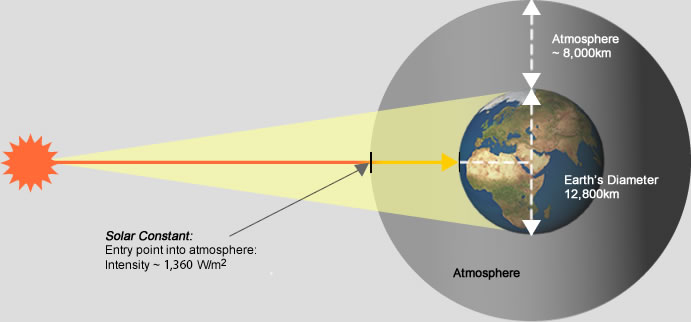
\includegraphics[scale=0.4]{./Bilder/solar-constant.jpg}
\caption{\label{fig_solar_constant}%
Definition der Solarkonstanten. Die gemessene Intensit\"at der Sonnenstrahlung
oberhalb der Erdatmosph\"are wird auf den mittleren Abstand Sonne-Erde umgerechnet.
(aus \cite{Solar})}
\end{SCfigure}


\subsection{Sonnenaktivit\"at}

Streng genommen handelt es sich bei der Solarkonstanten nicht um eine Naturkonstante. Sie unterliegt
kleinen Schwankungen.\index{11-Jahres-Zyklus der Sonne}\index{Sonnenzyklus} 
Eine winzige Schwankung entsteht durch den 11-Jahres-Zyklus der 
Sonnenaktivit\"at. Im sichtbaren Bereich machen diese Schwankungen aber nur rund 0,1\% aus. Lediglich
im UV- bzw.\ im R\"ontgen-Bereich k\"onnen diese Schwankungen wesentlich gr\"o\ss er sein, allerdings
wird diese Strahlung in h\"oheren Schichten unserer Atmosph\"are reflektiert bzw.\ absorbiert und 
erreicht den Erdboden gr\"o\ss tenteils nicht. Allerdings lassen sich Schwankungen in
der mittleren Jahrestemperatur von der Gr\"o\ss enordnung von $0,1^\circ$C mit einer Periode von 11
Jahren \"uber l\"angere Zeitr\"aume nachweisen. 
Au\ss erdem gab es in der Vergangenheit h\"aufiger Perioden, in denen die Sonne
insgesamt weniger aktiv war und die m\"oglicherweise zu kleinen Eiszeiten gef\"uhrt haben. Bekannt sind solche
Perioden in der Zeit zwischen dem 14.\ und 18.\ Jahrhundert (das sogenannte Sp\"orer-Minimum und das
Maunder-Minimum; wobei ein direkter Bezug zum Klima in dieser Periode immer noch umstritten ist), 
beispielsweise durch Wintergem\"alde von 
Pieter Bruegel dem \"Alteren und seinen S\"ohnen. 

Seit Beginn des 17.\ Jahrhunderts (seit der Erfindung des
Teleskops) wurden die Sonnenflecken direkt beobachtet, sodass es gute Aufzeichnungen
gibt. F\"ur die Perioden\index{Proxy!Sonnenaktivit\"at}\index{14-C@${}^{14}C}\index{10-Be@${}^{10}Be} 
davor eignen sich manche Isotopmessungen (z.B.\ ${}^{14}$C und ${}^{10}$Be).
Diese Isotope entstehen haupts\"achlich in der Atmosph\"are durch den Einfluss der kosmischen Strahlung, 
die wiederum durch eine starke Sonnenaktivit\"at und die damit verbundenen Sonnenwinde 
abgeschw\"acht wird. Dies f\"uhrt zu einer Korrelation zwischen der H\"aufigkeit dieser Isotope in
Bohrproben, die auf bestimmte Zeiten datiert werden k\"onnen, und der Sonnenaktivit\"at: H\"ohere
Isotopenanteile lassen auf geringere Sonnenaktivit\"at schlie\ss en, da zu diesen Zeiten die kosmische
Strahlung ungehinderter in die Atmosph\"are dringen konnte.

\subsection{Milankovi\'c-Zyklen}

F\"ur unser Klima\index{Milakonvi\`c, Milan}\index{Milankovi\`c-Zyklen}
relevante Schwankungen sind (vermutlich) die sogenannten Milankovi\'c-Zyklen, benannt nach
dem serbische Mathematiker Milutin Milankovi\'c (1879-1958). Hierbei handelt es sich um regelm\"a\ss ige
Oszillationen in den Parametern der Erdumlaufbahn um die Sonne. Diese Parameter sind
insbesondere die Exzentrizit\"at der Erdbahn, die Neigung der Erdachse und die
Pr\"azession der Erdachse.

\subsubsection{Die Exzentrizit\"at der Erdumlaufbahn} 

In einem reinen Zwei-K\"orper-Problem mit einer $1/r^2$-Kraft\index{Exzentrizit\"at}\index{Kepler-Problem, 2-K\"orper-}
(manchmal als nicht-relativistisches Kepler-Problem bezeichnet) bewegt sich ein leichter K\"orper (Erde)
um einen schweren K\"orper (Sonne) auf einer elliptischen Bahn, wobei sich der schwere K\"orper
in einem der Brennpunkte der Ellipse befindet. Dies gilt ganz allgemein f\"ur die Relativkoordinate
zwischen den beiden Himmelsk\"orpern, auch wenn die Masse des leichteren Himmelsk\"orpers
im Vergleich zu dem schwereren Himmelsk\"orper nicht vernachl\"assigt werden kann. In diesem Fall
bewegen sich die beiden K\"orper um einen gemeinsamen Schwerpunkt, der sich in einem der
Brennpunkte der Ellipse befindet.  

Durch den Einfluss der anderen Planeten, insbesondere Jupiter und Saturn, ver\"andert sich die 
Bahnkurve der Erde jedoch im Verlauf der Zeit. Insbesondere kann auch die Exzentrizit\"at der
elliptischen Bahn zwischen einer fast kreisf\"ormigen Erdumlaufbahn ($\epsilon = 0,0006$) und einer
schwach elliptischen Bahn ($\epsilon =0,058 $) variieren \cite{Wikipedia_Milankovic}. 
Diese Werte schwanken periodisch mit einer Periode von rund
405\,000 Jahren, wobei auch Unterzyklen von der Gr\"o\ss enordnung von 100\,000 Jahren existieren. 

Derzeit betr\"agt der Wert rund $\epsilon= 0,0167$, was einer Schwankung in der Entfernung zwischen
Erde und Sonne im Bereich zwischen\index{Exzentrizi\"atsschwankungen}
147,09 Millionen Kilometern und 152,10 Millionen Kilometern entspricht. Obwohl die Differenz in diesen
Werten nur rund 3.4\% ausmacht, bedeutet dies f\"ur die Intensit\"at der Sonnenstrahlung
eine Schwankung von rund 6,8\% im Verlauf eines Jahres \hyperref[Anm-1]{(1)}. 
Bei einer entsprechend gr\"o\ss eren Exzentrizit\"at sind auch diese 
Schwankungen gr\"o\ss er und k\"onnen bis zu 24\% ausmachen.

\subsubsection{Neigung der Erdachse} 

Im Vergleich zur Ekliptik, also der Ebene der Erdumlaufbahn\index{Erdachse!Neigung}
um die Sonne, ist die Drehachse der Erde um rund $23,5^\circ$ geneigt. Dieser Neigungswinkel
\"andert sich aufgrund der Einfl\"usse anderer Planeten mit einer Periode von rund 41.000 Jahren
und schwankt zwischen $22,1^\circ$ und $24,5^\circ$.

Auch diese Schwankung hat zun\"achst einen jahreszeitlichen Einfluss auf unser Klima: Ist der
Neigungswinkel gr\"o\ss er, ist der Unterschied im Einfallswinkel der Sonne zwischen Sommer und
Winter entsprechend gr\"o\ss er, d.h., die jahreszeitlichen Schwankungen fallen st\"arker aus. 
Das wiederum kann einen Einfluss darauf haben, wie stark Schnee- und Eisfl\"achen im Sommer
abtauen und sich somit zur\"uckbilden. Au\ss erdem haben diese Schwankungen einen Einfluss
auf verdunstende Wassermengen in h\"oheren Breitengraden und somit auf den dortigen Niederschlag, 
was sich beispielsweise im Winter auf erh\"ohten Schneezuwachs bei Gletschern auswirken kann. 

\subsubsection{Pr\"azession der Erdachse} 

Da die Erde keine ideale Kugelform hat sondern entlang der Erdachse\index{Praezession@Pr\"azession}
etwas abgeplattet ist, also entlang des \"Aquators etwas \glqq dicker\grqq\ als entlang von L\"angengraden
(der Abstand vom Erdzentrum zum Nord- bzw.\ S\"udpol ist um rund 21 Kilometer kleiner als der 
Abstand vom Erdzentrum zum \"Aquator, wobei hier f\"ur die Erde vereinfachend die\index{Erdform, Rotationsellipsoid} 
Form eines
Rotationsellipsoids angenommen wird). Der gravitative Einfluss von Sonne und Mond (in geringerem Ma\ss\
auch der von anderen Planeten, insbesondere Jupiter und Saturn) bewirkt ein Drehmoment, das 
die Erdachse aufrichten w\"urde, falls sich die Erde nicht drehte. Wegen der Drehimpulserhaltung wird
die Drehachse zur Seite gedreht und rotiert langsam um eine Senkrechte zur Erdbahn ((Bild!)).
Diese Drehung bezeichnet man als Pr\"azession. Sie hat eine Periode von rund 25\,800 Jahren.

Der Haupteffekt der Neigung der Erdachse sind die Jahreszeiten, die auf der Nord- und S\"udhalbkugel
der Erde um ein halbes Jahr relativ zueinander verschoben sind. Die Pr\"azession bewirkt, zusammen mit
den anderen Orbitalparametern, dass die Unterschiede zwischen den Jahreszeiten (insbesondere
zwischen Sommer und Winter) hinsichtlich ihrer Intensit\"at verschieden stark ausfallen k\"onnen.
Wenn beispielsweise die Elliptizit\"at der Erbahn (d.h.\ die Exzentrizit\"at) sehr gro\ss\ ist, kann
die Richtung der Erdachse relativ zu den Hauptachsen die Strahlungsunterschiede zwischen Sommer
und Winter entweder verst\"arken (wenn der Sommer mit dem Perihel zusammenf\"allt) oder
abschw\"achen (wenn Sommer mit dem Aphel zusammenf\"allt). 

Ein weiterer wesentlicher Faktor f\"ur das Klima ist, dass die Nordhalbkugel der Erde gr\"o\ss ere
Landmassen hat als die S\"udhalbkugel, die eine gr\"o\ss ere Wasserfl\"ache hat. Insofern spielt es
eine Rolle, ob die oben erw\"ahnte Verst\"arkung der Unterschiede zwischen Sommer und Winter
f\"ur die Nord- oder f\"ur die S\"udhalbkugel zutrifft.  

W\"ahrend man in der physikalischen und astrophysikalischen Literatur f\"ur die Pr\"azession der
Erde einen Wert von 25\,800 (oder aufgerundet 26\,000) Jahren findet, findet man in der
Literatur zur Klimaphysik bzw.\ zu den Milankovi\'c-Zyklen
oftmals einen Wert von 23\,000 Jahren. F\"ur die Physik (z.B.\ die
Bestimmung des Fr\"uhlingspunkts und den damit zusammenh\"angenden Jahreszeiten) ist
die Richtung der Erdachse relativ zur Sonne wichtig. F\"ur die Klimaforschung ist man eher an der
Richtung der Erdachse relativ zum Perihel bzw.\ Aphel interessiert. 
Wegen der Periheldrehung\index{Periheldrehung}
der Erde, verschieben sich diese Punkte aber langsam. Der kombinierte Effekt von 
Pr\"azession und Periheldrehung f\"uhrt zu der verk\"urzten Periode von 23\,000 Jahren. 


\subsection{Das Sonnenalter}

Auf sehr langen Zeitskalen nimmt die Solarkonstante zu: in 100 Millionen Jahren um rund 1\% 
\cite{Wikipedia_Solarkonstante}. Zu Beginn der Erdgeschichte betrug die 
Sonnenintensit\"at nur\index{Sonnenintensit\"at!in fr\"uheren Zeiten}\index{Fain young Sun paradox}
rund 70\% ihres heutigen Werts. Das Klima auf der Erde h\"atte somit wesentlich k\"alter sein m\"ussen
und alles Wasser auf der Erde h\"atte gefroren sein m\"ussen. Es gibt aber deutliche Hinweise
darauf, dass es insgesamt meist w\"armer auf der Erde gewesen ist. Dies bezeichnet man als
das  \textit{Faint young Sun paradox} \cite{Wikipedia_Faint}. Eine m\"ogliche L\"osung ist, dass der
Kohlendioxidgehalt der Atmosph\"are in fr\"uheren Zeiten (z.B.\ aufgrund von Vulkanismus)
wesentlich h\"oher war als heute. Diese Frage ist aber noch nicht endg\"ultig gekl\"art.

\section{Die Albedo}

Die Albedo\index{Albedo} 
ist ein Ma\ss\ daf\"ur, wie stark ein Gegenstand eine Strahlung reflektiert. Es ist so etwas
wie der totale elastische Wirkungsquerschnitt eines Gegenstands f\"ur elektromagnetische Strahlung. 
Allerdings handelt es sich nicht um eine Fl\"ache, sondern um ein Verh\"altnis: das Verh\"altnis
von reflektierter Intensit\"at zu eingestrahlter Intensit\"at. Man kann die Albedo als Funktion
der Wellenl\"ange bzw.\ der Frequenz betrachten (da es um die reflektierte Strahlung geht, soll die
Wellenl\"ange bzw.\ Frequenz erhalten bleiben), meist interessiert man sich aber f\"ur die
Summe \"uber das gesamte Spektrum. 

Wenn man ein Foto von der Erde betrachtet, aufgenommen von einem Satelliten oder, besser noch, 
von einer Raumsonde oder Rakete auf dem Weg zum Mond oder einem anderen Ort im Sonnensystem,   
ist alles, was man von der Erde sieht, reflektierte Strahlung (siehe Abb.\ \ref{fig_NASA_Welt}). 
Auf einem solchen Bild sieht man
sofort, welche Teile der Erde eine hohe und welche eine niedrige Albedo haben: Schnee- und Wolkenfelder
haben eine hohe Albedo, ebenso Eisfelder; Wasser und W\"alder haben eine sehr niedrige Albedo. 
Sand bzw.\ W\"uste oder Steppen haben eine mittlere Albedo. 

\begin{SCfigure}[30][htb]
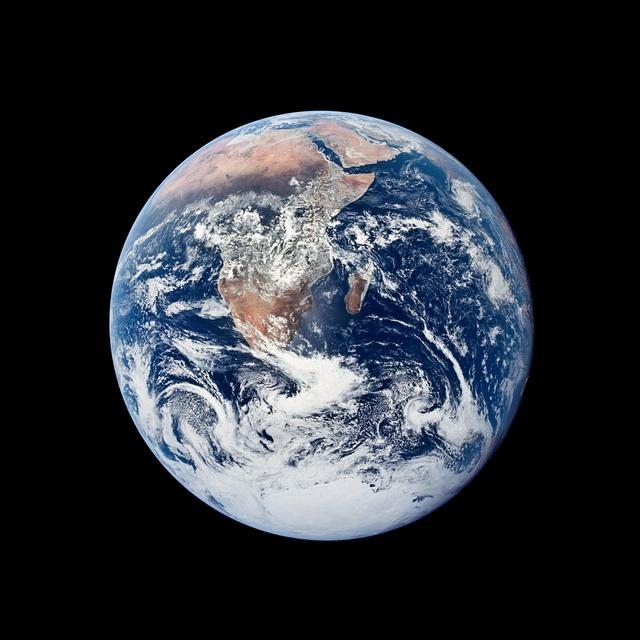
\includegraphics[trim=70 70 70 70, clip, width = 0.33\textwidth]{./Bilder/as17-Albedo-orig.jpg}
\caption{\label{fig_NASA_Welt}%
Die Erde, aufgenommen von der Crew der Apollo-17 Mission im Jahre 1972. Deutlich erkennbar sind
die Antarktis, der afrikanische Kontinent, die Insel Madagaskar und die saudi-arabische Halbinsel. Die sehr
stark reflektierenden Gebiete sind wei\ss, das sind Schnee- und Wolkenfl\"achen. Die W\"usten sind
deutlich heller als Waldgebiete oder Grasfl\"achen. 
Sehr dunkel sind die Meere. Diese Helligkeiten entsprechen der
Albedo der jeweiligen Fl\"achen. (aus \cite{NASA_World})}
\end{SCfigure}

Die Albedo hat einen sehr gro\ss en Einfluss auf unser Klima. Je gr\"o\ss er die Albedo eines
Planeten ist, umso geringer ist (bei gleichbleibenden anderen Faktoren) die Oberfl\"achenerw\"armung. 
W\"ahrend die Erde insgesamt eine Albedo von 0,3 hat, hat beispielsweise der Planet Venus\index{Albedo!Venus} 
aufgrund seiner dichten Wolkenschicht eine Albedo von 0,7. Obwohl Venus deutlich n\"aher an der Sonne
ist als die Erde und aus diesem Grunde eine doppelt so hohe Solarkonstante hat, w\"are ihre
Temperatur aufgrund der Albedo k\"uhler als die der Erde. Tats\"achlich ist ihre Oberfl\"achentemperatur 
jedoch wesentlich h\"oher (bei $460^\circ$C). Der Grund ist der Treibhauseffekt: Die Atmosph\"are
von Venus besteht zu 96\% aus Kohlendioxid.\index{Venus!Albedo}\index{Venus!Atmosph\"are}\index{Atmosph\"are!Venus} 

\section{Aufbau der Atmosph\"are}

Die Atmosph\"are der Erde\index{Erdatmosph\"are}\index{Atmosph\"are!Erde} 
wird in verschiedene Schichten unterteilt, von denen die untersten
drei Schichten - die Troposph\"are, die Stratosph\"are und die Mesosph\"are - den gr\"o\ss ten
Einfluss auf unser Klima haben. Sie sind durch ihre Temperaturgradienten definiert. Die beiden
dar\"uber liegenden Schichten - die Thermosph\"are (100--600\,km) und die Exosph\"are
(600--200\,000\,km) - haben keinen direkten Einfluss auf unser Wetter bzw.\ Klima. 

\subsection{Die Troposph\"are}

Die Troposph\"are\index{Troposph\"are} 
ist die unterste Atmosph\"arenschicht, in der sich nahezu alle Wettervorg\"ange
abspielen. Definiert ist sie durch einen negativen Temperaturgradienten, d.h., in dieser Schicht
nimmt die Temperatur mit der H\"ohe ab. Sie erstreckt sich an den Polen bis in eine H\"ohe von
rund 6--8\,km, in den Tropen bis zu einer H\"ohe von 12--18\,km. Im Durchschnitt hat sie eine
H\"ohe von 13\,km. 

Die Abnahme der Temperatur h\"angt mit der Druckabnahme zusammen. Der Druck nimmt
nahezu exponentiell mit der H\"ohe ab (dies gilt auch weit \"uber die Troposph\"are hinaus). Aus diesem
Grund dehnt sich aufsteigende Luft aus
(sie passt sich praktisch instantan dem Umgebungsdruck an) und wird dabei k\"uhler. Dieser
Vorgang erfolgt nahezu adiabatisch, d.h., es findet kein W\"armeaustausch mit der Umgebung
statt. Aus diesem Grund nimmt die Temperatur mit der H\"ohe ab. 

Eine instabile Wetterlage liegt
vor, wenn die Abk\"uhlung eines Luftpakets bei seinem Aufstieg aufgrund des verminderten
Drucks langsamer erfolgt, als es der Temperatur der Umgebung entspricht. In diesem Fall hat
das Luftpaket in einer bestimmten H\"ohe eine h\"ohere Temperatur als die Umgebung, aber
es hat denselben Druck. H\"ohere Temperatur aber gleicher Druck bedeutet, dass die Dichte
des Luftpakets geringer ist als die Dichte der Umgebungsluft und somit ist das Luftpaket leicher
und steigt weiter in die H\"ohe. Es findet somit eine Konvektion statt. Nimmt die Temperatur eines
Luftpakets jedoch beim Aufstieg schneller ab, als die Temperatur der Umgebung, bleibt das
Luftpaket dichter und steigt nicht weiter bzw.\ sinkt wieder. In diesem Fall ist die Lage stabil.
Insbesondere herrscht eine stabile Wetterlage bei einer Inversionslage, 
d.h., wenn die\index{Inversionslage}
Temperatur lokal mit der H\"ohe zunimmt. In aufsteigender Luft nimmt der Druck immer noch
ab, sie k\"uhlt sich somit ab und ihre Temperatur bleibt unter der Temperatur der Umgebung.
Somit ist dieses Luftpaket dichter als die Luft der Umgebung und sinkt wieder ab.   

Gehen wir an der Erdoberfl\"ache von einer mittleren Temperatur von rund $18^\circ$C aus,
so kann die Temperatur bis zur Obergrenze der Troposph\"are auf rund $-50^\circ$C bis $-60^\circ$C
abnehmen.

\subsection{Die Stratosph\"are}

Oberhalb der Troposph\"are\index{Stratosph\"are} 
beginnt die Stratosph\"are, wobei diese beiden Atmosph\"arenschichten
durch die sogenannte Tropopause\index{Tropopause} 
getrennt sind. In der Stratosph\"are nimmt die Temperatur
mit zunehmender H\"ohe zu und kann in rund 50\,km H\"ohe wieder nahezu bei $0^\circ$C
liegen. In der Stratosph\"are liegt die Ozonschicht.\index{Ozonschicht} 
Das Ozon absorbiert die UV-Strahlung,
was zu einer Erw\"armung f\"uhrt. Da hier die h\"oher liegenden Luftschichten eine h\"ohere
Temperatur haben, kommt es in der Stratosph\"are praktisch nicht mehr zur Konvektion. 
Wolken, z.B.\ Gewitterwolken, die bis in die Stratosph\"are reichen, bilden dort meist einen
sogenannten Amboss, d.h.\ eine flache ausgedehnte Struktur, in der keine Konvektion mehr
stattfindet. 

\subsection{Die Mesosph\"are}

Oberhalb der Stratosph\"are in rund 50--60\,km H\"ohe beginnt die Mesosph\"are. 
Sie reicht bis\index{Mesosph\"are} 
ungef\"ahr 80--90\,km. In dieser Schicht findet man kaum noch Ozon, sodass die Temperatur 
in der Mesosph\"are wieder abnimmt, teilweise bis deutlich unter $-140^\circ$C. Dies ist 
die k\"alteste Schicht unserer Atmosph\"are.

\subsection{Thermosph\"are und Exosph\"are}

In rund 85\,km H\"ohe beginnt die Thermosph\"are.\index{Thermosph\"are}\index{Exosph\"are} 
Hier ist die Luft so d\"unn, dass
die Atome von einzelnen Photonen auf sehr hohe Geschwindigkeiten beschleunigt
werden k\"onnen, und da die mittlere Wegl\"ange der Atome bzw.\ Molek\"ule sehr
gro\ss\ ist, kommt es kaum zu einem Austausch. Die Temperatur nimmt daher wieder
zu, bis teilweise auf \"uber $1000^\circ$C. 

Oberhalb der Thermosph\"are in rund 600--700\,km H\"ohe beginnt die sogenannte
Exosph\"are. Die Temperatur \"andert sich hier nicht - die Luft wird so d\"unn, dass man
von Temperatur im thermodynamischen Sinne kaum sprechen kann. Der \"Ubergang
zwischen beiden Schichten ist flie\ss end. Eine Definition definiert die Grenze zwischen
diesen beiden Schichten \"uber die mittlere freie Wegl\"ange der Atome bzw.\ Teilchen.
Als Obergrenze der Exosph\"are wird meist die Schicht definiert, in der die Sonnenwinde
einen gr\"o\ss eren Einfluss auf die Teilchen haben als das Gravitationsfeld der Erde.
Diese Schicht liegt bei rund 200\,000\,km. 

\subsection{Homosph\"are und Heterosph\"are}

Bis zu ungef\"ahr der gleichen H\"ohe wie die Mesosp\"are, d.h.\ bis rund 85\,km, 
reicht auch die sogenannte\index{Homosph\"are}\index{Heterosph\"are}
Homosph\"are. Das ist der Bereich der Atmosph\"are, der als \glqq well mixed\grqq\ (gut
durchmischt) gilt. In diesem Bereich \"andert sich die Zusammensetzung der Luft
kaum, d.h., in diesem Bereich besteht die Atmosph\"are\index{Atmosph\"are!Zusammensetzung} 
zu rund 78\% aus Stickstoff, 21\% Sauerstoff, 0,94\% Argon   
sowie Kohlendioxid, Neon, Helium, Methan, Stickoxide und weitere Spurengase. Bis zu dieser H\"ohe
findet ausreichend vertikale Durchmischung der Luft statt, sodass diese Verh\"altnisse
bestehen bleiben. Oberhalb von rund 85\,km beginnt die Heterosph\"are. Hier ist die Luft
so d\"unn, dass es zu einer Trennung der verschiedenen Gasanteile entsprechend
ihrer molekularen Gewichte kommt. Sauerstoff, Stickstoff und Argon bleiben zun\"achst
weg, sp\"ater in gr\"o\ss erer H\"ohe auch Helium, sodass es in den \"au\ss ersten
Schichten praktisch nur noch Wasserstoff gibt. Wasserstoff und zu einem geringeren  
Anteil Helium sind auch die einzigen Gase, die dem gravitativen Einfluss der Erde
entkommen und in den Weltraum entweichen k\"onnen.

\section{Pal\"aoklima}

Das Klima vergangener Jahrtausende und Jahrmillionen kann uns wertvolle Erkenntnisse liefern,
wie Flora und Fauna auf einen Klimawandel reagiert haben, und oftmals gingen deutliche
Massensterben von Arten einher. Daher gibt es auch in den Berichten des IPCC (Intergovernmental Panel
on Climate Change) oft lange Abschnitte \"uber neuere
Ergebnisse aus der Pal\"aoklimatologie.\index{Pal\"aoklima} 
Grunds\"atzlich muss man jedoch ber\"ucksichtigen,
dass durch die Kontinentalverschiebungen und die damit verbundenen ge\"anderten
Str\"omungsverh\"altnisse in den Ozeanen oder auch vermehrte vulkanische Aktivit\"aten
in der Vergangenheit die Ergebnisse nur bedingt \"ubernommen werden d\"urfen. 

In der Geologie gibt man Zeiten sehr oft durch
sogenannte chronostratigraphische\index{Chronostratigraphische Bezeichnungen} 
Bezeichnungen an, d.h., statt \glqq vor rund 66 Millionen Jahren\grqq\
sagt man\index{Pal\"aoz\"an}\index{Kreidezeit} 
eher \glqq zu Beginn des Pal\"aoz\"ans\grqq, oder statt \glqq um die Zeit vor 100 Millionen Jahren\grqq\
sagt man \glqq in der Kreidezeit\grqq. Zu diesen Bezeichnungen findet man aktuelle Karten (in verschiedenen
Sprachen) auf der Internetseite des ICS (International Commission on Stratigraphy) \cite{ICS}. Diese sind
sehr hilfreich, wenn man sich mit Pal\"aontologie oder Pal\"aoklimatologie beschr\"aftigt. 

\subsection{Warm- und Kaltzeiten}

Ein Einwand, der oft als Gegenargument zu einem anthropogenen Klimawandel vorgebracht 
wird, lautet: Es gab in der Vergangenheit schon h\"aufig Zeiten, in denen die Erde eine deutlich
h\"ohere Durchschnittstemperatur hatte, teilweise sogar im Durchschnitt bis zu $15^\circ$C w\"armer. 

Das ist richtig! Die letzte Periode mit solchen Temperaturen gab es 
zu Beginn und w\"ahrend des Eoz\"ans: Neben einer l\"angeren Warmzeit vor ungef\"ahr 
50 Millionen Jahren gab es vor rund 55,8 Millionen Jahren, am \"Ubergang vom Pal\"aoz\"an
zum Eoz\"an, eine f\"ur geologische Zeitskalen kurzzeitige Warmzeit von rund 200\,000 Jahren
Dauer, das\index{Pal\"aoz\"an/Eoz\"an-Temperaturmaximum (PETM)} 
sogenannte \glqq Pal\"aoz\"an/Eoz\"an-Temperaturmaximum\grqq\ (PETM), w\"ahrend dem
die Temperatur nochmals um $6$--$8^\circ$C zunahm. Auch die Kreidezeit vor rund 100 Millionen
Jahren war sehr warm; und weiter in der Vergangenheit gabe es noch extremere
Warmperioden (siehe Abb.\ \ref{fig_PaleoTemp}). 

\begin{figure}[htb]
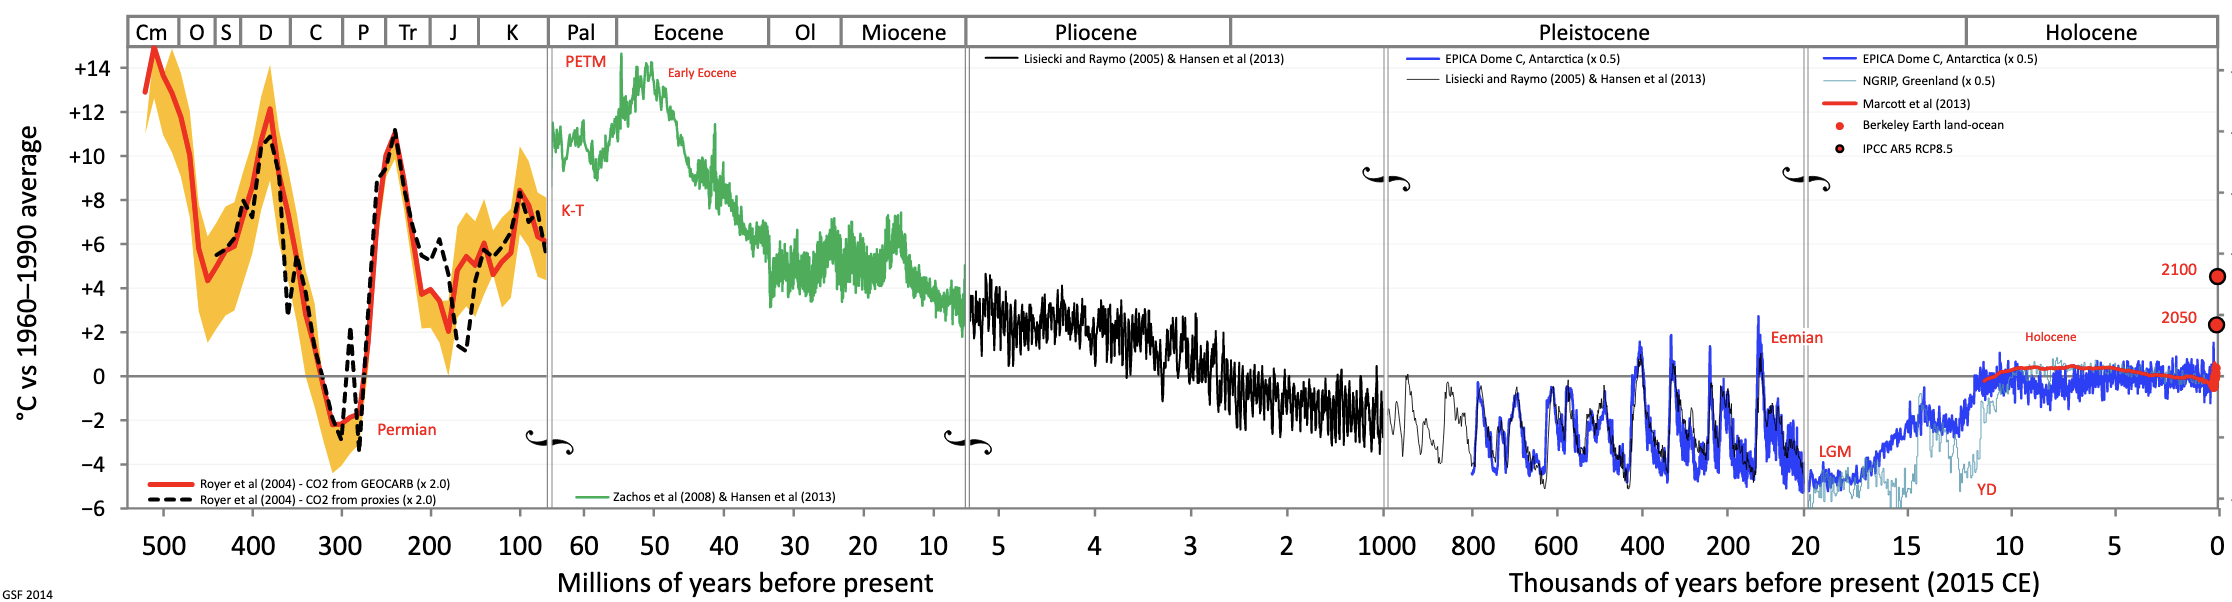
\includegraphics[width=\textwidth]{./Bilder/Paleoklima_Wiki.png}
\caption{\label{fig_PaleoTemp}%
Globale Durchschnittstemperatur auf der Erde w\"ahrend der letzten 540 Millionen Jahre.
Als Referenztemperatur dient die Durchschnittstemperatur zwischen 1960 und 1990. 
PETM: Pal\"aoz\"an/Eoz\"an-Temperaturmaximum; \glqq Permian\grqq\ bezieht sich auf
ein gro\ss es Massensterben von Pflanzen und Tieren, das vermutlich mit vulkanischen
Aktivit\"aten in Sibirien und einem vergleichsweise raschen Klimawandel einherging; \glqq Eemian\grqq\
bezieht sich auf die letzte Warmzeit (die Eem-Warmzeit) vor der letzten Kaltzeit; LGM: 
\glqq last glacial maximum\grqq\ bezeichnet das Maximum der letzten Kaltzeit; YD: \glqq
Younger Dryas\grqq, die J\"ungere Dryaszeit bezeichnet eine kurze K\"alteperiode, nachdem
die letzte Kaltzeit beendet war und ein Temperaturanstieg eingesetzt hatte; das Holoz\"an
ist die momentane Serie bzw.\ Epoche, die nach der letzten Kaltzeit einsetzte. (aus \cite{Wiki_Paleo})}
\end{figure}    

Man erkennt aber auch, dass es (z.B.\ vor rund 300 Millionen Jahren) schon mal 
K\"alteperioden\index{Eiszeit}\index{Kaltzeit}\index{Warmzeit}
gab, die mit unserer Eiszeit vergleichbar waren.\footnote{Nach der wissenschaftlichen Terminologie leben
wir heute in einer Eiszeit bzw.\ einem Eiszeitalter, wohingegen das, was wir umgangssprachlich als Eiszeit bezeichnen, 
nochmals als Kaltzeit (glacial) innerhalb einer Eiszeit gilt. Wir leben heute in einer Warmzeit (interglacial) 
innerhalb einer Eiszeit.
Die Definition von Eiszeitalter richtet sich danach, ob polare Regionen gro\ss fl\"achig vereist sind, wobei
manche Definitionen nur eine vereiste Region erfordern -- wir leben dann seit rund 34 Millionen Jahren
in einer Eiszeit -- w\"ahrend andere verlangen, dass Nord- und S\"udpol gro\ss fl\"achige 
Vereisungen zeigen -- danach leben wir seit 2,6 Millionen Jahren in einer Eiszeit.} Es gibt die Theorie
der \glqq Schneeballerde\grqq\ (snowball earth), wonach\index{Schneeballerde} 
insbesondere vor rund 600-700 Millionen Jahren die
Erde extreme K\"alteperioden durchgemacht hat, bei denen gro\ss e Teile der Erde (umstritten ist, ob
m\"oglicherweise die gesamte Erde, einschlie\ss lich vollst\"andig zugefrorener Ozeane) unter einer
Eisdecke lagen. 

\subsection{Proxies}

Proxies sind \glqq Stellvertreter\grqq. In der Pal\"aoklimatologie\index{Proxy} 
bezeichnen sie Parameter, die heute
bestimmt werden k\"onnen (z.B.\ das Verh\"altnis von ${}^{18}{\rm O}$ zu ${}^{16}{\rm O}$-Isotopen in
Gesteinsproben oder Fossilien) und von denen man gute Gr\"unde hat anzunehmen, dass sie
mit relevanten Parametern in der Vergangenheit korreliert sind (in diesem Fall z.B.\ mit der Oberfl\"achentemperatur
der Meere). 

Die Aufzeichnung bestimmter Parameter wie\index{Atmosph\"are!CO2@${\rm CO}_2$-Gehalt} 
Temperatur, ${\rm CO}_2$-Gehalt der Atmosph\"are, 
Solarkonstante etc.\ mit wissenschaftlichen Instrumenten hat erst in j\"ungerer Zeit begonnen. 
Daher erhebt sich die Frage, woher wir wissen (oder zu wissen glauben), welche Temperatur 
(${\rm CO}_2$-Gehalt, Methangehalt, Solarkonstante, etc) die Erde vor vielen Tausend bzw.\
Millionen Jahren hatte. Wenige Parameter k\"onnen wir mehr oder weniger direkt bestimmen:
Beispielsweise k\"onnen wir aus Eisbohrungen in der Antarktis in eingeschlossenen Luftblasen
direkt den ${\rm CO}_2$-Gehalt zu bestimmten vergangenen Zeiten in der Antarktis bestimmen. Auch andere
Parameter im Zusammenhang mit der chemischen Zusammensetzung der Luft lassen sich so bestimmen. 
Diese Messungen reichen maximal 800\,000 Jahre zur\"uck. Die meisten Parameter in weit
zur\"uckliegenden Zeiten werden jedoch indirekt gemessen. 

Typische Proxies sind bzw.\ finden sich in: Baumringen, Eisbohrkernen, Korallen, Ozeansedimenten, Fossilien, 
Gesteinsproben, etc.
Die folgenden Abschnitte sind nur Beispiele. Es gibt unz\"ahlige Proxies und in den meisten F\"allen
ist die Beziehung zwischen den heute gemessenen Werten und dem Parametern, auf die in fr\"uheren 
Zeiten geschlossen wird, sehr komplex. Die folgende Liste ist daher nur eine exemplarische
Auswahl. 

\subsubsection{Meeresoberfl\"achentemperatur (SST -- sea surface temperature)}

\begin{enumerate}
\item
$\delta {}^{18}{\rm O}$ ist ein Ma\ss\ f\"ur das\index{deltaO@$\delta {}^{18}{\rm O}$}\index{Meeresoberfl\"achentemperatur} 
Verh\"altnis von ${}^{18}{\rm O}$- zu\index{SST -- Sea Surface Temperature} 
${}^{16}{\rm O}$-Sauerstoffisotopen in unterschiedlichen Materialien. Definiert ist dieses 
Verh\"altnis durch
\begin{equation}
                            \delta {}^{18}{\rm O} = \frac{\Delta {\rm O}}{\Delta {\rm O}_{\rm St}} - 1 \, ,
\end{equation}
wobei $\Delta {\rm O} = \frac{{}^{18}{\rm O}}{{}^{16}{\rm O}}$ das Verh\"altnis von ${}^{18}{\rm O}$-Isotopen
zu ${}^{16}{\rm O}$-Isotopen in einer Probe ist und $\Delta {\rm O}_{\rm St}$ ein Standardwert f\"ur dieses
Verh\"altnis (definiert zu $1/498,7$, siehe \cite{Wiki_Vienna_Standard}). 

Das Isotop ${}^{18}{\rm O}$ ist schwerer als das Isotop ${}^{16}{\rm O}$. Daher verdunsten Wassermolek\"ule,
die das Isotop ${}^{18}{\rm O}$ enthalten, etwas schlechter als Wassermolek\"ule mit dem Isotop
${}^{16}{\rm O}$. F\"ur Oberfl\"achenmeerwasser in den Tropen ist das Verh\"altnis von
Wassermolek\"ulen mit ${}^{18}{\rm O}$ zu solchen mit ${}^{16}{\rm O}$ im Vergleich zu einem Standard
gr\"o\ss er. Regenwasser sowie Gebirgsb\"ache enthalten mehr ${}^{16}{\rm O}$. Diese Verh\"altnisse
h\"angen von der Temperatur ab und daher bildet $\delta {}^{18}{\rm O}$ ein Proxy f\"ur
die Oberfl\"achentemperatur von Wasser. 

Dies macht sich an manchen
Sedimenten bemerkbar. Insbesondere beobachtet man aber auch unterschiedliche Verh\"altnisse
in den karbonathaltigen Schalen bei sogenannten\index{Foraminiferen} 
Foraminiferen -- Mikroorganismen in Gew\"assersedimenten --, 
je nachdem welche Wassertemperatur 
zum jeweiligen Zeitpunkt der Schalenbildung herrschte. Das sogenannte Benthan (benthic) $\delta {}^{18}{\rm O}$ 
(Benthan, bzw.\ Englisch benthic, bezieht sich auf die obersten Schichten eines Gew\"assers) ist eines der wichtigsten
Proxies bei der Bestimmung von Temperaturen in vergangenen Zeiten.

\"Ahnliche Verh\"altnisse werden auch f\"ur\index{deltaN@$\delta {}^{15}{\rm N}$}\index{deltaC@$\delta {}^{13}{\rm C}$} 
andere Isotope definiert, beispielsweise $\delta {}^{15}{\rm N}$
(dem Isotopenverh\"altnis von ${}^{15}{\rm N}$ zu ${}^{14}{\rm N}$) und $\delta {}^{13}{\rm C}$
(dem Verh\"altnis von ${}^{13}{\rm C}$ zu ${}^{12}{\rm C}$). Diese Isotopenverh\"altnisse geben 
beispielsweise Aufschluss \"uber den Stickstoffgehalt in der Atmosph\"are oder von Wasser bzw.\
dem Methangehalt in der Atmosph\"are. 

\item
TEX${}_{86}$ steht\index{TEX${}_{86}$} 
f\"ur \glqq Tetraeder-Index von 86 Kohlenstoffatomen\grqq\  und ist eine Methode zur
Bestimmung von Meeresoberfl\"achentemperaturen in fr\"uheren Zeiten.  

Bestimmte mikroskopische Meeresorganismen (sogenannte mesophile marine Thaumarchaeota) 
besitzen eine Zellmembran, in denen sich sogenannte Glycerol-Dialkyl-Glycerol-Tetraethern-Molek\"ule 
-- GDGTs -- befinden. Diese Molek\"ule besitzen eine unterschiedliche Anzahl von Cyclopentyl-Komponenten,
das sind Ringe mit 5 C-Atomen. Die Anzahl dieser 5er-Ringe (typischer Weise zwischen 0 und 4) bzw.\ die
Mengenverh\"altnisse der GDGTs zu verschiedenen Ringzahlen h\"angen
von der Oberfl\"achentemperatur des Meeres zu dem Zeitpunkt ab, 
als sich diese Organismen gebildet haben, und dienen somit als Proxy f\"ur die Meeresoberfl\"achentemperatur. 
\end{enumerate}

\subsubsection{Sonnenaktivit\"at}

Proxies f\"ur die Sonnenaktivit\"at sind die Verh\"altnisse von ${}^{10}{\rm Be}$-Isotopen und
${}^{14}{\rm C}$-Isotopen zu ihren 
Standardisotopen.\index{Proxy!Sonnenaktivit\"at}\index{14-C@${}^{14}C}\index{10-Be@${}^{10}Be} 
Wie schon erw\"ahnt entstehen diese Isotope haupts\"achlich durch die kosmische Strahlung
in der Atmosph\"are der Erde. Der Einfluss der kosmischen Strahlung h\"angt wiederum
von der Sonnenaktivit\"at ab: Je h\"oher die Sonnenaktivit\"at, umso intensiver sind die Sonnenwinde,
die wiederum die kosmische Strahlung von der Erde teilweise ablenken. Je h\"oher die
Sonnenaktivit\"at, umso geringer ist die Intensit\"at der kosmischen Strahlung in den oberen 
Atmosph\"arenschichten und entsprechend geringer ist die Produktion von ${}^{10}{\rm Be}$-Isotopen und
${}^{14}{\rm C}$-Isotopen in diesen Schichten. Die Schwankungen in diesen Isotopen l\"asst sich
in verschiedenen Substanzen nachweisen und gibt daher einen Aufschluss \"uber die
Sonnenaktivit\"at in vergangenen Jahrtausenden bzw.\ Jahrmillionen. 

\subsubsection{Niederschlagsmengen und Sonnenscheindauer}

Die Niederschlagsmengen -- die Menge und H\"aufigkeit von Regenwasser -- hat einen Einfluss
auf die Stalagmiten in Tropfsteinh\"ohlen:\index{Niederschlagsmenge!Proxy}\index{Stalagmiten} 
Je h\"oher die Niederschlagsmenge umso mehr 
Wasser tr\"agt zur Bildung der Stalagmiten bei und umso breiter sind die B\"ander, die als
eine Form von \glqq Jahresringen\grqq\ beobachtet werden k\"onnen. 
Zumindest f\"ur die\index{Jahresringe}
letzten paar Tausend Jahre kann man so die Niederschlagsmengen eines Jahres
rekonstruieren. 

Ein anderes Proxy f\"ur die Niederschlagsmenge bzw.\ die Sonnenscheindauer in einem
Jahr sind die Jahresringe in alten B\"aumen. Auch bei manchen Schalentieren (Schnecken, Muscheln)
kann man aus den Ringstrukturen in den Schalen R\"uckschl\"usse auf das Wetter oder auch
andere Wachstumsbedingungen ziehen.
Solche Ringstrukturen findet man teilweise auch in Fossilien, sodass man Proxies aus sehr
weit zur\"uckliegenden Zeiten der Erdgeschichte hat. 

\subsubsection{Kohlendioxid-, Stickstoff- und Methangehalt in der Atmosph\"are}

F\"ur die vergangenen 800\,000 Jahre lassen sich die ${\rm CO}_2$-, ${\rm N}_2$- und
${\rm CH}_4$-Konzentrationen in der\index{Atmosph\"are!CO2@${\rm CO}_2$-Gehalt} 
Atmosph\"are mehr oder weniger direkt aus\index{CO2@${\rm CO}_2$-Gehalt!in fr\"uheren Zeiten}
Eiskernbohrungen in der Antarktis bestimmen (siehe Abb.\ \ref{fig_CO2}).

\begin{figure}[htb]
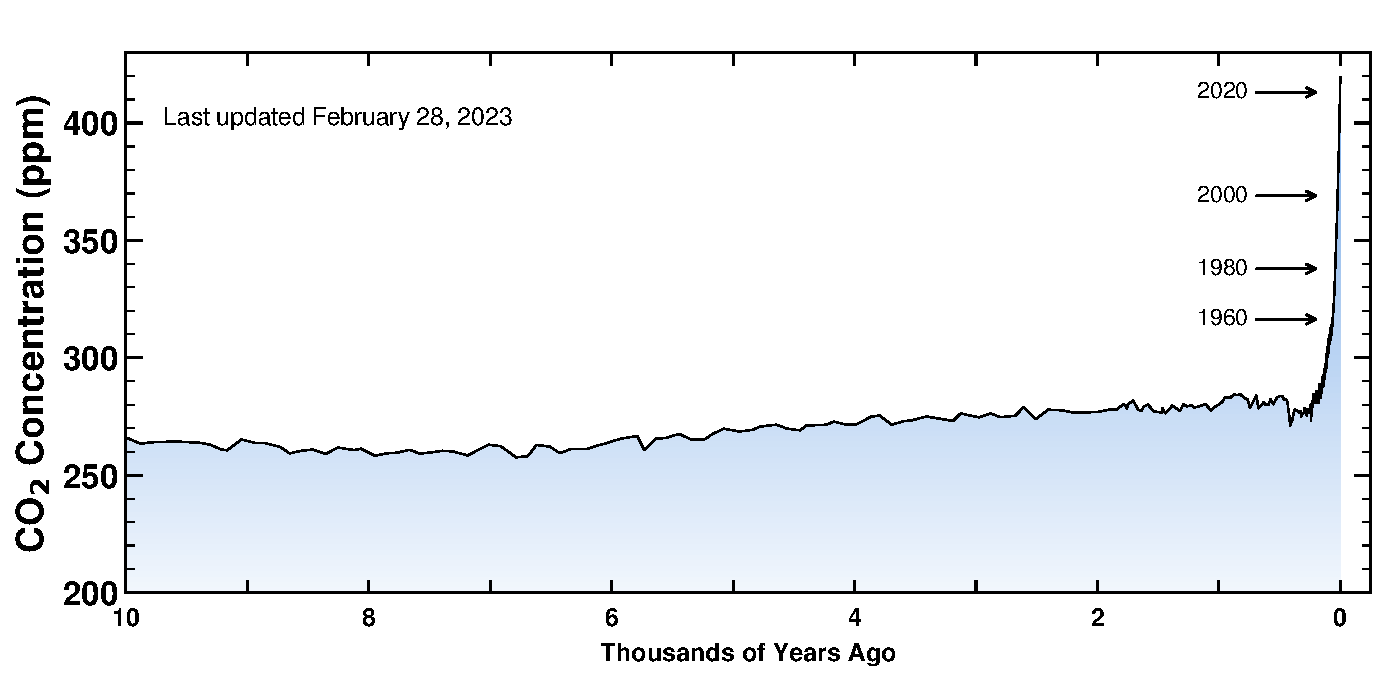
\includegraphics[width=0.49\textwidth]{./Bilder/co2_10k.pdf}
\hfill
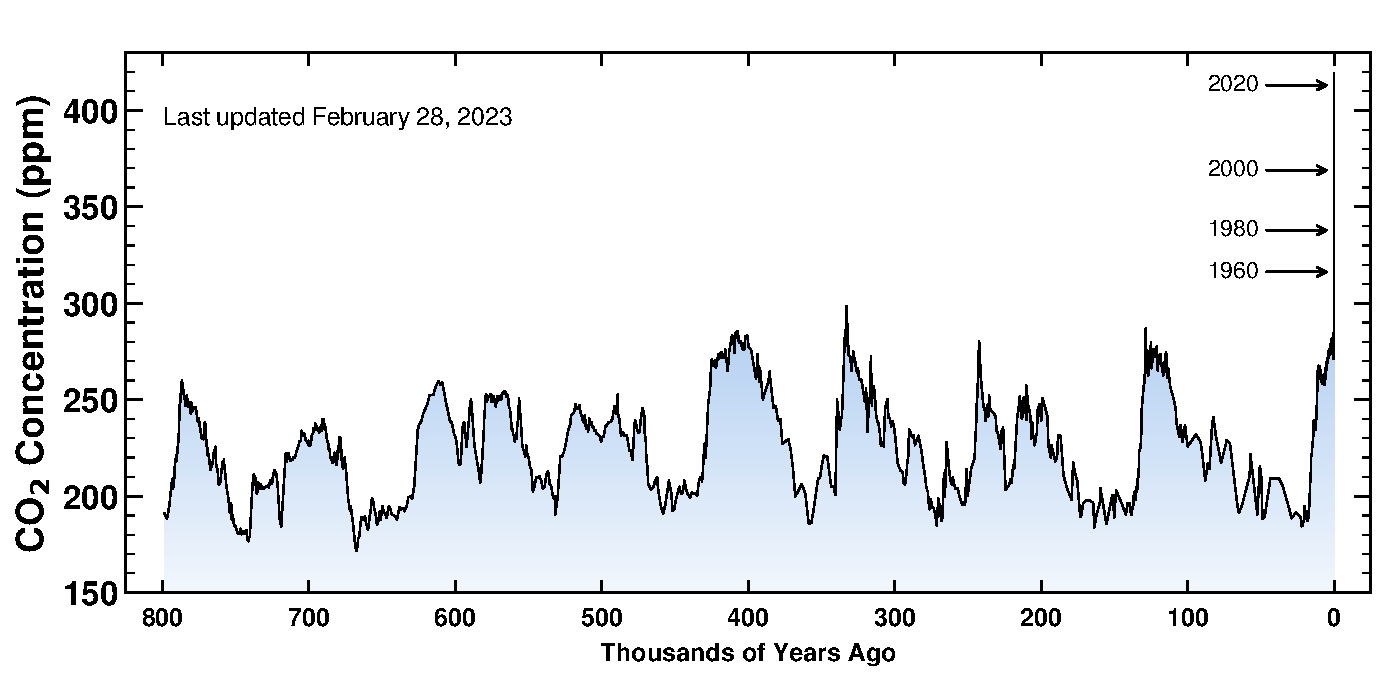
\includegraphics[width=0.49\textwidth]{./Bilder/co2_800k.pdf}
\caption{\label{fig_CO2}%
Der ${\rm CO}_2$-Gehalt in der Atmosph\"are, bestimmt aus Eiskernbohrungen in der
Antarktis. (links) f\"ur die vergangenen 10\,000 Jahre, (rechts) f\"ur die vergangenen
800\,000 Jahre.}
\end{figure} 

Man erkennt auf diesen Bildern sehr gut die sogenannte Hockeyschl\"agerkurve der
${\rm CO}_2$-Konzentration in den letzten 10\,000 Jahren nach der letzten Kaltzeit sowie
die Schwankungen zwischen Kaltzeiten und Warmzeiten innerhalb der letzten
800\,000 Jahre. Mit etwas Phantasie
erkennt man auch einen leichten Anstieg der ${\rm CO}_2$-Konzentrationen vor rund
6--8 Tausend Jahren, der mit dem Beginn von Viehzucht, Ackerbau und generell der
Sesshaftigkeit des Menschen einhergeht: Es wurden Weide- und Ackerbaufl\"achen 
abgebrannt und somit erste fossile Brennstoffe freigesetzt. Au\ss erdem haben beispielsweise
der Anbau von Reis auf gro\ss fl\"achigen Reisterrassen sowie die Viehzucht
die Freisetzung von Methan, einem weiteren Treibhausgas, gef\"ordert. Dieser Trend hat jedoch
lediglich dazu gef\"uhrt, dass eine einsetzende neue Kaltzeit etwas verz\"ogert wurde. 
Erst der Beginn der industriellen Revolution und der damit verbundene intensive Verbrauch
fossiler Brennstoffe vor rund 200 Jahren hat den ${\rm CO}_2$-Gehalt der Luft deutlich
ansteigen lassen. 

\section{Der Meeresspiegel} 

Eine\index{Meerespiegel!Proxy}\index{Meeresspiegel!in fr\"uheren Zeiten} 
der drastischsten Folgen eines Klimawandels ist der Anstieg des Meeresspiegels. 
Auch hier gibt es nat\"urlich viele Untersuchungen \"uber den Meeresspiegel in der
Vergangenheit. Beispielsweise war der Meerespiegel w\"ahrend der letzten Kaltzeiten
um rund 120 Meter niedriger als heute (siehe Abb.\ \ref{fig_PaleoSea}).

\begin{SCfigure}[30][htb]
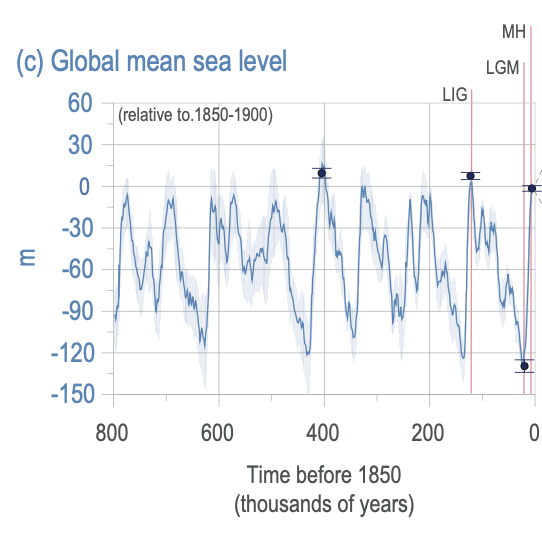
\includegraphics[width=0.4\textwidth]{./Bilder/Paleo_Sea_Level.png}
\caption{\label{fig_PaleoSea}%
Der mittlere Meerespiegel in den letzten 800\,000 Jahren relativ zu der
Zeitperiode 1850--1900. Deutlich erkennbar ist, dass der Meeresspiegel 
w\"ahrend der Kaltzeiten um \"uber 100 Meter niedriger war als heute. Allerdings war
der Meeresspiegel w\"ahrend der letzten Warmzeiten auch teilweise einige
Meter h\"oher. LIG last interglacial, LGM last glacial maximum, MH mid-Holocene.
(aus \cite{IPCC_WG1_AR6})}
\end{SCfigure}

Allerdings war er w\"ahrend der letzten Warmzeiten auch einige Meter
h\"oher als heute. Im Wesentlichen sind zwei Faktoren f\"ur die H\"ohe des 
Meeresspiegels verantwortlich: (1) die Temperatur des Wassers und (2) die
Menge an landgebundenem Eis. Die Temperatur des Wassers hat einen
Einfluss auf die Ausdehnung. Der Volumenausdehnungskoeffizient von Wasser
bei $20^\circ$C betr\"agt ungef\"ahr $\gamma = 0,2 \cdot 10^{-3} {\rm K}^{-1}$. Eine 
Wassers\"aule von 4\,000\,m (durchschnittliche Tiefe des Ozeans) w\"urde sich
bei einer Erw\"armung um 1 Grad Celsius somit um rund 80\,cm ausdehnen. 
Das gibt eine Vorstellung von der Gr\"o\ss enordnung. Nat\"urlich erw\"armt sich
das Wasser nicht gleich bis in eine Tiefe von 4\,km, andererseits betr\"agt die
langfristige Erw\"armung an der Oberfl\"ache vermutlich mehr als ein Grad. 

Der zweite
Faktor ist entscheidender: Da die Gesamtwassermenge an der Erdoberfl\"ache (Ozeane,
Land und Atmosph\"are) ungef\"ahr konstant ist, sinkt der Meeresspiegel,
wenn gro\ss e Landstriche (Antarktis, Gr\"onland, Alaska und Kanada, Nordeuropa,
etc.) mit Eis bedeckt sind. Bei der letzten Kaltzeit war Europa bis zu den Alpen mit
einer dicken Eisschicht bedeckt. Dies macht den gr\"o\ss ten Anteil der Schwankungen
in der Meeresh\"ohe aus. Schwimmendes Eis, wie es teilweise in der Arktis vorliegt, hat
aufgrund des archimedischen Prinzips
nat\"urlich keinen Einfluss auf die Wasserh\"ohe, 

Als Proxy f\"ur die Meereh\"ohe dienen oftmals bestimmte Fossilien im Sediment bzw.\
in Gesteinsproblem, von denen bekannt ist, dass sie nur in seichtem Meerwasser
leben. 

Die Pal\"aoklimatologie zeigt somit, dass wir in der Vergangenheit
sehr unterschiedliche klimatische Verh\"altnisse auf der Erde hatten. Man kann kaum
irgendein Klima als \glqq f\"ur die Erde normal\grqq\ bezeichnen. Einen wesentlichen Einfluss
hatten dabei die Kontinentalverschiebungen: Diese f\"uhrten zu ver\"anderten Str\"omungsverh\"altnissen
der Ozeane, zu teilweise erh\"ohten vulkanischen Aktivit\"aten mit massivem ${\rm CO}_2$ Aussto\ss, zum
Aufbau von Gebirgen wie dem Himalaya (bei diesen Prozessen werden gro\ss e Mengen
an ${\rm CO}_2$ durch Verwitterungsprozesse gebunden), etc. Ein weiterer Faktor waren
gro\ss e Meteoriteneinschl\"age, die in der fernen Vergangenheit h\"aufiger stattfanden als heute. 

Der Einfluss des Menschen\index{Klimawandel!anthropogener}
in j\"ungerer Zeit ist mittlerweile unbestritten. Letztendlich wird der anthropogene Klimawandel
den Planten Erde nicht zerst\"oren -- die Evolution wird neue, dem Klima angepasste Lebensformen
hervorbringen -- aber wir zerst\"oren den Lebensraum, in dem wir Menschen entstanden sind
und gleichzeitig werden viele vertraute Lebensformen aussterben, die im Zuge der k\"uhleren
letzten 20--30 Millionen Jahre entstanden sind. Viele derzeit bewohnte Gebiete werden im
Meer versinken und die H\"aufigkeit von Trockenzeiten und anderen extremen Wetterverh\"altnissen
werden zunehmen. Die Folgen des gr\"o\ss ten Problems -- die mit dem Klimawandel verbundene
Migration von Milliarden von Menschen -- sind dabei derzeit kaum absehbar. 
 

\section{Anmerkungen}

\begin{anmerkungen}
\item
\label{Anm-1}%
Der Grund f\"ur den Faktor 2 zwischen der Schwankung im Abstand und
der Schwankung in der Intensit\"at der Sonneneinstrahlung liegt in dem $1/r^2$-Gesetz
der Intensit\"at als Funktion des Abstands:
\begin{equation}
        \frac{1}{(r\pm \Delta r)^2} \approx \frac{1}{r^2} \mp 2 \frac{\Delta r}{r} \, .
\end{equation}

\end{anmerkungen}



\begin{thebibliography}{99}
\bibitem{ICS} International Commission on Stratigraphy (ICS) \url{https://stratigraphy.org/chart}. 
\bibitem{IPCC_WG1_AR6} IPCC -- Climate Change 2021; The Physical Science Basis, 
            Full Report, Working Group I Contribution to the Sixth Assessment Report (S.\,159). 
\bibitem{NASA_World} NASA Image and Video Library, 
       \url{https://images.nasa.gov/details/as17-148-22727}
\bibitem{NASA_facts} NASA Earth Fact Sheet; 
      \url{https://nssdc.gsfc.nasa.gov/planetary/factsheet/earthfact.html}   
\bibitem{Solar} Solarkonstante; Uni Kassel,\\
       \url{https://www.greenrhinoenergy.com/solar/radiation/images/solar-constant.jpg}         
\bibitem{Wikipedia_Faint} Wikipedia \glqq Faint young Sun paradox\grqq\ 
        \url{https://en.wikipedia.org/wiki/Faint_young_Sun_paradox}.                 
\bibitem{Wikipedia_Milankovic} Wikipedia \glqq Milankovitch cycles\grqq.   
       \url{https://en.wikipedia.org/wiki/Milankovitch_cycles}.      
\bibitem{Wiki_Paleo} Wikipedia \glqq Paleoclimatology\grqq\ \url{https://en.wikipedia.org/wiki/Paleoclimatology}.         
\bibitem{Wikipedia_Solarkonstante} Wikipedia \glqq Solarkonstante\grqq.   
       \url{https://de.wikipedia.org/wiki/Solarkonstante}.    
\bibitem{Wiki_Vienna_Standard} Wikipedia \glqq Vienna Standard Mean Ocean
         Water\grqq\ \url{https://de.wikipedia.org/wiki/Vienna_Standard_Mean_Ocean_Water}.                  
\end{thebibliography}

\end{document}


\documentclass[german,10pt]{book}      
\usepackage{makeidx}
\usepackage{babel}            % Sprachunterstuetzung
\usepackage{amsmath}          % AMS "Grundpaket"
\usepackage{amssymb,amsfonts,amsthm,amscd} 
\usepackage{mathrsfs}
\usepackage{rotating}
\usepackage{sidecap}
\usepackage{graphicx}
\usepackage{color}
\usepackage{fancybox}
\usepackage{tikz}
\usetikzlibrary{arrows,snakes,backgrounds}
\usepackage{hyperref}
\hypersetup{colorlinks=true,
                    linkcolor=blue,
                    filecolor=magenta,
                    urlcolor=cyan,
                    pdftitle={Overleaf Example},
                    pdfpagemode=FullScreen,}
%\newcommand{\hyperref}[1]{\ref{#1}}
%
\definecolor{Gray}{gray}{0.80}
\DeclareMathSymbol{,}{\mathord}{letters}{"3B}
%
\newcounter{num}
\renewcommand{\thenum}{\arabic{num}}
\newenvironment{anmerkungen}
   {\begin{list}{(\thenum)}{%
   \usecounter{num}%
   \leftmargin0pt
   \itemindent5pt
   \topsep0pt
   \labelwidth0pt}%
   }{\end{list}}
%
\renewcommand{\arraystretch}{1.15}                % in Formeln und Tabellen   
\renewcommand{\baselinestretch}{1.15}                 % 1.15 facher
                                                      % Zeilenabst.
\newcommand{\Anmerkung}[1]{{\begin{footnotesize}#1 \end{footnotesize}}\\[0.2cm]}
\newcommand{\comment}[1]{}
\setlength{\parindent}{0em}           % Nicht einruecken am Anfang der Zeile 

\setlength{\textwidth}{15.4cm}
\setlength{\textheight}{23.0cm}
\setlength{\oddsidemargin}{1.0mm} 
\setlength{\evensidemargin}{-6.5mm}
\setlength{\topmargin}{-10mm} 
\setlength{\headheight}{0mm}
\newcommand{\identity}{{\bf 1}}
%
\newcommand{\vs}{\vspace{0.3cm}}
\newcommand{\noi}{\noindent}
\newcommand{\leer}{}

\newcommand{\engl}[1]{[\textit{#1}]}
\parindent 1.2cm
\sloppy

         \begin{document}  \setcounter{chapter}{2}


\chapter{Physik des Klimas III\\Klimamodelle}
% Kap x
\label{chap_Klima3}

F\"ur das Verst\"andnis unseres Klimas sowie die M\"oglichkeiten, Vorhersagen zu treffen, wie sich
unser Klima in den n\"achsten Jahrzehnten entwickeln wird und wie wir die Auswirkungen eines
Klimawandels, der mittlerweile kaum noch bestritten wird, m\"oglichst gering halten k\"onnen,
spielen Klimamodelle eine wichtige Rolle. Es sind auch gerade die Aussagen solcher Klimamodelle,
die von Leugnern eines anthropogenen (d.h.\ vom Menschen verursachten) Klimawandels immer
wieder in Frage gestellt werden. Daher ist es wichtig, einen ungef\"ahren Eindruck von Klimamodellen
zu bekommen. 

In diesem Kapitel betrachten wir zun\"achst sehr einfache Klimamodelle, die sich auf den globalen 
Energiehaushalt der Erde beziehen. Insgesamt ist dieser Energiehaushalt
nahezu ausgeglichen. Au\ss erdem handelt es sich um statische Modelle, d.h., wir untersuchen  
die Gleichgewichtszust\"ande solcher Modelle und wie sich diese ver\"andern, wenn sich \"au\ss ere
Parameter ver\"andern. Gegen Ende dieses Kapitels beschreiben wir auch kurz die wichtigsten
Modelle, die heute f\"ur Klimaprognosen verwendet werden. Die Modelle lassen sich kaum noch
in ihrer Komplexit\"at \"uberschauen, aber man kann zumindest grob beschreiben, welche Effekte
von diesen Modellen ber\"ucksichtigt werden. 

\section{Grundlagen}

F\"ur die einfachen Klimamodelle, die hier besprochen werden, sind die folgenden Grundlagen
relevant. Ausf\"uhrlicher wird auf diese Themen in Kap.\ \ref{chap_Klima1} eingegangen. 

\subsection{Die Solarkonstante}

Die Solarkonstante ist definiert als das langj\"ahrige Mittel der Intensit\"at der 
Sonneneinstrahlung oberhalb der Erdatmosph\"are. 
Die Intensit\"at ist dabei die Energie, die pro Sekunde 
auf eine bestimme Fl\"ache - in diesem Fall ein Quadratmeter senkrecht zur Strahlungsrichtung - trifft
(siehe Kap.\ \ref{chap_Klima1}). 
Die IAU (International Astronomical Union) hat 2015 die Solarkonstante aufgrund neuerer
Messungen auf den Wert
\begin{equation}
               S = 1361\,{\rm J \cdot s^{-1} \cdot m^{-2}} = 1361\,{\rm W \cdot m}^{-2}  
\end{equation}
festgelegt.

Auf Zeitskalen von einigen hundert Jahren liegt die dominante Schwankung der Solarkonstante in
den 11-j\"ahrigen Aktivit\"atszyklen der Sonne. Diese wirken sich aber im sichtbaren Bereich
kaum aus. Die beobachteten Schwankungen in der Temperatur im langj\"ahrigen Mittel aufgrund
dieser Sonnenzyklen liegt in der Gr\"o\ss enordnung von $0,1^\circ$C. Zum Einfluss l\"angerfristiger
Schwankungen (z.B.\ der sogenannten Milankovi\'c-Zyklen), siehe Kap.\ \ref{chap_Klima1}

\subsection{Die Albedo}

Einen wesentlich gr\"o\ss eren Einfluss auf das Klima hat die Albedo
der Erde (siehe Kap.\ \ref{chap_Klima1}). Hierbei handelt es sich um die Reflektivit\"at der
Erde f\"ur den Wellenl\"angenbereich der Sonnenstrahlung. Je gr\"o\ss er die Albedo, umso
gr\"o\ss er ist die Menge an Energie, die direkt wieder in den Weltraum abgegeben wird und
somit auf den Energiehaushalt der Erde keinen Einfluss hat. Derzeit liegt die Albedo der Erde
bei $a=0,3$, d.h.\ rund 30\% der eingestrahlten Energie wird entweder an den Wolken oder
der Erdoberfl\"ache zur\"uck in den Weltraum reflektiert. Den wichtigsten Beitrag zur Albedo der
Erde liefern neben den Wolken die Schnee- und Eisfl\"achen der n\"ordlichen und s\"udlichen
Breitengrade. Auch landschaftliche Ver\"anderungen, beispielsweise das Abholzen von Nadelw\"aldern
(die eine sehr kleine Albedo haben) und die Ersetzung durch Wiesen oder St\"adte, haben einen
Einfluss. Der weitaus gr\"o\ss te Unsicherheitsfaktor bei Klimamodellen sind die Wolken und die
damit zusammenh\"angende Albedo: Es ist bisher kaum verstanden, wie die Wolkendichte auf 
den Klimawandel reagieren wird.

\subsection{Aufbau der Erdatmosph\"are}

Ebenfalls wichtig f\"ur Klimamodelle ist der Aufbau der unteren Atmosph\"are. Bis zu einer
H\"ohe von rund 12--13\,km (in Poln\"ahe und im Winter ist diese Schicht etwas tiefer, in den
Tropen kann sie bis zu 18--20\,km betragen) reicht die Troposph\"are. In dieser Schicht spielt
sich unser Wettergeschehen ab. Definiert ist diese Schicht durch einen negativen
Temperaturgradienten, d.h.,\ die Temperatur nimmt in dieser Schicht mit zunehmender
H\"ohe ab. Den Haupteinfluss auf dieses Verhalten hat die Tatsache, dass sich aufsteigende Luftmassen,
deren Druck daher abnimmt, abk\"uhlen. Nimmt die Temperatur eines solchen Luftpakets mit der
H\"ohe nicht rasch genug ab, bleibt es w\"armer als die Umgebungstemperatur. Dadurch
steigt es weiter auf, da ein w\"armeres Luftpaket (bei gleichem Druck) weniger dicht und damit
leichter ist. Auf diese Weise
kommt es zur Konvektion: Warme Luftschichten steigen auf, k\"uhlen
sich dabei ab, je nach Luftfeuchtigkeit sinkt die Temperatur unter den sogenannten Taupunkt -
hier kommt es zur Kondensation von Wasser und Wolkenbildung. Bei der Kondensation wird
Energie frei, die den Auftrieb der Luftmassen nochmals beschleunigt. 

Oberhalb der Troposph\"are liegt die Stratosph\"are, die bis in eine H\"ohe von rund 50\,km
reicht. Hier nimmt die Temperatur mit der H\"ohe wieder zu, von rund $(-50)^\circ-(-80)^\circ$C
(abh\"angig von der Jahreszeit und dem Breitengrad)
bis wieder zum Gefrierpunkt von $0^\circ$C. Der Grund daf\"ur ist, dass sich in dieser Schicht
die Ozonschicht der Erde befindet. Diese absorbiert ultraviolette Sonnenstrahlung und erw\"armt
sich dadurch. Die weiteren Schichten (Mesosph\"are, Thermosph\"are
und Exosph\"are) spielen f\"ur das Klima eine untergeordnete Rolle.

Die Luft der Atmosph\"are besteht im Wesentlichen aus Stickstoff (${\rm N}_2$, rund 78\%) und
Sauerstoff (${\rm O}_2$, rund 21\%) sowie dem Edelgas Argon (${\rm Ar}$, rund $0,9$\%). 
Der Rest sind Spurengase, deren Anteile meist in ppm (parts per million), ppb (parts per billion)
oder ppt (parts per trillion) angegeben werden. Hierbei handelt es sich um Volumenanteile, also
im Wesentlichen Anteile pro Teilchenzahl, da wir bei Gasen (insbesondere Gasen, die sich wie
ideale Gase verhalten) das Eigenvolumen der Molek\"ule vernachl\"assigen k\"onnen. 
${\rm CO}_2$ (Kohlendioxid) ist mit derzeit rund 420\,ppm
oder $0,042$\% das h\"aufigste Gas, es folgen Ne (Neon, 18\,ppm), He (Helium, 5\,ppm),
${\rm CH}_4$ (Methan, 1870\,ppb). Au\ss erdem enth\"alt die Luft je nach Luftfeuchtigkeit bis zu 
4 Volumenprozent ${\rm H_2O}$ (Wasserdampf).

\section{Einige globale, statische Klimamodelle}

Ein Klimamodell ist ein System mathematischer Gleichungen, in das klimarelevante
Parameter (z.B.\ Luft- und Wassertemperatur in bestimmten Luftschichten bzw.\
Wassertiefen, Niederschl\"age, Luftfeuchtigkeit, 
Eisfl\"ache und Dicke von Eisschichten, ... eventuell ortsabh\"angig) eingehen und das
den zeitlichen Verlauf solcher Parameter beschreibt. Die einfachsten Klimamodelle betrachten
lediglich die Durchschnittstemperatur der Erde (also keine Ortsabh\"angigkeiten). Weitere
Vereinfachungen bestehen darin, die Zeitabh\"angigkeit zu vernachl\"assigen, d.h., es werden
Gleichgewichtszust\"ande untersucht. Selbst auf diesem Niveau unterscheiden sich
Klimamodelle noch hinsichtlich der Eigenschaften der Erdoberfl\"ache, die ber\"ucksichtigt werden.

Die folgenden Klimamodelle sind von dieser globalen Struktur und ber\"ucksichtigen zunehmend
mehr Einfl\"usse. Man erkennt, wie schnell die Modell komplexer werden, wie andererseits
aber auch einfache Modelle schon bestimmte nicht-triviale Effekte beschreiben k\"onnen. 
Abbildung \ref{fig_Bilanz} gibt global die Strahlungsbilanz der Atmosph\"are wieder, die 
n\"aherungsweise in den angef\"uhrten Modellen beschrieben wird.

\begin{SCfigure}[30][htb]
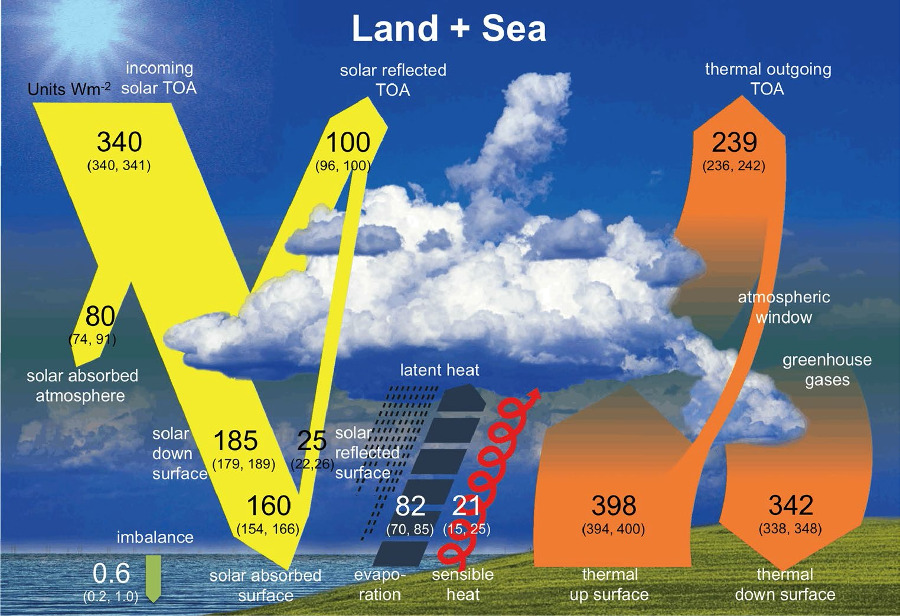
\includegraphics[scale = 0.3]{./Bilder/Bilanz.jpg}
\caption{\label{fig_Bilanz}%
Einfaches Diagramm zur Veranschaulichung des radiativen Energiehaushalts
der Atmosph\"are. TOA = top of atmosphere. Die Zahlen bezeichnen eine
Strahlungsintensit\"at (in Watt pro Quadratmeter). In Klammern ist jeweils
das Intervall der Unsicherheit angegeben. (Aus \cite{Sanchez})} 
\end{SCfigure}

Im Folgenden verwenden wir auch das Kirchhoff'sche Strahlungsgesetz, wonach der
Absorptionskoeffizient und der Emissionskoeffizient eines K\"orpers gleich sind. Wir setzen
hier die integrierte diffuse Strahlung voraus, d.h.\ wir betrachten keine Richtungsabh\"angigkeiten. 
Allerdings ber\"ucksichtigen einige der Klimamodelle eine Frequenzabh\"angigkeit dieser
Koeffizienten. Die Interpretation sogenannter Emissionskoeffizienten in diesem Kapitel
bedeutet meist, dass die Atmosp\"are f\"ur bestimmte Frequenzen
absorbierend und f\"ur andere Frequenzen durchl\"assig ist. Daher ist die Forderung, dass
die frequenzabh\"angige Absorbtion gleich der entsprechenden Emission ist, eher eine
N\"aherung. 


\subsection{Klimamodell 1 - ohne Atmosph\"are}

Wir betrachten zun\"achst ein sehr einfaches Klimamodell, bei dem folgende Faktoren
ber\"ucksichtigt werden:
\begin{enumerate}
\item
eine konstante Intensit\"at der Sonnenstrahlung oberhalb der Atmosph\"are, dies ist die Solarkonstante 
$S=1\,361\,{\rm J\cdot s^{-1} \cdot m^{-2}}$,
\item
eine konstante Albedo von $a=0,3$,
\item
eine Erdoberfl\"ache, welche die absorbierte Energie in alle Richtungen als
Schwarzk\"orperstrahlung entsprechend ihrer Oberfl\"achentemperatur $T$ abgibt. 
Hier wird das Stefan-Boltzmann-Gesetz 
\begin{equation}
                L=\sigma T^4
\end{equation}                 
angenommen, d.h., die abgestrahlte Intensit\"at $L$ (Energie pro Zeit und Fl\"ache) ist 
proportional zur 4.\ Potenz der
absoluten Temperatur $T$ der Erdoberfl\"ache.
Die Proportionalit\"atskonstante ist die Stefan-Boltzmann-Konstante
$\sigma = 5,67 \cdot 10^{-8}\,{\rm J \cdot {s}^{-1} \cdot m^{-2} \cdot K^{-4}}$.\hyperref[Anm-2]{(2)}  
\end{enumerate}
Bis auf die Oberfl\"achentemperatur der Erde sind alle Parameter bekannt. F\"ur die
gesamte Intensit\"at der absorbierten Strahlung gilt:
\begin{equation}
          L_{\rm ab} = (1 - a ) S \pi R^2 \, .
\end{equation}
Der Faktor $(1-a)$ beschreibt die Reduktion der eingestrahlten Intensit\"at $S$ aufgrund
der Albedo. $\pi R^2$ (wobei $R$ der Radius der Erde ist) beschreibt die Querschnittsfl\"ache
der Erde, die von der Sonnenstrahlung getroffen wird. Meist argumentiert man, dass dies die
Fl\"ache des Schattens hinter der Erde ist, wo die Sonnenstrahlung fehlt, weil sie auf die
Erde getroffen ist. 

Diese absorbierte Intensit\"at muss im Gleichgewicht gleich der emittierten Intensit\"at
sein (siehe Abb.\ \ref{fig_Klima1}). 
Bei der emittierten Intensit\"at soll es sich in diesem Modell um die Intensit\"at der
Schwarzk\"orperstrahlung der Erde bei ihrer Oberfl\"achentemperatur
$T_{\rm s}$ handeln (siehe Abb.\ \ref{fig_Klima1}, (a)):
\begin{equation}
         L_{\rm em} = \sigma T_{\rm s}^4 \, 4 \pi R^2 \, .
\end{equation}
Hier wird als emittierende Fl\"ache die gesamte Oberfl\"ache der Erde angenommen (daher
der Faktor 4). Setzt man $L_{\rm ab}=L_{\rm em}$ folgt
\begin{equation}
      (1-a) S = 4 \sigma T_{\rm s}^4 \hspace{1cm} \Longrightarrow \hspace{1cm}
          T_{\rm s} = \sqrt[4]{\frac{(1-a) S}{4 \sigma}} = 254,6\,{\rm K} \, .
\end{equation}
Nach diesem einfachen Modell m\"usste die durchschnittliche Erdtemperatur knapp 255\,K oder 
$- 18^\circ$C betragten. Das ist nat\"urlich viel zu kalt. Bei diesen Temperaturen w\"aren die
Ozeane gefroren. Die tats\"achliche Jahresdurchschnittstemperatur der Erde liegt (2017) bei $15^\circ$C
oder 288\,K. 

\begin{figure}[htb]
\begin{tikzpicture}
\draw (0,1) -- (7,1);
\filldraw[fill=gray!20] (0,1) -- (7,1) -- (7,0) -- (0,0) -- (0,1);
\draw (2.0,5) -- (2.0,2) -- (1.7,2) -- (2.5,1) -- (3.3,2) -- (3.0,2) -- (3.0,5);
   \draw (4.0,1.1) -- (4.0,4) -- (3.7,4) -- (4.5,5) -- (5.3,4) -- (5.0,4) -- (5.0,1.1);
\draw [->,snake=snake, segment amplitude = 0.4mm, segment length = 2mm,
               line after snake=1mm] (0,5) -- (1,1.2);
\draw [->,snake=snake, segment amplitude = 0.4mm, segment length = 2mm,
               line after snake=1mm] (0.4,5) -- (1.4,1.2);
\draw [->,snake=snake, segment amplitude = 0.4mm, segment length = 4mm,
               line after snake=1mm] (5.6,1.2) -- (6.6,5);
\draw [->,snake=snake, segment amplitude = 0.4mm, segment length = 4mm,
               line after snake=1mm] (6,1.2) -- (7,5);
\draw (3.5,0.5) node {$T_{\rm S}$};
\draw (3.5,5) node {(a)};
\draw (2,3) node {$L_{\rm ab}=\frac{(1-a)S}{4}$};
\draw (5,3) node {$L_{\rm em}=\sigma T_{\rm s}^4$};
\end{tikzpicture}
\hspace{1cm} %
\begin{tikzpicture}
\draw (0,1) -- (7,1);
\filldraw[fill=gray!20] (0,1) -- (7,1) -- (7,0) -- (0,0) -- (0,1);
\draw (2.0,5) -- (2.0,2) -- (1.7,2) -- (2.5,1) -- (3.3,2) -- (3.0,2) -- (3.0,5);
   \draw (4.0,1.1) -- (4.0,4) -- (3.7,4) -- (4.5,5) -- (5.3,4) -- (5.0,4) -- (5.0,1.1);
\draw [->,snake=snake, segment amplitude = 0.4mm, segment length = 2mm,
               line after snake=1mm] (0,5) -- (1,1.2);
\draw [->,snake=snake, segment amplitude = 0.4mm, segment length = 2mm,
               line after snake=1mm] (0.4,5) -- (1.4,1.2);
\draw [->,snake=snake, segment amplitude = 0.4mm, segment length = 4mm,
               line after snake=1mm] (5.6,1.2) -- (6.6,5);
\draw [->,snake=snake, segment amplitude = 0.4mm, segment length = 4mm,
               line after snake=1mm] (6,1.2) -- (7,5);
\draw (3.5,5) node {(b)};
\draw (3.5,0.5) node {$T_{\rm s}$};
\draw (2,3) node {$L_{\rm ab}=\frac{(1-a)S}{4}$};
\draw (5,3) node {$L_{\rm em}=\hat{\epsilon} \sigma T_{\rm s}^4$};
\end{tikzpicture}
\caption{\label{fig_Klima1}%
Zwei einfache Klimamodelle. (a) In diesem Modell wird s\"amtliche von der Sonne einfallende
Strahlung (abz\"uglich der Albedo) 
von der Erdoberfl\"ache absorbiert und von dieser als Schwarzk\"orperstrahlung wieder
in den Weltraum abgegeben. (b) In diesem Modell gibt die Erdoberfl\"ache ebenfalls alle absorbierte 
Strahlung wieder ab, allerdings nicht als Schwarzk\"orperstrahlung sondern um einen
Faktor $\hat{\epsilon}$ geringer. Dieser Faktor beschreibt den Einfluss des Treibhauseffekts, 
gibt aber keine Erkl\"arung.}
\end{figure}

\subsection{Klimamodell 2 - ohne Atmosph\"arenschicht, mit Emissionsfaktor}

Es gibt mehrere Gr\"unde, weshalb das erste Klimamodell eine deutlich zu tiefe
Oberfl\"achentemperatur der Erde liefern k\"onnte. Zum Einen
k\"onnte es eine Energiequelle geben, die bisher nicht ber\"ucksichtigt wurde. Daf\"ur
kommt praktisch nur die Erde selbst in Frage, insbesondere die Kernzerf\"alle im Inneren
der Erde. Hier zeigt eine genauere \"Uberlegung jedoch, dass dieser Effekt zu klein ist und
f\"ur die Klimabetrachtungen nicht ber\"ucksichtigt zu werden braucht.  

Weiterhin k\"onnte die Annahme falsch sein, dass die Erde eine Schwarzk\"orperstrahlung
zu einer Temperatur $T$ abgibt, die ihrer Oberfl\"achentemperatur entspricht. Wir f\"uhren f\"ur
unser zweites Klimamodell einen Emissionsfaktor $\hat{\epsilon}$ ein, setzen also f\"ur die
emittierte Intensit\"at
\begin{equation}
         L_{\rm em} = \hat{\epsilon} \sigma T^4 \, 4 \pi R^2 
\end{equation}
an. $\hat{\epsilon}=1$ entspricht dem alten Modell. Man spricht in diesem Fall auch schon mal
von einem \glqq grauen Strahler\grqq\ (siehe Abb.\ \ref{fig_Klima1}(b)). Wir erhalten nun f\"ur die
Oberfl\"achentemperatur der Erde:
\begin{equation}
      (1-a) S = 4 \hat{\epsilon} \sigma T^4 \hspace{1cm} \Longrightarrow \hspace{1cm}
          T = \sqrt[4]{\frac{(1-a) S}{4 \hat{\epsilon} \sigma}} = \sqrt[4]{\frac{1}{\hat{\epsilon}}} ~ 254,6\,{\rm K} \, .
\end{equation}
Setzen wir f\"ur $T$ die beobachtete Oberfl\"achentemperatur von 288\,K ein, erhalten
wir $\hat{\epsilon} = 0,61$. Wir haben an dieser Stelle unser \glqq Klimamodell\grqq\ nicht zur
Bestimmung der Oberfl\"achentemperatur $T$ benutzt, sondern zur Bestimmung von
$\hat{\epsilon}$. Gelegentlich wird behauptet, der niedrigere Wert von $\hat{\epsilon}$ beschreibe 
den Treibhauseffekt. Das ist zwar nicht falsch, bedarf aber einer Erkl\"arung. 
Inwieweit $\hat{\epsilon}$ direkt gemessen und somit aus diesem Modell die
Oberfl\"achentemperatur der Erde bestimmt werden kann, werden wir noch
diskutieren. 

\subsection{Klimamodell 3 - eine total absorbierende Atmosph\"arenschicht}

Wir betrachten nun ein Modell, bei dem zwischen der einfallenden Strahlung,
die durch die Solarkonstante gegeben ist, und der ausfallenden Strahlung, die in
den bisherigen beiden Modellen durch die Temperatur der Erdoberfl\"ache
gegeben ist, noch eine Schicht liegt, welche den Einfluss der Treibhausgase
beschreiben soll. Diese Schicht sei vollkommen durchl\"assig f\"ur die einfallende
(kurzwellige) Strahlung der Sonne, sie absorbiere aber die langwellige Strahlung zur Temperatur $T_{\rm s}$,
die von der Erde emittiert wird. Au\ss erdem emittiere sie eine langwellige Strahlung zu ihrer
Atmosph\"arentemperatur $T_{\rm a}$ (siehe Abb.\ \ref{fig_Klima2}). Diese Emission erfolgt
sowohl in Richtung Weltraum (nach oben) als auch zur\"uck in Richtung Erdoberfl\"ache.
Wir haben es nun also mit zwei Temperaturen zu tun: einmal die Temperatur
der Erdoberfl\"ache $T_{\rm s}$ sowie weiterhin die Temperatur $T_{\rm a}$ der Atmosph\"arenschicht,
die wir uns als sehr d\"unn denken. 
 
\begin{SCfigure}[30][htb]
\begin{tikzpicture}
\draw (0,1) -- (9,1);
\filldraw[fill=gray!20] (0,1) -- (9,1) -- (9,0) -- (0,0) -- (0,1);
\filldraw[fill=gray!20] (0,3) -- (2,3) -- (2,2.5) -- (0,2.5) -- (0,3);
\filldraw[fill=gray!20] (3,3) -- (9,3) -- (9,2.5) -- (3,2.5) -- (3,3);
\draw (2.0,5) -- (2.0,2) -- (1.7,2) -- (2.5,1) -- (3.3,2) -- (3.0,2) -- (3.0,5);
\draw (4.5,1.0) -- (4.5,1.5) -- (4.2,1.5) -- (5.0,2.5) -- (5.8,1.5) -- (5.5,1.5) -- (5.5,1.0);
\draw (6.5,2.5) -- (6.5,1.5) -- (6.3,1.5) -- (6.8,1) -- (7.3,1.5) -- (7.1,1.5) -- (7.1,2.5);
\draw (5.7,3.0) -- (5.7,4.5) -- (5.5,4.5) -- (6.0,5) -- (6.5,4.5) -- (6.3,4.5) -- (6.3,3.0);
\draw [->,snake=snake, segment amplitude = 0.4mm, segment length = 2mm,
               line after snake=1mm] (0,5) -- (1,1.1);
\draw [->,snake=snake, segment amplitude = 0.4mm, segment length = 2mm,
               line after snake=1mm] (0.4,5) -- (1.4,1.1);
\draw [->,snake=snake, segment amplitude = 0.4mm, segment length = 4mm,
               line after snake=1mm] (7.6,1.1) -- (8.0,2.6);
\draw [->,snake=snake, segment amplitude = 0.4mm, segment length = 4mm,
               line after snake=1mm] (8,1.1) -- (8.4,2.6);
\draw [->,snake=snake, segment amplitude = 0.4mm, segment length = 4mm,
               line after snake=1mm] (8.3,2.9) -- (8.7,5);
\draw [->,snake=snake, segment amplitude = 0.4mm, segment length = 4mm,
               line after snake=1mm] (8.5,2.6) -- (8.7,1.1);
\draw (4.5,0.5) node {$T_{\rm s}$};
\draw (6.5,0.5) node {Erdboden};
\draw (4.5,2.75) node {$T_{\rm a}$};
\draw (6.5,2.75) node {Atmosph\"are};
\draw (2.0,4) node {$L_{\rm ab}=\frac{(1-a)S}{4}$};
\draw (4.8,1.9) node {$L_{\rm em}=\sigma T_{\rm s}^4$};
\draw (6.8,1.9) node {$L_{\rm a}=\sigma T_{\rm a}^4$};
\draw (6.2,3.9) node {$L_{\rm a}=\sigma T_{\rm a}^4$};
\draw (9.5,0) node {~}; 
\end{tikzpicture}
%\hspace{1cm} %
\caption{\label{fig_Klima2}%
Der Treibhauseffekt - Klimamodell mit einer Atmosph\"arenschicht. Die von der Erdoberfl\"ache
emittierte langwellige Strahlung wird in der Atmosph\"are absorbiert und als
Schwarzk\"orperstrahlung zur Atmosph\"arentemperatur $T_a$ sowohl in
den Weltraum als auch zur\"uck zur Erdoberfl\"ache emittiert.}
\end{SCfigure}

F\"ur beide Schichten - Erdoberfl\"ache und Atmosph\"are - stellen wir nun
Bilanzgleichungen auf. Dabei nehmen wir an, dass die Atmosph\"are nur Energie
von der Erdoberfl\"ache erh\"alt, die entsprechend dem Stefan-Boltzmann-Gesetz
durch $L_{\rm em}=\sigma T_{\rm S}^4$ gegeben ist. Au\ss erdem emittiere die
Atmosph\"are die Energie in zwei Richtungen - nach oben und nach unten - 
entsprechend ihrer Temperatur $T_{\rm a}$. Wir erhalten somit die folgenden zwei
Bilanzgleichungen ((s) f\"ur \glqq surface\grqq, d.h.\ die Bilanzgleichung des Erdbodens,
und (a) f\"ur die Bilanzgleichung der Atmosph\"arenschicht):
\begin{equation}
            (s) \hspace{0.5cm}  \frac{(1-a)}{4} S  +  \sigma T_{\rm a}^4 = \sigma T_{\rm s}^4 \hspace{2cm}
            (a) \hspace{0.5cm}  \sigma T_{\rm s}^4  = 2 \sigma T_{\rm a}^4 \, .
\end{equation}
Bilanzgleichung ($s$) beschreibt die Strahlungsbilanz der Erdoberfl\"ache: Einfallend 
(linke Seite der Gleichung) ist die
kurzwellige Strahlung der Sonne sowie ein Teil, der von der Atmosph\"are nach unten emittiert wird;
ausfallend ist die langwellige Strahlung, welche die Erdoberfl\"ache entsprechend ihrer
Temperatur $T_{\rm s}$ emittiert. Bilanzgleichung ($a$)
beschreibt die Strahlungsbilanz der Atmosph\"arenschicht (die als d\"unn und von konstanter Temperatur
angenommen wird): Einfallend ist die emittierte langwellige Strahlung der Erde, emittiert werden
zwei Anteile (nach unten und nach oben in den Weltraum) entsprechend der Temperatur $T_{\rm a}$.

Aus der zweiten Gleichung folgt unmittelbar $T_{\rm s} = \sqrt[4]{2}\, T_{\rm a}$, die Temperatur der
Erdoberfl\"ache ist also um den Faktor $\sqrt[4]{2} \approx 1,1892$ h\"oher als die Temperatur $T_{\rm a}$ der
Atmosph\"are. Setzt man die zweite Bilanzgleichung in die erste ein, erh\"alt man f\"ur die Atmosph\"arentemperatur
den Wert des ersten Modells $T_{\rm a} \approx 254,6$\,K oder $-18^\circ$C. Dies ist auch plausibel, weil f\"ur das
Gesamtsystem die Strahlungsbilanz ebenfalls ausgeglichen sein soll. F\"ur die Temperatur der Erdoberfl\"ache
erhalten wir nun $T_{\rm s}\approx 303$\,K oder $30^\circ$C. Das ist etwas zu warm wenn man bedenkt, dass die
mittlere Temperatur der Erdoberfl\"ache eher bei $15^\circ$C liegt. 

An diese Modell wird offensichtlich, dass die Temperatur, die man aus einer gro\ss en Entfernung von der
Erde beobachtet, nicht die Temperatur der Erdoberfl\"ache ist (wie in dem ersten Modell), sondern die
Temperatur der (oberen) Atmosph\"arenschicht. 

\subsection{Klimamodell 4 - eine teilabsorbierende Atmosph\"arenschicht}

\begin{SCfigure}[30][htb]
\begin{tikzpicture}
\draw (0,1) -- (9,1);
\filldraw[fill=gray!20] (0,1) -- (9,1) -- (9,0) -- (0,0) -- (0,1);
\filldraw[fill=gray!20] (0,3) -- (2,3) -- (2,2.5) -- (0,2.5) -- (0,3);
\filldraw[fill=gray!20] (3,3) -- (3.7,3) -- (3.7,2.5) -- (3,2.5) -- (3,3);
\filldraw[fill=gray!20] (4.1,3) -- (9,3) -- (9,2.5) -- (4.1,2.5) -- (4.1,3);
\draw (2.0,5) -- (2.0,2) -- (1.7,2) -- (2.5,1) -- (3.3,2) -- (3.0,2) -- (3.0,5);
\draw (4.7,1.0) -- (4.7,1.5) -- (4.4,1.5) -- (5.1,2.5) -- (5.8,1.5) -- (5.5,1.5) -- (5.5,1.0);
\draw (3.7,1.0) -- (3.7,4) -- (3.5,4) -- (3.9,5) -- (4.3,4) -- (4.1,4) -- (4.1,1.0);
\draw (6.5,2.5) -- (6.5,1.5) -- (6.3,1.5) -- (6.8,1) -- (7.3,1.5) -- (7.1,1.5) -- (7.1,2.5);
\draw (5.7,3.0) -- (5.7,4.5) -- (5.5,4.5) -- (6.0,5) -- (6.5,4.5) -- (6.3,4.5) -- (6.3,3.0);
\draw [->,snake=snake, segment amplitude = 0.4mm, segment length = 2mm,
               line after snake=1mm] (0,5) -- (1,1.1);
\draw [->,snake=snake, segment amplitude = 0.4mm, segment length = 2mm,
               line after snake=1mm] (0.4,5) -- (1.4,1.1);
\draw [->,snake=snake, segment amplitude = 0.4mm, segment length = 4mm,
               line after snake=1mm] (7.6,1.1) -- (8.6,5.0);
\draw [->,snake=snake, segment amplitude = 0.4mm, segment length = 4mm,
               line after snake=1mm] (7.8,1.1) -- (8.2,2.6);
\draw [->,snake=snake, segment amplitude = 0.4mm, segment length = 4mm,
               line after snake=1mm] (8,1.1) -- (8.4,2.6);
\draw [->,snake=snake, segment amplitude = 0.4mm, segment length = 4mm,
               line after snake=1mm] (8.3,2.9) -- (8.8,5);
\draw [->,snake=snake, segment amplitude = 0.4mm, segment length = 4mm,
               line after snake=1mm] (8.5,2.6) -- (8.7,1.1);
\draw (4.5,0.5) node {$T_{\rm s}$};
\draw (6.5,0.5) node {Erdboden};
\draw (5.0,2.75) node {$T_{\rm a}$};
\draw (6.5,2.75) node {Atmosph\"are};
\draw (2.0,4) node {$L_{\rm ab}=\frac{(1-a)S}{4}$};
\draw (4.3,3.8) node {$L_{\rm em}=$};
\draw (4.1,3.4) node {$(1-\epsilon) \sigma T_{\rm s}^4$};
\draw (5.1,1.9) node {$L_{\rm em}=\epsilon \sigma T_{\rm s}^4$};
\draw (7.0,1.9) node {$L_{\rm a}=\epsilon \sigma T_{\rm a}^4$};
\draw (6.5,4.2) node {$L_{\rm a}=\epsilon \sigma T_{\rm a}^4$};
\draw (9.5,0) node {~}; 
\end{tikzpicture}
%\hspace{1cm} %
\caption{\label{fig_Klima3}%
Effektiver Treibhauseffekt mit einer teilweise absorbierenden
Atmosph\"arenschicht. Die von der Erdoberfl\"ache
emittierte langwellige Strahlung wird teilweise in der Atmosph\"are absorbiert 
und teilweise durchgelassen. Der absorbierte Anteil wird als \glqq graue Strahlung\grqq\
mit Emissionskoeffizienten $\epsilon$ zur Atmosph\"arentemperatur $T_a$ sowohl in
den Weltraum als auch zur\"uck zur Erdoberfl\"ache emittiert.}
\end{SCfigure}

In diesem Klimamodell wird angenommen, dass die Atmosph\"arenschicht nur einen Teil
der von der Erde emittierten langwelligen Strahlung absorbiert (parametrisiert durch den Parameter $\epsilon$)
und einen Teil direkt durchl\"asst (siehe Abb.\ \ref{fig_Klima3}). Entsprechend den
Kirchhoff'schen Strahlungsgesetzen, wonach Absorptions- und Emissionskoeffizient eines
K\"orpers f\"ur eine gegebene Wellenl\"ange gleich sind (Richtungsabh\"angigkeiten werden hier
vernachl\"assigt), wird bei
diesem Modell angenommen, dass die Atmosph\"are f\"ur bestimmte Wellenl\"angen
transparent ist - und entsprechend bei diesen Wellenl\"angen auch nicht emittiert - 
und andere Wellenl\"angen absorbiert, die dann auch wieder (diffus, also in alle Richtungen) emittiert werden. 

Nun lauten die Bilanzgleichungen:
\begin{equation}
            (s) \hspace{0.5cm}  \frac{(1-a)}{4} S  + \epsilon \sigma T_{\rm a}^4 
                = ((1-\epsilon) + \epsilon) \sigma T_{\rm s}^4 = \sigma T_{\rm s}^4 \hspace{1.8cm}
            (a) \hspace{0.5cm}  \epsilon \sigma T_{\rm s}^4  = 2 \epsilon \sigma T_{\rm a}^4 \, .
\end{equation}
Aus der zweiten Gleichung (f\"ur die Atmosph\"arenschicht) folgt:
\begin{equation}
                 T^4_{\rm s} = 2 \, T^4_{\rm a}  \hspace{1cm} {\rm bzw.} \hspace{1cm}  
                 T_{\rm s} = \sqrt[4]{2} ~ T_{\rm a}  \, .  
\end{equation}
Wenn wir dies in die erste Gleichung einsetzen, erhalten wir f\"ur die Atmosph\"arentemperatur:
\begin{equation}
           T_{\rm a} = \sqrt[4]{\frac{(1-a)S}{4} \frac{1}{2-\epsilon}}
                                =  \sqrt[4]{\frac{1}{2-\epsilon}} ~ 254,6\,{\rm K} 
\end{equation}
und damit f\"ur die Bodentemperatur der Erde:
\begin{equation}
           T_{\rm s} = \sqrt[4]{\frac{(1-a)S}{4} \frac{2}{2-\epsilon}}
                                =  \sqrt[4]{\frac{2}{2-\epsilon}}  ~  254,6\,{\rm K} \, .
\end{equation}
F\"ur $\epsilon \rightarrow 0$ erhalten wir unser erstes Modell wieder: Die Atmosph\"are
emittiert keine Strahlung mehr (ihre Temperatur w\"are $T_{\rm a} = (1/\sqrt[4]{2})\cdot 254,6$\,K
$\approx 214,1$\,K, bei der aber praktisch keine Strahlung emittiert wird). S\"amtliche von der Erdoberfl\"ache
absorbierte Energie wird als Schwarzk\"orperstrahlung bei $254,6$\,K wieder in den Weltraum 
abgestrahlt. F\"ur $\epsilon \rightarrow 1$ erhalten wir das vorherige Modell: Die Atmosph\"arentemperatur
betr\"agt $254,6$\,K und die Temperatur der Erdoberfl\"ache ist $T_{\rm s}=\sqrt[4]{2}\cdot 254,6\,{\rm K}
\approx 303$\,K. 

Wenn wir nun umgekehrt f\"ur die durchschnittliche Oberfl\"achentemperatur der Erde den Wert $288$\,K
annehmen, erhalten wir den Wert $\epsilon \approx 0,7785$, und f\"ur die Atmosph\"arentemperatur
folgt daraus ein Wert von rund $242$\,K. \"Uber Polareis (siehe Abb.\ \ref{fig_updown}) w\"urde sich f\"ur
eine Erdtemperatur von $268$\,K eine Atmosph\"arentemperatur von $226$\,K ergeben, was recht gut
mit den beobachteten Werten \"ubereinstimmt. Der Vorteil dieses Modells
ist, dass wir hier einige Effekte studieren und interpretieren k\"onnen, die bisher nicht so
offensichtlich waren.

\begin{SCfigure}[30][htb]
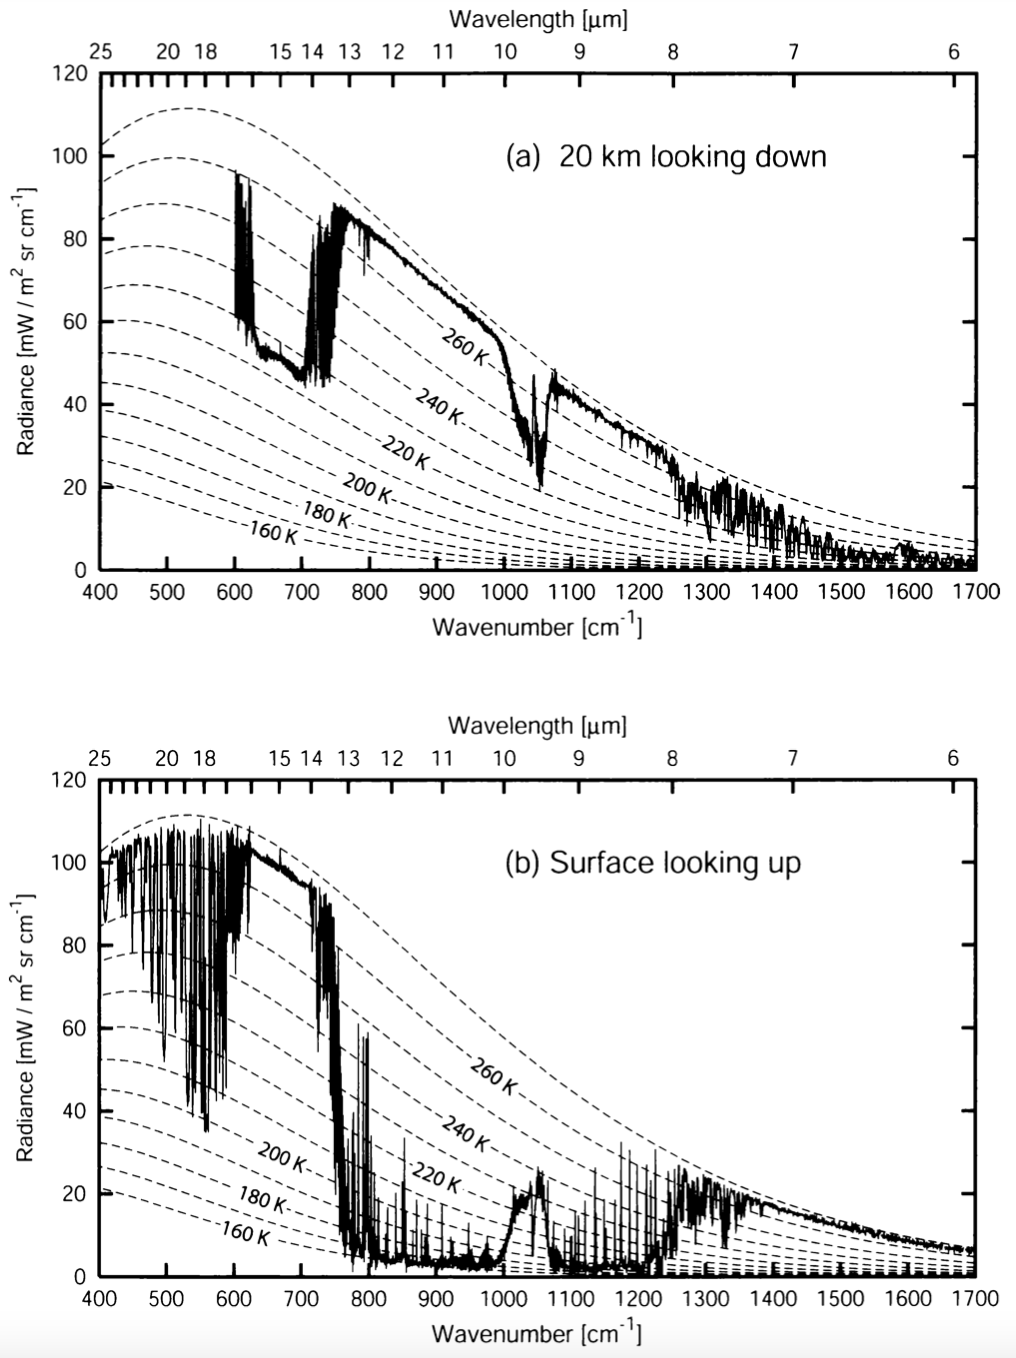
\includegraphics[scale = 0.4]{./Bilder/Petty.png}
\caption{\label{fig_updown}%
(oben) Spektralzerlegung der Erdstrahlung aus gro\ss er H\"ohe betrachtet.
(unten) Spektrale Zerlegung der Atmosph\"arenstrahlung vom Erdboden aus
betrachtet. Die Diagramme wurden \"uber Polareis aufgenommen. 
Die wellenl\"angenabh\"angigen Kurven werden verglichen mit
Schwarzk\"orperstrahlungen zu verschiedenen Temperaturen. Aus gro\ss er H\"ohe
sieht man Bereiche mit einer Temperatur von rund 268\,K - diese entsprechen
der Erdoberfl\"ache - und andere Bereiche mit einer Temperatur von rund 226\,K - 
diese entsprechen der oberen Atmosph\"are. In Wellenl\"angenbereichen, in denen
die Atmosph\"are lichtdurchl\"assig ist, sieht man im oberen Bild eine Temperatur von rund
268\,K, also den Erdboden, und im unteren Bild eine sehr niedrige Temperatur entsprechend
dem Weltraum. Aus \cite{Petty}.}  
\end{SCfigure}

\begin{enumerate}
\item
F\"ur $\epsilon \neq 1$ oder 0 entspricht die Strahlung, welche die Erde in den Weltraum
abgibt - die also von einer gro\ss en H\"ohe aus beobachtet wird - nicht einer
Schwarzk\"orperstrahlung zu einer festen Temperatur sondern einer Strahlung zu zwei
Temperaturen. Damit erh\"alt der Parameter $\hat{\epsilon}$ aus dem zweiten Modell eine
anschauliche Bedeutung: Bei manchen
Wellenl\"angen ist die Atmosph\"are durchl\"assig und man sieht somit bei diesen Wellenl\"angen aus 
gro\ss er H\"ohe die Oberfl\"ache der Erde (und ihre Temperatur). Bei anderen
Wellenl\"angen ist die Atmosph\"are absorbierend und undurchsichtig. Bei diesen Wellenl\"angen
sieht man aus einer gro\ss en H\"ohe nur die obere Atmosph\"arenschicht und dies bei einer
deutlich niedrigeren Temperatur (vgl.\ Abb.\ \ref{fig_updown}).
\item
Wenn $\epsilon$ gr\"o\ss er wird, also mehr Strahlung von der Atmosph\"are absorbiert wird,
nimmt die Temperatur der Erdoberfl\"ache zu. Dies ist der eigentliche Treibhauseffekt. 
Gleichzeitig nimmt in diesem Modell aber auch die Temperatur der oberen Atmosph\"arenschicht, von der
aus die Strahlung in den Weltraum abgegeben wird, zu. Sie ist allerdings insgesamt k\"alter
als in dem Klimamodell 3. Da die einfallende Intensit\"at
(die Solarkonstante und die Albedo) mehr oder weniger konstant bleibt, muss auch die
abgegebene Intensit\"at in der Summe konstant bleiben. Wenn aber von der Erdoberfl\"ache
Strahlung zu einer h\"oheren Temperatur in den Weltraum abgegeben wird, muss die Strahlung
von den oberen Atmosph\"arenschichten zu einer tieferen Temperatur geh\"oren.
\end{enumerate} 

\subsection{Ein einfaches Klimamodell f\"ur die Venus}

Die Atmosph\"are der Venus enth\"alt rund 96\% Kohlendioxid. Der Abstand Venus-Sonne
betr\"agt ungef\"ahr $0,72$\,AU (astronomische Einheiten) und somit ist die Solarkonstante
an der Oberfl\"ache der Venusatmosph\"are um rund das Inverse von $(0,72)^2 \approx 0,52$,
also knapp das Doppelte, gr\"o\ss er als 
auf der Erde (dies beruht auf dem $1/r^2$-Gesetz der Intensit\"at einer Strahlung als Funktion des
Abstands von der Strahlungsquelle). Allerdings ist die Albedo der Venus mit rund $0,75$ deutlich gr\"o\ss er als die
der Erde (von au\ss en erscheint die Venus vollkommen wolkenbedeckt). 
Insgesamt m\"usste es daher auf der Venus k\"alter sein, als auf der Erde. 
Doch die Oberfl\"achentemperatur der Venus betr\"agt \"uber $460^\circ$C. Um zu sehen, wie
eine dickere absorbierende Atmosph\"arenschicht die Oberfl\"achentemperatur beeinflusst,
betrachten wir folgendes Atmosph\"arenmodell (siehe Abb.\ \ref{fig_Klima4}). 

\begin{SCfigure}[30][htb]
\begin{tikzpicture}
%\draw (0,1) -- (9,1);
\filldraw[fill=gray!20] (0,1) -- (9,1) -- (9,0) -- (0,0) -- (0,1);
\filldraw[fill=gray!20] (0,3) -- (2,3) -- (2,2.5) -- (0,2.5) -- (0,3);
\filldraw[fill=gray!20] (3,3) -- (9,3) -- (9,2.5) -- (3,2.5) -- (3,3);
\filldraw[fill=gray!20] (0,5) -- (2,5) -- (2,4.5) -- (0,4.5) -- (0,5);
\filldraw[fill=gray!20] (3,5) -- (9,5) -- (9,4.5) -- (3,4.5) -- (3,5);
\draw (2.0,6) -- (2.0,2) -- (1.7,2) -- (2.5,1) -- (3.3,2) -- (3.0,2) -- (3.0,6);
\draw (4.5,1.0) -- (4.5,1.5) -- (4.2,1.5) -- (5.0,2.5) -- (5.8,1.5) -- (5.5,1.5) -- (5.5,1.0);
\draw (6.5,2.5) -- (6.5,1.5) -- (6.3,1.5) -- (6.8,1) -- (7.3,1.5) -- (7.1,1.5) -- (7.1,2.5);
\draw (4.8,3.0) -- (4.8,4.0) -- (4.6,4.0) -- (5.1,4.5) -- (5.6,4.0) -- (5.4,4.0) -- (5.4,3.0);
\draw (6.5,4.5) -- (6.5,3.5) -- (6.3,3.5) -- (6.7,3) -- (7.1,3.5) -- (6.9,3.5) -- (6.9,4.5);
\draw (5.8,5.0) -- (5.8,5.7) -- (5.6,5.7) -- (6,6.2) -- (6.4,5.7) -- (6.2,5.7) -- (6.2,5.0);
\draw [->,snake=snake, segment amplitude = 0.4mm, segment length = 2mm,
               line after snake=1mm] (0,6) -- (1,1.1);
\draw [->,snake=snake, segment amplitude = 0.4mm, segment length = 2mm,
               line after snake=1mm] (0.4,6) -- (1.4,1.1);
\draw [->,snake=snake, segment amplitude = 0.4mm, segment length = 4mm,
               line after snake=1mm] (7.6,1.1) -- (8.0,2.6);
\draw [->,snake=snake, segment amplitude = 0.4mm, segment length = 4mm,
               line after snake=1mm] (7.8,1.1) -- (8.2,2.6);
\draw [->,snake=snake, segment amplitude = 0.4mm, segment length = 4mm,
               line after snake=1mm] (8,1.1) -- (8.4,2.6);
\draw [->,snake=snake, segment amplitude = 0.4mm, segment length = 4mm,
               line after snake=1mm] (8.5,2.6) -- (8.7,1.0);
\draw [->,snake=snake, segment amplitude = 0.4mm, segment length = 4mm,
               line after snake=1mm] (7.9,2.9) -- (8.2,4.6);
\draw [->,snake=snake, segment amplitude = 0.4mm, segment length = 4mm,
               line after snake=1mm] (8.1,2.9) -- (8.4,4.6);
\draw [->,snake=snake, segment amplitude = 0.4mm, segment length = 4mm,
               line after snake=1mm] (8.5,4.6) -- (8.7,2.9);
\draw [->,snake=snake, segment amplitude = 0.4mm, segment length = 4mm,
               line after snake=1mm] (8.2,4.9) -- (8.4,6.2); 
\draw (4.5,0.5) node {$T_{\rm s}$};
\draw (6.5,0.5) node {Oberfl\"ache Venus};
\draw (4.5,2.75) node {$T_{\rm a1}$};
\draw (6.5,2.75) node {Atmosph\"are 1}; 
\draw (4.5,4.75) node {$T_{\rm a2}$};
\draw (6.5,4.75) node {Atmosph\"are 2};
\draw (2.0,4) node {$L_{\rm ab}=\frac{(1-a)S}{4}$};
\draw (4.8,1.9) node {$L_{\rm em}=\sigma T_{\rm s}^4$};
\draw (6.8,1.9) node {$L_{\rm a1}=\sigma T_{\rm a1}^4$};
\draw (5.0,3.7) node {$L_{\rm a1}=\sigma T_{\rm a1}^4$};
\draw (6.8,3.7) node {$L_{\rm a2}=\sigma T_{\rm a2}^4$};
\draw (6.0,5.4) node {$L_{\rm a2}=\sigma T_{\rm a2}^4$};
\draw (9.2,0) node {~}; 
\end{tikzpicture}
%\hspace{1cm} %
\caption{\label{fig_Klima4}%
Modell f\"ur den Treibhauseffekt der Venus - ein Klimamodell mit zwei Atmosph\"arenschichten. 
Die von der Venusoberfl\"ache
emittierte langwellige Strahlung wird in der ersten Atmosph\"are absorbiert und als
Schwarzk\"orperstrahlung zur Atmosph\"arentemperatur $T_{\rm a1}$ zur zweiten Schicht wie
auch zur\"uck zur Venusoberfl\"ache emittiert. Die zweite Schicht mit der Temperatur
$T_{\rm a2}$ emittiert Strahlung zur\"uck zur ersten Schicht und in den Weltraum.}
\end{SCfigure}

Die Bilanzgleichungen sind nun (wobei durch die Stefan-Boltzmann-Konstante $\sigma$ dividiert
wurde):
\begin{equation}
       (g) \hspace{0.5cm}   \frac{(1-a)S}{4\sigma} + T_{\rm a1}^4 = T_{\rm s}^4 
       \hspace{1cm} (a1) \hspace{0.5cm}   
        T_{\rm s}^4 + T_{\rm a2}^4 = 2  T_{\rm a1}^4 
       \hspace{1cm} (a2) \hspace{0.5cm}   
        T_{\rm a1}^4 = 2  T_{\rm a2}^4  \, 
\end{equation}
Aus diesen Gleichungen erhalten wir (die Zahlenwerte gelten zum besseren Vergleich mit den
vorherigen Modellen f\"ur die Albedo und die Solarkonstante der Erde):
\begin{eqnarray}
         T_{\rm a2} &=& \sqrt[4]{\frac{(1-a) S}{4 \sigma}} = 254,6\,{\rm K}  \\
         T_{\rm a1} &=& \sqrt[4]{2} T_{\rm a2} =  \sqrt[4]{2}\cdot
                                   \sqrt[4]{\frac{(1-a) S}{4 \sigma}} = \sqrt[4]{2}\cdot 254,6\,{\rm K} 
                                      \approx 302,8\, {\rm K} \\
         T_{\rm s} &=& \sqrt[4]{3} T_{\rm a2} 
                                =  \sqrt[4]{3} \cdot \sqrt[4]{\frac{(1-a) S}{4 \sigma}} = \sqrt[4]{3} \cdot 254,6\,{\rm K} 
                                      \approx 335,1\, {\rm K} 
\end{eqnarray}
Die oberste Atmosph\"arenschicht beh\"alt somit ihre Temperatur von $254,6$\,K, wohingegen die
Temperatur am Boden im Vergleich zu dem Einschicht-Modell nochmals gewachsen ist. Man kann
sich nun leicht \"uberlegen, dass sich dieses Verhalten bei mehreren Atmosph\"arenschichten fortsetzt. 
Letztendlich erh\"alt man, dass immer dieselbe Temperatur von $254,6$\,K in den Weltraum abgestrahlt
wird, diese Temperatur zu den tieferen Schichten hin zunimmt und am Boden theoretisch einen
beliebig hohen Wert annehmen kann. Auch wenn sich die Zahlenwerte hier auf die Albedo und die
Solarkonstante der Erde beziehen, kann man das Modell leicht auf Venus \"ubertragen. Durch die hohe
Konzentration an ${\rm CO}_2$ (sowie die Tatsache, dass die Atmosph\"are der Venus fast 90 mal
dichter ist als die der Erde)
wirken dort effektiv viele Atmosph\"arenschichten total absorbierend.

Modelle f\"ur die Atmosph\"aren anderer Planeten oder auch von Monden anderer Planeten (z.B.\ der
Jupiter- und Saturnmonde) sind auch f\"ur die Klimaphysik von Interesse, weil man an diesen
Modellen testen kann, ob die Zusammenh\"ange durch die einfachen Modelle schon nahezu korrekt
wiedergegeben werden und somit diese einfachen Modelle der Realit\"at entsprechen.

\subsection{Klimamodell 5 - Erw\"armung der Troposph\"are und Abk\"uhlung der Stratosph\"are}
\label{sec_Klima5}

Nun betrachten wir ein Klimamodell mit zwei Atmosph\"arenschichten, von denen
eine Schicht n\"aherungsweise die Verh\"altnisse in der Troposph\"are und eine zweite
Schicht die Verh\"altnisse in der Stratosph\"are beschreibt. Es ist das allgemeinste Modell in diesem
Kapitel und man erh\"alt alle vorherigen Modelle f\"ur spezielle Werte der Parameter. 

Die Stratosph\"are
zeichnet sich dadurch aus, dass sie einen Teil der einfallenden Sonnenstrahlung
absorbiert (insbesondere im UV-Bereich durch das in der Stratosph\"are vorhandene
Ozon) und in W\"arme umwandelt. Ansonsten wirken sowohl die Troposph\"are als
auch die Stratosph\"are als \glqq graue Strahler\grqq, die bestimmte Wellenl\"angen
absorbieren und emittieren und andere Wellenl\"angen transmittieren und in diesem
Bereich auch nicht emittieren (siehe Abb.\ \ref{fig_Klima5}). Die zugeh\"origen
Emissionsfaktoren (gleich Absorptionsfaktoren) $\epsilon_{\rm tro}$ und $\epsilon_{\rm str}$
geben wieder den Anteil einer Strahlung an, die von dieser Schicht absorbiert und
emittiert wird. 

\begin{figure}[htb]
\begin{tikzpicture}
%\draw (0,1) -- (9,1);
\filldraw[fill=gray!20] (0,1) -- (15,1) -- (15,0) -- (0,0) -- (0,1);         %  Erde
\filldraw[fill=gray!20] (0,3) -- (1.7,3) -- (1.7,2.5) -- (0,2.5) -- (0,3);    %    Trop 1
\filldraw[fill=gray!20] (2.7,3) -- (4.9,3) -- (4.9,2.5) -- (2.7,2.5) -- (2.7,3);   %  Trop  2
\filldraw[fill=gray!20] (5.9,3) -- (11.0,3) -- (11.0,2.5) -- (5.9,2.5) -- (5.9,3);   %  Trop  3
\filldraw[fill=gray!20] (11.4,3) -- (15,3) -- (15,2.5) -- (11.4,2.5) -- (11.4,3);  % Trop  4
\filldraw[fill=gray!20] (0,5) -- (1.7,5) -- (1.7,4.5) -- (0,4.5) -- (0,5);        %  Stra 1
\filldraw[fill=gray!20] (2.7,5) -- (5.5,5) -- (5.5,4.5) -- (2.7,4.5) -- (2.7,5);  %  Stra  2
\filldraw[fill=gray!20] (5.9,5) -- (8.6,5) -- (8.6,4.5) -- (5.9,4.5) -- (5.9,5);     %  Stra 3
\filldraw[fill=gray!20] (9.0,5) -- (15,5) -- (15,4.5) -- (9.0,4.5) -- (9.0,5);     %  Stra 4
\draw (1.7,6.5) -- (1.7,2) -- (1.4,2) -- (2.2,1) -- (3.0,2) -- (2.7,2) -- (2.7,5.8);    %  top -> s
\draw (2.7,5.3) -- (2.5,5.3) -- (3.0,5.0) -- (3.5,5.3) -- (3.3,5.3) -- (3.3,6.5);       %  top -> str
%
\draw (4.9,1) -- (4.9,4) -- (4.7,4) -- (5.2,4.5) -- (5.7,4) -- (5.5,4) -- (5.5,3.0);                    %  s  ->  str
\draw (5.5,3.0) -- (5.5,6) -- (5.3,6) -- (5.7,6.5) -- (6.1,6) -- (5.9,6) -- (5.9,1.5);                    %  s  ->  top
\draw (5.9,1.5) -- (5.9,2.0) -- (5.7,2.0) -- (6.2,2.5) -- (6.7,2.0) -- (6.5,2.0) -- (6.5,1.0);  %  s -> tro
%
\draw (8.0,3.0) -- (8.0,4.0) -- (7.8,4.0) -- (8.3,4.5) -- (8.8,4.0) -- (8.6,4.0) -- (8.6,3.6);  %  tro -> str
\draw (8.6,3.6) -- (8.6,6.0) -- (8.4,6.0) -- (8.8,6.5) -- (9.2,6.0) -- (9.0,6.0) -- (9.0,3.0);  %  tro -> top
\draw (8.0,2.5) -- (8.0,1.5) -- (7.8,1.5) -- (8.5,1) -- (9.2,1.5) -- (9,1.5) -- (9,2.5);    %  tro ->  s
%
\draw (11.0,4.5) -- (11.0,1.5) -- (10.8,1.5) -- (11.2,1) -- (11.6,1.5) -- (11.4,1.5) -- (11.4,3.8);    %  str  ->  s
\draw (11.4,3.8) -- (11.4,3.5) -- (11.2,3.5) -- (11.6,3) -- (12.0,3.5) -- (11.8,3.5) -- (11.8,4.5);    %  str  ->  tro
\draw (11.0,5.0) -- (11.0,6) -- (10.8,6) -- (11.4,6.5) -- (12.0,6) -- (11.8,6) -- (11.8,5.0);   %  str ->  top
\draw [->,snake=snake, segment amplitude = 0.4mm, segment length = 2mm,
               line after snake=1mm] (0,6) -- (1,1.1);
\draw [->,snake=snake, segment amplitude = 0.4mm, segment length = 2mm,
               line after snake=1mm] (0.4,6) -- (1.4,1.1);
\draw [->,snake=snake, segment amplitude = 0.4mm, segment length = 2mm,
               line after snake=1mm] (0.8,6) -- (1.1,4.8);
%\draw [->,snake=snake, segment amplitude = 0.4mm, segment length = 4mm,
%               line after snake=1mm] (13.6,1.1) -- (14.0,2.6);
%\draw [->,snake=snake, segment amplitude = 0.4mm, segment length = 4mm,
%               line after snake=1mm] (13.8,1.1) -- (14.2,2.6);
%\draw [->,snake=snake, segment amplitude = 0.4mm, segment length = 4mm,
%               line after snake=1mm] (14,1.1) -- (14.4,2.6);
%\draw [->,snake=snake, segment amplitude = 0.4mm, segment length = 4mm,
%               line after snake=1mm] (14.5,2.6) -- (14.7,1.0);
%\draw [->,snake=snake, segment amplitude = 0.4mm, segment length = 4mm,
%               line after snake=1mm] (13.9,2.9) -- (14.2,4.6);
%\draw [->,snake=snake, segment amplitude = 0.4mm, segment length = 4mm,
%               line after snake=1mm] (14.1,2.9) -- (14.4,4.6);
%\draw [->,snake=snake, segment amplitude = 0.4mm, segment length = 4mm,
%               line after snake=1mm] (14.5,4.6) -- (14.7,2.9);
%\draw [->,snake=snake, segment amplitude = 0.4mm, segment length = 4mm,
%               line after snake=1mm] (14.2,4.9) -- (14.4,6.2); 
\draw (6.8,0.5) node {$T_{\rm s}$};
\draw (8.5,0.5) node {Oberfl\"ache Erde};
\draw (6.6,2.75) node {$T_{\rm tro}$};
\draw (8.1,2.75) node {Troposph\"are}; 
\draw (11.0,4.75) node {$T_{\rm str}$};
\draw (12.5,4.75) node {Stratosph\"are};
\draw (2.1,6.2) node {$L_{\rm sol}=\frac{(1-a)S}{4}$};
\draw (2.2,1.8) node {${\scriptstyle (1-\beta_{\rm str})}$};
\draw (3.0,5.3) node {${\scriptstyle \beta_{\rm str}}$};
\draw (5.7,1.25) node {$L_{\rm s}=\sigma T_{\rm s}^4$};
\draw (6.2,2.2) node {${\scriptstyle \epsilon_{\rm tro}}$};
\draw (5.4,2.7) node {${\scriptstyle (1-\epsilon_{\rm tro})}$};
\draw (5.2,4.1) node {${\scriptstyle \epsilon_{\rm str}}$};
\draw (6.0,5.2) node {${\scriptstyle (1-\epsilon_{\rm str})}$};
\draw (8.5,2.2) node {$L_{\rm tro}=\epsilon_{\rm tro} \sigma T_{\rm tro}^4$};
\draw (8.5,3.3) node {$L_{\rm tro}=\epsilon_{\rm tro} \sigma T_{\rm tro}^4$};
\draw (8.3,4.1) node {${\scriptstyle \epsilon_{\rm str}}$};
\draw (8.8,5.2) node {${\scriptstyle (1-\epsilon_{\rm str})}$};
\draw (11.3,4.2) node {$L_{\rm str}=\epsilon_{\rm str} \sigma T_{\rm str}^4$};
\draw (11.3,5.4) node {$L_{\rm str}=\epsilon_{\rm str} \sigma T_{\rm str}^4$};
\draw (11.65,3.35) node {${\scriptstyle \epsilon_{\rm tro}}$};
\draw (11.5,2.7) node {${\scriptstyle (1-\epsilon_{\rm tro})}$};
\draw (9.2,0) node {~}; 
\end{tikzpicture}
%\hspace{1cm} %
\caption{\label{fig_Klima5}%
Modell f\"ur die Strahlungsbilanz mit einer Troposph\"are und eine Stratosph\"are. Die Stratosph\"are
absorbiert einen Teil der einfallenden Sonnenstrahlung (Absorptionskoeffizient $\beta_{\rm str}$)
und wird dadurch erw\"armt. Au\ss erdem 
absorbiert sie Teile der langwelligen Infrarotstrahlung von der Erdoberfl\"ache und der Troposph\"are.
Die Erdoberfl\"ache absorbiert und emittiert als schwarzer K\"orper und hat somit einen
Emissionskoeffizienten von 1. Die Troposph\"are und Stratosph\"are absorbieren und emittieren als
\glqq graue Strahler\grqq. Die Troposph\"are hat einen Absorptions- und Emissionskoeffizienten
von $\epsilon_{\rm tro}$ und die Stratosph\"are einen entsprechenden Koeffizienten $\epsilon_{\rm str}$.
Der durchgelassene Strahlungsanteil ist jeweils proportional zu $(1-\epsilon_{\rm tro/str})$.
}
\end{figure}

Die Bilanzgleichungen f\"ur die drei Schichten lassen sich anhand von Abb.\ \ref{fig_Klima4} ablesen
und lauten:
\begin{eqnarray}
   \mbox{Erdboden} \hspace{1cm} & &  \hspace{-0.8cm}
      (1-\beta_{\rm str}) \frac{(1-a)S}{4} + \epsilon_{\rm tro} \sigma T_{\rm tro}^4 +
        \epsilon_{\rm str} (1-\epsilon_{\rm tro}) \sigma T_{\rm str}^4 =  \sigma T_{\rm s}^4  \\
 \label{eq_Trop}       
   \mbox{Troposph\"are} \hspace{1cm} & &  \hspace{3.5cm}
       \epsilon_{\rm tro} \sigma T_{\rm s}^4 +
        \epsilon_{\rm str} \epsilon_{\rm tro} \sigma T_{\rm str}^4 = 2 \epsilon_{\rm tro} \sigma T_{\rm tro}^4  \\
   \mbox{Stratosph\"are} \hspace{1cm} & & \hspace{-0.3cm}
        \beta_{\rm str} \frac{(1-a)S}{4} + \epsilon_{\rm tro} \epsilon_{\rm str} \sigma T_{\rm tro}^4 +
        \epsilon_{\rm str} (1-\epsilon_{\rm tro}) \sigma T_{\rm s}^4 =  2 \epsilon_{\rm str} \sigma T_{\rm str}^4 
\end{eqnarray}
Wir k\"onnen diese drei Gleichungen in Matrixform schreiben:
\begin{equation}
    \left( \begin{array}{ccc}  1 &  -\epsilon_{\rm tro} & - \epsilon_{\rm str} (1-\epsilon_{\rm tro}) \\
      - \epsilon_{\rm tro} &  2\epsilon_{\rm tro} &  - \epsilon_{\rm tro} \epsilon_{\rm str} \\ 
     - \epsilon_{\rm str} (1 - \epsilon_{\rm tro}) & - \epsilon_{\rm tro} \epsilon_{\rm str} & 2 \epsilon_{\rm str}
     \end{array} \right) \left( \begin{array}{c}  \sigma T_{\rm s}^4 \\ \sigma T_{\rm tro}^4 \\
       \sigma T_{\rm str}^4 \end{array} \right) 
      =  \left( \begin{array}{c} (1-\beta_{\rm str}) \frac{(1-a)S}{4} \\ 0 \\
             \beta_{\rm str} \frac{(1-a)S}{4}  \end{array} \right) 
\end{equation}
Bildet man die Summe dieser drei Gleichungen erh\"alt man die Bilanz des Gesamtsystems:
\begin{equation}
   \frac{(1-a)S}{4} = (1-\epsilon_{\rm tro})(1- \epsilon_{\rm str}) \sigma T_{\rm s}^4 +
     \epsilon_{\rm tro} (1 - \epsilon_{\rm str}) \sigma T_{\rm tro}^4 +\epsilon_{\rm str} \sigma T_{\rm str}^4 \, .
\end{equation}
In Anhang \ref{Anm_Strat} wird dieses Gleichungssystem gel\"ost. Aus den Gleichungen 
\ref{eq_Tstr}--\ref{eq_Ttro} ergibt sich:
\begin{eqnarray}
\label{eq_Tstr2}
    T_{\rm str}  &=&   \sqrt[4]{ \frac{1}{(2-\epsilon_{\rm str})} 
   \left( 1 + \frac{(1-\epsilon_{\rm str})}{\epsilon_{\rm str}} \beta_{\rm str} \right)}  
           \cdot   254,6\,{\rm K}          \, ,  \\        
    T_{\rm tro}  &=&   \sqrt[4]{   
   \frac{   \big( 2+ \epsilon_{\rm str}(1-\epsilon_{\rm tro})  -  ( \epsilon_{\rm str}+ 
          \epsilon_{\rm tro} (1-\epsilon_{\rm str})) \beta_{\rm str} \big)  }{(2-\epsilon_{\rm str})(2-\epsilon_{\rm tro})}} 
          \cdot    254,6\,{\rm K}          \, ,  \\        
    T_{\rm s}  &=&     \sqrt[4]{
   \frac{\big( (4-\epsilon_{\rm str} \epsilon_{\rm tro})
    -  (2+ \epsilon_{\rm tro} (1-\epsilon_{\rm str})) \beta_{\rm str} \big)}{(2-\epsilon_{\rm str})(2-\epsilon_{\rm tro})} }
          \cdot    254,6\,{\rm K}         \, .        
\end{eqnarray}
F\"ur die Parameterwerte $\beta_{\rm str}=0,05$, $\epsilon_{\rm str}=0,11$ und
$\epsilon_{\rm tro}=0,78$ erhalten wir f\"ur die Bodentemperatur $T_{\rm s}= 288,06$\,K, die 
Troposph\"arentemperatur $T_{\rm tro}= 245,19$\,K und die Stratosph\"arentemperatur 
$T_{\rm str}=236,37$\,K. Erh\"ohen wir nun die beiden Emissionsparameter etwas (um beispielsweise
eine erh\"ohte ${\rm CO}_2$-Konzentration in der Atmosph\"are zu modellieren), z.B.\ auf
$\epsilon_{\rm str}=0,12$ und $\epsilon_{\rm tro}=0,8$, erhalten wir f\"ur die Bodentemperatur
$T_{\rm s}= 289,43$\,K, die Troposp\"arentemperatur $T_{\rm tro}= 246,50$\,K und die
Stratosph\"arentemperatur $T_{\rm str}= 235,07$\,K. Wir erkennen, dass die Bodentemperatur
ebenso wie die Troposph\"arentemperatur zugenommen hat, wohingegen die Stratosph\"arentemperatur
etwas abgenommen hat. Allerdings zeigt Gl.\ \ref{eq_Tstr} (bzw.\ Gl.\ \ref{eq_Tstr2}), dass die
Stratosph\"arentemperatur in diesem Modell nicht von dem Emissionsparameter der Troposph\"are
abh\"angt. Au\ss erdem ist die Absorption der einfallenden Strahlung f\"ur diesen Effekt wichtig:
F\"ur $\beta=0$ nimmt die Stratosph\"arentemperatur mit wachsendem $\epsilon_{\rm str}$ zu. 
Die Abnahme erfolgt nur, wenn $\beta > \epsilon_{\rm str}^2/2$ ist (Anmerkung \hyperref[Anm-3]{(3)})



%%%%%%%%%%%%%%%%%%%%%%%%%%%%%%%%%%%%%%%%%%%%%%

\section{Anmerkungen}

\begin{anmerkungen}
\item
\label{Anm-1}%
Der Grund f\"ur den Faktor 2 zwischen der Schwankung im Abstand und
der Schwankung in der Intensit\"at der Sonneneinstrahlung liegt in dem $1/r^2$-Gesetz
der Intensit\"at als Funktion des Abstands:
\begin{equation}
        \frac{1}{(r\pm \Delta r)^2} \approx \frac{1}{r^2} \mp 2 \frac{\Delta r}{r} \, .
\end{equation}

\item
\label{Anm-2}
Das Stefan-Boltzmann-Gesetz folgt z.B.\ aus dem Planck'schen Strahlungsgesetz.
Damit l\"asst sich die Stefan-Boltzmann-Konstante durch andere Naturkonstanten
ausdr\"ucken:
\begin{equation}
        \sigma = \frac{2 \pi^5 k_{\rm B}^4}{15 h^3 c^2} = 5,670\,374\,42... \cdot 10^{-8} \frac{\rm W}{\rm m^2 K^4} \, .
\end{equation}
\item
\label{Anm-3}
Die genaue Bedingung lautet
\begin{equation}
               \beta_{\rm str} >  \frac{\epsilon_{\rm str}^2}{2 - 2 \epsilon_{\rm str} + \epsilon_{\rm str}^2} \, ,
\end{equation}
was aber f\"ur kleine Werte von $\epsilon_{\rm str}$, die durchaus realistisch sind, durch
$\beta_{\rm str} > \epsilon_{\rm str}^2/2$ gen\"ahert werden kann. Man erh\"alt die Bedingung
aus der Ableitung von $T_{\rm str}$ nach $\epsilon_{\rm str}$, die f\"ur eine abnehmende Temperatur
als Funktion von $\epsilon_{\rm str}$ negativ sein muss. 
\end{anmerkungen}

\subsection{L\"osung des Gleichungssystems f\"ur das Stratosph\"arenmodell}
\label{Anm_Strat}

Aus Gl.\ \ref{eq_Trop} folgt:
\begin{equation}
         T_{\rm s}^4 + \epsilon_{\rm str} T_{\rm str}^4 = 2 T_{\rm tro}^4 \, .
\end{equation}
Wir nutzen diese Gleichung, um $T_{\rm tro}$ aus dem Gleichungssystem
zu eliminieren und erhalten:
\begin{eqnarray}
      (1-\beta_{\rm str}) \frac{(1-a)S}{4}  + 
        \epsilon_{\rm str} \left(1-\frac{1}{2} \epsilon_{\rm tro}\right) \sigma T_{\rm str}^4 &=& 
        \left( 1 - \frac{1}{2} \epsilon_{\rm tro} \right)  \sigma T_{\rm s}^4   \\
        \beta_{\rm str} \frac{(1-a)S}{4} +
        \epsilon_{\rm str} \left(1- \frac{1}{2} \epsilon_{\rm tro} \right) \sigma T_{\rm s}^4 
        &=&  2 \epsilon_{\rm str} \left( 1 - \frac{1}{4} \epsilon_{\rm tro} \epsilon_{\rm str} \right) \sigma T_{\rm str}^4 
\end{eqnarray}
oder in Matrixschreibweise:
\begin{equation}
    \left( \begin{array}{cc}  \left( 1 - \frac{1}{2} \epsilon_{\rm tro} \right) &  
                  - \epsilon_{\rm str} \left(1- \frac{1}{2} \epsilon_{\rm tro} \right) \\
     - \epsilon_{\rm str} \left( 1 - \frac{1}{2} \epsilon_{\rm tro} \right)  & 
                       2 \epsilon_{\rm str} \left( 1 - \frac{1}{4} \epsilon_{\rm tro} \epsilon_{\rm str} \right)
     \end{array} \right) \left( \begin{array}{c}  \sigma T_{\rm s}^4 \\
       \sigma T_{\rm str}^4 \end{array} \right) 
      =  \left( \begin{array}{c} (1-\beta_{\rm str}) \frac{(1-a)S}{4} \\ 
             \beta_{\rm str} \frac{(1-a)S}{4}  \end{array} \right) 
\end{equation}
Nach der allgemeinen Formel f\"ur das Inverse einer $2\times 2$-Matrix,
\begin{equation}
    A = \left( \begin{array}{cc}  a & b \\ c & d \end{array} \right)  \hspace{1cm} \Longrightarrow \hspace{1cm}
    A^{-1} = \frac{1}{(ad-bc)} \left( \begin{array}{cc}  d & -b \\ -c & a \end{array} \right)   \, ,
\end{equation}
folgt mit
\begin{equation}
    A =  \left( \begin{array}{cc}  \left( 1 - \frac{1}{2} \epsilon_{\rm tro} \right) &  
                  - \epsilon_{\rm str} \left(1- \frac{1}{2} \epsilon_{\rm tro} \right) \\
     - \epsilon_{\rm str} \left( 1 - \frac{1}{2} \epsilon_{\rm tro} \right)  & 
                       2 \epsilon_{\rm str} \left( 1 - \frac{1}{4} \epsilon_{\rm tro} \epsilon_{\rm str} \right)
     \end{array} \right)
\end{equation}
und
\begin{equation}
    {\rm det\,}A =    2  \epsilon_{\rm str}  
    \left( 1 - \frac{1}{2} \epsilon_{\rm tro} \right) \left( 1 - \frac{1}{2} \epsilon_{\rm str} \right)
\end{equation}
die Gleichung
\begin{equation}
    \left( \begin{array}{c}  \sigma T_{\rm s}^4 \\
       \sigma T_{\rm str}^4 \end{array} \right) = 
       \frac{1}{ {\rm det\,}A}
    \left( \begin{array}{cc} 
                         2 \epsilon_{\rm str} \left( 1 - \frac{1}{4} \epsilon_{\rm tro} \epsilon_{\rm str} \right) &
                   \epsilon_{\rm str} \left(1- \frac{1}{2} \epsilon_{\rm tro} \right) \\
      \epsilon_{\rm str} \left( 1 - \frac{1}{2} \epsilon_{\rm tro} \right)  &      \left( 1 - \frac{1}{2} \epsilon_{\rm tro} \right) 
     \end{array} \right) 
      \left( \begin{array}{c} (1-\beta_{\rm str})  \\ 
             \beta_{\rm str}  \end{array} \right) \frac{(1-a)S}{4}
\end{equation}
Wir erhalten f\"ur die Stratosph\"arentemperatur:
\begin{equation}
\label{eq_Tstr}
    T_{\rm str}^4  = 
   \frac{1}{(2-\epsilon_{\rm str})} \left( 1 + \frac{(1-\epsilon_{\rm str})}{\epsilon_{\rm str}} \beta_{\rm str} \right)  
           \cdot   \frac{(1-a)S}{4\sigma}          \, ,         
\end{equation}
und f\"ur die Bodentemperatur:
\begin{equation}
\label{eq_Ts}
    T_{\rm s}^4  = 
   \frac{\big( (4-\epsilon_{\rm str} \epsilon_{\rm tro})
    -  (2+ \epsilon_{\rm tro} (1-\epsilon_{\rm str})) \beta_{\rm str} \big)}{(2-\epsilon_{\rm str})(2-\epsilon_{\rm tro})} 
          \cdot    \frac{(1-a)S}{4\sigma}          \, .        
\end{equation}
Schlie\ss lich ergibt sich f\"ur die Temperatur der Troposph\"are:
\begin{equation}
\label{eq_Ttro}
    T_{\rm tro}^4  = 
   \frac{   \big( 2+ \epsilon_{\rm str}(1-\epsilon_{\rm tro})  -  ( \epsilon_{\rm str}+ 
          \epsilon_{\rm tro} (1-\epsilon_{\rm str})) \beta_{\rm str} \big)  }{(2-\epsilon_{\rm str})(2-\epsilon_{\rm tro})} 
          \cdot    \frac{(1-a)S}{4\sigma}          \, .        
\end{equation}






\begin{thebibliography}{99}
\bibitem{Sanchez} Wild, M., Ohmura, A., Sch\"ar, Ch., M\"uller, G., Folini, D., Schwarz, M., Hakuba, M.Z., 
        Sanchez, A.; \textit{The Global Energy Balance Archive (GEBA) version 2017: a database for
        worldwide measured surface energy fluxes}; Earth Syst.\ Sci.\ Data 9 (2017) 601--613.\\
      \url{https://www.klimanavigator.eu/dossier/artikel/011967/index.php}
\bibitem{NASA_facts} NASA Earth Fact Sheet; 
      \url{https://nssdc.gsfc.nasa.gov/planetary/factsheet/earthfact.html}   
\bibitem{Petty} Grant W.\ Petty; \textit{A First Course in Atmospheric Radiation}, 2nd Ed.; Sundog
         Publishing, Madison, Wisconsin; 2006.       
\bibitem{Wikipedia_Solarkonstante} Wikipedia \glqq Solarkonstante\grqq.   
       \url{https://de.wikipedia.org/wiki/Solarkonstante}.               
\end{thebibliography}

\end{document}


%
%\documentclass[german,10pt]{book}      
\usepackage{makeidx}
\usepackage{babel}            % Sprachunterstuetzung
\usepackage{amsmath}          % AMS "Grundpaket"
\usepackage{amssymb,amsfonts,amsthm,amscd} 
\usepackage{mathrsfs}
\usepackage{rotating}
\usepackage{sidecap}
\usepackage{graphicx}
\usepackage{color}
\usepackage{fancybox}
\usepackage{tikz}
\usetikzlibrary{arrows,snakes,backgrounds}
\usepackage{hyperref}
\hypersetup{colorlinks=true,
                    linkcolor=blue,
                    filecolor=magenta,
                    urlcolor=cyan,
                    pdftitle={Overleaf Example},
                    pdfpagemode=FullScreen,}
%\newcommand{\hyperref}[1]{\ref{#1}}
%
\definecolor{Gray}{gray}{0.80}
\DeclareMathSymbol{,}{\mathord}{letters}{"3B}
%
\newcounter{num}
\renewcommand{\thenum}{\arabic{num}}
\newenvironment{anmerkungen}
   {\begin{list}{(\thenum)}{%
   \usecounter{num}%
   \leftmargin0pt
   \itemindent5pt
   \topsep0pt
   \labelwidth0pt}%
   }{\end{list}}
%
\renewcommand{\arraystretch}{1.15}                % in Formeln und Tabellen   
\renewcommand{\baselinestretch}{1.15}                 % 1.15 facher
                                                      % Zeilenabst.
\newcommand{\Anmerkung}[1]{{\begin{footnotesize}#1 \end{footnotesize}}\\[0.2cm]}
\newcommand{\comment}[1]{}
\setlength{\parindent}{0em}           % Nicht einruecken am Anfang der Zeile 

\setlength{\textwidth}{15.4cm}
\setlength{\textheight}{23.0cm}
\setlength{\oddsidemargin}{1.0mm} 
\setlength{\evensidemargin}{-6.5mm}
\setlength{\topmargin}{-10mm} 
\setlength{\headheight}{0mm}
\newcommand{\identity}{{\bf 1}}
%
\newcommand{\vs}{\vspace{0.3cm}}
\newcommand{\noi}{\noindent}
\newcommand{\leer}{}

\newcommand{\engl}[1]{[\textit{#1}]}
\parindent 1.2cm
\sloppy

         \begin{document}  \setcounter{chapter}{6}

\setcounter{page}{1}
\setcounter{section}{0}
\setcounter{figure}{0}
\setcounter{equation}{0}
\setcounter{table}{0}
\setcounter{footnote}{0}

\section*{Das Qubit}
\noindent
{\bf Thomas Filk; Universit\"at Freiburg}
% Kap x
\vspace{1cm}
\label{chap_QuBit}

\noindent
Das QuBit ist die Einheit der Quanteninformation. Es ist das Quantensystem, das der
klassischen Informationseinheit, dem Bit als die Menge bestehend aus zwei M\"oglichkeiten - 
$\{$Ja,\,Nein$\}$, $\{$Wahr,\,Falsch$\}$, $\{1,0\}$ - entspricht. Man bezeichnet das QuBit
als ein quantenmechanisches Zwei-Zustandssystem, obwohl, wie wir sehen werden, ein solches
System wesentlich mehr als zwei m\"ogliche Zust\"ande einnehmen kann - 
es sind sogar unendliche viele Zust\"ande
m\"oglich. Es zeigt sich jedoch, dass eine Messung an solchen Systemen - d.h.\ das Ablesen oder
Auslesen eines solchen Systems - immer nur maximal
ein klassisches Bit als Ergebnis, also eine von zwei m\"oglichen Antworten, zul\"asst. Allerdings
gibt es viele M\"oglichkeiten, wie dieses Ablesen realisiert werden kann bzw.\ welche
Alternativen man in einer solchen Messung auszeichnet. 

Es gibt viele Realisierungen solcher Zwei-Zustandssysteme, beispielsweise die Polarisationsfreiheitsgrade
eines Photons, die Spinfreiheitsgrade eines Elektrons oder mancher Atome, bestimmte atomare Zweizustandssysteme, 
manche Ionenfallen, etc. In diesem Abschnitt beschr\"anken wir uns auf die Polarisationsfreiheitsgrade von Photonen,
da diese nicht nur sehr anschaulich sind, sondern auch h\"aufig zu Demonstrationszwecken verwendet werden.

\section{Quantenmechanische Grundbegriffe}

Bevor wir konkret auf quantenmechanische Zwei-Zustandssysteme bzw.\ das
QuBit eingehen, sollen einige Grundbegriffe der Quantentheorie, die im Folgenden 
eine wichtige Rolle spielen, nochmals diskutiert werden. Dabei ist aber zu bedenken, dass schon in
Bezug auf diese Grundbegriffen die Meinungen hinsichtlich der Deutung oder Interpretation
oftmals weit auseinandergehen. 

\subsection{Observable}

Eine Observable ist etwas, das man an einem System messen kann. 
Die physikalische Realisierung einer Observablen erfolgt durch die Angabe des Messprotokolls, wie
eine Messung dieser Observablen an einem System durchzuf\"uhren ist. Das Ergebnis einer solchen
Messung ist eine Zahl.

Die mathematische Darstellung (Repr\"asentation) einer Observablen h\"angt von der Theorie
ab, die wir verwenden. In der klassischen Mechanik handelt es sich bei Observablen um 
Funktionen vom Ort und Impuls (bzw.\ der Geschwindigkeit), in der Quantenmechanik
werden Observable durch sogenannte selbst-adjungierte (oder hermitesche) Operatoren auf einem
Hilbert-Raum - einem Vektorraum mit einem Skalarprodukt - repr\"asentiert. Hier sollte man betonen,
dass die mathematische Darstellung einer Observablen nicht den Messprozess repr\"asentiert (also
den dynamische Vorgang der Messung), sondern eher die Informationen, die man durch solche
Messungen erlangen kann: die Menge der m\"oglichen Messwerte sowie die Zust\"ande, die mit
diesen Messwerten verbunden sind. In diesem Sinne und in Anlehnung an einen Ausdruck von
Schr\"odinger \cite{Schroedinger} ist eine Observable ein \glqq Katalog von
m\"oglichen Ergebnissen\grqq. 

\subsection{Zustand}

Auch bei dem Begriff des Zustands sollte man zwischen der physikalischen Realisierung und der
mathematischen Darstellung unterscheiden. Die physikalische Realisierung eines Zustands
besteht in einer im Prinzip beliebig gro\ss en Menge gleichartig pr\"aparierter Systeme.
Mathematisch handelt es sich bei einem Zustand um eine Vorschrift, einer Observablen
ihren Erwartungswert zuzuordnen. Daher bezeichnet man einen Zustand auch als ein
Erwartungswertfunktional. Bei der Interpretation eines Zustands gehen die Meinungen schon
auseinander: Ist es sinnvoll, ein einzelnes System durch einen Zustand zu beschreiben
oder bezieht sich ein Zustand immer nur auf ein Ensemble von 
gleichartig pr\"aparierten Systemen? 

Ist unser Wissen unvollst\"andig, verwenden
wir sogenannte gemischte Zust\"ande (in der klassischen Mechanik sind das Wahrscheinlichkeitsverteilungen
\"uber einem Zustandsraum, beispielsweise dem Phasenraum; in der Quantentheorie sind das
sogenannte Dichtematrizen). 
Schr\"odinger bezeichnet einen Zustand, sowohl einen reinen Zustand als auch einen gemischten Zustand, 
als einen \glqq Katalog von Erwartungen\grqq\ \cite{Schroedinger}. 
Ein Zustand ist somit eine mathematische Kodierung unseres Wissens \"uber die Art, wie ein
System pr\"apariert wurde, sodass wir dieses Wissen f\"ur die Vorhersage zuk\"unftiger
Messungen an diesem System nutzen k\"onnen. 

In der klassischen Mechanik beschreiben wir einen (reinen Zustand) durch einen Punkt im
Phasenraum, also die Angabe eines Ortes und eines Impulses. Diese Angabe ordnet einer
Observablen (also einer Funktion \"uber dem Phasenraum) eine Zahl zu: Ihren Wert an der
Stelle dieses Phasenraumpunktes. Dies ist der Messwert, den wir bei einer Messung dieser
Observablen in diesem Zustand erwarten. 

In der Quantenmechanik beschreiben wir einen Zustand mathematisch durch einen Strahl
(einen eindimensionalen Unterraum) in einem Hilbert-Raum. Meist w\"ahlen wir zur einfacheren
Beschreibung einen auf eins normierten Vektor $|\psi\rangle$ auf diesem Strahl als Repr\"asentanten, wir
k\"onnen einen Zustand aber auch durch die Angabe eines eindimensionalen Projektionsoperators $P_\psi$
(der jeden Vektor in dem Hilbert-Raum auf diesen eindimensionalen Unterraum projiziert)
darstellen. In der Quantenmechanik von Punktteilen verwenden wir zur Beschreibung eines
Zustands oft eine sogenannte Wellenfunktion $\psi(x)$, die man aber als Vektor in einem unendlich dimensionalen
Hilbert-Raum (dem Raum der quadratintegrierbaren Funktionen) auffassen kann. 
Das Erwartungswertfunktional, d.h.\ die Vorschrift, nach der
wir einer Observablen $A$ eine Zahl $\langle A \rangle_\psi$ - ihren Erwartungswert in dem Zustand $\psi$ - zuordnen, ist
dann 
\begin{equation}
       \langle A \rangle_\psi = \langle \psi | A |  \psi \rangle  = {\rm Spur}\,(P_\psi A) =
                \int_V \psi(x)^* A \psi(x)\,{\rm d} x \, .  
\end{equation}
Dies sind drei Darstellungen des Erwartungswertfunktionals, je nachdem, ob man einen Zustand durch
einen normierten Vektor, einen Projektionsoperator oder eine normierte Wellenfunktion \"uber einem Volumen 
$V$ repr\"asentiert. 


\subsection{Messung}

Der Begriff der Messung ist in der Quantentheorie sehr umstritten und nicht wenige
Physiker*innen, die sich mit den Grundlangen der Quantentheorie besch\"aftigen, pl\"adieren
daf\"ur, diesen Begriff in der Quantentheorie nach M\"oglichkeit zu vermeiden (ein Beispiel ist \cite{Bell}). In unserer von
der klassischen Physik gepr\"agten Vorstellung wird \glqq Messung\grqq\ oft mit \glqq Beobachtung\grqq\ identifiziert,
d.h., einem Informationsgewinn \"uber ein System, ohne dass dieses System in irgendeiner
Form dadurch beeinflusst oder gest\"ort wird. Insbesondere impliziert der Begriff der Messung in
der klassischen Physik meist eine 
Information \"uber den Zustand des Systems unmittelbar \textit{bevor} die Messung vorgenommen
wurde. In der Quantentheorie sagt das Ergebnis eines Messprozesses jedoch oft sehr wenig
\"uber den Zustand vor der Messung aus, hingegen gibt es uns eine Information \"uber den
Zustand des Systems unmittelbar \textit{nach} der Messung. Das \glqq Kollapspostulat\grqq\ (korrekter
spricht man auch von dem \glqq von Neumann-L\"uders-Projektionspostulat\grqq) besagt, dass
unmittelbar nach einer Messung ein Quantensys\-tem durch einen Zustand zu beschreiben ist, der
dem beobachteten Messwert entspricht.\footnote{Falls es mehrere unabh\"angige Zust\"ande
zu demselben Messergebnis gibt, wenn dieser Raum also mehrdimensional ist, ist derjenige Zustand zu 
w\"ahlen, den man durch eine orthogonale Projektion des Zustands vor der Messung auf diesen Raum 
erh\"alt. Dies ist eine technische Feinheit, die im Folgenden nicht weiter relevant sein wird.}
In diesem Sinne beschreibt eine Messung also eher eine Pr\"aparation eines Systems.

Obwohl diese Tatsache in manchen Bereichen (z.B.\ bei der Messung von Polarisationszust\"anden
von Licht) bekannt und vertraut ist, wird sie leicht vergessen, wenn man beispielsweise an die Ortsmessung oder
Impulsmessung von Elektronen oder Atomen denkt: Es besteht die Tendenz, den gemessenen Ort
eines Elektrons diesem Teilchen schon vor der Messung zuzuschreiben, obwohl es vielleicht sogar bis zum
Augenblick dieser Ortsmessung durch einen wohldefinierten Impuls, also ein \"uber den gesamten Raum
ausgedehntes Quantenobjekt, beschrieben wurde. Schon der Begriff \glqq Teilchen\grqq\ impliziert, dass
man an einen wohldefinierten Ort denkt, was in der Quantentheorie nicht immer zul\"assig ist. Im 
didaktischen Bereich hat sich daher der Begriff des Quantenobjekts durchgesetzt, womit noch kein
Teilchen- oder Wellencharakter (oder was auch immer f\"ur eine spezifische Eigenschaft) festgelegt sein
sollte.

    
\section{Zwei-Zustandssysteme}

In der Quantentheorie werden Zwei-Zustandssysteme durch die Strahlen in einem
zweidimensionalen komplexen Vektorraum mit Skalarprodukt beschrieben. Ein Strahl ist dabei ein komplex eindimensionaler
Untervektorraum. Etwas anders ausgedr\"uckt: Zwei Vektoren, die sich nur um einen komplexen, multiplikativen
Faktor unterscheiden, geh\"oren zum selben Strahl. Wir k\"onnen also einen Strahl durch einen Vektor auf diesem
Strahl (meist w\"ahlt man einen auf eins normierten Vektor) repr\"asentieren. 

In diesem Vektorraum zeichnen wir eine Basis aus:
\begin{equation}
\label{eq_QM1_Basis}
           |0\rangle = \left( \!\! \begin{array}{c}  1 \\ 0 \end{array} \!\! \right)  \hspace{1cm}
           |1\rangle = \left(\!\! \begin{array}{c}  0 \\ 1 \end{array}  \!\! \right)  \, .
\end{equation}
Jeder Vektor in diesem Vektorraum l\"asst sich als komplexe Linearkombination dieser beiden Vektoren
darstellen. Da wir als Repr\"asentanten f\"ur einen Strahl (eindimensionalen Unterraum) und damit einen Zustand 
gew\"ohnlich nur normierte Vektoren zulassen, entsprechen Zust\"ande den Vektoren
\begin{equation}
\label{eq_QM1_Einheitsvektor}
           | x \rangle = \left(\!\! \begin{array}{c}  a \\ b \end{array} \!\! \right) = 
            a |0\rangle + b |1 \rangle    \hspace{1cm} |a|^2 + |b|^2 = 1 \, .
\end{equation}
Zu bedenken ist allerdings, dass zwei solche Vektoren, die sich nur bez\"uglich einer
Phase (komplexe Zahl vom Betrag 1) unterscheiden, denselben Zustand beschreiben. 

\subsection{Realisation durch die Polarisation von Licht}

Um ein konkretes physikalisches Zwei-Zustandssystem vor Augen zu haben, betrachten
wir im Folgenden die Polarisationszust\"ande von Licht bzw.\ von Photonen. Dieses Beispiel
eignet sich aus mehreren Gr\"unden besonders: (1) Die Polarisation von Licht ist auch Sch\"uler*innen
aus dem Alltag (polarisierte Sonnengl\"aser) bzw.\ der Schule (Brewster-Winkel) bekannt;
(2) dieses System wird in nahezu allen Schulversuchen zu Zwei-Zustandssystemen verwendet;
(3) es ist immer noch eines der am h\"aufigsten realisierten Zwei-Zustandssysteme in der
Quantenoptik (z.B.\ f\"ur Grundlagenexperimente in der Quantenphysik, beispielsweise die
ber\"uhmten Experimente von Aspect zum Nachweis der Verletzung von Bell'schen Ungleichungen \cite{Aspect}). 

Trifft ein Lichtstrahl auf eine Grenzfl\"ache wie Luft-Wasser oder Luft-Glas,
wird ein Teil des Lichts reflektiert und ein Teil in das andere Medium gebeugt. Mithilfe eines
einfachen Polarisationsfilters (oder einer polarisierenden Sonnenbrille) k\"onnen wir feststellen, dass
das reflektierte Licht eine Richtungsabh\"angigkeit in Bezug auf die Orientierung dieses
Filters aufweist: Unter einer bestimmten Richtung (wir bezeichnen diese Richtung oft als
die Polarisationsachse des Filters) sieht man hinter dem Polfilter die gr\"o\ss te Helligkeit,
unter einer dazu orthogonalen Richtung die geringste Helligkeit. Besteht zwischen dem
reflektierten Strahl und dem in das Medium gebeugten Strahl ein Winkel von $90^\circ$
(in diesem Fall bezeichnet man den Einfallswinkel auch als Brewster-Winkel) ist dieser
Effekt am ausgepr\"agtesten: Nahezu das gesamte reflektierte Licht tritt durch den Polfilter
hindurch, wenn die Polarisationsachse parallel zur reflektierenden Grenzfl\"ache steht, und
es tritt fast kein Licht hindurch, wenn die Polarisationsachse um $90^\circ$ gedreht wird.  

Wir erkennen hier eine Eigenschaft von Licht, die wir mithilfe eines Polfilters messen
k\"onnen. Wir k\"onnen diese Eigenschaft mit sogenannten Polarisationsstrahlteilern
auch zu nahezu einhundert Prozent pr\"aparieren: Ein Polarisationsstrahlteiler besteht im
Wesentlichen aus zwei Grenzfl\"achen, die als Diagonalebene in einem Glasw\"urfel
aufeinanderliegen und gelegentlich noch besonders beschichtet sind. Ein Lichtstrahl,
der durch eine Seitenfl\"ache senkrecht in den W\"urfel eindringt, wird gew\"ohnlich in einen
Anteil aufgeteilt, der aus der gegen\"uberliegenden Fl\"ache in der Verl\"angerung wieder austritt,
und einen Anteil, der an der Diagonalfl\"ache um $90^\circ$ abgelenkt wird und aus einer
Seitenfl\"ache wieder austritt (siehe Abb.\ \ref{fig_Pol}). 

\begin{figure}[htb]
\begin{picture}(90,150)(0,0)
\thicklines
\put(10,40){\line(1,0){40}}
\put(10,40){\line(0,1){40}}
\put(10,80){\line(1,0){40}}
\put(49.5,40){\line(0,1){40}}
\put(50,40){\line(0,1){40}}
%
\multiput(40,60)(3,0){3}{.}
\put(50,60){\line(1,0){30}}
\multiput(38.2,60)(0,3){7}{.}
\multiput(10,40)(3,2){10}{.}
\put(40,80){\line(0,1){20}}
\put(40,100){\line(1,0){40}}
\put(80,60){\line(0,1){40}}
\put(10,80){\line(3,2){30}}
\put(50,40){\line(3,2){30}}
\put(50,80){\line(3,2){30}}
\put(49.7,80){\line(-1,2){10}}
\put(50.3,80){\line(-1,2){10}}
\thinlines
\multiput(48.2,40)(-1,2){10}{.}
\put(40,20){\makebox(0,0){\textbf{a}}}
\end{picture}
%
\begin{picture}(110,130)(10,0)
\thicklines
\put(60,50){\line(1,0){40}}
\put(60,50){\line(0,1){40}}
\put(60,90){\line(1,-1){40}}
\put(60,90){\line(1,0){40}}
\put(100,50){\line(0,1){40}}
%
\thinlines
\put(80,10){\line(0,1){120}}
\put(80,70){\line(-1,0){60}}
\put(80,30){\vector(0,1){10}}
\put(40,70){\vector(-1,0){10}}
\put(80,110){\vector(0,1){10}}
\put(27,63){\makebox(0,0){$v$}}
\put(86,118){\makebox(0,0){$h$}}
\put(40,20){\makebox(0,0){\textbf{b}}}
\end{picture}
%
\begin{picture}(100,130)(20,0)
\thicklines
\put(60,50){\line(1,0){40}}
\put(60,50){\line(0,1){40}}
\put(60,90){\line(1,-1){40}}
\put(60,90){\line(1,0){40}}
\put(100,50){\line(0,1){40}}
%
\thinlines
\put(80,10){\line(0,1){60}}
\put(140,70){\line(-1,0){120}}
\put(120,70){\vector(-1,0){10}}
\put(40,70){\vector(-1,0){10}}
\put(80,30){\vector(0,1){10}}
\put(86,23){\makebox(0,0){$v$}}
\put(130,63){\makebox(0,0){$h$}}
\put(40,20){\makebox(0,0){\textbf{c}}}
\end{picture}
\begin{picture}(7,10)(-30,-20)
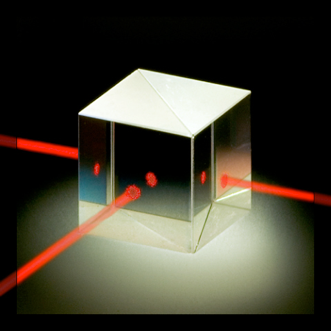
\includegraphics[scale=0.6]{./Bilder_QM/Polarizer2.png}
\end{picture}
\caption{\label{fig_Pol}%
\textbf{a} Ein Polw\"urfel oder Polarisationsstrahlteiler
besteht aus zwei zusammengesetzten Prismen
mit einer besonders pr\"aparierten 
Grenzfl\"ache. \textbf{b} Ein einfallender
(unpolarisierter) Strahl wird in zwei (orthogonal)
polarisierte Strahlen aufgespalten. Der reflektierte
Strahl besitzt eine Polarisation parallel zur 
Grenzfl\"ache ($v$) -- in der Abbildung senkrecht
zur Bildebene --, der durchgelassene Strahl
eine horizontale Polarisation ($h$) in der Bildebene. 
\textbf{c} Umgekehrt kann
man auch zwei geeignet polarisierte Strahlen zu einem
gemeinsamen Strahl zusammenf\"uhren. Die Polarisation
des ausfallenden Strahls h\"angt von der relativen Phase
der beiden einfallenden Strahlen ab. Bei Phasengleichheit
ist der ausfallende Strahl linear polarisiert, an\-sons\-ten
elliptisch. Bei umgekehrter Wahl der Polarisationen f\"ur die
einfallenden Strahlen verl\"auft der ausfallende Strahl
in der Abbildung nach oben. (rechts) Abbildung eines Polarizationsstrahlteilers. (aus \cite{Filk} und \cite{?})}
\end{figure}

In der Abbildung wurde der Polarisationsw\"urfel so aufgestellt, dass der durchgelassene
Strahl eine horizontale Polarisation besitzt, der (um $90^\circ$) reflektierte Strahl eine
vertikale Polarisation. Der Polarisationsw\"urfel kann aber auch um die Achse des einfallenden
Strahls gedreht werden, sodass eine Aufspaltung in zwei orthogonale Polarisationsrichtungen
bez\"uglich jeder Orientierung des W\"urfels vorgenommen werden kann. 

Eine \glqq Messung\grqq\ mit einem solchen Polarisationsw\"urfel kann dadurch erfolgen,
dass hinter den beiden Austrittsrichtungen f\"ur den Lichtstrahl ein Detektor platziert wird,
der das austretende Licht nachweist. Ohne die Detektoren kann man mit dieser Anordnung
eine Polarisation pr\"aparieren: Man verwendet einfach den Strahl, der an der Seite zu
der gew\"unschten Polarisation austritt, f\"ur die weiteren Versuche. 

Nun ist bekannt, dass ein Lichtstrahl aus einer sehr gro\ss en Anzahl von Photonen bzw.\
Lichtquanten besteht. Ein Laserpointer strahlt pro Sekunde rund $10^{18}-10^{20}$ Photonen ab.
Wenn man die Intensit\"at eines Laserstrahls immer weiter verringert, gelangt man schlie\ss lich
zu einzelnen Photonen. In der Praxis l\"asst sich das schwer realisieren, da es aufgrund der
bosonischen Eigenschaften von Photonen zu sogenannten Bunching-Effekten kommt: Photonen
treten bevorzugt als Mehrfachpakete auf. Man erh\"alt also keine Einzelphotonen mit
nahezu konstanten Zeitabst\"anden zwischen ihnen. Auf dieses eher technische Detail soll hier aber
nicht weiter eingegangen werden. Es ist im Prinzip (mit hohem Kostenaufwand) m\"oglich,
gezielt Einzelphotonen herzustellen und f\"ur die optischen Experimente, die hier eine Rolle spielen,
zu verwenden. 

F\"ur Einzelphotonen gelten im Wesentlichen dieselben Regeln, wie f\"ur einen Lichtstrahl. Lediglich
die Gesetze bez\"uglich der Intensit\"at von Lichtstrahlen werden durch Gesetze f\"ur relative H\"aufigkeiten
- und im Fall von Einzelphotonen durch Wahrscheinlichkeiten - ersetzt. So besagt das Gesetz
von Malus, dass die Intensit\"at eines Lichtstrahls, der einen Polarisationsfilter unter einer Orientierung
zum Winkel $\alpha$ durchquert hat und durch einen zweiten Filter tritt, der unter dem Winkel $\beta$ orientiert
ist, um den Faktor $\cos^2 (\alpha - \beta)$ verringert wird. F\"ur einen Strahl mit $N$ Photonen hinter dem
ersten Filter lautet dieses Gesetz: F\"ur die Anzahl $N_1$ der Photonen, die auch den zweiten Filter passieren, gilt
ungef\"ahr: $N_1/N = \cos^2(\alpha - \beta)$. Und f\"ur ein Einzelphoton lautet das Gesetz: Die Wahrscheinlichkeit,
dass ein Photon, welches den ersten Filter passiert hat, auch den zweiten Filter passiert, ist $\cos^2(\alpha - \beta)$. 

Zur Beschreibung der Polarisation von Einzelphotonen verwenden wir wieder normierte Vektoren
in einem zweidimensionalen komplexen Vektorraum. Die horizontale und vertikale Polarisation beschreiben
wir meist durch die Einheitsvektoren aus Gl.\ \ref{eq_QM1_Basis}, wobei wir in der Notation die klassischen
Bitvariablen durch $h$ und $v$ ersetzen:
\begin{equation}
           |h\rangle = \left(\!\! \begin{array}{c}  1 \\ 0 \end{array}\!\! \right)  \hspace{1cm}
           |v\rangle = \left(\!\! \begin{array}{c}  0 \\ 1 \end{array} \!\!\right)  \, . 
\end{equation} 
Unter den Winkeln $+45^\circ$ und $-45^\circ$ polarisiertes Licht dr\"ucken wir entsprechend durch
$+$ und $-$ aus. In der obigen Basis gilt f\"ur die Vektoren zu dieser Polarisation:
\begin{equation}
           |+\rangle = \frac{1}{\sqrt{2}} \left(\!\! \begin{array}{c}  1 \\ 1 \end{array}\!\! \right)  \hspace{1cm}
           |-\rangle = \frac{1}{\sqrt{2}} \left(\!\! \begin{array}{c}  1  \\ - 1 \end{array}\!\! \right)  \, . 
\end{equation} 
Linear polarisiertes Licht kann man dadurch beschreiben, dass die allgemeinen Koeffizienten
in Gl.\ \ref{eq_QM1_Einheitsvektor} reell gew\"ahlt werden k\"onnen. Dies bringt zum Ausdruck, dass es
keine relative Phasenverschiebung zwischen den beiden Komponenten (horizontal und vertikal) gibt. 
Eine Polarisation unter einem allgemeinen Winkel $\theta$ relativ zur Horizontalen wird durch den
Vektor
\begin{equation}
           |\theta \rangle =  \left( \!\!\begin{array}{c}  \cos \theta \\ \sin \theta \end{array} \!\!\right)    
\end{equation} 
beschrieben.

Neben den linearen Polarisationen gibt es noch die zirkularen Polarisationen (und ganz allgemein die
elliptischen Polarisationen):
\begin{equation}
           |L\rangle = \frac{1}{\sqrt{2}} \left(\!\! \begin{array}{c}  1 \\ {\rm i} \end{array} \!\!\right)  \hspace{1cm}
           |R\rangle = \frac{1}{\sqrt{2}} \left(\!\! \begin{array}{c}  1  \\ - {\rm i} \end{array}\!\! \right)  \, . 
\end{equation} 
Hier spricht man von links zirkular polarisiertem Licht bzw.\ rechts zirkular polarisiertem Licht. 
Ganz allgemein kann eine Polarisation durch den Vektor
\begin{equation}
\label{eq_QM1_allgPol}
     |\theta, \delta \rangle =  \left( \!\!\begin{array}{c}  \cos \theta  \\ {\rm e}^{{\rm i}\delta} \, \sin \theta  \end{array} \!\!\right)    
\end{equation} 
gekennzeichnet werden. Da eine beliebige gemeinsame Phase f\"ur die beiden Komponenten
denselben Zustand beschreibt, kann die erste Komponente reell gew\"ahlt werden. Der Winkel
$\delta$ gibt die Elliptizit\"at der Polarisation an ($\delta=0$ entspricht linear polarisiertem Licht
und $\delta=\pm 90^\circ$ entspricht R- bzw.\ L-zirkular polarisiertem Licht) und der Winkel $\theta$ kennzeichnet die
Lage der gro\ss en Halbachse dieser Ellipse.  

\subsection{Die Menge der Observablen}

In diesem Abschnitt betrachten wir die Menge der hermiteschen Matrizen in dem zweidimensionalen
komplexen Vektorraum, die wir mit der Menge der Observablen identifizieren werden. Als Basis f\"ur die hermiteschen
Matrizen bieten sich die drei Pauli-Matrizen sowie die Einheitsmatrix an:
\begin{equation}
   {\bf 1} = \left( \begin{array}{cc}  1 & 0 \\ 0 & 1 \end{array} \right)  \hspace{0.7cm}
   \sigma_1  = \left( \begin{array}{cc}  0 & 1 \\ 1 & 0 \end{array} \right)  \hspace{0.7cm}
   \sigma_2  = \left( \begin{array}{cc}  0 & -{\rm i} \\ {\rm i} & 0 \end{array} \right)  \hspace{0.7cm}
   \sigma_3 = \left( \begin{array}{cc}  0 & 1 \\ 0 & -1 \end{array} \right)  \, .
\end{equation}
Diese vier Matrizen sind hermitesch (d.h.\ es gilt $A_{ij}=A^*_{ji}$). Eine beliebige reelle Linearkombination
ist ebenfalls hermitesch. Umgekehrt l\"asst sich jede hermitesche $2\times 2$-Matrix als reelle Linearkombination
in dieser Form schreiben:
\begin{equation}
      A = a_0 {\bf 1} + \sum_{i=1}^3 a_i \sigma_i = a_0 {\bf 1} + \pmb{a} \cdot \pmb{\sigma}_i
         =     \left( \begin{array}{cc}  a_0 + a_3 & a_1+{\rm i}a_2 \\ a_1 - {\rm i}_2 &  a_0 - a_3 \end{array} \right) \, .
\end{equation} 
\"Uber das charakteristische Polynom erh\"alt man die Eigenwerte $\lambda_i$:
\begin{equation}
\label{eq_QM1_Eigenwerte}
           \lambda_{1/2} = a_0 \pm \sqrt{a_1^2 + a_2^2 + a_3^2} = a_0 \pm | \pmb{a} |  \, .
\end{equation} 
$\sigma_1$ hat als Eigenvektoren $|+\rangle$ und $|-\rangle$, $\sigma_2$ hat als Eigenvektoren
$|R\rangle$ und $|L\rangle$ und $\sigma_3$ hat die Eigenvektoren $|h\rangle$ und $|v\rangle$. Da es
sich bei $A$ um eine selbst-adjungierte Matrix handelt, sind die Eigenvektoren von $A$ immer orthogonal
zueinander. Es handelt sich bei den Eigenvektoren einer Observablen also immer um zueinander orthogonale 
Polarisationsvektoren.

\subsection{Die Bloch-Kugel}

Die Bloch-Kugel veranschaulicht die m\"oglichen Polarisationszust\"ande. Aus Gl.\ \ref{eq_QM1_allgPol} wird schon
deutlich, dass man die Polarisationszust\"ande durch zwei Winkel $\theta$ und $\delta$ charakterisieren kann,
wobei $\theta \in [0,\pi]$ (nach einer Drehung um $180^\circ$ erh\"alt man dieselbe lineare Polarisation) 
und $\delta \in [-\pi,+\pi]$ (positive Vorzeichen entsprechen rechtszirkularen elliptischen Polarisationen und
negative Vorzeichen linkszirkularen). Diese Darstellung legt schon nahe, dass es sich bei der Menge der
Polarisationszust\"ande um eine Kugeloberfl\"ache handelt. 
Trotzdem ist die Identifikation der Winkelvariablen nicht so trivial.

Wie schon erw\"ahnt, lassen sich die (reinen) Zust\"ande auch durch eindimensionale Projektionsmatrizen darstellen, 
also hermitesche Matrizen mit der Eigenschaft $P^2=P$. Diese Eigenschaft l\"asst nur die Eigenwerte 1 und 0 zu.
Ist ein Eigenwert 1 und der andere 0, projizieren diese
Matrizen auf eindimensionale Unterr\"aume. Aus Gl.\ \ref{eq_QM1_Eigenwerte} erkennt man, dass diese beiden
Eigenwerte nur in folgendem Fall auftreten:
\begin{equation}
      a_0 = \frac{1}{2}   \hspace{1cm} {\rm und} \hspace{1cm}  |\pmb{a}| = \frac{1}{2} \, .
\end{equation}
In zwei Dimensionen k\"onnen wir also jede Projektionsmatrix auf einen eindimensionalen Unterraum 
in der Form
\begin{equation}
         P =  \frac{1}{2} \Big( {\bf 1} + \pmb{n} \cdot \pmb{\sigma} \Big) 
\end{equation}
schreiben, wobei $\pmb{n}$ ein beliebiger 3-dimensionaler Einheitsvektor ist. Damit wird deutlich, dass sich jeder Zustand
durch einen 3-dimensionalen Einheitsvektor darstellen l\"asst. Diese Darstellung bezeichnet man als 
Bloch-Kugel (siehe Abb.\ \ref{fig_Bloch}).\footnote{Henri Poincar\'{e} hat schon 1892 diese Darstellung f\"ur die Polarisationszust\"ande
von Licht verwendet, daher wird sie in der Optik auch als Poincar\'{e}-Kugel bezeichnet.}

\begin{SCfigure}[50][htb]
\begin{picture}(200,180)(0,0)
\qbezier(20,90)(20,122)(43.4,146.6)
\qbezier(43.4,146.6)(68,170)(100,170)
\qbezier(20,90)(20,58)(43.4,33.4)
\qbezier(43.4,33.4)(68,10)(100,10)
\qbezier(180,90)(180,122)(156.6,146.6)
\qbezier(156.6,146.6)(132,170)(100,170)
\qbezier(180,90)(180,58)(156.6,33.4)
\qbezier(156.6,33.4)(132,10)(100,10)
%
\qbezier(20,90)(20,110)(100,110)
\qbezier(20,90)(20,70)(100,70)
\qbezier(100,110)(180,110)(180,90)
\qbezier(100,70)(180,70)(180,90)
%
\put(20,90){\line(1,0){160}}
\put(80,70.5){\line(1,1){39}}
\put(100,10){\line(0,1){160}}
%
\put(20,90){\makebox(0,0){$\bullet$}}
\put(100,10){\makebox(0,0){$\bullet$}}
\put(100,170){\makebox(0,0){$\bullet$}}
\put(180,90){\makebox(0,0){$\bullet$}}
\put(80,70.5){\makebox(0,0){$\bullet$}}
\put(120,109.5){\makebox(0,0){$\bullet$}}
\put(100,90){\makebox(0,0){$\bullet$}}
%
\put(10,90){\makebox(0,0){$|h \rangle$}}
\put(190,90){\makebox(0,0){$|v \rangle$}}
\put(100,2){\makebox(0,0){$|L \rangle$}}
\put(100,178){\makebox(0,0){$|R \rangle$}}
\put(80,62.5){\makebox(0,0){$| - \rangle$}}
\put(120,117.5){\makebox(0,0){$| + \rangle$}}
\put(114,83){\makebox(0,0){$\rho=\frac{1}{2}{\bf 1}$}}
\end{picture}
\caption{\label{fig_Bloch}%
Die Bloch-Kugel f\"ur Polarisationszust\"ande von Licht. Die Kugeloberfl\"ache
repr\"asentiert die reinen Zust\"ande, das Kugelinnere die gemischten
Zust\"ande. Gegen\"uberliegende Punkte (Antipoden) entsprechen orthogonalen Polarisationszust\"anden.}
\end{SCfigure}

F\"ur den Fall $|\pmb{n}|<1$ erh\"alt man sogenannte Dichtematrizen. Sie beschreiben gemischte
Zust\"ande aus verschiedenen Polarisationen. Der Spezialfall $|\pmb{n}|=0$ f\"uhrt auf die Einheitsmatrix
(multipliziert mit $1/2$). In diesem Fall kann keine Aussage \"uber die Polarisation getroffen werden bzw.\
alle Polarisationsrichtungen sind gleich wahrscheinlich. Dies ist der maximal gemischte Zustand. Das 
Innere der Bloch-Kugel kennzeichnet somit gemischte Zust\"ande, die Oberfl\"ache die reinen Zust\"ande. 

Man beachte, dass die Bloch-Kugel in einem 3-dimensionalen reellen Vektorraum liegt. Orthogonale
Polarisationen ($h$ und $v$ oder $+$ und $-$ oder auch $L$ und $R$) liegen auf der Bloch-Kugel antipodisch
gegen\"uber. Es handelt sich bei diesem Vektorraum daher nicht um den Hilbert-Raum der Zust\"ande, in dem
orthogonale Polarisationen auch durch orthogonale Vektoren dargestellt werden.

\section{Verschr\"ankung}

Ebenso wie in der klassischen Informationstheorie interessiert man sich in der Quanteninformation
nicht nur f\"ur einzelne QuBits, sondern f\"ur Ketten bzw.\ Folgen von QuBits. Im Folgenden betrachten wir
nur QuBit-Paare, also Systeme zur Darstellung von zwei QuBits. Es zeigt sich, dass man auch in der
Quantentheorie (\"ahnlich wie in der klassischen Informationstheorie) die meisten Operationen auf
QuBit-Folgen als Hintereinanderausf\"uhrung von Operationen auf QuBit-Paaren darstellen kann. 

Ein System aus zwei QuBits (z.B.\ die Polarisationszust\"ande von zwei Photonen) wird im Tensorprodukt
der beiden einzelnen zweidimensionalen Vektorr\"aume beschrieben. Man erh\"alt auf diese Weise einen
vierdimensionalen komplexen Vektorraum. In einem solchen Tensorprodukt
beschreibt man die Vektoren gerne mit Doppelindizes. So ist bespielsweise das Tensorprodukt aus
einem Vektor $\pmb{x}$ und einem Vektor $\pmb{y}$ gegeben durch:
\begin{equation}
\label{eq_QM1_Tensor}
       \pmb{x} \otimes \pmb{y} = \left( \begin{array}{c} x_1 \\ x_2 \end{array} \right) \otimes
          \left( \begin{array}{c} y_1 \\ y_2 \end{array} \right) =
           \left( \begin{array}{c} x_1 y_1  \\ x_1 y_2 \\ x_2 y_1 \\ x_2 y_2  \end{array} \right)
%           \simeq  \left( \begin{array}{cc} x_1 y_1 &  x_1 y_2 \\ x_2 y_1 & x_2 y_2  \end{array} \right)  
            \, .
\end{equation}
Das Tensorprodukt der beiden Vektorr\"aume besteht aus allen Linearkombinationen solcher
Vektoren, wobei folgendes Distributivgesetz gilt:\footnote{Man beachte den Unterschied zur
direkten Summe von Vektorr\"aumen bzw.\ Vektoren:
\[      (\pmb{x}_1 + \pmb{x}_2) \oplus (\pmb{y}_1 + \pmb{y}_2) = \pmb{x}_1  \oplus \pmb{y}_1 +
     \pmb{x}_2  \oplus \pmb{y}_2  \, . \]  
und $\pmb{0} \oplus \pmb{y}$ sowie $\pmb{x}\oplus \pmb{0}$ sind von null verschiedene Vektoren. Statt
$\pmb{x} \oplus \pmb{y}$ schreibt man hier oft einfacher $(\pmb{x},\pmb{y})$.}
\begin{equation}
     (\pmb{x}_1 + \pmb{x}_2) \otimes (\pmb{y}_1 + \pmb{y}_2) = \pmb{x}_1  \otimes \pmb{y}_1 +
     \pmb{x}_1  \otimes \pmb{y}_2 +\pmb{x}_2  \otimes \pmb{y}_1 +\pmb{x}_2  \otimes \pmb{y}_2 
\end{equation}
sowie
\begin{equation}
     \pmb{0} \otimes \pmb{y} = \pmb{x} \otimes \pmb{0} = \pmb{0} \, .
\end{equation}

Man erkennt sofort, dass in Gl.\ \ref{eq_QM1_Tensor} das Produkt der beiden \"au\ss eren Komponenten 
(die erste und vierte Komponente) gleich dem 
Produkt der beiden inneren Komponenten ist. Dies kennzeichnet den Vektor (in zwei Dimensionen) eindeutig
als separabel, wobei ein Vektor in dem vierdimensionalen Vektorraum als separabel bezeichnet wird, wenn
es zwei Vektoren $\pmb{x}$ und $\pmb{y}$ in den einzelnen Vektorr\"aumen gibt, sodass sich der
vierdimensionale Vektor als Tensorprodukt der beiden zweidimensionalen Vektoren schreiben l\"asst. 
Falls das nicht m\"oglich ist - allgemein sich also ein Vektor in einem Tensorproduktraum nicht als Tensorprodukt
von zwei Vektoren in den einzelnen Vektorr\"aumen schreiben l\"asst - bezeichnet man den Vektor
als verschr\"ankt. In zwei Dimensionen haben wir somit ein einfaches Kriterium f\"ur die Verschr\"anktheit
von zwei Vektoren: Wenn das Produkt der ersten und vierten Komponente eines Vektors nicht gleich dem
Produkt der zweiten und dritten Komponente ist, ist der Vektor verschr\"ankt. 

Bei Wellenfunktionen zu zwei Teilsystemen (oder allgemeiner zu zwei unabh\"angigen Klassen von
Freiheitsgraden), die durch Funktionen von zwei Variablen beschrieben werden, bedeutet Separierbarkeit,
dass $\Psi(x,y)= \varphi(x) \psi(y)$. Die Wellenfunktion l\"asst sich also als einfaches Produkt von zwei
Funktionen darstellen. F\"ur verschr\"ankte Wellenfunktionen gilt das nicht. 

Man beachte, dass der Begriff der Verschr\"anktheit nur sinnvoll ist, wenn f\"ur einen Vektorraum eine
Zerlegung als ein Tensorprodukt definiert ist. Ohne die Angabe einer solchen Produktdarstellung ist
der Begriff der Verschr\"ankung nicht definiert. Die Angabe einer solchen Produktdarstellung gibt an,
in welcher Form das Gesamtsystem als aus zwei Teilsystemen bestehend gedacht werden kann. Bei
zwei Teilchen ist eine solche Zerlegung physikalisch naheliegend (jedes Teilchen definiert sein Teilsystem). 
Es kann jedoch auch eine Verschr\"ankung beispielsweise zwischen den Polarisationsfreiheitsgraden
eines Photons und seinen r\"aumlichen Eigenschaften bestehen. So hat ein einzelnes Photon, das
durch einen Doppelspalt tritt, wobei hinter dem rechten Spalt ein $+$-Polarisationsfilter und hinter dem
linken Spalt ein $-$-Polarisationsfilter steht, eine Verschr\"ankung zwischen seiner Polarisation und dem
Spalt, durch den es getreten ist. Der Zustand
\begin{equation}
        | \gamma \rangle = \frac{1}{\sqrt{2}} \Big( |+\rangle \otimes |r \rangle + |- \rangle \otimes |l\rangle \Big)
\end{equation}
beschreibt ein solches Photon. Die $+$-Polarisation ist korreliert mit dem rechten Spalt und die $-$-Polarisation
mit dem linken. Dieser Zustand ist im Sinne der obigen Definition verschr\"ankt. Die Darstellung des Zustands
einzelner Photonen durch solche Verschr\"ankungen
zwischen ihrem Polarisationsfreiheitsgrad und ihrer r\"aumlichen Eigenschaft ist
ganz sinnvoll, beispielsweise bei der Beschreibung von Experimenten zum Quantenradierer. Meistens hat man es aber mit
Verschr\"ankungen zwischen den Polarisationszust\"anden (bzw.\ allgemeiner den zwei Zust\"anden) 
eines Systems aus zwei Teilchen zu tun. 

Die physikalische Bedeutung der Verschr\"ankung liegt unter anderem an folgender Eigenschaft 
verschr\"ankter Zust\"ande. Ist ein Zustand separierbar, so separiert auch das Absolutquadrat 
der Komponenten des Vektors, durch den der Zustand beschrieben wird (vgl.\ Gl.\ \ref{eq_QM1_Tensor}).
Diese Absolutquadrate entsprechen aber nach der Born'schen Regel 
bei Einzelsystemen den Wahrscheinlichkeiten, dass 
zwei Ereignisse gleichzeitig auftreten (bei Funktionenr\"aumen handelt es sich um Wahrscheinlichkeitsdichten,
die zur Berechnung einer Wahrscheinlichkeit \"uber ein Volumen zu integrieren sind). Beispielsweise ist
in Gl.\ \ref{eq_QM1_Tensor} $w_{ij}=|x_i|^2|y_j|^2$ die Wahrscheinlichkeit f\"ur das gleichzeitige Auftreten der
beiden Ereignisse $i$ und $j$. Faktorisierende
Wahrscheinlichkeiten f\"ur zwei Ereignisse bedeutet aber, dass diese Ereignisse unkorreliert sind. 
Eine Information \"uber das Vorliegen eines der beiden Ereignisse \"andert nichts an der Wahrscheinlichkeit
f\"ur das Auftreten des zweiten Ereignisses. 

Bei verschr\"ankten Zust\"anden ist dies anders: Erh\"alt man eine Information \"uber das Vorliegen eines
Ereignisses beispielsweise an einem Teilsystem, kann man neue Vorhersagen \"uber das Eintreffen eines 
anderen Ereignisses an dem anderen Teilsystem treffen. Im Extremfall liegt das Ereignis an dem anderen
Teilsystem sogar eindeutig fest. Dies ist dann besonders erstaunlich, wenn die beiden Teilsysteme
sehr weit voneinander entfernt sind. Weshalb sollte eine Messung an einem Teilsystem auf der Erde
eine instantane Ver\"anderung des anderen Teilsystems im Andromeda-Nebel zur Folge haben? Diese
Eigenschaft verschr\"ankter Zust\"ande h\"angt eng mit der Problematik der Lokalit\"at der Quantentheorie
zusammen. 

\section{Bell-Zust\"ande}

In dem Tensorproduktraum von zwei Zwei-Zustandssystemen gibt es eine ausgezeichnete Basis, die man erh\"alt,
wenn man die Tensorprodukte der Basisvektoren in den einzelnen Hilbert-R\"aumen bildet:
\begin{equation}
           |h\rangle \otimes |h\rangle = \left( \begin{array}{c}  1 \\ 0 \\ 0 \\ 0 \end{array} \right) \hspace{0.4cm}
           |h\rangle \otimes |v\rangle = \left( \begin{array}{c}  0 \\ 1 \\ 0 \\ 0 \end{array} \right) \hspace{0.4cm}
           |v\rangle \otimes |h\rangle = \left( \begin{array}{c}  0 \\ 0 \\ 1 \\ 0 \end{array} \right) \hspace{0.4cm}
           |v\rangle \otimes |v\rangle = \left( \begin{array}{c}  0 \\ 0 \\ 0 \\ 1 \end{array} \right) \, .
\end{equation}
Diese Basisvektoren sind alle separabel. Zur Beschreibung von verschr\"ankten Zust\"anden bietet es sich
oft an, eine Basis zu w\"ahlen, bei der alle Basisvektoren maximal verschr\"ankt sind.\footnote{Es gibt eine
technische Definition von maximal verschr\"ankt: Wenn die Spur \"uber die Projektionsmatrix des Zustands 
\"uber einen der Teilr\"aume die Identit\"atsmatrix in dem verbliebenen Teilraum ergibt. Physikalischer
ausgedr\"uckt: Ein Zustand hei\ss t maximal verschr\"ankt, wenn der Erwartungswert f\"ur beliebieg 
Messungen an einem Teilsystem durch eine Dichtematrix proportional zur Identit\"atsmatrix - also maximale
Unkenntnis - beschrieben werden muss. Dies wird im Folgenden
aber nicht ben\"otigt.} Die Orthonormalbasis aus den folgenden vier Zust\"anden hat diese Eigenschaft.
Diese Zust\"ande bezeichnet man als Bell-Zust\"ande:
\begin{eqnarray}
      |\Phi^+ \rangle &=&  \frac{1}{\sqrt{2}} \Big( |h\rangle \otimes |h\rangle + |v\rangle \otimes |v\rangle \Big)
            = \frac{1}{\sqrt{2}} \left( \begin{array}{c}  1 \\ 0 \\ 0 \\ 1 \end{array} \right)   \\[0.2cm]  
      |\Phi^- \rangle &=&  \frac{1}{\sqrt{2}} \Big( |h\rangle \otimes |h\rangle - |v\rangle \otimes |v\rangle \Big)
            = \frac{1}{\sqrt{2}} \left( \begin{array}{c}  1 \\ 0 \\ 0 \\ -1 \end{array} \right)   \\[0.2cm]
      |\Psi^+ \rangle &=&  \frac{1}{\sqrt{2}} \Big( |h\rangle \otimes |v\rangle + |v\rangle \otimes |h\rangle \Big)
            = \frac{1}{\sqrt{2}} \left( \begin{array}{c}  0 \\ 1 \\ 1 \\ 0 \end{array} \right)   \\[0.2cm]  
      |\Psi^- \rangle &=&  \frac{1}{\sqrt{2}} \Big( |h\rangle \otimes |v\rangle - |v\rangle \otimes |h\rangle \Big)
            = \frac{1}{\sqrt{2}} \left( \begin{array}{c}  0 \\ 1 \\ - 1 \\ 0 \end{array} \right)    \, .
\end{eqnarray}
Den letzten Zustand, $|\Psi^- \rangle$, bezeichnet man auch oft als EPR-Zustand (nach Einstein-Podolsky-Rosen). 
Er hat einige besondere Eigenschaften, insbesondere liegt die Antikorrelation bez\"uglich jeder Basis vor, d.h.\
es gilt:
\begin{equation}
  |{\rm EPR} \rangle = \frac{1}{\sqrt{2}} \Big( |h\rangle \otimes |v\rangle - |v\rangle \otimes |h\rangle \Big) 
  = \frac{1}{\sqrt{2}} \Big( |+\rangle \otimes |-\rangle - |-\rangle \otimes |+\rangle \Big) =
    \frac{1}{\sqrt{2}} \Big( |R\rangle \otimes |L\rangle - |L\rangle \otimes |R\rangle \Big) \, .
\end{equation}
Es handelt sich bei diesem Bell-Zustand um den Eigenzustand zum Gesamtdrehimpuls 0 (Photonen haben einen
Spin 1, und zwei Photonen k\"onnen sich zum Gesamtspin 0 oder Gesamtspin 2 verbinden). Dieser Zustand
ist invariant unter Drehungen und daher in allen Basissystemen formgleich. F\"ur den Zustand $|\Phi^+\rangle$
gilt diese Eigenschaft, sofern man sich auf lineare Polarisationen beschr\"ankt.
 


\begin{thebibliography}{99}
\bibitem{Aspect} Aspect, A., Grangier, Ph., Roger, G.; 
       {Experimental Realization of Einstein-Podolsky-Rosen-Bohm 
        Gedankenexperiment: A New Violation of Bell's Inequalities}; 
        Phys.\ Rev.\ Lett.\ 49 (1982) 91--94. \\
        Aspect, A., Dalibard, J., Roger, G.; {Experimental Test 
        of Bell's Inequalities Using Time-Varying Analyzers}; 
        Phys.\ Rev.\ Lett.\ 49 (1982) 1804--1807.
\bibitem{Bell} Bell, J.; {\em Against \glq Measurement\grq};
        in {\em 62 Years of Uncertainty}, Erice, 5--14 August 1989;
        auch in {\em Physics World} 8 (1990) 33--40. Abgedruckt in
        \cite{Bell2}. 
\bibitem{Bell2} Bell, J.S.;  {\em Speakable and Unspeakable in 
        Quantum Physics}, 2.\ edition, Cambridge University Press (2004).         
        \bibitem{Filk} Filk, T; \textit{Quantenmechanik (nicht nur) f\"ur Lehramtsstudierende}; Springer-Verlag, 2019.
\bibitem{Schroedinger} Schr\"odinger, E.; {\em Die gegenw\"artige
        Situation in der Quantenmechanik}; Die Naturwissenschaften 23
        (1935) 807--812, 823--828,  844-849.      
\end{thebibliography}

%\end{document}


%\documentclass[german,10pt]{book}      
\usepackage{makeidx}
\usepackage{babel}            % Sprachunterstuetzung
\usepackage{amsmath}          % AMS "Grundpaket"
\usepackage{amssymb,amsfonts,amsthm,amscd} 
\usepackage{mathrsfs}
\usepackage{rotating}
\usepackage{sidecap}
\usepackage{graphicx}
\usepackage{color}
\usepackage{fancybox}
\usepackage{tikz}
\usetikzlibrary{arrows,snakes,backgrounds}
\usepackage{hyperref}
\hypersetup{colorlinks=true,
                    linkcolor=blue,
                    filecolor=magenta,
                    urlcolor=cyan,
                    pdftitle={Overleaf Example},
                    pdfpagemode=FullScreen,}
%\newcommand{\hyperref}[1]{\ref{#1}}
%
\definecolor{Gray}{gray}{0.80}
\DeclareMathSymbol{,}{\mathord}{letters}{"3B}
%
\newcounter{num}
\renewcommand{\thenum}{\arabic{num}}
\newenvironment{anmerkungen}
   {\begin{list}{(\thenum)}{%
   \usecounter{num}%
   \leftmargin0pt
   \itemindent5pt
   \topsep0pt
   \labelwidth0pt}%
   }{\end{list}}
%
\renewcommand{\arraystretch}{1.15}                % in Formeln und Tabellen   
\renewcommand{\baselinestretch}{1.15}                 % 1.15 facher
                                                      % Zeilenabst.
\newcommand{\Anmerkung}[1]{{\begin{footnotesize}#1 \end{footnotesize}}\\[0.2cm]}
\newcommand{\comment}[1]{}
\setlength{\parindent}{0em}           % Nicht einruecken am Anfang der Zeile 

\setlength{\textwidth}{15.4cm}
\setlength{\textheight}{23.0cm}
\setlength{\oddsidemargin}{1.0mm} 
\setlength{\evensidemargin}{-6.5mm}
\setlength{\topmargin}{-10mm} 
\setlength{\headheight}{0mm}
\newcommand{\identity}{{\bf 1}}
%
\newcommand{\vs}{\vspace{0.3cm}}
\newcommand{\noi}{\noindent}
\newcommand{\leer}{}

\newcommand{\engl}[1]{[\textit{#1}]}
\parindent 1.2cm
\sloppy

         \begin{document} 
\setcounter{page}{1}
\setcounter{section}{0}
\setcounter{figure}{0}
\setcounter{equation}{0}
\setcounter{table}{0}
\setcounter{footnote}{0}

\section*{Interferometer}

\noindent
{\bf Thomas Filk; Universit\"at Freiburg}
\vspace{1cm}
% Kap x
\label{chap_Interferometer}

\noindent
Interferometer spielen \"uberall in der Optik eine wichtige Rolle. Sie sind eines
der zentralen Instrumente der Experimentalphysik f\"ur optische und quantenoptische Versuche. Verwendet man
Laserlicht, zeigen Interferometer unter anderem die Wellennatur des Lichts. Mit Einzelphotonen
lassen sich jedoch vollkommen neuartige und interessante Effekte erzielen. 

Zwei der bekanntesten Interferometer sind das Mach-Zehnder-Interferometer und
das Michelson-Interferometer. Beide beruhen auf einem \"ahnlichen Prinzip: Ein Strahl
wird mit einem Strahlteiler geteilt, \"uber ein Spiegelsystem auf einen zweiten Strahlteiler gelenkt
und dort wieder zusammengebracht, wobei dann die Interferenzmuster entstehen. Beim Michelson-Interferometer
gibt es nur einen Strahlteiler, der sowohl die Aufspaltung als auch die sp\"atere
Zusammenf\"uhrung \"ubernimmt, d.h.\ das Spiegelsystem reflektiert die aufgeteilten 
Strahlen wieder zur\"uck auf den ersten Strahlteiler, hinter dem es dann zur Interferenz kommen kann. Beim 
Mach-Zehnder-Interferometer lenken die Spiegel die beiden Strahlen auf einen
zweiten Strahlteiler, hinter dem dann eventuell Interferenzen beobachtet werden k\"onnen.  


Beide Interferometer lassen sich sowohl mit gew\"ohnlichen Strahlteilern als auch
mit polarisationsabh\"angigen Strahlteilern betreiben. Allerdings ist dies beim Michelson-Interferometer
etwas problematischer, da dort die vorgegebene Orientierung die Strahlen in die Lichtquelle
lenken w\"urde, wohingegen man einen Ausgang m\"ochte, der senkrecht dazu steht. 
Das Michelson-Interferometer wird auch beim Nachweis von Gravitationswellen verwendet. 

Viele Experimente lassen sich am Mach-Zehnder-Interferometer leichter beschreiben,
aber am Michelson-Interferometer leichter durchf\"uhren. Daher sollen hier beide Interferometer
besprochen werden. In gewissen Hinsicht sind diese Interferometer Erweiterungen des
Doppelspaltexperiments f\"ur koh\"arentes Licht: Der Strahl bzw.\ der Zustand eines einzelnen Photons
wird aufgeteilt und die beiden Anteile breiten sich entlang unterschiedlicher Wege aus bevor
sie wieder zusammengef\"uhrt und zur Interferenz gebracht werden. Allerdings kann man an
diesen Interferometern die beiden Teile eines Strahls bzw.\ eines Photonzustands im Prinzip beliebig weit
auseinander bringen, was den Effekt erh\"oht. Au\ss erdem kann man optische
Ger\"ate oder Hinternisse in den Weg einer der Teilstrahlen bringen. In der Schule werden viele
der (Gedanken-)Experimente mit Mach-Zender- bzw.\ Michelson-Interferometern unter dem
Gesichtspunkt \glqq Ist Welcher-Weg-Information bekannt?\grqq\ behandelt, d.h.\ die Aufgabe
der Sch\"uler*innen besteht darin zu entscheiden, ob man je nach experimentellem Aufbau
im Prinzip die Information dar\"uber, welchen Weg ein Photon genommen hat, gewinnen kann
oder nicht. In Abh\"angigkeit davon kann man dann entscheiden, ob ein Interferenzmuster beobachtet werden
kann oder nicht.  

Beide Interferometer werden f\"ur den Fall normaler (d.h., nicht polarisationsabh\"angiger) 
Strahlteilern beschrieben. Ein anderer Abschnitt widmet sich dem Mach-Zehnder-Interferometer 
mit polarisationsabh\"angigen Strahlteilern. Wir beginnen allerdings mit einer
kurzen Beschreibung der mathematischen Darstellung eines Strahlteilers.

\section{Strahlteiler}

Strahlteiler sind die wesentlichen Elemente eines Mach-Zehnder- bzw.\ Michelson-Interferometers.
Es gibt polarisationsabh\"angige Strahlteiler, bei denen ein einfallender Lichtstrahl in zwei
Teilstrahlen mit zueinander orthogonalen Polarisationszust\"anden aufgespalten wird. H\"aufiger
verwendet man jedoch nicht polarisationsabh\"angige Strahlteiler, d.h., der einfallende Strahl wird koh\"arent
in zwei gleichartig polarisierte Teilstrahlen aufgeteilt. 

Physikalisch besteht ein Strahlteiler meist aus einer beschichteten Grenzfl\"ache. Die Beschichtung ist
gerade so gew\"ahlt, dass die H\"alfte der Lichtintensit\"at durchgelassen und die andere H\"alfte
abgelenkt wird. Es gibt auch Strahlteiler mit einer asymmetrischen Aufspaltung, wir beschr\"anken uns
hier aber auf die Halbe-Halbe-Strahlteiler.

Wir k\"onnen die Wirkung eines Strahlteilers 
durch eine unit\"are Matrix beschreiben (unit\"ar, weil zumindest in der Theorie keine Intensit\"at 
verloren geht, d.h.,\ alle Photonen, die in den Strahlteiler eindringen, kommen auch wieder heraus). 
Diese Matrix ergibt sich auch direkt aus der \"Uberlegung, wie zwei einfallende Strahlen am
Strahlteiler aufgeteilt werden. Diese beiden Vorschriften sind:
\begin{equation}
\label{eq_ST1}
       |  1 \rangle_{\rm i}  \longrightarrow  \frac{1}{\sqrt{2}} \big( |1 \rangle_{\rm f} + {\rm i} | 2 \rangle_{\rm f} \big)
       \hspace{2cm}
    |  2 \rangle_{\rm i}  \longrightarrow  \frac{1}{\sqrt{2}} \big( | 2 \rangle_{\rm f} + {\rm i} | 1 \rangle_{\rm f} \big)       
\end{equation}
Hierbei wurde die in der Streutheorie \"ubliche Konvention verwendet, die einlaufenden (`initial')
Zust\"ande durch i und die auslaufenden (`final') Zust\"ande durch f zu kennzeichnen. Die
(Streu-)Matrix zum Strahlteiler ist dann durch $S_{ij}={}_{\rm f}\langle j | i \rangle_{\rm i}$ gegeben, also
durch die Wahrscheinlichkeitsamplituden zu dem \"Ubergang von einem Anfangzustand $i$  
zu einem Ausgangszustand $j$ (siehe auch Abb.\ \ref{fig_ST}). Die Faktoren i in Gl.\ \ref{eq_ST1}
beschreiben eine relative Phasenverschiebung um $90^\circ$. Diese Phasenverschiebung tritt immer
auf, wenn eine Reflektion an einer einer Grenzschicht stattfindet, bei der der Winkel zwischen
einfallender und ausfallender Welle gerade $90^\circ$ betr\"agt. Der Faktor $1/\sqrt{2}$ ergibt sich 
daraus, dass das Quadrat dieses Faktors nach der Born'schen
Regel die Wahrscheinlichkeit angibt, das Photon in dem jeweiligen Sektor zu messen (hier
jeweils $1/2$). F\"ur
Laserlicht bedeutet er einfach, dass jeder Teilstrahl die H\"alfte der Eingangsintensit\"at besitzt. 

\begin{SCfigure}[30][htb]
\begin{picture}(100,100)(-5,0)
\put(10,50){\line(1,0){80}}
\put(50,50){\line(0,1){40}}
\put(30,50){\vector(1,0){0}}
\put(80,50){\vector(1,0){0}}
\put(50,80){\vector(0,1){0}}
\put(90,58){\makebox(0,0){$|1\rangle_{\rm f}$}}
\put(42,90){\makebox(0,0){$|2\rangle_{\rm f}$}}
\put(10,58){\makebox(0,0){$|1\rangle_{\rm i}$}}
\thicklines
\put(29,29){\line(1,1){40}}
\put(31,31){\line(1,1){40}}
\end{picture}
%
\begin{picture}(110,100)(0,0)
\put(50,50){\line(1,0){40}}
\put(50,10){\line(0,1){80}}
\put(50,30){\vector(0,1){0}}
\put(80,50){\vector(1,0){0}}
\put(50,80){\vector(0,1){0}}
\put(90,58){\makebox(0,0){$|1\rangle_{\rm f}$}}
\put(42,90){\makebox(0,0){$|2\rangle_{\rm f}$}}
\put(58,15){\makebox(0,0){$|2\rangle_{\rm i}$}}
\thicklines
\put(29,29){\line(1,1){40}}
\put(31,31){\line(1,1){40}}
\end{picture}
\caption{\label{fig_ST}%
Die beiden Strahleng\"ange in einem Strahlteiler in Abh\"angigkeit vom
Anfangszustand. Ordnet man jeder Reflektion
einen Faktor i zu, erh\"alt man die Matrix in Gl.\ \ref{eq_STrep1}.}
\end{SCfigure}


Damit erhalten wir die folgende unit\"are Matrix, die das Verhalten von Photonen bzw.\
Licht an einem Halbe-Halbe-Strahlteiler beschreibt:
\begin{equation}
\label{eq_STrep1}
                 S = \frac{1}{\sqrt{2}}  \left( \begin{array}{cc}  1 & {\rm i} \\ {\rm i} & 1 \end{array} \right)  \, .
\end{equation}

Man kann noch relative optische Wegl\"angen\"anderungen (Phasen) vor- bzw.\ nachschalten.
Diese werden durch eine Diagonalmatrix mit reinen Phasen beschrieben. Auf diese Weise erhalten
wir eine allgemeine Darstellung f\"ur $S$ in der Form:
\begin{equation}
        S(\alpha,\beta) = \frac{1}{\sqrt{2}} 
        \left( \begin{array}{cc}  {\rm e}^{{\rm i}\alpha} & 0 \\ 0 & {\rm e}^{-{\rm i}\alpha} \end{array} \right)
          \left( \begin{array}{cc}  1 & {\rm i} \\ {\rm i} & 1 \end{array} \right)
          \left( \begin{array}{cc}  {\rm e}^{{\rm i}\beta} & 0 \\ 0 & {\rm e}^{-{\rm i}\beta} \end{array} \right)
  =  \frac{1}{\sqrt{2}}   
    \left( \begin{array}{cc}  {\rm e}^{{\rm i}(\alpha+\beta)} & {\rm i} {\rm e}^{{\rm i}(\beta-\alpha)} \\ 
                   {\rm i} {\rm e}^{{\rm i}(\alpha-\beta)} & {\rm e}^{-{\rm i}(\alpha+\beta)} \end{array} \right)
\end{equation}
Durch die spezielle Wahl $\alpha = - \beta = \pi/4$ erhalten wir eine andere Darstellung f\"ur
einen Strahlteiler, die ebenfalls h\"aufig verwendet wird:
\begin{equation}
\label{eq_STrep2}
                 S' = \frac{1}{\sqrt{2}}  \left( \begin{array}{cc}  1 & 1 \\ -1 & 1 \end{array} \right)  \, .
\end{equation}
Das Minuszeichen in der Matrix ist 
wesentlich, da es sich andernfalls nicht um eine unit\"are Matrix handeln w\"urde. Dieses Minuszeichen
beschreibt letztendlich die relative Phasenverschiebung von $180^\circ$ zwischen den beiden
reflektierten Strahlen. Anders ausgedr\"uckt: Die Summe der relativen Phasen der reflektierten Strahlen 
ist $180^\circ$, die Summe der relativen Phasen der durchgelassenen Strahlen ist $0^\circ$. 
Dieses Minuszeichen ist aber gerade Sch\"uler*innen kaum einfach zu vermitteln,
wohingegen die obige Erkl\"arung einsichtiger ist und auf dasselbe Ergebnis f\"uhrt. 

\section{Das Mach-Zehnder-Interferometer}

Beim Mach-Zehnder-Interferometer trifft ein Lichtstrahl zun\"achst auf einen Strahlteiler.
Ein Teil des Lichtstrahls wird abgelenkt, der andere Teil durchgelassen. \"Uber zwei Spiegel,
an denen die Lichtstrahlen um jeweils $90^\circ$ reflektiert werden, treffen beide
Strahlen von verschiedenen Seiten auf einen zweiten Strahlteiler, wo sie wieder
zusammengef\"uhrt werden. Hinter dem zweiten Strahlteiler kann man die Intensit\"at
des Lichts an zwei m\"oglichen Ausg\"angen messen. 

\begin{SCfigure}[30][htb] 
%\unitlength 2pt
\begin{picture}(300,170)(-5,0)
\thicklines
\put(40,10){\line(1,1){20}}
\put(250,10){\line(1,1){20}}
\put(251,9){\line(1,1){20}}
\put(40,120){\line(1,1){20}}
\put(39,121){\line(1,1){20}}
\put(250,120){\line(1,1){20}}
\thinlines
\put(0,20){\line(1,0){260}}
%\put(60,20){\circle*{10}}
\put(50,20){\line(0,1){110}}
\put(260,20){\line(0,1){110}}
\put(50,130){\line(1,0){210}}
\put(20,20){\vector(1,0){0}}
\put(150,20){\vector(1,0){0}}
\put(150,130){\vector(1,0){0}}
\put(50,70){\vector(0,1){0}}
\put(260,70){\vector(0,1){0}}
\put(260,130){\vector(1,0){20}}
\put(260,130){\vector(0,1){20}}
%
\put(25,30){\makebox(0,0){$|\gamma \rangle$}}
\put(150,30){\makebox(0,0){$| {\rm t} \rangle$}}
\put(60,70){\makebox(0,0){$|{\rm r} \rangle$}}
\put(250,150){\makebox(0,0){$| {\rm D} \rangle$}}
\put(275,120){\makebox(0,0){$|{\rm C} \rangle$}}
%
%\put(260,170){\makebox(0,0){\footnotesize D dunkel}}
%\put(300,130){\makebox(0,0){\footnotesize C hell}}
\put(70,10){\makebox(0,0){\footnotesize Strahlteiler}}
\put(220,120){\makebox(0,0){\footnotesize Strahlteiler}}
\put(70,146){\makebox(0,0){\footnotesize Spiegel}}
\put(280,37){\makebox(0,0){\footnotesize Spiegel}}
%
\end{picture} 
\caption{\label{fig_MachZehnder}%
Mach-Zehnder-Interferometer. Der Strahl trifft auf einen ersten Strahlteiler. Die beiden
Teil\-strahlen r und t werden von Spiegeln auf einen zweiten Strahlteiler gelenkt, hinter dem
es zu konstruktiver bzw.\ destruktiver Interferenz kommen kann.} 
\end{SCfigure}

Die Interferenz am Ausgang hinter dem zweiten Strahlteiler ergibt sich aus unterschiedlichen
optischen Wegl\"angen der zwei Strahlen, die dort zusammentreffen. Meist findet man
folgende, sehr vereinfachte Erkl\"arung: Am Ausgang $D$ treffen zwei Strahlen aufeinander,
von denen einer einmal um $90^\circ$ reflektiert wurde und der andere dreimal. Da jede
Reflektion um $90^\circ$ eine Phasenverschiebung von $90^\circ$ zur Folge hat 
ergibt sich zwischen den beiden Strahlen eine relative Phasenverschiebung
von $180^\circ$ und somit destruktive Interferenz. Bei Ausgang $C$ treffen zwei Strahlen
aufeinander, die jeweils einmal reflektiert wurden und somit in Phase sind; es kommt also zu
konstruktiver Interferenz. 

Im mathematischen Formalismus f\"ur Einzelphotonen k\"onnen wir dies folgenderma\ss en
beschreiben. Ein einfallendes Photon wird durch den Vektor $|\gamma\rangle$ beschrieben.
Am ersten Strahlteiler (ST) wird dieser Zustand in eine Superposition von zwei Zust\"anden 
zerlegt: einer dieser Zust\"ande ist der Zustand $|{\rm t}\rangle$ (f\"ur transmittiert), der andere ist der
Zustand des reflektierten Anteils $|{\rm r}\rangle$. Der reflektierte Anteil erh\"alt noch eine Phase von
$90^\circ$, was durch einen Faktor i ausgedr\"uckt werden kann. Hinter dem ersten Strahlteiler
erhalten wir also folgenden Zustand:
\begin{equation}
           |\gamma \rangle  \longrightarrow  \frac{1}{\sqrt{2}} \big( |{\rm t}\rangle + {\rm i} |{\rm r}\rangle \big) \, .
\end{equation}
Der Faktor $1/\sqrt{2}$ ergibt sich daraus, dass das Quadrat dieses Faktors nach der Born'schen
Regel die Wahrscheinlichkeit angibt, das Photon in dem jeweiligen Sektor zu messen. F\"ur
Laserlicht bedeutet er einfach, dass jeder Teilstrahl die H\"alfte der Eingangsintensit\"at besitzt. 

Beide Anteile des Strahls werden nun an einem Spiegel reflektiert, erhalten somit einen 
Faktor i, der f\"ur beide Teile gleich ist. Die beiden
Anteile treffen anschlie\ss end auf den zweiten Strahlteiler, wobei jeder der beiden Anteile
entweder in die Richtung von D oder von C gelenkt werden kann. Dies dr\"ucken wir durch die
Zust\"ande $|{\rm D}\rangle$ bzw.\ $|{\rm C}\rangle$ aus, und je nachdem, ob eine Reflektion stattgefunden
hat oder nicht, erhalten wir einen weiteren Faktor i.
\begin{eqnarray}
  |\gamma \rangle & \stackrel{\rm 1.~ST}{\longrightarrow}  & 
    \frac{1}{\sqrt{2}} \big( |{\rm t}\rangle + {\rm i}   |{\rm r}\rangle \big) 
    ~ \stackrel{\rm Spiegel}{\longrightarrow} ~ 
    \frac{\rm i}{\sqrt{2}} \big( |{\rm t}\rangle + {\rm i}    |{\rm r}\rangle \big) \\
\label{eq_Feynman1}    
    & \stackrel{\rm 2.~ST}{\longrightarrow} &
    \frac{\rm i}{\sqrt{2}} \left(   \frac{1}{\sqrt{2}} \big(  |{\rm D}\rangle + {\rm i}  |{\rm C}\rangle \big)
    + \frac{\rm i}{\sqrt{2}} \big({\rm i}     |{\rm D}\rangle  + |{\rm C}\rangle \big) \right)  \\
\label{eq_DCDC}    
    & =  &
    \frac{\rm i}{2}  |{\rm D}\rangle  +  \frac{{\rm i}^2}{2} |{\rm C}\rangle 
    + \frac{{\rm i}^3}{2}  |{\rm D}\rangle  + \frac{{\rm i}^2}{2} |{\rm C}\rangle \\
    & = &  - |{\rm C} \rangle 
\end{eqnarray}
Das \"ubliche Interferenzmuster im Sinne von \glqq alternierenden Helligkeitsstreifen\grqq\ erh\"alt man
hier, wenn man die optische Wegl\"ange eines der beiden Teilstrahlen beispielsweise durch eine
Verschiebung des reflektierenden Spiegels \"andert. Man erhalt so alternierend mal den Ausgang C und
mal den Ausgang D als den Ausgang maximaler Helligkeit, wobei der jeweils andere Ausgang dunkel ist.  
  
In der Praxis, beispielsweise bei der Verwendung von sichtbarem Licht, l\"asst sich die optische Wegl\"ange 
kaum so ausmessen, dass man die relativen Phasenunterschiede einzig auf die Anzahl der Reflektionen
zur\"uckf\"uhren kann. Man wird die optische Wegl\"ange eines der Teilstrahlen durch Verschieben der
optischen Elemente so anpassen, dass man beispielsweise hinter einem der Ausg\"ange kein Licht 
(destruktive Interferenz) und entsprechend hinter dem anderen Ausgange volle Helligkeit (konstruktive
Interferenz) findet. 

\section{Feynman's Summation \"uber alle Wege}

Richard Feynman hat eine sehr eing\"angige Darstellung f\"ur die Bestimmung einer
Amplitude $\langle b | a \rangle$ gefunden. Formal kann man schreiben:
\begin{equation}
       \langle b | a \rangle = \sum_{\mbox{\tiny Wege $a \rightarrow b$}}  A(\mbox{Weg}) \, ,
\end{equation}
wobei $A(\mbox{Weg})$ eine komplexe Amplitude ist, die sich als Produkt einzelner Beitr\"age entlang
eines Weges schreiben l\"asst. Summiert wird \"uber alle \glqq Wege\grqq\ (M\"oglichkeiten), unter
Einhaltung der physikalischen Gesetze von dem Zustand $a$ zu dem Zustand $b$ zu gelangen.
Diese Darstellung wollen wir uns am Mach-Zehnder-Interferometer anschauen. 

Der Ausgangszustand ist der Zustand $|\gamma \rangle$ von einem Photon, das am
ersten Strahlteiler in das Interferometer trifft. Die m\"oglichen Endzust\"ande sind $|D\rangle$ und $|C\rangle$,
bei denen ein Photon in Detektor D bzw.\ C nachgewiesen wird. F\"ur die beiden
Amplituden $\langle D | \gamma \rangle$ und $\langle C | \gamma \rangle$
gibt es jeweils zwei Wege:
\begin{eqnarray}
\nonumber
     \langle D | \gamma \rangle &=&  |\gamma \rangle \longrightarrow \mbox{ST}_1 \longrightarrow
       | {\rm r} \rangle \longrightarrow \mbox{Spiegel} \longrightarrow |{\rm r}\rangle \longrightarrow 
       \mbox{ST}_2 \longrightarrow |{\rm D}\rangle  \\
     & &  + ~ |\gamma \rangle \longrightarrow \mbox{ST}_1 \longrightarrow
       | {\rm t} \rangle \longrightarrow \mbox{Spiegel} \longrightarrow |{\rm t}\rangle \longrightarrow 
       \mbox{ST}_2 \longrightarrow |{\rm D}\rangle  \\
 \nonumber      
     \langle C | \gamma \rangle &=&  |\gamma \rangle \longrightarrow \mbox{ST}_1 \longrightarrow
       | {\rm r} \rangle \longrightarrow \mbox{Spiegel} \longrightarrow |{\rm r}\rangle \longrightarrow 
       \mbox{ST}_2 \longrightarrow |{\rm C}\rangle  \\
     & &  + ~  |\gamma \rangle \longrightarrow \mbox{ST}_1 \longrightarrow
       | {\rm t} \rangle \longrightarrow \mbox{Spiegel} \longrightarrow |{\rm t}\rangle \longrightarrow 
       \mbox{ST}_2 \longrightarrow |{\rm C}\rangle  \, .  
\end{eqnarray}
Zur Berechnung der Phase verwenden wir folgende Regeln:
\begin{itemize}
\item
Propagation entlang einer geraden Strecke: $A = 1$.\\
Dies ist nicht ganz korrekt, eigentlich m\"usste man hier als reine Phase die optische Wegl\"ange
nehmen. Da wir nur an relativen Phasenunterschieden interessiert sind k\"onnen wir diesen Beitrag unber\"ucksichtigt lassen.
\item
F\"ur jede Reflektion um einen Winkel $\alpha$ erhalten wir eine Phase $A={\rm e}^{{\rm i}\alpha}$. 
F\"ur Reflektionen um $90^\circ$ ist dies ein Faktor i.
\item
F\"ur jede Verzweigung (z.B.\ in einem Strahlteiler) erhalten wir einen Faktor $A=1/\sqrt{2}$ (das Quadrat
dieses Faktors ist gleich der Wahrscheinlichkeit, in eine der beiden Richtungen abgelenkt zu werden).
\end{itemize}
Damit k\"onnen wir die Phasen f\"ur die obigen Wege ausrechnen:
\begin{eqnarray}
     \langle D | \gamma \rangle &=&  \Big( \frac{\rm i}{\sqrt{2}}\Big) \Big( {\rm i} \Big) \Big( \frac{\rm i}{\sqrt{2}}\Big) 
       +  \Big( \frac{1}{\sqrt{2}}\Big) \Big( {\rm i} \Big) \Big( \frac{1}{\sqrt{2}}\Big) 
          = - \frac{\rm i}{2} + \frac{\rm i}{2} = 0     \\
     \langle C | \gamma \rangle &=&  \Big( \frac{\rm i}{\sqrt{2}}\Big)\Big( {\rm i}\Big)\Big( \frac{1}{\sqrt{2}} \Big)
     + \Big( \frac{1}{\sqrt{2}}\Big)\Big( {\rm i} \Big)\Big(\frac{\rm i}{\sqrt{2}} \Big)
     = - \frac{1}{2} - \frac{1}{2} = -1  \, .  
\end{eqnarray}
Wir finden diese Faktoren auch in den Gleichungen \ref{eq_Feynman1} und \ref{eq_DCDC} wieder.

Feynmans Darstellung einer Amplitude als Summe \"uber Beitr\"age von Wegen ist oft
ganz hilfreich, um sich die m\"oglichen Wege vor Augen zu halten. In einer Kontinuumstheorie wird
aus der Summation \"uber Wege ein sogenanntes Funktionalintegral. Die Idee hinter dieser
Darstellung beruht auf folgender \"Uberlegung: Ein physikalischer Prozess wird in der Quantentheorie
durch den sogenannten Zeitentwicklungsoperator $\exp \big( \frac{\rm i}{\hbar} H t\big) $ (oder, wie
beispielsweise beim Mach-Zehnder-Interferometer, durch einen \"aquivalenten unit\"aren Operator)
beschrieben. Diesen unit\"aren Operator kann man als Produkt von Operatoren zu einzelnen
Abschnitten der Wege (oder sehr kurzen Zeitabschnitten) schreiben. Die Matrixmultiplikation entspricht
aber einer \glqq Summation \"uber alle Wege im Indexraum\grqq. Um das zu verdeutlichen, betrachten
wir der Einfachheit halber das Produkt von drei Matrizen $A$, $B$ und $C$, wobei wir die Bra-Ket-Notation
von Dirac verwenden:
\begin{equation}
     \langle m | (CBA)| n \rangle 
            = \sum_{kl}  \langle m | C | l \rangle \langle l |B | k \rangle \langle  k| A| n \rangle  
\end{equation} 
F\"ur einen festen Wert von $n$ und $m$ (Anfangs- und Endzustand) erhalten wir somit
eine Darstellung des gesamten Matrixelements als Summe \"uber alle Wege 
(summiert wird \"uber alle $k$ und $l$) 
$ n \rightarrow k \rightarrow l \rightarrow m$ und zu jedem Teilprozess eines dieser Wege erhalten
wir als \glqq Amplitude\grqq\ das entsprechende Element der zugeh\"origen unit\"aren Matrix.
Die Wahrscheinlichkeit f\"ur einen \"Ubergang $n\rightarrow m$ bei dem Prozess $CBA$ 
ist dann das Quadrat dieser Amplitude. 
 
Beim Mach-Zehnder-Interferometer multiplizieren wir drei Matrizen: Die erste Matrix beschreibt
den ersten Strahlteiler, die zweite Matrix die Reflektion an einem Spiegel (dies ergibt im
Wesentlichen nur einen Faktor i) und die dritte Matrix
den zweiten Strahlteiler. 

\section{Das Michelson-Interferometer}

Beim Michelson-Interferometer trifft ein einfallender Strahl bzw.\ der Zustand eines einfallenden
Photons auf einen Strahlteiler und wird dort in zwei Anteile aufgespalten, die sich entlang
unterschiedlicher Wege ausbreiten. Beide Teilstrahlen werden an Spiegel totalreflektiert und
laufen wieder zur\"uck. Sie treffen schlie\ss lich wieder
auf den Strahlteiler, wo sie zusammengef�\"uhrt werden und interferieren k\"onnen (siehe
Abb.\ \ref{fig_Michelson}).

\begin{SCfigure}[30][htb] 
%\unitlength 2pt
\begin{picture}(260,200)(0,0)
\thicklines
\put(70,60){\line(1,1){20}}
\put(190,60){\line(0,1){20}}
\put(192,60){\line(0,1){20}}
\put(70,180){\line(1,0){20}}
\put(70,182){\line(1,0){20}}
%\put(250,120){\line(1,1){20}}
\thinlines
\put(70,0){\line(1,0){20}}
\put(70,0){\line(0,1){20}}
\put(90,0){\line(0,1){20}}
\put(70,20){\line(1,0){20}}
%
\put(10,70){\line(1,0){180}}
\put(80,70){\line(0,1){110}}
\put(82,70){\line(0,1){110}}
\put(80,72){\line(1,0){110}}
\put(81,20){\line(0,1){50}}
\put(83,20){\line(0,1){50}}
\put(50,70){\vector(1,0){0}}
\put(150,70){\vector(1,0){0}}
\put(150,72){\vector(-1,0){0}}
\put(80,120){\vector(0,1){0}}
\put(82,120){\vector(0,-1){0}}
\put(81,40){\vector(0,-1){0}}
\put(83,40){\vector(0,-1){0}}
%
\put(55,80){\makebox(0,0){$|\gamma \rangle$}}
\put(150,80){\makebox(0,0){$| {\rm t} \rangle$}}
\put(70,120){\makebox(0,0){$|{\rm r} \rangle$}}
%\put(250,150){\makebox(0,0){$| {\rm D} \rangle$}}
%\put(275,120){\makebox(0,0){$|{\rm C} \rangle$}}
%
%\put(260,170){\makebox(0,0){\footnotesize D dunkel}}
%\put(300,130){\makebox(0,0){\footnotesize C hell}}
\put(45,57){\makebox(0,0){\footnotesize Strahlteiler}}
\put(80,190){\makebox(0,0){\footnotesize Spiegel}}
\put(210,70){\makebox(0,0){\footnotesize Spiegel}}
\put(108,10){\makebox(0,0){\footnotesize Detektor}}
%
\end{picture} 
\caption{\label{fig_Michelson}%
Michelson-Inter\-fero\-meter. Nachdem der Strahl von einem Strahlteiler
geteilt wurde, treffen die beiden Strahlteile auf Spiegel, die sie auf den
Strahlteiler zur\"ucklenken. Hinter dem Strahlteiler kann man mit einem
Detektor die Lichtintensit\"at messen. Durch winzige Variationen in den
optischen Wegl\"angen kann man Interferenzen beobachten.} 
\end{SCfigure}

Beim Michelson-Interferometer erh\"alt man zun\"achst nur einen Ausgang, hinter
dem man die Interferenz nachweisen kann. Das ist insofern kein Informationsverlust,
da der zweite Ausgang ohnehin nur die am ersten Ausgang fehlende Intensit\"at 
(zur einlaufenden Gesamtintensit\"at) aufzeigt. Der zweite Ausgang zeigt wieder zur\"uck
zum einfallenden Licht und sollte daher nicht mit Detektoren zugebaut werden. Es gibt
aber unterschiedliche Varianten dieses Aufbaus, bei denen auch hinter dem zweiten Ausgang
Detektoren stehen k\"onnen.

\section{Das \glqq Knallerexperiment\grqq}

Das sogenannte \glqq Knallerexperiment\grqq\ geht auf eine Arbeit von Avshalom Elitzur und
Lev Vaidman aus dem Jahr 1993 mit dem Titel ``Quantum mechanical interaction-free measurements'' 
zur\"uck \cite{Elitzur}.
Sie beschreiben darin die M\"oglichkeit, eine Superbombe auf ihre Funktionsf\"ahigkeit zu testen, ohne
diese Bombe zur Explosion bringen zu m\"ussen. F\"ur schulische Zwecke wurde aus der Superbombe
ein \glqq Knaller\grqq. 

Hier ist allerdings zu erw\"ahnen, dass die Ideen von Elitzur und Vaidman nicht neu waren, sie
haben sie lediglich in einen \glqq werbewirksamen\grqq\ Rahmen gepackt. Schon 1960 hat 
Mauritius Renninger in einem Artikel \glqq Messung ohne St\"orung des Messobjekts\grqq\ auf diese
M\"oglichkeit in der Quantentheorie aufmerksam gemacht \cite{Renninger}. Und schon 1934 schreibt 
Schr\"odinger in einem Artikel: \textit{\"Ubrigens ist es auch an sich nichts weniger als einleuchtend,
da\ss\ das Me\ss instrument ohne Wechselwirkung keine Aussagge \"uber das Objekt machen kann.
Eine Zielscheibe, die nicht getroffen wird, schlie\ss t zumindest gewisse Flugbahnen des Projektils
aus. Und wenn die Scheibe den Sch\"utzen als Hohlkugel umgibt, die blo\ss\ ein kleines Loch hat,
so gibt sie, ungetroffen, sehr genauen Aufschlu\ss\ \"uber die Flugbahn} \cite{Schroedinger}. Damit
ist die wesentliche Idee des Artikels von Elitzur und Vaidman schon vorweggenommen. 

Elitzur und Vaidman beschreiben folgende Situation: Gegeben ist ein gro\ss es Lager von
Superbomben, die einen sehr empfindlichen Ausl\"oser haben. Sobald ein Photon auf diesen
Ausl\"oser trifft und seine Energie \"ubertr\"agt, 
explodiert die Bombe. Andererseits hat man festgestellt, dass bei manchen
Bomben die Ausl\"oser fehlen und bei diesen Bomben ein Photon, das normalerweise auf einen 
Ausl\"oser treffen w\"urde, einfach hindurchgeht und an einer Seite wieder austritt. Ein normaler
Test, bei dem nachgeschaut wird, ob ein Ausl\"oser vorhanden ist, w\"urde die intakten Bomben 
explodieren lassen. Man m\"ochte jedoch m\"oglichst viele intake Bomben behalten k\"onnen.

\begin{SCfigure}[30][htb] 
%\unitlength1cm
\begin{picture}(130,125)(-5,0)
\thicklines
\put(15,15){\line(1,1){10}}
\put(95,15){\line(1,1){10}}
\put(96,14){\line(1,1){10}}
\put(15,95){\line(1,1){10}}
\put(14,96){\line(1,1){10}}
\put(95,95){\line(1,1){10}}
\thinlines
\put(0,20){\line(1,0){100}}
%\put(60,20){\circle*{10}}
\put(20,20){\line(0,1){80}}
\put(100,20){\line(0,1){80}}
\put(20,100){\line(1,0){80}}
\put(10,20){\vector(1,0){0}}
\put(60,20){\vector(1,0){0}}
\put(60,100){\vector(1,0){0}}
\put(20,60){\vector(0,1){0}}
\put(100,60){\vector(0,1){0}}
\put(100,100){\vector(1,0){10}}
\put(100,100){\vector(0,1){10}}
%
\put(110,116){\makebox(0,0){\footnotesize D dunkel}}
\put(125,97){\makebox(0,0){\footnotesize C hell}}
%
\end{picture} \hspace{1cm}
\begin{picture}(130,125)(0,0)
\thicklines
\put(15,15){\line(1,1){10}}
\put(95,15){\line(1,1){10}}
\put(96,14){\line(1,1){10}}
\put(15,95){\line(1,1){10}}
\put(14,96){\line(1,1){10}}
\put(95,95){\line(1,1){10}}
\thinlines
\put(0,20){\line(1,0){53}}
\put(60,20){\circle*{10}}
\put(20,20){\line(0,1){80}}
%\put(100,20){\line(0,1){80}}
\put(20,100){\line(1,0){80}}
\put(10,20){\vector(1,0){0}}
\put(40,20){\vector(1,0){0}}
\put(60,100){\vector(1,0){0}}
\put(20,60){\vector(0,1){0}}
%\put(100,60){\vector(0,1){0}}
\put(100,100){\vector(1,0){10}}
\put(100,100){\vector(0,1){10}}
%
\put(110,116){\makebox(0,0){\footnotesize D}}
\put(125,97){\makebox(0,0){\footnotesize C}}
%
\end{picture}
\caption{\label{fig_Bombe}%
Mach-Zehnder Interferometer ohne und mit
Hindernis in einem Strahlgang. Ohne Hindernis sollte der Detektor bei
D nie ansprechen, mit Hindernis in rund einem Viertel der F\"alle.} 
\label{fig_MZInterferometer}
\end{SCfigure}

Elitzur und Vaidman schlagen nun vor, ein Mach-Zehnder-Interferometer zum Test
der Bomben zu verwenden. Die Bomben werden so in den Strahlengang gelegt, dass
der Ausl\"oser, sofern vorhanden, ein Hindernis darstellt und, wenn er von einem Photon
getroffen wird, die Bombe ausgel\"ost wird. Bei Bomben, die defekt sind und bei denen 
kein Ausl\"oser vorhanden ist, ist der Strahlengang frei und ein Photon k\"onnte ungehindert
durch den fehlenden Ausl\"oser hindurchtreten. 

Falls die Bomben defekt sind, handelt es sich bei dem Aufbau um ein normales Mach-Zehnder-Interferometer.
Wenn die optischen Wegl\"angen entsprechend eingestellt sind, sollten Photonen letztendlich nur
in Detektor C nachgewiesen werden. Man k\"onnte entweder eine ausreichende Anzahl von Photonen
durch die Anordnung treten lassen und feststellen, dass immer nur Detektor C anspricht. Man kann
aber auch das Photon hinter dem Ausgang C durch entsprechende Spiegel wieder in das 
Mach-Zehnder-Interferometer leiten und w\"urde feststellen, dass ein Photon \glqq immer im Kreis l\"auft\grqq.
Dies w\"are das Zeichen f\"ur eine defekte Bombe.

Bei einer intakten Bombe befindet sich ein Hinternis in einem Strahlengang. In rund der H\"alfte der F\"alle
wird ein Photon auf die Bombe treffen und diese ausl\"osen. In der anderen H\"alfte der F\"alle 
kann man sich vorstellen, dass das Photon den anderen Strahlengang nimmt und dort hinter
dem zweiten Strahlteiler entweder in Detektor C oder Detektor D abgelenkt wird. Landet das Photon
in Detektor D wei\ss\ man, dass ein Hindernis vorhanden ist, und damit ist auch bekannt, dass die
Bombe intakt ist. Da das Photon aber im Detektor nachgewiesen wurde, ist es nicht auf das Hindernis
getroffen, es hat keine Wechselwirkung mit dem Hindernis stattgefunden und die Bombe bleibt intakt. 
Dies ist bei einer intakten Bombe in rund einem Viertel der F\"alle der Fall. Schlie\ss lich kann das 
Photon auch in Detektor C landen (ebenfalls ein Viertel der F\"alle); in diesem Fall erh\"alt man keine 
Information \"uber die Bombe. Ein solches Photon kann nochmals in das Mach-Zehnder-Interferometer
gelenkt werden, wieder wird in der H\"alfte der F\"alle die Bombe ausgel\"ost und in jeweils einem Viertel der
F\"alle landet das Photon in Detektor D (damit ist bekannt, dass die Bombe intakt ist) oder in Detektor
C (keine Information). Auf diese Weise kann man letztendlich rund ein Drittel aller intakten Bomben als
intakt erkennen und retten, wohingegen rund zwei Drittel aller intakten Bomben explodieren. 

Wir k\"onnen auch in diesem Fall zur Bestimmung der Wahrscheinlichkeiten die Feynman'sche
Summe \"uber alle M\"oglichkeiten nutzen. Bei einer intakten Bombe gibt es neben den 
M\"oglichkeiten, dass ein Photon in Detektor D oder C landet noch die M\"oglichhkeit, auf die Bombe
zu treffen und diese auszul\"osen. Dies geschieht mit Wahrscheinlichkeit 1 f\"ur einen Weg, der das
Photon auf die Bombe leitet. Zu den Amplituden f\"ur die Detektoren tr\"agt nun jeweils nur ein Weg bei:
\begin{eqnarray}
\nonumber
     \langle D | \gamma \rangle &=&  |\gamma \rangle \longrightarrow \mbox{ST} \longrightarrow
       | {\rm r} \rangle \longrightarrow \mbox{Spiegel} \longrightarrow |{\rm r}\rangle \longrightarrow 
       \mbox{ST} \longrightarrow |{\rm D}\rangle  \\
     & =  &   \Big( \frac{\rm i}{\sqrt{2}}\Big) \Big( {\rm i} \Big) \Big( \frac{\rm i}{\sqrt{2}}\Big) 
       =   - \frac{\rm i}{2} \\
 \nonumber      
     \langle C | \gamma \rangle &=&  |\gamma \rangle \longrightarrow \mbox{ST} \longrightarrow
       | {\rm r} \rangle \longrightarrow \mbox{Spiegel} \longrightarrow |{\rm r}\rangle \longrightarrow 
       \mbox{ST} \longrightarrow |{\rm C}\rangle  \\
     & = &   \Big( \frac{\rm i}{\sqrt{2}}\Big)\Big( {\rm i}\Big)\Big( \frac{1}{\sqrt{2}} \Big)
      =   - \frac{1}{2}  \\
 \langle \mbox{Bombe explodiert}|\gamma \rangle &=& 
\nonumber 
         |\gamma \rangle \longrightarrow \mbox{ST} \longrightarrow
       | {\rm t} \rangle \longrightarrow  \mbox{Bombe}  \\
        &=&   \Big( \frac{1}{\sqrt{2}}\Big)  \, . 
\end{eqnarray}
Das Absolutquadrat dieser Amplituden ergibt die Wahrscheinlichkeiten. Damit erhalten wir f\"ur
die beiden Wahrscheinlichkeiten, dass ein Photon in einem der Detektoren landet, jeweils
$1/4$, wohingegen die Wahrscheinlichkeit auf die Bombe zu treffen und diese
auszul\"osen gleich $1/2$ ist. 

F\"ur die experimentelle Realisation verwendet man meist ein Michelson-Interferometer (Abb.\ \ref{fig:MZ3}).
Die Bombe kann durch einen Spiegel ersetzt werden, der in den Strahlengang geschoben wird
und ein Photon, das eigentlich eine intakte Bombe ausl\"osen w\"urde, auf einen Detektor lenkt. 

\begin{figure}[htb]
\begin{picture}(280,160)(-10,0)
\thicklines
\put(0,100){\line(1,0){30}}
\put(18,100){\vector(1,0){1}}
\put(45,100){\line(2,1){30}}
\put(45,100){\line(1,0){225}}
\put(180,100){\line(0,-1){90}}
\put(61,108){\vector(2,1){1}}
\put(110,100){\vector(1,0){1}}
\put(120,100){\vector(-1,0){1}}
\put(180,70){\vector(0,-1){1}}
\put(180,60){\vector(0,1){1}}
\put(220,100){\vector(1,0){1}}
\put(230,100){\vector(-1,0){1}}
\thinlines
\put(165,50){\vector(1,0){10}}
\put(30,95){\line(1,0){15}}
\put(30,95){\line(0,1){10}}
\put(30,105){\line(1,0){15}}
\put(45,95){\line(0,1){10}}
\put(80,117){\circle{10}}
\put(170,110){\line(1,-1){20}}
\put(170,10){\line(1,0){20}}
\put(170,8){\line(1,0){20}}
\put(270,90){\line(0,1){20}}
\put(272,90){\line(0,1){20}}
\put(170,40){\line(-1,1){14}}
\put(171.5,41.5){\line(-1,1){14}}
\put(210,48){\circle{10}}
\put(180,130){\circle{10}}
%
\put(80,130){\makebox(0,0){\footnotesize Detektor}}
\put(180,143){\makebox(0,0){\footnotesize Detektor}}
%\put(180,143){\makebox(0,0){\footnotesize (dunkel)}}
\put(225,60){\makebox(0,0){\footnotesize Detektor}}
%\put(230,52){\makebox(0,0){\footnotesize (Bombe)}}
\put(215,87){\makebox(0,0){\footnotesize Strahlteiler}}
\put(180,2){\makebox(0,0){\footnotesize Spiegel}}
\put(280,117){\makebox(0,0){\footnotesize Spiegel}}
\put(148,40){\makebox(0,0){\footnotesize Spiegel}}
\put(148,30){\makebox(0,0){\footnotesize (Bombe)}}
%
\put(15,108){\makebox(0,0){\footnotesize UV}}
\put(37,88){\makebox(0,0){\footnotesize BBO}}
\end{picture}
\caption{Experimentelle Realisierung des \glqq Knallerexperiments\grqq\ in einem
Michelson-Interferometer.
In einem BBO-Kristall werden zwei Photonen erzeugt, von denen eines
nachgewiesen wird. Dadurch ist bekannt, dass sich ein zweites
Photon in der experimentellen Anordnung befindet.
Der bewegliche Spiegel (\glqq Bombe\grqq) kann nach rechts in den 
Strahlengang geschoben werden und lenkt das Photon auf den Detektor.
Der obere Detektor (dunkel) sollte nur Ereignisse anzeigen,
bei denen ein Hindernis im zweiten Strahlengang vorhanden ist. 
Der untere Detektor zeigt an, ob das Hindernis getroffen wurde.}
\label{fig:MZ3}
\end{figure}




\begin{thebibliography}{99}
\bibitem{Elitzur} Elitzur, A.C., Vaidman, L.; {\em Quantum mechanical
        interaction-free measurements}, Found.\ of Phys.\ {\bf 23}
        (1993) 987.
\bibitem{Renninger} Renninger, M.; {\em Messung ohne St\"orung des
        Me\ss objekts}; Z.\ Physik 158 (1960) 417.      
\bibitem{Schroedinger} Schr\"odinger, E.; {\em \"Uber die
        Unanwendbarkeit der Geometrie im Kleinen}; Die Naturwissenschaften
        31 (1934) 518--520.                 
\end{thebibliography}

%\end{document}


%\documentclass[german,10pt]{book}      
\usepackage{makeidx}
\usepackage{babel}            % Sprachunterstuetzung
\usepackage{amsmath}          % AMS "Grundpaket"
\usepackage{amssymb,amsfonts,amsthm,amscd} 
\usepackage{mathrsfs}
\usepackage{rotating}
\usepackage{sidecap}
\usepackage{graphicx}
\usepackage{color}
\usepackage{fancybox}
\usepackage{tikz}
\usetikzlibrary{arrows,snakes,backgrounds}
\usepackage{hyperref}
\hypersetup{colorlinks=true,
                    linkcolor=blue,
                    filecolor=magenta,
                    urlcolor=cyan,
                    pdftitle={Overleaf Example},
                    pdfpagemode=FullScreen,}
%\newcommand{\hyperref}[1]{\ref{#1}}
%
\definecolor{Gray}{gray}{0.80}
\DeclareMathSymbol{,}{\mathord}{letters}{"3B}
%
\newcounter{num}
\renewcommand{\thenum}{\arabic{num}}
\newenvironment{anmerkungen}
   {\begin{list}{(\thenum)}{%
   \usecounter{num}%
   \leftmargin0pt
   \itemindent5pt
   \topsep0pt
   \labelwidth0pt}%
   }{\end{list}}
%
\renewcommand{\arraystretch}{1.15}                % in Formeln und Tabellen   
\renewcommand{\baselinestretch}{1.15}                 % 1.15 facher
                                                      % Zeilenabst.
\newcommand{\Anmerkung}[1]{{\begin{footnotesize}#1 \end{footnotesize}}\\[0.2cm]}
\newcommand{\comment}[1]{}
\setlength{\parindent}{0em}           % Nicht einruecken am Anfang der Zeile 

\setlength{\textwidth}{15.4cm}
\setlength{\textheight}{23.0cm}
\setlength{\oddsidemargin}{1.0mm} 
\setlength{\evensidemargin}{-6.5mm}
\setlength{\topmargin}{-10mm} 
\setlength{\headheight}{0mm}
\newcommand{\identity}{{\bf 1}}
%
\newcommand{\vs}{\vspace{0.3cm}}
\newcommand{\noi}{\noindent}
\newcommand{\leer}{}

\newcommand{\engl}[1]{[\textit{#1}]}
\parindent 1.2cm
\sloppy

         \begin{document}  \setcounter{chapter}{6}
%\newcommand{\solution}[1]{#1}
%\newcommand{\solution}[1]{}

\setcounter{page}{1}
\setcounter{section}{0}
\setcounter{figure}{0}
\setcounter{equation}{0}
\setcounter{table}{0}
\setcounter{footnote}{0}

\section*{BB84 - Quantenkryptographie}
\noindent
{\bf Thomas Filk; Universit\"at Freiburg}
% Kap x
\vspace{1cm}
\label{chap_BB84}

\noindent
Quantenkryptographie ist eine der vielen faszinierenden Anwendungen der Quanteninformation.
Die M\"oglichkeit, Nachrichten austauschen zu k\"onnen, ohne dass diese Nachrichten
von dritter Seite abgeh\"ort oder entschl\"usselt werden k\"onnen, bietet viele Anwendungen,
die - wie immer in solchen F\"allen - nat\"urlich auch missbraucht werden k\"onnen. 

Bei den meisten Protokollen zur Quantenkryptographie, unter anderem auch bei dem
Protokoll BB84 (benannt nach Charles Bennett und Gilles Brassard, die es 1984 entwickelten \cite{Bennett}), 
geht es allerdings nur darum, einen idealen Schl\"ussel - in diesem Fall eine Zufallsfolge von 
Bits - aus\-zu\-tauschen, der sp\"ater sowohl f\"ur die Verschl\"usselung als auch f\"ur die
Entschl\"usselung der Nachricht verwendet werden kann. Wichtig ist, dass man \"uberpr\"ufen kann, 
ob der Schl\"ussel au\ss er den beiden Teilnehmern (Sender und Empf\"anger der Nachricht) tats\"achlich 
niemandem bekannt ist. Genau das leistet das BB84 Protokoll. Die eigentliche Nachricht wird nach
klassischen Verfahren ver- und entschl\"usselt und auch in klassischer Form verschickt.

Um nicht immer von einer Senderin oder einem Sender $A$ und einer Senderin oder
einem Sender $B$ zu sprechen, haben sich in der Informationstheorie die Bezeichnungen 
\glqq Alice\grqq\ f\"ur die Senderin der
Nachricht und \glqq Bob\grqq\ f\"ur den Empf\"anger der Nachricht etabliert. Den Lauscher bzw.\ die
Lauscherin bezeichnet man meist als \glqq Eve\grqq, abgeleitet von der englischen Bezeichnung
\glqq evesdropper\grqq\ f\"ur Lauscher. 

F\"ur die \"Ubertragungssituation des BB84 Protokolls fordert man gewisse Bedingungen, die erf\"ullt
sein sollten, damit das Protokoll sicher ist. So haben sowohl Alice als auch Bob einen abgeschlossenen Bereich,
in den kein externer Lauscher eindringen kann. Ein Eingreifen von Eve ist nur w\"ahrend der
\"Ubertragung von Daten m\"oglich, solange sich diese Daten in einem offenen Bereich befinden. 
Au\ss erdem wird vorausgesetzt, dass sich Alice und Bob \"uber einen klassischen Kanal (z.B.\ Telefon
oder Videokanal) austauschen und dabei verifizieren k\"onnen, dass sie tats\"achlich mit
der jeweils anderen Person sprechen. Bei einem klassischen \"Ubertragungskanal wird also
angenommen, dass sich Eve nicht als Alice oder Bob ausgeben kann. In der Informatik bezeichnet man
diese Bedingung als Authentizit\"at. Allerdings kann Eve nat\"urlich einem solchen Gespr\"ach lauschen.

Wir beginnen mit einer kurzen Beschreibung des sogenannten One-Time-Pads, einem
Protokoll der klassischen Kryptographie, bei dem einmalig eine Zufallsfolge von
Bits sowohl vom Sender zur Verschl\"usselung als auch vom Empf\"anger der Nachricht zur
Entschl\"usselung verwendet wird. Anschlie\ss end wird beschrieben, wie man mit 
Verfahren der Quantentheorie einen solchen Schl\"ussel austauschen und gleichzeitig sicherstellen kann,
dass au\ss er Alice und Bob niemand den Schl\"ussel kennt.

\section{Klassische Kryptographie - das One-Time-Pad}

Ein One-Time-Pad ist spezielles Protokoll der klassischen Kryptographie, bei dem eine Nachricht
mit Hilfe einer Zufallsfolge von Bits vom Sender verschl\"usselt und vom Empf\"anger entschl\"usselt
werden kann. Sender und Empf\"anger m\"ussen diese Zufallsfolge kennen,
allerdings sollte niemand sonst Informationen \"uber diese Folge haben. Es gibt auch One-Time-Pads, bei denen dezimale 
Zahlenfolgen oder Buchstabenfolgen verwendet werden, doch sofern es
sich in allen F\"allen um wirkliche Zufallsfolgen handelt, sind
diese nicht sicherer als eine bin\"are Bitfolge. Man ben\"otigt allerdings bei
einer bin\"aren Nachrichten\"ubertragung mehr Zeichen. Au\ss erdem muss die zu verschl\"usselnde Nachricht
ebenfalls als Bitfolge vorliegen, was sich aber immer erreichen l\"asst. 
Der Schl\"ussel des One-Time-Pads sollte den folgenden vier Bedingungen
gen\"ugen:
\begin{enumerate}
\item
Die Bitfolge muss mindestens so lang sein wie der zu verschl\"usselnde Text.
\item
Es muss sich um eine Zufallsfolge von Bits handeln.
\item
Die Bitfolge oder Teile von ihr werden kein zweites Mal (weder in der vorliegenden Nachricht
noch in anderen Nachrichten) wiederverwendet. 
\item
Die Bitfolge darf nur dem Sender und dem Empf\"anger bekannt sein. Auch keine einschr\"ankenden 
Informationen \"uber die Bitfolge d\"urfen potenziellen Lauschern bekannt sein.
\end{enumerate}
Unter diesen Bedingungen kann man beweisen, dass eine entsprechend verschl\"usselte Nachricht
prinzipiell nicht entschl\"usselt werden kann. Der Grund ist
sehr einfach: Bei der mit einer Zufallsfolge verschl\"usselten Nachricht handelt es sich wieder
um eine Zufallsfolge, und wenn man alle m\"oglichen Schl\"ussel ausprobiert, erh\"alt man jede beliebige
Bitfolge und somit auch jeden beliebigen Text derselben L\"ange. Sofern \"uber den Schl\"ussel nichts
bekannt ist, kann man auch keine Information \"uber die urspr\"ungliche Nachricht gewinnen.   

Bedingung 1 und 3 lassen sich im Prinzip
sehr leicht erf\"ullen, sind aber in der Praxis oft ein Problem, da Sender
und Empf\"anger f\"ur den Bedarfsfall oft sehr lange Schl\"ussel austauschen oder vorr\"atig haben m\"ussen.  
Bedingung 2 ist etwas schwieriger, da die meisten
sogenannten Zufallszahlgeneratoren auf einem deterministischen Algorithmus beruhen und damit
f\"ur jemanden, der diesen Algorithmus sowie den Anfangszustand kennt, auch reproduzierbar sind. 
Die eigentliche Problematik ist aber Bedingung 4: Wie kann man sicher sein, dass niemand
au\ss er den Teilnehmern die Bitfolge kennt, insbesondere, wenn diese Bitfolge \"uber einen 
\"offentlichen bzw.\ abh\"orbaren Kanal ausgetauscht wurde? Wir werden sehen, dass sowohl Bedingung
2 als auch Bedingung 4 im Rahmen der Quantenkryptographie erf\"ullt werden k\"onnen. 

Ist eine Zufallsbitfolge gegeben, erfolgt die Verschl\"usselung durch eine XOR-Operation, also
eine Addition modulo 2, mit der zu verschl\"usselnden Nachricht. Die Rechenregeln sind:
\begin{equation}
     0+0=1+1=0 \hspace{1cm} 0+1=1+0=1 \, .
\end{equation} 
Die daraus entstandene Bitfolge ist unabh\"angig von der darin
enthaltenen Nachricht nach allen detektierbaren Kriterien ebenfalls wieder eine Zufallsfolge und kann
\"uber einen \"offentlichen Kanal verschickt werden. Der Empf\"anger kann diese verschl\"usselte Nachricht 
entziffern, indem er mit demselben Schl\"ussel nochmals eine XOR Operation durchf\"uhrt. Da sowohl
$0+0$ als auch $1+1$ bez\"uglich XOR die 0 ergeben, wird durch die insgesamt zweifache XOR
Addition des Schl\"ussels die urspr\"ungliche Nachricht wieder hergestellt. Dies zeigt folgendes Beispiel, bei dem
ein Klartext (abwechselnd dreimal 0 und dreimal 1)
mit einer Zufallsfolge zu einer verschl\"usselten Nachricht umgewandelt
und anschlie\ss end mit derselben Zufallsfolge wieder entschl\"usselt wird:
\begin{eqnarray}
\nonumber
  \mbox{Klartext} & &
  1~1~1~0~0~0~1~1~1~0~0~0~1~1~1~0~0~0~1~1~1~0~0~0 \\
  \nonumber
  \mbox{Zufallsfolge} & &
  0~1~1~0~1~0~0~0~1~0~1~1~1~0~1~1~0~1~0~0~1~0~0~1 \\
  \mbox{XOR-kodierte Nachricht} & &
  1~0~0~0~1~0~1~1~0~0~1~1~0~1~0~1~0~1~1~1~0~0~0~1 \\
\nonumber
  \mbox{Zufallsfolge} & &
  0~1~1~0~1~0~0~0~1~0~1~1~1~0~1~1~0~1~0~0~1~0~0~1 \\
\nonumber
 \mbox{XOR-Dekodierung=Klartext} & &
  1~1~1~0~0~0~1~1~1~0~0~0~1~1~1~0~0~0~1~1~1~0~0~0 
\end{eqnarray}

\section{Das BB84-Protokoll}

Wie schon erw\"ahnt geht es bei dem BB84-Protokoll nur um den sicheren Austausch eines
Schl\"ussels, also einer bin\"aren Zufallsfolge. Im Prinzip l\"asst sich das BB84-Protokoll mit jedem
QBit, also jedem quantenmechanischen Zwei-Zustandssystem durchf\"uhren, allerdings verwendet
man meist die linearen Polarisationszust\"ande von Photonen. 
F\"ur das BB84-Protokoll werden auch keine verschr\"ankten
Photonen ben\"otigt. Es gibt allerdings andere Protokolle, die von verschr\"ankten Zust\"anden
Gebrauch machen. 

\subsection{Messung und Pr\"aparation der Polarisation von Einzelphotonen}

Wichtig f\"ur das Verst\"andnis der Quantenkryptographie im Allgemeinen wie auch speziell
f\"ur dass BB84-Protokoll sind folgende Tatsachen:
\begin{enumerate}
\item
Ein unbekannter Polarisationszustand eines Einzelphotons kann nicht durch Messungen bestimmt werden. 
Ein polarisationsabh\"angiger Strahlteiler oder auch ein Polarisationsfilter hat immer eine
bestimmte Orientierung. Dadurch wird eine Basis aus zwei orthogonalen Polarisationszust\"anden 
ausgezeichnet. Eine \glqq Messung\grqq\ findet immer in Bezug auf diese Basis statt
und man erh\"alt einen der beiden m\"oglichen Basiszust\"ande als Ergebnis. 
Ob diese Polarisation auch vorher schon vorlag, ist dabei nicht bekannt. 
\item 
Quantenzust\"ande kann man nicht clonen, d.h., man kann keine Kopien
eines Quantenzustands herstellen und dabei das Original behalten. Die Quantenteleportation erlaubt
zwar die Erstellung einer Kopie, aber dabei geht das Original verloren, d.h., es gibt immer nur einen
Zustand mit den urspr\"unglichen Eigenschaften. 
\item Ist die Polarisationsbasis bekannt, d.h., ist bekannt,
bez\"uglich welcher Orientierung (z.B.\ eines Polarisationsstrahlteilers)
eine Polarisation pr\"apariert wurde, kann diese nat\"urlich auch
ausgelesen und kopiert werden. 
\end{enumerate}

Das Protokoll f\"ur den Schl\"usselaustausch besteht aus drei Schritten. In einem weiteren Schritt kann
\"uberpr\"uft werden, ob der Schl\"ussel abgeh\"ort wurde. Auf diesen letzten Schritt gehen wir in
Abschnitt \ref{sec_Test} ein, die ersten drei Schritte sind:
\begin{enumerate}
\item
Alice pr\"apariert zuf\"allig ausgew\"ahlte Polarisationszust\"ande von Photonen bez\"uglich 
zweier vorab festgelegter Orientierungen (Basissysteme) 
und verschickt diese an Bob. Diese Polarisationszust\"ande kodieren eine Bitfolge.
\item
Bob nimmt Polarisationsmessungen  an den Photonen vor, wobei er zwischen den beiden 
vorab festgelegten m\"oglichen Orientierungen (Basissystemen) zuf\"allig ausw\"ahlt. Er erh\"alt auf diese
Weise ebenfalls eine Bitfolge.
\item
Alice und Bob vergleichen \"uber einen klassischen Kanal, welche Basis sie bei den einzelnen Photonen
gew\"ahlt haben. Die Bitfolge in den \"ubereinstimmenden F\"allen ist ihre Zufallsfolge. 
\end{enumerate}
Diese Schritte werden im Folgenden eingehender behandelt.

\subsection{Alice pr\"apariert die Photonen f\"ur Bob}

Alice (die Senderin) m\"ochte sich mit  Bob (dem Empf\"anger) eine bin\"are Zufallsfolge teilen, die
nur sie beide kennen. Dazu ben\"ogt Alice zun\"achst eine Quelle von Einzelphotonen, denen 
sie gezielt bestimmte Polarisationszust\"ande verleihen kann. Sie w\"ahlt dabei zwischen vier m\"oglichen
Polarisationszust\"anden aus, die den Basiszust\"anden von zwei Orientierungen eines
Polarisationsstrahlteilers entsprechen: die Basiszust\"ande bez\"uglich
horizontaler-vertikaler Orientierung und die Basiszust\"ande bez\"uglich einer $+45^\circ$-$-45^\circ$ diagonalen
Orientierung (siehe Abb.\ \ref{fig_QKrypt}). Wenn im Folgenden von Orientierung die Rede ist, bezieht
sich dies immer auf die Wahl eines orthogonalen Basissystems. F\"ur jede Orientierung gibt es dann zwei
m\"ogliche Basiszust\"ande bzw.\ Polarisationszust\"ande.

\begin{SCfigure}[50][htb]
\begin{tikzpicture}
\draw (2,2) circle (1.5cm);
\draw (2,0.5) -- (2,3.5);
\draw (0.5,2) -- (3.5,2);
\draw (6,2) circle (1.5cm);
\draw (4.95,0.95) -- (7.05,3.05);
\draw (4.95,3.05) -- (7.05,0.95);
\draw (8,2) node{~};
\end{tikzpicture}
\caption{\label{fig_QKrypt}%
Die beiden Orientierungen bzw.\ 
Basissysteme f\"ur die Pr\"aparations- bzw.\ Mess\-an\-ordnungen beim BB84-Protokoll. 
(links) horizontal-vertikal ($h/v$-Basis), (rechts) $+45^\circ$-$-45^\circ$ ($+/-$-Basis).}
\end{SCfigure}

Alice erzeugt nun eine Folge von Einzelphotonen, die jeweils eine zuf\"allige Polarisation bez\"uglich
einer der beiden Polarisationsorientierungen haben, d.h.\ die zuf\"allig eine der vier Polarisationszust\"ande
$h$, $v$, $+$ oder $-$ haben. Das kann z.B.\ folgenderma\ss en geschehen (es geht
hier nur um ein Prinzip, nicht um die in der Praxis verwendete Realisierung): Es gibt nicht-lineare Kristalle
(z.B.\ Bariumborat, oft mit BBO abgek\"urzt), bei denen ein einfallendes 
Photon einer bestimmten Energie in zwei Photonen
von jeweils der halben Energie (doppelte Wellenl\"ange) umgewandelt wird. Eines dieser Photonen dient
als Signalphoton - es zeigt an, dass ein zweites Photon (das sogenannte Idler-Photon) in diesem Moment in eine 
bestimmte Richtung emittiert wird. Gew\"ohnlich hat dieses zweite Photon eine wohldefinierte
Polarisation, die Alice in eine der vier genannten Polarisationen drehen kann. Sie kennt also den genauen 
Polarisationszustand des Photons, das sie an Bob schickt. Alice sollte die Orientierungen, bez\"uglich der sie die 
Polarisationen pr\"apariert, zuf\"allig w\"ahlen.

Diese Folge von Einzelphotonen schickt Alice an Bob. Sie hat dabei f\"ur jedes einzelne dieser Photonen folgende
Information, die sie zun\"achst geheim h\"alt: Sie kennt die Basis, bez\"uglich der sie die Polarisation der Photonen
pr\"apariert hat, und sie kennt den zugeh\"origen Polarisationszustand dieses Photons. Hierbei verwendet man eine
Konvention, die vorher festgelegt wurde, z.B.\ $0$ f\"ur den Zustand $h$ in der $h/v$-Basis und $1$ 
f\"ur den Zustand $v$ in der $h/v$-Basis, entsprechend $0$ f\"ur den Zustand $+$ in der $+/-$-Basis und $1$ f\"ur
den Zustand $-$ in der $+/-$-Basis. Alice besitzt also eine
Tabelle wie in Tab.\ \ref{tab_Alice1}.
\begin{table}[htb]
\begin{tabular}{c|c|c|c|c|c|c|c|c|c|c|c|c|c}
Photon & 1 & 2 & 3 & 4 & 5 & 6 & 7 & 8 & 9 & 10 & 11 & 12 & 13  \\
Basis & $+/-$ & $+/-$ & $h/v$ & $+/-$ & $h/v$ & $h/v$ & $h/v$ & $+/-$ & $+/-$ & $h/v$ & $+/-$ & $+/-$  & $+/-$  \\
Zustand & $+$ & $-$ & $h$ & $+$ & $h$ & $h$ & $h$ & $-$ & $+$ & $h$ & $+$ & $+$ & $-$ \\
Bit & 1 & 0 & 0 & 1 & 0 & 0 & 0 & 0 & 1 & 0 & 1 & 1 & 0       
\end{tabular}
\caption{\label{tab_Alice1}%
Tabelle von Alice. Diese Tabelle enth\"alt die Polarisationszust\"ande der Photonen, die Alice an Bob verschickt.}         
\end{table}

\subsection{Bob nimmt an den Photonen von Alice Messungen vor}

Bob erh\"alt von Alice die Folge der Photonen und wei\ss\ nur, dass jedes einzelne Photon entweder bez\"uglich
der Basis $h/v$ oder bez\"uglich der Basis $+/-$ pr\"apariert wurde. Er nimmt nun an jedem dieser Photonen eine
Messung vor, wobei er die Basis dieser Messung, d.h.\ die Orientierung seines
Polarisationsstrahlteilers, ebenfalls zuf\"allig w\"ahlt. In ungef\"ahr der H\"alfte dieser Messungen
w\"ahlt Bob eine Basis, die mit der Pr\"aparationsbasis von Alice \"ubereinstimmt. In diesen F\"allen stimmt sein
Ergebnis mit dem Ergebnis von Alice \"uberein. In allen anderen F\"allen ist seine Basis von der
Pr\"aparationsbasis von Alice verschieden und seine Ergebnisse sind zuf\"allig. Bob erh\"alt dadurch eine 
\"ahnliche Tabelle wie vorher Alice (siehe Tab.\ \ref{tab_Bob1}). 
\begin{table}[htb]
\begin{tabular}{c|c|c|c|c|c|c|c|c|c|c|c|c|c}
Photon & 1 & \underline{2} & \underline{3} & 4 & 5 & 6 & \underline{7} & 8 & \underline{9} & 
                \underline{10} & 11 & 12 & \underline{13}  \\
Basis & $h/v$ & $+/-$ & $h/v$ & $h/v$ & $+/-$ & $+/-$ & $h/v$ & $h/v$ & $+/-$ & $h/v$ & $h/v$ & $h/v$ & $+/-$   \\
Zustand & $v$ & $-$ & $h$ & $h$ & $+$ & $-$ & $h$ & $h$ & $+$ & $h$ & $h$ & $v$ & $-$   \\
Bit & 1 & 0 & 0 & 0 & 1 & 0 & 0 & 0 & 1 & 0 & 0 & 1 & 0       
\end{tabular}
\caption{\label{tab_Bob1}%
Tabelle von Bob. Sie enth\"alt die Polarisationszust\"ande, die Bob an den Photonen von Alice gemessen hat. 
Stimmt die gew\"ahlte Basis mit der von Alice \"uberein (die Nummer der zugeh\"origen Photonen wurde
unterstrichen), sind die Ergebnisse gleich, andernfalls sind sie zuf\"allig.}         
\end{table}

\subsection{Alice und Bob vergleichen ihre Basissysteme}

Nachdem Alice ihre Photonen an Bob verschickt hat und Bob an diesen Photonen die genannten
Messungen vorgenommen hat, vergleichen Alice und Bob \"uber einen klassischen (offenen) Kanal die
Polari\-sations\-basen (also die Orientierungen), die sie jeweils f\"ur ihre Photonen bew\"ahlt haben.
In ungef\"ahr der H\"alfte der Photonen werden diese Orientierungen gleich sein. 

Dieser klassische Kanal kann ruhig abgeh\"ort werden: Die ausgetauschte Information ist nicht
mehr verwendbar, da Bob die Photonen schon vermessen hat und wegen des No-Cloning Theorems
auch beim Austausch der Photonen keine Kopien angefertigt werden konnten. Alice und Bob m\"ussen
nur sicherstellen, dass sie tats\"achlich miteinander kommunizieren und die ausgetauschte Information
authentisch \"ubertragen wird. 

Sie tauschen nat\"urlich nur die jeweils gew\"ahlen Basissysteme $h/v$ bzw.\ $+/-$ aus, keine
Informationen \"uber die dabei pr\"aparierten bzw.\ gemessenen Werte. Falls die Basis, die Alice zur
Pr\"aparation verwendet hat, und die Basis, in der Bob die Messung vorgenommen hat, dieselbe ist,
sollten die Werte \"ubereinstimmen. Alle anderen F\"alle werden verworfen, da in diesen F\"allen die
Bitwerte zuf\"allig gleich oder verschieden sein k\"onnen. 

Bob verschickt \"uber den klassischen Kanal im Wesentlichen die zweite Zeile seines Messprotokolls. 
Alice vergleicht diese Zeile mit ihrer zweiten Zeile und schickt an Bob die Nummern der Photonen zur\"uck,
f\"ur die beide Basen gleich sind. Das sind in obigem Fall die Photonen 2, 3, 7, 9, 10 und 13 (sie
wurden in Tabelle \ref{tab_Bob1} unterstrichen). 
Die Bit-Werte zu
diesen Photonen sind beiden bekannt und sie sind gleich. Haben Alice und Bob ihre Basen zuf\"allig
gew\"ahlt, handelt es sich auch um eine Zufallsfolge. Diese Folge k\"onnen sie als Schl\"ussel verwenden. 

\subsection{Eve}
\label{sec_Eve}

Da ein m\"oglicher Lauscher nur in die \"Ubertragung von Photonen oder von Information \"uber \"offentliche
Kan\"ale eingreifen kann, bleibt Eve nur eine M\"oglichkeit: Sie muss die Photonen, die Alice an Bob verschickt,
abfangen und ebenfalls Messungen an diesen Photonen vornehmen. Zu diesem Zeitpunkt ist noch nicht bekannt,
bez\"uglich welcher Basis Bob seine Photonen ausmessen wird, da er diese Photonen noch nicht
erhalten hat. Also w\"ahlt Eve zuf\"allig 
f\"ur jedes Photon eines der beiden Basissysteme. Auch sie erh\"alt so eine Folge von Bits sowie eine Tabelle
mit der von ihr gew\"ahlten Basis (siehe Tab.\ \ref{tab_Eve1}).    

\begin{table}[htb]
\begin{tabular}{c|c|c|c|c|c|c|c|c|c|c|c|c|c}
Photon & 1 & 2 & 3 & \underline{4} & \underline{5} & 6 & \underline{7} & 8 & 9 & 10 & 
                        \underline{11} & 12 & \underline{13}  \\
Basis & $h/v$ & $h/v$ & $+/-$ & $+/-$ & $h/v$ & $+/-$ & $h/v$ &$h/v$ &$h/v$ & $+/-$ & $+/-$ & $h/v$ & $+/-$ \\
Zustand & $v$ & $v$ & $-$ & $+$ & $h$ & $-$ & $h$ &$v$ &$h$ & $-$ & $+$ & $h$ & $-$ \\
Bit & 1 & 1 & 0 & 1 & 0 & 0 & 0 & 1 & 0 & 0 & 1 & 0 & 0       
\end{tabular}
\caption{\label{tab_Eve1}%
Tabelle von Eve der Photonenzust\"ande, die sie an den Photonen von Alice gemessen hat. Stimmt die Basis
mit der von Alice \"uberein, sind die Ergebnisse wieder gleich (unterstrichene Photonenzahlen). 
Sie schickt Photonen in den von ihr bestimmten Zust\"anden an Bob. Das ist das Beste, was sie unter diesen 
Umst\"anden machen kann. In rund der H\"alfte der F\"alle wird diese Basis mit der von Alice \"ubereinstimmen. In
den anderen F\"allen verschickt sie die Photonen in einem anderen Polarisationszustand.}         
\end{table}

In den obigen Tabellen hat Eve f\"ur die Photonen 4, 5, 7, 11 und 13 dieselbe Basis gew\"ahlt wie Alice. 
F\"ur die anderen Photonen sind ihre Ergebnisse zuf\"allig. Sie verschickt nun eine Folge von Photonen
an Bob, die exakt ihrer Tabelle entspricht, d.h., sowohl die Basissysteme sind f\"ur die einzelnen Photonen
dieselben als auch die Polarisationen, die sie in der jeweiligen Basis f\"ur die Photonen erhalten hat. 
Sie kann nur hoffen, dass m\"oglichst viele dieser Basissysteme mit den Basen von Alice \"ubereinstimmen. 

\subsection{\"Uberpr\"ufung der Zufallsfolge}
\label{sec_Test}

Der letzte Schritt, den Bob und Alice ausf\"uhren sollten, ist die \"Uberpr\"ufung, ob die ausgetauschten
Photonen abgefangen und durch Messungen manipuliert wurden. 
\begin{table}[htb]
\begin{tabular}{c|c|c|c|c|c|c|c|c|c|c|c|c|c}
{\small Photon} & 1 & 2 & 3 & 4 & 5 & 6 & 7 & 8 & 9 & 10 & 11 & 12 & 13  \\ \hline
{\small Alice Basis} & ${\scriptstyle +/-}$ & ${\scriptstyle +/-}$ & ${\scriptstyle h/v}$ & ${\scriptstyle +/-}$ & ${\scriptstyle h/v}$ & ${\scriptstyle h/v}$ 
          & ${\scriptstyle h/v}$ & ${\scriptstyle +/-}$ & ${\scriptstyle +/-}$ & ${\scriptstyle h/v}$ & ${\scriptstyle +/-}$ 
          & ${\scriptstyle +/-}$  & ${\scriptstyle +/-}$  \\
{\small Bit} & 1 & 0 & 0 & 1 & 0 & 0 & 0 & 0 & 1 & 0 & 1 & 1 & 0 \\ \hline      
{\small Bob Basis (oE)} & ${\scriptstyle h/v}$ & ${\scriptstyle +/-}$ & ${\scriptstyle h/v}$ & ${\scriptstyle h/v}$ & ${\scriptstyle +/-}$ & ${\scriptstyle +/-}$ 
          & ${\scriptstyle h/v}$ & ${\scriptstyle h/v}$ & ${\scriptstyle +/-}$ & ${\scriptstyle h/v}$ & ${\scriptstyle h/v}$ & ${\scriptstyle h/v}$ 
          & ${\scriptstyle +/-}$   \\
{\small Bit} & 1 & 0 & 0 & 0 & 1 & 0 & 0 & 0 & 1 & 0 & 0 & 1 & 0   \\    \hline
{\small Eve Basis}  & ${\scriptstyle h/v}$ & ${\scriptstyle h/v}$ & ${\scriptstyle +/-}$ & ${\scriptstyle +/-}$ & ${\scriptstyle h/v}$ & ${\scriptstyle +/-}$ 
         & ${\scriptstyle h/v}$ &${\scriptstyle h/v}$ &${\scriptstyle h/v}$ & ${\scriptstyle +/-}$ & ${\scriptstyle +/-}$ & ${\scriptstyle h/v}$ 
         & ${\scriptstyle +/-}$ \\
{\small Bit} & 1 & 1 & 0 & 1 & 0 & 0 & 0 & 1 & 0 & 0 & 1 & 0 & 0  \\ \hline     
{\small Bob Basis (mE)} & ${\scriptstyle h/v}$ & ${\scriptstyle +/-}$ & ${\scriptstyle h/v}$ & ${\scriptstyle h/v}$ & ${\scriptstyle +/-}$ 
         & ${\scriptstyle +/-}$ & ${\scriptstyle h/v}$ & ${\scriptstyle h/v}$ & ${\scriptstyle +/-}$ & ${\scriptstyle h/v}$ & ${\scriptstyle h/v}$ 
         & ${\scriptstyle h/v}$ & ${\scriptstyle +/-}$   \\
{\small Bit} & 1 & 1 & 0 & 0 & 1 & 0 & 0 & 1 & 1 & 1 & 0 & 0 & 0   \\    \hline
\end{tabular}
\caption{\label{tab_QKgesamt}%
Die gesamte Tabelle des BB84-Protokolls. Die erste Doppelzeile gibt die Basis und die Bits an, in
Bezug auf die Alice ihre Photonen pr\"apariert hat. Die n\"achste Doppelzeile entspricht dem, was Bob
f\"ur den Fall gemessen h\"atte, wenn Eve keine Photonen abgefangen h\"atte. Die dritte Doppelzeile zeigt die
Ergebnisse von Eve und die letzte Doppelzeile die Ergebnisse von Bob, die er erhalten hat, nachdem Eve
ihre Photonen so weitergeschickt hat, wie sie bei ihr gemessen wurden.}
\end{table}

Tabelle \ref{tab_QKgesamt} enth\"alt nochmals alle Resultate, die Alice, Bob und Eve erhalten haben, wobei bei
Bob unterschieden wird, ob er die Photonen direkt von Alice erhalten hat (oE - ohne Eve), oder ob
Eve die Photonen abgefangen und an ihnen Messungen vorgenommen hat (mE - mit Eve).

Nachdem Alice und Bob ihre Basissysteme ausgetauscht haben (dieses Gespr\"ach kann Eve abh\"oren,
sie kann zu diesem Zeitpunkt nicht mehr eingreifen) wissen sie, welche Bitfolge sie f\"ur ihren Schl\"ussel
nehmen k\"onnen. Zur \"Uberpr\"ufung verwenden sie nun eine ausreichende Anzahl dieser Bits und
vergleichen diese \"uber einen klassischen (offenen) Kanal. In der obigen Liste sind beispielsweise
Alice und Bob zu dem Schluss gekommen, dass sie bei den Photonen 2, 3, 7, 9, 10 und 13 dieselben
Werte haben sollten. Vergleichen sie nun diese Bits \"uber einen offenen Kanal stellen
sie fest, dass nach dem Eingriff von Eve Photon 2 und 10 nicht zu demselben Bit geh\"oren. Daraus
k\"onnen sie schlie\ss en, dass ihr Photonenaustausch abgefangen und manipuliert wurde. Sie werden
nun s\"amtliche Bits ihrer Folge verwerfen und einen neuen Schl\"usselaustausch versuchen. 

Alice und Bob sollten also deutlich mehr
Bits f\"ur ihren Schl\"ussel erstellen, als sie f\"ur die Verschl\"usselung ihrer Nachricht ben\"otigen. In der
Praxis kann man mehrere Tausend Bits des Schl\"ussels vergleichen und so ziemlich sicher feststellen,
ob der Schl\"ussel durch Eve manipuliert wurde. Eve hat, bei korrekter Durchf\"uhrung des Protokolls,
keine M\"oglichkeit, die fehlerhaften Bits zu unterdr\"ucken. 

Ganz grob kann man sagen, dass rund die H\"alfte der Bits, die Alice und Bob mit dem Verfahren
generieren, \"ubereinstimmen und f\"ur die Verschl\"usselung (bzw.\ einen Teil davon f\"ur den Test)
verwendet werden k\"onnen. Falls Eve die Photonen abgefangen und manipuliert hat, hat sie in rund
der H\"alfte dieser F\"alle eine andere Basis gew\"ahlt als Alice und Bob, und davon wird in rund
der H\"alfte der F\"alle das Bit bei Bob ein anderes sein als bei Alice. Ganz grob kann man also
sagen, dass ungef\"ahr
ein Viertel der Bits, die Alice und Bob als gemeinsame Folge identifiziert haben, bei einem
Eingriff von Eve andere Werte haben. Verwendet man einige Tausend Bits zur Verifikation des
Schl\"ussels, sollte ein solcher Eingriff auffallen. 

\section{Schulische Teilrealisierung durch Laserlicht}

Eine vollst\"andige Realisierung dieses Protokolls scheitert in der Schule schon an dem Problem,
dass kaum Experimente mit einzelnen Photonen m\"oglich sein werden. Man kann das Protokoll
aber teilweise realisieren, indem man Laserlicht mit Polarisationsfiltern pr\"apariert bzw.\ misst.
Die Zufallselemente, die bei Einzelphotonen bestimmen, welches Bit bei einer bestimmten Basis
gemessen wird, kann man durch einen W\"urfel ersetzen. Im Folgenden werden nochmals die
Schritte des Protokolls durchgespielt, wie man sie in der Schule mit einfachen Mitteln (Laserpointer,
Polarisationsfilter und geeigneten W\"urfeln) umsetzen kann. Die folgenden Schritte sollten 
ausreichend oft wiederholt werden. 

\begin{enumerate}
\item
Alice w\"urfelt f\"ur jedes \glqq Photon\grqq\ eine Basis. Bei einem normalen W\"urfel kann man
beispielsweise eine gerade Augenzahl f\"ur die Basis $h/v$ w\"ahlen und eine ungerade Augenzahl
f\"ur die Basis $+/-$. Es gibt aber auch W\"urfel, bei denen $h/v$ und $+/-$ schon auf den W\"urfelseiten
verteilt sind. Sie w\"urfelt ein zweites Mal und entscheidet damit, auf welche Polarisation der
Filter hinter ihrem Laser eingestellt wird (diese Polarisation sollte nat\"urlich mit der vorher
gew\"urfelten Basis vertr\"aglich sein). Dann sendet Alice an Bob Laserlicht, das der entsprechenden
Polarisation entspricht. 
\item
Bob entscheidet mit einem W\"urfel, bez\"uglich welcher Basis er das Laserlicht von Alice
messen m\"ochte. Er w\"ahlt nun diese Basis f\"ur die Polarisationsfilter, auf die er das Laserlicht
von Alice schickt. Bei manchen Aufbauten kann Alice ihr Laserlicht durch einen Strahlteiler
aufspalten und dann gleichzeitig auf die beiden orthogonal eingestellten Filter von Bob lenken.
Nun gibt es zwei M\"oglichkeiten: (1) Alice und Bob haben dieselbe Basis gew\"ahlt. Dann hat das
Laserlicht von Alice eine Polarisation, die nur von einem Filter bei Bob durchgelassen wird. 
Das zugeh\"orige Bit zu diesem Filter (sowie die gew\"ahlte Basis) vermerkt Bob in seiner Liste.
(2) Falls Bob eine andere Basis als Alice gew\"ahlt hat, erkennt er das daran, dass das Laserlicht von
Alice durch beide Filter hindurchgeht (und etwas abgeschw\"acht wird). 
In diesem Fall w\"urfelt er ein beliebiges Bit. Bei Einzelphotonen
w\"urde Bob in diesem Fall auch nur ein Ergebnis erhalten, d.h., er kann an diesem Punkt nicht
feststellen, dass er die falsche Basis gew\"ahlt hat. Das gew\"urfelte Bit
wird sp\"ater, nachdem die Basisstellungen ausgetauscht wurden, nicht gewertet, da sich dann
herausstellt, dass die Orientierungen verschieden gew\"ahlt waren. 
\item
Im letzten Schritt tauschen Bob und Alice ihre Basissysteme aus und sollten nun f\"ur die
F\"alle, in denen die Basis gleich war, dieselben Ergebnisse erhalten haben.
\item
Falls Eve in den Prozess eingeschaltet wird, macht sie folgende Schritte: Sie w\"urfelt eine Basis
und misst bez\"uglich dieser Basis die Polarisation des einfallenden Laserlichts. Stimmt ihre Basis
mit der von Alice \"uberein, misst sie nur hinter einem ihrer Filter Licht und vermerkt das entsprechende
Bit. Sind die Basen von Alice und Eve verschieden, beobachtet sie hinter beiden Filtern Laserlicht
und w\"urfelt ein Bit. Sie schickt nun Laserlicht
mit der Basis und Polarisation an Bob, die sie verwendet bzw.\ gemessen oder gew\"urfelt hat. 

Im Wesentlichen an diesem Punkt scheitert das Protokoll in der Realit\"at, wenn man tats\"achlich
mit Laserlicht statt mit Einzelphotonen arbeiten m\"ochte. Eve kann feststellen, ob sie dieselbe Basis
wie Alice gew\"ahlt hat oder nicht: Wenn Sie bei einer Basis hinter beiden Filtern Licht beobachtet, 
ist es die falsche Basis. Sie k\"onnte nun die richtige Basis w\"ahlen und die Photonen des Laserlichts mit der
richtigen Polarisation weiterleiten. Lauscht sie sp\"ater dem Vergleich der Basissysteme zwischen Alice und
Bob kann sie ebenfalls den Schl\"ussel ermitteln. Mit Einzelphotonen kann Eve die
richtige Basis nicht feststellen.
\item
Am Ende vergleichen Alice und Bob ihre Bits, von denen sie glauben, sie seien gleich.    
\end{enumerate}
Damit man ein Eingreifen von Eve bemerken kann, sollten insgesamt mindestens 15 bis 20 \glqq Photonen\grqq\
ausgetauscht werden. Das kann bei sorgf\"altiger Durchf\"uhrung des Experiments eine Weile dauern
(insbesondere, wenn man die Schritte von Eve ebenfalls durchf\"uhren m\"ochte), sodass leicht eine
Doppelstunde mit diesem Protokoll ben\"otigt wird. Andererseits macht es auch Spa\ss, wenn man
am Ende die Bits vergleicht und feststellt, ob bzw.\ dass Eve eingegriffen hat. Nach dem Austausch
von vier oder f\"unf \glqq Photonen\grqq\ kommt auch eine gewisse Routine hinzu und es geht schneller.
Au\ss erdem kann man auf diese Weise den Ablauf des Protokolls wirklich miterleben und begreifen.

\section{Fragen}

Dieser Abschnitt enth\"alt einige Fragen, die man zun\"achst selbst beantworten sollte.
Sie eignen sich auch f\"ur die Diskussion in der Schule.

\begin{enumerate}
\item
Weshalb sollte Bob die Orientierungen bei seinen Messungen zuf\"allig w\"ahlen?
Welche Gefahr besteht, wenn er f\"ur die Orientierungen beispielsweise abwechselnd
$h/v$ und $+/-$ w\"ahlt?

Die Gefahr besteht darin, dass Eve diese Vorliebe von Bob kennt. In diesem Fall w\"ahlt
sie dieselben Orientierungen bei den Messungen wie Bob. Wenn Alice und Bob sp\"ater ihre
gew\"ahlten Basissysteme vergleichen, erhalten sie dieselben \"Ubereinstimmungen wie Alice und
Eve. Bei den Photonen, bei denen die Orientierungen von Eve und Bob sich von denen von Alice
unterscheiden, k\"onnen die Messwerte verschieden sein, doch diese Bits werden verworfen. Bei den
Bits, die behalten werden, stimmen Eve, Bob und Alice \"uberein. Alice und Bob werden also nicht
bemerken, dass sie belauscht wurden.



\end{enumerate}


\begin{thebibliography}{99}
\bibitem{Bennett} Bennett, C.H., Brassard, G., \textit{Quantum cryptography: Public
        key distribution and coin tossing}; in \textit{Proceedings of IEEE International
        Conference on Computers, Systems and Signal Processing}, Vol.\ 175 (1984).       
\end{thebibliography}


%\end{document}


\documentclass[german,10pt]{book}      
\usepackage{makeidx}
\usepackage{babel}            % Sprachunterstuetzung
\usepackage{amsmath}          % AMS "Grundpaket"
\usepackage{amssymb,amsfonts,amsthm,amscd} 
\usepackage{mathrsfs}
\usepackage{rotating}
\usepackage{sidecap}
\usepackage{graphicx}
\usepackage{color}
\usepackage{fancybox}
\usepackage{tikz}
\usetikzlibrary{arrows,snakes,backgrounds}
\usepackage{hyperref}
\hypersetup{colorlinks=true,
                    linkcolor=blue,
                    filecolor=magenta,
                    urlcolor=cyan,
                    pdftitle={Overleaf Example},
                    pdfpagemode=FullScreen,}
%\newcommand{\hyperref}[1]{\ref{#1}}
%
\definecolor{Gray}{gray}{0.80}
\DeclareMathSymbol{,}{\mathord}{letters}{"3B}
%
\newcounter{num}
\renewcommand{\thenum}{\arabic{num}}
\newenvironment{anmerkungen}
   {\begin{list}{(\thenum)}{%
   \usecounter{num}%
   \leftmargin0pt
   \itemindent5pt
   \topsep0pt
   \labelwidth0pt}%
   }{\end{list}}
%
\renewcommand{\arraystretch}{1.15}                % in Formeln und Tabellen   
\renewcommand{\baselinestretch}{1.15}                 % 1.15 facher
                                                      % Zeilenabst.
\newcommand{\Anmerkung}[1]{{\begin{footnotesize}#1 \end{footnotesize}}\\[0.2cm]}
\newcommand{\comment}[1]{}
\setlength{\parindent}{0em}           % Nicht einruecken am Anfang der Zeile 

\setlength{\textwidth}{15.4cm}
\setlength{\textheight}{23.0cm}
\setlength{\oddsidemargin}{1.0mm} 
\setlength{\evensidemargin}{-6.5mm}
\setlength{\topmargin}{-10mm} 
\setlength{\headheight}{0mm}
\newcommand{\identity}{{\bf 1}}
%
\newcommand{\vs}{\vspace{0.3cm}}
\newcommand{\noi}{\noindent}
\newcommand{\leer}{}

\newcommand{\engl}[1]{[\textit{#1}]}
\parindent 1.2cm
\sloppy

         \begin{document}  \setcounter{chapter}{6}


\chapter{Quantenradierer}
% Kap x
\label{chap_Quantenradierer}

Quantenradierer z\"ahlen zu der Gruppe der sogenannten \glqq versp\"atete Wahl\grqq-Experimenten
(delayed choice), bei denen die Entscheidung, welche von zwei komplement\"aren Gr\"o\ss en
gemessen werden soll, erst gef\"allt wird, nachdem die entscheidende Wechselwirkung zwischen dem
Quantensystem und einem Element seiner Umgebung bereits stattgefunden hat. In den meisten
F\"allen handelt es sich bei Quantenradierern um Abwandlungen des Doppelspaltexperiments, bei 
denen die \glqq Welcher-Weg\grqq-Information zun\"achst vorhanden ist, dann aber durch
einen weiteren Quanteneffekt unwiderruflich wieder gel\"oscht werden kann. Die Entscheidung,
ob man die \glqq Welcher-Weg\grqq-Information abrufen oder sie endg\"ultig l\"oschen m\"ochte,
wird gef\"allt, nachdem beispielsweise ein Photon  den Doppelspalt durchquert hat. 

Es gibt verschiedene Versionen von Quantenradierern, die unterschiedliche Eigenschaften
von Photonen zur Speicherung der \glqq Welcher-Weg\grqq-Information nutzen. Die
\glqq klassische Version\grqq\ l\"asst sich auch mit gew\"ohnlichem Laserlicht durchf\"uhren und
im Rahmen einer klassischen Wellentheorie des Lichts und seiner Polarisationseigenschaften
beschreiben. Dieser Versuch wird auch gelegentlich in der Schule durchgef\"uhrt. Er ist nicht ganz
so spektakul\"ar wie andere Versionen des Quantenradierers, da bei ihm die Information wieder
gel\"oscht wird, bevor die Photonen auf einen Schirm treffen und dort, je nachdem ob die
\glqq Welcher-Weg\grqq-Information vorhanden ist oder nicht, ein Interferenzmuster zeigen.
Bei Experimenten mit Einzelphotonen kann man oft die \glqq Welcher-Weg\grqq-Information
abrufen, nachdem die Photonen bereits registriert wurden oder auf einen Schirm 
getroffen sind. Da zumindest
im Prinzip die \glqq Welcher-Weg\grqq-Information vorhanden ist, sieht man zun\"achst kein
Interferenzmuster. Man kann anschlie\ss end jedoch entscheiden, ob man die 
\glqq Welcher-Weg\grqq-Information l\"oschen m\"ochte oder nicht. Entscheidet man sich,
im Rahmen einer Messung die \glqq Welcher-Weg\grqq-Information endg\"ultig zu l\"oschen, erh\"alt man 
als Ergebnis dieser Messung eine andere Information, mit deren Hilfe man eine Postselektion 
der Photonenspuren auf dem Schirm vornehmen kann, sodass Interferenzmuster sichtbar werden.

W\"ahrend Einzelphoton-Experimente auf absehbare Zeit f\"ur Schulen noch zu kostspielig sind,
eignen sich die verschiedenen Einzelphoton-Quantenradierer sehr gut, um bei Sch\"uler*innen
das Gesp\"ur, wann \glqq Welcher-Weg\grqq-Information vorliegt und wann nicht, zu st\"arken.
F\"ur die Polarisationszust\"ande von Licht oder Einzelphotonen verwenden wir folgende
Darstellung:
\begin{eqnarray}
   \mbox{horizontale und vertikale Polarisation} & & |h\rangle , |v \rangle \\
   \mbox{lineare Polarisation unter } \pm 45^\circ & & |+\rangle , | - \rangle \\
   \mbox{rechts- bzw.\ linkszirkulare Polariation} & & |R\rangle , |L \rangle \, .
\end{eqnarray}

\section{Der "klassische" Quantenradierer}

Das einfachste Modell eines Quantenradierers l\"asst sich sowohl mit Laserlicht als auch
mit Einzelphotonen durchf\"uhren. Au\ss erdem kann man den Effekt sowohl im 
Rahmen einer klassischen Wellentheorie
des Lichts und seiner Polarisationseigenschaften erkl\"aren als auch im Rahmen einer
quantentheoretischen Beschreibung von Einzelphotonen. Interessant und relevant ist in diesem
Zusammenhang, dass sich koh\"ahentes Laserlicht in mehrfacher Hinsicht sehr \"ahnlich verh\"alt
wie Einzelphotonen. Insbesondere gilt dies f\"ur koh\"arente Superpositionen.
Im Folgenden behandeln wir zun\"achst den klassischen Fall und die
klassische Erkl\"arung, anschlie\ss end betrachten wir die gleiche Situation f\"ur Einzelphotonen
und beschreiben sie ihm Rahmen des quantentheoretischen Formalismus. 

\subsection{Laserlicht und polarisierte elektrische Felder}

Laserlicht beschreiben wir klassisch durch ein linear polarisiertes elektrisches
Feld $\vec{E}$ einer festen Wellenl\"ange $\lambda$ (die zeitliche Abh\"angigkeit lassen wir
unber\"ucksichtigt; sie \"andert nichts an den folgenden \"Uberlegungen). 
Vertikal polarisiertes Laserlicht treffe auf einen Doppelspalt, wobei
sich hinter dem rechten Spalt ein Polarisationsfilter unter $+45^\circ$ und hinter dem
linken Spalt ein Polarisationsfilter unter $-45^\circ$ befinde. Unmittelbar hinter dem
Doppelspalt haben wir somit zwei linear polarisierte elektrische Felder, $\vec{E}^+_r(x)$ und
$\vec{E}^-_l(x)$, wobei sich $r$ und $l$ auf den rechten bzw.\ linken Spalt 
beziehen (siehe Abb.\ \ref{fig_DSklass}). 

Das Laserlicht ist nun markiert: Die beiden $\pm$-diagonalen Polarisationen zeigen
an, welcher Teil des Laserlichts durch den linken und welcher durch den rechten Spalt
getreten ist. Etwas weiter hinter dem Doppelspalt \"uberlagern sich die beiden elektrischen
Felder, wobei es zwischen dem $+$-polarisierten Anteil und dem $-$-polarisierten Anteil
eine Phasenverschiebung $\delta$ gibt, die von der jeweiligen Differenz in der optischen 
Wegl\"ange abh\"angt:
\begin{equation}
                  \vec{E}_{\rm ges}(x) = \vec{E}^-_l(x) + {\rm e}^{{\rm i}\delta} \vec{E}^+_r(x) 
\end{equation}

\begin{figure}[htb]
\begin{tikzpicture}
\foreach \x in {0,0.2,0.4,0.6,0.8}
\draw (5,\x) -- (9,\x);
\filldraw[fill=gray!20] (0,1) -- (6,1) -- (6,1.2) -- (0,1.2);
\filldraw[fill=gray!20] (6.3,1) -- (7.7,1) -- (7.7,1.2) -- (6.3,1.2) -- (6.3,1);
\filldraw[fill=gray!20] (14.3,1) -- (8.0,1) -- (8.0,1.2) -- (14.3,1.2);
\draw(5.9,1.2) rectangle +(0.5,0.5);
\draw (6.4,1.2) -- (5.9,1.7);
\draw(7.6,1.2) rectangle +(0.5,0.5);
\draw (7.6,1.2) -- (8.1,1.7);
  \draw (1,6) ellipse (0.3cm and 0.3cm);
  \draw[->] (1,6.3) -- (1.01,6.3);
  \draw[->] (1,5.7) -- (0.99,5.7);
  \draw (2,6) ellipse (0.36cm and 0.18cm);
  \draw[->] (2,6.18) -- (2.01,6.18);
  \draw[->] (2,5.82) -- (1.99,5.82);
  \draw[<->] (2.6,6) -- (3.4,6);
  \draw (4,6) ellipse (0.36cm and 0.18cm);
  \draw[->] (4,6.18) -- (3.99,6.18);
  \draw[->] (4,5.82) -- (4.01,5.82);
  \draw (5,6) ellipse (0.3cm and 0.3cm);
  \draw[->] (5.0,6.3) -- (4.99,6.3);
  \draw[->] (5,5.7) -- (5.01,5.7);
  \draw (6,6) ellipse (0.18cm and 0.36cm);
  \draw[->] (5.82,5.98) -- (5.82,5.97);
  \draw[->] (6.18,6.02) -- (6.18,6.03);
  \draw[<->] (7,5.6) -- (7,6.4);
  \draw (8,6) ellipse (0.18cm and 0.36cm);
  \draw[->] (7.82,6.02) -- (7.82,6.03);
  \draw[->] (8.18,5.98) -- (8.18,5.97);
  \draw (9,6) ellipse (0.3cm and 0.3cm);
  \draw[->] (9,6.3) -- (9.01,6.3);
  \draw[->] (9,5.7) -- (8.99,5.7);
  \draw (10,6) ellipse (0.36cm and 0.18cm);
  \draw[->] (10,6.18) -- (10.01,6.18);
  \draw[->] (10,5.82) -- (9.99,5.82);
  \draw[<->] (10.6,6) -- (11.4,6);
  \draw (12,6) ellipse (0.36cm and 0.18cm); 
  \draw[->] (12,6.18) -- (11.99,6.18);
  \draw[->] (12,5.82) -- (12.01,5.82);
  \draw (13,6) ellipse (0.3cm and 0.3cm);
  \draw[->] (13.0,6.3) -- (12.99,6.3);
  \draw[->] (13,5.7) -- (13.01,5.7);
\draw (0,5.3) node {$\delta=$}; 
\draw (1,5.3) node {$-\frac{3\pi}{2}$}; 
\draw (2,5.3) node {$-\frac{5\pi}{4}$}; 
\draw (3,5.3) node {$-\pi$}; 
\draw (4,5.3) node {$-\frac{3\pi}{4}$}; 
\draw (5,5.3) node {$-\frac{\pi}{2}$}; 
\draw (6,5.3) node {$-\frac{\pi}{4}$}; 
\draw (7,5.3) node {$0$}; 
\draw (8,5.3) node {$\frac{\pi}{4}$}; 
\draw (9,5.3) node {$\frac{\pi}{2}$}; 
\draw (10,5.3) node {$\frac{3\pi}{4}$}; 
\draw (11,5.3) node {$\pi$}; 
\draw (12,5.3) node {$\frac{5\pi}{4}$}; 
\draw (13,5.3) node {$\frac{3\pi}{2}$}; 
\draw (6.15,1.7) -- (10,6.0) -- (7.85,1.7);
\end{tikzpicture}
\caption{\label{fig_DSklass}%
Der klassische Radierer: Licht trifft auf einen Doppelspalt, hinter dem sich $\pm$-Polarisationsfilter
befinden. Dadurch wird der Lichtstrahl \glqq markiert\grqq. Je nach der Differenz in der optischen
Wegl\"ange \"uberlagern sich die beiden Anteile zu $h/v$-linear polarisiertem Licht oder 
rechts-links-zirkular polarisiertem Licht bzw.\ allgemeiner elliptisch polarisiertem Licht.} 
\end{figure}

Triff dieses Licht auf einen Schirm, beobachtet man kein Interferenzmuster. Im Rahmen der
klassischen Physik sagt man, dass Lichtanteile zu orthogonalen Polarisationen nicht
miteinander interferieren. Platzieren wir zwischen den Doppelspalt und den Schirm einen
Polarisationsfilter unter $+ 45^\circ$ oder $-45^\circ$, verringert sich die Intensit\"at um die
H\"alfte, es erscheint aber immer noch kein Interferenzmuster, weil in diesem Fall nur das
Licht von einem der Spalte durch den Filter hindurchtritt und auf den Schirm trifft. 

Platzieren wir jedoch zwischen Doppelspalt und Schirm einen Polarisationsfilter unter einer
$v$- oder $h$-Orientierung,
beobachtet man ein Interferenzmuster. Wie man in Abb.\ \ref{fig_DSklass} erkennt, treten in
regelm\"a\ss igen Abst\"anden auf dem Schirm nur horizontale bzw.\ nur vertikale Polarisationen
auf. Dies liegt daran, dass sich die horizontale bzw.\ vertikale Polarisation als Linearkombinaton
von $\pm$-diagonal polarisiertem Licht auffassen lassen:
\begin{equation}
             \vec{E}^{h/v}(x) = \frac{1}{\sqrt{2}} \big( \vec{E}^{+}(x) \pm \vec{E}^{-}(x) \big) \, .
\end{equation}
Ist der relative Phasenwinkel zwischen den beiden Anteilen $\delta=0$,
erhalten wir vertikal polarisiertes Licht, bei einem relativen Phasenwinkeln von $\pm \pi$ erhalten wir
horizontal polarisiertes Licht. Die Projektion der elliptischen Polarisationen auf einen $h$- oder $v$-Filter
ergibt entsprechend geringere Intensit\"aten und insgesamt beobachtet man Interferenzstreifen.

Die beiden Interferenzmuster zu einem $h$-Polarisationsfilter bzw.\ $v$-Polarisationsfilter
sind gleich, allerdings um eine halbe Phase versetzt:
Dort, wo bei der $v$-Orientierung die Maxima sind, liegen beim $h$-Filter die Minima und
umgekehrt. Insgesamt zeigt sich f\"ur die Intensit\"at (ohne Ber\"ucksichtigung des Beugungsmusters
der Einzelspalte, das streng genommen mit dem Beugungsmuster des Doppelspalts zu falten w\"are,
bei gen\"ugend schmalen Spalten im Vergleich zu ihrem Abstand aber vernachl\"assigbar ist) 
die Beziehung:
\begin{equation}
              I_{\rm ges} =   I_h + I_v = I ( \cos^2 \delta + \sin^2 \delta)   \, ,
\end{equation}
wobei $I_{h/v}$ die Intensit\"aten sind, die man bei Verwendung eines horizontalen bzw.\
vertikalen Polarisationsfilters zwischen Doppelspalt und Schirm findet. Die Phasenverschiebung
\begin{equation}
        \delta = \frac{\Delta x}{\lambda} \, {\rm mod}\, 2\pi
\end{equation}
($\Delta x$ der Wegl\"angenunterschied zwischen den beiden Teilstrahlen zu einem
bestimmten Punkt am Schirm) 
ist in eine Koordinate entlang des Schirms umzurechnen (eine rein geometrische
Beziehung zwischen dem Abstand Doppelspalt-Schirm, $L$, und der $x$-Koordinate entlang des 
Schirms: $x/L=\tan \delta$). 

Das Auftreten eines Interferenzmusters am Schirm kann man auch so deuten, dass keine
\glqq Welcher-Weg\grqq-Information vorhanden ist. Die \glqq Welcher-Weg\grqq-Information, die
unmittelbar hinter dem Doppelspalt durch die $\pm$-Polarisationsfilter dem Strahl mitgegeben
wurde, wurde durch den zweiten Polarisationsfilter ($h/v$) wieder gel\"oscht. Dem Licht hinter dem
$h/v$-Filter kann man nicht mehr entnehmen, ob es urspr\"unglich mal $+$- oder $-$-polarisiert war.
Ein \"ahnliches Ergebnis w\"urden wir erhalten, wenn wir statt der $h/v$-Polarisation des zweiten
Filters eine $L/R$-Polarisation (links- rechts-zirkular polarisiert) herausfiltern w\"urden. Auch in diesem
Fall w\"urde man ein Interferenzmuster beobachten (die beiden Muster zu einem $R$- bzw.\ einem 
$L$-Filter sind wieder um eine Phase von $180^\circ$ verschoben; relativ zu den $h/v$-Mustern findet
man eine Phasenverschiebung von $90^\circ$).

Da man im Prinzip den Filter, den man zus\"atzlich vor den Schirm bringt, w\"ahlen kann, nachdem
das Licht durch den Doppelspalt getreten ist, spricht man von einem ``delayed choice'' Experiment. 
Allerdings wird in diesem Fall die Information gel\"oscht, bevor das Licht auf den Schirm tritt. 

\subsection{Der klassische Quantenradierer mit Einzelphotonen}

Wir k\"onnen den klassischen Quantenradierer nat\"urlich auch im Rahmen eines
quantentheoretischen Formalismus beschreiben und beispielsweise das Verhalten von
einzelnen Photonen verfolgen. 

Ein Photon im Zustand $|v\rangle$ treffe auf den Doppelspalt. Hinter dem Spalt und den beiden
$\pm$-Polarisationsfiltern beschreiben wir dieses Photon durch den Zustand
\begin{equation}
\label{eq_DSsingle1}
          |v \rangle \longrightarrow \mbox{Doppelspalt + $\pm$-Polfilter} \longrightarrow 
              \frac{1}{\sqrt{2}} \big(  |+\rangle \otimes |r\rangle + |-\rangle \otimes |l\rangle \big) 
              \equiv \frac{1}{\sqrt{2}} \big(  |+ , r\rangle + |- , l\rangle \big)   \, .
\end{equation}
Die Polarisationsfreiheitsgrade des Photons sind hinter dem Doppelspalt mit den
r\"aumlichen Freiheitsgraden (linker oder rechter Spalt) verschr\"ankt. Der Zustand des Photons
besteht aus zwei Anteilen, die sich jeweils auf einen Spalt und die dazugeh\"orige Polarisation
beziehen. Trifft dieses Photon nun ohne weitere optische Elemente auf den Schirm,
besteht zwischen den beiden Anteilen eine vom Auftreffpunkt abh\"angige optische 
Wegl\"angendifferenz in Form einer Phase. F\"ur die Wahr\-schein\-lich\-keits\-ampli\-tude, dass das Photon
an einer bestimmten Stelle $x$ auftrifft, erhalten wir:
\begin{equation}
\label{eq_DSsingle2}
   \langle x | \gamma \rangle = \frac{1}{\sqrt{2}}
               \big(  |+ \rangle \langle x | r\rangle +{\rm e}^{{\rm i}\delta(x)} |- \rangle \langle x  | l\rangle \big)
\end{equation}
Hier wurde die Wahrscheinlichkeitsamplitude, bei $x$ aufzutreffen, auf die r\"aumlichen Freiheitsgrade 
geschoben, da diese Amplitude nicht von der Polarisation abh\"angt. Allerdings h\"angt die
Auftreffwahrscheinlichkeit auch nicht von $r$ oder $l$ ab und kann durch eine $x$-unabh\"angige
Intensit\"atsdichte $I$ ersetzt werden. Eine $x$-Abh\"angigkeit steckt lediglich in der
Phasendifferenz $\delta(x)$. Da jedoch die Zust\"ande $|+\rangle$ und $|-\rangle$
orthogonal sind, erhalten wir f\"ur die Wahrscheinlichkeitsdichte ein Photon bei $x$ aufzutreffen:
\begin{equation}
  | \langle x | \gamma \rangle |^2 =  \frac{1}{2}  I  \big| 1 +1 \big|^2  = I \, .
\end{equation}
Es gibt keine Interferenzterme und keine $x$-Abh\"angigkeit, d.h., wir erhalten auf dem Schirm eine 
konstante Intensit\"atsverteilung. Wird ein Filter bez\"uglich der $+$- oder
$-$-Orientierung vorgeschaltet, filtert dieser einen der beiden Terme heraus und wir erhalten die halbe
Wahrscheinlichkeit f\"ur das Auftreffen eines Photons. 

W\"ahlen wir jedoch vor dem Schirm einen $h$-Polfilter, \"andert sich das Ergebnis.
Zun\"achst entwickeln wir die $|\pm\rangle$-Zust\"ande nach der $h/v$-Basis:
\begin{equation}
        |+\rangle = \frac{1}{\sqrt{2}} \big( |h\rangle  + |v\rangle \big) \hspace{1.5cm}
        | - \rangle = \frac{1}{\sqrt{2}} \big( |h\rangle  - |v\rangle \big) \, .
\end{equation}
Damit wird aus Gleichung \ref{eq_DSsingle1}:
\begin{equation}
          | \gamma \rangle \longrightarrow  \frac{1}{\sqrt{2}} \big(  |+ , r\rangle + {\rm e}^{{\rm i}\delta(x)} |- , l\rangle \big)  
        \longrightarrow
          \frac{1}{2} \big( ( |h , r\rangle + |v , r\rangle   + {\rm e}^{{\rm i}\delta(x)} | h , l\rangle 
                                          - {\rm e}^{{\rm i}\delta(x)}|v , l\rangle  \big) \, .  
\end{equation}
Ein $h$-Polfilter eliminiert die Terme zur vertikalen Polarisation und wir erhalten
\begin{equation}
          |\gamma \rangle \longrightarrow  \mbox{$h$-Polfilter}
        \longrightarrow
          \frac{1}{2} \big( |h , r\rangle   + {\rm e}^{{\rm i}\delta(x)} | h , l\rangle  \big)
          =    \frac{1}{2}  |h \rangle \otimes \big( |r \rangle   - {\rm e}^{{\rm i}\delta(x)} | l\rangle  \big)  \, .  
\end{equation}
Die Information \"uber den Spalt, durch welchen das Photon getreten ist, ist nun nicht mehr
mit der Polarisation verschr\"ankt. Es handelt sich um einen separierbaren Zustand. F\"ur die
Wahrscheinlichkeitsamplitude, ein Photon auf dem Schirm am Ort $x$ anzutreffen, folgt:
\begin{equation}
      | \langle x  |\gamma \rangle |^2 
          =    \frac{1}{4} | \langle h |h \rangle|^2  I  \big| 1  + {\rm e}^{{\rm i}\delta(x)} \big|^2 
          = \frac{I}{2} ( 1 + \cos \delta)  \, .  
\end{equation}
In diesem Fall beobachtet man ein Interferenzmuster. W\"ahlen wir statt eines $h$-Filters einen
$v$-Filter wird aus dem Pluszeichen ein Minuszeichen. Man erh\"alt
ebenfalls ein Interferenzmuster, allerdings um eine halbe Periode verschoben. Die Summe
der beiden Intensit\"aten ist $x$-unabh\"angig. Wir erhalten also dieselben Ergebnisse wie aus
der klassischen \"Uberlegung.

\section{Quantenradierer nach Scully}
\label{sec_Scully}

Die Idee eines Quantenradierers geht auf Marlan O.\,Scully zur\"uck \cite{Scully}.
Das Experiment in seiner urspr\"unglichen Version wurde 1999 von einer Gruppe um Scully
durchgef\"uhrt \cite{Kim}. Die Idee besteht darin, dass ein Photon von einem Doppelspalt
auf einen Schirm bzw.\ Detektor trifft. Ist keine \glqq Welcher Weg\grqq-Information vorhanden,
sollten die Signale dort ein Interferenzmuster zeigen. Ist jedoch \glqq Welcher Weg\grqq-Information
vorhanden, sollte eine breite Verteilung der Photonen resultieren. Die Entscheidung, ob man
die \glqq Welcher Weg\grqq-Information auswertet oder sie unwiederbringlich l\"oscht wird
in diesem Experiment erst gef\"allt, nachdem das Photon auf dem Schirm aufgetroffen ist. 
Da zun\"achst die \glqq Welcher Weg\grqq-Information im Prinzip vorhanden ist, sieht man
kein Interferenzmuster. L\"oscht man jedoch durch eine quantenmechanische
Wechselwirkung (Messung einer zur \glqq Welche Weg\grqq-Information komplement\"aren
Gr\"o\ss e) die \glqq Welcher Weg\grqq-Information,
erh\"alt man bei diesem Prozess eine Zusatzinformation, mit der man im Nachhinein die
Photonen in zwei Klassen einteilen kann. Beide Klassen zeigen ein gegeneinander
verschobenes Interferenzmuster. 

Der Aufbau des Experiments ist in Abb.\ \ref{fig_Scully} skizziert. Ein Pumplaser trifft auf einen
Doppelspalt hinter dem sich ein BBO-(Bariumborat)-Kristall befindet. Der Laser kann
\"uber die sogenannte parametrisierte Floureszenz (parametric down-conversion) die Emission
von zwei verschr\"ankten Photonen in den Bereichen A oder B in dem Kristall induzieren. 
Die beiden Photonen verlassen den Kristall in unterschiedliche Richtungen, tragen zun\"achst
aber beide die Information, ob sie aus Bereich A oder B stammen (der Zustand ist eine
Superposition dieser beiden M\"oglichkeiten). Eines der Photonen wird \"uber eine Linse
in Richtung eines Detektors $D_0$ gelenkt, wo die beiden Anteile des Zustands von A und B interferieren
k\"onnen. 

\begin{figure}[htb]
\begin{tikzpicture}
\draw[->] (0.5,4) -- (0.9,4.4); 
\draw[->] (0.4,4.1) -- (0.8,4.5); 
\draw[->] (0.3,4.2) -- (0.7,4.6); 
\draw[very thick] (1.25,4.25) -- (1.05,4.45);
\draw[very thick] (0.98,4.52) -- (0.83,4.67);
\draw[very thick] (0.78,4.72) -- (0.58,4.92);
\draw (1.3,4.3) -- (1.5,4.5) -- (0.83,5.17) -- (0.63,4.97) -- cycle;
\filldraw[fill=gray!50] (1.18,4.62) circle (0.07cm);
\filldraw[fill=gray!50] (0.97,4.83) circle (0.07cm);
\filldraw[fill=gray!50] (0.55,6.0) arc (250:290:1.5) arc (70:110:1.5);
\draw (1.18,4.74) -- (1.18,6.0);
\draw (1.18,6.0) -- (1.08,6.75);
\draw (0.97,4.95) -- (0.97,6.0);
\draw (0.97,6.0) -- (1.08,6.75);
\draw[->] (0.4,6.75) -- (1.7,6.75);
\draw (1.8,6.75) node{${\scriptstyle x}$};
\filldraw[fill=gray!30] (0.8,6.8) -- (1.2,6.8) -- (1.2,7.1)  arc (0:180:0.2) -- (0.8,7.1) -- cycle;
\draw (1.0,7.0) node {${\scriptstyle D_0}$};
\draw[->] (1.0,7.3) -- (1.0,7.6) -- (13.75,7.6) -- (13.75,5);
%\draw (0.4,7.5) -- (1.7,7.5);
\filldraw[fill=gray!50] (3.2,4.72) -- (3.6,4.5) -- (3.6,4.95) -- cycle;
\draw (1.3,4.62) -- (3.5,4.62);
\draw (1.09,4.83) -- (3.5,4.83);
\draw (3.5,4.62) -- (8,3.55);
\draw (3.5,4.83) -- (8,5.95);
\draw (6,4.0) -- (5.75,3.0);
\draw[very thick] (6.2,3.7) -- (5.85,4.35);
\draw (6,5.5) -- (5.75,6.5);
\draw[very thick] (5.85,5.15) -- (6.2,5.8);
%\filldraw[fill=gray!30] (5.55,3.1) -- (5.5,2.9)  arc (170:350:0.2) -- (5.94,3.0)  -- cycle;
\filldraw[fill=gray!30] (5.5,3.0) -- (5.5,2.7)  arc (180:360:0.2) -- (5.9,2.7)  -- (5.9,3.0) -- cycle;
\draw (5.7,2.8) node {${\scriptstyle D_3}$};
\filldraw[fill=gray!30] (5.9,6.4) -- (5.9,6.7)   arc (0:180:0.2) -- (5.5,6.7) -- (5.5,6.4) -- cycle;
\draw (5.7,6.62) node {${\scriptstyle D_4}$};
%
\draw (8,3.55) -- (10.4,6) ;
\draw (8,5.95) -- (10.4,3.5);
\draw[very thick] (7.6,3.4) -- (8.4,3.65);
\draw[very thick] (7.63,3.3) -- (8.43,3.55);
\draw[very thick] (7.6,6.08) -- (8.4,5.88);
\draw[very thick] (7.63,6.18) -- (8.43,5.98);
\draw[very thick] (8.7,4.75) -- (9.6,4.75);
%
\filldraw[fill=gray!30] (10.2,3.5) -- (10.2,3.2)  arc (180:360:0.2) -- (10.6,3.2)  -- (10.6,3.5) -- cycle;
\draw (10.4,3.3) node {${\scriptstyle D_1}$};
\filldraw[fill=gray!30] (10.2,6) -- (10.6,6) -- (10.6,6.3)  arc (0:180:0.2) -- (10.2,6)  -- cycle;
\draw (10.4,6.2) node {${\scriptstyle D_2}$};
%
\draw[->] (10.4,3.0) -- (10.4,2.7) -- (14.0,2.7) -- (14.0,4);
\draw[->] (10.4,6.5) -- (10.4,6.7) -- (11.5,6.7) -- (11.5,3) -- (13.5,3) -- (13.5,4);
\draw[->] (5.7,2.5) -- (5.7,2.2) -- (14.5,2.2) -- (14.5,4);
\draw[->] (5.7,6.9) -- (5.7,7.2) -- (12.0,7.2) -- (12.0,3.4) -- (13,3.4) -- (13,4);
%
\draw (12.5,4) rectangle (15,5);
\draw (13.75,4.5) node {\small Koinzidenzz\"ahler};
\draw (8,3.05) node {\small Spiegel};
\draw (8,6.4) node {\small Spiegel};
\draw (0.7,3.7) node {\small Pumplaser};
\draw (1.9,4.3) node {\small BBO};
\draw (2.0,6.0) node {\small Linse};
\draw (4.5,4.2) node {\small 1};
\draw (4.5,5.3) node {\small 2};
\draw (1.3,4.5) node {\tiny A};
\draw (0.82,4.98) node {\tiny B};
\draw (6.3,4.2) node {${\scriptstyle {\rm ST}_1}$};
\draw (6.3,5.3) node {${\scriptstyle {\rm ST}_2}$};
\draw (9.9,4.7) node {${\scriptstyle {\rm ST}_3}$};
\draw (1.0,8.0) node {~};
\end{tikzpicture}
\caption{\label{fig_Scully}%
Quantenradierer nach Scully \cite{Kim}. Ein Pumplaser regt unmittelbar hinter einem Doppelspalt in einem
BBO-Kristall die Emission von zwei Photonen aus dem Zentrum A oder dem Zentrum B an. Der Zustand besteht
aus einer Superposition dieser beiden Prozesse. Eines der Photonen trifft \"uber eine Linse auf 
Detektor $D_0$, der entlang
der $x$-Achse verschoben werden kann. Das andere Photon folgt entweder Weg 1 oder Weg 2 zum
Strahlteiler ${\rm ST}_1$ bzw.\ ${\rm ST}_2$. Dort wird es entweder in Detektor 3 oder 4 abgelenkt oder
von einem Spiegel auf einen zweiten Strahlteiler ${\rm ST}_3$ gelenkt, hinter dem es entweder in
Detektor 1 oder 2 landet. Ein Koinzidenzz\"ahler vergleicht, welche Ereignisse bei $D_0$ mit welchen
Ereignissen bei $D_1-D_4$ zusammenfallen. Bei $D_3$ und $D_4$ ist die Weginformation bekannt, bei
Detektor $D_1$ und $D_2$ wurde die Weginformation bei ${\rm ST}_3$ ausgel\"oscht.}
\end{figure}

Das andere Photon wird auf einen von zwei Strahlteilern gelenkt (${\rm ST}_1$ und ${\rm ST}_2$)
und dort entweder in einen Detektor gelenkt ($D_3$ oder $D_4$), oder aber durchgelassen
und \"uber einen Spiegel auf einen weiteren Strahlteiler ${\rm ST}_3$ geleitet und von diesem
entweder in Detektor $D_1$ oder Detektor $D_2$ geleitet. Trifft ein Photon auf die Detektoren
$D_3$ oder $D_4$ ist bekannt, ob es von dem Bereich A oder B stammt. Trifft ein Photon jedoch
auf Detektor $D_1$ oder $D_2$, wurde diese Information bei ${\rm ST}_3$ gel\"oscht. In diesem
Fall erh\"alt man aber eine Zusatzinformation, n\"amlich ob das Photon
in Detektor $D_1$ oder in Detektor $D_2$ gelandet ist, die man mit den korrespondierenden 
Ereignissen bei $D_0$ verbinden kann. 

Die Photonen bei $D_0$, die mit den Photonen in den Detektoren $D_3$ und $D_4$
koinzidieren, zeigen kein Interferenzmuster, da hier bekannt ist, von welchem Zentrum,
A oder B, sie stammen. 
Die Photonen bei $D_0$, die mit Signalen in Detektor $D_1$ korrelieren, zeigen ein Interferenzmuster,
ebenso die Photonen bei $D_0$, die mit Signalen in Detektor $D_2$ korrelieren, allerdings sind die
beiden Interferenzmuster um eine Phase von $180^\circ$ gegeneinander verschoben. 

In der Version von Scully werden alle Informationen bzw.\ Situationen in demselben Experiment
erfasst. Der Aufbau ist so, dass die Photonen bei $D_0$ etwas fr\"uher (8 Nanosekunden)
eintreffen als die anderen Photonen bei den Detektoren $D_1-D_4$. Mit anderen Worten, die
Photonen bei $D_0$ k\"onnen nicht wissen, ob letztendlich \glqq Welcher Weg\grqq-Information
vorhanden sein wird oder nicht. 

Das Experiment l\"asst sich in mehrfacher Hinsicht abwandeln: Man kann z.B.\ die Strahlteiler
${\rm ST}_{1/2}$ weglassen, dann treffen alle Photonen auf ${\rm ST}_3$ und die 
\glqq Welcher Weg\grqq-Information wird gel\"oscht. Man kann die beiden Strahlteiler auch durch
Spiegel ersetzen. In diesem Fall wird die \glqq Welcher Weg\grqq-Information immer gewonnen.
Man kann die Entscheidung, ob man diese Spiegel in den Strahlengang bringt, auch erst dann
f\"allen, wenn das erste Photon schon in Detektor $D_0$ registriert wurde. 

\section{Quantenradierer nach Walborn}
\label{sec_Walborn}

Die folgende Darstellung eines Quantenradierers folgt \cite{Walborn} und ist
teilweise \cite{Filk} entnommen. \"Ahnlich wie bei dem Quantenradierer in Abschnitt
\ref{sec_Scully} werden verschr\"ankte Photonen verwendet, sodass man an einem Photon
Information \"uber das andere erhalten kann. Allerdings steckt die \glqq Welcher-Weg\grqq-Information
nun im Polarisationsfreiheitsgrad der Photonen.  

 Abbildung \ref{fig_Eraser} zeigt die experimentelle Anordnung dieses Quantenradiers. 
 Aus einer Photonenquelle treffen Photonen auf einen
 BBO-Kristall, an dem durch
 Down-Conversion zwei in einem EPR-Zustand verschr\"ankte Photonen der halben Energie
 erzeugt werden. Eines der Photonen (in der Abbildung oben)
 trifft auf einen Polarisationsdetektor (1), d.h.\ einen Polarisationsstrahlteiler,
 hinter dessen beiden Strahlg\"angen Detektoren stehen, sodass wir
 die Polarisation des Photons bez\"uglich einer voreingestellten
 Basis (beispielsweise horizontal/vertikal, also $|{\rm h}\rangle$ und
 $|{\rm v}\rangle$, oder $\pm 45^\circ$, d.h.\ $|+\rangle$ und $|-\rangle$)
 messen k\"onnen. Dieser Strahlteiler kann auch sehr weit hinter
 der Apparatur stehen, d.h., die entsprechende Information \"uber
 das Photon kann theoretisch nach einer beliebig langen Zeit eingeholt werden.

\begin{figure}[htb]
\begin{picture}(400,180)(0,0)
\put(0,95){\line(1,0){40}}
\put(0,95){\line(0,1){10}}
\put(0,105){\line(1,0){40}}
\put(40,95){\line(0,1){10}}
\put(25,122){\makebox(0,0){\footnotesize Photonen-}}
\put(20,112){\makebox(0,0){\footnotesize quelle}}
\put(65,112){\makebox(0,0){$|\gamma\rangle $}}
%
\put(40,100){\line(1,0){40}}
\put(52,100){\vector(1,0){10}}
\put(80,90){\line(1,0){30}}
\put(80,90){\line(0,1){20}}
\put(80,110){\line(1,0){30}}
\put(110,90){\line(0,1){20}}
\put(95,100){\makebox(0,0){\footnotesize BBO}}
%
\put(110,100){\line(2,1){50}}
\put(110,100){\line(2,-1){70}}
\put(130,110){\vector(2,1){10}}
\put(150,80){\vector(2,-1){10}}
\put(160,100){\makebox(0,0){$|2\gamma\rangle_{\rm EPR}$}}
%
\multiput(166,128)(14,7){4}{\line(2,1){10}}
\thicklines
\put(215,165){\line(1,-2){10}}
\put(215,165){\line(2,1){20}}
\put(225,145){\line(2,1){20}}
\put(235,175){\line(1,-2){10}}
\put(280,170){\makebox(0,0){\footnotesize Polarisationsdetektor 1}}
\put(280,160){\makebox(0,0){\footnotesize ($|{\rm h/v}\rangle$ oder $|\pm\rangle$)}}
%
%\thicklines
\put(169,43){\line(1,2){6}}
\put(168,43.5){\line(1,2){6}}
\put(177,59){\line(1,2){6}}
\put(176,59.5){\line(1,2){6}}
\put(185,75){\line(1,2){6}}
\put(184,75.5){\line(1,2){6}}
\put(140,45){\makebox(0,0){\footnotesize Doppelspalt}}%
\thinlines
\put(173,41){\line(1,2){10}}
\put(173,41){\line(2,-1){10}}
\put(183,36){\line(1,2){10}}
\put(183,61){\line(2,-1){10}}
\put(183,48){\makebox(0,0){\footnotesize $\frac{\;\lambda^{\!+}}{4}$}}

\put(185,65){\line(1,2){10}}
\put(195,60){\line(1,2){10}}
\put(185,65){\line(2,-1){10}}
\put(195,85){\line(2,-1){10}}
\put(194,72){\makebox(0,0){\footnotesize $\frac{\;\lambda^{\!-}}{4}$}}
\put(240,85){\makebox(0,0){\footnotesize $\lambda/4$-Pl\"attchen}}%
%
\multiput(190,34)(8,-4){6}{\line(1,2){20}}
%
\thicklines
\put(250,15){\line(1,2){10}}
\put(250,15){\line(2,-1){20}}
\put(260,35){\line(2,-1){20}}
\put(270,5){\line(1,2){10}}
\put(290,40){\makebox(0,0){\footnotesize Polarisationsdetektor 2}}
\put(300,30){\makebox(0,0){\footnotesize (z.B.\ $|L,R\rangle$)}}
\end{picture}
\caption{\label{fig_Eraser}%
Aufbau eines Quantenradierers. Photonen aus einer
Photonenquelle treffen auf einen BBO-Kristall, der zwei im EPR-Zustand
verschr\"ankte Photonen der halben Energie erzeugt.  
Eines der Photonen trifft auf einen Doppelspalt, hinter dem
$\lambda/4$-Pl\"attchen eine \glq Markierung\grq\ eines
Photons erm\"oglichen, die es im Prinzip erlaubt, sp\"ater festzustellen, durch
welchen Spalt es getreten ist.} 
\end{figure}
 
Das zweite Photon trifft auf einen Doppelspalt. Hinter jedem der
beiden Spalte befindet sich jeweils ein $\lambda/4$-Pl\"attchen, wobei 
die \glq schnellen\grq\ Achsen der beiden Pl\"attchen orthogonal zueinander sind. 
Photonen, die vor dem Doppelspalt bez\"uglich der
$+$ oder $-45^\circ$-Achse polarisiert sind (also im Zustand
$|+\rangle$ oder $|-\rangle$), erfahren durch die
$\lambda/4$-Pl\"attchen keine \"Anderung ihres Polarisationszustands
sondern lediglich (je nach Spalt) eine Phasenverschiebung
um $\pm \pi/2$. Sind die Photonen vor dem Doppelspalt jedoch
bez\"uglich der $h$- oder $v$-Achsen polarisiert (also im Zustand
$|h\rangle$ oder $|v\rangle$), beschreiben wir sie hinter den Pl\"attchen durch
einen $|R\rangle$- oder $|L\rangle$-Zustand. Diesen Zustand kann
Polarisationsdetektor 2 bestimmen, d.h., dieser Detektor misst nicht nur,
an welcher Stelle ein Photon ankommt, sondern auch, ob es links- oder
rechtszirkular polarisiert ist.\footnote{Ein solches Nachweisger\"at l\"asst sich im Prinzip
aus einem $\lambda/4$-Pl\"attchen und einem Polarisationsstrahlteiler f\"ur
planare Polarisation -- orientiert entsprechend der schnellen und langsamen
Achse des $\lambda/4$-Pl\"attchens -- mit dahinter platzierten Detektoren herstellen. Wichtig ist
nicht die konkrete Realisation, sondern dass diese Information tats\"achlich
gewonnen werden kann.} 
In allen F\"allen misst der Detektor 2 zun\"achst
eine breite, unstrukturierte Verteilung ohne Anzeichen einer Interferenz.

 Wir k\"onnen nun entscheiden, ob wir die Information \"uber
 den Spalt, durch den ein Photon getreten ist, messen wollen
 oder nicht. Wenn wir f\"ur das erste Photon die Basis
 des Polarisationsdetektors 1 auf $h$ bzw.\ $v$
 einstellen, ist wegen der Verschr\"ankung 
 auch das zweite Photon, das durch den Spalt
 tritt, in dieser Basis polarisiert. Die $\lambda/4$-Pl\"attchen
 machen aus dieser Polarisation eine zirkulare Polarisation,
 die f\"ur den rechten und linken Spalt jeweils entgegengesetzt
 ist. Kenn man also die $h/v$-Polarisation vor dem Spalt und
 misst die $L/R$-Polarisation hinter dem Spalt an Detektor 2, 
 kann man von jedem Photon angeben,
 durch welchen Spalt es getreten ist. Die \glq Welcher-Weg\grq-Information
 ist also vorhanden und die Photonen zeigen kein
 Interferenzmuster.
 
 Doch die Messung an Photon 1 (oben) kann sehr sp\"at erfolgen
(theoretisch Jahre sp\"ater). Trotzdem ist die Information \glqq irgendwo in unserem
Kosmos\grqq. Daher findet man auch kein 
Interferenzmuster f\"ur Photon 2, auch wenn die Messung der
 zirkularen Polarisation allein, ohne die zus\"atzliche Information der
 Polarisation vor dem Spalt, noch keinen
 R\"uckschluss auf den Spalt zul\"asst, durch den ein Photon
 getreten ist. 
 
 Angenommen, wir messen an Detektor 1 (m\"oglicherweise wieder
 \glqq Jahre sp\"ater\grqq) nicht die Polarisation bez\"uglich 
 $h$ und $v$, sondern bez\"uglich der Basis $+$ bzw.\ $-$.
 Wegen der Verschr\"ankung der beiden Photonen wissen
 wird damit auch, welche Photonen bei Detektor 2
vor ihrem Eintritt in den Doppelspalt
 im Zustand $|+\rangle$ bzw.\ $|-\rangle$ waren. In diesem
 Fall ist die \glq Welcher-Weg\grq-Information zwar endg\"ultig
 verloren, doch nun k\"onnen wir die Ereignisse, die von
 Detektor 2 aufgenommen wurden, hinsichtlich der Zust\"ande
 $+$ bzw.\ $-$ nachtr\"aglich trennen (wir sortieren also den
 gesamten Datensatz nachtr\"aglich entsprechend der
 gewonnenen Information in zwei Klassen). F\"ur jede der
 so gewonnenen Klassen finden wir nun das Inter\-ferenz\-mus\-ter,
 denn f\"ur jede dieser Klassen ist die 
 \glq Welcher-Weg\grq-Information\index{Welcher-Weg-Information}
 gel\"oscht. Auf diese Weise k\"onnen wir nachtr\"aglich
 die Interferenzmuster sichtbar machen. Da die beiden
 Interferenzmuster zu den beiden Klassen von Ereignissen
 jedoch um eine halbe Wellenl\"ange relativ zueinander
 verschoben sind, ist ihre Summe eine breite Verteilung
 ohne Interferenzstreifen. 
 
Abbildung \ref{fig_qeraser} fasst diese Situation
nochmals in stilisierter Form zusammen. Teil \textbf{a} 
zeigt die gemessene zirkulare Polarisation 
der Photonen, nachdem sie durch den Doppelspalt
mit den $\lambda/4$-Pl\"attchen getreten sind.
Die Verteilung der $R$- bzw.\ $L$-zirkular polarisierten
Photonen ist zuf\"allig und zeigt keinerlei Interferenz.
Entscheiden wir uns, an dem Detektor f\"ur Photon
(1) die $h/v$-Polarisation zu messen, kennen wir
auch die $h/v$-Polarisation der Photonen in Strahl 2, 
bevor sie auf den Doppelspalt getreten sind (diese Information
ist in Abb.\
\ref{fig_qeraser}\,\textbf{b} wiedergegeben). 
Aus diesen beiden Informationen
k\"onnen wir den Spalt bestimmen, durch den
jedes einzelne Photon getreten ist. Hatte ein Photon
vor dem Spalt eine $h$-Polarisation und wurde es
nach dem Spalt mit einer $R$-Polarisation
gemessen, wissen wir, dass das entsprechende
Photon durch den rechten Spalt
getreten ist (entsprechend bei einer$L$-Polarisation
durch den linken Spalt). War es vorher $v$-polarisiert,
ist die Situation umgekehrt (Abb.\ \ref{fig_qeraser}\,\textbf{c}). 
Man beachte, dass erst beide Informationen
zusammengenommen ($h/v$-Polarisation vor dem Spalt
und $R/L$-Polarisation hinter dem Spalt) die
\glq Welcher-Weg\grq-Information liefern. 

\begin{figure}[htb]
\scalebox{0.95}{
\begin{picture}(330,75)(-15,-5)
\put(0,-1){\line(1,0){330}}
\put(0,-1){\line(0,1){62}}
\put(0,61){\line(1,0){330}}
\put(330,-1){\line(0,1){62}}
\put(15,10){\makebox(0,0){${\scriptstyle L}$}}
\put(15,30){\makebox(0,0){${\scriptstyle R}$}}
\put(15,50){\makebox(0,0){${\scriptstyle L}$}}
\put(30,10){\makebox(0,0){${\scriptstyle L}$}}
\put(30,30){\makebox(0,0){${\scriptstyle L}$}}
\put(30,50){\makebox(0,0){${\scriptstyle R}$}}
\put(45,10){\makebox(0,0){${\scriptstyle L}$}}
\put(45,30){\makebox(0,0){${\scriptstyle L}$}}
\put(45,50){\makebox(0,0){${\scriptstyle L}$}}
\put(60,10){\makebox(0,0){${\scriptstyle R}$}}
\put(60,30){\makebox(0,0){${\scriptstyle R}$}}
\put(60,50){\makebox(0,0){${\scriptstyle R}$}}
\put(75,10){\makebox(0,0){${\scriptstyle R}$}}
\put(75,30){\makebox(0,0){${\scriptstyle L}$}}
\put(75,50){\makebox(0,0){${\scriptstyle L}$}}
\put(90,10){\makebox(0,0){${\scriptstyle R}$}}
\put(90,30){\makebox(0,0){${\scriptstyle R}$}}
\put(90,50){\makebox(0,0){${\scriptstyle L}$}}
\put(105,10){\makebox(0,0){${\scriptstyle R}$}}
\put(105,30){\makebox(0,0){${\scriptstyle L}$}}
\put(105,50){\makebox(0,0){${\scriptstyle R}$}}
\put(120,10){\makebox(0,0){${\scriptstyle R}$}}
\put(120,30){\makebox(0,0){${\scriptstyle L}$}}
\put(120,50){\makebox(0,0){${\scriptstyle R}$}}
\put(135,10){\makebox(0,0){${\scriptstyle L}$}}
\put(135,30){\makebox(0,0){${\scriptstyle L}$}}
\put(135,50){\makebox(0,0){${\scriptstyle L}$}}
\put(150,10){\makebox(0,0){${\scriptstyle R}$}}
\put(150,30){\makebox(0,0){${\scriptstyle R}$}}
\put(150,50){\makebox(0,0){${\scriptstyle L}$}}
\put(165,10){\makebox(0,0){${\scriptstyle R}$}}
\put(165,30){\makebox(0,0){${\scriptstyle R}$}}
\put(165,50){\makebox(0,0){${\scriptstyle R}$}}
\put(180,10){\makebox(0,0){${\scriptstyle L}$}}
\put(180,30){\makebox(0,0){${\scriptstyle R}$}}
\put(180,50){\makebox(0,0){${\scriptstyle L}$}}
\put(195,10){\makebox(0,0){${\scriptstyle L}$}}
\put(195,30){\makebox(0,0){${\scriptstyle L}$}}
\put(195,50){\makebox(0,0){${\scriptstyle R}$}}
\put(210,10){\makebox(0,0){${\scriptstyle L}$}}
\put(210,30){\makebox(0,0){${\scriptstyle R}$}}
\put(210,50){\makebox(0,0){${\scriptstyle L}$}}
\put(225,10){\makebox(0,0){${\scriptstyle L}$}}
\put(225,30){\makebox(0,0){${\scriptstyle R}$}}
\put(225,50){\makebox(0,0){${\scriptstyle L}$}}
\put(240,10){\makebox(0,0){${\scriptstyle R}$}}
\put(240,30){\makebox(0,0){${\scriptstyle R}$}}
\put(240,50){\makebox(0,0){${\scriptstyle R}$}}
\put(255,10){\makebox(0,0){${\scriptstyle L}$}}
\put(255,30){\makebox(0,0){${\scriptstyle R}$}}
\put(255,50){\makebox(0,0){${\scriptstyle R}$}}
\put(270,10){\makebox(0,0){${\scriptstyle R}$}}
\put(270,30){\makebox(0,0){${\scriptstyle L}$}}
\put(270,50){\makebox(0,0){${\scriptstyle L}$}}
\put(285,10){\makebox(0,0){${\scriptstyle R}$}}
\put(285,30){\makebox(0,0){${\scriptstyle L}$}}
\put(285,50){\makebox(0,0){${\scriptstyle R}$}}
\put(300,10){\makebox(0,0){${\scriptstyle L}$}}
\put(300,30){\makebox(0,0){${\scriptstyle L}$}}
\put(300,50){\makebox(0,0){${\scriptstyle R}$}}
\put(315,10){\makebox(0,0){${\scriptstyle R}$}}
\put(315,30){\makebox(0,0){${\scriptstyle R}$}}
\put(315,50){\makebox(0,0){${\scriptstyle L}$}}
\put(-10,30){\makebox(0,0){\textbf{a}}}
\end{picture}}\\
\scalebox{0.95}{
\begin{picture}(330,90)(-15,-5)
\put(0,-1){\line(1,0){330}}
\put(0,-1){\line(0,1){62}}
\put(0,61){\line(1,0){330}}
\put(330,-1){\line(0,1){62}}
\put(15,10){\makebox(0,0){${\scriptstyle h}$}}
\put(15,30){\makebox(0,0){${\scriptstyle h}$}}
\put(15,50){\makebox(0,0){${\scriptstyle v}$}}
\put(30,10){\makebox(0,0){${\scriptstyle h}$}}
\put(30,30){\makebox(0,0){${\scriptstyle v}$}}
\put(30,50){\makebox(0,0){${\scriptstyle v}$}}
\put(45,10){\makebox(0,0){${\scriptstyle v}$}}
\put(45,30){\makebox(0,0){${\scriptstyle v}$}}
\put(45,50){\makebox(0,0){${\scriptstyle h}$}}
\put(60,10){\makebox(0,0){${\scriptstyle v}$}}
\put(60,30){\makebox(0,0){${\scriptstyle h}$}}
\put(60,50){\makebox(0,0){${\scriptstyle h}$}}
\put(75,10){\makebox(0,0){${\scriptstyle v}$}}
\put(75,30){\makebox(0,0){${\scriptstyle h}$}}
\put(75,50){\makebox(0,0){${\scriptstyle h}$}}
\put(90,10){\makebox(0,0){${\scriptstyle h}$}}
\put(90,30){\makebox(0,0){${\scriptstyle h}$}}
\put(90,50){\makebox(0,0){${\scriptstyle v}$}}
\put(105,10){\makebox(0,0){${\scriptstyle v}$}}
\put(105,30){\makebox(0,0){${\scriptstyle h}$}}
\put(105,50){\makebox(0,0){${\scriptstyle v}$}}
\put(120,10){\makebox(0,0){${\scriptstyle h}$}}
\put(120,30){\makebox(0,0){${\scriptstyle h}$}}
\put(120,50){\makebox(0,0){${\scriptstyle v}$}}
\put(135,10){\makebox(0,0){${\scriptstyle v}$}}
\put(135,30){\makebox(0,0){${\scriptstyle v}$}}
\put(135,50){\makebox(0,0){${\scriptstyle v}$}}
\put(150,10){\makebox(0,0){${\scriptstyle h}$}}
\put(150,30){\makebox(0,0){${\scriptstyle h}$}}
\put(150,50){\makebox(0,0){${\scriptstyle v}$}}
\put(165,10){\makebox(0,0){${\scriptstyle h}$}}
\put(165,30){\makebox(0,0){${\scriptstyle v}$}}
\put(165,50){\makebox(0,0){${\scriptstyle h}$}}
\put(180,10){\makebox(0,0){${\scriptstyle h}$}}
\put(180,30){\makebox(0,0){${\scriptstyle v}$}}
\put(180,50){\makebox(0,0){${\scriptstyle h}$}}
\put(195,10){\makebox(0,0){${\scriptstyle v}$}}
\put(195,30){\makebox(0,0){${\scriptstyle v}$}}
\put(195,50){\makebox(0,0){${\scriptstyle v}$}}
\put(210,10){\makebox(0,0){${\scriptstyle h}$}}
\put(210,30){\makebox(0,0){${\scriptstyle v}$}}
\put(210,50){\makebox(0,0){${\scriptstyle h}$}}
\put(225,10){\makebox(0,0){${\scriptstyle h}$}}
\put(225,30){\makebox(0,0){${\scriptstyle v}$}}
\put(225,50){\makebox(0,0){${\scriptstyle v}$}}
\put(240,10){\makebox(0,0){${\scriptstyle h}$}}
\put(240,30){\makebox(0,0){${\scriptstyle h}$}}
\put(240,50){\makebox(0,0){${\scriptstyle v}$}}
\put(255,10){\makebox(0,0){${\scriptstyle v}$}}
\put(255,30){\makebox(0,0){${\scriptstyle v}$}}
\put(255,50){\makebox(0,0){${\scriptstyle v}$}}
\put(270,10){\makebox(0,0){${\scriptstyle h}$}}
\put(270,30){\makebox(0,0){${\scriptstyle h}$}}
\put(270,50){\makebox(0,0){${\scriptstyle v}$}}
\put(285,10){\makebox(0,0){${\scriptstyle h}$}}
\put(285,30){\makebox(0,0){${\scriptstyle h}$}}
\put(285,50){\makebox(0,0){${\scriptstyle v}$}}
\put(300,10){\makebox(0,0){${\scriptstyle h}$}}
\put(300,30){\makebox(0,0){${\scriptstyle v}$}}
\put(300,50){\makebox(0,0){${\scriptstyle h}$}}
\put(315,10){\makebox(0,0){${\scriptstyle v}$}}
\put(315,30){\makebox(0,0){${\scriptstyle h}$}}
\put(315,50){\makebox(0,0){${\scriptstyle h}$}}
\put(-10,30){\makebox(0,0){\textbf{b}}}
\end{picture}}\\
\scalebox{0.95}{
\begin{picture}(330,90)(-15,-5)
\put(0,-1){\line(1,0){330}}
\put(0,-1){\line(0,1){62}}
\put(0,61){\line(1,0){330}}
\put(330,-1){\line(0,1){62}}
\put(15,10){\makebox(0,0){${\scriptstyle l}$}}
\put(15,30){\makebox(0,0){${\scriptstyle r}$}}
\put(15,50){\makebox(0,0){${\scriptstyle r}$}}
\put(30,10){\makebox(0,0){${\scriptstyle l}$}}
\put(30,30){\makebox(0,0){${\scriptstyle r}$}}
\put(30,50){\makebox(0,0){${\scriptstyle l}$}}
\put(45,10){\makebox(0,0){${\scriptstyle r}$}}
\put(45,30){\makebox(0,0){${\scriptstyle r}$}}
\put(45,50){\makebox(0,0){${\scriptstyle l}$}}
\put(60,10){\makebox(0,0){${\scriptstyle l}$}}
\put(60,30){\makebox(0,0){${\scriptstyle r}$}}
\put(60,50){\makebox(0,0){${\scriptstyle r}$}}
\put(75,10){\makebox(0,0){${\scriptstyle l}$}}
\put(75,30){\makebox(0,0){${\scriptstyle l}$}}
\put(75,50){\makebox(0,0){${\scriptstyle l}$}}
\put(90,10){\makebox(0,0){${\scriptstyle r}$}}
\put(90,30){\makebox(0,0){${\scriptstyle r}$}}
\put(90,50){\makebox(0,0){${\scriptstyle r}$}}
\put(105,10){\makebox(0,0){${\scriptstyle l}$}}
\put(105,30){\makebox(0,0){${\scriptstyle l}$}}
\put(105,50){\makebox(0,0){${\scriptstyle l}$}}
\put(120,10){\makebox(0,0){${\scriptstyle r}$}}
\put(120,30){\makebox(0,0){${\scriptstyle l}$}}
\put(120,50){\makebox(0,0){${\scriptstyle l}$}}
\put(135,10){\makebox(0,0){${\scriptstyle r}$}}
\put(135,30){\makebox(0,0){${\scriptstyle r}$}}
\put(135,50){\makebox(0,0){${\scriptstyle r}$}}
\put(150,10){\makebox(0,0){${\scriptstyle r}$}}
\put(150,30){\makebox(0,0){${\scriptstyle r}$}}
\put(150,50){\makebox(0,0){${\scriptstyle r}$}}
\put(165,10){\makebox(0,0){${\scriptstyle r}$}}
\put(165,30){\makebox(0,0){${\scriptstyle l}$}}
\put(165,50){\makebox(0,0){${\scriptstyle r}$}}
\put(180,10){\makebox(0,0){${\scriptstyle l}$}}
\put(180,30){\makebox(0,0){${\scriptstyle l}$}}
\put(180,50){\makebox(0,0){${\scriptstyle l}$}}
\put(195,10){\makebox(0,0){${\scriptstyle r}$}}
\put(195,30){\makebox(0,0){${\scriptstyle r}$}}
\put(195,50){\makebox(0,0){${\scriptstyle l}$}}
\put(210,10){\makebox(0,0){${\scriptstyle l}$}}
\put(210,30){\makebox(0,0){${\scriptstyle l}$}}
\put(210,50){\makebox(0,0){${\scriptstyle l}$}}
\put(225,10){\makebox(0,0){${\scriptstyle l}$}}
\put(225,30){\makebox(0,0){${\scriptstyle l}$}}
\put(225,50){\makebox(0,0){${\scriptstyle r}$}}
\put(240,10){\makebox(0,0){${\scriptstyle r}$}}
\put(240,30){\makebox(0,0){${\scriptstyle r}$}}
\put(240,50){\makebox(0,0){${\scriptstyle l}$}}
\put(255,10){\makebox(0,0){${\scriptstyle r}$}}
\put(255,30){\makebox(0,0){${\scriptstyle l}$}}
\put(255,50){\makebox(0,0){${\scriptstyle l}$}}
\put(270,10){\makebox(0,0){${\scriptstyle r}$}}
\put(270,30){\makebox(0,0){${\scriptstyle l}$}}
\put(270,50){\makebox(0,0){${\scriptstyle r}$}}
\put(285,10){\makebox(0,0){${\scriptstyle r}$}}
\put(285,30){\makebox(0,0){${\scriptstyle l}$}}
\put(285,50){\makebox(0,0){${\scriptstyle l}$}}
\put(300,10){\makebox(0,0){${\scriptstyle l}$}}
\put(300,30){\makebox(0,0){${\scriptstyle r}$}}
\put(300,50){\makebox(0,0){${\scriptstyle r}$}}
\put(315,10){\makebox(0,0){${\scriptstyle l}$}}
\put(315,30){\makebox(0,0){${\scriptstyle r}$}}
\put(315,50){\makebox(0,0){${\scriptstyle l}$}}
\put(-10,30){\makebox(0,0){\textbf{c}}}
\end{picture}}\\
\scalebox{0.95}{
\begin{picture}(330,90)(-15,-5)
\put(0,-1){\line(1,0){330}}
\put(0,-1){\line(0,1){62}}
\put(0,61){\line(1,0){330}}
\put(330,-1){\line(0,1){62}}
\put(15,10){\makebox(0,0){${\scriptstyle +}$}}
\put(15,30){\makebox(0,0){${\scriptstyle +}$}}
\put(15,50){\makebox(0,0){${\scriptstyle +}$}}
\put(30,10){\makebox(0,0){${\scriptstyle +}$}}
\put(30,30){\makebox(0,0){${\scriptstyle +}$}}
\put(30,50){\makebox(0,0){${\scriptstyle +}$}}
\put(45,10){\makebox(0,0){${\scriptstyle +}$}}
\put(45,30){\makebox(0,0){${\scriptstyle +}$}}
\put(45,50){\makebox(0,0){${\scriptstyle +}$}}
\put(60,10){\makebox(0,0){${\scriptstyle -}$}}
\put(60,30){\makebox(0,0){${\scriptstyle -}$}}
\put(60,50){\makebox(0,0){${\scriptstyle -}$}}
\put(75,10){\makebox(0,0){${\scriptstyle -}$}}
\put(75,30){\makebox(0,0){${\scriptstyle -}$}}
\put(75,50){\makebox(0,0){${\scriptstyle -}$}}
\put(90,10){\makebox(0,0){${\scriptstyle -}$}}
\put(90,30){\makebox(0,0){${\scriptstyle -}$}}
\put(90,50){\makebox(0,0){${\scriptstyle -}$}}
\put(105,10){\makebox(0,0){${\scriptstyle +}$}}
\put(105,30){\makebox(0,0){${\scriptstyle +}$}}
\put(105,50){\makebox(0,0){${\scriptstyle +}$}}
\put(120,10){\makebox(0,0){${\scriptstyle +}$}}
\put(120,30){\makebox(0,0){${\scriptstyle +}$}}
\put(120,50){\makebox(0,0){${\scriptstyle +}$}}
\put(135,10){\makebox(0,0){${\scriptstyle +}$}}
\put(135,30){\makebox(0,0){${\scriptstyle +}$}}
\put(135,50){\makebox(0,0){${\scriptstyle +}$}}
\put(150,10){\makebox(0,0){${\scriptstyle -}$}}
\put(150,30){\makebox(0,0){${\scriptstyle -}$}}
\put(150,50){\makebox(0,0){${\scriptstyle -}$}}
\put(165,10){\makebox(0,0){${\scriptstyle -}$}}
\put(165,30){\makebox(0,0){${\scriptstyle -}$}}
\put(165,50){\makebox(0,0){${\scriptstyle -}$}}
\put(180,10){\makebox(0,0){${\scriptstyle -}$}}
\put(180,30){\makebox(0,0){${\scriptstyle -}$}}
\put(180,50){\makebox(0,0){${\scriptstyle -}$}}
\put(195,10){\makebox(0,0){${\scriptstyle +}$}}
\put(195,30){\makebox(0,0){${\scriptstyle +}$}}
\put(195,50){\makebox(0,0){${\scriptstyle +}$}}
\put(210,10){\makebox(0,0){${\scriptstyle +}$}}
\put(210,30){\makebox(0,0){${\scriptstyle +}$}}
\put(210,50){\makebox(0,0){${\scriptstyle +}$}}
\put(225,10){\makebox(0,0){${\scriptstyle +}$}}
\put(225,30){\makebox(0,0){${\scriptstyle +}$}}
\put(225,50){\makebox(0,0){${\scriptstyle +}$}}
\put(240,10){\makebox(0,0){${\scriptstyle -}$}}
\put(240,30){\makebox(0,0){${\scriptstyle -}$}}
\put(240,50){\makebox(0,0){${\scriptstyle -}$}}
\put(255,10){\makebox(0,0){${\scriptstyle -}$}}
\put(255,30){\makebox(0,0){${\scriptstyle -}$}}
\put(255,50){\makebox(0,0){${\scriptstyle -}$}}
\put(270,10){\makebox(0,0){${\scriptstyle -}$}}
\put(270,30){\makebox(0,0){${\scriptstyle -}$}}
\put(270,50){\makebox(0,0){${\scriptstyle -}$}}
\put(285,10){\makebox(0,0){${\scriptstyle +}$}}
\put(285,30){\makebox(0,0){${\scriptstyle +}$}}
\put(285,50){\makebox(0,0){${\scriptstyle +}$}}
\put(300,10){\makebox(0,0){${\scriptstyle +}$}}
\put(300,30){\makebox(0,0){${\scriptstyle +}$}}
\put(300,50){\makebox(0,0){${\scriptstyle +}$}}
\put(315,10){\makebox(0,0){${\scriptstyle +}$}}
\put(315,30){\makebox(0,0){${\scriptstyle +}$}}
\put(315,50){\makebox(0,0){${\scriptstyle +}$}}
\put(-10,30){\makebox(0,0){\textbf{d}}}
\end{picture}}
\caption{\label{fig_qeraser}%
Stilisierte Darstellung der m\"oglichen Ereignisse beim
Quantenradierer. Jeder Buchstabe bzw.\ jedes Symbol
repr\"asentiert ein gemessenes Ereignis. Gleiche Orte auf dem
\glq Schirm\grq\ 
entsprechen auch gleichen Ereignissen.}
\end{figure}

Wird jedoch an Photon (1) die Polarisation 
bez\"uglich einer $+/-$-Basis gemessen,
\"andern die $\lambda/4$-Pl\"attchen die
Polarisation nicht und wir erhalten aus einer
Messung der $L/R$-Polarisation hinter dem
Spalt keine \glq Welcher-Weg\grq-Information.
Stattdessen zeigen sowohl die $+$- als auch
die $-$-polarisierten Photonen jeweils ein
Interferenzmuster (Abb.\ \ref{fig_qeraser}\,\textbf{d}),
die jedoch gegeneinander um eine
halbe Interferenzbreite verschoben sind,
sodass alle Photonen zusammen
eine interferenzfreie Verteilung haben.
 
\section{Quantenradierer nach K\"ublbeck}

Josef K\"ublbeck hat zusammen mit Rainer M\"uller ein Buch geschrieben \glqq Die Wesensz\"uge
der Quantenphysik - Modelle, Bilder und Experimente\grqq\ \cite{Kueblbeck}, das sich in erster
Linie an Physiklehrkr\"afte richtet. Kapitel 5 behandelt Experimente am Mach-Zehnder-Interferometer,
unter anderem auch eine Version des Quantenradierers, die auf eine Arbeit von
Ou, Wang, Zou und Mandel zur\"uckgeht \cite{Ou}. K\"ublbeck hat auch Unterrichtsmateralien zum
Quantenradierer erstellt.\footnote{Ich danke Herrn K\"ublbeck, dass er mir diese Materialien
w\"ahrend einer Lehrkr\"aftefortbildung in Dillingen zur Verf\"ugung gestellt hat.}

Die Aufgabe der Sch\"uler*innen besteht im Wesentlichen darin zu entscheiden, unter welchen
Bedingungen die \glqq Welcher Weg\grqq-Information vorhanden ist und somit kein Interferenzmuster
zu sehen ist, und wann die \glqq Welcher Weg\grqq-Information gel\"oscht wurde, sodass ein
Interferenzmuster beobachtbar sein sollte. Der Aufbau des Quantenradierers ist in Abb.\ \ref{fig_Kueblbeck}
wiedergegeben. In dieser Abbildung sind allerdings alle optischen Elemente f\"ur den Quantenradierer
eingetragen. Man kann auch einige Elemente (z.B.\ die Strahlteiler ${\rm ST}_2$ und ${\rm ST}_3$)
weglassen und dann fragen, ob die Information \"uber den Weg vorhanden ist oder nicht. 

\begin{figure}[htb]
\begin{tikzpicture}
\draw (0,6) -- (5,6) -- (5,2.5);
\draw (1.5,6) -- (1.5,3.5) -- (6,3.5);
\draw (3,6) -- (3,5) -- (9,5) -- (9,0.5);
\draw (1.5,4.5) -- (2.5,4.5) -- (2.5,1.5) -- (10,1.5); 
%
\draw[very thick] (2.25,4.85) -- (2.85,4.25);
\draw[very thick] (2.2,4.8) -- (2.8,4.2);
\draw[very thick] (2.7,5.3) -- (3.3,4.7);
\draw[very thick] (2.65,5.25) -- (3.25,4.65);
\draw[very thick] (4.7,6.3) -- (5.3,5.7);
\draw[very thick] (4.75,6.35) -- (5.35,5.75);
\draw[very thick] (1.2,3.8) -- (1.8,3.2);
\draw[very thick] (1.15,3.75) -- (1.75,3.15);
\draw[very thick] (8.7,5.3) -- (9.3,4.7);
\draw[very thick] (8.75,5.35) -- (9.35,4.75);
\draw[very thick] (2.2,1.8) -- (2.8,1.2);
\draw[very thick] (2.15,1.75) -- (2.75,1.15);
\draw[very thick] (1.2,6.3) -- (1.8,5.7);
\draw[very thick] (4.7,3.8) -- (5.3,3.2);
\draw[very thick] (8.7,1.8) -- (9.3,1.2);
%
\draw (2.75,5.75) rectangle (3.25,6.25);
\draw (1.25,4.25) rectangle (1.75,4.75);
\draw (3.0,6.15) node {\tiny BBO};
\draw (1.5,4.65) node {\tiny BBO};
%
\filldraw[fill=gray!30] (6,3.3) -- (6.3,3.3) arc (270:450:0.2) -- (6.3,3.7) -- (6,3.7) -- cycle;
\filldraw[fill=gray!30] (10,1.3) -- (10.3,1.3) arc (270:450:0.2) -- (10.3,1.7) -- (10,1.7) -- cycle;
\filldraw[fill=gray!30] (8.8,0.5) -- (8.8,0.2) arc (180:360:0.2) -- (9.2,0.2) -- (9.2,0.5) -- cycle;
\filldraw[fill=gray!30] (4.8,2.5) -- (4.8,2.2) arc (180:360:0.2) -- (5.2,2.2) -- (5.2,2.5) -- cycle;
%
\draw (6.2,3.5) node {${\scriptstyle D_1}$};
\draw (5,2.3) node {${\scriptstyle D_2}$};
\draw (10.2,1.5) node {${\scriptstyle D_3}$};
\draw (9,0.3) node {${\scriptstyle D_4}$};
\draw (1.5,6.4) node {${\scriptstyle {\rm ST}_1}$};
\draw (4.5,3.96) node {${\scriptstyle {\rm ST}_2}$};
\draw (8.5,1.96) node {${\scriptstyle {\rm ST}_3}$};
\draw (5.3,6.2) node {${\scriptstyle {\rm Sp}_1}$};
\draw (1.3,3.3) node {${\scriptstyle {\rm Sp}_2}$};
\draw (3.6,4.6) node {${\scriptstyle {\rm Sp}_3}$};
\draw (3.1,4.1) node {${\scriptstyle {\rm Sp}_4}$};
\draw (9.3,5.2) node {${\scriptstyle {\rm Sp}_5}$};
\draw (1.9,1.7) node {${\scriptstyle {\rm Sp}_6}$};
%
\draw[->] (0.8,6) -- (0.9,6);
\draw[->] (2,6) -- (2.1,6);
\draw[->] (1.5,5.4) -- (1.5,5.3);
\draw[->] (4,6) -- (4.1,6);
\draw[->] (1.5,3.9) -- (1.5,3.8);
\draw[->] (5,5.5) -- (5,5.4);
\draw[->] (5,4.4) -- (5,4.3);
\draw[->] (2,3.5) -- (2.1,3.5);
\draw[->] (3.5,3.5) -- (3.6,3.5);
\draw[->] (3.0,5.5) -- (3.0,5.4);
\draw[->] (4,5) -- (4.1,5);
\draw[->] (7.0,5) -- (7.1,5);
\draw[->] (9,3.5) -- (9,3.4);
\draw[->] (2.0,4.5) -- (2.1,4.5);
\draw[->] (2.5,2.7) -- (2.5,2.6);
\draw[->] (6.5,1.5) -- (6.6,1.5);
\draw[thick,<->] (1.0,3.0) -- (2.0,3.0);
\end{tikzpicture}
\caption{\label{fig_Kueblbeck}%
Der Quantenradierer nach K\"ublbeck \cite{Kueblbeck}. Im Wesentlichen handelt es sich um
zwei Mach-Zehnder-Interferometer f\"ur die beiden Photonen, die in den BBO-Kristallen
von dem einfallenden Photon erzeugt werden. Die Situation ist symmetrisch: Jedes Photon
enth\"alt die Weginformation \"uber das jeweils andere Photon. ${\rm Sp}_i$ sind gew\"ohnliche
Spiegel, ${\rm ST}_i$ sind Strahlteiler und $D_i$ sind Detektoren f\"ur die Photonen.} 
\end{figure}

Ein Photon tritt oben links in die Apparatur und trifft auf einen Strahlteiler ${\rm ST}_1$. Es kann nun
zwei Wegen folgen. In beiden Wegen trifft es zun\"achst auf einen BBO-Kristall, wo das eine Photon
in zwei Photonen umgewandelt wird, die nun in verschiedene Mach-Zehnder-Interferometer gelenkt
werden. \"Uber verschiedene Spiegel werden die Photonen auf einen zweiten Strahlteiler geleitet
(ein Photon auf Strahlteiler ${\rm ST}_2$, das andere auf Strahlteiler ${\rm ST}_3$). 
Hinter beiden Strahlteiler befinden sich Detektoren - einmal die Detektoren 
$D_1$ und $D_2$ und einmal die Detektoren $D_3$ und $D_4$. 
Durch Verschieben des Spiegels ${\rm Sp}_2$ kann man die wechselnden Helligkeiten
in den Detektoren und damit die Interferenz beobachten.

Das Besondere bei diesem Quantenradierer ist, dass ein Photon innerhalb eines Mach-Zehnder-Interferometers
in einem BBO-Kristalle \glqq verdoppelt\grqq\ wird (die beiden Photonen haben 
in der Summe die Energie des urspr\"unglichen Photons).
Beide Photonen tragen die Information des Weges, den das urspr\"ungliche Photon genommen
hat. Sofern nur einer der beiden Strahlteiler ${\rm ST}_2$ oder ${\rm ST}_3$ vorhanden ist, sollte
daher kein Interferenzmuster nachweisbar sein, auch nicht in den Detektoren, die hinter dem
noch vorhandenen Strahlteiler sind. Sind jedoch beide Strahlteiler vorhanden, wie in Abb.\ \ref{fig_Kueblbeck},
wird durch die Strahlteiler die \glqq Welcher Weg\grqq-Information gel\"oscht.
Die Information, welcher der beiden Detektoren $D_3$ oder $D_4$ das Photon nachgewiesen
hat, kann man nun nutzen um die bei $D_1$ und $D_2$ nachgewiesenen Photonen in zwei Gruppen
zu unterteilen, die jeweils ein Interferenzmuster zeigen (und umgekehrt). 
Die beiden Interferenzmuster sind wieder um $180^\circ$ gegeneinander verschoben.   


\begin{thebibliography}{99}
\bibitem{Filk} T.\,Filk; \textit{Quantenmechanik (nicht nur) f\"ur Lehramtsstudierende};
          Spinger-Verlag 2019. 
\bibitem{Kim} Y.-H.\,Kim, R.\,Yu, S.\,P.\,Kulik, Y.\,H.\,Shih, M.\,O.\,Scully; \textit{A Delayed Choice Quantum Eraser}
            Phys.\ Rev.\ Lett.\ 84 (2000) 1--5.          
\bibitem{Kueblbeck} J.\ K\"ublbeck, R.\ M\"uller; \textit{Die Wesensz\"uge der Quantenphysk - Modelle,
           Bilder und Experimente}; Aulis-Verlag Deubner, 3.\ Auflage, 2007.   
\bibitem{Ou} Z.Y.\,Ou, L.J.\,Wang, X.Y.\,Zou, L.\ Mandel; \textit{Evidence for phase memory in two-photon
           down conversion through entanglement with the vacuum}; Phys.\ Rev.\ A 41 (1990) 566-568.                     
\bibitem{Scully} M.\,O.\,Scully, K.\,Dr\"uhl; \textit{Quantum eraser: A proposed photon correlation
         experiment concerning observation and ``delayed choice'' in quantum mechanics}; 
         Phys.\,Rev.\,A 25(4) (1982) 2208--2213.          
\bibitem{Walborn} S.\,P.\,Walborn, M.\,O.\,Terra Cunha, S.\ P\'{a}dua, C.\,H.\,Monken;
         \textit{Double-slit quantum eraser}; Phys.\ Rev.\ A 65 (2002) 033818.
\end{thebibliography}
\end{document}


%
%\documentclass[german,10pt]{book}      
\usepackage{makeidx}
\usepackage{babel}            % Sprachunterstuetzung
\usepackage{amsmath}          % AMS "Grundpaket"
\usepackage{amssymb,amsfonts,amsthm,amscd} 
\usepackage{mathrsfs}
\usepackage{rotating}
\usepackage{sidecap}
\usepackage{graphicx}
\usepackage{color}
\usepackage{fancybox}
\usepackage{tikz}
\usetikzlibrary{arrows,snakes,backgrounds}
\usepackage{hyperref}
\hypersetup{colorlinks=true,
                    linkcolor=blue,
                    filecolor=magenta,
                    urlcolor=cyan,
                    pdftitle={Overleaf Example},
                    pdfpagemode=FullScreen,}
%\newcommand{\hyperref}[1]{\ref{#1}}
%
\definecolor{Gray}{gray}{0.80}
\DeclareMathSymbol{,}{\mathord}{letters}{"3B}
%
\newcounter{num}
\renewcommand{\thenum}{\arabic{num}}
\newenvironment{anmerkungen}
   {\begin{list}{(\thenum)}{%
   \usecounter{num}%
   \leftmargin0pt
   \itemindent5pt
   \topsep0pt
   \labelwidth0pt}%
   }{\end{list}}
%
\renewcommand{\arraystretch}{1.15}                % in Formeln und Tabellen   
\renewcommand{\baselinestretch}{1.15}                 % 1.15 facher
                                                      % Zeilenabst.
\newcommand{\Anmerkung}[1]{{\begin{footnotesize}#1 \end{footnotesize}}\\[0.2cm]}
\newcommand{\comment}[1]{}
\setlength{\parindent}{0em}           % Nicht einruecken am Anfang der Zeile 

\setlength{\textwidth}{15.4cm}
\setlength{\textheight}{23.0cm}
\setlength{\oddsidemargin}{1.0mm} 
\setlength{\evensidemargin}{-6.5mm}
\setlength{\topmargin}{-10mm} 
\setlength{\headheight}{0mm}
\newcommand{\identity}{{\bf 1}}
%
\newcommand{\vs}{\vspace{0.3cm}}
\newcommand{\noi}{\noindent}
\newcommand{\leer}{}

\newcommand{\engl}[1]{[\textit{#1}]}
\parindent 1.2cm
\sloppy

         \begin{document}  \setcounter{chapter}{1}


\chapter{SI-Einheiten}
% Kap 1
\label{chap_SI}

Auf ihrer 26.\ Versammlung im November 2018 hat die CGPM (Conf\'{e}rence g\'{e}n\'{e}rale des poids et mesure -
General Conference on Weights and Measures) \index{CGPM - General Conference on Weights and Measures} 
ein neues Einheitensystem (SI - Syst\'{e}me international d'unit\'{e}s)\index{SI - Internationales Einheitensystem} 
beschlossen, das am 20.\ Mai 2019 in Kraft trat. Dieses System basiert im Wesentlichen auf der
Festlegung einer Zeiteinheit sowie der Festlegung bestimmter Naturkonstanten, mit denen ausgehend von der
Zeiteinheit andere Grundeinheiten - L\"ange, Masse, Temperatur, Stromst\"arke, 
Mengeneinheit - definiert werden k\"onnen. 


\section{Das neue System der Grundeinheiten}

Das neue System der Grundeinheiten beruht auf den Festlegungen der in Tabelle \ref{tab_SI}
angegebenen Naturkonstanten.\index{Frequenz des Hyperfeinstruktur\"ubergangs in C\"asium-133}%
\index{Lichtgeschwindigkeit}\index{Planck'sche Konstante}\index{Elementarladung}%
\index{Boltzmann-Konstante}\index{Avogadro-Konstante}%

\begin{table}[htb]
\begin{tabular}{l|l|l}
Bezeichnung & Symbol & Wert und Einheit \\ \hline
Frequenz des Hyperfinestruktur\"ubergangs in C\"asium-133 & $\Delta \nu_{\rm Cs}$ &
        9\,192\,631\,770\,{\rm Hz} \\
Lichtgeschwindigkeit im Vakuum & $c$ & 299\,792\,458\,{\rm m/s} \\ 
Planck'sche Konstante & $h$ & $6,626\,070\,15 \cdot 10^{-34}\,{\rm J\,s}$ \\
Elementarladung & $e$ & $1,602\,176\,634 \cdot 10^{-19}\,{\rm C}$ \\
Boltzmann-Konstante & $k_{\rm B}$ & $1,380\,649 \cdot 10^{-23}\,{\rm J/K}$ \\
Avogadro-Konstante & $N_{\rm A}$ & $ 6,022\,140\,76 \cdot 10^{23}\,{\rm mol}^{-1}$ \\
Photometrisches Strahlungs\"aquivalent & $K_{\rm cd}$ & $683\,{\rm lm/W}$ \\[-0.1cm]
(Monochromatische Strahlung von 540\,THz) & &  \\ \hline        
\end{tabular}
\caption{\label{tab_SI}%
Die fundamentalen Konstanten zur Festlegung der SI-Basis.}
\end{table}

Das photometrische Strahlungs\"aquivalent ist eine technische Konstante, die eine physikalische
Gr\"o\ss e (eine Strahlungsleistung, ausgedr\"uckt in Watt) mit einer physiologischen Gr\"o\ss e,
einer wahrgenommenen Helligkeit - ausgedr\"uckt durch die Einheit Lumen - in Verbindung bringt. 
Hierauf werden wir nicht weiter eingehen. 

Die Definition einer fundamentalen Frequenz $\Delta \nu_{\rm Cs}$ \"uber einen bestimmten
\"Ubergang (dem Hyperfeinstruktur\"ubergang im Grundzustand)
 in einem bestimmten Atom (C\"asium-133) gibt gleichzeitig eine physikalische Realisierung
dieser Frequenz an. Atomuhren, bei denen die Frequenz des C\"asium\"ubergangs gemessen wird, 
bezeichnet man als \glqq prim\"are Zeitnormale\grqq.\index{Zeitnormale!prim\"are} 
Es gibt andere Realisierungen (\"Uberg\"ange im Wasserstoff oder in Rubidium etc.),
die aber vorher am C\"asium\"ubergang geeicht werden m\"ussen und mit mindestens derselben
Genauigkeit und Stabilit\"at reproduzierbar sein sollten. Solche Realisierungen bezeichnet man
auch als \glqq sekund\"are Zeitnormale\grqq.\index{Zeitnormale!sekund\"are} 

Die fundamentalen Einheiten - Sekunde, Meter, Kilogramm, Ampere, Kelvin, Mol (und das Candela) -
erh\"alt man nun als Kombination dieser Gr\"o\ss en. Wie diese fundamentalen Einheiten zu bestimmen
sind, ist mit Ausnahme der Sekunde nicht festgelegt. Bei der Boltzmann-Konstanten und der Avogadro-Konstanten
handelt es sich um Proportionalit\"atsfaktoren zwischen historisch festgelegten Gr\"o\ss en, die
man heute nicht mehr unterscheiden m\"usste. Die Planck'sche Konstante und die Lichtgeschwindigkeit
im Vakuum sind universelle Naturkonstanten, die in vielen Naturgesetzen auftreten und somit
auf unterschiedliche Weisen bestimmt werden k\"onnen. Das neue SI-System l\"asst diese
Bestimmung offen.  

\subsection{Die Sekunde}
\label{sec_Sekunde}

Eine Frequenz gibt an,\index{Sekunde}\index{Frequenz} 
wie oft sich ein periodisch wiederkehrendes Ereignis in einer gewissen
Zeiteinheit wiederholt. Die Einheit Hertz (Hz) legt diese Zeiteinheit auf eine Sekunde fest. 
Eine Sekunde ist somit die Zeitdauer, in der sich die Schwingungen, die dem \"Ubergang im
C\"asium entsprechen, 9\,192\,631\,770 mal wiederholen. Oder anders ausgedr\"uckt: Die 
Periodendauer einer Schwingung entspricht\index{Periodendauer} 
\begin{equation}
               T = \frac{1}{\Delta \nu_{\rm Cs}} = \frac{1}{ 9\,192\,631\,770} {\rm s} \, .
\end{equation}  
Damit ist
\begin{equation}
               1\,{\rm s}  =  9\,192\,631\,770 \, T = 9\,192\,631\,770 \, \frac{1}{\Delta \nu_{\rm Cs}} \, .
\end{equation}  
Diese Gleichung kann man auch so interpretieren, dass die Definition
\begin{equation}
               \Delta \nu_{\rm Cs}  =  9\,192\,631\,770 \, {\rm s}^{-1}
\end{equation}  
nach der Einheit Sekunde aufgel\"ost wird. 

\subsection{Das Meter}

Bereits 1975 wurde der Wert der Lichtgeschwindigkeit 
im Vakuum als Naturkonstante,\index{Meter}
wie in Tabelle \ref{tab_SI} angegeben, festgelegt. Damit l\"asst sich die Einheit f\"ur
eine L\"ange - das Meter - auf die Einheit der Zeit zur\"uckf\"uhren:
\begin{equation}
              1\,{\rm m} =                 \frac{c}{299\,792\,458} \cdot 1 \,{\rm s} = 
              \frac{9\,192\,631\,770}{299\,792\,458} \frac{c}{\Delta \nu_{\rm Cs}} 
                 \approx  30,6633189885 \frac{c}{\Delta \nu_{\rm Cs}} \, .
\end{equation}  
Diese Festlegung hat zwei \"aquivalente Interpretationen: Zum einen ist ein Meter der
1/299\,792\,458 Teil der Strecke, die das Licht im Vakuum in einer Sekunde zur\"ucklegt,
bzw.\ das 30,6633... fache der Strecke, die das Licht im Vakuum in der Zeitdauer einer Periode
der Cs-Schwingung zur\"ucklegt. Andererseits entspricht das Verh\"altnis $c/\Delta \nu$
der Wellenl\"ange einer Strahlung, die sich mit der Geschwindigkeit $c$ ausbreitet und eine
Frequenz $\Delta \nu$ hat. Also ist 1 Meter das 30,6633...-fache der 
Wellenl\"ange der Strahlung\index{Wellenl\"ange}
zu dem Cs-\"Ubergang im Vakuum. 

Damit erhalten wir auch eine Vorstellung von der Wellenl\"ange der Strahlung zu dem
Cs-Hyperfeinstruktur\"ubergang: 1/30,6633... Meter oder ungef\"ahr 3,26\,cm. Es handelt sich also
um eine Strahlung im Radiobereich. Per Definition sind\index{Radiowellen} 
Radiowellen alle Formen von Wellen,
deren Frequenz unter 3000\,GHz liegt, was hier offensichtlich der Fall ist. 

\subsection{Das Kilogramm}

Das Produkt aus Planck'schem Wirkungsquantum und Frequenz, also $h\nu$, ist eine Energie.
Es ist die Energie eines einzelnen Photons\index{Photonenergie}\index{Energie} 
mit der Frequenz $\nu$. \"Uber die Einstein'sche
Gleichung $E=mc^2$ k\"onnen wir eine Energie mit einer Masse in Beziehung setzen. Offenbar hat
$h \nu/c^2$ die Einheit einer Masse, und wenn man die Naturkonstanten in SI-Einheiten
ausdr\"uckt, ist die Einheit dieser Masse das Kilogramm. Wenn wir den Ausdruck:
\begin{equation}
              \frac{h \Delta \nu_{\rm Cs}}{c^2} = 
       \frac{6,626\,070\,15 \cdot 10^{-34} \cdot 9\,192\,631\,770}{(299\,792\,458)^2} {\rm kg} 
\end{equation}  
nach der Einheit Kilogramm aufl\"osen, erhalten wir:\index{Kilogramm}
\begin{equation}
           1\,{\rm kg} =
       \frac{(299\,792\,458)^2}{6,626\,070\,15 \cdot 10^{-34} \cdot 9\,192\,631\,770} \, \frac{h \Delta \nu_{\rm Cs}}{c^2}
         \approx  1,475\,5214 \cdot 10^{40} \, \frac{h \Delta \nu_{\rm Cs}}{c^2}  \, .
\end{equation}  
Man kann diese Gleichung folgenderma\ss en interpretieren: Ein Kilogramm entspricht \"uber die Beziehung $E=mc^2$
der Energie von $1,475... \cdot 10^{40}$ Photonen, von denen jedes einzelne zu dem Strahlungs\"ubergang
im Cs-Atom geh\"ort. 

\subsection{Das Ampere}

Das neue SI-System definiert die Elementarladung als fundamentale Naturkonstante. 
Die Einheit - das Coulomb - ist gleich $1 \, {\rm C= 1\, A \cdot s}$. Damit hat das Produkt aus der
Elementarladung und der Cs-Frequenz die Einheit Ampere:\index{Ampere}
\begin{equation}
       e \cdot \Delta \nu_{\rm Cs} = 1,602\,176\,634 \cdot 10^{-19} \cdot 9\,192\,631\,770\, {\rm A} \approx
            1,4728219827 \cdot 10^{-9} \,{\rm A} \, .
\end{equation}
Dieses Produkt ist gleich der Stromst\"arke, die man erh\"alt, wenn eine Elementarladung in der Periodendauer 
einer Cs-Schwingung durch eine vorgegebene Fl\"ache tritt. Damit folgt f\"ur die Einheit Ampere:
\begin{equation}
     1\,{\rm A} = \frac{1}{1,602\,176\,634 \cdot 10^{-19} \cdot 9\,192\,631\,770} \, e \cdot \Delta \nu_{\rm Cs} \approx
           6,789\,6868 \cdot 10^8 \,  e \cdot \Delta \nu_{\rm Cs} \, .
\end{equation}
Die Stromst\"arke von 1 Ampere entspricht also entweder dem Fluss von 
$1/1,602...\cdot 10^{19} \approx 0,624\cdot 10^{19}$ 
Elementarladungen pro Sekunde oder dem Fluss von $6,789... \cdot 10^8$ Elementarladungen
pro Periodendauer einer Cs-Schwingung. 

\subsection{Das Kelvin}

Theoretisch k\"onnte man auf eine eigene Temperaturskala verzichten. In allen relevanten
F\"allen, in denen die Temperatur $T$ mit anderen physikalischen Gr\"o\ss en in Beziehung
gesetzt wird, tritt das Produkt $k_{\rm B}T$ mit der Boltzmann-Konstanten $k_{\rm B}$ 
auf. Dieses Produkt hat die Dimension einer Energie, also
dieselbe Dimension wie $h\nu$. Es sind haupts\"achlich historische Gr\"unde, dass man der
Temperatur nicht die Dimension der Energie gegeben hat. 

Da die Boltzmann-Konstante in den Einheiten J/K angegeben
ist, hat\index{Temperatur}\index{Kelvin}\index{Boltzmann-Konstante}
\begin{equation}
    \frac{h \Delta \nu_{\rm Cs}}{k_{\rm B}} = 
    \frac{6,626\,070\,15 \cdot 10^{-34} \cdot 9\,192\,631\,770}{1,380\,649 \cdot 10^{-23}} \, {\rm K}
\end{equation}
die Dimension einer Temperatur. L\"osen wir diese Gleichung nach der Einheit Kelvin auf, folgt:
\begin{equation}
   1\,{\rm K} =      \frac{1,380\,649 \cdot 10^{-23}}{6,626\,070\,15 \cdot 10^{-34} \cdot 9\,192\,631\,770} \, 
    \frac{h \Delta \nu_{\rm Cs}}{k_{\rm B}} \approx 2,266\,6653 \,  \frac{h \Delta \nu_{\rm Cs}}{k_{\rm B}} \, .
\end{equation}
Die thermische Energie zu einem Kelvin entspricht also ungef\"ahr der Energie des Strahlungs\"ubergangs
bei C\"asium. Etwas anders ausgedr\"uckt: Wenn man jedem thermischen Freiheitsgrad eines Systems
die Energie $h \Delta \nu$ eines Photons aus dem Cs-Strahlungs\"ubergang zuf\"uhrt, erh\"oht sich
seine Temperatur um ungef\"ahr 1 Kelvin. 

Hierbei handelt es sich um \glqq ungef\"ahr\grqq-Werte, also Gr\"o\ss enordnungen. Zum einen h\"angt
die Beziehung zwischen der zugef\"uhrten Energie und der Temperaturerh\"ohung von der spezifischen
W\"arme ab und kann an Phasen\"uberg\"angen sogar \"uberhaupt keine Temperaturerh\"ohung zur
Folge haben (latente W\"arme), andererseits gibt die Beziehung
\begin{equation}
                   \langle \epsilon_{\rm kin} \rangle = \frac{3}{2} k_{\rm B} T 
\end{equation}
eine klare Beziehung zwischen dem Erwartungswert der kinetischen Energie eines Bestandteils einer Substanz
und der Temperatur an, die lediglich die Boltzmann-Konstante als Faktor enth\"alt. 

\subsection{Das Mol}

Die Avogadro-Konstante ist eine historisch gew\"ahlte Konstante 
zwischen der Menge\index{Mol}\index{Avogadro-Konstante}
einer Substanz und der Anzahl ihrer elementaren Bestandteile (Atome, Molek\"ule, Ionen, etc.). Bei
\glqq Substanzen\grqq\ aus makroskopischen Bestandteilen (z.B.\ einer Gruppe von Menschen
oder Billiardkugeln) w\"urde man einfach deren Anzahl angeben. Zu einer Zeit, als die mikroskopische
Natur der Materie noch nicht bekannt war, definierte man die Menge einer Substanz \"uber
bestimmte chemische Reaktionen, bei denen diese Substanz mit einer wohldefinierten Menge
einer anderen Substanz reagierte. Willk\"urlich hat man dann eine bestimmte Menge an Kohlenstoff, 
ausgedr\"uckt in Gramm, als die Einheit mol definiert. Sp\"ater hat man dann durch Messungen die Anzahl
der Kohlenstoffmolek\"ule bestimmt, die dieser Menge entspricht, also die Avogadro-Zahl.

Heute ist ein Mol einer Substanz genau die Menge, die aus $N_{\rm A}= 6,022\,140\,76 \cdot 10^{23}$ 
elementaren Bestandteilen dieser Substand besteht. 

\section{Zur Geschichte der Grundeinheiten}

\subsection{Die Sekunde}

Die Einteilung eines Tages in 24 Stunden finden wir schon im antiken Babylon bzw.\ Mesopotamien. 
Bis ins Mittelalter wurden Tag und Nacht in jeweils 12 Stunden unterteilt,\index{Tag}\index{Stunde} 
was allerdings je nach Jahreszeit zu unterschiedlich
langen Tag- und Nachtstunden f\"uhrte. Diese sogenannten 
\glqq Temporalstunden\grqq\ (horae inequales) konnten\index{Temporalstunde}
sich deutlich unterscheiden und waren nur bei den Tag-und-Nacht-Gleichen - also den \"Aquinoktien um den
20.\ M\"arz und den 23.\ September - gleich. Erst mit dem Aufkommen
von R\"aderuhren zu Beginn des 14.\ Jahrhunderts setzten sich die sogenannten horae aequinoctiales, also
gleichlange Tag- und Nachtstunden, durch.   

Den Begriff der Minute und Sekunde finden wir erst im Mittelalter. 
Dabei ist - fern aller Logik - die Minute\index{Minute}\index{Sekunde} 
eine Abk\"urzung von \glqq pars minuta prima\grqq\ (einmal verminderter Teil) und die Sekunde eine
Abk\"urzung von \glqq pars minuta secunda\grqq\ (zweimal vermindeter Teil). 

Bis 1956 war die Sekunde definiert als der 1/86\,400-ste Teil eines 
mittleren\index{Sonnentag!mittlerer}\index{Sonnentag!wahrer} 
Sonnentages.\footnote{Die sogenannten wahren
Sonnentage - beispielsweise die Zeitdauer zwischen zwei Sonnenh\"ochstst\"anden an aufeinanderfolgenden
Tagen - sind nicht immer gleich lang, siehe das Kapitel zur Zeitgleichung, Kap.\ \ref{chap_Zeitgleichung}.
Der mittlere Sonnentag ist die \"uber ein Jahr gemittelte Dauer eines Tages.} 
Nachdem man aber festgestellt hatte, dass auch die mittleren Sonnentage Schwankungen
unterworfen sind, legte man 1956 die Sekunde als den Bruchteil 1/31\,556\,925,9747
des tropischen Jahres 1900 fest, wobei
man hier ein im Rahmen einer Theorie hochgerechnetes Jahr 1900 aus den Bewegungsdaten der Erde um die
Sonne am 31.\ Januar 1899, 12 Uhr, gew\"ahlt hat. Die so definierte Sekunde bezeichnet man
als Ephemeridensekunde.\index{Ephemeridensekunde} 

Die Definition der Sekunde \"uber den Hyperfeinstruktur\"ubergang in C\"asium-133 l\"oste 1967 die 
Ephemeridensekunde ab. Es wird nicht ausgeschlossen, dass bis 2030
eine Neudefinition der Sekunde \"uber atomare \"Uberg\"ange im optischen Bereich erfolgt, da mit 
diesen eine deutlich h\"ohere Genauigkeit erreicht werden kann.

\subsection{Das Meter}

Bis in die fr\"uhe Neuzeit waren sehr unterschiedliche L\"angenma\ss st\"abe in Gebrauch. 
Elle, Fu\ss, Zoll (Daumenbreite) oder Schritt (heute noch im englischen Yard) konnten sich 
beispielsweise auf den jeweiligen Herrscher beziehen. Eintausend Doppelschritte (Lateinisch
\glqq mille passus\grqq, hiervon leitet sich die Bezeichnung Meile ab)\index{Meile} 
entsprachen im R\"omischen\index{Seemeile}\index{nautische Meile}
Reich einer Meile von etwas \"uber 1,5\,km. Sp\"ater setzte sich die nautische Meile bzw.\ Seemeile
mit 1852 Metern (das entspricht ungef\"ahr einer Bogenminute am \"Aquator) als meist verwendete
Form der Meile durch. 

Ende des 18.\ Jahrhunderts definierte man die Einheit Meter als den 10\,000\,000-sten\index{Meter} 
Teil des Meridianbogens (also des L\"angengrads) durch Paris vom Nordpol zum \"Aquator. Mittlerweile
war durch genaue Vermessungen des Geoids (der Erdform) bekannt, dass die Erde keine Kugelform
hat und somit der Umfang oder auch die L\"ange eines Meridianbogens davon abh\"angen, wo diese
Gr\"o\ss en gemessen werden. Man realisierte das so definierte Meter durch ein 
Urmeter, einen Platinstab,\index{Urmeter}
der in Paris gelagert wurde. Obwohl sich sp\"ater herausstellte, dass die Messungen der L\"ange des
Merdians durch Paris fehlerhaft waren, wurde 1889 international die L\"ange des Meters nach den alten
Prototypen festgelegt und als Urmeter einer Platin-Iridium-Legierung angefertigt. 

Das Meter als die L\"ange des in Paris gelagerten Urmeters war bis 1960 in Gebrauch. Zwischen 1960
und 1975 wurde das Meter \"uber die Wellenl\"ange einer bestimmten Linie einer Krypton-Lampe
definiert. Durch die Festlegung eines Zahlenwerts f\"ur die Lichtgeschwindigkeit im Vakuum wurde ab 1975
das Meter \"uber die Sekunde definiert. 

\subsection{Das Kilogramm}

Urspr\"unglich sollte das Kilogramm\index{Kilogramm} 
der Masse von einem Kubikdezimeter Wasser entsprechen, wobei die Temperatur von manchen
Definitionen auf $0^\circ$C, von anderen auf die Temperatur maximaler Dichte (rund 
$4^\circ$C) festgelegt wurde. Da diese Definitionen nur schwer mit der erforderlichen Genauigkeit
(im Bereich von Milligramm pro Kilogramm) reproduziert werden konnten, stellte man sp\"ater
Prototypen des Kilogramms aus Platin-Iridium-Legierungen her. Die Definition eines Kilogramms
\"uber solch einen Prototyp hatte bis 2018 G\"utligkeit. Allerdings zeigte sich schon seit mehreren
Jahren, dass die Masse des in Paris in einem Safe bei konstanter Temperatur gelagerten Prototypen
und die Massen von urspr\"unglich gleich schweren Kopien signifikante Unterschiede aufwiesen. 
Daher wurde 2018 festgelegt, dass das Kilogramm \"uber die Planck'sche Konstante und die
Lichtgeschwindigkeit auf die Definition der Sekunde zur\"uckgef\"uhrt werden soll. 

\subsection{Das Ampere}

Streng genommen m\"usste man f\"ur die Gesetze des Elektromagnetismus keine neuen
Einheiten einf\"uhren. \"Uber die Coulomb-Kraft k\"onnte man z.B.\ der Ladung eine Einheit
in Bezug auf die drei Grundeinheiten Kilogramm, Meter und Sekunde geben. Dazu definiert man
beispielsweise die Ladung \"uber das Kraftgesetz in folgender Form:
\begin{equation}
                 F = \frac{q_1 q_2}{r^2}  \, .
\end{equation}
Die Ladung erh\"alt dadurch eine Einheit ${\rm kg}^{\frac{1}{2}} {\rm m}^{\frac{3}{2}} {\rm s}^{-1}$. 
Die freie Naturkonstante, die die Ladungen $q_1$ und $q_2$ im Abstand $r$ mit einer Kraft $F$ verbindet,
wird zu 1 definiert. Experimentell \"uberpr\"uft werden kann nur, dass die Kraft proportional zum Produkt
der beiden Ladungen und umgekehrt proportional zum Quadrat des Abstands ist. 
Das sogenannte CGS-System\index{CGS-System}\index{Gau\ss'sche Einheiten}
(bzw.\ die Gau\ss'schen Einheiten) beruht auf dieser Konstruktion. CGS steht f\"ur Zentimeter-Gramm-Sekunde,
d.h.\ es gibt in diesem System zus\"atzlich noch Zehnerpotenzen zwischen den CGS-Einheiten und den 
MKS-Einheiten (Meter-Kilogramm-Sekunde). Eine weitere Freiheit gibt es bei der Proportionalit\"at zwischen 
Ladung und elektrischen Feld sowie bei der Proportionalit\"at zwischen Stromst\"arke und magnetischem
Feld. Neben der Einheit f\"ur die Ladung besteht also eine Freiheit f\"ur die Einheiten des elektrischen und
magnetischen Feldes. 

W\"ahrend im 19.\ Jahrhundert das CGS-System bzw.\ das Gau\ss'sche System verbreitet waren, entschloss
man sich gegen Ende des 19.\ Jahrhunderts, der Stromst\"arke eine eigene Einheit, das Ampere, 
zu geben.\index{Ampere}
Man h\"atte ebenso gut (wie es im Prinzip heute der Fall ist) der Ladung eine eigene Einheit geben k\"onnen.  
Auf diese Weise vermied man nicht ganzzahlige Exponenten f\"ur die Einheiten mancher Gr\"o\ss en (wie
beispielsweise f\"ur die Ladung im CGS-System). Mitte des 20.\ Jahrhunderts definierte man das Ampere
\"uber die Kraft zwischen zwei stromdurchflossenen Leitern. Diese Definition war im Wesentlichen bis
2019 g\"ultig.  

\subsection{Das Kelvin}

Die Definition einer Temperaturskala galt historisch als ein Problem. Rein
subjektiv k\"onnen wir zwischen k\"alteren und w\"armeren Systemen unterscheiden und
es ist eine Erfahrungstatsache, dass es eine Eigenschaft gibt, die mit diesem Empfinden
korreliert, und die f\"ur Systeme, die l\"angere Zeit in Kontakt sind, gleich wird. Diese Eigenschaft
nennen wir Temperatur.\index{Temperatur} 
Verschiedene Systeme reagieren jedoch sehr unterschiedlich auf
Temperatur\"anderungen (Festk\"orper \"andern beipielsweise ihre lineare Ausdehnung, Metalle ihren
elektrischen Widerstand, Gase ihr Volumen oder ihren Druck etc.). Die Festlegung einer Skala erscheint daher
zun\"achst willk\"urlich. Erst durch Experimente im 17.\ und 18.\ Jahrhundert fand man heraus,
dass f\"ur Gase bei hohen Temperaturen und hohen Verd\"unnungen ein von dem jeweiligen Gas
nahezu unabh\"angiges Ausdehnungsverhalten vorliegt. Die Gesetze von 
Boyle-Mariotte (um 1670; f\"ur eine\index{Boyle-Mariotte, Gesetz von}
feste Temperatur ist das Produkt aus Druck und Volumen konstant), 
von Gay-Lussac\index{Gay-Lussac, Gesetz von} 
(um 1800; f\"ur einen festen Druck ist das Volumen proportional zur Temperatur, manchmal bezeichnet
man dieses Gesetz auch als das Gesetz von Charles, der es 1786 entdeckte) 
und von Amontons\index{Amontons, Gesetz von}
(um 1700; f\"ur ein konstantes Volumen ist der Druck proportional zur Temperatur) erlaubten eine
Definition der Temperatur, die in mehrfacher Hinsicht ausgezeichnet war: Sie war unabh\"angig
von dem jeweiligen Gas sowie von anderen Parametern, sofern die Dichte klein genug und
die Temperatur hoch genug war, sodass man verschiedene Systeme miteinander vergleichen 
konnte. Das ideale Gasgesetz in seiner heutigen Form als Zusammenfassung der drei oben genannten
Gesetze wurde allerdings erst 1834 von Beno\^{i}t Clapeyron formuliert.\index{Clapeyron, Beno\^{i}t} 

1824 erschien eine Schrift von\index{Carnot, Nicolas L\'{e}onard Sadi} 
Nicolas L\'{e}onard Sadi Carnot, in der er im Wesentlichen den
Carnot-Prozess beschrieb und eine Schranke f\"ur den Wirkungsgrad von W\"armemaschinen
(also Maschinen, bei denen ein Temperaturunterschied zwischen zwei Systemen und der
damit verbundene W\"armefluss, wenn man diese Systeme in Kontakt bringt, genutzt wird, um 
mechanische Arbeit zu leisten). Eine wichtige Folgerung dieses Prozesses war, dass
man eine Temperaturskala definieren konnte, ohne sich auf eine spezielle Realisierung zu
beziehen. Mathematisch kann man sagen: Die Temperatur ist der integrierende Faktor
zwischen der nicht exakten Einsform W\"arme und der exakten Einsform zur Entropie 
(d.h.\ dem Gradienten der Zustandsgr\"o\ss e Entropie).  

Die heutige\index{Celsius-Skala} 
Celsius-Skala wurde 1742 von Anders Celsius\index{Celsius, Anders} 
formuliert: Er unterteilte die Temperatur
zwischen dem Gefrier- und dem Siedepunkt von Wasser bei Normaldruck in 100 Teile. Allerdings
ordnete Celsius dem Siedepunkt die Temperatur 0 und dem Gefrierpunkt die Temperatur
100 zu. Zwei Jahre sp\"ater (nach dem Tod von Celsius) wurde diese Zuordnung umgedreht.
Schon einige Zeit vor der Celsius-Skala f\"uhrte\index{Fahrenheit-Skala}\index{Fahrenheit, Daniel Gabriel} 
Daniel Gabriel Fahrenheit um 1714 eine Temperaturskala
ein, die auf drei Fixpunkten basierte: $0{\,}^\circ$F entspricht $-17,8{\,}^\circ$C und war damals
die tiefste Temperatur, die man mit einer sogenannten K\"altemischung (aus Eis, Wasser und Salmiak)
erzeugen konnte. Fahrenheit glaubte, auf diese Weise negative Temperaturwerte vermeiden
zu k\"onnen. Der Gefrierpunkt von Wasser wurde zu $32{\,}^\circ$F festgelegt, und die
K\"orpertemperatur eines gesunden Menschen zu $96{\,}^\circ$F, was mit $35,6{\,}^\circ$C etwas
niedrig ist. 

William Thomson (First Baron Kelvin)\index{Thomson, William (First Baron Kelvin)} 
schlug 1848 vor, die Celsius-Skala \glqq zu verschieben\grqq\ und
den Nullpunkt auf den absoluten Nullpunkt festzulegen, den man z.B.\ aus den idealen Gasgesetzen
mit dem universellen Volumenausdehnungskoeffizienten $\gamma=1/T$ zur\"uckrechnen konnte. Die
neue Skala wurde sp\"ater Kelvin genannt.\index{Kelvin-Skala} 
Sie basierte auf dem absoluten Nullpunkt mit $0$\,K (bis
1967 sagte man auch \glqq $0$ Grad Kelvin\grqq) sowie dem Tripelpunkt von Wasser, der zu
$273,16$\,K festgelegt wurde (also bei $0,01{\,}^\circ$C). 

Seit 2019 ist die Einheit Kelvin direkt \"uber die Energieeinheit Joule definiert.
Die Boltzmann-Konstante ist
streng genommen keine Naturkonstante sondern verkn\"upft die historische
Kelvin-Skala mit der Energieskala. Die Temperatur ist direkt proportional zur thermischen
Energie, d.h.\ die thermische Energie ist zu $k_{\rm B}T$ definiert.   

\subsection{Das Mol}

Dass es \"uberhaupt eine Einheit f\"ur die Substanzmenge gibt, geht vermutlich auf die
Chemie zur\"uck. Ohne ihre Gesetze h\"atte man Anfang des 19.\ Jahrhunderts Mengen verschiedener 
Substanzen kaum vergleichen k\"onnen.

John Dalton\index{Dalton, John} 
entdeckte um 1800 das Gesetz der konstanten Proportionen und das
Gesetz der multiplen Proportionen. Ersteres besagt, dass in einer Substanz (also einer aus Molek\"ulen
bestehenden chemischen Zusammensetzung) das Massenverh\"altnis der Bestandteile
(chemischen Elemente) immer gleich ist. Das zweite Gesetz besagt: Wenn zwei chemische Elemente
mehrere Verbindungen eingehen k\"onnen (z.B.\ die Stickoxide ${\rm NO}$, ${\rm NO}_2$, ${\rm N_2O}$,
${\rm N_2O_3}$ etc.), 
geschieht dies immer in Massenverh\"altnissen, die relativ zu einander kleine Zahlen annehmen. Diese 
Gesetze unterst\"utzten die Atomtheorie Daltons, allerdings konnte man zu dieser Zeit keine absoluten
Gr\"o\ss enordnungen angeben. Die Vermutung war aber, dass sich zwei Substanzen $A$ und $B$
im Prinzip in der Form $AB$ oder $AB_2$ oder $A_2B$ etc.\ verbinden k\"onnen. Wenn man somit
willk\"urlich eine bestimmte Menge (im Sinne einer bestimmten Masse) der Substanz $A$ als 
\glqq Mengeneinheit\grqq\ bezeichnet, kann man aus den Masseverh\"altnissen in solchen chemischen 
Verbindungen die Masse der Substanz $B$ bestimmen, die nach Daltons Atomhypothese dieselbe Anzahl 
von atomaren Einheiten haben sollte. 

Kurze Zeit sp\"ater - um 1812 - entdeckte\index{Avogadro'sches Gesetz}\index{Avogadro, Amedeo} 
Amedeo Avogadro das Avogadro'sche Gesetz (oftmals spricht
man auch von der Avogadro'schen Vermutung, da die Atomhypothese damals nicht als erwiesen galt), 
wonach (ideale) Gase bei gleicher Temperatur, gleichem Druck und gleichem Volumen auch dieselbe Anzahl 
von Molek\"ulen enthalten. Seine Vermutung wiederum ging auf eine Beobachtung von Gay-Lussac um 1800
zur\"uck, die darin bestand, dass sich Gase, wenn diese sich zu einer chemischen Substanz verbinden, immer
in entsprechenden Volumenverh\"altnissen miteinander reagierten (z.B.\ zwei Volumeneinheiten Wasserstoff
mit einer Volumeneinheit Sauerstoff zu Wasser, ${\rm H_2O}$). 

Es folgte ein Sprung bis in die Mitte des 19.\ Jahrhunderts:
Josef Loschmidt\index{Loschmidt, Josef}\index{mittlere Wegl\"ange} 
fand 1865 eine interessante Beziehung zwischen der mittleren Wegl\"ange $l$ von
Luftmolek\"ulen bei einer bestimmten Temperatur $T$, dem
Durchmesser $d$ der Luftmolek\"ule und dem Verh\"altnis $V_{\rm l}/V_{\rm g}$ - dem Volumen $V_{\rm l}$
von Luft in seiner fl\"ussigen Form und dem Volumen $V_{\rm g}$ derselben Masse an Luft im gasf\"ormigen
Zustand bei derselben Temperatur $T$ (er nannte dieses Verh\"altnis Kondensationskoeffizient):
\begin{equation}
               d = 8 l \frac{V_{\rm l}}{V_{\rm g}} \, .
\end{equation} 
Loschmidt wusste, dass diese Beziehung wegen mehrerer N\"aherungen, die er gemacht hatte, nicht 
exakt gilt, ihm ging es aber auch nur um eine Bestimmung der
Gr\"o\ss enordnung von $d$. Das Volumen fl\"ussiger Luft war damals zwar noch nicht bekannt,
allerdings verwendete er theoretische \"Uberlegungen, dieses Volumen aus der chemischen Zusammensetzung
und dem Vergleich mit \"ahnlichen Gasen (z.B.\ Wasser, wo dieses Verh\"altnis bekannt war) abzusch\"atzen. 
Maxwell hatte in seiner Arbeit von 1860 unter Bezug auf Messungen von Stokes die mittlere freie Wegl\"ange 
der Luftmolek\"ule bei Zimmertemperatur ziemlich gut auf etwas \"uber 60 Nanometer (heute gibt man meist 68\,nm an) 
abgesch\"atzt. Damit konnte Loschmidt den Durchmesser der Luftmolek\"ule mit rund 1\,nm angeben.
Es war dann wieder Maxwell, der erkannte, 
dass man aus dem Wert von Loschmidt f\"ur die Gr\"o\ss e der Luftmolek\"ule auch deren Anzahl in einem 
bestimmten Volumen bzw.\ einer bestimmten Masse (und damit die heutige Avogadro-Zahl) bestimmen konnte. 
(N\"aheres in Abschnitt \ref{sec_SI_Kur}.)

Auch wenn sich die Verfahren zur Bestimmung der Avogadro-Zahl im Verlauf der Zeit
verbesserten, blieb sie mit vergleichsweise gro\ss en Ungenauigkeiten behaftet. Daher\index{Mol}
behielt man bis 2018 die historische Definition f\"ur ein Mol bei: Das Mol ist die Stoffmenge eines Systems, das aus
ebensoviel Einzelteilchen besteht, wie Atome in 0,012 Kilogramm des Kohlenstoffnuklids ${}^{12}$C enthalten
sind. Durch die Festlegung der Avogadro-Zahl wurde die Einheit Mol eigentlich \"uberfl\"ussig, sie ist jedoch
aus praktischen Gr\"unden immer noch sinnvoll.

\section{Historische Kuriosit\"aten}

Im Zusammenhang mit der Festlegung der fundamentalen Einheiten gibt es einige 
interessante und teilweise am\"usante historische Anmerkungen.

\subsection{Jean Picard und das Meter}

Eine interessante Idee,\index{Picard, Jean}
eine von k\"orperlichen Gliedma\ss en unabh\"angige Definition des Meters zu finden, stammt
von Jean Picard, der 1668 vorschlug, als L\"angeneinheit die L\"ange eines Pendels mit der Halbperiode 
von einer Sekunde zu w\"ahlen. Diesem Vorschlag ging die Beobachtung Galileis um 1630 voraus, dass
ein Pendel f\"ur kleine Auslenkungen eine wohldefinierte Periode (unabh\"angig von dem Grad
der Auslenkung) hat; au\ss erdem hatte\index{Huygens, Christiaan}\index{Pendeluhr} 
Christiaan Huygens um 1656 das Prinzip der Pendeluhr
erfunden. Nach der Formel f\"ur die Periodenl\"ange $T$ eines Pendels der L\"ange $l$ im Schwerefeld
der Erde mit der Erdbeschleunigung $g$ bei kleinen Auslenkungen,
\begin{equation}
       T = 2 \pi \sqrt{\frac{l}{g}}   \, ,
\end{equation}
folgt aus $T/2=1$\,s mit $g=9,81\,{\rm m/s^2}$ die L\"ange $l=0,99396$\,m. Dieser Vorschlag Picards ist insofern
interessant, weil hier ein L\"angenma\ss stab \"uber eine \glqq Naturkonstante\grqq\ ($g$) auf eine
Zeiteinheit zur\"uckgef\"uhrt wurde. Vermutlich trug die schlechte Reproduzierbarkeit der Sekunde
dazu bei, dass sich dieser Vorschlag nicht durchsetzte. Dass $g$ an verschiedenen Orten der Welt
unterschiedliche Werte hat, stellte sich erst sp\"ater heraus, wobei schon Picard als Referenzort
Paris vorgeschlagen hatte. 

\subsection{$\sqrt{2}$ oder $4/3$ - wenn gro\ss e Geister uneins sind}
\label{sec_SI_Kur}

Wenn sich zwei gro\ss e Wissenschaftler - in diesem Fall James Clerk Maxwell und Rudolf Clausius - um 
einen Faktor streiten, kann man davon ausgehen, dass ein interessantes Problem dahintersteckt.  

1858 formulierte\index{Clausius, Rudolf} 
Rudolf Clausius eine Beziehung zwischen der mittleren freien Wegl\"ange $l$ von Atomen 
bzw.\ Molek\"ulen in Gasen und ihrer Gr\"o\ss e \cite{Clausius58}. Die Herleitung dieser Formel
erfolgt heute meist in folgender Form: Angenommen, wir haben einen Beh\"alter vom Volumen $V$ mit
$N$ kugelf\"ormigen Teilchen ($N$ sehr gro\ss, Teilchendichte $\rho=N/V$), die in diesem Volumen zuf\"allig 
verteilt sind und zun\"achst als in Ruhe angenommen werden. F\"ur ein weiteres Teilchen, das sich mit der 
Geschwindigkeit $v$ durch diesen Beh\"alter bewegt, ist $s=vt$ die in der Zeit $t$ zur\"uckgelegte Strecke. 
Die Frage ist: Wie oft st\"o\ss t dieses Teilchen auf 
dieser Strecke mit anderen Teilchen zusammen, wobei der Wirkungsqueschnitt f\"ur einen solchen
Zusammensto\ss\ $\sigma$ (Dimension einer Fl\"ache) sein soll? $\sigma\cdot vt$ ist das Volumen des Zylinders,
den das Teilchen mit seinem Wirkungsquerschnitt f\"ur einen Zusammensto\ss\ mit einem ruhenden Teilchen
in der Zeit $t$ \"uberstrichen hat.
In diesem Zylinder befinden sich $\rho \sigma \cdot v t$ ruhende Teilchen, mit denen das fliegende Teilchen
im Prinzip zusammengesto\ss en ist; dies ist also die Anzahl der Zusammenst\"o\ss e. Die mittlere freie
Wegl\"ange $l$ ist nun die zur\"ckgelegte Stecke $vt$ dividiert durch die mittlere Anzahl der Zusammenst\"o\ss e,
also
\begin{equation}
           l = \frac{vt}{\rho \sigma \cdot vt} = (\rho \sigma)^{-1}  \, .
\end{equation}   
Wenn sich die anderen Teilchen nicht in Ruhe befinden, sondern eine mittlere Geschwindigkeit $u$
haben, z\"ahlt f\"ur das in der Zeit $t$ \"uberstrichene Volumen die mittlere Relativgeschwindigkeit zwischen 
$v$ und $u$; diese ist $v_{\rm rel}=\sqrt{v^2+u^2}$ (das Skalarprodukt $\pmb{u} \cdot \pmb{v}$ verschwindet im Mittel). 
Da $u$ und $v$ im Mittel gleich sind, erhalten wir einen Faktor $\sqrt{2}$:
\begin{equation}
\label{eq_meanfreepath}
           l = \frac{vt}{\rho \sigma \cdot v_{\rm rel}t} = (\sqrt{2}\rho \sigma)^{-1}  \, .
\end{equation}   

Clausius hatte in seiner Arbeit von 1858 \cite{Clausius58} statt des Faktors $\sqrt{2}$ ohne eine weitere Begr\"undung
den Faktor $4/3$ verwendet.\index{Maxwell, James Clerk} 
James Clerk Maxwell hatte in seiner Arbeit von 1860, in der er auch die heute als
Maxwell'sche Geschwindigkeitsverteilung bekannte Verteilungsformel f\"ur die Geschwindigkeiten der
Molek\"ule bzw.\ Atome bei einer bestimmten Temperatur herleitete \cite{Maxwell60}, den Faktor $\sqrt{2}$
nach obiger Argumentation hergeleitet und in einer Notiz vermerkt, dass Clausius statt dessen den Faktor 
$4/3$ verwendet habe. Daraufhin f\"uhlte sich Clausius gen\"otigt, seinen Faktor $4/3$ zu begr\"unden \cite{Clausius60}. 
Bis zum ersten Gleichheitszeichen in
Gl.\ \ref{eq_meanfreepath} stimmen beide Autoren \"uberein. Doch Claudius berechnet die mittlere
relative Geschwindigkeit, indem er \"uber die Richtungen aller Geschwindigkeiten $u$ der anderen Teilchen
mittelt:
\begin{equation}
    v_{\rm rel} = \frac{1}{2} \int_0^\pi \sqrt{ v^2 + u^2 - 2uv \cos \theta} \, \sin \theta \, {\rm d} \theta \, .  
\end{equation}
Das Integrationsma\ss\ $\frac{1}{2} \sin \theta \, {\rm d}\theta$ begr\"undet Clausius mit dem Argument,
dass jede Richtung gleichwahrscheinlich sei und daher proportional zum Fl\"achenelement zu dieser Richtung.
Die relative H\"aufigkeit, in die Richtung $\theta$ abgelenkt zu werden, ist somit $2 \pi \sin \theta \, {\rm d}\theta/4\pi$
(Fl\"achenelement zum Winkel ${\rm d}\theta$ relativ zur Kugeloberfl\"ache). Heute w\"urden wir das Ma\ss\ 
in Winkelkoordinaten f\"ur die Kugeloberfl\"ache schreiben, $\frac{1}{4\pi} \sin \theta \, {\rm d} \theta\, {\rm d}\varphi$, 
und da der Integrand nicht von $\varphi$ abh\"angt, k\"onnen wir das Integral \"uber $\varphi$
ausf\"uhren (es ergibt einen Faktor $2\pi$) und wir erhalten 
dasselbe Ergebnis.

Das Integral l\"asst sich mit $\sin\theta \, {\rm d}\theta = {\rm d}\cos \theta$ leicht berechnen und man
erh\"alt:
\begin{equation}
    v_{\rm rel} = \frac{1}{6uv}  (v^2 + u^2 - 2uv \cos \theta )^{3/2} \Big|_0^\pi  
     =  \frac{1}{6 uv} \big( |v+u|^3 - |v-u|^3 \big)  
     =  \left\{ \begin{array}{ll}  v + \frac{u^2}{3v} &  u\leq v \\  u + \frac{v^2}{3u} & u>v \end{array} \right. \, .
\end{equation}
F\"ur $u=v$ ist somit $v_{\rm rel}= \frac{4}{3}v$. Diese Argumentation klingt sehr vern\"unftig. 

In den \glqq Collected Papers\grqq\ von Maxwell aus dem Jahre 1890 ist auch die 1860er Arbeit 
wiedergegeben \cite{Maxwell90},
allerdings  folgt der Bemerkung, dass Clausius den Faktor 4/3 verwendet, eine Fu\ss note, die der
Herausgeber hinzugef\"ugt hat. Dort hei\ss t es, dass das Ergebnis von Clausius zwar im Prinzip richtig ist, 
Clausius aber immer nur von einer mittleren Geschwindigkeit $u$ bzw.\ $v$ der Teilchen ausgegangen ist und
f\"ur $u=v$ annimmt, dass alle Teilchen dieselbe Geschwindigkeit haben und lediglich ihre Richtungen
gleichverteilt sind. Er ersetzt nun den konstanten Geschwindigkeitsbetrag f\"ur $u$ und $v$ (mit der Mittelung \"uber alle
Richtungen - hier verwendet der Herausgeber die Formeln von Clausius) durch die Maxwell'sche 
Geschwindigkeitsverteilung und behauptet (ohne Beweis), dass dies auf den gew\"unschten Faktor $\sqrt{2}$
statt 4/3 f\"uhre. 


%\begin{equation}
%               d = 8 l \frac{V_{\rm l}}{V_{\rm g}} \hspace{1.5cm} {\rm heute} \hspace{0.6cm}
%               d = \sqrt{2} \cdot  6 \cdot l \frac{V_{\rm l}}{V_{\rm g}} \, .
%\end{equation} 
%Loschmidt wusste, dass es sich bei dieser Beziehung nur um eine N\"aherung handelte,
%da sie beispielsweise den Leerraum zwischen Molek\"ulen in der fl\"ussigen
%Phase vernachl\"assigt, doch er schreibt: \glqq ... [der Wert f\"ur die Gr\"o\ss e der Luftmolek\"ule] 
%ist aber sicher nicht um das zehnfache zu gro\ss\ oder zu klein\grqq, 
%was sich als richtig herausstellte (er lag um einen Faktor 3,5 falsch). 

Loschmidt verwendete die Clausius'sche Beziehung zwischen der mittleren freien
Wegl\"ange und dem Durchmesser (sowie der Dichte) der Molek\"ule. Die \glqq heutige\grqq\ Formel
beruht auf dem von Maxwell korrigierten Faktor. Allerdings sind beide Gleichungen ohnehin nur als
N\"aherungen aufzufassen, da sie beispielsweise den Leerraum zwischen Molek\"ulen in der fl\"ussigen
Phase vernachl\"assigen. 

\begin{thebibliography}{99}
\bibitem{Clausius58} Rudolf Clausius; \textit{\"Uber die mittlere L\"ange der Wege, welche bei der
       Molecularbewegung gasf\"ormiger K\"orper von den einzelnen Molec\"ulen zur\"uckgelegt werden;
       nebst einigen anderen Bemerkungen \"uber die mechanische W\"armetheorie}; Annalen der Physik 181 (1958),
       p.\ 239--258. \\
       \url{https://era-prod11.ethz.ch/zut/ch19/content/zoom/15344023}
\bibitem{Clausius60} Rudolf Clausius; \textit{On the dynamical theory of gases}; Philosophical Magazine 19,
         4.\ Series (1860); p.\ 434--436. 
\bibitem{Maxwell60} James Clerk Maxwell; \textit{Illustrations of the dynamical theory of gases -- Part I.\ on the
           motions and collisions of perfectly elastic spheres}; Philosophical Magazine 19; 4.\ Series (1860); 
           p.\ 19--32.               
\bibitem{Maxwell90} James Clerk Maxwell; \textit{The Scientific Papers of James Clerk Maxwell}; Cambridge
              University Press, 1890.            
\bibitem{Loschmidt} Johann Josef Loschmidt; \textit{Zur Gr\"o\ss e der Luftmolec\"ule}; Sitzungsbericht der kais.\ Akad.\
           der Wissenschaften, Band 52 (1866) Abt.\ II; p.\ 395--413.  
           \url{https://mpoweruk.com/timekeepers.htm}
\end{thebibliography}


%\end{document}


%\documentclass[german,10pt]{book}      
\usepackage{makeidx}
\usepackage{babel}            % Sprachunterstuetzung
\usepackage{amsmath}          % AMS "Grundpaket"
\usepackage{amssymb,amsfonts,amsthm,amscd} 
\usepackage{mathrsfs}
\usepackage{rotating}
\usepackage{sidecap}
\usepackage{graphicx}
\usepackage{color}
\usepackage{fancybox}
\usepackage{tikz}
\usetikzlibrary{arrows,snakes,backgrounds}
\usepackage{hyperref}
\hypersetup{colorlinks=true,
                    linkcolor=blue,
                    filecolor=magenta,
                    urlcolor=cyan,
                    pdftitle={Overleaf Example},
                    pdfpagemode=FullScreen,}
%\newcommand{\hyperref}[1]{\ref{#1}}
%
\definecolor{Gray}{gray}{0.80}
\DeclareMathSymbol{,}{\mathord}{letters}{"3B}
%
\newcounter{num}
\renewcommand{\thenum}{\arabic{num}}
\newenvironment{anmerkungen}
   {\begin{list}{(\thenum)}{%
   \usecounter{num}%
   \leftmargin0pt
   \itemindent5pt
   \topsep0pt
   \labelwidth0pt}%
   }{\end{list}}
%
\renewcommand{\arraystretch}{1.15}                % in Formeln und Tabellen   
\renewcommand{\baselinestretch}{1.15}                 % 1.15 facher
                                                      % Zeilenabst.
\newcommand{\Anmerkung}[1]{{\begin{footnotesize}#1 \end{footnotesize}}\\[0.2cm]}
\newcommand{\comment}[1]{}
\setlength{\parindent}{0em}           % Nicht einruecken am Anfang der Zeile 

\setlength{\textwidth}{15.4cm}
\setlength{\textheight}{23.0cm}
\setlength{\oddsidemargin}{1.0mm} 
\setlength{\evensidemargin}{-6.5mm}
\setlength{\topmargin}{-10mm} 
\setlength{\headheight}{0mm}
\newcommand{\identity}{{\bf 1}}
%
\newcommand{\vs}{\vspace{0.3cm}}
\newcommand{\noi}{\noindent}
\newcommand{\leer}{}

\newcommand{\engl}[1]{[\textit{#1}]}
\parindent 1.2cm
\sloppy

         \begin{document}  \setcounter{chapter}{1}

\chapter{Kalendersysteme}
% Kap 2

Der (Sonnen-)Tag als die Zeitdauer zwischen zwei aufeinanderfolgenden Sonnenh\"ochstst\"anden, der 
(synodische) Monat als die Zeitdauer zwischen zwei aufeinanderfolgenden Voll- oder Neumonden und das 
(tropische) Jahr als die Zeitdauer zwischen zwei Sonnendurchg\"angen durch den Fr\"uhlingspunkt
gaben insbesondere in der Antike die wichtigen Perioden der Zeitrechnung vor. Dabei hat
die Tatsache, dass weder die Mondphasen noch ein ganzzahliges Vielfaches eines Sonnentages 
\"uber einen l\"angeren Zeitraum mit den Jahreszeiten und den damit zusammenh\"angenden 
Erscheinungen (z.B.\ die regelm\"a\ss ig im Juli bis September auftretenden Nilschwemmen in \"Agypten)
\"ubereinstimmen, zu teilweise sehr komplizierten Kalendersystemen gef\"uhrt. 
Tabelle \ref{tab_Kal} enth\"alt die wichtigsten Zahlen, die in diesem Kapitel ben\"otigt werden.

\begin{table}[htb]
\begin{tabular}{r|l}
tropisches Jahr in Tagen &  $365, 24219$\,d   \\
Julianisches Jahr in Tagen &  $365,25$\,d \\
Gregorianisches Jahr in Tagen & $ 365,2425$\,d \\
synodischer Monat &  $29,5306$\,d \\
\end{tabular}
\caption{\label{tab_Kal}%
Die wichtigsten physikalischen Gr\"o\ss en im Zusammenhang mit den
Kalendersystemen.}
\end{table}

Au\ss erdem ben\"otigen wir noch die folgenden Begriffe, die ausf\"uhrlicher in
Kapitel \ref{chap_Nachthimmel} erl\"autert werden:

Unter der \textit{Ekliptik}\index{Ekliptik}\index{Ekliptikebene} 
versteht man einen Gro\ss kreis am Nachthimmel, den man erh\"alt,
wenn man die Sonne von der Erde aus an den Himmel projiziert. Umgekehrt kann man auch
die Projektion der Erde vom Mittelpunkt der Sonne aus an den Nachthimmel als Ekliptik 
definieren. Die Umlaufbahn der Erde um die Sonne liegt dann in der Ekliptikebene.
Der \textit{Himmels\"aquator} ist die Projektion des Erd\"aquators an den Himmel vom Mittelpunkt 
der Erde aus betrachtet.\index{Himmels\"aquator}
Man kann ihn auch als den Gro\ss kreis am Himmel definieren, der senkrecht zum
Himmelsnordpol (der Projektion der Erdachse an den Himmel) steht. Diese beiden
Gro\ss kreise (Ekliptik und Himmels\"aquator) schneiden sich in zwei Punkten:
dem \textit{Fr\"uhlingspunkt}\index{Fruehlingspunkt@Fr\"uhlingspunkt}
und dem \textit{Herbstpunkt}.\index{Herbstpunkt}
Befindet sich die Sonne im Fr\"uhlings- oder Herbstpunkt, sind Nacht und Tag
gleich lang, daher spricht man auch von den \textit{\"Aquinoktien}.\index{Aequinoktien@\"Aquinoktien}

\section{Tage, Monate und Jahre}

Wir alle wissen, was im Alltag gemeint ist, wenn wir von \glqq Tag\grqq,  \glqq Monat\grqq, oder
\glqq Jahr\grqq\ sprechen, und doch erweisen sich diese Begriffe als recht komplex und vieldeutig,
wenn man versucht, sie pr\"aziser zu definieren. 

\subsection{Tage}

Unter einem Tag\index{Tag} 
verstehen wir im Allgemeinen den Zeitraum zwischen zwei gleichen 
Sonnenst\"anden, z.B.\ zwei Sonnenh\"ochstst\"anden,
also von Mittag bis zum Mittag des n\"achsten Tages. Bei Sonnenh\"ochststand steht die Sonne
f\"ur jeden Beobachter n\"ordlich des n\"ordlichen Wendekreises (dem Breitengrad bei $23,4^\circ$)
exakt im S\"uden, f\"ur einen Beobachter s\"udlich des s\"udlichen Wendekreises exakt im Norden.
F\"ur Beobachter zwischen diesen beiden Wendekreisen h\"angt der Sonnenh\"ochststand von der
Jahreszeit ab. In jedem Fall befindet sich die Sonne zum Zeitpunkt \glqq 12 Uhr mittags (wahre Zeit)\grqq\
auf einer gedachten Linie, die den L\"angengrad des Beobachters
(also den Nord-S\"ud-Meridian, der durch den Ort des Beobachters verl\"auft) vom Erdmittelpunkt
aus an den Himmel projiziert. Ein solcher Tag hei\ss t \textit{wahrer Sonnentag}.\index{Sonnentag!wahrer} 

Da der wahre Sonnentag aus verschiedenen Gr\"unden im Laufe eines Jahres in seiner L\"ange
schwanken kann (siehe den Abschnitt zu \glqq Zeitgleichung\grqq, Kap.\ \ref{chap_Zeitgleichung}), 
definiert man einen sogenannten \textit{mittleren\index{Sonnentag!mittlerer}
Sonnentag}, das ist ein \"uber das Jahr genommenes Mittel der wahren Sonnentage. Dieser
mittlere Sonnentag wird in 24 Stunden bzw.\ 86\,400\,Sekunden unterteilt. 

Versteht man unter einem Tag, dass sich die Erde einmal um ihre Achse gedreht hat, muss man
einen Bezugspunkt angeben, der \glqq einmal rum\grqq\ spezifiziert. Ist dieser Bezugspunkt die
Sonne, erhalten wir den oben beschriebenen Sonnentag.\index{Sonnentag} 
Handelt es sich bei diesem Bezugspunkt
aber um den Sternenhimmel, also z.B.\ einen bestimmten Fixstern, dessen Eigenbewegung wir
vernachl\"assigen k\"onnen,\index{Sternentag}\index{Tag!siderischer} 
erhalten wir einen \textit{Sternentag} oder \textit{siderischen Tag}. 

\begin{SCfigure}[30][htb]
\begin{picture}(220,100)(-20,0)
\put(90,80){\circle{40}}
\put(5,80){\circle{20}}
\put(30,20){\circle{20}}
\put(120,80){\vector(1,0){60}}
\put(120,50){\vector(1,0){60}}
\put(120,20){\vector(1,0){60}}
\put(15,80){\line(1,0){73}}
\put(37,27){\line(1,1){52}}
\put(180,40){\makebox(0,0){Fixstern}}
\put(90,90){\makebox(0,0){Sonne}}
\put(90,80){\makebox(0,0){$\bullet$}}
\put(78,75){\makebox(0,0){$\alpha$}}
\put(45,27){\makebox(0,0){$\alpha$}}
\qbezier(5,70)(5,45)(23,27)
\thicklines
\put(15,80){\vector(1,0){20}}
\put(40,20){\vector(1,0){20}}
\put(37,27){\vector(1,1){14}}
\end{picture}
\caption{\label{fig_SiderischerTag}%
Siderischer Tag und Sonnentag. Da sich die Erde im Verlauf eines Tages um den Winkel
$\alpha$ weiterbewegt hat (hier \"ubertrieben dargestellt), muss sie sich relativ zum Fixsternhimmel
um diesen Winkel weiter drehen, damit ein bestimmter Punkt wieder in Richtung Sonne zeigt.}
\end{SCfigure}

Siderischer Tag und (mittlerer) Sonnentag unterscheiden sich um ein paar Minuten. 
Grund ist, dass sich die Erde im Laufe eines Tages etwas weiter um die Sonne bewegt hat
und daher die Sonne nach einem Tag nicht mehr exakt unter derselben Richtung steht
(im Vergleich zum Fixsternhimmel) wie vorher. Ganz grob kann man den Unterschied folgenderma\ss en
absch\"atzen: Die Erde bewegt sich in rund 365 Tagen einmal um die Sonne, d.h.\ an einem Tag
bewegt sie sich um den Winkel $\alpha = 365/360\approx 1$\,Grad weiter. Da der Tag $24\times 60$
Minuten hat, dreht sich die Erde in 4\,Minuten um ein Grad weiter. Der Sonnentag (24h) ist somit im
Mittel um rund 4 Minuten l\"anger als der siderische Tag (23h56m). Eine genauere Rechnung
ergibt als Differenz 3 Minuten und 56,6 Sekunden. 

\subsection{Monate}

F\"ur den Monat gibt es gleich mehrere Definitionen (die Zahlenangaben beziehen sich auf
die Bewegung des Mondes am 1.\ Januar des Jahres 2000):\index{Monat}
\begin{enumerate}
\item
\textit{Synodischer Monat}:\index{Monat!synodischer} 
Der synodische Monat ist die Zeitspanne zwischen zwei
gleichen Stellungen des Monds relativ zu Erde und Sonne, also beispielsweise die Zeitspanne
zwischen zwei Vollmonden oder Neumonden. Bei Vollmond spricht man auch von 
Opposition,\index{Opposition}\index{Konjunktion}
bei Neumond von Konjunktion. Dieser Monat ist am l\"angsten, da sich im Verlauf eines Monats
das Erde-Mond-System weiter um die Sonne bewegt hat. Ein synodischer Monat dauert rund
29,5306 Tage oder 29 Tage, 12 Stunden, 44 Minuten und 3 Sekunden. 
\item
\textit{Siderischer Monat}:\index{Monat!siderischer}
Beim siderischen Monat hat sich der Mond relativ zum Fixsternhimmel einmal um die
Erde gedreht. Der siderische Monat ist deutlich k\"urzer als der synodische Monat: In einem Monat
dreht sich das Erde-Mond-System um etwas weniger als 30 Grad um die Sonne. Das Verh\"altnis
von synodischem zu siderischem Monat ist somit ungef\"ahr $(360+30)/360=13/12$. Genauer
erh\"alt man f\"ur den siderischen Monat 27,3217 Tage oder 27 Tage, 7 Stunden, 43 Minuten und
12 Sekunden. 
\item
\textit{Tropischer Monat}:\index{Monat!tropischer}
Beim tropischen Monat bezieht sich \glqq einmal rum\grqq\ nicht auf den Fixsternhimmel
sondern auf den Fr\"uhlingspunkt der Erde. Wegen der\index{Praezession@Pr\"azession} 
Pr\"azession - der langsamen Drehung der Rotationsachse der Erde - verschiebt sich dieser
Fr\"uhlingspunkt im Vergleich zum Fixsternhimmel um rund 7 Sekunden im Monat. Um diese
7 Sekunden ist ein tropischer Monat k\"urzer als ein siderischer Monat.
\item
\textit{Anomalistischer Monat}:\index{Monat!anomalistischer}
Die Mondbahn um die Erde (genauer um den gemeinsamen Schwerpunkt) ist eine Ellipse.
Bei einem idealen gravitativen Zwei-K\"orper-Problem (ohne relativistische Korrekturen)
w\"are diese Ellipse stabil, d.h., das Perig\"aum (der erdn\"achste Punkt dieser Bahn) w\"are
relativ zum Fixsternhimmel immer derselbe. Durch verschiedene St\"orfaktoren (insbesondere
den Einfluss der Sonne aber auch relativistische Korrekturen) verschiebt sich dieser Punkt
jedoch im Laufe der Zeit relativ zum Fixsternhimmel. Als anomalistischen Monat bezeichnet man
die Zeitdauer zwischen zwei aufeinanderfolgenden Durchl\"aufen des Mondes durch das
Perig\"aum. Diese Definition bezieht sich somit ausschlie\ss lich auf die Bahnperiode der
Mondbahn um die Erde und bedarf keines \"au\ss eren Fixpunkts. 
Ein anomalistischer Monat dauert 27,55455 Tage oder 27 Tage, 13 Stunden, 18
Minuten und 33 Sekunden. 
\item
\textit{Drakonitischer Monat:}\index{Monat!drakonitischer}
Die Mondbahn liegt in einer Bahnebene, die relativ zur Ekliptik (also der Bahnebene der
Erde um die Sonne) um ungef\"ahr 5 Grad geneigt ist. Als Mondknoten bezeichnet man
die beiden Punkte der Mondbahn, die in der Ebene der Ekliptik liegen. Die Zeitspanne
zwischen zwei Durchg\"angen (von S\"ud nach Nord) des Mondes durch einen Mondknoten
bezeichnet man als drakonitischen Monat. Eine Sonnen- bzw.\ Mondfinsternis kann nur
dann von einem Punkt der Erde aus beobachtet werden, wenn dieser Punkt auf der Erde, der 
Mond und die\index{Sonnenfinsternis}\index{Mondfinsternis}
Sonne auf einer Linie liegen. Dazu muss sich der Mond in diesem Augenblick in der
N\"ahe eines Mondknoten befinden, da sonst der Mond ober- bzw.\ unterhalb der Sonne
(bzw.\ des Erdschattens der Sonne bei einer Mondfinsternis) vorbeizieht. Der 
drakonitische Monat ist somit f\"ur die Berechnung von Sonnen- und Mondfinsternissen von
Bedeutung. Ein drakonitischer Monat dauert 27,21222 Tage oder 27 Tage, 5 Stunden, 5
Minuten und 36 Sekunden. 
\end{enumerate}

\subsection{Jahre}

Auch beim Jahr kann man wieder mehrere Definitionen unterscheiden (auch hier beziehen sich
die Zahlenangaben auf die Bewegung der Erde um die Sonne am 1.\ Januar 2000; die Dauer
eines Jahres ist aus dieser Bewegung rechnerisch extrapoliert):
\begin{enumerate}
\item
\textit{Siderisches Jahr}:\index{Jahr!siderisches}
Ein siderisches Jahr bezeichnet die Zeitdauer, in der sich die Erde relativ zum Fixsternhimmel
einmal um die Sonne bewegt hat. Es dauert 365 Tage, 6 Stunden, 9 Minuten und 9,54
Sekunden oder 365,2563604167 Tage. 
\item
\textit{Tropisches Jahr}:\index{Jahr!tropisches}
F\"ur das tropische Jahr gibt es zwei Definitionen. Die \"altere Definition bezieht sich auf den
Durchgang der Erde durch den Fr\"uhlingspunkt. Der Fr\"uhlingspunkt ist
dabei der Zeitpunkt, bei dem die Sonne vom Erdmittelpunkt aus betrachtet genau \"uber
dem \"Aquator steht.\footnote{Es gibt zwei solche Punkte im Jahr: der Fr\"uhlingspunkt und
der Herbstpunkt. Man sollte daher spezifizieren, dass die Sonne vom Erdmittelpunkt aus
betrachtet in diesem Augenblick den \"Aquator von S\"ud nach Nord durchl\"auft.} 
Zu diesem Zeitpunkt sind an einem idealisierten Tag die Sonnenstunden
(der helle Tag) und die Nachtstunden gleich lang. Daher spricht man auch von der
Tagundnachtgleiche bzw.\ dem \"Aquinoktium. Eine zweite Interpretation 
(dieser ersten Definition) ist: Zu diesem Zeitpunkt befindet sich die
Erde in einem der beiden Schnittpunkte ihrer Bahnebene (der Ekliptik) mit ihrer \"Aquatorebene,
d.h.\ die Rotationsachse der Erde steht senkrecht zur Verbindungslinie Erde-Sonne.  
Das so definierte tropische Jahr kann sich in unterschiedlichen Jahren um mehrere Minuten
(bis zu einer Viertelstunde) unterscheiden. Die Einfl\"usse anderer Planeten auf die Pr\"azession der
Erde oder auch die Tatsache, dass der Fr\"uhlingspunkt (wegen der Pr\"azession) immer an einem
anderen Punkt der elliptischen Bahn der Erde ist, spielen hier eine wesentliche Rolle.

Die Internationale Astronomische Union (IAU) hat daher 1955 beschlossen, diese zwar sehr
anschauliche aber durch keine pr\"azisen Wert angebbare Definition der L\"ange eines tropischen
Jahres durch eine zweite Definition zu ersetzen. Danach bestimmt man die L\"ange eines tropischen
Jahres in Bezug auf einen bestimmten Augenblick. In diesem Augenblick wird die Winkelgeschwindigkeit
einer mittleren Sonne - die periodische Schwankung der Winkelgeschwindigkeit der Sonne aufgrund
der elliptischen Bahn der Erde wird hierbei durch den Bezug auf eine mittlere Sonne ausgeglichen - bestimmt
und extrapoliert, wie lange es dauert, bis bei dieser Winkelgeschwindigkeit $360^\circ$ zur\"uckgelegt
werden. Dies bezeichnet man dann als momentanes tropisches Jahr. Diese Winkelgeschwindigkeit 
der mittleren Sonne wird auf die Drehachse der Erde, ein sogenanntes \glqq mittleres \"Aquinoktium
des Datums\grqq, bezogen. Diese Definition ist zwar unanschaulich, hat aber den Vorteil, dass man
einem tropischen Jahr zu jedem Augenblick einen pr\"azisen Wert zuordnen kann.   

Am 1.\ Januar 2000 dauerte ein tropisches Jahr nach dieser Definition $365,24219052$ SI-Tage. 
\item
\textit{Anomalistisches Jahr}:\index{Jahr!anomalistisches}
\"Ahnlich wie beim anomalistischen Monat bezeichnet ein anomalistisches Jahr die Zeitdauer
zwischen zwei Periheldurchg\"angen der Erde, wobei das Perihel der sonnenn\"achste Punkt der
Erdbahn ist. Aufgrund des Einflusses anderer Planeten sowie relativistischer Korrekturen
verschiebt sich das Perihel jedes Jahr um ungef\"ahr 5 Minuten relativ zum siderischen Jahr.
Das anomalistische Jahr (1.\ Januar 2000) dauert $365,259635864$ Tage oder 365 Tage,
6 Stunden, 13 Minuten und 52,54 Sekunden.
\end{enumerate}

\section{Der Menton-Zyklus und die Struktur von Mondkalendern}

Viele antike Kalendersysteme sind\index{Mondkalender} 
Mondkalender, d.h.\ bei ihnen ist der Monat die nat\"urliche
Einheit und zur ungef\"ahren Anpassung an die Jahresl\"ange wurden gelegentlich zus\"atzliche Tage oder gar
zus\"atzliche Monate eingef\"ugt. Schon im antiken Babylon war bekannt, dass 19 Jahre ziemlich genau
235 Monaten entsprechen. W\"ahlt man die Julianische Schaltjahrregelung, nach der ein Jahr
$365,25$ Tage hat, entsprechen 19 Jahren $6939,75$ Tage. Andererseits entsprechen 235 synodische
Monate $6939,691$ Tagen. Auf 19 Jahre ein Fehler von $0,059$ Tagen (oder 1 Stunde, 24 Minuten und
58 Sekunden) bedeutet, dass sich in $19 \times 1/0,059 = 322$ 
(Julianischen) Jahren die Beziehung zwischen Mondphasen und Sonnenjahr um einen Tag verschiebt. 
Definiert man andererseits die L\"ange eines Jahres als 1/19.tel von 235 Monaten (das entspricht $365,2469$ Tagen), 
so liegt diese Zeitdauer zwischen dem tropischen Jahr und dem Jahr nach dem 
Julianischen Kalender.\index{Julianischer Kalender}\index{Kalender!Julianischer} 
Die Dauer von 235 (synodischen) Monaten 
bezeichnet man auch als Menton-Zyklus.\index{Menton-Zyklus} 

Im Folgenden geht es meist nur um die gr\"obsten Regeln eines Kalenders, sodass Jahre in Monate und Monate in 
Tage unterteilt werden k\"onnen. Die meisten Kalender enthalten weitere Ausnahmeregelungen, auf die hier
nicht eingegangen wird. 

\subsection{Der J\"udische Kalender}

Der J\"udische Kalender\index{Kalender!j\"udischer}
ist ein reiner Mondkalender. Monate mit 29 und 30 Tagen wechseln sich im
Wesentlichen ab. Ein Jahr besteht aus 12 Monaten. Damit hat ein Jahr rund 354 Tage. Da dies etwas zu
kurz ist, werden gelegentlich Schaltmonate\index{Schaltmonat} 
mit meist 30 Tagen eingef\"ugt. Insgesamt richtet sich diese
Einteilung nach dem Menton-Zyklus, d.h.\ 19 Jahre bestehen aus 235 Monaten. Da 19 Jahre mit 12 Monaten
nur 228 Monaten entsprechen, werden in den 19 Jahren insgesamt 7 Monate als Schaltmonate eingef\"ugt, 
und zwar in den Jahren 3, 6, 8, 11, 14, 17 und 19. Auf diese Weise erreicht man, dass der Jahresanfang
mehr oder weniger gleich bleibt; im J\"udischen Kalender im September oder Oktober. 

\subsection{Der Islamische Kalender}

Es gibt mehrere\index{Kalender!islamischer} 
verschiedene islamische Kalender, aber der Kalender, nachdem sich auch heute noch
die Festtage (oder beispielsweise der Beginn des Monats Ramadan) bestimmen, umfasst 12 Monate
mit jeweils 29 oder 30 Tagen. W\"ahrend im altarabischen Kalender alle zwei oder drei Jahre ein Schaltmonat
eingef\"ugt wurde (dieser Kalender also dem J\"udischen Kalender \"ahnelte), wurde im Islam dieser Schaltmonat
abgeschafft. Ein Jahr hat nun also rund 354 Tage. Damit verschieben sich der Jahresanfang und auch die
wichtigsten Feiertage j\"ahrlich um rund 10-12 Tage nach vorne und wandern im Verlauf der Zeit durch das
ganze Jahr. 

\section{Die Wochentage}

Schon in der Sch\"opfungsgeschichte (Genesis) des alten Testaments, die vermutlich auf das 5.\ bis 6.\ Jahrhundert
vor Christus zur\"uckgeht, ist davon die Rede, dass Gott die Welt in sechs Tagen erschuf und am siebten
Tage ruhte.\index{Woche} 
Die Zeiteinheit \glqq Woche\grqq\ als sieben Tage war schon in Babylon in Gebrauch und
vermutlich hat die j\"udische Tradition diese Einheit w\"ahrend des babylonischen Exils
\"ubernommen. 

Die Zahl sieben f\"ur die Anzahl der Tage in einer Woche geht vermutlich auf astronomische 
Beobachtungen zur\"uck: Die damals bekannten sieben beweglichen Himmelsk\"orper waren
(in aufsteigender Reihenfolge ihrer Umlaufzeiten): Mond (1 Monat), Merkur (3 Monate), Venus (7 Monate),
Sonne (1 Jahr), Mars (2 Jahre), Jupiter (12 Jahre) und Saturn (30 Jahre). Wie man heute noch an
den Bezeichnungen in einigen europ\"aischen Sprachen ablesen kann, wurden die 
Wochentage\index{Wochentage, Bezeichnungen}
urspr\"unglich nach diesen sieben Himmelsk\"orpern benannt (Tab.\ \ref{tab_Wochentage})

\begin{table}[htb]
\begin{tabular}{l|l|l|l|l}
Deutsch      &  Englisch      & Franz\"osisch & Lateinisch & Himmelsk\"orper   \\ \hline
Sonntag      &  Sunday       &  dimanche  & Solis dies &  Sonne      \\
Montag       &  Monday       &  lundi         & Lunae dies &  Mond       \\
Dienstag     &  Tuesday      &  mardi        & Martis dies &  Mars      \\
Mittwoch     &  Wednesday &  mercredi    & Mercurii dies &  Merkur    \\
Donnerstag &  Thursday     &  jeudi         & Iovis dies & Jupiter    \\
Freitag        &  Friday          &  vendredi   & Veneris dies  & Venus  \\
Samstag     &  Saturday     &  samedi   & Saturni dies  &  Saturn   \\
\end{tabular}
\caption{\label{tab_Wochentage}%
Die Wochentage in verschiedenen europ\"aischen Sprachen und die zugeh\"origen Planeten.}
\end{table}

Auch in den germanischen Sprachen sind diese Urspr\"unge teilweise erkennbar.
Der Donnerstag ist der Tag des Donnergottes Thor (im Englischen Thursday erkennbar),
der wiederum dem r\"omischen Gott Jupiter entsprach. Und der Freitag ist vermutlich
der Freyastag, der Tag der G\"otting Freya, die wiederum der r\"omischen Gottheit
Venus entsprach. Hier gibt es aber unterschiedliche Theorien.

\section{Die Kalenderreform von 1582}
% Kap 1
\label{sec_Kalender1582}

Einen relativ genauen\index{Kalenderreform}\index{Kalender!Julianischer} 
Sonnenkalender hat Julius C\"asar um 45 v.\ Chr.\ eingef\"uhrt:
Er sah vor, dass ein Jahr 365 Tage hat und dass alle vier Jahre ein sogenanntes Schaltjahr
eingef\"ugt wird, bei dem ein Jahr 366 Tage hat. Der zus\"atzliche Tag ist der 29.\ Februar.
Diese Schaltjahrregelung war schon vorher in \"Agypten in Gebrauch, und C\"asar hat sie
f\"ur das r\"omische Reich \"ubernommen und angepasst.

Damit ergibt sich f\"ur die Jahresl\"ange im Julianischen Kalender
\begin{equation}
          (4 \cdot 365 + 1)/4 = 365,25  \,  {\rm Tage}\, .
\end{equation}
Diese Formel folgt aus folgender \"Uberlegung: Ein Zeitraum von 4 Jahren bildet eine
Periode des Julianischen Kalenders, d.h.\ nach vier Jahren wiederholt sich das Schema.
Diese vier Jahre haben 4$\times$365 Tage plus einen weiteren Tag wegen des Schaltjahrs.
Teilt man diese Anzahl von Tagen wieder durch die Anzahl der Jahre einer Periode (also 4)
so erh\"alt man die mittlere Dauer eines Jahres in Tagen.

Unsere Jahreszeiten werden durch das tropische Jahr bestimmt, d.h.\ durch den
Zeitraum zwischen zwei aufeinanderfolgenden Fr\"ulingspunkten.\index{Jahr!tropisches}
Ein tropisches Jahr dauert $365,24219$ (Sonnen)\-Tage (genau gilt dies f\"ur ein von der Bewegung
der Sonne am 1.\ Januar 2000 extrapoliertes Jahr). Die Differenz zum Julianischen Kalender
sind $0,00781$\,Tage (oder 11 Minuten und 14,8 Sekunden) pro tropischem Jahr, bzw.\ alle 128 Jahre verschiebt sich
im Julianischen Kalender der Fr\"uhlingspunkt um einen Tag (nach vorne). Diese Differenz war
bereits im 9.\ Jahrhundert bekannt.\footnote{Bereits Mitte des 8.\ Jahrhunderts wusste man, dass
sich die Mondphasen relativ zu den theoretischen \"Uberlegungen (nach denen sich die
Mondphasen alle 235 Jahre wiederholen - dies wusste man schon im alten Babylonien) 
verschoben hatten.} 
Da der Fr\"uhlingspunkt, d.h.\ der Beginn des Fr\"uhjahrs, 
im christlichen Jahr eine besondere Bedeutung hat - Ostern (und damit viele beweglichen Feiertage
im Kirchenjahr) bestimmt sich aus dem ersten\index{Ostern}
Vollmond im Fr\"uhjahr - wollte man nat\"urlich nicht, dass beispielsweise Ostern irgendwann
im Herbst stattfindet und Weihnachten im Hochsommer. Daher gab Papst Gregor XIII.\ die Ausarbeitung einer 
Kalenderreform in Auftrag, die er dann im Jahre 1582 per p\"apstlichem Dekret verk\"undete.

Die Kalenderreform bestand aus zwei Anteilen:\index{Kalender!Gregorianischer}
\begin{enumerate}
\item
Die 10 Tage zwischen dem 4.\ Oktober und dem 15.\ Oktober 1582 wurden ausgelassen, d.h.\ Donnerstag, 
dem 4.\ Oktober 1582, folgte Freitag, der 15.\ Oktober 1582. Die dazwischenliegenden Tage gibt es im 
Gregorianischen Kalender nicht. Damit wurde der Fr\"uhlingsanfang wieder auf den 21.\ M\"arz gelegt, 
wie im Jahr 325, als auf dem Konzil von Nic\"aa die Bestimmung des Osterfestes in Abh\"angigkeit vom 
Fr\"uhlingsanfang festgelegt wurde.  
\item
Die Schaltjahrregelung\index{Schaltjahr} 
wurde leicht abge\"andert: Alle vier Jahre (in den Jahren, die glatt durch 4
teilbar sind) gibt es ein Schaltjahr mit 366 Tagen, allerdings gibt es alle hundert Jahre (in den Jahren, die
glatt durch 100 teilbar sind) kein Schaltjahr, jedoch gibt es alle 400 Jahre (in den Jahren, die glatt
durch 400 teilbar sind) trotzdem ein Schaltjahr. Somit gab es im Jahr 1600 und 2000 ein Schaltjahr,
in den Jahren 1700, 1800 und 1900 jedoch nicht.   
\end{enumerate}
Damit ergibt sich f\"ur die Jahresl\"ange im Gregorianischen Kalender:
\begin{equation}
          (400 \cdot 365 + 100 - 4 + 1)/400 =  365,2425  \, {\rm Tage} \, .
\end{equation}
Hier gilt wieder: Eine Periode des Gregorianischen Kalenders dauert 400 Jahre, in diesen 400 Jahren
finden $100 - 4 + 1=97$ Schaltjahre mit 366 Tagen statt, alle anderen Jahre haben 365 Tage. Die 
Differenz zwischen gregorianischem Jahr und tropischem Jahr betr\"agt nun $0,00031$ Tage (oder
26,8 Sekunden). Das hei\ss t,
alle 3226 Jahre verschiebt sich dieser Kalender relativ zum tropischen Jahr (des Jahres 2000) um einen
Tag. Damit kann man zun\"achst einmal leben. Weitere Kalenderreformen sind in die ferne Zukunft verschoben.

Vom Kalendersystem unabh\"angig ist die Festlegung des Jahresbeginns. Obwohl schon der Kalender
von Julius Caesar den Jahresbeginn auf den 1.\ Januar festgelegt hatte, waren unterschiedliche
Konventionen in Gebrauch. Erst im 16.\ und 17.\ Jahrhundert setzte sich der 1.\ Januar als Jahresbeginn
weitgehend durch.


\section{Kuriosit\"aten der Kalenderreform}

Die Kalenderreform von Papst Gregor XIII.\ wurde nicht \"uberall gleich angenommen. Selbst katholische
Gebiete str\"aubten sich teilweise, und protestantische bzw.\ reformierte Gebiete verweigerten sich der
Reform schon alleine deshalb, weil sie vom Papst ausging. So wurde der Kalender in England erst 1752 
\"ubernommen (zu diesem Zeitpunkt mussten bereits 11 Tage ausfallen), in Sowjetrussland erst 1918
(hier wurden 13 Tage gestrichen) und beispielsweise in Griechenland erst 1923. In manchen 
orthodoxen Ostkirchen gilt heute noch der Julianische Kalender. Mit diesen unterschiedlichen
Daten der \"Ubernahme des Gregorianischen Kalenders sind einige Kurosit\"aten verbunden.
\begin{enumerate}
\item
William Shakespeare\index{Shakespeare, William}\index{Cervantes, Miguel de} 
und Miguel de Cervantes starben offiziell beide am 23.\ April 1616. 
Allerdings liegt der Todestag der beiden Dichter 10 Tage auseinander: In England verwendete man Anfang
des 17.\ Jahrhunderts noch den Julianischen Kalender, in Spanien bereits den Gregorianischen. 
Das bedeutet, Cervantes starb tats\"achlich 10 Tage vor Shakespeare. 
\item
F\"ur die Lebensdaten von Newton\index{Newton, Isaac} 
findet man zwei Versionen: 25.\,12.\,1642 bis 20.\ 3.\,1726
und 4.\,01.\,1643 bis 31.\,03.\,1727. Der Unterschied im Geburtsdatum ist offensichtlich: Das eine
Geburtsdatum (Dezember 1642) bezieht sich auf den Julianischen Kalender, der zu diesem Zeitpunkt in England
noch g\"ultig war, das andere Datum (Januar 1643) auf den Gregorianischen Kalender. \"Uberraschend am
Todesdatum ist weniger der Tag (20.3.\ bzw.\ 31.3.), der sich durch die Differenz zwischen Julianischem
und Gregorianischem Kalender ergibt, als vielmehr das Jahr: 1726 bzw.\ 1727. In England war Neujahr 1727 
(der Tag es Jahreswechsels) der 25.\ M\"arz und nicht der 1.\ Januar (diese Konvention bezeichnet man
als \textit{Annuntiationsstil}, weil der 25.\ M\"arz als die Verk\"undigung (Annuntiation) der
Empf\"angnis von Maria galt). Das bedeutet, nach dem damals in England g\"ultigen
Kalender starb Newton noch vor dem Jahreswechsel (also im Jahr 1726), nach
dem Gregorianischen Kalender nach dem Jahreswechsel (also im Jahr 1727).  
\item
Ebenfalls kurios ist Newtons Beerdigung, die nach dem Julianischen Kalender am 28.\ M\"arz 1727
stattfand. Das bedeutet, Newton ist nach dem Julianischen Kalender am 20.\ M\"arz 1726 gestorben
und am 28.\ M\"arz 1727 beerdigt worden. Das klingt zun\"achst so, als ob zwischen dem Sterbedatum
und der Beerdigung \"uber ein Jahr liegt. Doch wie schon erw\"ahnt fand in England damals der 
Jahreswechsel am 25.\ M\"arz statt. 
\item
Die sogenannte Oktoberrevolution\index{Oktoberrevolution} 
in Russland fand nach dem Julianischen Kalender am 25.\ Oktober
1917 statt, nach dem Gregorianischen Kalender am 7.\ November 1917. Im Jahre 1917 galt in Russland
jedoch noch der Julianische Kalender, daher \glqq Oktober-\grqq Revolution. Nach dem heutigen in Russland 
(bzw.\ der fr\"uheren Sowjetunion) g\"ultigen Kalender
handelte es sich eigentlich um eine Novemberrevolution. In der Sowjetunion wurde der
Jahrestag der Oktoberrevolution immer am 7.\ November gefeiert. 
\end{enumerate}  

%\end{document}


\documentclass[german,10pt]{book}      
\usepackage{makeidx}
\usepackage{babel}            % Sprachunterstuetzung
\usepackage{amsmath}          % AMS "Grundpaket"
\usepackage{amssymb,amsfonts,amsthm,amscd} 
\usepackage{mathrsfs}
\usepackage{rotating}
\usepackage{sidecap}
\usepackage{graphicx}
\usepackage{color}
\usepackage{fancybox}
\usepackage{tikz}
\usetikzlibrary{arrows,snakes,backgrounds}
\usepackage{hyperref}
\hypersetup{colorlinks=true,
                    linkcolor=blue,
                    filecolor=magenta,
                    urlcolor=cyan,
                    pdftitle={Overleaf Example},
                    pdfpagemode=FullScreen,}
%\newcommand{\hyperref}[1]{\ref{#1}}
%
\definecolor{Gray}{gray}{0.80}
\DeclareMathSymbol{,}{\mathord}{letters}{"3B}
%
\newcounter{num}
\renewcommand{\thenum}{\arabic{num}}
\newenvironment{anmerkungen}
   {\begin{list}{(\thenum)}{%
   \usecounter{num}%
   \leftmargin0pt
   \itemindent5pt
   \topsep0pt
   \labelwidth0pt}%
   }{\end{list}}
%
\renewcommand{\arraystretch}{1.15}                % in Formeln und Tabellen   
\renewcommand{\baselinestretch}{1.15}                 % 1.15 facher
                                                      % Zeilenabst.
\newcommand{\Anmerkung}[1]{{\begin{footnotesize}#1 \end{footnotesize}}\\[0.2cm]}
\newcommand{\comment}[1]{}
\setlength{\parindent}{0em}           % Nicht einruecken am Anfang der Zeile 

\setlength{\textwidth}{15.4cm}
\setlength{\textheight}{23.0cm}
\setlength{\oddsidemargin}{1.0mm} 
\setlength{\evensidemargin}{-6.5mm}
\setlength{\topmargin}{-10mm} 
\setlength{\headheight}{0mm}
\newcommand{\identity}{{\bf 1}}
%
\newcommand{\vs}{\vspace{0.3cm}}
\newcommand{\noi}{\noindent}
\newcommand{\leer}{}

\newcommand{\engl}[1]{[\textit{#1}]}
\parindent 1.2cm
\sloppy

         \begin{document}  \setcounter{chapter}{2}

\chapter{Die Zeitgleichung}
% Kap 3
\label{chap_Zeitgleichung}

Die sogenannten \textit{wahren Sonnentage},\index{wahrer Sonnentag}\index{Tag!wahrer Sonnentag} 
hier ist die Zeitdauer von Sonnenh\"ochststand bis zum n\"achsten Sonnenh\"ochststand
gemeint, sind nicht immer gleich lang. Daf\"ur sind in erster Linie zwei Einfl\"usse verantwortlich:
die elliptische Form der Erdbahn und die Neigung der Erdachse gegen die 
Ekliptik, also die Ebene, in der die Erdbahn um die Sonne verl\"auft. Dies f\"uhrt zu einer 
Differenz zwischen der wahren Sonnenzeit\index{Sonnenzeit!wahre}\index{Sonnenzeit!mittlere} 
(bei der die Sonne um 12 Uhr ihren H\"ochststand
in Richtung S\"uden erreicht) und der sogenannten mittleren Sonnenzeit, wie sie auf einer 
gleichm\"a\ss ig gehenden Uhr angezeigt wird.\footnote{Hinzu kommt noch, dass die Ortszeit heute
nicht mehr die wahre Ortszeit ist, sondern einer Zeitzone zugeteilt wurde. Je nach L\"angengrad, an
dem sich ein Ort befindet, muss zur lokalen Zeit entsprechend der Zeitzone noch ein Korrekturterm
hinzugef\"ugt werden werden. Diese Korrektur wird in Abschnitt \ref{sec_wahrerSonnentag} kurz 
erw\"ahnt und ansonsten nicht ber\"ucksichtigt.}
Diese Differenz, die sogenannte Zeitgleichung,\index{Zeitgleichung} 
war schon im Altertum bekannt. Die Zeitgleichung ${\rm ZG}(t)$ gibt an, wie viele Minuten man zur gemessenen 
wahren Ortszeit addieren muss, um die gemittelte Ortszeit zu erhalten:
\begin{equation}
       {\rm ZG}(t) = \mbox{Mittlere Ortszeit}(t) - \mbox{Wahre Ortszeit}(t) \, .
\end{equation}
Sie konnte auf der Basis der Kepler'schen Gesetze Anfang des 16.\ Jahrhunderts auch theoretisch
begr\"undet werden. 

In Tabelle \ref{tab_Zeit} sind die wichtigsten Gr\"o\ss en zusammengefasst, die in diesem
Kapitel ben\"otigt werden.\index{Halbachse!Erde-Sonne}\index{Perihel}\index{Erdachse!Neigung zur Ekliptik}%
\index{Ekliptik}\index{Exzentrizit\"at!Erdbahn}\index{Sonne!Abstand}\index{Jahr!tropisches}

\begin{table}[htb]
\begin{tabular}{r|l}
gro\ss e Halbachse Erde-Sonne &  $a = 149\,598\,023$\,km   \\
Datum des Perihels &  derzeit am $(3\pm 2)$. Januar \\
Neigung der Erdachse zur Ekliptik&   $\varepsilon = 23,44^\circ $  \\
numerische Exzentrizit\"at der Erdbahn & $\epsilon = 0,0167$ \\
Abstand Erde-Sonne im Perihel & $r_{\rm min} = 147,10 \cdot 10^6\,{\rm km}$ \\  
Abstand Erde-Sonne im Aphel & $r_{\rm max} = 152,10 \cdot 10^6\,{\rm km}$ \\  
Dauer eines tropischen Jahres & $365,24219$\,Tage \\ 
\end{tabular}
\caption{\label{tab_Zeit}%
Die wichtigsten physikalischen Gr\"o\ss en im Zusammenhang mit der
Zeitgleichung. Je nach Zusammenhang und erforderlicher Genauigkeit werden die Werte 
unterschiedlich gerundet.}
\end{table}


\section{Zeitsysteme}

Wie schon erw\"ahnt, entspricht der Sonnenstand, die sogenannte wahre
Sonnenzeit, im Allgemeinen nicht dem, was man als Ortszeit bezeichnet. 
Zum einen hat es sich als sinnvoll erwiesen, sogenannte Zeitzonen zu definieren,
innerhalb deren die Zeitsysteme gleich sind, zum anderen ist der scheinbare Gang der Sonne
am Himmel nicht vollkommen gleichf\"ormig.\index{Zeitzone} 

\subsection{Zeitzonen}

Die wahre Sonnenzeit an einem bestimmten Ort auf der Erde ist definiert durch
den Sonnenh\"ochststand, der den Zeitpunkt 12 Uhr festlegt. Auf der
n\"ordlichen Halbkugel (n\"ordlich des $23,5$.\ Breitengrads) befindet sich die
Sonne in diesem Augenblick genau im S\"uden, auf der s\"udlichen Halbkugel (s\"udlich
des $-23,5$.\ Breitengrads) ist sie im Norden.\footnote{Zwischen diesen Breitengraden
kann die Sonne zu diesem Zeitpunkt je nach Jahreszeit im Norden oder S\"uden 
stehen. In jedem Fall entspricht ihre Lage einem Extrempunkt bez\"uglich des
Winkels \"uber dem Horizont.}  
Etwas anders ausgedr\"uckt handelt es sich bei 12 Uhr mittags (wahre Sonnenzeit) um
den Augenblick, an dem die Verbindungslinie Erdmittelpunkt-Sonnenmittelpunkt den
L\"angengrad des jeweiligen Orts schneidet. Ein wahrer Sonnentag ist dann der
Zeitraum von einem Sonnenh\"ochststand zum n\"achsten Sonnenh\"ochststand.

Die wahre Uhrzeit (bez\"uglich der Sonne) h\"angt vom L\"angengrad eines Orts ab.
Aus diesem Grund ist eine solche Zeitrechnung sehr kompliziert, da sie lokal von Ort zu Ort
verschieden sein kann. Bis zum Ende des 19.\ Jahrhunderts war das tats\"achlich der Fall:
Jede gr\"o\ss ere Stadt hatte ihre eigene Ortszeit. Insbesondere als Folge des
zunehmenden Eisenbahnverkehrs wurde ein solches System jedoch zu
umst\"andlich, und so wurde per Erlass im Jahre 1893 in Deutschland als gesetzliche
Zeit die Zeit am 15.\ L\"angengrad eingef\"uhrt. Diese Zeit bezeichnet man allgemein
auch als \glqq Mitteleurop\"aische Zeit (MEZ)\grqq, da\index{MEZ, mitteleurop\"aische Zeit} 
sie in den meisten europ\"aischen L\"andern gilt.\index{Zeitzone!MEZ} 

\begin{figure}[htb]
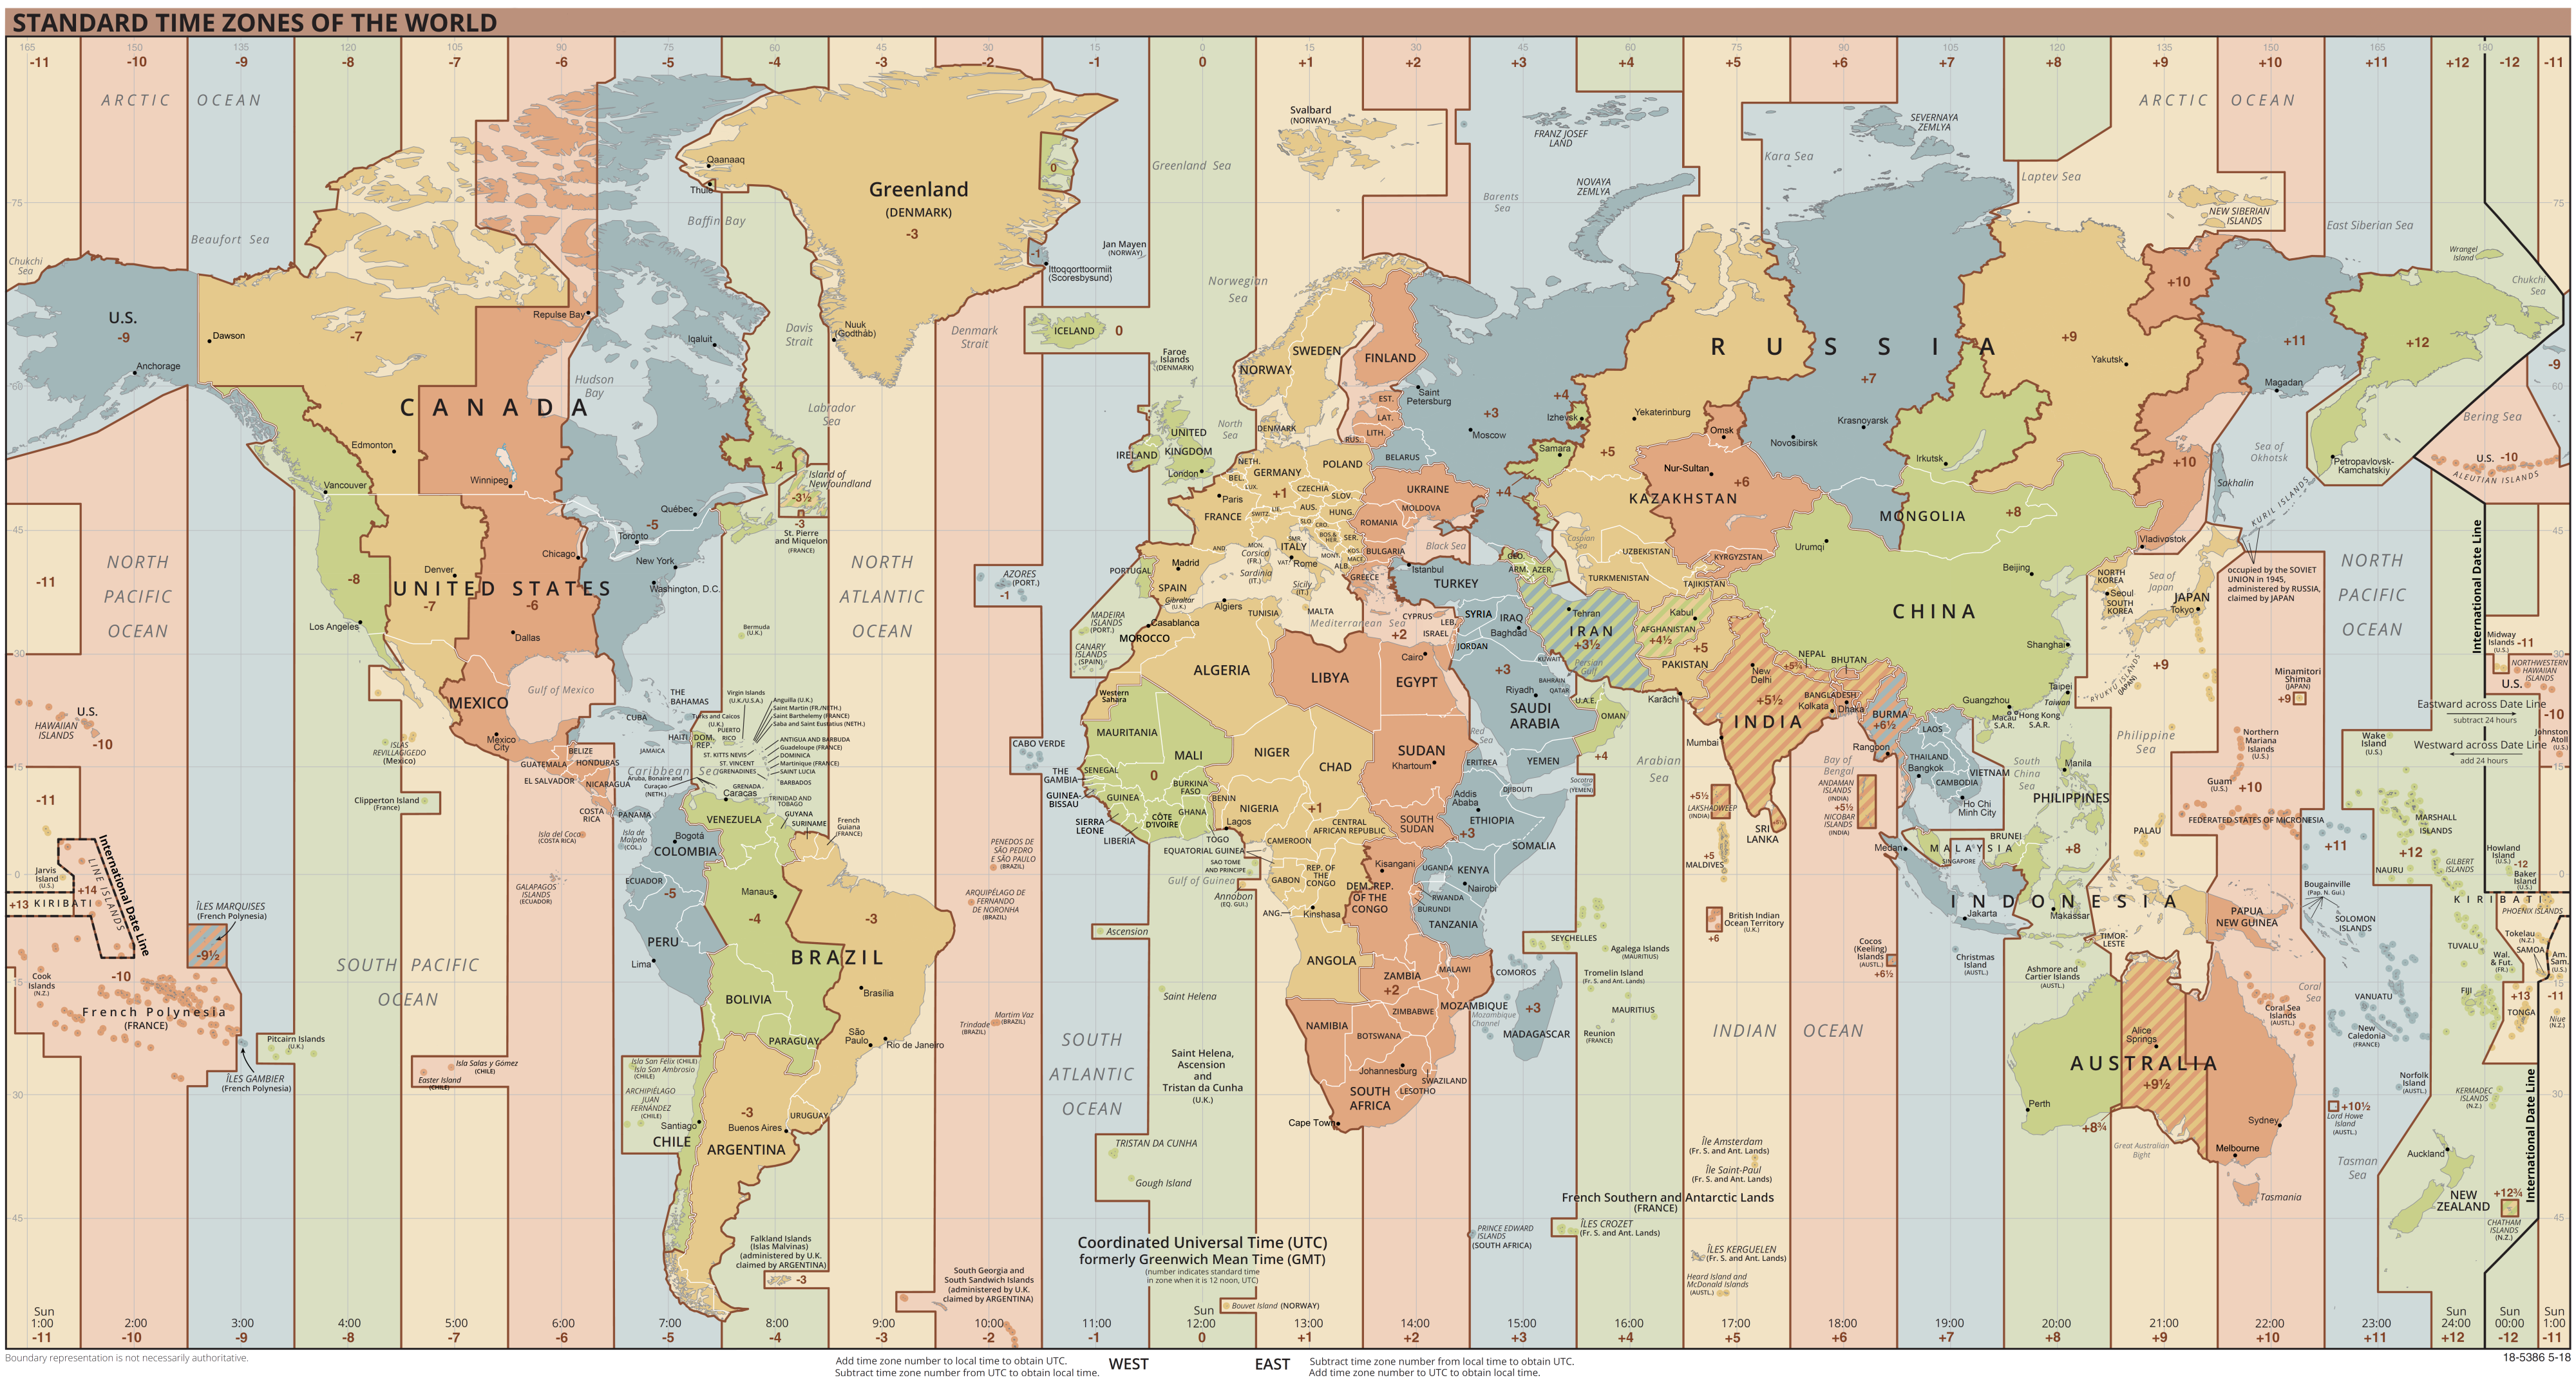
\includegraphics[scale=0.18]{./Bilder/World_Time_Zones_Map.png}
\caption{\label{fig_Zeitzonen}%
Die Zeitzonen der verschiedenen L\"ander. (aus \cite{Wikipedia_Zeitzone})}
\end{figure}

Die Erdkugel ist in 24 Zeitzonen eingeteilt (Abb.\ \ref{fig_Zeitzonen}), jede Zeitzone umfasst 
somit $360/24=15$ L\"angengrade. Befindet sich ein Ort nicht auf dem L\"angengrad seiner Zeitzone, muss 
man pro L\"angengraddifferenz 4 Minuten addieren bzw.\ subtrahieren, je nachdem ob sich der
Ort westlich oder \"ostlich von dem L\"angengrad seiner Zeitzone befindet. Die Mitteleurop\"aische
Zeit, die in Deutschland und den meisten westeurop\"aischen Kontinentalgebieten (au\ss er Portugal)
g\"ultig ist, hat ihren L\"angengrad bei $15^\circ$ Ost. Das ist nahe des
\"ostlichsten Punkts der deutschen Grenze. Selbst Frankfurt an der Oder liegt noch etwas weiter
westlich. Freiburg\index{Freiburg!Zeitzone} 
liegt beim L\"angengrad $7,85^\circ$, also $7,15^\circ$ westlich vom 15.\
L\"angengrad. Dementsprechen muss man zur MEZ rund 28,6 Minuten addieren, um die
wahre Ortszeit zu erhalten (in der Sommerzeit nochmals eine Stunde mehr). Der Sonnenh\"ochstand
im Sommer in Freiburg ist gegen 13:30.   

\subsection{Wahrer und mittlerer Sonnentag}
\label{sec_wahrerSonnentag}

Unabh\"angig von den bisher erw\"ahnten Korrekturen, die zur Bestimmung der lokalen
Ortszeit notwendig sind, kann der wahre Sonnentag, also die Zeitdauer zwischen zwei 
Sonnenh\"ochstst\"anden an einem Ort, im Laufe eines Jahres um bis zu fast einer halben Minute
schwanken, was sich zu manchen Zeiten kumulativ bis zu einer Viertelstunde aufaddieren kann. 
Die beiden Hauptursachen daf\"ur - die elliptische Bahn der Erde und die Neigung der Erdachse 
relativ zur Ekliptik - werden in den Abschnitten \ref{sec_Ellipse} und \ref{sec_Neigung} besprochen. 
Aus diesem Grund definiert man einen mittleren Sonnentag\index{Sonnentag!wahrer} 
als die Dauer eines Tages, sodass ein Jahr\index{Sonnentag!mittlerer}
genau $365,2422$ mittlere Sonnentage hat. Dies hat jedoch zur Folge, dass eine
Uhr, welche die Uhrzeit nach dem mittleren Sonnentag anzeigt, nicht mit einer Uhr \"ubereinstimmt,
welche die wahre Sonnenzeit anzeigt, also z.B.\ eine Sonnenuhr.\index{Sonnenuhr} 
Manche Sonnenuhren
ber\"ucksichtigen diese Effekte, indem die Stundenlinien die Form eines sogenannten
Analemmas haben (Abschnitt \ref{sec_Analemma}).

\section{Zur Mathematik einer elliptischen Bahnkurve}

Es gibt zwei bekannte Definitionen einer Ellipse:\index{Ellipse} 
(1) als die Menge aller Punkte, bei denen die\index{Brennpunkt}
Summe der Abst\"ande zu zwei gegebenen Punkten, den Brennpunkten der Ellipse, konstant ist, 
und (2) als Schnitt
eines Kegelmantels mit einer Ebene. Dass die L\"osungen des Zwei-K\"orper-Kepler-Problems
(also das Zwei-K\"orper-Problem mit einem Potenzial proportional zu $1/r$) Kegelschnitte
sind, ist ebenfalls bekannt. Die gebundenen L\"osungen bilden dabei Ellipsen, wobei 
der Kreis ein Spezialfall einer Ellipse ist. 

Die sogenannte \textit{lineare Exzentrizit\"at} $e$\index{Exzentrizit\"at!lineare} 
einer Ellipse ist gleich dem Abstand vom 
Mittelpunkt der Ellipse zu einem der Brennpunkte. Sie hat die Dimension einer L\"ange. 
Die \textit{numerische Exzentrizit\"at}\index{Exzentrizit\"at!numerische} 
$\epsilon$ ist gleich dem Verh\"altnis von $e$ zur gro\ss en
Halbachse $a$ und ist somit dimensionslos (vgl.\ Abb.\ \ref{fig_ellipse}, links):
\begin{equation}
\label{eq_fracea}
               \epsilon = \frac{e}{a} \, .
\end{equation}
Au\ss erdem gilt
\begin{equation}
\label{eq_zweia}
             2a = r_{\rm max} + r_{\rm min}  \hspace{1cm} {\rm und} \hspace{1cm}
             2e = r_{\rm max} - r_{\rm min}   \, ,
\end{equation}
wobei $r_{\rm max}$ der maximale Abstand zwischen einem Brennpunkt und der Ellipse ist (also der
Abstand zwischen einem Brennpunkt und dem gegen\"uberliegenden Punkt der Ellipse) und $r_{\rm min}$
der minimale Abstand. Bei der Erdumlaufbahn um die Sonne bezeichnet man den Punkt mit dem
maximalen Abstand zur Sonne als Aphel,\index{Aphel}\index{Perihel} 
den Punkt mit dem minimalen Abstand als Perihel.\footnote{Bei der Mondbahn 
um die Erde bezeichnet man den Punkt der Mondbahn mit dem gr\"o\ss ten 
Abstand zur Erde als Apog\"aum\index{Apog\"aum}\index{Perig\"aum} 
und den Punkt mit dem kleinsten Abstand als Perig\"aum.} 
 
Aus den Gleichungen \ref{eq_fracea} und \ref{eq_zweia} folgt
\begin{equation}
               \epsilon = \frac{r_{\rm max} - r_{\rm min}}{r_{\rm max} + r_{\rm min}}
               \hspace{1cm}  {\rm oder}  \hspace{1cm}   \frac{r_{\rm min}}{r_{\rm max}} = 
               \frac{1-\epsilon}{1+\epsilon}         \, .
\end{equation}

\begin{figure}[htb]
\setlength{\unitlength}{0.8pt}
\begin{picture}(250,150)(8,0)
\qbezier(8.5,75)(9,107)(50,130)
\qbezier(50,130)(80,145)(125,146)
\qbezier(8.5,75)(9,43)(50,20)
\qbezier(50,20)(80,5)(125,4)
\qbezier(241.5,75)(241,107)(200,130)
\qbezier(200,130)(170,145)(125,146)
\qbezier(241.5,75)(241,43)(200,20)
\qbezier(200,20)(170,5)(125,4)
\put(53,75){\makebox(0,0){$\bullet$}}
\put(125,146){\makebox(0,0){$\bullet$}}
\put(197,75){\makebox(0,0){$\bullet$}}
\put(125,75){\makebox(0,0){$\bullet$}}
\put(8.5,75){\line(1,0){116.5}}
\put(125,75){\line(1,0){116.5}}
\put(53,75){\line(1,1){70}}
\put(197,75){\line(-1,1){70}}
\put(160,120){\makebox(0,0){$a$}}
\put(160,80){\makebox(0,0){$e$}}
%
\qbezier(8.5,73)(8.5,70)(20,70)
\qbezier(20,70)(31.5,70)(31.5,67)
\qbezier(31.5,67)(31.5,70)(43,70)
\qbezier(43,70)(53,70)(53,73)
\qbezier(53,73)(53,55)(120,55)
\qbezier(120,55)(150,55)(150,50)
\qbezier(150,50)(150,55)(180,55)
\qbezier(180,55)(241.5,55)(241.5,73)
\qbezier(125,73)(125,70)(153,70)
\qbezier(153,70)(180,70)(180,65)
\qbezier(180,65)(180,70)(207,70)
\qbezier(207,70)(241.5,70)(241.5,73)
\put(31.5,62){\makebox(0,0){$r_{\rm min}$}}
\put(150,45){\makebox(0,0){$r_{\rm max}$}}
\put(180,60){\makebox(0,0){$a$}}
\end{picture}
\hfill
\begin{picture}(270,150)(0,0)
\qbezier(8.5,75)(9,107)(50,130)
\qbezier(50,130)(80,145)(125,146)
\qbezier(8.5,75)(9,43)(50,20)
\qbezier(50,20)(80,5)(125,4)
\qbezier(241.5,75)(241,107)(200,130)
\qbezier(200,130)(170,145)(125,146)
\qbezier(241.5,75)(241,43)(200,20)
\qbezier(200,20)(170,5)(125,4)
\put(53,75){\makebox(0,0){$\bullet$}}
%\put(125,146){\makebox(0,0){$\bullet$}}
%\put(197,75){\makebox(0,0){$\bullet$}}
%\put(125,75){\makebox(0,0){$\bullet$}}
\put(8.5,73){\vector(0,-1){0}}
\put(241.5,77){\vector(0,1){0}}
\put(53,75){\line(-1,0){45}}
\put(53,75){\line(-2,-1){40}}
\put(53,75){\line(1,0){190}}
\qbezier(53,75)(147,80)(240,85)
%\qbezier(53,75)(147,70)(240,65)
\put(-9,75){\makebox(0,0){$v_{\rm max}$}}
\put(258,75){\makebox(0,0){$v_{\rm min}$}}
%
\put(55,55){\makebox(0,0){${\scriptstyle \alpha_{\rm max}}$}}
\put(55,60){\vector(-1,1){13}}
\qbezier(35,75)(35,70)(37,68)
\put(70,95){\makebox(0,0){${\scriptstyle \alpha_{\rm min}}$}}
\put(75,89.5){\vector(1,-1){13}}
\qbezier(120,75)(120,76)(119.5,79)
\put(33,81){\makebox(0,0){$r_{\rm min}$}}
\put(170,69){\makebox(0,0){$r_{\rm max}$}}
\end{picture}
\caption{\label{fig_ellipse}%
(links) Die geometrischen Gr\"o\ss en in einer Ellipse: $a$ (gro\ss e Halbachse), $e$ (Exzentrizit\"at),
$r_{\rm min}$ und $r_{\rm max}$ (kleinster und gr\"o\ss ter Abstand der Ellipse zu einem Brennpunkt);
(rechts) die dynamischen Gr\"o\ss en in einer Ellipse: $v_{\rm min}$ und $v_{\rm max}$ (kleinste und
gr\"o\ss te Geschwindigkeit eines umlaufenden Objekts), $\alpha_{\rm max}$ und $\alpha_{\rm min}$ 
(in gleichen Zeiten \"uberstrichene Winkel im Perihel und Aphel).}
\end{figure}

Nach dem zweiten\index{Kepler'sches Gesetz!zweites} 
Kepler'schen Gesetz (\glqq In gleichen Zeiten werden gleiche Fl\"achen \"uberstrichen\grqq)
folgt, dass sich die Geschwindigkeiten im Perihel (dem sonnenn\"achsten Punkt), $v_{\rm max}$, 
zur Geschwindigkeit im Aphel (dem sonnenfernsten Punkt), $v_{\rm min}$, wie die Abst\"ande der Bahn
zur Sonne verhalten (siehe Abb.\ \ref{fig_ellipse}, rechts):
\begin{equation}
                 \frac{v_{\rm min}}{v_{\rm max}} =  \frac{r_{\rm min}}{r_{\rm max}}   \, .
\end{equation} 
Das zweite Kepler'sche Gesetz\index{Drehimpulserhaltung} 
ist \"aquivalent zur Drehimpulserhaltung.\hyperref[sec_Zeitgleichung_A]{(Herleitung)}

F\"ur die Winkel im Perihel $\alpha_{\rm max}$ und Aphel $\alpha_{\rm min}$, 
die in gleichen Zeiten \"uberstrichen werden, bedeutet dies:
\begin{equation}
\label{eq_maxzumin}
      \frac{\alpha_{\rm min}}{\alpha_{\rm max}} 
      = \left( \frac{v_{\rm min}}{r_{\rm max}} \right) \Big/ \left( \frac{v_{\rm max}}{r_{\rm min}} \right) 
                 = \left( \frac{r_{\rm min}}{r_{\rm max}} \right)^2 \, .
\end{equation} 

\section{Der Einfluss der elliptischen Bahnkurve}
\label{sec_Ellipse}

In diesem Abschnitt vernachl\"assigen wir die Neigung der Erdachse zur Ekliptik (diesen
Effekt ber\"ucksichtigen wir im n\"achsten Abschnitt) und nehmen an, die Rotationsachse
der Erde sei senkrecht zu ihrer Bahnebene. 

W\"urde sich die Erde auf einer Kreisbahn um die Sonne bewegen, w\"are der Winkel, den
sie auf ihrer Bahn um die Sonne t\"aglich \"uberstreicht, immer derselbe. Wir bezeichnen diesen Winkel
mit $\alpha_0$. Sein Wert berechnet sich aus der Tatsache, dass ein Jahr rund $365,2422$ Tage
dauert und in dieser Zeit ein Winkel von $360^\circ$ \"uberstrichen wird:
\begin{equation}
                \alpha_0 = \frac{360^\circ}{365,2422\,{\rm d}} = 0,98565^\circ/{\rm d} \, . 
\end{equation} 
Die Erde dreht sich in 24 Stunden einmal um ihre Achse von Sonnenh\"ohststand zu
Sonnenh\"ochstand. Dabei \"uberstreicht sie einen Winkel von 
$360^\circ + \alpha$. Der zus\"atzliche Winkel $\alpha$ r\"uhrt daher, dass sich die Erde im
Verlauf eines Tages auf ihrer Bahn weiter um die Sonne bewegt hat, und sich somit
die Sonne relativ zur Erde um den Winkel $\alpha$ weiterbewegt hat. Auf einer
Kreisbahn w\"are dieser Winkel $\alpha=\alpha_0$. Um sich um diesen Winkel $\alpha$
zu drehen, ben\"otigt sie ungef\"ahr 4 Minuten.\footnote{Da sich die Erde in 24 Stunden um
rund $360^\circ$ dreht, dreht sie sich in einer Stunde um $15^\circ$ und somit in 4 Minuten
um $1^\circ$.} 
Um diese Zeit ist der ideale Sonnentag\index{Tag!siderischer}
l\"anger als der siderische Tag (der sich auf eine Umdrehung relativ zum Fixsternhimmel bezieht).

Tats\"achlich bewegt die Erde sich aber auf einer elliptischen Bahn und ihre Winkelgeschwindigkeit
ist im Perihel gr\"o\ss er als im Aphel. Das bedeutet, dass an einem Tag in Periheln\"ahe (dieser Tag
liegt derzeit um den 3.\ Januar) ein gr\"o\ss erer Winkel von ihr relativ zur Sonne \"uberstrichen wird
als an einem Tag im Aphel (rund 3. Juli). F\"ur die Zeitabh\"angigkeit dieses Winkels k\"onnen wir
folgenden Ansatz machen
\begin{equation}
\label{eq_alphat}
                \alpha(t) = \alpha_0 \left( 1 + A \cos \left( \frac{2\pi}{T} t \right) \right)  \, , 
\end{equation} 
wobei $T$ die Periodendauer der Erdbahn um die Sonne ist - also ein Jahr -
und die Zeit $t$ am Perihel beginnen soll (also $\alpha(t=0)=\alpha_{\rm max}$). 
Nach Gl.\ \ref{eq_maxzumin} besteht folgende Beziehung zwischen der Amplitude $A$ und
der Exzentrizit\"at $\epsilon$: 
\begin{equation}
               \frac{\alpha_{\rm max}}{\alpha_{\rm min}} = \left( \frac{  1 + \epsilon}{1-\epsilon} \right)^2
              \approx 1+4\epsilon  \, . 
\end{equation} 
Andererseits gilt nach Gl.\ \ref{eq_alphat}:
\begin{equation}
               \frac{\alpha_{\rm max}}{\alpha_{\rm min}} =
            \frac{\alpha(0)}{\alpha(T/2)} = \frac{ \alpha_0 ( 1 + A )}{\alpha_0(1-A)} 
            \approx 1 + 2A  \, . 
\end{equation} 
Wir erhalten somit die Beziehung $A = 2 \epsilon$. 

F\"ur die Winkelgeschwindigkeit der Eigendrehung der Erde k\"onnen wir nach obiger
Argumentation schreiben:
\begin{equation}
             \omega = \frac{360^\circ + \alpha_0}{86400\,{\rm s}} \, .
\end{equation}
Andererseits ist die Zeitdauer $T(\alpha)$, die die Erde ben\"otigt, um sich um den Winkel
$\alpha$ zu drehen, gegeben durch
\begin{equation}
             T(\alpha)  = \frac{\alpha}{\omega}     \, , 
\end{equation} 
und damit dauert ein Tag (in Abh\"angigkeit von der Jahreszeit $t$):
\begin{eqnarray}
              T(t) &=& \frac{360^\circ + \alpha(t)}{\omega} 
              = \left( \frac{360^\circ + 
                   \alpha_0( 1 + 2 \epsilon \cos \frac{2\pi}{T}t)}{360^\circ + \alpha_0}\right)  T_0 \\
              &=& T_0 + 2 \alpha_0 \epsilon \frac{\cos  \frac{2\pi}{T}t}{360^\circ + \alpha_0} T_0  \, ,
\end{eqnarray} 
wobei $T_0=86\,400$\,s einem mittleren Sonnentag entspricht.
Die Zeitdifferenz zwischen einem mittleren Sonnentag und dem tats\"achlichen Sonnentag ist
somit
\begin{equation}
\label{eq_Zeitdifferenz}
              \Delta T(t) = T(t)-T_0 =  2 \alpha_0 \epsilon \frac{\cos  \frac{2\pi}{T}t}{360^\circ + \alpha_0}T_0   \, .
\end{equation} 
Setzen wir Werte ein, so erhalten wir f\"ur die Amplitude dieser Schwankung:
\begin{equation}
              \Delta T =  2 \alpha_0 \epsilon \frac{1}{360^\circ + \alpha_0} 86400\,{\rm s} \approx 
                7,88\,{\rm s}   \, .
\end{equation} 
Um diesen Wert kann ein einzelner Tag also l\"anger oder k\"urzer sein als ein mittlerer Sonnentag (sofern
man nur die elliptische Bahn der Erde ber\"ucksichtigt). Ein solcher Effekt f\"ur sich genommen w\"are vermutlich
im Altertum noch nicht aufgefallen, w\"are dieser Effekt nicht kumulativ, d.h., wenn viele aufeinanderfolgende
Tage um \"ahnliche Werte zu lang oder zu kurz sind, addieren sich die Effekte auf. Je nach Jahreszeit
geht die tats\"achliche
Zeit der gemittelten Zeit voraus bzw.\ nach. Relevant f\"ur die Zeitgleichung ist dieser kumulative
Effekt, d.h.\ die Differenz zwischen der wahren Zeit, die an einem Ort am Stand der Sonne abgelesen 
wird, und der gemittelten Zeit, die eine Uhr anzeigt. 

Bilden wir von Gl.\ \ref{eq_Zeitdifferenz} die Summe, erhalten wir:
\begin{equation}
     {\rm ZG}_1(t) = \sum_{t'=0}^t \Delta T(t')  \approx  \frac{T}{2\pi} \Delta T \sin \frac{2\pi}{T}t  \, .
\end{equation}
Hierbei verl\"auft die Summe \"uber die Tage $t$ vom Perihel gerechnet und $T$ ist die Dauer eines
Jahres in Tagen (also $T=365,2422$). Die Summe selbst wurde durch ein Integral approximiert. 
Die Amplitude dieser periodischen Funktion ist schon betr\"achtlich h\"oher: Sie betr\"agt rund
$7,63$ Minuten. Dies ist ein Ma\ss\ f\"ur den kumulativen Effekt: Im Verlauf eines Jahres kann die
wahre Zeit an einem Ort der gemittelten Zeit um $\pm 7,63$ Minuten vor bzw.\ nach gehen. 
Dieser Effekt ist Anfang April (drei Monate nach dem Perihel) und nochmals Anfang Oktober (sechs
Monate sp\"ater) am gr\"o\ss ten. Zun\"achst hinkt die wahre Zeit der gemittelten Zeit hinterher. 

\section{Die Neigung der Erdachse zur Ekliptik}
\label{sec_Neigung}

F\"ur\index{Neigung, Erdachse zur Ekliptik} 
die separate Beschreibung des zweiten Einflusses auf die Tagesl\"ange nehmen wir an, dass sich
die Erde gleichm\"a\ss ig auf einer Kreisbahn um die Sonne bewegt. Wir ber\"ucksichtigen allerdings
nun, dass die Rotationsachse der Erde um $23,44^\circ$ relativ zur Normalen der Ekliptik (der Bahnebene 
der Erde) geneigt ist. Au\ss erdem ist es sinnvoll, nicht ein heliozentrisches Koordinatensystem
zu verwenden, sondern ein geozentrisches, allerdings soll dieses Koordinatensystem relativ zum
Fr\"uhlingspunkt (also der Schnittlinie zwischen \"Aquatorebene und Ekliptik) fest sein 
(siehe Abb.\ \ref{fig_Ekliptik}). 
Die $z$-Achse dieses Sys\-tems sei die Rotationsachse der Erde, die $x,y$-Achsen liegen dann in
der \"Aquatorebene (z.B.\ sei die $x$-Achse die Schnittlinie der Ekliptik und \"Aquatorebene, sie
zeige also in Richtung Fr\"uhlingspunkt). Es handelt sich also nicht um ein erdfestes
Koordinatensystem, das die t\"agliche Drehung der Erde mitmacht, sondern um ein Koordinatensystem,
das bez\"uglich des Fr\"uhlingspunkts fest ist. Dies ist auch das Koordinatensystem, das man
in der Astronomie h\"aufig verwendet. 

\begin{SCfigure}[30][htb]
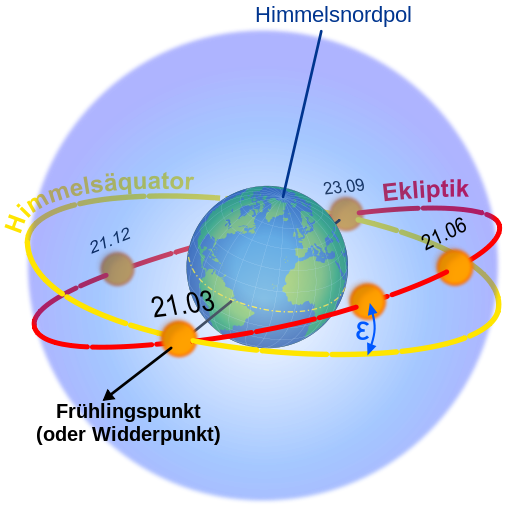
\includegraphics[scale=0.3]{./Bilder/Ecliptic.png}
\caption{\label{fig_Ekliptik}%
\"Aquatorebene und Ekliptik sind um $23,44^\circ$ gegeneinander geneigt (hier mit
$\varepsilon$ bezeichnet). Eine
gleichm\"a\ss ige Bewegung der Sonne entlang der Ekliptik wird zu einer
ungleichm\"a\ss igen Bewegung in Bezug auf die L\"angengrade.} 
\end{SCfigure}

In Bezug auf ein solches Koordinatensystem bewegt sich die Sonne im Verlauf eines Jahres
gleichf\"ormig auf einem Kreis, der um $23,44^\circ$ relativ zur \"Aquatorebene geneigt ist. 
Die Gleichf\"ormigkeit dieser Bewegung folgt aus der gleichf\"ormigen Bewegung der Erde um
die Sonne (da wir eine Kreisbewegung annehmen). Die L\"angengrade auf der Erde schneiden
die scheinbare Bahn der Sonne, die relativ zum \"Aquator geneigt ist, jedoch nicht gleichf\"ormig.
Das bedeutet, dass die scheinbare Bewegung der Sonne relativ zu den L\"angengraden
nicht gleichf\"ormig ist, und das wiederum bedeutet, dass ein Sonnentag zu manchen Zeiten
k\"urzer bzw.\ l\"anger ist. Genauer sind die Tage um den Fr\"uhlings- und Herbstpunkt die
k\"urzesten und die Tage um die Sommer- und Wintersonnenwende die l\"angsten.  
 
Zur Berechnung dieses Effekts f\"ur die Zeitgleichung 
muss man einen gleichm\"a\ss ig unterteilten Vollkreis, der unter $23,44^\circ$ geneigt ist,
entlang der L\"angengrade auf die \"Aquatorebene projizieren. 
Die auf der Ekliptik gleichen\index{Sommersonnenwende}\index{Wintersonnenwende}
Bogenl\"angen werden auf der \"Aquatorebene ungleich - etwas dichter am Fr\"uhlingspunkt (derzeit
21.3.) und Herbstpunkt (derzeit 23.9.) und etwas weniger dicht bei der Sommersonnenwende
(derzeit 21.6.) und der Wintersonnenwende 
(derzeit 21.12).\index{Fruehlingspunkt@Fr\"uhlingspunkt}\index{Herbstpunkt}      
   
\begin{figure}[htb]
\begin{picture}(200,100)(0,0)
\put(135,54){\makebox(0,0){${\scriptstyle 23,44^\circ}$}}
\put(175,75){\makebox(0,0){$\bullet$}}
\put(175,50){\makebox(0,0){$\bullet$}}
\put(100,50){\makebox(0,0){$\bullet$}}
\put(145,73){\makebox(0,0){$a$}}
\put(147,43){\makebox(0,0){$a'$}}
\put(50,20){\makebox(0,0){\footnotesize Ekliptik}}
\put(30,57){\makebox(0,0){\footnotesize \"Aquator}}
\put(160,15){\makebox(0,0){\footnotesize L\"angengrad}}
\put(175,20){\line(0,1){70}}
\put(100,20){\line(0,1){70}}
\qbezier(148,66)(150,60)(150,50)
\thicklines
\put(10,50){\line(1,0){180}}
\put(10,20){\line(3,1){180}}
\end{picture}
\hfill
%
\begin{picture}(210,100)(0,0)
\put(190,20){\makebox(0,0){${\scriptstyle 0^\circ}$}}
\put(185,85){\makebox(0,0){${\scriptstyle 23,44^\circ}$}}
\put(45,20){\makebox(0,0){$\bullet$}}
\put(155,20){\makebox(0,0){$\bullet$}}
\put(50,81){\makebox(0,0){$\bullet$}}
\put(150,81){\makebox(0,0){$\bullet$}}
\put(100,77){\makebox(0,0){$a$}}
\put(100,27){\makebox(0,0){$a'$}}
\put(10,83){\line(1,0){160}}
\qbezier(52,95)(45,60)(45,20)
\qbezier(148,95)(155,60)(155,20)
\put(25,72){\makebox(0,0){\footnotesize Ekliptik}}
\put(30,13){\makebox(0,0){\footnotesize \"Aquator}}
\put(180,50){\makebox(0,0){\footnotesize L\"angengrad}}
\thicklines
\put(10,20){\line(1,0){170}}
\qbezier(10,80)(100,85)(190,80)
\end{picture}
\caption{\label{fig_ZGProj}%
Projektionen von der Ekliptik auf die \"Aquatorebene in der N\"ahe der \"Aquinoktien (Schnittpunkte
zwischen \"Aquator und Ekliptik; links) und der Sommer- bzw.\ Wintersonnenwende (rechts). Zwei Punkte,
die entlang der Ekliptik eine Bogenl\"ange $a$ haben, werden entlang der L\"angengrade auf zwei
Punkte auf dem \"Aquator projiziert, die dort eine Bogenl\"ange $a'$ haben. Man vergleiche diese
Abbildung auch mit Abb.\ \ref{fig_Hondius1} und \ref{fig_Hondius2}.}
\end{figure}   
   
Die folgende Herleitung dieses Beitrags geht davon aus, dass sich der Effekt wieder als
eine trigonmetrische Funktion schreiben l\"asst, was in guter N\"aherung auch erf\"ullt ist. 
Diese Funktion hat im Verlaufe eines Jahres zwei Maxima (an den Sonnenwenden) und zwei
Minima (an den \"Aquinoktien). Damit m\"ussen wir nur noch die Amplitude dieser Funktion
bestimmen.   

Wie aus Abb.\ \ref{fig_ZGProj} ersichtlich, \"andert sich eine Bogenl\"ange $a$, wenn sie von der
Ekliptik entlang der L\"angengrade auf den \"Aquator projiziert wird. In der N\"ahe der
\"Aquinoktien ist die Beziehung durch $a'= a \cos \varepsilon$ gegeben. In der N\"ahe der
Sonnenwendepunkte am $23,44$.ten Breitengrad gilt ungef\"ahr 
\mbox{$a=a' \cos \varepsilon$} (genauer
ist dies die Beziehung zwischen den Bogenl\"angen entlang der beiden Breitengrade; der
Abstand zwischen den beiden Punkten entlang der Ekliptik ist etwas kleiner, dies kann man aber
in f\"uhrender Ordnung und wenn die Punkte gen\"ugend nahe beieinander liegen vernachl\"assigen).   
Machen wir wieder einen Ansatz der Form
\begin{equation}
                \alpha(t) = \alpha_0 \left( 1 + B \cos \left( \frac{4 \pi}{T} t \right) \right) 
\end{equation}
folgt   
\begin{equation}
                \frac{\alpha_{\rm min}}{\alpha_{\rm max}}  
                =  \frac{ 1 - B}{1+B} = \cos^2 \varepsilon  
\end{equation}
oder
\begin{equation}
               B =  \frac{ 1 - \cos^2 \varepsilon }{1+\cos^2 \varepsilon } =  0,0859153\, . 
\end{equation}
Dies f\"uhrt auf maximale Schwankungen in der Tagesl\"ange von $\pm 20,27$\,s und auf
eine kumulative Zeitverschiebung von 
\begin{equation}
     {\rm ZG}_2(t) = \sum_{t=0}^t \Delta T(t)  \approx  \frac{T}{4\pi} \Delta T \sin \frac{4\pi}{T}t  
                    \approx (9,82\,{\rm min})\cdot \sin \frac{4\pi}{T}t  \, .
\end{equation}
Wiederum ist $T$ die Zeitdauer von einem Jahr, und da in der Summe die Diskretisierung
in Tagen $t$ vorgenommen wurde, sollte auch $T$ in Tagen angegeben werden. 
$t$ ist die Anzahl der Tage vom Fr\"uhlingspunkt (dort ist nun $t=0$) gemessen.

\section{Die Zeitgleichung}

Die Zeitgleichung ist die Summe dieser beiden Beitr\"age. Dabei ist noch zu ber\"ucksichtigen,
dass die Zeitpunkte $t=0$ unterschiedlich gew\"ahlt wurden. Gibt man $t$ in Tagen an, sollte
die Periode f\"ur den ersten Anteil (elliptische Erdbahn) am 3.\ Januar beginnen, also am 3.\ Tag
des Jahres, und die Periode f\"ur den zweiten Anteil (Neigung der Erdachse zur Ekliptik) am
21.\ M\"arz, in Jahren, die kein Schaltjahr sind, also am 80.\ Tag eines Jahres. 
Abb.\ \ref{fig_Zeitgleichung} zeigt die Summe der beiden Beitr\"age.

\begin{SCfigure}[30][htb]
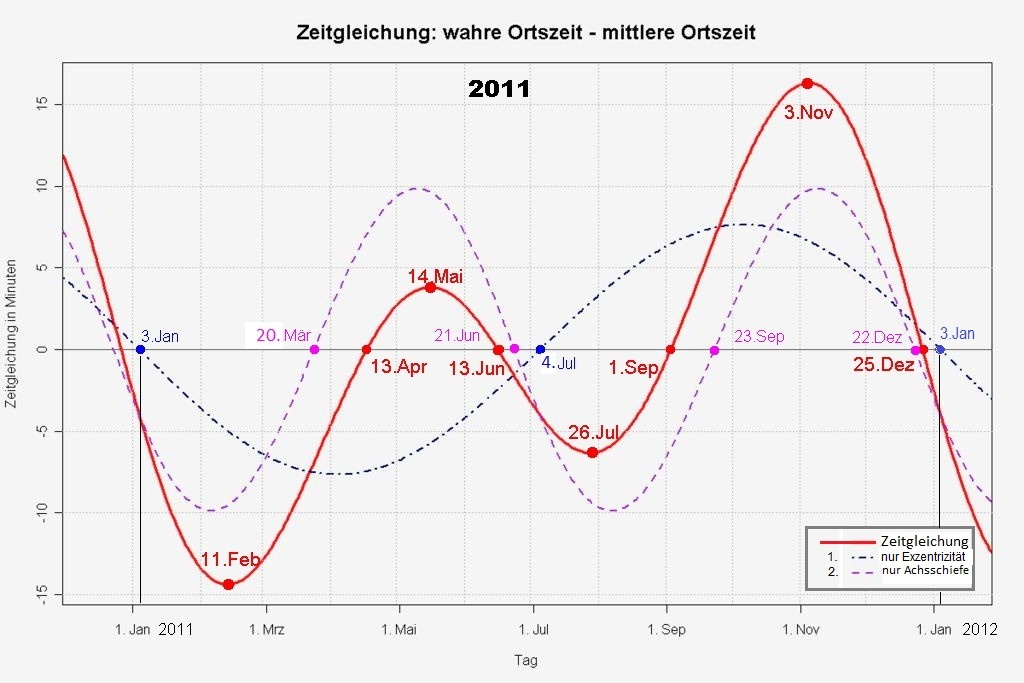
\includegraphics[scale=0.36]{./Bilder/Zeitgleichung.jpg}
\caption{\label{fig_Zeitgleichung}%
Die Zeitgleichung. Im Verlaufe eines Jahres kann die wahre Ortszeit von der mittleren Ortszeit
um \"uber eine Viertelstunde abweichen. Da sich das Perihel langsam verschiebt (in rund 21\,000 Jahren
einmal um $360^\circ$) verschieben sich im Verlauf der Zeit auch die beiden Beitr\"age relativ zueinander.
(aus \cite{Wikipedia_Zeitgleichung})} 
\end{SCfigure}

Insgesamt sind die Minuten der Zeitgleichung zur wahren Ortszeit zu addieren, sodass man die
mittlere Ortszeit erh\"alt. Diese Wahl des Vorzeichens geht darauf zur\"uck, dass man fr\"uher
beispielsweise mithilfe eines Sextanten auf hoher See die wahre Ortszeit gemessen hat
und nun die mittlere Ortszeit berechnen musste. 
Ist die Zeitgleichung negativ (beispielsweise zu Beginn des Jahres) m\"ussen die 
entsprechenden Minuten (Absolutwerte) der Zeitgleichung also von der wahren Ortszeit 
abgezogen werden, um zur mittleren Ortszeit zu gelangen. 

\section{Kuriosit\"aten}
\subsection{Die Ekliptik auf alten Landkarten und Globen}

Auf manchen alten Landkarten und Globen ist die Projektion der Ekliptik auf die
Erde eingezeichnet. Ein Beispiel ist die bekannte Weltkarte von\index{Hondius, Hendrik} 
Hendrik Hondius aus dem
Jahr 1630 (Abb.\ \ref{fig_Hondius}, oben).

\begin{figure}[p]
\includegraphics[scale=0.44]{./Bilder/Hondius_gesamt.png}\\[0.2cm]
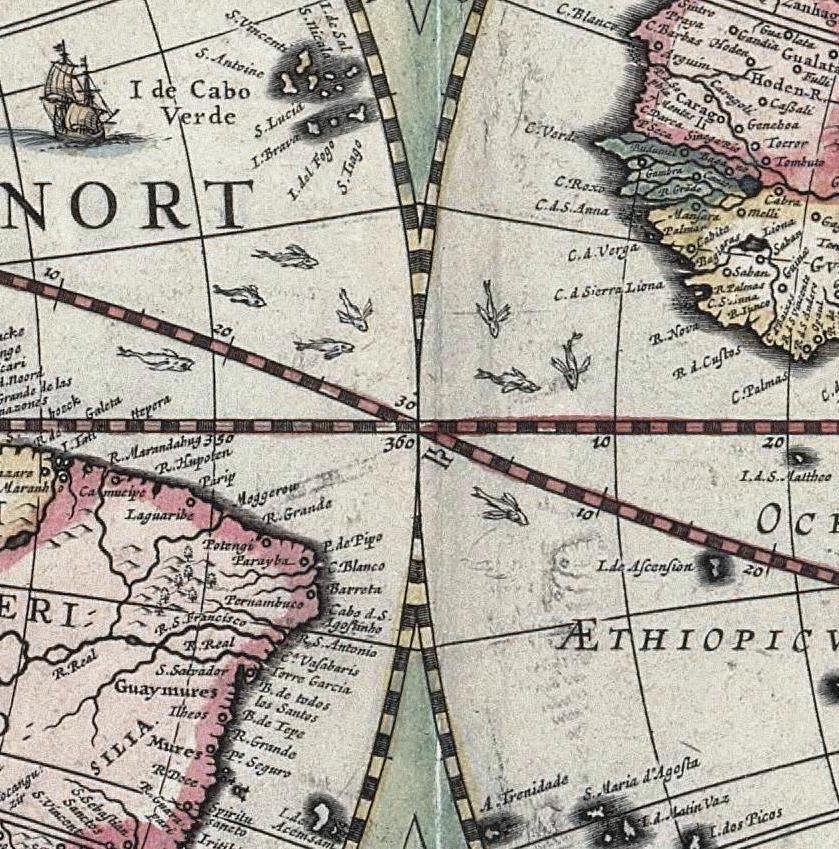
\includegraphics[scale=0.2]{./Bilder/Hondius_00.jpg} \hfill
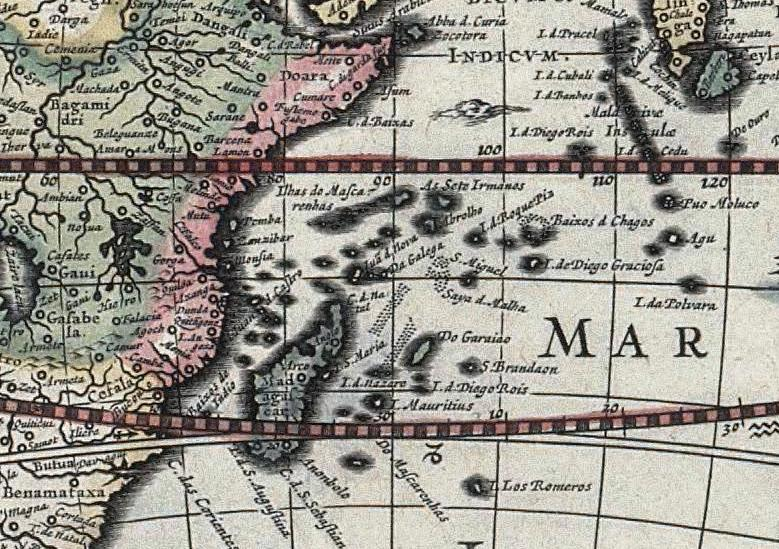
\includegraphics[scale=0.31]{./Bilder/Hondius_90.jpg}
\caption{\label{fig_Hondius}%
(Oben) Weltkarte von Hendrik Hondius aus dem Jahr 1630. Deutlich erkennbar neben der
\"Aquatorlinie ist die Projektion der Ekliptik. (Unten)
Ausschnitte aus der Weltkarte von Hendrik Hondius. (links) Ausschnitt beim Schnittpunkt von 
\"Aquator und Ekliptik, der hier auf einen der damals gebr\"auchlichen Nullmeridiane durch die
Azoren gelegt wurde. Links unten sind Teile von S\"udamerika erkennbar, rechts oben Teile von
Afrika. (rechts) Ausschnitt in der N\"ahe des s\"udlichen Wendepunkts der Ekliptik (unser
Winterpunkt). Der Kontinent links ist Afrika, die Insel rechts daneben Madagaskar; rechts oben
erkennt man die S\"udspitze von Indien und Sri Lanka (damals Ceylon). (\cite{Puzzle})}
\end{figure}

Sowohl die \"Aquatorlinie als auch die Ekliptik sind in $360$ \"aquidistante Einheiten von
jeweils $1^\circ$ unterteilt. F\"ur die \"Aquatorlinie gilt das auch auf der Karte. Da der Gro\ss kreis
der Ekliptik in seiner Projektion auf der Karte bei unterschiedlichen Breitengraden verl\"auft und
der Ma\ss stab der Karte vom Breitengrad abh\"angt (siehe auch Kap.\ \ref{chap_Landkarte}),
erscheint die Unterteilung der Ekliptik nicht mehr gleichf\"ormig.
In der N\"ahe der Wendepunkten der Sonne, also in den Bereichen, wo die
Ekliptik in der N\"ahe des $\pm 23,5$.\ Breitengrads ist, sind die Unterteilungen auf der Ekliptik etwas
breiter als am \"Aquator (siehe Abb.\ \ref{fig_Hondius}, unten rechts), da der Ma\ss stab auf der Karte kleiner
wird, wenn man sich vom \"Aquator entfernt. In den Ausschnitten (Abb.\ \ref{fig_Hondius}, unten)
erkennt man, dass beim Schnittpunkt der Ekliptik mit dem \"Aquator (also den \"Aquinoktien) die
Projektion der Ekliptik auf den \"Aquator die Bogenl\"ange schrumpfen l\"asst (Abb.\ \ref{fig_Hondius}, unten links).
An diesen Stellen schneidet die $10^\circ$ Bogenl\"ange der Ekliptik den \"Aquator links von der
$10^\circ$ Marke bzw.\ dem 10.\ L\"angengrad. Andererseits vergr\"o\ss ert
wegen des ver\"anderten Ma\ss stabs die Projektion entlang der L\"angengrade in der
N\"ahe der Wendepunkte die Bogenl\"ange (Abb.\ \ref{fig_Hondius}, unten rechts): Hier liegt die
$10^\circ$ Marke der Ekliptik ($10^\circ$ neben dem Wendepunkt) rechts neben dem 100.\ L\"angengrad
(der 90.\ L\"angengrad markiert den Wendepunkt) am \"Aquator. 

\subsection{Das Analemma}
\label{sec_Analemma}

Das Analemma\index{Analemma} 
ist eine achtf\"ormige Figur, die ungef\"ahr den Schattenverlauf der Spitze
eines Stabes (z.B.\ eines Obelisken oder der Spitze des Zeigers einer Sonnenuhr) zur
selben mittleren Ortszeit (z.B.\ um 12 Uhr mittags) im Verlauf eines Jahres beschreibt (siehe
Abb.\ \ref{fig_Analemma}, links). 
Die beiden Koordinaten dieser Figur entsprechen einmal dem unterschiedlichen H\"ochstand
der Sonne im Sommer und Winter: Im Winter steht die Sonne auch zur Mittagszeit sehr tief
und somit ist der Schatten vergleichsweise lang, im Sommer steht die Sonne hoch am
Himmel und daher ist der Schatten entsprechend kurz. 

\begin{figure}[htb]
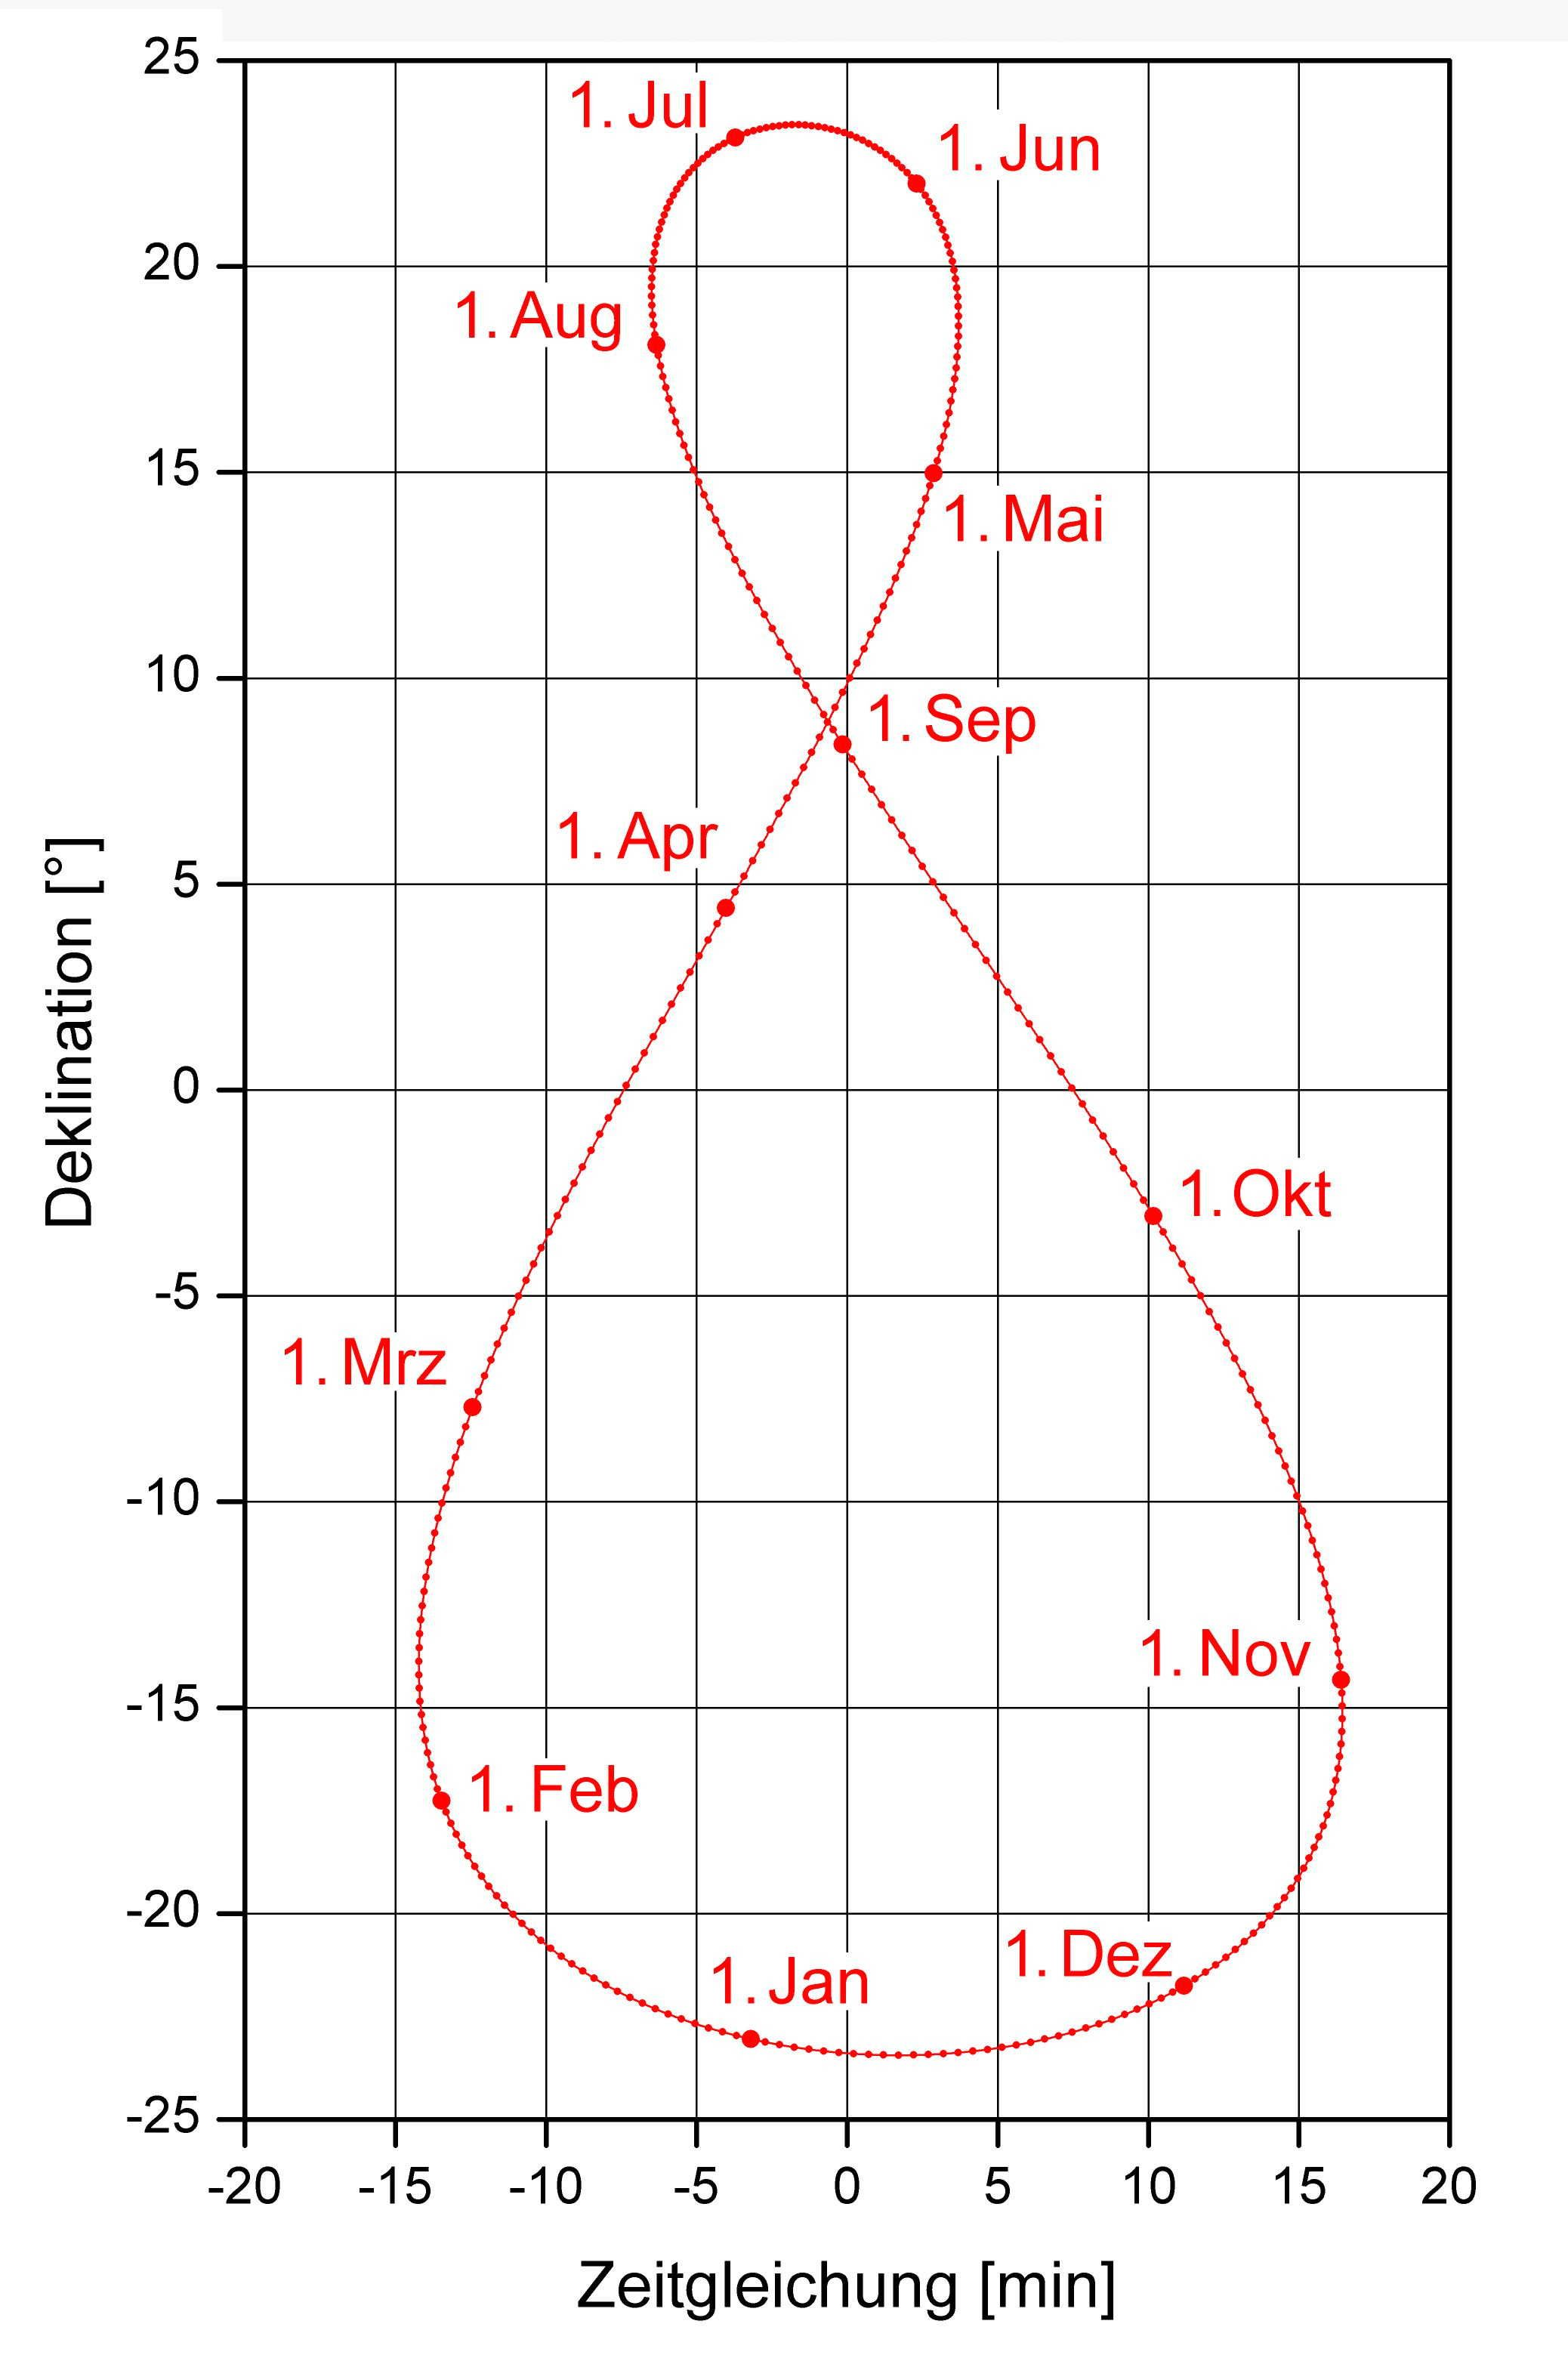
\includegraphics[scale=0.28]{./Bilder/Analemma.jpg} 
\hfill
\includegraphics[scale=0.24]{./Bilder/Munich_Altes_Rathaus_Sundial.jpg}
\caption{\label{fig_Analemma}%
Das Analemma. (links) Die derzeitige Figur des Analemmas. Die obere Spitze der 8
beschreibt den Sonnenstand im Sommer, wenn die Sonne hoch steht und der Schatten
entsprechend kurz ist. Der Zeiger oder Obelisk steht oberhalb der Figur und die S\"udrichtung
ist nach oben (aus \cite{Wikipedia_Analemma}). (rechts) Die Sonnenuhr am Alten Rathaus in M\"unchen
mit einem Analemma zur 
Korrektur der wahren Sonnenzeit auf die mittlere Sonnenzeit. (aus \cite{Niermann})} 
\end{figure}

Die dazu (fast) orthogonale Richtung entspricht der Zeitgleichung: Da die Position der Schattenspitze
immer zur selben mittleren Ortszeit bestimmt wird, geht die wahre Sonne dieser Zeit entsprechend
der Zeitgleichung entweder etwas vor oder nach, d.h.\ der Schatten ist etwas nach links oder
rechts versetzt. 

Manche Sonnenuhren korrigieren den Effekt der Zeitgleichung. Dazu gibt es unterschiedliche
Verfahren. Man kann z.B.\ die Schattenlinien zu einer festen Uhrzeit nicht als Geraden zeichnen
(die einem festen L\"angengrad entsprechen w\"urden) sondern in Form einer langgestreckten
Acht. Hierbei wird, wie bei all diesen Verfahren, ausgenutzt, dass der Schatten im Winter l\"anger
ist als im Sommer. 

Ein weiteres Verfahren besteht darin, den Schattenstab der Sonnenuhr unterschiedlich dick
zu machen und zum Ablesen an einer Skala eine bestimmte Kante des Schattens zu 
verwenden (siehe Abb.\ \ref{fig_Bernhardt}).
Solche St\"abe bezeichnet man auch als Bernhardt'sche Walze (benannt nach dem Techniker
Martin Bernhardt,\index{Bernhardt'sche Walze} 
der diese Walze patentieren lie\ss, \"ahnliche Ideen hatte aber auch schon
der Engl\"ander John Ryder Oliver Ende des 19.\ Jahrhunderts). 
Ebenfalls wegen der unterschiedlichen Sonnenh\"ohe zu den verschiedenen Jahreszeiten
w\"urde ein jeweils anderer Teil des Schattenstabs den Schatten auf die Skala werfen. Wegen
der unterschiedlichen Dicke erreicht man so, dass diese Schattenkante entsprechend 
verschoben ist. Da die Zeitgleichung in den beiden Jahresh\"alften unterschiedlich ist, ben\"otigt
man einen Schattenstab f\"ur die erste und einen anderen Schattenstab f\"ur die zweite
Jahresh\"alfte.   

\begin{SCfigure}[30][h]
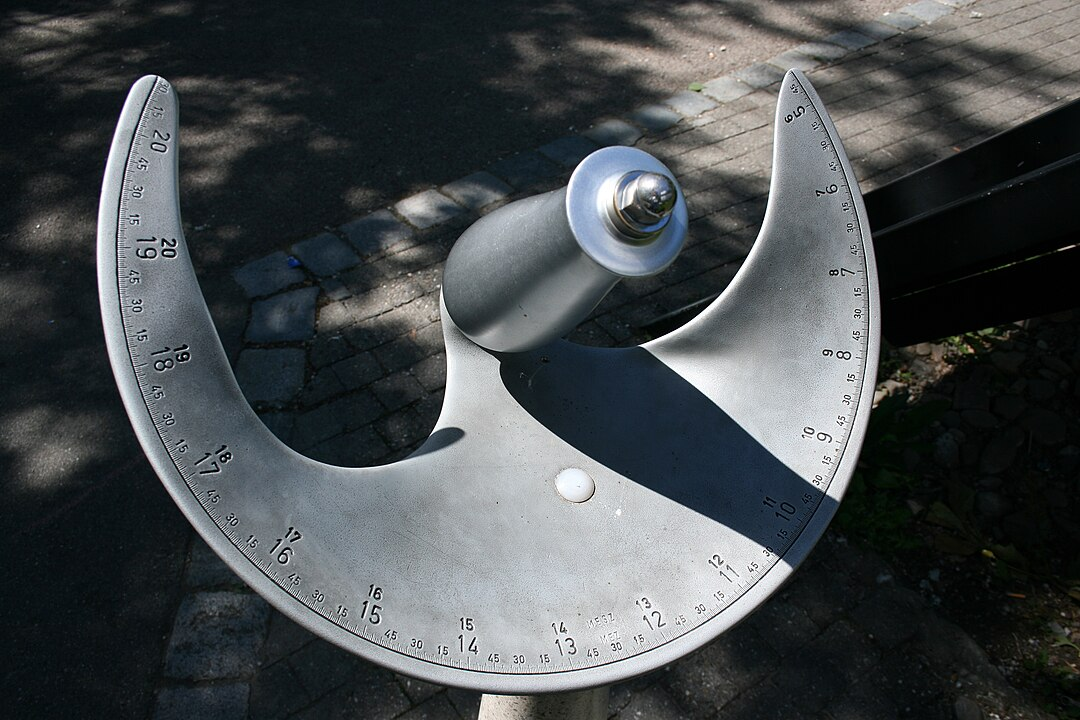
\includegraphics[scale=0.2]{./Bilder/Bernhardt.jpg}
\caption{\label{fig_Bernhardt}%
Sonnenuhr mit Bernhardt'scher Winterwalze. (aus \cite{Wikipedia_Sonnenuhr})}
\end{SCfigure}

Im Verlauf der Zeit verschieben sich die beiden Beitr\"age zur Zeitgleichung gegeneinander. 
W\"ahrend sich der Neigungswinkel zur Ekliptik nur sehr wenig und \"uber einen sehr gro\ss en
Zeitraum von \"uber 40\,000 Jahren ver\"andert, wandert das Perihel im Verlauf von rund 
21\,000 Jahren einmal durch das Jahr. Dadurch ver\"andert sich die Zeitgleichung langsam
und somit auch die Form des Analemmas. Derzeit ist das Analemma leicht asymmetrisch,
weil die Wintersonnenwende und das Perihel nicht auf denselben Tag fallen (das war z.B.\ im
Jahr 1246 der Fall). Au\ss erdem sind die beiden \glqq Hanteln\grqq\ der Acht unterschiedlich 
gro\ss. Wenn das Perihel im Fr\"uhlings- bzw.\ Herbstpunkt steht, sind die beiden Teile
gleich gro\ss.  

\subsection{Der k\"urzeste Tag}

Die Wintersonnenwende entspricht gemeinhin dem k\"urzesten Tag. Derzeit liegt dieses Ereignis
um den 21.\ Dezember.\index{Wintersonnenwende} 
Zu diesem Zeitpunkt befindet sich sie Sonne \"uber dem s\"udlichen
Wendekreis (dem Wendekreis des Steinbocks).\index{Wendekreis des Steinbocks} 
In Freiburg liegen zwischen Sonnenaufgang\index{Freiburg!Sonnenauf-,-untergang}
und Sonnenuntergang an diesem Tag 8 Stunden, 22 Minuten und 13 Sekunden. Doch k\"urzester 
Tag hei\ss t nicht, dass es an diesem Tag am fr\"uhesten dunkel wird oder am sp\"atesten
hell. Der fr\"uheste Sonnenuntergang liegt um den 11.\ Dezember (in Freiburg um 16:35),
der sp\"ateste Sonnenaufgang ist um den 2.\ Januar (in Freiburg gegen 8:18). Alle angegebenen
Uhrzeiten beziehen sich nat\"urlich auf die mittlere Sonnenzeit (genauer MEZ) und nicht die
wahre Sonnenzeit. Der Grund f\"ur den Unterschied ist die Zeitgleichung. 

Eine \"ahnliche Aussage gilt f\"ur die Sommersonnenwende.\index{Sommersonnenwende} 
Der l\"angste Tag mit
16 Stunden 2 Minuten und 47 Sekunden in Freiburg ist der 21.\ Juni. Doch der fr\"uhste Sonnenaufgang
liegt um den 16./17.\ Juni (gegen 5:18), der sp\"ateste Sonnenuntergang um den 25./25.\ Juni (gegen
21:32). Genaue Zeiten f\"ur die Tagesl\"ange, Sonnenauf- und Untergang sowie weitere
interessante Daten f\"ur jeden beliebigen Ort der Erde findet man auf der Webseite \cite{timeanddate}.

\section{Anhang}
\subsection{\"Aquivalenz des zweiten Kepler'schen Gesetzes und der Drehimpulserhaltung}
\label{sec_Zeitgleichung_A}

Sei $\pmb{r}$ der Verbindungsvektor von einem Brennpunkt der Ellipse - dem Brennpunkt, in 
dem sich die Sonne befindet - zu einem Punkt auf der Ellipse (dem Ort eines Planeten)
und $\Delta \pmb{r}$ die in der Zeit $\Delta t$ zur\"uckgelegte Strecke in tangentialer
Richtung. Das zweite Kepler'sche Gesetz\index{Kepler'sches Gesetz!zweites} 
besagt, dass die in dem Zeitraum $\Delta t$ (f\"ur $\Delta t\rightarrow 0$)
\"uberstrichene Fl\"ache $\Delta F$, d.h.
\begin{equation}
                    \Delta F = \frac{1}{2} \pmb{r} \times \Delta \pmb{r} \, ,
\end{equation} 
entlang der Bahnkurve immer gleich ist. Damit ist aber auch der Drehimpuls
\begin{equation}
                    \pmb{L} = m  \pmb{r} \times \frac{{\rm d} \pmb{r}}{{\rm d} t} 
\end{equation} 
konstant.\index{Drehimpulserhaltung}
Das Argument gilt nat\"urlich auch in der umgekehrten Richtung: Aus der
Drehimpulserhaltung folgt das zweite Kepler'sche Gesetz.


\begin{thebibliography}{99}
\bibitem{Wikipedia_Analemma} aus Wikipedia \glqq Analemma\grqq; S.\ Wetzel, CC BY-SA 4.0.
\bibitem{Niermann} Till Niermann - Eigenes Werk, CC BY-SA 3.0, 
                \url{https://commons.wikimedia.org/w/index.php?curid=21792620}
\bibitem{Puzzle} Ravensburger Puzzle; Antique World Map, Hondius.                 
\bibitem{timeanddate} 
   {\small \verb+https://www.timeanddate.com/sun/germany/freiburg+} 
\bibitem{Wikipedia_Sonnenuhr} Wikipedia \glqq Sonnenuhr\grqq; 
           Pr\"azisions-Sonnenuhr mit Winterwalze am Carl Zeiss Planetarium, Stuttgart.
           \url{https://de.wikipedia.org/wiki/Sonnenuhr}   
\bibitem{Wikipedia_Zeitgleichung} Wikipedia \glqq Zeitgleichung\grqq; 
                 \url{https://de.wikipedia.org/wiki/Zeitgleichung} (aufgerufen am 14.5.2023).
\bibitem{Wikipedia_Zeitzone} Wikipedia \glqq Zeitzone\grqq. \url{https://de.wikipedia.org/wiki/Zeitzone}
\end{thebibliography}


\end{document}


%\documentclass[german,10pt]{book}      
\usepackage{makeidx}
\usepackage{babel}            % Sprachunterstuetzung
\usepackage{amsmath}          % AMS "Grundpaket"
\usepackage{amssymb,amsfonts,amsthm,amscd} 
\usepackage{mathrsfs}
\usepackage{rotating}
\usepackage{sidecap}
\usepackage{graphicx}
\usepackage{color}
\usepackage{fancybox}
\usepackage{tikz}
\usetikzlibrary{arrows,snakes,backgrounds}
\usepackage{hyperref}
\hypersetup{colorlinks=true,
                    linkcolor=blue,
                    filecolor=magenta,
                    urlcolor=cyan,
                    pdftitle={Overleaf Example},
                    pdfpagemode=FullScreen,}
%\newcommand{\hyperref}[1]{\ref{#1}}
%
\definecolor{Gray}{gray}{0.80}
\DeclareMathSymbol{,}{\mathord}{letters}{"3B}
%
\newcounter{num}
\renewcommand{\thenum}{\arabic{num}}
\newenvironment{anmerkungen}
   {\begin{list}{(\thenum)}{%
   \usecounter{num}%
   \leftmargin0pt
   \itemindent5pt
   \topsep0pt
   \labelwidth0pt}%
   }{\end{list}}
%
\renewcommand{\arraystretch}{1.15}                % in Formeln und Tabellen   
\renewcommand{\baselinestretch}{1.15}                 % 1.15 facher
                                                      % Zeilenabst.
\newcommand{\Anmerkung}[1]{{\begin{footnotesize}#1 \end{footnotesize}}\\[0.2cm]}
\newcommand{\comment}[1]{}
\setlength{\parindent}{0em}           % Nicht einruecken am Anfang der Zeile 

\setlength{\textwidth}{15.4cm}
\setlength{\textheight}{23.0cm}
\setlength{\oddsidemargin}{1.0mm} 
\setlength{\evensidemargin}{-6.5mm}
\setlength{\topmargin}{-10mm} 
\setlength{\headheight}{0mm}
\newcommand{\identity}{{\bf 1}}
%
\newcommand{\vs}{\vspace{0.3cm}}
\newcommand{\noi}{\noindent}
\newcommand{\leer}{}

\newcommand{\engl}[1]{[\textit{#1}]}
\parindent 1.2cm
\sloppy

         \begin{document}  \setcounter{chapter}{3}


\chapter{Zeitsysteme}
% Kap 4
\label{chap_Zeitsysteme}

\info{Thomas Filk}{28.03.2024}%
Seit 1967 ist die Sekunde\index{Sekunde} 
durch die Frequenz $\Delta \nu_{\rm Cs}$ des Hyperfeinstruktur\"ubergangs\index{Hyperfeinstruktur\"ubergang}
in 133-C\"asium im Grundzustand definiert. Es gilt:
\begin{equation}
               1\,{\rm s}  =  9\,192\,631\,770 \, T = 9\,192\,631\,770 \, \frac{1}{\Delta \nu_{\rm Cs}} \, .
\end{equation}  
$T$ ist die Periodenl\"ange einer Schwingung zu diesem \"Ubergang.
Die Definition der Sekunde \"uber den Hyperfeinstruktur\"ubergang in 133-C\"asium l\"oste 1967 die 
Ephemeridensekunde ab, die \"uber die Position der Erde relativ zur Sonne definiert 
war.\index{Zeitsysteme|(} 

Man k\"onnte meinen, dass mit der Definition der SI-Sekunde und der Konstruktion von
Uhren, die diese Sekunde genau genug messen k\"onnen, das Problem der Zeitmessung
gel\"ost sei. Im Detail ergeben sich jedoch Probleme, die zu verschiedenen
Zeitsystemen gef\"uhrt haben. Zum einen muss man zwischen theoretischen Zeitsystemen,
die auf idealen Uhren basieren, und den Realisierungen solcher Zeitsysteme durch
tats\"achlich existierende und mit Fehlern behaftete Uhren unterscheiden. In diesem Zusammenhang
ist zu definieren, wie man aus den fehlerbehafteten Werten realer Messinstrumente eine Zeitskala
definiert kann. Au\ss erdem muss
man einen Referenzpunkt w\"ahlen, da nach der speziellen und allgemeinen Relativit\"atstheorie
Uhren an verschiedenen Orten (im Gravitationsfeld) oder in verschiedenen Bewegungszust\"anden
unterschiedliche Zeitsysteme definieren. Und schlie\ss lich m\"ochte man nat\"urlich, dass die
Zeitsysteme trotz ihrer derzeitigen Definition \"uber atomare Eigenschaften noch etwas mit dem 
Tag-und-Nacht-Rhythmus der Erde zu tun haben.

Auch heute noch sind verschiedene Zeitsysteme in Gebrauch. Die folgende Liste bzw.\ Behandlung
dieser Zeitsysteme kann daher nur einen groben \"Uberblick geben. 

\section{Das Julianische Datum}

Die Julianische Tagesz\"ahlung (englisch \textit{Julian day}) z\"ahlt, unabh\"angig von einem 
speziellen Kalender oder der Definition eines Jahres,\index{Julianische Tagesz\"ahlung}
die Tage seit einem Anfangsdatum, das als der 1.\ Januar des Jahres 4713 v.\,Chr.\ nach dem
zur\"uckextrapolierten Julianischen Kalender gew\"ahlt wird. Genauer beginnt diese Z\"ahlung mittags
um 12 Uhr (Sonnenh\"ochstand am heutigen Nullmeridian durch Greenwich). W\"ahlt man nicht den
zur\"uckgerechneten Julianischen Kalender sondern den zur\"uckgerechneten Gregorianischen
Kalender, so beginnt diese Zeitrechnung mit dem 24.\ November des Jahres 4714 v.\,Chr. Und da es
weder im Julianischen noch im Gregorianischen Kalender das Jahr 0 gibt, entspricht das Jahr 4713 dem
Jahr $-$4712 im astronomischen Kalender, der das Jahr 0 hinzunimmt. 

Die Wahl dieses Datums hat historische Gr\"unde. Zun\"achst werden hier drei Zyklen zu einer
Epoche zusammengefasst: Der Menton-Zyklus\index{Menton-Zyklus} 
oder Mondzyklus von 19 Jahren, der Sonnenzyklus\index{Sonnenzyklus}
von 28 Jahren\footnote{Im Julianischen Kalender haben 4 Jahre - die Periode dieser Kalenderz\"ahlung - 
eine Dauer von 1461 Tagen, dabei verschieben
sich die Wochentage um 5 Tage - der Rest bei einer Teilung von 1461 durch 7. 
Alle $4\times 7=28$ Jahre fallen also die Wochentage wieder auf dasselbe Datum. Im
Gregorianischen Kalender entspricht eine Periode 400 Jahren mit 146\,097 Tagen. Dies ist glatt durch 7 teilbar,
d.h.\ alle 400 Jahre fallen im Gregorianischen Kalender dieselben Daten wieder auf dieselben Wochentage.}
und der sogenannte Indiktionszyklus\index{Indiktionszyklus} 
von 15 Jahren (ein Zyklus, der im Altertum und Mittelalter
oft verwendet wurde und urspr\"unglich mit Neuberechnungen der Steuern einherging). 
Das Produkt dieser drei Zyklenl\"angen sind
7980 Jahre; dies bezeichnet man als eine Epoche. Das Jahr 4713 v.Chr.\ wurde im Mittelalter errechnet
als ein Jahr, in dem alle drei genannten Zyklen nach damaliger Rechnung begannen. Es hat den Vorteil, dass
es vor jeder historischen Datierung liegt, d.h.\ es gibt keine datierten historischen Ereignisse vor diesem
Jahr (au\ss er astronomische Ereignisse, die man heute zur\"uckrechnen kann). 

Dem Julianische Tag, der am 1.\ Januar 2000 mittags 12 Uhr (Universal time im Gregorianischen Kalender) begann, 
entspricht nach der Julianischen Tagesz\"ahlung  der Tag 2\,451\,545. Soviel Tage sind seit dem 1.\ Januar 4713 v.\,Chr.\
nach dem zur\"uckgerechneten Julianischen Kalender vergangen. Diese Z\"ahlung ist so einfach, dass
sie nicht nur in der Astronomie gerne verwendet wird, sondern auch in abgewandelter
Form in vielen Computersystemen. 

Will man neben dem Tag auch die Uhrzeit ber\"ucksichtigen, werden Nachkommastellen angegeben.
Der Tag hat 86\,400 Sekunden, sodass der 1.\ Januar 2000, 22 Uhr 25 Minuten und 10 Sekunden dem
Julianischen Datum 2\,451\,545,43414 entspricht. Sowohl die Julianische Tagesz\"ahlung (im Englischen
\textit{Julian Day}) als auch das\index{Julianisches Datum}  
Julianische Datum (\textit{Julian Date}) werden mit JD abgek\"urzt. 
Man beachte, dass diese Tagesz\"ahlung abgesehen von der Angabe des Anfangsdatums
nicht davon abh\"angt, ob ansonsten der Julianische oder Gregorianische Kalender (oder welcher andere 
Kalender auch immer) verwendet wird. 

Eine h\"aufig verwendete Abwandlung ist das sogenannte\index{Julianisches Datum!Modfiziertes} 
Modifizierte Julianische Datum, abgek\"urzt mit
MJD. Dies wird beispielsweise auch von dem BIPM (Bureau International des Poids et Mesures) in seinen
\textit{Circular T},\index{Circular T}\index{BIPM, Bureau International des Poids et Mesures} 
den monatlichen Berichten zur Bestimmung der Internationalen Atomzeit TAI,
verwendet. Das MJD unterscheidet sich vom JD in zwei Punkten:
\begin{enumerate}
\item
Der Tagesanfang wird auf 0 Uhr Mitternacht (statt auf 12 Uhr mittags) gelegt.
\item  
Der Beginn ist 0 Uhr, 17.\ November 1858. Das bedeutet, vom Julianischen Tag werden 2\,400\,000,5 Tage
abgezogen: ${\rm MJD=JD}-2\,400\,000,5$.       
\end{enumerate}
Damit hat der 1.\ Januar 2000, 12 Uhr mittags, den Wert: ${\rm MJD}= 51\,544,5$.  

\section{Die Ephemeridenzeit - ET}

Die\index{Ephemeridenzeit} 
Sekunde als der 1/86\,400-ste Teil eines Tages ist erst seit dem Mittelalter in Gebrauch
und bis 1956 war die Sekunde als der 1/86\,400-ste Teil eines mittleren Sonnentages definiert. 
Man wusste zu diesem Zeitpunkt allerdings schon, dass auch der mittlere Sonnentag nicht wirklich
vollkommen gleichm\"a\ss ig verl\"auft bzw.\ dass der mittlere Sonnentag davon abh\"angt, \"uber
welchen Zeitraum genau gemittelt wird. Daher verwendete man schon seit l\"angerem die Stellung
der Erde relativ zur Sonne zur Definition einer Sekunde. So war in der Zeit zwischen 1956 und 1968
die Sekunde definiert als der 1/31\,556\,925,9747-ste Teil des tropischen Jahres 1900 
(genauer: des theoretisch hochgerechneten tropischen
Jahres 1900, bestimmt aus den Bahndaten der Erde zum Zeitpunkt 31.12.1899, mittags 12 Uhr).
Diese Definition der Sekunde bezeichnet man auch als die 
Ephemeridensekunde.\index{Ephemeridensekunde}

Schon in babylonischer Zeit (um 1000 v.\,Chr.) gab es Tabellen zu den Positionen von Sonne, Mond und
Planeten, und der sogenannte\index{Almagest (Ptolem\"aus)} 
Almagest von Ptolem\"aus mit seinen genauen Beschreibungen der
Planetenbahnen gilt als H\"ohepunkt antiker Astronomie. Im Mittelalter wurden weitere 
Tabellen\index{Ephemeridentabellen} 
erstellt (bekannt sind die Toledaner Tafeln aus dem 12.\ Jahrhundert, die Alfonsinischen Tafeln 
aus dem 13.\ Jahrhundert, die Ephemeridentafeln von Regiomontanus von 1474, oder 
auch die Rudolfinischen Tafeln von 1627 von Johannes Kepler).  
  
Seit dem Mittelalter gab es Tabellen, in denen die Position der Sonne, des Mondes und der Planeten
relativ zu einem Koordinatensystem (meist durch Angabe der Rektazension und Deklination) 
und/oder relativ zueinander mit Daten und Tageszeiten korreliert wurden. 

\section{TT, TCG und TCB}
 
TT (\textit{Terrestial Time} oder \textit{Temps terrestre}), TCG (\textit{Geocentric Coordinated Time} oder
\textit{Temps-coordonn\'{e}e geocentrique}) und TCB (\textit{Barycentric Coordinate Time} oder
\textit{Temps-coordonn\'{e}e barycentrique}) sind idealisierte Zeitsysteme, manchmal spricht man auch von
Platonischen Zeitsystemen,\index{Zeitsystem!Platonisches} 
die auf idealen Uhren unabh\"angig von konkreten Realisierungen beruhen.
Sie dienen meist der theoretischen Beschreibung von Objekten in unserem Sonnensystem. 

TCB (baryzentrische koordinierte Zeit)\index{TCB, baryzentrisch koordinierte Zeit} 
ist die Zeit einer idealen, die SI-Sekunde anzeigenden Uhr, 
die sich in einem idealisierten hypothetischen 
System befindet, das sich parallel zum Schwerpunkt (dem Baryzentrum) des Sonnensystems bewegt,
also dieselben Bewegungen wie dieser Schwerpunkt ausf\"uhrt, aber keinem Gravitationspotenzial
unterliegt. Es wird typischerweise f\"ur die Beschreibung von Bahnkurven von Planeten oder Kometen
verwendet sowie von Raketen oder Satelliten, die den gravitativen Einfluss der Erde verlassen. 
Entsprechend ist\index{TCG, geozentrisch koordinierte Zeit} 
TCG (geozentrische koordinierte Zeit) die Zeit einer idealen, die SI-Sekunde anzeigenden 
Uhr, die sich in einem idealisierten System befindet, das sich parallel zum Schwerpunkt des Erdmittelpunkts 
bewegt, aber keinem Gravitationspotenzial unterliegt. Sie dient zur Beschreibung von Bahnkurven im 
gravitativen Einfluss der Erde, beispielsweise den Bahnkurven von Satelliten, dem Mond oder Raketen. 

TT (terrestrische Zeit)\index{TT, terrestrische Zeit} 
ist die Zeit einer idealen Uhr, die sich auf der Oberfl\"ache der Erde befindet. Hierbei ist die Oberfl\"ache
definiert durch die gravitative \"Aquipotentialfl\"ache (also konstantes Gravitationspotenzial) zur mittleren 
Meeresh\"ohe, wobei der Effekt der Erddrehung (Potenzial zur Fliehkraft) 
einbezogen wird, nicht jedoch der Einfluss von Str\"omungen oder Gezeiten. Diese Fl\"ache bezeichnet man
auch als das Geoid der Erde. Da die mittlere Meeresh\"ohe\index{Meeresh\"ohe, mittlere}
(z.B.\ im Zusammenhang mit dem Klimawandel) keine Konstante ist, hat man f\"ur das Potenzial
den Wert $U/c^2=6,969\,290\,134\cdot 10^{-10}$ definiert (der Quotient aus einem Potenzial
und $c^2$ ist eine dimensionslose Konstante), was bei einer homogenen Kugel von der Masse der Erde
einem Radius von etwas \"uber 6\,360\,km entspricht. 

TT und TCG unterscheiden sich also um einen multiplikativen Faktor $( 1 - U/c^2)$, um den TT langsamer
ist als TCG. Au\ss erdem wurde definiert, dass die beiden Zeiten am 1.\ Januar 1977, um 0 Uhr 32,184 Sekunden,
gleich waren. Die seltsame Sekundenzahl ergibt sich daraus, dass TT m\"oglichst exakt an die vorher
gebr\"auchliche Ephemeridenzeit angepasst werden sollte. Au\ss erdem entspricht diese Zeit exakt 0 Uhr nach 
der Internationalen Atomzeit TAI (siehe n\"achsten Abschnitt). Fr\"uher verwendete man f\"ur die terrestrische
Zeit TT die Bezeichnung TDT\index{TDT, terrestrial dynamical time} 
(terrestrial dynamical time); diese Bezeichnung findet man gelegentlich immer noch.  

\section{Die Internationale Atomzeit - TAI}

Die Internationale Atomzeit TAI\index{TAI, internationale Atomzeit} 
(\textit{Temps atomique international}) ist eine Realisierung von TT. Hierbei
handelt es sich um eine Zeit, die an existierenden Uhren abgelesen wird. Da eine einzelne Uhr immer
ungenau ist und auch mal St\"orungen haben kann, handelt es sich bei TAI um einen gewichteten
Mittelwert von derzeit \"uber 400 hoch pr\"azisen Uhren an \"uber 80 Orten. In der Physikalisch Technischen
Bundesanstalt (PTB)\index{PTB, Physikalisch Technische Bundesanstalt} 
in Braunschweig stehen zwei solche Atomuhren - genannt CSF1 und CSF2, hierbei handelt
es sich um C\"asium Fountain Clocks -, die zur
TAI beitragen. In regelm\"assigen Abst\"anden \"ubermitteln diese Uhren ihre Zeiten an das
BIPM. Dort werden die Daten um verschiedene Faktoren korrigiert (dazu z\"ahlen Laufzeiten der \"Ubertragung
sowie relativistische Korrekturen aufgrund der H\"ohenunterschiede der verschiedenen Uhren), die
Uhren mit den gr\"o\ss ten Abweichungen werden nicht ber\"ucksichtigt und von rund 300 Uhren wird
ein gewichtetes Mittel gebildet. Die Gewichtung der einzelnen Uhren richtet sich nach ihrem gesch\"atzten 
Fehler (der sich aus einer Theorie ihrer Funktionsweise bestimmt) sowie Ungenauigkeiten oder
Schwankungen in der Vergangenheit. Einmal im Monat wird im
\textit{BIPM Circular T} ver\"offentlicht, um wie viel die einzelnen Uhren von dem berechneten Mittelwert
zu bestimmten Zeitpunkten (die dann rund einen Monat zur\"uckliegen) abwichen. 

TAI versucht also eine m\"oglichst genaue Realisation einer idealen, die SI-Sekunde anzeigenden Uhr
zu sein, die sich auf der Oberfl\"ache des Geoids befindet. 
Insofern ist sie eine Realisation von TT, bis auf die oben erw\"ahnten 32,184 Sekunden, um die
sich die beiden Zeiten am 1.\ Januar 1977, 0 Uhr (TAI-Zeit), unterschieden. TT sollte dabei an die Ephemeridenzeit
angepasst werden, an die TAI schon 1958 angepasst worden war. Die 32,184 Sekunden Unterschied
erkl\"aren sich also daher, dass zwischen diesen beiden Zeitpunkten (1958 und 1977) schon ein
solcher Unterschied zwischen der Atomzeit und der Ephemeridenzeit bestand. 

\section{Universal Times - UT0, UT1, UT2}

Die\index{UT, Universal Times} 
Universal Times beziehen sich direkt auf die Lage der Erde und sind somit eine Fortf\"uhrung
der Ephemeridenzeit. Die Universal Time ist definiert \"uber den Winkel, den der Nullmeridian auf der
Erde relativ zu einem ausgezeichneten Punkt auf dem Himmels\"aquator (der Projektion des Erd\"aquators
vom Mittelpunkt der Erde aus auf die Himmelskugel) hat. Dieser Punkt auf dem Himmels\"aquator
ist heute definiert \"uber ein Referenzsystem am Himmel, das \"uber die Lage von festen Punkten am
Himmel - meist Quasare, die auch im Radiowellenbereich nachweisbar sind, sodass eine VLBI (Very Long
Baseline Interferometry) eine sehr genaue Richtungsbestimmung auch am Tag erm\"oglicht - definiert ist. Dieses
Referenzsystem bezeichnet\index{ICRF, International Celestial Reference Frame} 
man auch als ICRF (\textit{International Celestial Reference Frame}).   

Die Ephemeridenzeit bezog sich auf einen gemittelten Tag, wie er durch das (vom 31.12.1899, 12 Uhr, hochgerechnete) Jahr 1900 definiert war.\index{GMT, Greenwich Mean Time} 
Diese Zeit nannte man auch GMT (\textit{Greenwich Mean Time}). Sie entspricht genau
dem, was man sp\"ater UT0 nannte: Eine Zeitbestimmung \"uber einen gemittelten Sonnentag, also die Zeit
eines realen Sonnentags, die durch die Zeitgleichung - also die Einfl\"usse der elliptische Bahn der Erde sowie ihrer Neigung
gegen\"uber der Ekliptik - korrigiert wird und somit zur Zeit eines mittleren Sonnentags geh\"ort. 
Der Winkel ERA (\textit{Earth Rotation Angle})\index{ERA, Earth Rotation Angle} 
des Nullmeridians relativ zu dem Referenzsystem am Himmel  
ist bis auf eine Konstante direkt proportional zur UT. Die Proportionalit\"atskonstante ber\"ucksichtigt, dass es sich
hierbei um eine Messung der Erdrotation relativ zu einem Himmelssystem (siderischen Referenzsystem)
handelt, und diese Zeit korrigiert werden muss, um einen Sonnentag zu erhalten. Dementsprechend entspricht
dieser Proportionalit\"atsfaktor ziemlich genau dem Faktor $(1+1/365,25)$, um den der siderische Tag im 
Vergleich zum Sonnentag korrigiert werden muss. Genauer lautet die Beziehung:
\begin{equation}
      {\rm ERA} = 2\pi (0,7790572732640 + 1,00273781191135448 \cdot T_{\rm u}) \, {\rm rad}  \, ,
\end{equation}
wobei $T_{\rm u} = ({\rm JD(UT1)} - 2\,451\,545,0)$ ist, und ${\rm JD(UT1)}$ dem Julianischen Datum
nach der UT1-Uhrzeit entspricht. ERA ist die gemessene Variable (ein Winkel) und JD(UT1) - ein Datum
mit einem Zeitpunkt - wird daraus berechnet. ERA, also der gemessene Winkel, wird dabei um zwei
Faktoren korrigiert: (1) die Zeitgleichung, die den Unterschied zwischen mittlerem und wahrem 
Sonnentag angibt, und (2) Schwankungen in der Drehachse der Erde (sogenannte Polarbewegungen), durch die
der L\"angengrad, beispielsweise eines Observatoriums, nicht eindeutig bestimmt ist. Weitere jahreszeitliche
Schwankungen, die beispielsweise in dem Zeitsystem UT2 ber\"ucksichtigt werden, werden f\"ur UT1 nicht
ber\"ucksichtigt.       

\section{Universal Coordinated Time - UTC}

Wir haben nun zwei realisierte Zeitsysteme (d.h., Zeitsysteme, die durch Messungen an realen physikalischen Systemen bestimmt werden): 
Die TAI, die \"uber Atomuhren bestimmt wird, die m\"oglichst nahe an der SI-Sekunde
arbeiten, und UT1, die \"uber die Lage der Erde relativ zur Sonne bestimmt wird. UT1 hat den Vorteil, dass 12 Uhr
mittags mit unserer Vorstellung von \glqq Sonnenh\"ochststand\grqq\ zusammenf\"allt, wohingegen TAI auf einer
m\"oglichst genauen und gleichm\"a\ss igen Realisierung einer Sekunde beruht. Damit entsteht das Problem:
An welches Zeitsystem sollen wir uns halten, wenn diese beiden Zeitsysteme auseinanderlaufen. UT1 hat den Vorteil,
unseren Vorstellung von Tag und Nacht zu entsprechen, TAI hat den Vorteil, dass die Sekunden immer gleich
lang sind. 

Um ein Auseinanderlaufen der beiden Zeitsysteme auszugleichen, hat man sich (nach anf\"anglichen Problemen bei
der Namensgebung wie auch bei der genauen Definition) 1972 auf das Zeitsystem 
der UTC\index{UTC, Universal Coordinated Time}
(\textit{Universal Coordinated Time}) geeinigt. UCT verl\"auft parallel zu TAI, d.h., UTC richtet sich bez\"uglich
der genauen Zeitangabe nach der besten Realisierung der SI-Sekunde auf der Erdoberfl\"ache, und das ist
die TAI. Bevor allerdings UT1 und TAI um 0,9 Sekunden auseinanderlaufen (weil die Erddrehung gewissen
Schwankungen unterworfen ist), wird f\"ur UTC eine\index{Schaltsekunde} 
Schaltsekunde entweder eingef\"ugt oder weggelassen.
In der Vergangenheit wurden nur Schaltsekunden eingef\"ugt, da die Erdrotation etwas langsamer ist als
die TAI-Zeit. Als UTC im Jahre 1972 eingef\"uhrt wurde bestand schon ein Unterschied von 10 Sekunden
zwischen UT1 und TAI, sodass damals definiert wurde UTC = TAI - 10\,s. Seitdem wurden insgesamt 27
weitere Schaltsekunden eingef\"ugt, die letzte am 31.\ Dezember 2016. S\"amtliche Schaltsekunden wurden
in der Vergangenheit entweder am 31.\ Juni oder am 31.\ Dezember eingef\"ugt. In den letzten Jahren hat
die Geschwindigkeit der Eigendrehung der Erde wieder etwas zugenommen, sodass nicht ausgeschlossen
wird, dass in der nahen Zukunft zum ersten Mal in der Geschichte der UTC eine Sekunde \glqq herausgenommen\grqq\ wird. 

Das Einf\"ugen von Schaltsekunden f\"uhrte dazu, dass im Zeitsystem der UTC gelegentlich eine Minute
61 Sekunden hat. Statt nach der 59.-sten Sekunde die 0.te Sekunde folgen zu lassen, z\"ahlt man 
eine 60.ste Sekunde hinzu und beginnt dann den neuen Monat mit der Sekunde 0. Da in der Vergangenheit
noch nie eine Schaltsekunde entfernt wurde, gibt es gewisse Bedenken, ob alle Computersysteme mit einem
solchen Schritt zurecht kommen. Da auch beim Einf\"ugen von Schaltsekunden in der Vergangenheit immer
wieder Probleme mit verschiedenen digitalen Systemen auftraten, wurde in j\"ungerer Zeit \"uberlegt, die
Definition von UTC nochmals zu \"andern. Es wird angestrebt, bis 2035 eine neue Definition zu finden, bei
der nur alle paar Jahrhunderte eine Korrektur notwendig wird \cite{BIPM2022}. Beispielsweise k\"onnte man die Differenz
zwischen UT1 und TAI auf mehrere Minuten anwachsen lassen, bevor Korrekturen vorgenommen werden.
Rein subjektiv werden wir als Menschen die langsame Verschiebung der Mittagsstunde ohnehin erst
bemerken, wenn sich die Differenz auf die Gr\"o\ss enordnung einer Stunde summiert hat. 

Die UTC ist die Zeit, die wir beispielsweise \"uber Funkuhren, das Radio oder Fernsehen empfangen.
Diese Zeit ist bis auf 0,9 Sekunden an die Orientierung der Erde relativ zum Referenzsystem des Himmels
angepasst, l\"auft parallel zur Atomzeit TAI, d.h.\ ist sehr regelm\"a\ss ig, hat aber den Nachteil, 
dass eine Minute gelegentlich eine Sekunde mehr oder weniger hat. Wegen der Unregelm\"a\ss igkeit
der Erddrehung k\"onnen Schaltsekunden nicht langfristig vorhergesagt werden, sondern erst in einem
Zeitraum von einem halben Jahr. 

\section{Lokalzeit - Local Time}

Die Lokalzeit\index{Lokalzeit} 
ist die Zeit, die von Radio- oder Fernsehstationen, Funkuhren bzw.\ \"offentlichen Uhren
an einem Ort angezeigt wird. Sie richtet sich nach der UTC, unterliegt also unter anderem der 
Einf\"ugung oder L\"oschung von Schaltsekunden, unterscheidet sich von der UTC aber in zweierlei
Hinsicht:
\begin{enumerate}
\item
Sie\index{Zeitzone} 
ber\"ucksichtigt die lokale Zeitzone: UTC ist die Fortsetzung der GMT (Greenwich Mean Time) und
richtet sich nach dem Nullmeridian durch Greenwich, d.h.\ nach dem L\"angengrad, wo im Jahresmittel
mittags um 12 Uhr die Sonne ihren H\"ochststand hat. Damit man an nahezu allen Orten um die Mittagszeit
den Sonnenh\"ochststand hat, wurde die Erde in Zeitzonen eingeteilt, die einseits von L\"angengraden,
andererseits aber auch von L\"andergrenzen berandet sind. Die meisten Zeitzonen unterscheiden sich
von der Zeitzone von Greenwich um ein Vielfaches einer vollen Stunde. Alle 15 L\"angengrade beginnt also rein rechnerisch
eine neue Zeitzone, wobei die meisten L\"ander (Ausnahmen sind die USA, Kanada, Russland und
Australien) nur eine Zeitzone haben, was z.B.\ f\"ur China bedeutet, dass es sich rechnerisch \"uber 
fast vier Zeitzonen erstreckt aber im gesamten Land dieselbe Zeitzone gilt. 
Es gibt aber auch einige L\"ander mit halbst\"undiger Zeitverschiebung (Iran $+3\frac{1}{2}$, Afghanistan $+4\frac{1}{2}$,
Indien $+5\frac{1}{2}$, Burma $+6\frac{1}{2}$, Zentralaustralien $+9\frac{1}{2}$) sowie   
viertelst\"undiger Zeitverschiebung (Nepal $+5\frac{3}{4}$, kleine Teile von Australien $+8\frac{3}{4}$
sowie die Chatham Islands $+10\frac{3}{4}$). 

Zentraleuropa (mit Ausnahme von Portugal und\index{MEZ, mitteleurop\"aische Zeit}
den Inselgruppen Kanaren, Madeira, Island und Azoren) verwenden die Mitteleurop\"aische Zeit (MEZ), die
sich von der UTC um +1 Stunde unterscheidet, d.h., wenn es in Greenwich 12 Uhr mittags ist, ist es in
Mitteleuropa bereits 1 Uhr mittags. 
\item
In den Sommermonaten\index{Sommerzeit} 
wechseln viele L\"ander auf die Sommerzeit. Dazu verschiebt man die Zeitzone um eine
weitere Stunde nach Osten, d.h., relativ zum Sonnenstand ist es eine Stunde sp\"ater. Damit verbunden ist etwas
l\"angere Dunkelheit am Morgen und etwas l\"angere Helligkeit am Abend. In diesem Fall spricht man in
Mitteleuropa von der\index{MESZ, Mitteleurop\"aische Sommerzeit} 
MESZ - Mitteleurop\"asische Sommerzeit, die sich von der UTC um +2 Stunden unterscheidet.      
\end{enumerate}
Ungef\"ahr entlang des 180-sten L\"angengrads (im Pazifik, durch die Fiji-Inseln) verl\"auft die Internationale Datumsgrenze.\index{Datumsgrenze}
\"Uberquert man diese Grenze von West nach Ost, muss man das Datum um einen Tag zur\"uckstellen, \"uberquert
man sie von Ost nach West stellt man das Datum um einen Tag vor. 

\section{GPS Time}

Abschlie\ss end soll noch kurz auf die GPS-Zeit\index{GPS-Zeit}\index{GPS, Global Positioning System} 
des Global Positioning Systems (GPS) eingegangen werden. 
Das GPS besteht unter anderem aus 24 aktiven Satelliten (es befinden sich derzeit - Dezember 2022 - 32
Satelliten im Orbit, davon sind 31 einsatzbereit, sieben der Satelliten dienen als Backup), die st\"andig ein
Signal aussenden, das die genaue Zeit sowie den genauen Ort dieser Satelliten angibt. Mindestens vier dieser
Satelliten befinden sich jederzeit in \glqq Sichtlinie\grqq\ von jedem beliebigen Punkt der Erde aus. Aus den
Signalen kann ein geeigneter Empf\"anger seine genaue Position sowie die genaue Zeit bestimmen. 

Die vom GPS-System verwendete GPS-Zeit richtet sich im Wesentlichen nach der TAI, d.h.\ es wird die
auf das Geoid der Erde bezogene Eigenzeit verwendet, ohne Einschub oder Wegnahme von Schaltsekunden. 
Das bedeutet unter anderem, dass die Uhren in den GPS-Satelliten \glqq falsch gehen\grqq: Es handelt sich
nicht um SI-Uhren, die die Eigenzeit in dem Satelliten messen, sondern diese Eigenzeiten werden um die
relativistischen Effekte aufgrund der Bewegung des Satelliten sowie des Gravitationsfelds der Erde
korrigiert, sodass diese Uhren die Zeit angeben, die an einem ruhenden Ort auf dem Geoid der Erde
gilt. Damit stimmen diese Uhren in ihrem Zeittakt mit der Atomzeit TAI \"uberein. 

Als Startpunkt der GPS-Zeit wurde 0 Uhr am 6.\ Januar 1980 festgelegt. Zu diesem Zeitpunkt unterschieden
sich UTC und TAI bereits um 19 Schaltsekunden. Da die GPS-Zeit zu diesem Zeitpunkt an die UTC angepasst
wurde, unterscheiden sich GPS-Zeit und TAI also dauerhaft um 19 Sekunden: GPS = TAI - 19\,s. Derzeit (Dezember
2022) unterscheiden sich UTC und GPS-Zeit um 18 Sekunden; diese 18 Sekunden wurden seit dem 6.\ Januar
1980 bei der UTC als Schaltsekunden eingef\"ugt. Damit geht UTC relativ zur GPS-Zeit um 18 Sekunden nach,
d.h.\ es gilt: GPS = UTC + 18\,s. Diese Zeitdifferenz \"andert sich aber, falls bei der UTC Schaltsekunden eingef\"ugt
oder weggelassen werden.   

Die Z\"ahlung bei der GPS-Zeit verwendet mehrere Einheiten: Epochen, Wochen, Tage und Sekunden.
\begin{enumerate}
\item
Eine Epoche\index{Epoche} 
besteht aus 1024 Wochen. Die Wochenzahl wird als 10-Bit Zeichenfolge \"ubertragen. 
Der Woche 1023 folgt die Woche 0. Dies bezeichnet man auch als Rollover.\index{Rollover} 
Eine Epoche dauert somit
7168 Tage oder etwas \"uber 19,6 Jahre. Da diese Rollover (bisher fanden
zwei solche Rollover statt - in der Nacht vom 21.\ auf den 22.\ August 1999 und in der Nacht vom 
6.\ auf den 7.\ April 2019) zu Problemen bei manchen Anwendern gef\"uhrt haben, will
man in naher Zukunft die Zeichenfolge f\"ur die Wochen auf 13 Bit erweitern, sodass nur ungef\"ahr alle 157 Jahre
ein solcher Rollover stattfindet. Derzeit (am 11.\ Dezember 2022) befinden wir uns in der GPS-Woche 2240 (dies ist
die Anzahl der Wochen, die seit dem 6.\ Januar 1980 vergangen sind), also in der 192.\ Woche der Epoche 2.
\item
Die Wochen\index{Woche} 
werden mit Beginn vom 6.\ Januar 1980 gez\"ahlt. Da es jedoch derzeit noch wegen der 10-Bit-Folge
f\"ur die Angabe der Wochen zu Rollover kommt, gibt die GPS-Zeit nur die Wochenzahl der laufenden Epoche
wieder (am 11.\ Dezember 2022 war das die Woche 192). 
\item
F\"ur jede Woche wird der Tag angegeben, also ein Wert zwischen 0 und 6. Die neue Woche beginnt
mit dem Sonntag, dem Tag 0. 
\item
F\"ur jeden Tag werden die Sekunden angegeben. Der Tag beginnt um Mitternacht 0 Uhr.  
\end{enumerate}
Damit besteht eine volle Angabe der GPS-Zeit aus: Wochenzahl (gesamt), Epoche + Woche innerhalb der
Epoche (ein Wert zwischen 0 und 1023), Tag (ein Wert zwischen 0 und 6) und Sekunden an diesem Tag
(ein Wert zwischen 0 und 86399). Die Gesamtzahl der Wochen bzw.\ die Epoche wird allerdings nicht im GPS-Signal kodiert. 
Der Empf\"anger bzw.\ Anwender muss also wissen, in welcher Epoche man sich befindet. 

\section{Kuriosit\"aten}

\subsection{Die Datumsgrenze}

Es wurde oben erw\"ahnt,\index{Datumsgrenze} 
dass man bei der \"Uberquerung der Datumsgrenze von West nach Ost das Datum
um einen Tag zur\"uckstellen muss (also 24 Stunden subtrahieren muss), bei der \"Uberquerung von Ost nach West
muss das Datum entsprechend um einen Tag vorgestellt werden. Als Scherzfrage f\"ur Kinder in den unteren Klassen
bietet sich nun folgendes Gedankenexperiment an: Angenommen, man k\"onnte mit einem sehr schnellen Flugzeug
immer von West nach Ost um die Erde reisen und dabei die Datumsgrenze in kurzer Zeit mehrfach von West nach
Ost \"uberqueren, dann w\"urde man jedesmal das Datum um einen Tag zur\"ucksetzen. Kann man auf diese Weise
in die Vergangenheit reisen, also ist man beispielsweise nach f\"unfmaliger \"Uberquerung der Datumsgrenze um
f\"unf Tage zur\"uckgereist? Eine \"ahnliche Frage kann man nat\"urlich auch bez\"uglich der Reisen in die
Zukunft stellen, da man bei Reisen um die Erde von Ost nach West jedesmals beim \"Uberqueren der Datumsgrenze
das Datum um einen Tag vorstellen muss. 

Nat\"urlich geht das nicht: Wenn man von West nach Ost reist muss man ja jedesmal, wenn man in eine neue
Zeitzone gelangt, die Uhr um eine Stunde vorstellen. Hat man die Erde dann einmal umrundet, wurde die Uhr um
insgesamt 24 Stunden vorgestellt. Beim \"Uberqueren der Datumsgrenze gleicht man dies wieder aus, indem die
Uhr um 24 Stunden zur\"uckgesetzt bzw.\ das Datum um 1 Tag zur\"uckgesetzt wird. 

\subsection{Verschiebung der Datumsgrenze zum Millenium}

Die Kiribati Inseln\index{Kiribati Inseln} 
(offiziell die Republik Kiribati) bilden eine Inselgruppe in der Mitte des Pazifiks, die sich
entlang des \"Aquators vom ungef\"ahr 170.\ L\"angengrad Ost (die Insel Banaba, westlich der Gilbert Islands) 
bis zum 150.\ L\"angengrad West (die Insel Caroline, heute Millenium Island, in der Inselgruppe der Line Islands) 
erstreckt. Die Datumsgrenze verlief bis Mitte der 90er Jahre des letzten Jahrhunderts durch diese Inselgruppe, sodass
auf verschiedenen Inseln zum selben Zeitpunkt ein unterschiedliches Datum herrschte. Zum 1.\ Januar 1995 wurde
die Datumsgrenze von der Republik Kiribati so verlegt, dass sie nun \"ostlich um die Line Inseln heruml\"auft und damit
zwei Zeitzonen in das alte Datum hineinragt (das bei Inseln in der N\"ahe, z.B.\ auch auf Hawai, das
auf demselben L\"angengrad liegt, g\"ultig ist). Als offizieller Grund wurde
angegeben, dass ein unterschiedliches Datum innerhalb eines Landes zu Problemen in landes\"ubergreifenden
Angelegenheiten f\"uhre. Inoffiziell wurde allerdings auch nie bestritten, dass ein wirtschaftlicher Grund dahinter
steckte: Auf diese Weise wurden die Line Islands die ersten Gebiete, die zum Millenium ins neue Jahrtausend
wechselten. Man erhoffte sich dadurch als touristische Attraktion das erste Land der Welt zu sein, in dem der
Sonnenaufgang im neuen Jahrtausend beobachtet werden konnte.  
\index{Zeitsysteme|)} 

\begin{thebibliography}{99}
\bibitem{BIPM2022} Resolution 4 of the 27th CGPM (General Conference on Weights and Measures) 2022
\url{https://www.bipm.org/en/cgpm-2022/resolution-4}
\end{thebibliography}

%\end{document}


%\documentclass[german,10pt]{book}      
\usepackage{makeidx}
\usepackage{babel}            % Sprachunterstuetzung
\usepackage{amsmath}          % AMS "Grundpaket"
\usepackage{amssymb,amsfonts,amsthm,amscd} 
\usepackage{mathrsfs}
\usepackage{rotating}
\usepackage{sidecap}
\usepackage{graphicx}
\usepackage{color}
\usepackage{fancybox}
\usepackage{tikz}
\usetikzlibrary{arrows,snakes,backgrounds}
\usepackage{hyperref}
\hypersetup{colorlinks=true,
                    linkcolor=blue,
                    filecolor=magenta,
                    urlcolor=cyan,
                    pdftitle={Overleaf Example},
                    pdfpagemode=FullScreen,}
%\newcommand{\hyperref}[1]{\ref{#1}}
%
\definecolor{Gray}{gray}{0.80}
\DeclareMathSymbol{,}{\mathord}{letters}{"3B}
%
\newcounter{num}
\renewcommand{\thenum}{\arabic{num}}
\newenvironment{anmerkungen}
   {\begin{list}{(\thenum)}{%
   \usecounter{num}%
   \leftmargin0pt
   \itemindent5pt
   \topsep0pt
   \labelwidth0pt}%
   }{\end{list}}
%
\renewcommand{\arraystretch}{1.15}                % in Formeln und Tabellen   
\renewcommand{\baselinestretch}{1.15}                 % 1.15 facher
                                                      % Zeilenabst.
\newcommand{\Anmerkung}[1]{{\begin{footnotesize}#1 \end{footnotesize}}\\[0.2cm]}
\newcommand{\comment}[1]{}
\setlength{\parindent}{0em}           % Nicht einruecken am Anfang der Zeile 

\setlength{\textwidth}{15.4cm}
\setlength{\textheight}{23.0cm}
\setlength{\oddsidemargin}{1.0mm} 
\setlength{\evensidemargin}{-6.5mm}
\setlength{\topmargin}{-10mm} 
\setlength{\headheight}{0mm}
\newcommand{\identity}{{\bf 1}}
%
\newcommand{\vs}{\vspace{0.3cm}}
\newcommand{\noi}{\noindent}
\newcommand{\leer}{}

\newcommand{\engl}[1]{[\textit{#1}]}
\parindent 1.2cm
\sloppy

         \begin{document}  \setcounter{chapter}{4}


\chapter{Zeitmessung}
% Kap 5
\label{chap_Uhren}


Im Jahre 1967 wurde beschlossen, die Sekunde \"uber den Hyperfeinstruktur\"ubergang
von 133-C\"asium im Grundzustand zu definieren: Eine Sekunde entspricht der Zeitdauer von
9\,192\,631\,770 Schwingungen zu diesem \"Ubergang.\index{Sekunde} 
Damit erhebt sich die Frage, wie man die Zeit
\"uberhaupt messen kann. Die Geschichte der Zeitmessung ist eines der spannendsten Kapitel
in der Geschichte der Physik. 

\section{Antike Zeitmesser}

F\"ur gro\ss e Zeitr\"aume dienten in der Antike immer die nat\"urlichen
Einheiten Tag und Monat, die sich leicht aus der Bewegung der Sonne (bzw.\ der Drehung der Erde) 
und des Monds bestimmen lie\ss en.
Auch wenn der Zyklus eines Jahres etwas schwieriger festzustellen war, kannte
man schon in den fr\"uhen Kulturen Verfahren, mit deren Hilfe man beispielsweise die Tag-und-Nacht-Gleiche
oder die Sommersonnenwende und damit ein Kalendersystem festlegen konnte. 
Schon den Babyloniern war bekannt, dass die vier astronomischen Jahreszeiten - die Zeiten
zwischen den Tag-und-Nacht-Gleichen (Fr\"uhling und Herbst) und den Sonnenwenden
(Sommer und Winter) - nicht gleich lang waren. Heute wissen wir, dass dies an der
elliptischen Umlaufbahn der Erde um die Sonne liegt: Beim sonnenn\"achsten Punkt der Erdbahn
(dem Perihel - derzeit zwischen dem 2.\ und 5.\ Januar) bewegt sich die Erde nach dem zweiten Kepler'schen
Gesetz etwas schneller um die Sonne als beim sonnen\-fernsten Punkt, dem Aphel (derzeit um den 3.-6.\ Juli).  
Und Ptolem\"aus wusste ebenfalls, dass sich die Sonne gleichm\"a\ss ig entlang der Ekliptik bewegt und somit
nicht gleichm\"a\ss ig entlang der Projektion der Sonnenbahn auf den \"Aquator 
bzw.\ die L\"angengrade \cite{Neugebauer}. Die Korrekturen zwischen
wahrem und mittlerem Sonnentag - die Zeitgleichung - werden schon bei Ptolem\"aus beschrieben, auch wenn
sie erst im 17.\ Jahrhundert mit den Kepler'schen Gesetzen erkl\"art werden konnten.
Im Folgenden geht es jedoch eher um die Einteilung des Tages in Untereinheiten und die Messung
von kurzen Zeitr\"aumen.

\subsection{Sonnenuhren}

Ein wichtiges und nat\"urliches Zeitma\ss\ war seit jeher die Sonnenuhr.\index{Sonnenuhr} 
Schon in vorhistorischen Zeiten d\"urften die Schatten von Felsvorspr\"ungen, B\"aumen oder Str\"auchern
und \"ahnlichen nat\"urlichen Gegenst\"anden beobachtet und dadurch eine
Tageseinteilung vorgenommen worden sein. Man wird auch fr\"uh festgestellt haben, dass
die Sonne zu verschiedenen Jahreszeiten eine unterschiedliche H\"ohe hat und somit
die Schattenl\"ange an einer Sonnenuhr von der Jahreszeit abh\"angt. 

An manchen Sonnenuhren wurde diese jahreszeitliche Abh\"angigkeit genutzt, um die angezeigte
wahre Sonnenzeit \"uber ein sogenanntes Analemma (eine Figur in Form einer verzerrten Acht, mit
der die Zeitgleichung so auf die Uhr projiziert wird, dass man aus dem Schatten die mittlere
Sonnenzeit ablesen kann)\index{Analemma} 
mit der mittleren Sonnenzeit in Bezug zu setzen (siehe Abb.\ \ref{fig_Munich_Analemma}).

\begin{figure}[htb]
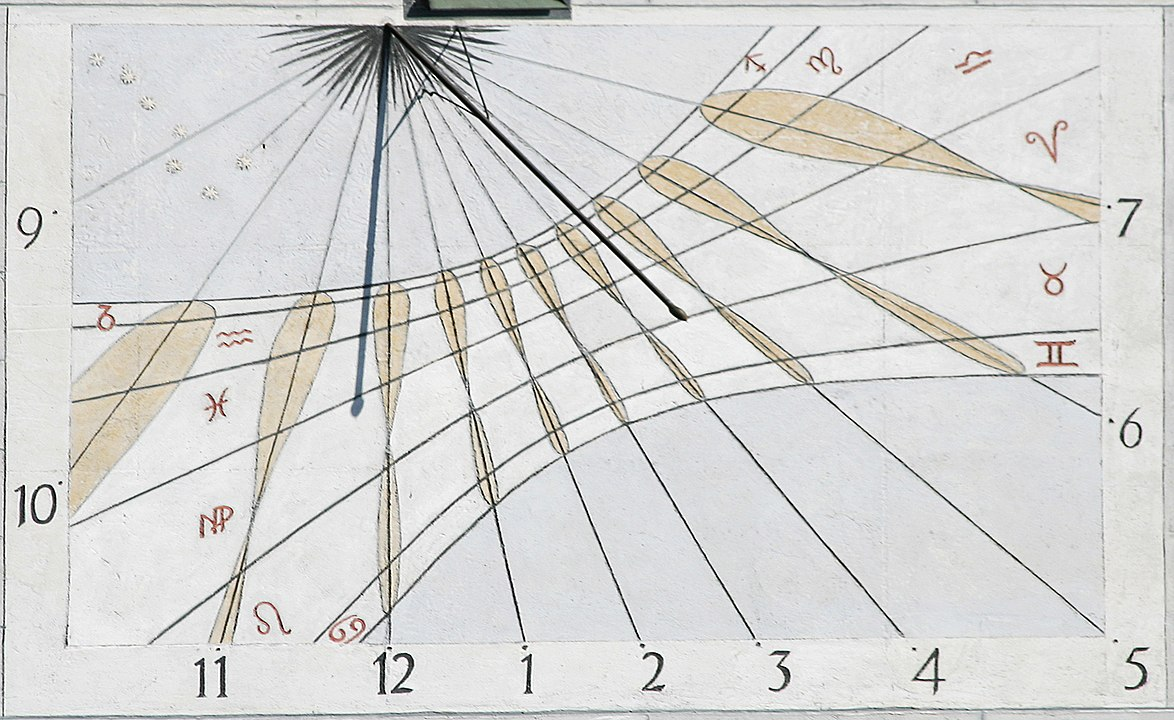
\includegraphics[scale=0.3]{./Bilder/Munich_Altes_Rathaus_sundial.jpg}
\caption{\label{fig_Munich_Analemma}%
Sonnenuhr am Alten Rathaus in M\"unchen. Anhand der Schattenl\"ange zu verschiedenen Jahreszeiten
kann die wahre (angezeigte) Uhrzeit um die Zeitgleichung korrigiert werden, die durch die
Analemmas an den Stundenlinien angegeben wird. Die Sternzeichen geben an, welcher
Teil des Analemmas (linker oder rechter Rand) in einem bestimmten Monat zu verwenden ist. (aus \cite{Niermann})} 
\end{figure}

Das Analemma ist gleichzeitig ein Bild der Sonnenst\"ande am Himmel: Macht man t\"aglich
zur selben mittleren Uhrzeit ein Bild vom Sonnenstand, so ergibt sich im Verlauf eines Jahres die Form
des Analemmas.  

\subsection{Wasseruhren und andere Zeitmesser des Altertums}

Ein Hilfsmittel zur Reproduktion gleicher Zeitr\"aume war auch die Klepshydra: 
ein mit Wasser\index{Klepshydra}\index{Wasseruhr}
gef\"ulltes Gef\"a\ss\ mit einer kleinen \"Offnung an der unteren Seitenwand oder im Boden, 
durch die das Wasser auslaufen
konnte, das dann in einem zweiten Gef\"a\ss\ aufgefangen wurde. Mit solchen Klepshydren wurden
beispielsweise die Redezeiten bei politischen Versammlungen oder auch bei Gerichtsprozessen im alten 
Griechenland und Rom
gemessen. Vermutlich geht hierauf der Begriff \glqq seine Zeit ist abgelaufen\grqq\ zur\"uck. Noch heute
beruht die Sanduhr, gelegentlich zum Eierkochen oder auch bei Gesellschaftspielen verwendet, 
auf diesem Prinzip.

Im fr\"uhen Mittelalter wurden die Klepshydren zu komplizierteren Wasseruhren abgewandelt. 
Dabei handelte es sich um teilweise sehr aufwendige Anlagen, durch die Wasser aus einem
oberen Reservoir in ein tiefer gelegenes Reservoir floss und dabei komplexe Mechanismen
in Gang setzte. Manche dieser Mechanismen glichen auch schon den sp\"ateren Hemmungen.

Insbesondere in Kl\"ostern, wo teilweise auch zu Nachtstunden zum Gebet aufgerufen wurde, kamen sp\"ater
sogenannte\index{Stundenkerze} 
Stundenkerzen - Kerzen genormter Dicke, bei denen Markierungen den groben
Stundenverlauf anzeigten - hinzu. Einem \"ahnlichen Zweck dienten auch \"Olkerzen, bei denen
ein Docht in ein mit \"Ol gef\"ulltes Gef\"a\ss\ ragte und am anderen Ende brannte. Die
verflossene Zeit konnte an dem verbrauchten \"Ol abgelesen werden.

\section{Uhren}

Um 1300 erlaubte die Erfindung der sogenannten Hemmung die Konstruktion der
ersten R\"aderuhren und damit von mechanischen Uhren, die auf oszillatorischen Prozessen beruhen. 
Wer den Mechanismus der Hemmung erfunden hat oder wann genau dieser
Mechanismus erfunden wurde, ist nicht bekannt. Wir wissen heute lediglich, dass um 1300 die
ersten Uhren entstanden sind, die auf diesem Prinzip beruhen. 

\subsection{Hemmungen}

Eine Hemmung\index{Hemmung} 
erlaubt es, eine mechanische Kraft (z.B.\ eine Gewichtskraft) in eine regelm\"a\ss ige Bewegung
umzuwandeln. H\"angt beispielsweise ein Gewicht an einem langen Seil, aufgewickelt auf eine
frei drehbare Rolle, so w\"urde ungehemmt das Gewicht mit wachsender Geschwindigkeit
absinken und die Rolle w\"urde sich mit zunehmender Geschwindigkeit drehen. Eine Hemmung
bewirkt, dass diese Drehung in eine meist abgehackte, konstant periodische Bewegung umgewandelt wird
und somit f\"ur eine Zeitmessung verwendet werden kann. Die \"altesten Hemmungen sind die
sogenannten Spindelhemmungen\index{Spindelhemmung}\index{Foliot} 
mit einem Foliot - einem hin und her schwingenden Querbalken mit Gewichten, 
der \"uber eine vertikale Achse mit zwei Pl\"attchen in ein Zahnrad\index{Kronrad} 
(das Kronrad) eingreift (siehe Abb.\ \ref{fig_Foliot}) - oder\index{Unrast}
einer Unrast, einer rotierende Scheibe, die ansonsten nach einem 
\"ahnlichen Mechanismus wie das Foliot arbeitet.

\begin{figure}[htb]
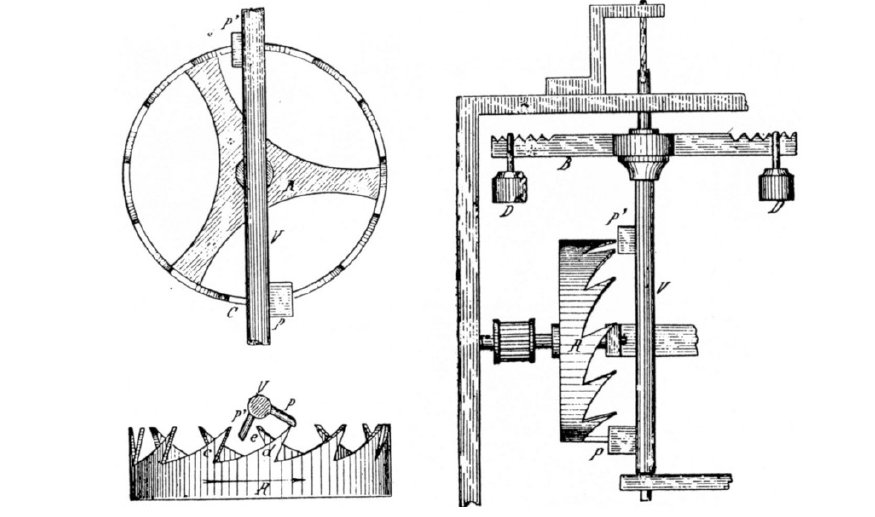
\includegraphics[scale=0.4]{./Bilder/Foliot.jpg}
\caption{\label{fig_Foliot}%
Eine Spindelhemmung mit Foliot. Das Kronrad $R$ wird \"uber ein Gewicht, das an einem \"uber die
Achse des Kronrads gewickelten Seil h\"angt (nicht dargestellt), angetrieben. Das Foliot $B$ mit den Gewichten $D$
besteht aus einem waagerechten Balken, der fest mit einer vertikalen Achse $V$ verbunden ist. 
An dieser Achse befinden sich zwei Pl\"attchen $P$ und $P'$, die abwechselnd oben und unten in die
Z\"ahne ($c$, $d$ und $e$) des Kronrads $R$ einhaken. 
Dies f\"uhrt zu einer Hin- und Herbewegung des Foliots und damit
zu einer kontrollierten, langsamen, abgehackt gleichm\"a\ss igen Drehung des Kronrads. \"Uber die Gewichte kann
die Schwingungsfrequenz des Foliots und damit der Gang der Uhr reguliert werden.
(aus \cite{Foliot})}
\end{figure}
 
 Ein Video mit dem Mechanismus einer Spindelhemmung findet man unter \cite{Verge}. 
 \"Uber Zahnradmechanismen, die im Mittelalter schon lange bekannt waren, 
 kann die Drehung des Kronrads auf andere R\"ader \"ubertragen und
 dabei beliebig verlangsamt werden. Bis zum 17.\ Jahrhundert erreichten Uhren mit Spindelhemmungen eine
 Genauigkeit von rund 15 Minuten pro Tag. 
 
 \subsection{Pendeluhren}

Im 17.\ Jahrhundert wurde die Spindelhemmung durch die mit einem Pendel gekoppelte 
Ankerhemmung\index{Ankerhemmung}\index{Pendeluhr}
ersetzt (siehe Abb.\ \ref{fig_Anker}). 
Nachdem Galileo\index{Galilei, Galileo} 
um 1630 festgestellt hatte, dass die Periode eines Pendels f\"ur kleine Auslenkungen 
nahezu unabh\"angig von dieser Auslenkung ist, erkannte man, dass sich das Pendel im Vergleich zum Foliot 
besser als Taktgeber eignet. Durch das Drehmoment, das \"uber ein Gewicht auf das Kronrad \"ubertragen
wird, gibt das Kronrad bei seinem Weiterdrehen \"uber den Anker umgekehrt dem Pendel regelm\"a\ss ig 
einen kleinen Sto\ss, sodass dieses 
mit einer kleinen aber konstanten Auslenkung schwingt und nicht durch Reibungseffekte zur Ruhe kommt. 

\begin{figure}[htb]

\includegraphics[trim=2 2 2 2,clip,scale=0.3]{./Bilder/Anker_10.png}

\includegraphics[trim=2 2 2 2,clip,scale=0.3]{./Bilder/Anker_18.png}

\includegraphics[trim=2 2 2 2,clip,scale=0.3]{./Bilder/Anker_27.png}

\includegraphics[trim=2 2 2 2,clip,scale=0.3]{./Bilder/Anker_35.png}
\caption{\label{fig_Anker}%
Eine Ankerhemmung. Der Anker ist fest mit einem Pendel verbunden, und wenn das Pendel schwingt, greift
der Anker abwechselnd rechts und links in die Zacken des Kronrads. Das Kronrad dreht sich im Uhrzeigersinn
und wird von einem Gewicht (nicht dargestellt) angetrieben. Bei jeder Vorw\"artsbewegung \"ubertr\"agt es 
aufgrund der Zackenform und der Form des Ankerhakens einen kleinen Sto\ss\ auf den Anker und damit auf
das Pendel. (aus \cite{Verge})}
\end{figure}

Christiaan Huygens\index{Huygens, Christiaan}\index{Hooke, Robert} 
entwickelte um 1656 eine Uhr auf dem Prinzip der Pendeluhr. Nachdem Robert Hooke
1658 die Ankerhemmung erfunden hatte, die eine kleine Schwingungsauslenkung des Pendels erm\"oglichte und damit
eine h\"ohere Genauigkeit in der Pendelperiode, wurde die Pendeluhr zum Standard in der Uhrenkonstruktion. 
Hier zeigt sich das Grundprinzip der heutigen Uhren: Eine harmonische Schwingung dient einerseits
als Standard f\"ur die Zeitmessung, andererseits wird sie durch den Mechanismus der R\"uckkopplung
von einer \"au\ss eren Kraft (hier das Gewicht, welches das Kronrad antreibt) aufrecht erhalten. 

\section{Das Problem des L\"angengrads}

Die Eroberung Konstantinopels\index{Konstantinopel} 
im Jahre 1453 durch die osmanischen Truppen markiert einen
entscheidenden Wendepunkt in der Geschichte des Abendlands. Oftmals wird in diesem Ereignis eine 
Ursache f\"ur den Wechsel vom Mittelalter zur Neuzeit gesehen. Diese Eroberung nach einer
langen Belagerung l\"oste zwei Bewegungen aus:
(1) Nachdem der Landweg von Europa zu den attraktiven Handelspl\"atzen in Indien, 
Indonesien und China im Wesentlichen gesperrt bzw.\ unter islamischer Kontrolle war, was oft
hohe Abgaben bzw.\ Z\"olle zur Folge hatte,
suchte man nach anderen Wegen nach Indien. Dies f\"uhrte nicht nur zur Umsegelung Afrikas,
sondern auf der Suche nach einem direkten Weg nach Indien auch zur Entdeckung Amerikas und
des Pazifischen Ozeans. (2) Die Flucht vieler Gelehrter aus Konstantinopel in den Westen,
die in ihrem Gep\"ack oft wertvolle B\"ucher mit sich f\"uhrten, l\"oste die\index{Renaissance}
Renaissance aus - auf diese Weise wurden viele antike Schriften, teilweise in ihren
arabischen \"Ubersetzungen, im Westen erst bekannt.  

Insbesondere die Erkundungsfahrten zur See brachten einige Probleme auf: Bis zu Beginn
des 15.\ Jahrhunderts beschr\"ankten sich Seefahrten haupts\"achlich auf den Mittelmeerraum
oder aber auf Fahrten entlang der europ\"aischen K\"usten nach Norden (Frankreich, England, 
Norwegen) oder entlang der afrikanischen K\"uste nach S\"uden (bei dieser Gelegenheit wurden
die Kanarischen Inseln sowie sp\"ater die Inselgruppe um Madeira und die Azoren entdeckt). Im Verlauf
des 15.\ Jahrhunderts erkundete man haupts\"achlich den Seeweg um Afrika nach Indien, der
dann von Vasco da Gama\index{Vasco da Gama} 
im Jahre 1498 auch gefunden wurde und eine Route von
Europa nach Indien und China er\"offnete, die nicht durch islamisch
kontrolliertes Gebiet f\"uhrte. Eine solche Umsegelung Afrikas war
m\"oglich, ohne \"uber einen l\"angeren Zeitraum hinweg die K\"uste als Anhaltspunkt f\"ur die
Ortsbestimmung aus dem Blickfeld zu verlieren. Allerdings war diese Schiffsroute sehr lang
und wegen der vielen Piraten in der N\"ahe des Horns von Afrika auch recht gef\"ahrlich.

Die andere M\"oglichkeit sah man in einer direkten Route von Europa nach Indien auf einem Weg
in Richtung Westen.\index{Columbus, Christoph} 
Diesen Weg wollte Columbus finden und entdeckte auf diese Weise
1492 das heutige Amerika (genauer entdeckte er eine Insel der Bahamas). W\"ahrend eine Umfahrung Afrikas
noch mit visuellem K\"ustenkontakt m\"oglich war, musste man f\"ur die Westroute die
vertrauten K\"usten Europas und Afrikas verlassen. Nachdem Columbus die Bahamas entdeckt hatte 
und in der Folgezeit auch L\"ander auf dem amerikanischen Festland
(sowohl in Nord- als auch S\"udamerika) entdeckt wurden, und nachdem 
Ferdinand Magellan\index{Magellan, Ferdinand} 
um 1520 die erste Umsegelung S\"udamerikas und die \"Uberquerung des Pazifischen Ozeans
gelang, wurde das Problem der genauen Ortsbestimmung der neu entdeckten L\"ander und
Inseln wichtig. Zum Einen wollten die Herrscher, die solche Erkundungsfahrten der Seefahrer
finanzierten und die dabei entdeckten L\"ander f\"ur sich in Anspruch nahmen, wissen, wo 
genau sich diese L\"ander befanden, d.h.\ es kam die Frage auf, wie man diese L\"ander wiederfinden kann. 
Zum Anderen war es auch f\"ur Seefahrer wichtig zu wissen, wo genau man sich
befand, um beispielsweise bei Unwetter oder in der Nacht zu vermeiden, auf Felsen oder
Land aufzulaufen. 

Eine Bestimmung des Breitengrads\index{Breitengrad} 
war auch auf See mit hinreichender Genauigkeit
m\"oglich, sofern das Wetter es zulie\ss. Entweder konnte man bei Tag den Sonnenh\"ochststand oder
bei Nacht die Sterne beobachten und ausmessen. Der H\"ochststand der Sonne bei
Tag oder beispielsweise die H\"ohe des Polarsterns bei Nacht erlaubten eine direkte
Messung des Breitengrads. Problematischer war die Bestimmung des 
L\"angengrads:\index{Laengengrad@L\"angengrad}\index{Laengengradproblem@L\"angengradproblem}
Hierzu musste man entweder eine direkte Messung vornehmen, d.h.\ man bestimmte die zur\"uckgelegte
Strecke aus der Geschwindigkeit des Schiffs und der Reisedauer  -  auf See war das nur
bei ruhigem Wetter und ruhiger See (ohne Str\"omungen) m\"oglich - oder man musste 
die genaue Uhrzeit an einem Referenzpunkt, dessen L\"angengrad bekannt war, kennen.
 
Eine dritte M\"oglichkeit, die vermutlich bei den ersten Pazifik\"uberquerungen verwendet wurde,
bestand darin, unter einem konstanten Winkel zum L\"angengrad (im 16.\ Jahrhundert gab es
schon recht gute Magnetkompasse sowie Kenntnisse zu den Abweichungen zwischen
magnetischem und geographischen Nordpol) zu segeln und dann aus der \"Anderung des
Breitengrads auf die \"Anderung im L\"angengrad zu schlie\ss en. Dieses Verfahren funktioniert
nicht bei einer reinen Ost-West-Fahrt, also entlang eines konstanten Breitengrads. Solche Routen
wurden gerne verwendet, da sich der Breitengrad leicht bestimmen lie\ss\ und diese
Routen somit gut reproduzierbar waren.

Direkte Messungen waren schwierig, da der Fehler kumulativ ist (d.h., kleine Fehler in den 
Messungen - insbesondere systematische Fehler - 
addieren sich \"uber einen l\"angeren Zeitraum hinweg zu
einem gro\ss en Fehler) und daher sehr anf\"allig f\"ur Ungenauigkeiten, beispielsweise
bei nicht idealen Wetterverh\"altnissen oder Meeresstr\"omungen, die es schwer bis unm\"oglich
machten, die Geschwindigkeit des Schiffs zu bestimmen. 
Daher sah man die L\"osung nur in einer genauen
Zeitmessung: Wenn man an einem bestimmten Ort den genauen Zeitpunkt des
Sonnenh\"ochststands misst und mit der gleichzeitigen lokalen Zeit an einem Referenzort
(z.B.\ dem Heimathafen) vergleicht, kann man aus der Zeitdifferenz den L\"angengrad des momentanen
Orts bestimmen. 

Da sich die Erde in 24 Stunden einmal um ihre Achse dreht, ein Ort am \"Aquator in dieser Zeit somit
40\,000\,km \glqq zur\"ucklegt\grqq, entspricht dies pro Minute einer Strecke von $27,\bar{7}$\,km. 
Ein L\"angengrad am \"Aquator entspricht rund 111,11\,km, und eine L\"angenminute rund 1\,852\,m,
einer nautischen Meile.\index{Meile!nautische}\index{Seemeile} 
F\"ur eine angestrebte Genauigkeit im Bereich von 5 bis 10 Kilometern bzw.\ eine L\"angengradmessung
mit einem Fehler zwischen 3 und 5 Bogenminuten musste die Zeit also auf
rund 15 Sekunden bekannt sein. Das war mit den Uhren im sp\"aten Mittelalter oder der fr\"uhen
Neuzeit kaum m\"oglich. Selbst unter idealen Bedingungen auf festem Boden in abgeschlossenen
R\"aumen erreichte man mit den Pendeluhren\index{Pendeluhr} 
im 17.\ Jahrhundert bestenfalls eine Genauigkeit von
15 Sekunden am Tag. Auf hoher See, wo das Schiff St\"urmen ausgesetzt war oder auch extremen
Temperatur- und Feuchtigkeitsschwankungen, eine Genauigkeit von 15 Sekunden \"uber einen l\"angeren
Zeitraum (von z.B.\ 10--14 Tagen) zu erreichen, schien Anfang des 18.\ Jahrhunderts noch unm\"oglich.
Nachdem bei einem gro\ss en Seeungl\"uck der englischen Flotte im Jahre 1707 bei den Scilly Islands 
fast 2000 Seeleute ums Leben gekommen waren und vier Schiffe zerst\"ort wurden, was
auf eine fehlerhafte Ortsbestimmung des Kapit\"ans zur\"uckging, setzte die britische Regierung im
sogenannten \textit{Longitude Act}\index{Longitude Act} 
1714 eine Belohnung von letztendlich insgesamt 20\,000 englischen Pfund (das entspricht
heute rund 1,5--2\,Millionen Euro) aus f\"ur denjenigen, der das Problem der Messung des L\"angengrads
auf eine einfache und praktische Weise l\"osen konnte. 

Zwei Ans\"atze wurden in diesem Zusammenhang verfolgt: (1) Die Erstellung sehr genauer Ephemeridentafeln 
(z.B.\ auch von den Jupitermonden) und (2) die Konstruktion einer Uhr, die \"uber einen l\"angeren Zeitraum
auch unter den Bedingungen auf See eine Ortsbestimmung auf wenige Kilometer erm\"oglichte. Der erste
Ansatz f\"uhrte im 18.\ Jahrhundert zur Einrichtung vieler Sternwarten, unter anderem auch der
Sternwarte von Greenwich. Auch die Arbeiten Newtons zur Himmelsmechanik k\"onnen vor dem 
Hintergrund des L\"angengradproblems gesehen werden. Der zweite, letztendlich erfolgreiche Ansatz
war die Konstruktion von Chronometern,\index{Chronometer}\index{Harrison, John} 
also sehr genauen und gegen \"au\ss ere Einfl\"usse weitgehend
unempfindlichen Uhren, insbesondere der sogenannten 
H4 und H5 von John Harrison, der nach langem Kampf
um 1775 einen Gro\ss teil des Preisgelds in Empfang nehmen durfte. Eine ausf\"uhrliche und sehr lesbare
Schilderung des L\"angengradproblems und seiner L\"osung findet man in dem Buch von Dava Sobel \cite{Sobel}.

\section{Moderne Uhren}

Da es hier nicht um eine ausf\"uhrliche Darstellung der Geschichte der Zeitmessung gehen soll, seien
nur die wichtigsten Entwicklungen im 19.\ und 20.\ Jahrhundert erw\"ahnt. 

Um 1850 entstanden die
ersten elektrischen Uhren, bei denen die Anregung der Schwingung nicht mehr mechanisch \"uber
das langsam herabsinkende Gewicht gesteuert wurde, sondern durch einen elektrischen Strom, beispielsweise
aus einer Batterie. Zwei Entwicklungen f\"uhrten dabei zu den heutigen Atomuhren: (1) die Einf\"uhrung des
\glqq Master-Slave-Prinzips\grqq,\index{Master-Slave-Prinzip} 
bei dem Taktgeber - der Mechanismus, \"uber den die Uhrzeit gemessen 
wird - und Takthalter - der Mechanismus, der f\"ur eine m\"oglichst gleichm\"a\ss ige Schwingung sorgt - 
getrennt wurden, was zu einer
besseren Genauigkeit f\"uhrte, und (2) die Ausnutzung von zun\"achst Kristallschwingungen (die Quarzuhr)
und sp\"ater atomaren Schwingungen (die Atomuhr).  

\subsection{Das Master-Slave-Prinzip}

In den alten mechanischen Uhren, beispielsweise den Pendeluhren der fr\"uhen Neuzeit, diente
der periodische Prozess - das Schwingen des Pendels - sowohl zur Vorgabe einer m\"oglichst gleichm\"a\ss igen
Taktzeit, als auch zum Ablesen der Uhrzeit. Die Hemmung, beispielsweise die Ankerhemmung, \"ubertrug
dem Pendel bei jedem Takt eine minimale Energie von dem Kronrad, das durch ein Gewicht in Drehung
versetzt wurde, sodass das Pendel nicht zur Ruhe kam. Gleichzeitig diente das sich drehende Kronrad aber auch 
als Ausgangspunkt f\"ur die rotierenden Zeiger der Uhr. Dieser Mechanismus war anf\"allig f\"ur St\"orungen
und minimale Schwankungen.

Bei Master-Slave-Prinzip (zum ersten Mal umgesetzt in einer sogenannten 
Shortt-Uhr, benannt nach dem\index{Shortt-Uhr}\index{Shortt, William Hamilton}
englischen Ingenieur William Hamilton Shortt) gibt es einen
Takthalter, ein sogenanntes Prim\"arpendel, das m\"oglichst st\"orungsfrei dieselbe Schwingungsperiode h\"alt, und
einen f\"ur das Ablesen der Uhrzeit bestimmten Taktgeber, in diesem Fall ein sogenanntes Sekund\"arpendel, \"uber
dessen Bewegung ein Zeigerwerk in Gang gesetzt wird, an dem die Uhrzeit abgelesen werden kann. 
Das Prim\"arpendel befand sich bei der Shortt-Uhr in einem Vakuumzylinder, es erhielt in regelm\"a\ss igen
(aber seltenen) Abst\"anden einen wohldefinierten Impuls und sandte, ebenfalls in regelm\"a\ss igen nicht zu
h\"aufigen Abst\"anden ein elektrisches Signal an das Sekund\"arpendel, das auf diese Weise gesteuert wurde
und im selben Takt wie das Prim\"arpendel schwang. Durch den Ablesemechanismus und andere \"au\ss ere
Einfl\"usse konnte das Sekund\"arpendel zwar in seiner Bewegung gest\"ort werden, durch die regelm\"a\ss igen
Pulse des Prim\"arpendels wurde es aber immer wieder in Phase zum Prim\"arpendel gebracht. 

Dieses Prinzip - es wird nicht die Schwingung des Prim\"aroszillators ausgelesen sondern die Schwingung
eines Sekund\"aroszillators, der von dem Prim\"aroszillator gesteuert wird - findet sich auch in sp\"ateren 
Pr\"azissionsuhren, beispielsweise auch den heutigen Atomuhren. Die Shortt-Uhren waren die ersten
mechanischen Uhren, mit denen um 1930 Schwankungen in der Erdrotation und damit Schwankungen in der
mittleren Tagesl\"ange nachgewiesen werden konnten. 

\subsection{Quarzuhren}

1927 wurde die erste Quarzuhr\index{Quarzuhr} 
vorgestellt. Nachdem um 1880 von den Br\"udern Jacques und
Pierre Curie die Piezoelektrizit\"at entdeckt worden war - also dass die Anlegung einer Spannung
an manche Kristalle zu einer leichten Verformung dieser Kristalle f\"uhrt, und umgekehrt, dass eine mechanische
Verformung der Kristalle eine Spannung erzeugt - gelang es in den 20er Jahren des 20.\ Jahrhunderts,
diese im Hochfrequenzbereich zur Erzeugung von Quarzschwingungen und zum Auslesen dieser
Schwingungen zu nutzen und damit die ersten Quarzuhren zu konstruieren. Den gr\"o\ss ten Einfluss
auf die Genauigkeit hatte ihre Temperaturempfindlichkeit, die in den n\"achsten Jahren zunehmend unter
Kontrolle gebracht werden konnte.  

\subsection{Atomuhren}

Atomuhren\index{Atomuhr} 
nutzen die harmonischen Schwingungen im Zusammenhang mit \"Uberg\"angen zwischen
atomaren Zust\"anden. Bei den \"alteren Atomuhren, einschlie\ss lich den C\"asium-Uhren, handelt es sich dabei
um \"Uberg\"ange im Radiowellenbereich, meist \"Uberg\"ange zur Hyperfeinstruktur. Sowohl bei
Wasserstoff-Uhren als auch C\"asium-Uhren betrachtet man den 
Hyperfeinstruktur\"ubergang\index{Hyperfeinstruktur\"ubergang} 
zwischen zwei elektronischen Spinzust\"anden relativ zum Kernspin: Die Atome haben ein einzelnes
Elektron in der \"au\ss eren Schale, dessen Spin parallel oder antiparallel zum Kernspin sein kann. 
Die Energie zwischen diesen beiden Zust\"anden unterscheidet sich nur minimal und entspricht
langwelligen Strahlungen: Bei Wasserstoff handelt es sich um die in der Astronomie bekannte
21-cm-Strahlung - der \"Ubergang entspricht einer Frequenz von 1\,420\,MHz bzw.\ einer Energie
von $5,87\,\mu{\rm eV}$ und somit hat
die Strahlung im Vakuum eine Wellenl\"ange von 21\,cm - und bei C\"asium handelt es sich um die
zu Beginn dieses Kapitels angegebenen Werte. 

C\"asium hat mehrere Vorteile:\index{Caesium@C\"asium} 
Einerseits gibt es von C\"asium nur ein stabiles Isotop (Cs-133), sodass
der Einfluss unterschiedlicher Isotope in einer Probe vernachl\"assigt werden kann, C\"asium hat ein einzelnes Elektron
in seiner \"au\ss eren Schale und sein Siedepunkt ist mit rund $690^\circ$C vergleichsweise niedrig. Schon bei
rund $100{\,}^\circ$C gibt es thermisch verdampfende Atome, die sich f\"ur den Betrieb einer Atomuhr eignen.

\begin{figure}[htb]
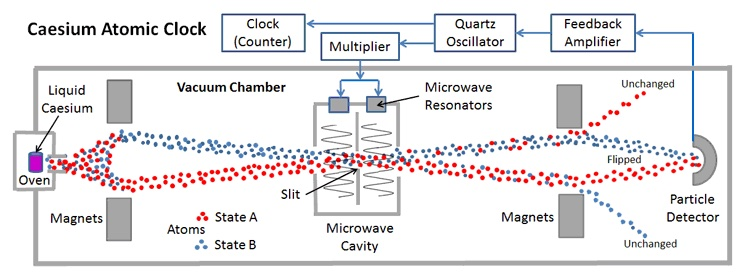
\includegraphics[scale=0.5]{./Bilder/Atomic_Clock.jpg}
\caption{\label{fig_Atomuhr}%
Prinzip einer C\"asium-Uhr: Aus einem Ofen str\"omen C\"asium-Atome nahezu gleichverteilt im
Grundzustand und im angeregten Hyperfeinstrukturzustand. In einem Magnetfeld werden die
Atome im Grundzustand von denen im angeregten Zustand getrennt (sie haben unterschiedliche
magnetische Momente) und treten dann unter einem unterschiedlichen Winkel in einen
Resonator. In diesem Resonator werden sie einem oszillierenden Feld ausgesetzt, dessen Frequenz
\"uber eine R\"uckkopplung auf die Eigenfrequenz des \"Ubergangs eingestellt wird. Dadurch werden die
Atome zu \"Uberg\"angen angeregt. In einem Detektor hinter dem Resonator wird die Anzahl der Atome
gemessen, die einen \"Ubergang gemacht haben - je genauer die Resonatorfrequenz auf die
\"Ubergangsfrequenz eingestellt ist, umso mehr Atome werden zu einem \"Ubergang angeregt. Der
Detektor steuert \"uber die R\"uckkopplung die Frequenz des Resonators, sodass m\"oglichst viele
Atome den Detektor erreichen. Abgelesen wird die Frequenz des Resonators. (aus \cite{Atomuhr})}   
\end{figure}

In einem Resonator werden die C\"asiumatome zu \"Uberg\"angen angeregt (Abb.\ \ref{fig_Atomuhr}), wobei
der Anteil der Atome, die einen \"Ubergang machen, umso h\"oher ist, je n\"aher die Frequenz des
Resonatorfeldes an der \"Ubergangsfrequenz liegt. Die Frequenz des Resonatorfeldes wird von einem
Quarzkristall gesteuert, der wiederum von einem Detektor hinter dem Resonator gesteuert wird. 
Dieser Detektor misst die Anzahl der Atome, die einen \"Ubergang gemacht haben, und er steuert den
Quarzkristall so, dass diese Anzahl maximal bleibt. An dem Quarzkristall wird dann auch die jeweilige
Frequenz abgelesen und in eine Uhrzeit umgewandelt. 

Moderne\index{Opticlock} 
Atomuhren arbeiten bei optischen Frequenzen und erreichen damit nochmals eine um
einen Faktor 1000 bis 10\,000 h\"ohere Genauigkeit. Sie befinden sich derzeit in der Testphase,
es wird aber nicht ausgeschlossen, dass in einigen Jahren die Sekunde \"uber solche Opticlocks
neu festgelegt wird. 

\subsection{Fountain-Clocks}

Das bisher beschriebene Verfahren beruht auf Ideen von Isidor Isaac Rabi Mitte des letzten Jahrhunderts.
Diese Ideen wurden von seinem \glqq Sch\"uler\grqq\ Norman Ramsey nochmals erweitert und zu gr\"o\ss erer
Pr\"azision gef\"uhrt. Eine wesentliche Verbesserung besteht darin, die Cs-Atome zweimal f\"ur einen
kurzen Augenblick durch einen Resonator zu schicken, wobei die Pr\"azession der Uhr umso gr\"o\ss er ist, je
mehr Zeit zwischen diesen beiden Augenblicken liegt.\index{Fountain-Clock} 
In sogenannten Fountain-Clocks (\glqq Springbrunnen-Uhren\grqq)
werden die C\"asiumatome zun\"achst abgek\"uhlt (d.h.\ verlangsamt, dies geschieht mit Laserk\"uhlung) 
und dann mit wenigen Metern pro
Sekunde senkrecht nach oben gesto\ss en. Sie durchlaufen in einem freien Fall eine Parabelkurve, wobei
sie zu Beginn und am Ende kurz durch einen Resonator fliegen. Auf diese Weise befinden sich die C\"asiumatome 
wesentlich l\"anger in der Phase zwischen den Resonatoreinfl\"ussen und die Genauigkeit der Frequenz 
kann besser reguliert werden. 

\section{Kuriosit\"aten}

\subsection{Die tautochrone Kurve - Zykloide}

Nachdem Galilei erkannt hatte, dass bei einem Pendel die Periode bei kleinen Auslenkungen
nahezu unabh\"angig von der Amplitude des Pendels ist, hatte 
Christiaan Huygens\index{Huygens, Christiaan} 
1656 die Idee, ein Pendel als Taktgeber einer Uhr zu verwenden. Ihm war jedoch
bewusst, dass bei einem realen Pendel die Periode nicht vollkommen unabh\"angig von der Auslenkung
ist und bei gro\ss en Auslenkungen doch deutliche Abh\"angigkeiten von der Amplitude auftreten.
Huygens stellte sich daraufhin die Frage, wie man erreichen kann, dass die Periodendauer eines
Pendels vollkommen unabh\"angig von der Auslenkung ist. 

Das theoretische Problem besteht zun\"achst darin, die Bahnkurve zu bestimmen, die ein
Massenpunkt durchlaufen muss, sodass die Periode der Schwingung unabh\"angig von der Auslenkung ist.
Eine solche Bahnkurve bezeichnet man als\index{tautochron}\index{isochron} 
tautochrone oder auch isochrone Bahnkurve.
Eine Kreiskurve, wie sie bei einem Pendel konstanter Pendell\"ange durchlaufen wird, hat diese 
Eigenschaft nur bis auf Terme 4.\ Ordnung in der Auslenkung (z.B.\ im Auslenkungswinkel) und daher
nur f\"ur kleine Auslenkungen. Das
zweite, eher praktische Problem besteht in der Konstruktion eines Aufh\"angemechanismus,
sodass die Masse an einem Fadenpendel tats\"achlich die tautochrone Bahnkurve durchl\"auft.

Man kann analytisch mit Variationsrechnung die Form dieser Bahnkurve herleiten. Wir geben hier jedoch das 
Ergebnis an und beweisen, dass diese Bahnkurve die gew\"unschten Eigenschaften hat. 
Es handelt sich um\index{Zykloide}
eine sogenannte Zykloide, wie sie in Abb.\ \ref{fig_Zykloide} dargestellt ist. Eine Zykloide wird von einer
Markierung am Rand eines Kreises beschrieben, wenn dieser Kreis an einer Geraden entlang rollt. 

\begin{figure}[htb]
\begin{tikzpicture}
\draw (9.5,2) circle (2.0cm);
\draw (7.28,2) circle (2.0cm);
\draw [->] (0,4) -- (15,4);
\draw (14.7,3.9) node{${\scriptstyle x}$}; 
\draw [->] (7.28,4) -- (7.28,-1);
\draw (7.4,-0.8) node{${\scriptstyle y}$}; 
\draw (9.5,4) -- (9.5,0);
\draw (7.72,2.9) -- (11.28,1.1);
\draw (9.5,4) -- (11.28,1.1);
\draw (9.5,0) -- (13.5,2.46);
\draw (11.28,1.1) -- (13.5,1.1);
\draw (11.28,1.1) -- (9.5,1.1);
\filldraw[fill=red] (1,4) circle(0.08cm);
\draw (1,4.2) node{${\scriptstyle A}$}; 
\filldraw[fill=red] (13.57,4) circle(0.08cm);
\draw (13.57,4.2) node{${\scriptstyle D}$}; 
\filldraw[fill=black] (7.28,4) circle(0.05cm);
\draw (7.28,4.2) node{${\scriptstyle E}$}; 
\filldraw[fill=red] (7.28,0) circle(0.08cm);
\draw (7.4,-0.2) node{${\scriptstyle B}$}; 
\filldraw[fill=red] (11.28,1.1) circle(0.08cm);
\draw (11.35,0.9) node{${\scriptstyle C}$}; 
\filldraw[fill=black] (7.72,2.9) circle(0.05cm);
\draw (7.98,3.0) node{${\scriptstyle E'}$}; 
\filldraw[fill=black] (9.5,2) circle(0.05cm);
\draw (9.28,1.83) node{${\scriptstyle M'}$}; 
\filldraw[fill=black] (7.28,2) circle(0.05cm);
\draw (7.1,2.0) node{${\scriptstyle M}$}; 
\filldraw[fill=black] (9.5,4) circle(0.05cm);
\draw (9.5,4.2) node{${\scriptstyle F}$}; 
\filldraw[fill=black] (9.5,1.1) circle(0.05cm);
\draw (9.3,1.1) node{${\scriptstyle G}$}; 
\draw (13.0,2.0) node{${\scriptstyle t}$}; 
\draw (4.0,4.13) node{${\scriptstyle a}$}; 
\draw (10.4,1.4) node{${\scriptstyle r}$}; 
\draw (7.12,1) node{${\scriptstyle r}$}; 
\draw (11.7,1.23) node{${\scriptstyle \theta}$}; 
\draw[thick] (1,4) .. controls (1,2.9) and (3.17,0) .. (7.28,0); 
\draw[thick] (7.28,0) .. controls (11.4,0) and (13.57,2.9) .. (13.57,4); 
\draw (7.28,4) .. controls (7.28,3.6) and (7.4,3.2) .. (7.72,2.9); 
\draw (9.65,1.8) node{${\scriptstyle \alpha}$}; 
\draw (9.38,2.2) node{${\scriptstyle \alpha}$}; 
\draw (9.6,3.6) node{${\scriptstyle \theta}$}; 
\draw (11.0,1.4) node{${\scriptstyle \theta}$}; 
\draw (9.65,2.12) node{${\scriptstyle \gamma}$}; 
\draw (9.5,1.6) arc (270:515:0.4cm);
\draw (9.5,3.4) arc (270:300:0.6cm);
\draw (10.98,1.58) arc (115:150:0.5cm);
\draw (11.9,1.1) arc (0:30:0.6cm);
\end{tikzpicture}
\caption{\label{fig_Zykloide}%
Die Zykloide. Wenn ein Kreis (Radius $r$) auf einer geraden Linie $a$ (gleichzeitig die $x$-Achse)
abrollt, beschreibt ein Punkt $B$ auf dem
Rand des Kreises (rot eingezeichnet) den Bogen einer Zykloide. Es gilt immer $\alpha=2\theta$, da
sowohl $\alpha + \gamma$ als auch $\gamma + 2\theta$ einem Winkel von $180^\circ$ entsprechen.
Die Tangente $t$ im Punkt $C$ steht senkrecht auf der Verbindungslinie $\overline{FC}$ und schlie\ss t
mit einer Waagerechten einen Winkel $\theta$ ein. Der Nullpunkt des Koordinatensystems sei der
Punkt $E$. Wenn der Kreis in diesem Punkt die Achse $a$ ber\"uhrt, sei $B$ am Minimum der Kurve, also
auf dem Kreis dem Punkt $E$ gegen\"uber.} 
\end{figure}

Wir w\"ahlen den Nullpunkt unseres Koordinatensystems als den Ber\"uhrungspunkt $E$ des Kreises mit der
Geraden an der Stelle, wo die Markierung (Punkt $B$) im Mininum ist. Rollt der Kreis
um einen Winkel $\alpha$ nach rechts, ist der Ber\"uhrungsgpunkt mit der Geraden der Punkt $F$. Die
Distanz zwischen $E$ und $F$ ist genau gleich der Bogenl\"ange zwischem dem ehemaligen Ber\"uhrunsgpunkt
(jetzt $E'$) und dem Punkt $F$, also $\overline{EF}=\alpha r$, wobei der Winkel $\alpha$ in Radianten ausgedr\"uckt
wird. Der Punkt $B$ hat sich bis zum Punkt $C$ weiterbewegt und dabei den
Bogenabschnitt der Zykloide \"uberstrichen.

Wir geben zun\"achst eine Parametrisierung der Zykloide an: Die $x$- und die $y$-Koordinate werden als
Funktion des Winkels $\alpha\in [-\pi,+\pi]$ beschrieben:
\begin{equation}
        x(\alpha) = r ( \alpha + \sin \alpha )    \hspace{1cm} , \hspace{1cm}   y(\alpha) = - r (1+  \cos \alpha ) \, .
\end{equation}
Die $x$-Koordinate ergibt sich aus der Summe von zwei Beitr\"agen: $\overline{EF}+\overline{GC}=r\alpha + r\sin \alpha$,
und die $y$-Koordinate ergibt sich aus: $\overline{FM'} + \overline{M'G}=r + r\cos \alpha$ (in die negative $y$-Richtung). 

Zum Beweis, dass die Zykloide tats\"achlich  die L\"osung des Problems darstellt, ist zu zeigen, dass die
Kraft proportional zur Bogenl\"ange der Auslenkung ist, dass es sich also um einen idealen harmonischen Oszillator
handelt. Dies unterscheidet die Zykloide von einer Parabel: Bei einer Parabel ist die Kraft proportional
zur Auslenkung in $x$-Richtung (oder, was \"aquivalent ist, das Potenzial ist proportional zum Quadrat der 
Auslenkung in $x$-Richtung), bei einer Zykloide ist die Kraft proportional zur Bogenl\"ange. Die Richtung der 
Kraft ist tangential zur Kurve und somit ist 
\begin{equation}
        F=mg \sin \theta=mg \sin \frac{\alpha}{2} \, .
\end{equation} 

Die Bogenl\"ange entlang der Zykloide (also zwischen $B$ und $C$) erhalten wir aus
\begin{eqnarray}
   {\rm d}s^2 &=& \left( \left( \frac{{\rm d} x}{{\rm d}\alpha} \right)^2 + \left( \frac{{\rm d} y}{{\rm d}\alpha} \right)^2 \right) 
                                     ({\rm d}\alpha)^2 \\ 
       &=&  \left( r^2 (1 + \cos \alpha)^2 + r^2 (\sin \alpha)^2 \right) ({\rm d}\alpha )^2 \\
       &=&   2 r^2 ( 1 + \cos \alpha) ({\rm d}\alpha )^2 \, .
\end{eqnarray}
Mit der trigonometrischen Beziehung
\begin{equation}
   1 + \cos \alpha = 1 + \cos^2 \frac{\alpha}{2} - \sin^2 \frac{\alpha}{2} = 2 \cos^2 \frac{\alpha}{2} 
\end{equation}
folgt
\begin{equation}
      {\rm d}s = 2r \cos \left( \frac{\alpha}{2} \right) \,  {\rm d} \alpha 
\end{equation}
und damit
\begin{equation}
      s = 2 r \int_0^\alpha \cos \left( \frac{\alpha'}{2} \right) \,  {\rm d} \alpha' = 
            4r  \left. \sin \frac{\alpha'}{2} \right|_0^\alpha = 4r \sin \frac{\alpha}{2}   \, .
\end{equation}
F\"ur die Zykloide gilt also tats\"achlich, dass die Bogenl\"ange proportional zur r\"ucktreibenden
Kraft ist und damit handelt es sich um einen idealen harmonischen Oszillator mit einer von der
Auslenkung unabh\"angigen Periode. 

\begin{SCfigure}[50][htb]
\begin{tikzpicture}[scale=0.5]
\draw (0,4) -- (14.6,4);
\draw [thick] (7.28,4) -- (7.28,-4);
\fill[gray!20!white]  (1,4) -- (1,0) .. controls (5.12,0) and (7.28,2.9) .. (7.28,4) -- (1,4); 
\fill[gray!20!white]  (7.28,4) .. controls (7.28,2.9) and (10.24,0) .. (13.56,0) -- (13.56,4) -- (7.28,4); 
\draw (1,0) .. controls (5.12,0) and (7.28,2.9) .. (7.28,4); 
\draw [thick] (7.28,4) .. controls (7.28,2.9) and (10.24,0) .. (13.56,0); 
\filldraw[fill=black] (7.28,4) circle(0.05cm);
\filldraw[fill=black] (7.28,-4) circle(0.1cm);
\filldraw[fill=black] (13.56,0) circle(0.1cm);
\draw [thick] (12.42,-2) -- (8.24,2.4);
\draw [thick] (7.28,4) .. controls (7.28,3.7) and (7.4,3.3)  .. (8.24,2.4);
\filldraw[fill=black] (12.42,-2) circle(0.1cm);
%
\draw (1,0) .. controls (1,-1.1) and (3.17,-4) .. (7.28,-4); 
\draw (7.28,-4) .. controls (11.4,-4) and (13.57,-1.1) .. (13.57,0); 
\end{tikzpicture}
\caption{\label{fig_Zykloide2}%
Die Huygens'sche Aufh\"an\-gung. Die Zykloide l\"ost gleichzeitig das zweite Problem bez\"uglich eines
von der Auslenkung unabh\"angigen Pendels: Wenn das schwingende Pendel an seiner Aufh\"angung
durch eine Zykloide begrenzt ist, sodass der obere Teil des Pendelseils an der Zykloide entlang
l\"auft, folgt die Masse am Ende des Pendels einer Zykloide.} 
\end{SCfigure}

Das zweite Problem des Huygens'schen Pendels, die Aufh\"angung, wird ebenfalls durch die Zykloide
gel\"ost.\index{Huygens'sche Pendelaufh\"angung} 
Abbildung \ref{fig_Zykloide2} zeigt, wie man die Aufh\"angung eines Pendels durch eine Zykloide
eingrenzen kann, sodass die Pendelmasse tats\"achlich die Trajektorie einer Zykloide durchl\"auft. 
Dies bezeichnet man auch als die Huygens'sche Pendelaufh\"angung.


Huygens erhoffte sich durch einen solchen Mechanismus
eine tautochrone Schwingung des Pendels auch unter extremen Bedingungen (z.B.\ auf einem
dem Wind und Wellen ausgesetzten Schiff). Letztendlich war diese Idee nicht erfolgreich, statt dessen wurden bessere
Hemmungen, die unter anderem kleinere Auslenkungen erm\"oglichten, entwickelt. 

\begin{thebibliography}{99}

\bibitem{Niermann} 
Till Niermann - Eigenes Werk, CC BY-SA 3.0, \url{https://commons.wikimedia.org/w/index.php?curid=21792620}

\bibitem{Atomuhr} aus: Electropaedia ``Clock and Watch Movements'', 
           \url{https://mpoweruk.com/timekeepers.htm}
\bibitem{Foliot} aus Wikipedia ``Foliot''. \url{https://de.wikipedia.org/wiki/Foliot#/media/Datei:Foliot.jpg}.
\bibitem{Verge} Spindel-Hemmung; \url{https://www.youtube.com/watch?v=UhFPb-ZZTyI}
\bibitem{Neugebauer} O.\ Neugebauer; \textit{A History of Ancient Mathematical Astronomy}, 
       Studies in the History of Mathematics and Physical Sciences 1; Springer-Verlag Berlin
       Heidelberg GmbH, 1975.
\bibitem{Sobel} Dava Sobel; \textit{Longitude}, Fourth Estate, Second Printing 1995. Deutsch: \textit{L\"angengrad};
                  Malik, National Geographic, 2013.        
\end{thebibliography}

%\end{document}


%\documentclass[german,10pt]{book}      
\usepackage{makeidx}
\usepackage{babel}            % Sprachunterstuetzung
\usepackage{amsmath}          % AMS "Grundpaket"
\usepackage{amssymb,amsfonts,amsthm,amscd} 
\usepackage{mathrsfs}
\usepackage{rotating}
\usepackage{sidecap}
\usepackage{graphicx}
\usepackage{color}
\usepackage{fancybox}
\usepackage{tikz}
\usetikzlibrary{arrows,snakes,backgrounds}
\usepackage{hyperref}
\hypersetup{colorlinks=true,
                    linkcolor=blue,
                    filecolor=magenta,
                    urlcolor=cyan,
                    pdftitle={Overleaf Example},
                    pdfpagemode=FullScreen,}
%\newcommand{\hyperref}[1]{\ref{#1}}
%
\definecolor{Gray}{gray}{0.80}
\DeclareMathSymbol{,}{\mathord}{letters}{"3B}
%
\newcounter{num}
\renewcommand{\thenum}{\arabic{num}}
\newenvironment{anmerkungen}
   {\begin{list}{(\thenum)}{%
   \usecounter{num}%
   \leftmargin0pt
   \itemindent5pt
   \topsep0pt
   \labelwidth0pt}%
   }{\end{list}}
%
\renewcommand{\arraystretch}{1.15}                % in Formeln und Tabellen   
\renewcommand{\baselinestretch}{1.15}                 % 1.15 facher
                                                      % Zeilenabst.
\newcommand{\Anmerkung}[1]{{\begin{footnotesize}#1 \end{footnotesize}}\\[0.2cm]}
\newcommand{\comment}[1]{}
\setlength{\parindent}{0em}           % Nicht einruecken am Anfang der Zeile 

\setlength{\textwidth}{15.4cm}
\setlength{\textheight}{23.0cm}
\setlength{\oddsidemargin}{1.0mm} 
\setlength{\evensidemargin}{-6.5mm}
\setlength{\topmargin}{-10mm} 
\setlength{\headheight}{0mm}
\newcommand{\identity}{{\bf 1}}
%
\newcommand{\vs}{\vspace{0.3cm}}
\newcommand{\noi}{\noindent}
\newcommand{\leer}{}

\newcommand{\engl}[1]{[\textit{#1}]}
\parindent 1.2cm
\sloppy

    \begin{document}  \setcounter{chapter}{5}

\setcounter{page}{1}
\setcounter{section}{0}
\setcounter{figure}{0}
\setcounter{equation}{0}
\setcounter{table}{0}
\setcounter{footnote}{0}

\section*{Die Gezeiten - Ebbe und Flut}
\vspace{0.2cm}
\noindent
{\bf Thomas Filk, Universit\"at Freiburg}
\vspace{1cm}

% Kap x
\label{chap_Gezeiten1}
\noindent
Die Gezeiten - Ebbe und Flut - sind jedem bekannt, der mal an einer Ozeank\"uste
war. Die Erscheinungen k\"onnen jedoch sehr unterschiedlich sein: Meist erlebt man
zweimal an einem Tag Flut und zweimal Ebbe, es gibt jedoch auch K\"usten, an denen
je nach Jahreszeit nur einmal am Tag Ebbe und Flut auftreten. Die H\"ohenunterschiede
- der Tidenhub -\index{Tidenhub} 
k\"onnen zwischen \glqq kaum sp\"urbar\grqq\ bis hin zu deutlich \"uber 10 Metern schwanken.  
Der vermutlich h\"ochste Tidenhub ist in der Bay of Fundy in Kanada.\index{Bay of Fundy} 
Dort wurden schon \"uber 20 Meter gemessen. 

Schon im Altertum war den Seefahrern bekannt, dass Ebbe und Flut irgendwie mit
dem Stand von Mond und Sonne zu tun haben. Sowohl das deutsche Wort \glqq Gezeiten\grqq\
als auch der Ausdruck \glqq Tiden\grqq\ (niederdeutsch f\"ur \glqq Zeiten\grqq), 
der besonders in Norddeutschland \"ublich ist,
deuten den engen Zusammenhang zur \glqq Zeit\grqq\ an, der immer schon mit dem Stand
der Gestirne in Verbindung gebracht wurde. Sonne und Mond sind f\"ur die Gezeiten 
verantwortlich, wobei - wie wir noch sehen werden - der Einfluss des Monds ungef\"ahr 
doppelt so gro\ss\ ist wie der Einfluss der Sonne.

Versucht man die Einzelheiten zu verstehen, erkennt man bald, dass die Gezeiten ein
sehr komplexes Ph\"anomen darstellen. Hier kann nur ein elementarer Einblick gegeben werden.
Ausf\"uhrlichere Informationen findet man z.B.\ in den Referenzen \cite{Hicks,Kowalik,Parker}.

In Tabelle \ref{tab_Tide} sind die wichtigsten Gr\"o\ss en zusammengefasst, die in diesem
Kapitel ben\"otigt werden.

\begin{table}[htb]
\begin{tabular}{r|l}
Gravitationskonstante & $G= 6,67 \cdot 10^{-11}\,{\rm \frac{m^3}{kg\cdot s^2}}$  \\  
Masse der Erde & $M_{\rm Erde} = 5,97\cdot 10^{24}$\,kg  \\ 
Masse des Monds &  $ M_{\rm Mond} =7,35 \cdot 10^{22}$\,kg  \\
Masse der Sonne &  $ M_\odot = 2\cdot 10^{30}$\,kg  \\
Abstand Erde-Mond &  $R_{EM} = 380\,000$\,km  \\[-0.2cm] 
 & (zwischen $363\,000$ und $405\,500$\,km) \\
Abstand Erde-Sonne &  $R_{ES} = 150\,000\,000$\,km   \\
Erdradius &   $R_{\rm Erde} =  6\,375$\, km \\
Neigung der Erdachse zur Ekliptik&   $\alpha = 23,44^\circ $  \\
\end{tabular}
\caption{\label{tab_Tide}%
Die wichtigsten physikalischen Gr\"o\ss en, die im Zusammenhang mit den Gezeiten
auftreten. Es handelt sich um ungef\"ahre bzw.\ gemittelte Angaben, die f\"ur eine grobe Absch\"atzung
der Gezeitenkr\"afte ausreichen.}
\end{table}
\index{Erdmasse}\index{Mondmasse}\index{Abstand!Erde-Mond}\index{Abstand!Erde-Sonne}\index{Erdradius}%
\index{Neigung der Erdachse}\index{Gravitationskonstante}

Anmerkung: Ich werde in diesem Kapitel oft von Fliehkr\"aften sprechen,\index{Fliehkraft} 
obwohl es sich dabei f\"ur
viele nicht um wirkliche Kr\"afte handelt. Andererseits ist das Konzept der Kraft ohnehin ein
Hilfskonstrukt, dessen \glqq Wirklichkeit\grqq, insbesondere im Zusammenhang mit der Gravitation,
durchaus in Frage gestellt werden kann. Wer den Begriff Fliehkraft vermeiden m\"ochte, kann dies
immer durch \glqq Richtungs\"anderung des Impulses\grqq\ ersetzen. 


\section{Gezeitenkr\"afte}

Ausgangspunkt der Erkl\"arungen sind immer die\index{Gezeitenkraft} 
Gezeitenkr\"afte (engl.\ \textit{tidal forces}) 
des Monds bzw.\ der Sonne. Gezeitenkr\"afte sind\index{Differenzielle Kraft} 
sogenannte \glqq differenzielle Kr\"afte\grqq,
d.h., sie geben die Differenz eines Kraftfelds bzw.\ die Differenz der Kr\"afte zwischen zwei Punkten an. 
Betrachten wir zun\"achst die gew\"ohnliche Schwerkraft.\index{Schwerkraft}\index{Gravitationskraft}

Die Schwerkraft $F$ eines Objekts der Masse $M$
auf einen Gegenstand der Masse $m$ im Abstand $R$ ist
\begin{equation}
                         F = G \frac{M m}{R^2} \, .
\end{equation} 
Bildet man $F/m$ erh\"alt man eine Beschleunigung. Dieser Wert ist unabh\"angig von der Masse $m$
des \glqq Probek\"orpers\grqq:
\begin{equation}
                         a = G \frac{M}{R^2} \, .
\end{equation} 
Setzt man die Werte f\"ur die Gravitationskonstante $G$, die Masse des Monds $M_{\rm Mond}$
und den mittleren Abstand $R_{EM}$ zwischen Erde und Mond ein, erh\"alt man:
\begin{equation}
                         a_M = 6,67\cdot 10^{-11} \frac{{\rm m}^3}{\rm kg \cdot s^2} 
                         \cdot \frac{7,35 \cdot 10^{22} \, {\rm kg}}{ 3,8^2 \cdot 10^{16}\, {\rm m}^2} 
                         \approx  3,4 \cdot 10^{-5} \, \frac{\rm m}{\rm s^2} \, ,
\end{equation}
wobei dieser Wert aufgrund der elliptischen Form der Mondbahn und dem damit verbundenen variierenden
Abstand zwischen Erde und Mond zwischen $2,98 \cdot 10^{-5}\, \frac{\rm m}{\rm s^2}$ und 
$3,71 \cdot 10^{-5}\, \frac{\rm m}{\rm s^2}$ schwanken kann.

Entsprechend erhalten wir f\"ur den Einfluss Sonne: 
\begin{equation}
                         a_\odot = 6,67\cdot 10^{-11} \frac{{\rm m}^3}{\rm kg \cdot s^2} 
                         \cdot \frac{2 \cdot 10^{30} \, {\rm kg}}{ 1,5^2 \cdot 10^{22}\, {\rm m}^2} 
                         \approx 5,9 \cdot 10^{-3}  \, \frac{\rm m}{\rm s^2}  \, .
\end{equation} 
Der gravitative Einfluss der Sonne auf die Erde bzw.\ auf Gegenst\"ande auf der Erde ist also 
\"uber 170-mal gr\"o\ss er als der Einfluss des Monds. Der f\"uhrende, konstante Teil 
dieser Kraft wirkt jedoch auf alle
Gegenst\"ande auf der Erde gleicherma\ss en, d.h., wir sp\"uren ihn nicht, da alle Gegenst\"ande
derselben Beschleunigung unterliegen und somit keine relativen Verschiebungen auftreten. 
Wir w\"urden ihn sp\"uren, wenn die Erde (durch was auch immer f\"ur einen \"uberirdischen 
Mechanismus) in ihrem Zentrum an einem Punkt im Raum
\glqq festgehalten\grqq\ w\"urde. Alle Gegenst\"ande (insbesondere auch alle Wassermassen)
w\"urden in diesem Fall mit der obigen Beschleunigung zur Sonne hingezogen. 

F\"ur die Gezeiten sind jedoch die Gezeitenkr\"afte verantwortlich, d.h.\ die Unterschiede in
der Schwerkraft des Monds (bzw.\ der Sonne) auf Gegenst\"ande, die sich an
verschiedenen Orten auf der Erde befinden. Der Unterschied zwischen der Gravitationsbeschleunigung des
Monds auf den Schwerpunkt der Erde und einen Punkt an der Erdoberfl\"ache, der dem Mond
zugewandt ist, betr\"agt:\hyperref[secA]{(Herleitung)}
\begin{equation}
\label{eq_Delta_a}
                         \Delta a = G \frac{M_{\rm Mond}}{(R_{EM}-R_{\rm Erde})^2}  - 
                          G \frac{M_{\rm Mond}}{R_{EM}^2}  \approx 
                          G \frac{M_{\rm Mond}}{R_{EM}^3} 2 R_{\rm Erde}    \, .
\end{equation} 
Im letzten Schritt wurde nur der f\"uhrende Term in $R_{\rm Erde}/R_{EM} \approx 1/60$ genommen,
entsprechend kleiner sind die Korrekturen. Setzt man Zahlen f\"ur das Erde-Mond-System ein,
erh\"alt man f\"ur diese differenzielle\index{Gezeitenkraft!Mond} 
Beschleunigung:
\begin{equation}
        \Delta a_M \approx 1,14 \cdot 10^{-6}\, \frac{\rm m}{\rm s^2} \, ,
\end{equation}     
wobei auch hier der Wert wieder zwischen $0,94 \cdot 10^{-6}\, \frac{\rm m}{\rm s^2}$ und
$1,3\cdot 10^{-6}\, \frac{\rm m}{\rm s^2}$ schwanken kann. 

Wegen des wesentlich gr\"o\ss eren Abstands zwischen Erde und Sonne und weil dieser
Abstand kubisch eingeht, ist diese Beschleunigung nun f\"ur die Sonne kleiner:\index{Gezeitenkraft!Sonne} 
\begin{equation}
        \Delta a_\odot \approx 5\cdot 10^{-7}\, \frac{\rm m}{\rm s^2} \, .
\end{equation}  
W\"ahrend also die absolute Schwerkraft der Sonne auf die Erde rund 170 mal gr\"o\ss er ist als die des Monds,
ist die Gezeitenkraft an der Oberfl\"ache der Erde rund 2,3 (schwankend zwischen 1,9 und 2,6) mal
schw\"acher als die des Monds. Wie schon erw\"ahnt, sp\"uren wir die absolute Schwerkraft der
Sonne und des Monds nicht, da sich die Erde auf ihrer Bahn \glqq im freien Fall\grqq\ befindet. 
Die differenzielle Schwerkraft, also die Gezeitenkraft, ist jedoch wahrnehmbar,
da der Schwerpunkt der Erde, und damit der Punkt im freien Fall, einer anderen Beschleunigung
unterliegt als die Punkte an der Erdoberfl\"ache. Die Punkte auf der dem Mond abgewandten    
Seite der Erde sp\"uren eine entsprechend geringere Schwerebeschleunigung im Vergleich zum
Mittelwert. 

\section{Der dem Mond abgewandte Gezeitenberg}

Der dem Mond zugewandte Wasserberg der Gezeiten wird durch die h\"ohere Gravitationskraft 
des Monds auf diese Wassermassen im Vergleich zum Erdschwerpunkt erkl\"art.
F\"ur den Wasserberg auf der dem Mond abgewandten Seite findet man zwei zun\"achst scheinbar 
verschiedene Erkl\"arungen, nach denen einmal die h\"ohere Fliehkraft an dieser Seite der Erde f\"ur den
Wasserberg verantwortlich ist und einmal die schw\"achere Gravitationskraft. Beide Erkl\"arungen sind
richtig, allerdings muss man hier vorsichtig sein, keine Fehlvorstellungen zu generieren.
Wir berechnen zun\"achst die Fliehkr\"afte an beliebigen Punkten der Erde und 
beschr\"anken uns dabei auf das Erde-Mond-System, das f\"ur die Gezeiten den gr\"o\ss ten
Einfluss hat. Die Effekte der Sonne lassen sich ebenso erkl\"aren und \"uberlagern sich den
Einfl\"ussen des Monds.

\subsection{Der Einfluss der Fliehkraft}

Wir werden sehen, dass sich die Fliehkraft an jedem Punkt der Erde in zwei Anteile aufspalten
l\"asst: Ein Anteil ist von einer Achse durch das Zentrum der Erde radial nach au\ss en gerichtet, der
zweite Anteil ist \"uberall auf der Erde (und auch in ihrem Inneren) derselbe und bezieht sich
auf die Bewegung des Erdzentrums um den Schwerpunkt des Erde-Mond-Systems. Bildet man die
vektorielle Summe dieses zweiten Anteils der Fliehkraft und der Gravitationskr\"afte des Monds, bleiben
gerade die Gezeitenkr\"afte mit einer Wirkung nach au\ss en \"ubrig. Diese erzeugen die Gezeiten.

\subsubsection{Der Schwerpunkt des Erde-Mond-Systems}

Erde und Mond drehen sich um eine Achse, die durch den gemeinsamen Schwerpunkt $D$
(Abb.\ \ref{fig_Schwerpunkt})
verl\"auft und senkrecht auf der Erde-Mond-Umlaufbahn steht. Der Schwerpunkt berechnet sich aus
der Bedingung\index{Schwerpunkt!Erde-Mond-System}
\begin{equation}
\label{eq_Schwerpunkt}
             r_1 M_1 = r_2 M_2  \hspace{1cm} {\rm oder} \hspace{1cm}  
                 r_1  = \frac{M_2}{M_1+M_2} R  \hspace{1cm} {\rm mit} ~~ R=r_1+r_2 \, .
\end{equation}
Setzen wir f\"ur $M_2$ die Masse des Monds, f\"ur $M_1$ die Masse der Erde und f\"ur
$R=r_1+r_2$ den Abstand Erde-Mond ein, erhalten wir f\"ur $r_1$ - den Abstand vom Erdmittelpunkt $Z$
zum Schwerpunkt $D$ des Erde-Mond-Systems, $r_1 = R_{ZD} \approx 4\,620$\,km. Das ist etwas weniger als
3/4-tel des Erdradius. Der Schwerpunkt des Erde-Mond-Systems liegt also innerhalb der Erde.   

\begin{figure}[htb]
\begin{tikzpicture}
\draw[thick] (2,1.5) circle (1.2);
\draw[thick] (14,1.5) circle (0.6);
\draw (2,1.5) -- (14,1.5);
\filldraw[black] (6,1.5) circle (0.1);
\filldraw[black] (2,1.5) circle (0.05);
\filldraw[black] (14,1.5) circle (0.05);
\draw (6,1.2) node {$D$};
\draw (2,1.8) node {$Z$};
\draw (2,1.0) node {$M_1$};
\draw (14,1.2) node {$M_2$};
\draw (4,1.2) node {$r_1$};
\draw (10,1.2) node {$r_2$};
\end{tikzpicture}
%
\caption{\label{fig_Schwerpunkt}%
Zwei Massen $M_1$ und $M_2$ drehen sich um einen gemeinsamen Schwerpunkt $D$. Die
Abst\"ande $r_1$ und $r_2$ ergeben sich aus dem Hebelgesetz. $Z$ ist der Mittelpunkt der
einen Masse (Erde).}
\end{figure}

F\"ur das System Erde-Sonne liegt dieser Schwerpunkt\index{Schwerpunkt!Erde-Sonne-System} 
rund 450\,km vom
Zentrum der Sonne entfernt, also tief im Inneren der Sonne. Auch wenn sich die Situation f\"ur
das Erde-Mond-System in dieser Hinsicht vollkommen vom Erde-Sonne-System unterscheidet, bleibt
die Argumentation f\"ur die Gezeiten im Wesentlichen die Gleiche. Diese Argumentation h\"angt nicht
von der genauen Lage des gemeinsamen Schwerpunkts ab.  

\subsubsection{Radiale Fliehkr\"afte}

Wir stellen uns nun das Erde-Mond-System als einen starren K\"orper vor, bei dem sich Erde
und Mond um eine feste Achse durch den gemeinsamen Schwerpunkt $D$ drehen und sich dabei
immer dieselbe Seite zuwenden. F\"ur den Mond ist das richtig und wir werden in
Abschnitt \ref{sec_EMWW} auch eine Begr\"undung daf\"ur finden, f\"ur die Erde gilt dies jedoch
nicht: Sie dreht sich
zus\"atzlich noch um eine Achse durch ihren Mittelpunkt $Z$. Drehungen der Erde um eine Achse
durch ihren Mittelpunkt haben aber (unter den hier angenommenen idealisierten Bedingungen einer
kugelf\"ormigen Erde) keinen Einfluss auf die Gezeiten, da ihr Effekt - die Fliehkraft zu dieser Drehung - 
in radialer Richtung von der Drehachse durch $Z$ nach au\ss en zeigt und im selben Abstand von der
Drehachse auch denselben Wert hat. Diese Kr\"afte f\"uhren zu einer Abplattung der Erde, die dadurch am 
\"Aquator etwas dicker ist als entlang von Gro\ss kreisen durch die Pole.\index{Erde!Form} 

\subsubsection{Die Fliehkr\"afte auf der Erde}

Der Schwerpunkt des Erde-Mond-Systems sei also ein fester Punkt der Erde, den wir mit
$D$ bezeichnen; er markiert eine Drehachse durch diesen Punkt (siehe Abbildung \ref{fig_Balance1}).   
Allgemein ist die Fliehkraft auf einen Gegenstand der Masse $m$ an einem Punkt $C$ durch
\begin{equation}
                 \vec{F} = m \omega^2 \vec{R}_{DC} 
\end{equation}
gegeben, wobei $\vec{R}_{DC}$ der Verbindungsvektor von der Drehachse $D$ zum Punkt $C$ ist und
$\omega$ die Winkelfrequenz der Drehung bezeichnet (sie entspricht einer Umlaufzeit des
Erde-Mond-Systems um den gemeinsamen Schwerpunkt).
Auch hier bietet es sich an, die Beschleunigung $\vec{a}=\omega^2\vec{R}_{DC}$
aufgrund dieser Kraft zu betrachten. Da die Winkelfrequenz f\"ur alle 
punktf\"ormigen Objekte auf der Erde dieselbe
ist, spielt nur der Abstandsvektor $\vec{R}_{DC}$ vom Drehzentrum $D$ zum Punkt $C$ eine Rolle. 
Auf der dem Mond zugewandten Seite der Erde (Punkt $B$) ist dieser Abstand sehr klein, 
$R_{DB} \approx 1\,755$\,km, im Vergleich zur abgewandten Seite (Punkt $A$), 
$R_{DA}\approx 11\,000$\,km. Im Zentrum der Erde heben sich die
Fliehkraft und die Anziehungskraft des Monds gerade auf. Oft hei\ss t es nun, dass sich auf der dem 
Mond zugewandten Seite die gr\"o\ss ere Gravitationskraft des Monds und die kleinere Fliehkraft addieren, 
w\"ahrend auf der abgewandten Seite die Fliehkraft gr\"o\ss er sei, sodass eine Nettokraft \"ubrig bliebe, 
selbst wenn man die kleinere Gravitationskraft abzieht. Diese Erkl\"arung f\"ur die beiden
Wasserberge ist so nicht ganz richtig, da die f\"ur die Gezeiten relevanten Fliehkr\"afte an allen Punkten
der Erde gleich sind, wie die folgende \"Uberlegung zeigt. 

\begin{figure}[htb]
\setlength{\unitlength}{0.8pt}
\begin{picture}(400,205)(-50,100)
\put(120,200){\makebox(0,0){$\bullet$}}    %  Z
\put(195,200){\makebox(0,0){$\bullet$}}    %  D
\put(165,290){\makebox(0,0){$\bullet$}}    %  C
\put(20,200){\makebox(0,0){$\bullet$}}      %  A
\put(220,200){\makebox(0,0){$\bullet$}}    %  B
%
\put(120,192){\makebox(0,0){{\footnotesize $Z$}}}
\put(195,192){\makebox(0,0){{\footnotesize $D$}}}
\put(163,298){\makebox(0,0){{\footnotesize $C$}}}
\put(12,200){\makebox(0,0){{\footnotesize $A$}}}
\put(228,200){\makebox(0,0){{\footnotesize $B$}}}
\put(170,192){\makebox(0,0){{\footnotesize $\vec{R}_{ZD}$}}}
\put(123,240){\makebox(0,0){{\footnotesize $\vec{R}_{ZC}$}}}
\put(198,240){\makebox(0,0){{\footnotesize $\vec{R}_{DC}$}}}
\put(135,208){\makebox(0,0){{\footnotesize $\vec{e}_1$}}}
\qbezier(20,200)(20.7,241.1)(49.3,270.7)
\qbezier(49.3,270.7)(78.8,299.5)(120,300)
\qbezier(120,300)(161.2,299.5)(190.7,270.7)
\qbezier(190.7,270.7)(219.3,241.1)(220,200)
\qbezier(220,200)(219.3,158.9)(190.7,129.3)
\qbezier(190.7,129.3)(161.2,100.5)(120,100)
\qbezier(120,100)(78.8,100.5)(49.3,129.3)
\qbezier(49.3,129.3)(20.7,158.9)(20,200)
%
\put(300,170){\vector(1,0){100}}
\put(300,200){\vector(1,0){100}}
\put(300,230){\vector(1,0){100}}
\put(350,210){\makebox(0,0){Mond}}
\thicklines
\put(120,200){\vector(1,0){30}}
\put(120,200){\vector(1,0){75}}
\put(120,200){\vector(1,2){44}}
\put(195,200){\vector(-1,3){29.5}}
\put(120,200){\line(1,0){75}}
\end{picture}
\caption{\label{fig_Balance1}%
Die Fliehkraft bzw.\ -beschleunigung auf einen allgemeinen Punkt $C$. 
Der Schwerpunkt des Erde-Mond-Systems und damit der Mittelpunkt der Erde-Mond-Umlaufbahn ist 
der Drehpunkt $D$. $Z$ bezeichnet den Mittelpunkt der Erde. 
Die Ansicht ist \glqq von oben\grqq,
d.h., bei $Z$ und $D$ handelt es sich eigentlich um Drehachsen.}
\end{figure}

Dazu berechnen wir die Fliehbeschleunigung auf einen beliebigen Punkt $C$ (er muss nicht an der
Erdoberfl\"ache liegen). Diese Fliehbeschleunigung ist durch
\begin{equation}
                   \vec{a} = \omega^2 \vec{R}_{DC} = \omega^2 (\vec{R}_{ZC} - \vec{R}_{ZD})  
\end{equation}
gegeben (siehe Abb.\ \ref{fig_Balance1}).  

Wie man sieht, kann man diese\index{Fliehkraft} 
Fliehbeschleunigung in zwei Anteile aufteilen: Ein Anteil
zeigt vom Erdmittelpunkt $Z$ radial nach au\ss en (Richtung $\vec{R}_{ZC}$) - dieser Anteil addiert 
sich zu der t\"aglichen Drehung der Erde um ihre Achse und tr\"agt nicht zur Gezeitenwirkung 
bei.%
\footnote{Hier muss man eigentlich etwas vorsichtiger sein: Die t\"agliche Drehung der Erde erfolgt
um ihre Rotationsachse, die relativ zur Ekliptik um 23,4 Grad geneigt ist. Die Drehung der Erde, von
der hier die Rede ist, erfolgt einmal im Monat um eine Achse durch das Erdzentrum, die parallel zur
Drehachse des Erde-Mond-Systems durch ihren gemeinsamen Schwerpunkt $D$ ist. Diese beiden Achsen sind 
nicht identisch, auch wenn sie beide durch den Erdschwerpunkt verlaufen. Beide Drehungen haben
keinen Einfluss auf die Gezeiten.} %
Der zweite Anteil ist unabh\"angig vom Punkt $C$, also f\"ur alle Punkte der Erde
derselbe. Er ist immer parallel zur Verbindungslinie vom gemeinsamen Schwerpunkt $D$ in
die dem Mond abgewandte Richtung, d.h.\ in die Richtung der Achse durch den Erdmittelpunkt $Z$. 
Dieser zweite Anteil ist gleich der Gravitationskraft auf den Mittelpunkt $Z$ der Erde. F\"ur die
Gravitationsbeschleunigung bedeutet das:
\begin{equation}
\label{eq_aZ}
              \vec{a}_Z = G \frac{M_{\rm Mond}}{R_{EM}^2} \vec{e}_1 - \omega^2  \vec{R}_{ZD} = 0  \hspace{1cm} {\rm oder}
                  \hspace{1cm}    G \frac{M_{\rm Mond}}{R_{EM}^2} \vec{e}_1   = \omega^2  \vec{R}_{ZD}  \, .
\end{equation}
Hierbei ist $\vec{e}_1$ ein Einheitsvektor von der zentralen Drehachse durch den Erdmittelpunkt $Z$
in Richtung des Monds. 

\begin{figure}[htb]
\setlength{\unitlength}{0.6pt}
\begin{picture}(420,350)(-60,50)
\thicklines
\put(120,200){\makebox(0,0){$\bullet$}}
\put(128,190){\makebox(0,0){{\footnotesize $Z$}}}
\put(205,200){\makebox(0,0){$\bullet$}}
\put(213,190){\makebox(0,0){{\footnotesize $D$}}}
\qbezier(20,200)(20.7,241.1)(49.3,270.7)
\qbezier(49.3,270.7)(78.8,299.5)(120,300)
\qbezier(120,300)(161.2,299.5)(190.7,270.7)
\qbezier(190.7,270.7)(219.3,241.1)(220,200)
\qbezier(220,200)(219.3,158.9)(190.7,129.3)
\qbezier(190.7,129.3)(161.2,100.5)(120,100)
\qbezier(120,100)(78.8,100.5)(49.3,129.3)
\qbezier(49.3,129.3)(20.7,158.9)(20,200)
%
\thinlines
\put(20,200){\vector(-1,0){60}}
\put(50,270){\vector(-1,1){44}}
\put(220,200){\vector(1,0){60}}
\put(190,270){\vector(1,1){44}}
\put(120,300){\vector(0,1){60}}
\put(50,130){\vector(-1,-1){44}}
\put(120,100){\vector(0,-1){60}}
\put(190,130){\vector(1,-1){44}}
%
\put(20,200){\vector(-1,0){45}}
\put(50,270){\vector(-1,0){45}}
\put(220,200){\vector(-1,0){45}}
\put(190,270){\vector(-1,0){45}}
\put(120,300){\vector(-1,0){45}}
\put(50,130){\vector(-1,0){45}}
\put(120,100){\vector(-1,0){45}}
\put(190,130){\vector(-1,0){45}}
\put(120,200){\vector(-1,0){45}}
\end{picture}
%
\begin{picture}(200,350)(0,50)
\thicklines
\put(120,200){\makebox(0,0){$\bullet$}}
\put(128,190){\makebox(0,0){{\footnotesize $Z$}}}
\put(205,200){\makebox(0,0){$\bullet$}}
\put(213,190){\makebox(0,0){{\footnotesize $D$}}}
\qbezier(20,200)(20.7,241.1)(49.3,270.7)
\qbezier(49.3,270.7)(78.8,299.5)(120,300)
\qbezier(120,300)(161.2,299.5)(190.7,270.7)
\qbezier(190.7,270.7)(219.3,241.1)(220,200)
\qbezier(220,200)(219.3,158.9)(190.7,129.3)
\qbezier(190.7,129.3)(161.2,100.5)(120,100)
\qbezier(120,100)(78.8,100.5)(49.3,129.3)
\qbezier(49.3,129.3)(20.7,158.9)(20,200)
%
\thinlines
%\put(20,200){\vector(-1,0){40}}
%\put(50,270){\vector(-1,1){29}}
%\put(220,200){\vector(1,0){40}}
%\put(190,270){\vector(1,1){29}}
%\put(120,300){\vector(0,1){40}}
%\put(50,130){\vector(-1,-1){29}}
%\put(120,100){\vector(0,-1){40}}
%\put(190,130){\vector(1,-1){29}}
%
\put(20,200){\vector(-1,0){20}}
\put(50,270){\vector(-1,0){15}}
\put(220,200){\vector(1,0){20}}
\put(190,270){\vector(1,0){15}}
%\put(120,300){\vector(-1,0){45}}
\put(50,130){\vector(-1,0){15}}
%\put(120,100){\vector(-1,0){45}}
\put(190,130){\vector(1,0){15}}
%\put(120,200){\vector(-1,0){45}}
\end{picture}
\caption{\label{fig_Balance2}%
(links) Die Fliehkr\"afte bzw.\ -beschleunigungen lassen sich an jedem Punkt in zwei
Anteile aufspalten: ein Anteil, der radial nach au\ss en zeigt und proportional zum Abstand vom
Erdmittelpunkt ist - dieser Anteil tr\"agt nicht zu den Gezeiten bei. Ein zweiter Anteil, der an jedem
Punkt der Erde derselbe ist und gleich der Fliehkraft auf das Zentrum $Z$ der Erde.
(rechts) L\"asst man den radialen Anteil der Fliehkr\"afte weg - er tr\"agt nicht zu den Gezeiten bei - 
und addiert man zu dem konstanten vom Mond weggerichteten Teil der Fliehkaft die
Gravitationskraft des Monds, heben sich die Fliehkraft und der zentrale Teil der Gravitationskraft
weg. Es bleiben nur die Gezeitenanteile der Gravitation. Diese sind f\"ur Ebbe und Flut auf der
Erde verantwortlich.}
\end{figure}

Bilden wir nun die Summe der beiden Beschleunigungen und nutzen dabei Gl.~\ref{eq_aZ},
erhalten wir f\"ur den Punkt $C$:
\begin{equation}
         \vec{a}_C =   2 G \frac{M_{\rm Mond}}{R_{EM}^3}  (\vec{e}_1 \cdot \vec{R}_{ZC}) \vec{e}_1 \, .
\end{equation} 
Anmerkungen:
\begin{enumerate}
\item
Wir haben es bei den obigen Betrachtungen mit drei verschiedenen Drehachsen zu tun:
(1) die Drehachse der Erde durch ihren Mittelpunkt $Z$ - sie ist um etwas \"uber 23 Grad zur
Eklipik geneigt; (2) die Drehachse des Erde-Mond-Systems durch den Schwerpunkt $D$, wegen
der Neigung der Mondumlaufbahn\index{Neigung der Mondumlaufbahn} 
relativ zur Ekliptik von rund 5 Grad schwankt diese Neigung
relativ zur Drehachse der Erde zwischen 18 und 28 Grad; (3) eine Achse parallel
zur Drehachse Erde-Mond durch das Zentrum $Z$ der Erde, um diese Achse dreht sich die
Erde einmal monatlich bei einem Umlauf des Erde-Mond-Systems relativ zum Fixsternhimmel.
\item  
Wir hatten schon mehrfach erw\"ahnt, dass die Fliehkr\"afte zu Drehungen um Achsen durch
den Erdmittelpunkt nicht zur Gezeitenwirkung beitragen, da diese Fliehkr\"afte radial von der
Drehachse weg nach au\ss en wirken und ihr Betrag nur vom Abstand von der Drehachse
abh\"angt. Diese Kr\"afte sind also symmetrisch zur Drehachse.
Durch die t\"agliche Drehung der Erde um ihre Achse wirkt am
\"Aquator eine Beschleunigung von $a=R_{\rm Erde} \omega^2$, wobei $\omega$ einer Umdrehung
am Tag entspricht, also
$\omega=(2\pi)/(24\cdot 60\cdot 60)\,{\rm s}^{-1}$. Diese Beschleunigung betr\"agt rund
$a=0,0337\,\frac{\rm m}{{\rm s}^2}$, ist also um ein Vielfaches gr\"o\ss er als die Gezeitenkr\"afte. 
Diese Beschleunigung tr\"agt zu einer Abplattung der Erde bei: Der Umfang der Erde am 
\"Aquator ist gr\"o\ss er als entlang der Pole.   
\end{enumerate}

\subsection{Die Gezeitenkr\"afte}

Eine zweite Erkl\"arung der Gezeiten betont einen anderen Gesichtspunkt, ist aber letztendlich
\"aquivalent zu der Erkl\"arung im letzten Abschnitt. 

Wir stellen uns statt der Erde drei Objekte im Abstand von einem punktf\"ormig angenommenen 
Massezentrum (z.B.\ dem Mond) vor. Der Einfachheit wegen sei dieses anziehende Massezentrum weit 
von diesen drei Objekten entfernt. Das mittlere der drei Objekte entspreche der Erde; zwei weitere 
Objekte - eines dem Mond zugewandt,
das andere dem Mond abgewandt - entspreche Wassermassen auf der dem Mond zugewandten
bzw.\ abgewandten Seite der Erde (siehe Abb.\ \ref{fig_Erkl2}). 

\begin{figure}[htb]
\begin{picture}(430,80)(0,0)
\put(50,30){\circle{40}}
\put(77,30){\circle*{10}}
\put(23,30){\circle*{10}}
\put(330,20){\vector(1,0){100}}
\put(330,40){\vector(1,0){100}}
\put(380,30){\makebox(0,0){Mond}}
\thicklines
\put(23,55){\vector(1,0){10}}
\put(50,55){\vector(1,0){15}}
\put(77,55){\vector(1,0){20}}
\end{picture}\\
\begin{picture}(300,60)(0,0)
\put(160,30){\circle{40}}
\put(197,30){\circle*{10}}
\put(123,30){\circle*{10}}
\put(330,20){\vector(1,0){100}}
\put(330,40){\vector(1,0){100}}
\put(380,30){\makebox(0,0){Mond}}
\thicklines
\put(123,55){\vector(1,0){25}}
\put(160,55){\vector(1,0){35}}
\put(197,55){\vector(1,0){45}}
\end{picture}\\
%
\begin{picture}(300,60)(0,0)
\put(270,30){\circle{40}}
\put(320,30){\circle*{10}}
\put(220,30){\circle*{10}}
\put(330,20){\vector(1,0){100}}
\put(330,40){\vector(1,0){100}}
\put(380,30){\makebox(0,0){Mond}}
\end{picture}

\caption{\label{fig_Erkl2}%
Die Gezeitenkr\"afte ziehen einen Gegenstand auseinander, sofern er nicht
durch andere Kr\"afte zusammengehalten wird.}
\end{figure}


Auf alle drei Objekte wirkt in erster N\"aherung die Schwerkraft des Massezentrums. Bei dem vorderen
Objekt (in Richtung des Massezentrums) kommt die Gezeitenkraft hinzu, da es n\"aher am Massezentrum
liegt, bei dem hinteren Objekt ist die Gesamtkraft um die Gezeitenkraft geringer, da es weiter vom
Massezentrum entfernt ist. W\"urden diese drei Objekte im freien Fall auf das Massezentrum zufallen,
w\"urde sich der Abstand zwischen ihnen vergr\"o\ss ern: Das vordere Objekt f\"allt schneller, das hintere
langsamer als das mittlere Objekt (die Erde als Ganzes). 

\begin{figure}[htb]
\begin{picture}(400,100)(-40,0)
\put(20,100){\line(1,0){360}}
\put(20,10){\line(4,1){360}}
\put(20,100){\vector(0,-1){90}}
\put(20,10){\vector(4,1){15}}
\put(185,100){\vector(1,0){15}}
\put(187,52){\vector(4,1){15}}
\qbezier(20,100)(20,52)(33,12.5)
\put(-8,50){\makebox(0,0){$\Delta \vec{s}_0=\vec{v}t$}}
\put(45,3){\makebox(0,0){$\Delta \vec{s}=\frac{1}{2}\vec{g}t^2$}}
\put(180,93){\makebox(0,0){$R$}}
\put(183,58){\makebox(0,0){$R$}}
\end{picture}
\caption{\label{fig_Fliehkraft}%
Eine Zentripetalkraft zieht einen Gegenstand von einer Geraden gerade so ab, dass die
Beschleunigung diesen Gegenstand auf einer Kreisbahn h\"alt.}
\end{figure}

Zu diesem freien Fall kommt nun eine Kreisbewegung hinzu, die gerade so ist, dass die Beschleunigung
des mittleren Objekts dieses auf der Kreisbahn h\"alt. Die Bedingung daf\"ur ist, dass die in der (infinitesimalen)
Zeitdauer $t$ zur\"uckgelegte tangentiale Strecke $\Delta \vec{s}_0=\vec{v} t$ abz\"uglich der Strecke 
aufgrund der Beschleunigung ($\Delta \vec{s} = \frac{1}{2} \vec{g} t^2$)
zum Zentrum der Zentripetalkraft gerade wieder dem Abstand $R$ von diesem Zentrum entspricht (siehe Abb.\
\ref{fig_Fliehkraft}). Nach dem Satz von Pythagoras gilt somit:
\begin{equation}
            R^2 + (vt)^2  = \left( R + \frac{1}{2}gt^2 \right)^2 = R^2 + R g t^2 + \frac{1}{4}g^2 t^4  \, .
\end{equation}
Vernachl\"assigen wir den Term $t^4$, da $t$ infinitesimal klein sein soll, folgt die Bedingung:
\begin{equation}
               (vt)^2  =  R g t^2   \hspace{1cm} {\rm oder} \hspace{1cm}  g = \frac{v^2}{R}  \, .
\end{equation}
F\"ur einen vollen Umlauf ben\"otige der K\"orper die Zeit $T$, in der die Strecke $U=2\pi R$ (der
Umfang der Kreisbahn) zur\"uckgelegt wird. Es ist also $vT=2\pi R$ oder $v=\omega R$ mit der
Umlauf(winkel)frequenz $\omega= 2\pi/T$. Damit ergibt sich schlie\ss lich die Bedingung, die schon mehrfach
verwendet wurde:
\begin{equation}
               g =  \omega^2 R  \, .
\end{equation}
Das dem Massezentrum zugewandte Objekt
bewegt sich auf einer kleineren Kreisbahn, d.h., bei ihm ist die Anziehung durch die Masse etwas
gr\"o\ss er als die Kreisbeschleunigung. Bei dem abgewandten Objekt ist es umgekehrt: Seine Kreisbahn
hat einen gr\"o\ss eren Radius, bei ihm ist somit die Anziehung durch das Massezentrum etwas
geringer als es seiner Kreisbeschleunigung entspricht. Es w\"urde also nach Au\ss en getrieben, wenn
es nicht durch andere Kr\"afte an die mittlere Masse gebunden w\"are. 

\section{Spring- und Nipptide}

Die Einfl\"usse\index{Springtide} 
von Sonne und Mond \"uberlagern sich, sodass die Gezeitenkr\"afte besonders
intensiv sind, wenn Sonne, Erde und Mond auf einer Linie liegen. Dabei ist es zun\"achst nicht
wichtig, ob sich Sonne und Mond von der Erde aus gegen\"uberliegen (also Vollmond ist), oder
ob Sonne und Mond von der Erde aus auf einer Seite sind (also bei Neumond). In beiden F\"allen
erh\"alt man eine sogenannte Springflut oder Springtide. Diese tritt rund zweimal in einem Monat
auf. 

Andererseits ist der Einfluss auf die Gezeiten besonders schwach, wenn Sonne und Mond von der
Erde aus betrachtet unter einem Winkel von 90 Grad erscheinen, d.h.\ bei zunehmendem oder
abnehmendem Halbmond. Man spricht in diesem Fall von einer Nipptide.\index{Nipptide} 

Die Intensit\"at einer Springflut kann durch verschiedene Faktoren noch verst\"arkt werden. Zum einen
handelt es sich um rein geometrische Faktoren im Sonnen- und Mondstand: Zum Beispiel, wenn
der Mond sich gerade in seiner Periapsis, also dem erdn\"achsten Punkt seiner elliptischen 
Umlaufbahn um die Erde (bzw.\ den gemeinsamen Schwerpunkt des Erde-Mond-Systems) befindet. 
Weitere wichtige Faktor sind allerdings Wetterbedingungen, z.B.\ wenn zeitgleich zur Springflut
auch ein landeinw\"artiger Sturm weht. 

\section{Die Neigung der Erdachse}

Da der Wasserstand gerade bei Hafeneinfahrten f\"ur die Schifffahrt von Bedeutung ist, wurde
dieser teilweise schon seit Jahrhunderten gemessen. Diese Aufzeichnungen sind nicht nur f\"ur
den Klimawandel (Anhebung des Meeresspiegels) von Bedeutung, sondern verdeutlichen
auch die Komplexit\"at der Gezeiten. 
In einer harmonischen Analyse (also einer Frequenzanalyse oder Fourier-Zerlegung) der Wasserst\"ande
kann man viele hundert Anteile erkennen. Neben dem idealisierten Einfluss von Sonne und Mond, die
nicht exakt dieselbe Frequenz haben - ein Sonnentag dauert 24 Stunden, ein Mondtag ist jedoch
um rund 50 Minuten l\"anger -, spielt auch die Elliptizit\"at der Mond- und Sonnenbahnen
eine wichtige Rolle. Au\ss erdem kommen ortsabh\"angige Str\"omungsverh\"altnisse hinzu. 

Ein wichtiger Faktor ist aber auch die Neigung der Erdachse
um 23,5 Grad relativ zur Ekliptik sowie die Neigung der Mondumlaufbahn relativ zur Ekliptik von
etwas \"uber 5 Grad. Dieser Einfluss kann an manchen Orten der Erde und zu manchen
Jahreszeiten dazu f\"uhren, dass nur eine Ebbe und eine Flut am Tag auftreten.   

\begin{figure}[htb]
\setlength{\unitlength}{0.8pt}
\begin{picture}(400,220)(-20,90)
\put(20,200){\makebox(0,0){$\bullet$}}
\put(180,120){\makebox(0,0){$\bullet$}}
\put(61,280){\makebox(0,0){$\bullet$}}
\put(220,200){\makebox(0,0){$\bullet$}}
%
\put(52,285){\makebox(0,0){$A$}}
\put(209,195){\makebox(0,0){$A'$}}
\put(30,206){\makebox(0,0){$B$}}
\put(188,115){\makebox(0,0){$B'$}}
%
\qbezier(20,200)(20.7,241.1)(49.3,270.7)
\qbezier(49.3,270.7)(78.8,299.5)(120,300)
\qbezier(120,300)(161.2,299.5)(190.7,270.7)
\qbezier(190.7,270.7)(219.3,241.1)(220,200)
\qbezier(220,200)(219.3,158.9)(190.7,129.3)
\qbezier(190.7,129.3)(161.2,100.5)(120,100)
\qbezier(120,100)(78.8,100.5)(49.3,129.3)
\qbezier(49.3,129.3)(20.7,158.9)(20,200)
%
\qbezier(40,140)(-40,200)(40,260)
\qbezier(200,140)(280,200)(200,260)
%
\put(70,100){\line(1,2){100}}
\put(31,244.5){\line(2,-1){178}}
\multiput(61,277)(4,-2){40}{$\cdot$}
\multiput(21,197)(4,-2){40}{$\cdot$}
\put(300,170){\vector(1,0){100}}
\put(300,200){\vector(1,0){100}}
\put(300,230){\vector(1,0){100}}
\put(350,210){\makebox(0,0){Mond}}
\end{picture}
\caption{\label{fig_Neigung}%
Durch die Neigung der Erdachse zur Ekliptik ist einer der Flutwulste oberhalb
des \"Aquators, der gegen\"uberliegende unterhalb. An bestimmten Orten, z.B. $A$ oder $B$, 
kann es vorkommen, dass nur einer der beiden Flutberge auftritt. Zwischen den jeweiligen
Positionen, $A$ bzw.\ $B$ und $A'$ bzw.\ $B'$ liegen etwas \"uber 12 Stunden.}
\end{figure}

Wie man in Abb.\ \ref{fig_Neigung} erkennt, 
gibt es Orte auf der Erdoberfl\"ache, die\index{diurnale Gezeiten}
zu bestimmten Zeiten, wenn die Erdachse zum Mond gerichtet ist (und nat\"urlich auch,
wenn sie von ihm weggerichtet ist), mitten im Flutberg befinden, wohingegen sie etwas
\"uber 12 Stunden sp\"ater (ein Mond-Tag hat 24\,h plus 50\,min) vergleichsweise weit
entfernt von dem gegen\"uberliegenden Flutberg sind. Das kann den Effekt haben, dass
man an solchen Orten nur einmal am Tag eine Flut und nur einmal am Tag eine Ebbe
wahrnimmt. 

Allerdings ist dies nur ein geometrischer Effekt auf die Gezeiten. In Wirklichkeit spielen
sehr viele Faktoren eine weitaus dominantere Rolle, wann, wo und wie intensiv Gezeiten an
einem Ort auftreten. Insbesondere spielen die Tiefenverh\"altnisse des Meeres und
auch die geographischen Verh\"altnisse der K\"uste eine sehr wichtige Rolle oder auch
ob es sich um eine Ost- oder Westk\"uste handelt. Auch die Dynamik der Str\"omungen spielt
hier eine wichtige Rolle. Tritt an einem Ort nur einmal innerhalb von 24 Stunden eine Flut oder Ebbe
auf, spricht man von diurnalen Gezeiten, ansonsten von semi-diurnalen Gezeiten. 


\section{Herleitung einiger Gleichungen}
\subsection{Gezeitenbeschleunigung}
\label{secA}

Berechnet werden soll in f\"uhrender Ordnung (Gl.\ \ref{eq_Delta_a})
\begin{equation}
                         \Delta a = G \frac{M_{\rm Mond}}{(R_{EM}-R_{\rm Erde})^2}  - 
                          G \frac{M_{\rm Mond}}{R_{EM}^2}   \, .
\end{equation} 
Dazu wird aus dem ersten Term auf der rechten Seite der Abstand Erde-Mond ausgeklammert,
\begin{equation}
           G \frac{M_{\rm Mond}}{(R_{EM}-R_{\rm Erde})^2} 
                  = G \frac{M_{\rm Mond}}{R_{EM}^2} \frac{1}{(1-\frac{R_{\rm Erde}}{R_{EM}})^2} \, , 
\end{equation} 
und der hintere Term in Potenzen von $\frac{R_{\rm Erde}}{R_{EM}}$ entwickelt. Die Entwicklung
lautet allgemein:
\begin{equation}
           \frac{1}{(1-x)^2} = 1 + 2x + O(x^2)  \, .
\end{equation}
Damit folgt:
\begin{equation}
           G \frac{M_{\rm Mond}}{(R_{EM}-R_{\rm Erde})^2} 
                  = G \frac{M_{\rm Mond}}{R_{EM}^2} \left( 1 + 2 \frac{R_{\rm Erde}}{R_{EM}} + ...\right)  
\end{equation} 
und wir erhalten f\"ur die Gezeitenbeschleunigung (die f\"uhrenden Terme heben sich weg): 
\begin{equation}
          \Delta a = G \frac{M_{\rm Mond}}{(R_{EM}-R_{\rm Erde})^2}  - 
       G \frac{M_{\rm Mond}}{R_{EM}^2}  =  2 G \frac{M_{\rm Mond}}{R_{EM}^2} \left( \frac{R_{\rm Erde}}{R_{EM}} 
          + O\left( \left(\frac{R_{\rm Erde}}{R_{EM}} \right)^2 \right) \right) \, .
\end{equation} 

\begin{thebibliography}{99}

\bibitem{Hicks} Hicks, S.D.; \textit{Understanding Tides}, NOAA Report; 2006; 
                  \url{https://repository.oceanbestpractices.org/handle/11329/594} (aufgerufen am 13.5.2023).
\bibitem{Kowalik} Kowalik, Z., Luick, J.L.; \textit{Modern Theory and Practice of Tide Analysis and
                 Tidal Power}, Austides Consulting, Eden Hills, 2019; \url{https://austides.com/downloads/} 
                 (aufgerufen am 13.5.2023).
\bibitem{Parker} Parker, B.B.; \textit{Tidal Analysis and Prediction}; NOAA Special Publication NOS CO-OPS 3;
                 2007; \url{https://repository.oceanbestpractices.org/handle/11329/632} (aufgerufen am 13.5.2023).                 

\end{thebibliography}

%\end{document}


\documentclass[german,10pt]{book}      
\usepackage{makeidx}
\usepackage{babel}            % Sprachunterstuetzung
\usepackage{amsmath}          % AMS "Grundpaket"
\usepackage{amssymb,amsfonts,amsthm,amscd} 
\usepackage{mathrsfs}
\usepackage{rotating}
\usepackage{sidecap}
\usepackage{graphicx}
\usepackage{color}
\usepackage{fancybox}
\usepackage{tikz}
\usetikzlibrary{arrows,snakes,backgrounds}
\usepackage{hyperref}
\hypersetup{colorlinks=true,
                    linkcolor=blue,
                    filecolor=magenta,
                    urlcolor=cyan,
                    pdftitle={Overleaf Example},
                    pdfpagemode=FullScreen,}
%\newcommand{\hyperref}[1]{\ref{#1}}
%
\definecolor{Gray}{gray}{0.80}
\DeclareMathSymbol{,}{\mathord}{letters}{"3B}
%
\newcounter{num}
\renewcommand{\thenum}{\arabic{num}}
\newenvironment{anmerkungen}
   {\begin{list}{(\thenum)}{%
   \usecounter{num}%
   \leftmargin0pt
   \itemindent5pt
   \topsep0pt
   \labelwidth0pt}%
   }{\end{list}}
%
\renewcommand{\arraystretch}{1.15}                % in Formeln und Tabellen   
\renewcommand{\baselinestretch}{1.15}                 % 1.15 facher
                                                      % Zeilenabst.
\newcommand{\Anmerkung}[1]{{\begin{footnotesize}#1 \end{footnotesize}}\\[0.2cm]}
\newcommand{\comment}[1]{}
\setlength{\parindent}{0em}           % Nicht einruecken am Anfang der Zeile 

\setlength{\textwidth}{15.4cm}
\setlength{\textheight}{23.0cm}
\setlength{\oddsidemargin}{1.0mm} 
\setlength{\evensidemargin}{-6.5mm}
\setlength{\topmargin}{-10mm} 
\setlength{\headheight}{0mm}
\newcommand{\identity}{{\bf 1}}
%
\newcommand{\vs}{\vspace{0.3cm}}
\newcommand{\noi}{\noindent}
\newcommand{\leer}{}

\newcommand{\engl}[1]{[\textit{#1}]}
\parindent 1.2cm
\sloppy

    \begin{document}  \setcounter{chapter}{6}

\chapter{Gezeiten und Tagesl\"ange}
\index{Gezeiten}% Kap 7
\label{chap_Gezeiten2}
 
In diesem Kapitel wird das Ph\"anomen der Gezeiten (typischerweise zwei Flutberge
und zwei Ebbesenken am Tag, vornehmlich in Richtung des Mondes) und ihre
Entstehung vorausgesetzt. Es wird gezeigt, wie dieses Ph\"anomen zu einer Verlangsamung
der Erddrehung und damit zu einer Verl\"angerung der Tage f\"uhrt, und dass dies
zur Folge hat, dass sich der Mond langsam von der Erde entfernt. 
 

\section{Die Tage werden l\"anger}
\label{sec_EMWW}

Die Erde dreht sich einmal t\"aglich um ihre Achse. Das ist im Vergleich zu einem
Erde-Mond-Umlauf sehr schnell. Da es sich um eine Drehung um eine Achse durch
das Zentrum der Erde handelt, hat diese keinen Einfluss auf die Entstehung der Gezeiten. 
Allerdings wirken sich die Gezeiten auf diese Drehung aus: Der unebene Meeresgrund
sowie die kontinentalen K\"usten bewirken, dass es eine Reibung zwischen Erde und
Wassermassen gibt, die sogenannte Gezeitenreibung. 
Anders ausgedr\"uckt, die Wassermassen der Gezeiten treffen
auf die Ostk\"usten der Kontinente mit einer etwas gr\"o\ss eren Wucht als auf die
Westk\"usten. Dadurch wird die Erde in ihrer relativen Drehung zu den Wasserbergen
der Gezeiten abgebremst. 

Ein \"ahnlicher Effekt hat vermutlich auch dazu gef\"uhrt, dass der Mond, der urspr\"unglich
sicherlich eine Eigendrehung relativ zur Erde hatte, abgebremst wurde und mittlerweile
der Erde immer dieselbe Seite zuwendet. Hier waren es zwar keine Wassermassen, doch
durch den Gezeiteneffekt von der Erde auf den Mond wurden dort die Landmassen
leicht angehoben. Einen \"ahnlichen Effekt gibt es auch bei den Landmassen der Erde, er
macht aber nur rund 30 Zentimeter H\"ohenunterschied aus. Der Mond hat dadurch im
Verlauf der Zeit an Rotationsenergie verloren und dreht sich heute nur noch einmal im
Monat um seine Achse, wobei er der Erde immer dieselbe Seite zeigt.

\begin{figure}[htb]
\begin{tikzpicture}
\draw[thick] (3,3) circle (2.5);
\draw[->] (3,3.7) arc (90:320:0.7);
\draw[->] (11.7,3.15) -- (6.3,3.8);
\filldraw[fill=black!100] (3,3) circle (0.04);
\filldraw[fill=gray!30] (0.7,4) .. controls (0.4,3) and (0.4,2) .. (1.5,1) -- (1.5,1) .. controls (-0.2,1.7) and (-0.2,2.7) .. (0.7,4) ; \filldraw[fill=gray!30] (5.3,2) .. controls (5.6,3) and (5.6,4) .. (4.5,5) -- (4.5,5) .. controls (6.2,4.3) and (6.2,3.3) .. (5.3,2) ; 
\filldraw[fill=black!100] (5.6,3.8) circle (0.04);
\filldraw[fill=black!100] (13,3) circle (0.04);
\draw[thick] (13,3) circle (1.0);
\end{tikzpicture}
%
\caption{\label{fig_Bremsen}%
Durch die Eigendrehung der Erde relativ zu den Flutbergen kommt es zu einer
\glqq Reibung\grqq, bei der die Erde abgebremst wird, wodurch die Tage 
l\"anger werden. Andererseits haben die voreilenden Flutberge eine beschleunigende
Wirkung auf den Mond, der
dadurch an Energie gewinnt und sich von der Erde entfernt. Der Drehimpuls - vorher
in der Eigenrotation der Erde, nachher in der Bewegung des Monds - bleibt erhalten.}
\end{figure}

Durch die raschere Drehung der Erde werden die Wasserberge der Flut etwas
vorangetrieben, sodass diese nicht mehr auf der Verbindungslinie zwischen Erde und
Mond liegen, sondern etwas davor (siehe Abb.\ \ref{fig_Bremsen}). Auf der einen Seite
bewirkt nun die Anziehungskraft des Monds auf diese Wasserberge das Abbremsen
der Erdumdrehung, auf der anderen Seite - im Gegenzug - wird der Mond durch die
Anziehungskraft der Wasserberge etwas beschleunigt. Das hat einerseits den Effekt, dass
die Tage auf der Erde l\"anger werden (die Erde dreht sich langsamer - das macht in hundert
Jahren rund 2 Millisekunden pro Tag aus, d.h.\ die Dauer eines Tages hat in den letzten 150-200
Millionen Jahren um rund eine Stunde zugenommen), andererseits\index{Tagesl\"ange, Zunahme}
nimmt der Abstand des Monds von der Erde zu. Im Jahr sind das derzeit rund 3,8 Zentimeter. 

Der Dreh\-impuls
der Erde nimmt zwar durch die Bremswirkung der Gezeiten langsam ab, aber dadurch
nimmt der Bahndrehimpuls des Monds (bzw.\ genauer des Erde-Mond-Systems) langsam
zu. Insgesamt bleibt der Gesamtdrehimpuls des Erde-Mond-Systems erhalten. 

\section{Ein paar \glqq $\pmb{\pi} \times$Daumen\grqq-Rechnungen}

\subsection{Die Zunahme der Tagesl\"ange}

Der Drehimpuls des Erde-Mond-Systems steckt in erster Linie in der
Mondbahn (Drehung des Monds um den gemeinsamen Schwerpunkt) und
in zweiter Linie in der Eigendrehung der Erde. Der Bahndrehimpuls der Erde und die
Eigendrehung des Monds k\"onnen vernachl\"assigt werden. Tabelle \ref{tab_Drehimpuls} gibt
einige Gr\"o\ss enordnungen an. Die Bahndrehimpulse von Erde und Mond berechnen
sich nach\index{Drehimpuls}
\begin{equation}
\label{eq_Bahndrehimpuls}
             L_{\rm Bahn} = m r v = m r^2 \omega = m r^2 \frac{2\pi}{T} \, ,
\end{equation}
($m$ die Masse des Objekts, $r$ der Abstand Schwerpunkt-Mittelpunkt des Objekts, $v$ die 
Geschwindigkeit des Objekts, $\omega$ die zugeh\"orige Winkelgeschwindigkeit).\footnote{
Das Verh\"altnis der Drehimpulse von Erd- zu Mondbahn l\"asst sich einfacher absch\"atzen:
Nach Gl.\ \ref{eq_Schwerpunkt} ist $m_{\rm Erde} R_{\rm Erde-D}=m_{\rm Mond} R_{\rm Mond-D}$,
wobei $R_{\rm X-D}$ der Abstand des Mittelpunkts des K\"orpers $X$ zum gemeinsamen Schwerpunkt
$D$ ist. Die Winkelgeschwindigkeit ist f\"ur die beiden K\"orper im Erde-Mond-System dieselbe, also
erhalten wir die Gleichung\index{Drehimpuls!Erde-Mond-System}
\[   m_{\rm Erde} R_{\rm Erde} \omega = m_{\rm Mond} R_{\rm Mond}  \omega \, .\]
Diese ist gleichbedeutend zu
\[   R_{\rm Erde} L_{\rm Erde/Bahn} =  R_{\rm Mond} L_{\rm Mond/Bahn} \]
oder auch
\[   m_{\rm Mond} L_{\rm Erde/Bahn} =  m_{\rm Erde} L_{\rm Mond/Bahn}  \, .\]
Das Verh\"altnis der Bahndrehimpulse ist also gleich dem umgekehrten Verh\"altnis der Massen.
Dieses ist immer gleich (es betr\"agt ungef\"ahr $1:81,2$), daher ist auch das Verh\"altnis der Bahndrehimpulse 
unabh\"angig vom Abstand zwischen Erde und Mond. } 
Die Umlaufperiode $T$ ist die siderische Periode der Mondbahn, das sind ungef\"ahr 27,3 Tage.
Die Eigendrehimpulse wurden nach\index{Drehimpuls!Vollkugel}
\begin{equation}
\label{eq_Eigendrehimpuls}
             L_{\rm Eigen} = \frac{2}{5}  m R^2 \omega \, ,
\end{equation}
berechnet ($m$ Masse, $R$ Radius des Objekts, $\omega$ bzw.\ $T$ die Eigenfrequenz
bzw.\ Periode der Drehung; f\"ur den Mond ist $T=27,3$\,Tage, f\"ur die Erde ist $T=1$\,Tag oder
86\,400\,Sekunden). Hier wird die Annahme gemacht, dass die Masse der Objekte konstant 
verteilt ist, es sich also um eine starre Vollkugel handelt. Dies ist insbesondere f\"ur die Erde
mit ihrem fl\"ussigen Erdinneren nicht wirklich gegeben, stellt aber eine gute N\"aherung dar. 

\begin{table}[htb]
\begin{tabular}{r|l|l}
System & Drehimpuls & prozentualer Anteil \\ \hline
Mondbahn um Schwerpunkt & $ 2,83 \cdot 10^{34}\, {\rm kg\cdot m^2/s}$ & $79$\% \\  
Erdbahn um Schwerpunkt & $  3,4 \cdot 10^{32}\, {\rm kg\cdot m^2/s} $ & $1$\%\\ 
Eigendrehung Erde &  $ 7,06 \cdot 10^{33}\, {\rm kg\cdot m^2/s} $ & $19,9$\% \\
Eigendrehung Mond &  $ 2,4 \cdot 10^{29} \, {\rm kg\cdot m^2/s}  $ & $<0,001$\% \\
\end{tabular}
\caption{\label{tab_Drehimpuls}%
Gr\"o\ss enordnung der Drehimpulse im Erde-Mond-System. Die Zahlen sind wiederum nur
ungef\"ahre Angaben und wurden aus den Parametern in Tab.\ \ref{tab_Tide} berechnet. 
Unsicherheiten liegen in der Annahme einer Kreisbahn f\"ur den
Mond sowie in der Formel f\"ur die Eigendrehimpulse, die eine konstante Masseverteilung
voraussetzt. Insbesondere ist der Eigendrehimpuls der Erde etwas kleiner (ungef\"ahr 
$5,85\cdot 10^{33}\, {\rm kg\cdot m^2/s}$). Damit erh\"oht sich der Anteil des Bahndrehimpulses des
Monds im Vergleich zum Gesamtdrehimpuls auf rund 82\%, entsprechend verringert
sich der Anteil des Eigendrehimpulses der Erde auf rund 17\%. 
}
\end{table}

Wenn nun die Eigendrehung der Erde aufgrund der Gezeitenreibung abnimmt, flie\ss t
dieser Drehimpuls praktisch ausnahmslos in den Bahndrehimpuls des Monds. Die Summe
der \"Anderungen verschwindet und wir k\"onnen
annehmen, dass
\begin{equation}
          \frac{\Delta L_{\rm Erde/Eigen}}{\Delta t} = -  \frac{\Delta L_{\rm Mond/Bahn}}{\Delta t}  \, .
\end{equation}
Im Grenzfall $\Delta t \rightarrow 0$ wird dieser Quotient zum Drehmoment. 

Wir kennen das Drehmoment der Gezeitenreibung nicht. Aber wir kennen ziemlich genau
den Abstand Erde-Mond und wissen, dass der Abstand des Monds im Laufe eines Jahres
um rund 3,8\,cm zunimmt. Bevor wir diesen Wert in Gl.\ \ref{eq_Bahndrehimpuls} einsetzen
m\"ussen wir ber\"ucksichtigen, dass eine \"Anderung des Abstands (bzw.\ des Bahnradius)
auch eine \"Anderung der Umlaufzeit zur Folge hat. Aus der Bedingung \glqq Gravitationskraft = Fliehkraft\grqq\
folgt:
\begin{equation}
         G \frac{m_{\rm Erde} m_{\rm Mond}}{R_{EM}^2} = m_{\rm Mond} R_{\rm EM} \left( \frac{2\pi}{T} \right)^2  
          \hspace{0.8cm} \Longrightarrow \hspace{0.8cm}
          T =2 \pi  \left(  \frac{R_{\rm EM}^3}{G m_{\rm Erde}}   \right)^{1/2} \, .
\end{equation}
Dies ist das ber\"uhmte dritte Kepler'sche Gesetz: Die Quadrate der Umlaufzeiten verhalten sich wie
die Kuben der Halbachsen. Setzen wir diese Beziehung 
in Gl.\ \ref{eq_Bahndrehimpuls} ein, erhalten wir den Drehimpuls der Mondumlaufbahn
als Funktion des Abstands (sowie weiterer Konstanten):
\begin{equation}
\label{eq_BahnMond}
        L_{\rm Mond/Bahn} = m_{\rm Mond} \sqrt{G m_{\rm Erde} R_{\rm EM}} \, .
\end{equation}
Die \"Anderung des Drehimpulses als Funktion des Abstands ist somit:\hyperref[secB]{(Herleitung)}
\begin{equation}
        \Delta L_{\rm Mond/Bahn} = \frac{m_{\rm Mond}}{2} \sqrt{ \frac{G m_{\rm Erde}}{R_{\rm EM}}} \Delta R \, .
\end{equation}
F\"ur $\Delta R = 3,8$\,cm ist dies die Drehimpuls\"anderung in der Mondbahn in einem Jahr. 
Um denselben Wert \"andert sich der Eigendrehimpuls der Erde in einem Jahr. Da sich in Gl.\ \ref{eq_Eigendrehimpuls}
nur $\omega$ \"andern kann, folgt:
\begin{equation}
        \Delta L_{\rm Erde/Eigen} = \frac{2}{5} m_{\rm Erde} R_{\rm Erde}^2 \Delta \omega =
            - \frac{2}{5} m_{\rm Erde} R_{\rm Erde}^2 \frac{2 \pi }{T^2} \Delta T \, .
\end{equation}
(Hier wurde $\Delta \omega = \frac{{\rm d}\omega}{{\rm d}T} \Delta T$ ausgenutzt.) Das Minuszeichen deutet
an, dass der Drehimpuls kleiner wird (also $\Delta L$ negativ ist) wenn die Periode l\"anger wird (also $\Delta T$
positiv ist).  Insgesamt erhalten wir somit:
\begin{equation}
       \Delta T = \frac{5}{8 \pi} T^2  
                \frac{m_{\rm Mond}}{m_{\rm Erde}R_{\rm Erde}^2} \sqrt{ \frac{G m_{\rm Erde}}{R_{\rm EM}}} \Delta R \, .
\end{equation}
Mit den Gleichungen f\"ur den Bahndrehimpuls des Monds (Gl.\ \ref{eq_BahnMond}) und dem Eigendrehimpuls
der Erde (Gl.\ \ref{eq_Eigendrehimpuls}) k\"onnen wir diese Beziehung auch umschreiben:
\begin{equation}
\label{eq_DeltaDelta}
      \frac{ \Delta T}{T}  = \frac{1}{2}  
                \frac{L_{\rm Mond/Bahn}}{L_{\rm Erde/Eigen}} \frac{\Delta R}{R_{\rm EM}} \, .
\end{equation}
Diese Beziehung besitzt eine \glqq rasche\grqq\ Herleitung: Wir wissen, dass
\begin{equation}
\label{eq_SumDeltaL}
                \Delta L_{\rm Erde/Eigen} + \Delta L_{\rm Mond/Bahn} = 0  \, .
\end{equation}
Die beiden Relationen
\begin{equation}
       L_{\rm Erde/Eigen} \propto \frac{1}{T}  \hspace{1cm} {\rm und} \hspace{1cm}  
       L_{\rm Mond/Bahn} \propto  \sqrt{R_{\rm EM}}  
\end{equation}
f\"uhren auf (man bilde jeweils die logarithmischen Ableitungen, sodass die Proportionalit\"atsfaktoren wegfallen)
\begin{equation}
       \Delta L_{\rm Erde/Eigen} = - \frac{L_{\rm Erde/Eigen}}{T} \Delta T   \hspace{1cm} {\rm und} \hspace{1cm}  
       \Delta L_{\rm Mond/Bahn} =  \frac{1}{2} \frac{L_{\rm Mond/Bahn}}{R_{\rm EM}} \Delta R_{\rm EM} 
\end{equation}
Eingesetzt in Gl.\ \ref{eq_SumDeltaL} erhalten wir Gl.\ \ref{eq_DeltaDelta}. Nach Tabelle \ref{tab_Drehimpuls}
ist $\frac{L_{\rm Mond/Bahn}}{L_{\rm Erde/Eigen}} \approx 4$, au\ss erdem ist $\frac{\Delta R_{\rm EM}}{R_{\rm EM}}
\approx 10^{-10}$ und $T=86\,400$\,s. Damit folgt
\begin{equation}
             \Delta T =  2 \cdot 10^{-10} \cdot 0,864 \cdot 10^5\,{\rm s} \approx 1,7 \cdot 10^{-5} \,{\rm s} \, .  
\end{equation}
Dies ist die \"Anderung in der Tagesl\"ange in einem Jahr. In 100 Jahren sind das etwas weniger als
$0,002$\,s. 

\subsection{Wie alt ist der Mond?}

Die Frage nach dem Alter des Monds ist f\"ur viele Bereiche von Bedeutung.\index{Mondalter} 
Die Vermutung
ist, dass der Mond von rund 4 Milliarden Jahren, also kurz nach der Entstehung der Erde, durch
einen riesigen Meteoriteneinschlag in die Erde entstanden ist. Wenn wir ganz naiv die 3,8\,cm 
pro Jahr, um die die Entfernung des Monds von der Erde zunimmt, extrapolieren, kommen wir
bei 4 Milliarden Jahren auf eine Entfernung von rund $1,52 \cdot 10^8$\,m oder $152\,000$\,km. 
Diese Entfernung ist deutlich zu gro\ss. Vermutlich hatte der Mond kurz nach seiner Entstehung
eine Entfernung von der Erde, die knapp \"uber der Grenze lag, bei welcher der Mond aufgrund
der Gezeitenkr\"afte auseinandergerissen worden w\"are (diese Grenze bezeichnet man auch als
Roche-Grenze), das sind rund 15\,000-20\,000\,km. 

Es ist offensichtlich, weshalb die naive Extrapolation der 3,8\,cm pro Jahr f\"ur die Zunahme
der Erde-Mond-Entfernung nicht korrekt ist. Mehrere Gr\"unde spielen hier eine wichtige Rolle.
Insbesondere muss ber\"ucksichtigt werden, dass der Abstand zwischen Erde und Mond
fr\"uher kleiner war. 
\begin{enumerate}
\item
Damit folgt, dass die Gezeitenkr\"afte, die sich wie $1/R_{\rm EM}^3$ verhalten, wesentlich
gr\"o\ss er waren. Bei einem gro\ss z\"ugig angenommenen Faktor 10 zwischen dem urspr\"unglichen
Abstand und dem heutigen Abstand macht dies f\"ur die Gezeitenkr\"afte einen Faktor 1000 aus. 
Dieser Einfluss auf Ebbe und Flut l\"asst sich kaum absch\"atzen.
\item
Ein kleinerer Abstand zwischen Erde und Mond bedeutet auch, dass sich der Mond wesentlich
schneller um die Erde gedreht hat. Nimmt man auch hier einen Faktor 10 an, folgt aus dem dritten
Kepler'schen Gesetz, dass die Mondzyklen um mehr als einen Faktor 30 k\"urzer waren als heute,
der Mond sich also in weniger als einem (heutigen) Tag um die Erde gedreht hat. Damit war
auch die Zeitdauer zwischen Ebbe und Flut deutlich k\"urzer.
\item
Schlie\ss lich hat sich die Erde fr\"uher wesentlich schneller gedreht als heute und damit
folgten Ebbe und Flut rascher aufeinander. Der Reibungseffekt pro Jahr war wegen der
h\"aufigeren Fluten (unabh\"angig von ihrer St\"arke) h\"oher.
\end{enumerate} 
Ber\"ucksichtigt man all diese Effekte, so hat sich der Mond insbesondere zu Beginn deutlich
schneller von der Erde entfernt, als es unsere naive Extrapolation angibt. Eine Rechnung, die
all diese Effekte ber\"ucksichtigt, kommt auf ein Alter des Monds von rund 1,3 Milliarden 
Jahren (siehe \cite{??}).

Dies wiederum ist eine zu kurze Zeitdauer. Dieses Ergebnis wird gelegentlich von Creationisten
(Anh\"angern einer auf der Darstellung der Bibel basierenden Sch\"opfungsgeschichte, nach der
Gott die Welt von etwas \"uber 6000 Jahren erschaffen hat) angef\"uhrt um zu argumentieren, dass
die sogenannten wissenschaftlichen Berechnungen f\"ur das Alter der Erde (und des Monds), die 
auf 4 Milliarden Jahre deuten, falsch sein m\"ussen. 
Sie sehen hierin einen Widerspruch zu den beobachteten Tatsachen.

W\"are das Ergebnis von 1,3 Milliarden Jahren f\"ur das Alter des Monds korrekt, w\"are das
tats\"achlich ein Problem f\"ur die \"ubliche wissenschaftliche Theorie \"uber das Alter der Erde.
Der wesentliche Unsicherheitsfaktor f\"ur die obige Berechnung ist jedoch der Einfluss der um einen
Faktor 10--1000 (als Gr\"o\ss enordnung) st\"arkeren Gezeitenkr\"afte auf Ebbe und Flut und die 
damit verbundene Gezeitenreibung. Insbesondere wird vermutet, dass die Gezeitenreibung in
fr\"uheren Jahrmillionen einen deutlich geringeren Einfluss hatte, als eine einfache Extrapolation
von heutigen Verh\"altnissen vermuten lie\ss e: Es gab vor rund 200 Millionen Jahren nur einen gro\ss en
Kontinent (Pangaea), und vermutlich gab es in der Geschichte der Erde vor ein bzw.\ zwei Milliarden
Jahren mehrere Phasen, in denen es nur einen Kontinent gab. Dadurch war die Gezeitenreibung
deutlich geringer (es gab weniger K\"usten) und der Effekt des Dreh\-impulsaustauschs zwischen Erde
und Mond war wesentlich kleiner. Hier gibt es noch viele Unsicherheiten, das Argument der
Creationisten ist jedoch sicherlich zu einfach und nicht haltbar.

\subsection{Wie geht es weiter?}

Die Erde wird sich in Zukunft immer langsamer drehen und der Mond dabei immer mehr
entfernen. Die Monate werden dadurch ebenfalls l\"anger. Ist der derzeitige Eigendrehimpuls
(siehe Tab.\ \ref{tab_Drehimpuls}) der Erde \glqq aufgebraucht\grqq\ und ganz auf den Mond \"ubergegangen,
wird der Mond einen Bahndrehimpuls von rund $3,54\cdot 10^{34}$\,km$\cdot$m/s${}^2$ haben.
Nach Gl.\ \ref{eq_BahnMond} bedeutet dies einen Abstand Erde-Mond von etwas \"uber 
$R_{\rm EM}=425\,000\,{\rm km}$ haben und der Monat wird rund 33 (heutige) Sonnentage dauern.   
Die Rotation der Erde ist dann an den Mond gebunden, so wie jetzt schon die Rotation des
Monds gebunden ist, d.h.\ der Mond zeigt der Erde immer dieselbe Seite. Daher dauert ein Monat
dann nur einen Sonnentag. 

\newpage

\section{Herleitung einiger Gleichungen}

\subsection{Differenzieller Drehimpuls}
\label{secB}

Der direkte Weg, aus 
\begin{equation}
        L_{\rm Mond/Bahn}(R_{\rm EM}) = m_{\rm Mond} \sqrt{G m_{\rm Erde} R_{\rm EM}} 
\end{equation}
das Differenzial zu $L$ abzuleiten ist die Taylor-Entwicklung bzw.\ die erste Ableitung:
\begin{equation}
       \frac{{\rm d} L_{\rm Mond/Bahn}(R_{\rm EM})}{{\rm d}R_{\rm EM}} = 
          \frac{1}{2} m_{\rm Mond} \sqrt{\frac{G m_{\rm Erde}}{R_{\rm EM}}} 
\end{equation}
und somit folgt:
\begin{equation}
       \Delta  L_{\rm Mond/Bahn}(R_{\rm EM}) = 
          \frac{1}{2} m_{\rm Mond} \sqrt{\frac{G m_{\rm Erde}}{R_{\rm EM}}} \Delta R \, .
\end{equation}

Man kann die Ableitung auch umgehen:
\begin{eqnarray}
        \Delta L_{\rm Mond/Bahn} & \equiv &   L_{\rm Mond/Bahn}(R_{\rm EM}+\Delta R) -  L_{\rm Mond/Bahn}(R_{\rm EM}) \\
        &=& m_{\rm Mond} \sqrt{G m_{\rm Erde} ( R_{\rm EM} + \Delta R)} - m_{\rm Mond} \sqrt{G m_{\rm Erde} R_{\rm EM}}
          \, .
\end{eqnarray}
Wir klammern $R_{\rm EM}$ aus:
\begin{eqnarray}
        \Delta L_{\rm Mond/Bahn}
        &=&  m_{\rm Mond} \sqrt{G m_{\rm Erde} R_{\rm EM} \left( 1 + \frac{\Delta R}{R_{\rm EM}}\right) }  
                   - m_{\rm Mond} \sqrt{G m_{\rm Erde} R_{\rm EM}}  \\
      &=& m_{\rm Mond} \sqrt{G m_{\rm Erde} R_{\rm EM}} \left( \sqrt{1 + \frac{\Delta R}{R_{\rm EM}} } - 1 \right)               
\end{eqnarray}
Wir nutzen nun die Entwicklung der Wurzelfunktion:
\begin{equation}
        \sqrt{1+ x} \approx 1 + \frac{1}{2} x + O(x^2)  
\end{equation}
und erhalten:
\begin{equation}
        \Delta L_{\rm Mond/Bahn}
        =\frac{1}{2} m_{\rm Mond} \sqrt{G m_{\rm Erde} R_{\rm EM}} ~   \frac{\Delta R}{R_{\rm EM}} 
        =\frac{1}{2} m_{\rm Mond} \sqrt{\frac{G m_{\rm Erde}}{R_{\rm EM}}} ~   \Delta R \, .
\end{equation}

\end{document}

%\documentclass[german,10pt]{book}      
\usepackage{makeidx}
\usepackage{babel}            % Sprachunterstuetzung
\usepackage{amsmath}          % AMS "Grundpaket"
\usepackage{amssymb,amsfonts,amsthm,amscd} 
\usepackage{mathrsfs}
\usepackage{rotating}
\usepackage{sidecap}
\usepackage{graphicx}
\usepackage{color}
\usepackage{fancybox}
\usepackage{tikz}
\usetikzlibrary{arrows,snakes,backgrounds}
\usepackage{hyperref}
\hypersetup{colorlinks=true,
                    linkcolor=blue,
                    filecolor=magenta,
                    urlcolor=cyan,
                    pdftitle={Overleaf Example},
                    pdfpagemode=FullScreen,}
%\newcommand{\hyperref}[1]{\ref{#1}}
%
\definecolor{Gray}{gray}{0.80}
\DeclareMathSymbol{,}{\mathord}{letters}{"3B}
%
\newcounter{num}
\renewcommand{\thenum}{\arabic{num}}
\newenvironment{anmerkungen}
   {\begin{list}{(\thenum)}{%
   \usecounter{num}%
   \leftmargin0pt
   \itemindent5pt
   \topsep0pt
   \labelwidth0pt}%
   }{\end{list}}
%
\renewcommand{\arraystretch}{1.15}                % in Formeln und Tabellen   
\renewcommand{\baselinestretch}{1.15}                 % 1.15 facher
                                                      % Zeilenabst.
\newcommand{\Anmerkung}[1]{{\begin{footnotesize}#1 \end{footnotesize}}\\[0.2cm]}
\newcommand{\comment}[1]{}
\setlength{\parindent}{0em}           % Nicht einruecken am Anfang der Zeile 

\setlength{\textwidth}{15.4cm}
\setlength{\textheight}{23.0cm}
\setlength{\oddsidemargin}{1.0mm} 
\setlength{\evensidemargin}{-6.5mm}
\setlength{\topmargin}{-10mm} 
\setlength{\headheight}{0mm}
\newcommand{\identity}{{\bf 1}}
%
\newcommand{\vs}{\vspace{0.3cm}}
\newcommand{\noi}{\noindent}
\newcommand{\leer}{}

\newcommand{\engl}[1]{[\textit{#1}]}
\parindent 1.2cm
\sloppy

         \begin{document}  \setcounter{chapter}{7}

\chapter{Der Nachthimmel}
% Kap 8
\label{chap_Nachthimmel}

Die funkelnden Sterne am Nachthimmel haben sicherlich schon unsere pr\"ahistorischen Vorfahren
fasziniert und vermutlich haben auch sie schon Bilder, Gestalten
oder seltsame Wesen in den Verteilungen der Sterne gesehen. Jedenfalls lassen sich viele
Namen in mesopotamische, babylonische, persische, alt\"agyptische und griechische
Zeiten zur\"uckverfolgen. Es gibt sogar Vermutungen, dass Zeichnungen in den
s\"udfranz\"osischen H\"ohlen von Lascaux vor mindestens 15\,000 Jahren schon Darstellungen
von Sternbildern enthalten.\index{Ptolem\"aus}\index{Sternbild} 
Ptolem\"aus erw\"ahnt 48 Sternbilder, die von der n\"ordlichen
Halbkugel aus gut sichtbar sind. Im Laufe der Zeit kamen unz\"ahlige Sternbilder hinzu,
insbesondere im 17.\ und 18.\ Jahrhundert die Sternbilder in der N\"ahe des S\"udpols. Viele Sternbilder
sind aber auch wieder in Vergessenheit geraten.
Nachdem das Durcheinander bei den Sternbildern im 19.\ Jahrhundert
zu gro\ss\ wurde, entschloss sich die Internationale Astronomische Vereinigung (IAU) im Jahre
1922, insgesamt 88 Sternbilder als verbindlich zu definieren. Die genauen Grenzen und
Namen dieser Sternbilder wurden in den Folgejahren festgelegt. 

Streng genommen sollte man zwischen Sternbildern und Asterismen 
unterscheiden:\index{Asterismus}
Ein Sternbild bezeichnet eine Fl\"ache am Nachthimmel, die durch ihre Grenzen
(Abfolgen von sph\"arischen Kreisb\"ogen zu konstanter Rektazension und Deklination) definiert sind.
Ein Asterismus bezeichnet eine Konfiguration einzelner Sterne, die ein eing\"angiges
Muster zeigen. Beispielsweise ist der Gro\ss e Wagen, 
bestehend aus sieben Sternen,\index{Gro\ss er Wagen}\index{Ursa Major}
ein Asterismus, der zum Sternbild Ursa Major (Gro\ss e B\"arin) geh\"ort, das wesentlich
mehr Sterne und auch eine gr\"o\ss ere Fl\"ache umfasst. Tierkreiszeichen sind spezielle
Sternbilder, die in der Ebene der Ekliptik liegen. 

Bevor wir auf die Sternbilder, Asterismen und Tierkreiszeichen genauer eingehen, m\"ussen
wir Himmelskoordinaten einf\"uhren, mit deren Hilfe wir den Ort von Sternen, Planeten oder anderen
Himmelsobjekten bezeichnen k\"onnen.   

\section{Himmelskoordinaten}

Es gibt viele Himmelskoordinaten, die in unterschiedlicher Form in Gebrauch sind. In diesem
Kapitel beschr\"anken wir uns jedoch auf vier sph\"arische Koordinatensysteme: lokale Himmelskoordinaten,
\"Aquatorialkoordinaten, Ekliptikkoordinaten und galaktische Himmelskoordinaten, wobei im sp\"ateren
Verlauf nur die \"Aquatorialkoordinaten von Bedeutung sind.  

\subsection{Lokale Koordinaten}

Lokale Koordinaten\index{lokale Koordinaten}\index{Koordinaten!lokale} 
haben als Ursprung den Standort des Beobachters, die
Koordinatenachsen sind in der Tangentialebene dieses Standorts nach der Nord-S\"ud bzw.\
Ost-West-Richtung ausgerichtet. Die dritte Achse steht senkrecht auf der Tangentialebene,
zeigt also vom Beobachtenden aus senkrecht nach oben zum sogenannten Zenit. 

Eine strenge Definition dieses Koordinatensystems st\"o\ss t auf kleine Schwierigkeiten,
z.B.\ bei der Definition der Tangentialebene bzw.\ der Senkrechten dazu. W\"ahlt man f\"ur die Form des
Erdk\"orpers das Geoid\index{Geoid} 
(eine \"Aquipotentialfl\"ache zur Schwerkraft auf der H\"ohe des
Meeresspiegels), ein dieses Geoid ann\"aherndes Ellipsoid oder eine Kugel? Das Geoid hat den
Vorteil, dass man durch eine sogenannte\index{Lotlinie} 
Lotlinie - ein Gewicht an einem Faden, das senkrecht
herunterh\"angt - die Senkrechte zur Tangentialebene genau bestimmen kann. Es handelt sich beim
Geoid allerdings im Detail um eine komplizierte Fl\"ache, und insbesondere m\"ussen bei der
praktische Bestimmung noch Einfl\"usse von Mond und Sonne (Gezeitenkr\"afte) herausgerechnet
werden. Die Kugelform ist geometrisch am einfachsten. Die Senkrechte ist definiert durch eine
gedachte Linie durch den Erdmittelpunkt und den Beobachterstandort. 

Dieses Koordinatensystem hat den Nachteil, dass Ortsbezeichnungen am Himmel sowohl
vom lokalen Beobachterstandort, der Uhrzeit und der Jahreszeit abh\"angen und sich somit
nur f\"ur sehr grobe Ortsbezeichnungen am Himmel eignet (im Sinne von \glqq Im Juli sieht man 
das Sternbild Sch\"utze am sp\"aten Abend in S\"udrichtung\grqq). Aus diesem Grund gehen wir
auch auf die oben genannten Probleme mit der genauen Definition nicht weiter ein.

\subsection{\"Aquatoriale Koordinaten}

Das f\"ur praktische astronomische\index{Koordinaten!aequatorial@\"aquatoriale} 
Zwecke meist verwendete Koordinatensystem bezieht 
sich\index{Aequatorialkoordinaten@\"Aquatorialkoordinaten}
auf den Himmels\"aquator bzw.\ den Himmelsnordpol. Der Himmelsnordpol
ist definiert durch die gedachte Verl\"angerung der Rotationsachse der Erde, die einen Punkt
am Himmel auszeichnet. Der zugeh\"orige Himmels\"aquator steht senkrecht auf der Rotationsachse
und kann als eine Projektion des Erd\"aquators vom Erdmittelpunkt aus auf den
Himmel gedacht werden. Winzige Schwankungen der Erdachse (sogenannte Nutationsbewegungen,
die am geographischen Nordpol zu Fluktuationen im Bereich von mehreren Metern f\"uhren k\"onnen
und im Bereich von Tagen bis wenigen Jahren liegen) werden
dabei unber\"ucksichtigt gelassen oder herausgerechnet. 

Allerdings f\"uhrt die Pr\"azession der Erde\index{Praezession@Pr\"azession}
(die Drehung der Rotationsachse um eine Achse senkrecht zur Ekliptik mit einer
Umlaufperiode von knapp 26\,000 Jahren) zu einer langsamen, stetigen Verschiebung dieses Koordinatensystems. 
F\"ur genauere Ortsangaben muss also angegeben werden, auf welchen Zeitpunkt man das
Koordinatensystem bezieht. Heute oft gebr\"auchlich ist der 1.\ Januar des Jahres 2000, 12 Uhr mittags,
was dann oft mit J2000.0 (oder kurz J2000) bezeichnet wird: 
J steht f\"ur Julianisches Datum, 2000 f\"ur das Jahr und\index{Julianisches Datum}
0 f\"ur den 1.\ Januar 12 Uhr mittags, was in der Julianischen Datumsangabe dem Tageswechsel entspricht. 
Man beachte, dass J2000 sowohl f\"ur einen Zeitpunkt steht, als auch f\"ur ein ausgezeichnetes 
\"aquatoriales Koordinatensystem. Dieses Koordinatensystem bezeichnet man auch schon mal mit 
ICRF\index{ICRF, International Celestial Reference Frame} 
(International Celestial Reference Frame). Hierbei handelt es sich um ein Koordinatensystem, das durch
nahezu 300 au\ss ergalaktische Objekte (meiste Quasare oder \"ahnliche Radioquellen) festgelegt wurde und
das mit dem Koordinatensystem J2000 \"ubereinstimmt.

Fr\"uher w\"ahlte man 
auch die sogenannten\index{Bessel'sche Epochen}\index{Epoche!Bessel'sche} 
Bessel'schen Epochen:\footnote{Umgangssprachlich oder auch geologisch versteht
man unter einer Epoche meist einen l\"angeren Zeitraum. In der Astrophysik versteht man unter einer
Epoche jedoch den Zeitpunkt eines bestimmten Ereignisses, im vorliegenden Fall den genauen 
Zeitpunkt (1.\ Januar 2000),
bei dem die Erde eine bestimmte Lage relativ zur Sonne hatte.} 
Sie gehen von einem exakten tropischen Jahr aus,
definiert durch den Stand der Sonne relativ zum Fr\"uhlingspunkt. 
Die Grenzen der Sternbilder beziehen sich beispielsweise auf die Epoche B1875.0, also das Bessel'sche Jahr 1875
(1.\ Januar).  Wegen der Schaltjahre fallen diese Zeitpunkte
aber schon mal auf unterschiedliche Tage, sodass man zu der Julianischen Z\"ahlweise \"uberging. 

Die Festlegung des Himmelsnordpols und des Himmels\"aquators legt das Koordinatensystem am
Himmel noch nicht fest. Es muss noch ein ausgezeichneter Punkt auf dem Himmels\"aquator als
Bezugspunkt f\"ur eine Winkelkoordinate entlang des \"Aquators gew\"ahlt werden. Dieser
Bezugspunkt sollte unabh\"angig von der momentanen (tageszeitabh\"angigen) Lage der Erde sein
(also z.B.\ nicht die Projektion des Nullmeridians auf die Himmelskugel). 

 Als Bezugspunkt auf dem Himmels\"aquator dient der sogenannten 
 \textit{Fr\"uhlingspunkt}.\index{Fruehlingspunkt@Fr\"uhlingspunkt} 
 Der Fr\"uhlingspunkt ist ein Punkt auf der Himmelssph\"are, der sich aus
dem Schnittpunkt von zwei Gro\ss kreisen am Himmel bestimmt (siehe Abb.\ \ref{fig_Fruehlingspunkt}, links):
 Der eine Gro\ss kreis ist der\index{Himmels\"aquator}\index{Ekliptik} 
 Himmels\"aquator - die Projektion des Erd\"aquators vom Erdmittelpunkt
 aus betrachtet auf die Himmelskugel. Der zweite Gro\ss kreis ist die sogenannte Himmelsekliptik - 
 die Projektion der Erdumlaufbahn um die Sonne auf die Himmelskugel
 vom Sonnenmittelpunkt aus betrachtet. Umgekehrt kann man die Himmels\-ekliptik auch
 definieren als die Projektion der Sonne - vom Erdmittelpunkt aus betrachtet (f\"ur praktische Zwecke 
 reicht auch die Projektion der Sonne an den Himmel vom augenblicklichen Beobachtungsstandort) - 
 an die Himmelssph\"are. Auch wenn sich die Sonne im Laufe eines Tages f\"ur
 einen Beobachter einmal um die Erde zu bewegen scheint, bewegt sich ihre Projektion an den
 Sternenhimmel (der allerdings nicht gleichzeitig mit der Sonne zu sehen ist) nur um rund einen
 Grad pro Tag, weil sich der Sternenhimmel aufgrund der Eigendrehung der Erde im Wesentlichen 
 mit der Sonne bewegt. 
 Diese scheinbare Bewegung der Sonne \"uberstreicht im Laufe eines Jahres einen Gro\ss kreis:
 die Himmelsekliptik. Wegen der Neigung der Erdachse relativ zur Ekliptik (derzeit rund $23,4$ Grad) sind die
 beiden genannten Gro\ss kreise verschieden. Sie schneiden sich in zwei Punkten: dem
 Fr\"uhlingspunkt und dem Herbstpunkt.\index{Herbstpunkt}\index{Tag-und-Nacht-Gleiche} 
 Die Zeitpunkte, in denen sich die Sonne von\index{Aequinoktien@\"Aquinoktien}
 der Erde aus betrachtet in diesen Punkten befindet, bezeichnet man auch als \"Aquinoktien oder
 Tag-und-Nacht-Gleichen. 

\begin{figure}[htb]
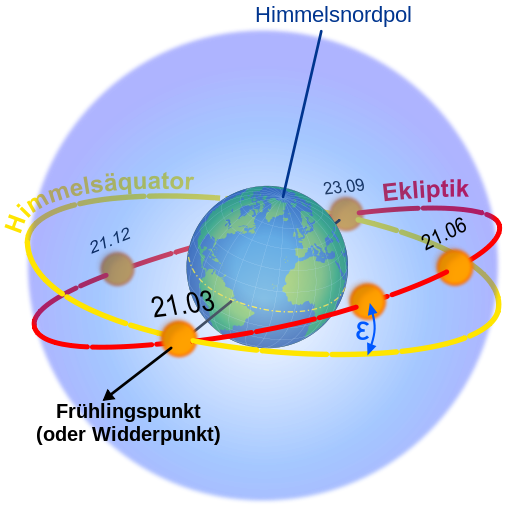
\includegraphics[scale=0.3]{./Bilder/Ecliptic.png}\hfill
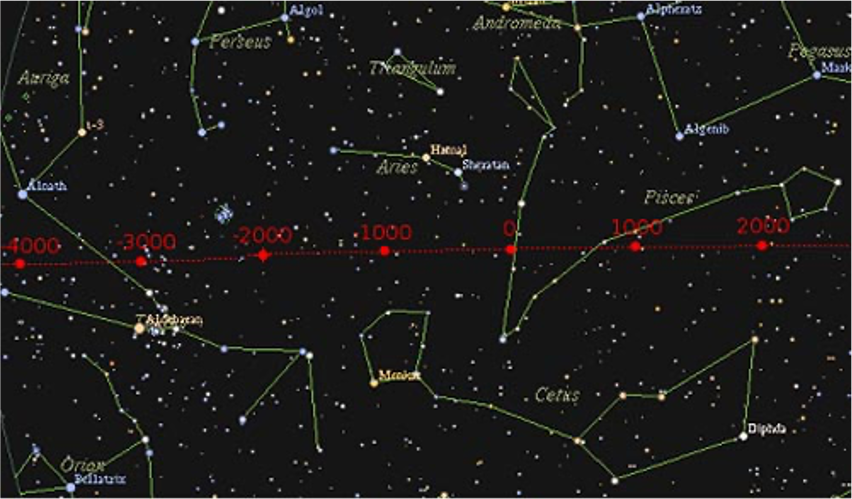
\includegraphics[scale=0.6]{./Bilder/Fr-Punkt.png}
\caption{\label{fig_Fruehlingspunkt}%
(links) Der Fr\"uhlingspunkt als der Schnittpunkt zwischen dem Himmels\"aquator und
der Ekliptik. (rechts) Der Fr\"uhlingspunkt in den letzten Jahrtausenden. W\"ahrend der 
Fr\"uhlingspunkt heute (im Jahr 2023)
im Sternbild Fische (Pisces) steht, stand er vor rund 2500 Jahren im Sternbild
Widder (Aries). Und in einigen Jahrhunderten wird er im Sternbild Wassermann stehen.
(links \cite{Wiki_Fruehling}, rechts \cite{Rocket})}
\end{figure}
 
 Die beiden Gro\ss kreise - Himmelsekliptik und Himmels\"aquator - schneiden sich in zwei
 Punkten. Der Fr\"uhlingspunkt ist definiert als der Schnittpunkt, bei dem sich die Sonne
 von S\"uden nach Norden durch die \"Aquatorialebene bewegt, beim Herbstpunkt bewegt sie sich von Nord
 nach S\"ud durch die \"Aquatorialebene. Derzeit liegt der Fr\"uhlingspunkt im Sternbild Fische. In einigen
 hundert Jahren wird er in das Sternbild Wassermann eintreten, und in babylonischer Zeit, als die Tierkreiszeichen
 benannt wurden, befand sich der Fr\"uhlingspunkt im Sternbild Widder. Aus diesem Grunde hei\ss t er 
 auch heute noch gelegentlich Widderpunkt (siehe Abb\ \ref{fig_Fruehlingspunkt}, rechts).
 
 Durch die Angabe der genannten Bezugsgr\"o\ss en - Himmelsnordpol, Himmels\"aquator und
 Fr\"uhlingspunkt auf dem Himmels\"aquator - k\"onnen wir ein Koordinatensystem f\"ur den Himmel, also
 ein sph\"arisches Koordinatensystem konstruieren.
Dazu definiert man L\"angengrade - halbe Gro\ss kreisb\"ogen vom 
 Himmelsnordpol zum Himmelss\"udpol (auch als Stundenlinien bezeichnet) -\index{Stundenlinie} 
 und Breitengrade - Kreisb\"ogen, deren Punkte unter einem konstanten
 Winkel relativ zum Himmelsnordpol stehen. Die Breitengrade werden durch die sogenannte
 Deklination\index{Deklination} 
 gekennzeichnet: Dies ist der Winkel $\delta$ von der \"Aquatorialebene zu einem Himmelsobjekt
 entlang eines L\"angengrads. Die Deklination wird als Winkel zwischen $+90^\circ$ und $-90^\circ$ 
 (Nord- bzw.\ S\"udrichtung) angegeben. Genauere Bezeichnungen verwenden meist Bogenminuten,
 Bogensekunden und dann Nachkommastellen. Der L\"angengrad wird ausgehend vom Fr\"uhlingspunkt
meist in Stundenwinkeln angegeben: der volle Himmels\"aquator wird entgegen dem Uhrzeigersinn in 
24 Stundenwinkel eingeteilt, entsprechend sind genauere Bezeichnungen in Minuten und Sekunden.
Diesen Stundenwinkel bezeichnet man als Rektazension.\index{Rektazension}
Beispielsweise hat Arkturus, einer der hellsten Sterne des Nordhimmels im Sternbild Bootes (B\"arenh\"uter), 
die Rektazension $14^{\rm h}\,15^{\rm m}\,39,67207^{\rm s}$ und die Deklination $+19^\circ\, 10'\, 56,6730''$,
bezogen auf die Epoche J2000. 

\subsection{Ekliptische Koordinaten}

Statt des Himmels\"aquators und dem dazu senkrecht stehenden Himmelsnordpol kann man 
auch\index{Ekliptische Koordinaten}\index{Koordinaten!ekliptische}
den Gro\ss kreis zur Ekliptik der Sonne und einen dazu senkrecht stehenden Punkt am Himmel
als Koordinatensystem w\"ahlen. Statt der Rektazension und der Deklination verwendet man hier den
ekliptischen L\"angengrad und den ekliptischen Breitengrad. Beide werden in Winkelma\ss en angegeben,
wobei der ekliptische L\"angengrad eine Winkeleinteilung der Ekliptik in $360^\circ$ angibt und der ekliptische
Breitengrad im Bereich zwischen $+90^\circ$ (ekliptischer Nordpol) bis $-90^\circ$ (ekliptischer S\"udpol) liegt. 
Auf der Himmelsekliptik wird ebenfalls der Fr\"uhlingspunkt als
Nullpunkt f\"ur die L\"angengrade ausgezeichnet. 

Dieses Koordinatensystem wird seltener verwendet (wegen der Bewegung vieler Planeten in der
N\"ahe der Ekliptik findet es zur Beschreibung solcher Himmelsobjekte schon mal Verwendung), sodass
wir hier nicht weiter darauf eingehen.

\subsection{Galaktische Koordinaten}

Schlie\ss lich verwendet man in der Astronomie auch gelegentlich das 
galaktische Koordinatensystem.\index{Galaktische Koordinaten}\index{Koordinaten!galaktische}
Als ausgezeichneter Referenzkreis dient ein Gro\ss kreis am Himmel, der mehr oder weniger durch
die Ebene der Milchstra\ss e, also die Sterne in der Ebene unserer Galaxie, ausgezeichnet ist. 
Der Ursprung des dreidimensionalen Koordinatensystems ist die Sonne, das Zentrum der
Galaxie (im Sternbild Sch\"utzen) dient als Referenzpunkt auf der galaktischen Ebene. 
Der galaktische Nordpol steht senkrecht auf der galaktischen Ebene und liegt im mittleren oberen Teil des Sternbilds
Haar der Berenike (Coma Berenices),\index{Haar der Berenike}\index{Coma Berenices} 
n\"ordlich des Sternbilds Jungfrau und rund $30^\circ$ s\"udlich (also
vom Nordpol weggerichtet) des Gro\ss en Wagens. 

Von der Erde aus betrachtet handelt es sich zwar um ein sph\"arisches Koordinatensystem, es
dient aber auch bei bekannten Entfernungen zu Himmelsobjekten als dreidimensionales Koordinatensystem
zur Lagebezeichnung von Objekten innerhalb unserer Galaxie.  

\section{Sternbilder}

Wie schon erw\"ahnt wurden von der IAU (International Astronomical Union) 88 Sternbilder mit ihren
Grenzen als verbindlich festgelegt (siehe Abb.\ \ref{fig_Sternbilder}).\index{Sternbild} 
Die Grenzen bestehen aus Kreisb\"ogen zu konstanter Deklination bzw.\
konstanter Rektazension - bilden somit in einer \"aquatorialen Zylinderprojektion 
senkrechte und waagerechte Linien - und umranden jeweils eine Fl\"ache.\footnote{Das Sternbild Schlange (Serpens) 
besteht als einziges Sternbild aus zwei\index{Schlange (Sternbild)}\index{Serpens caput/Serpens cauda} 
Fl\"achen, die man als Schlangenkopf (Serpens caput) und
Schlangenschwanz (Serpens cauda) bezeichnet. Die beiden Teile befinden sich rechts und links vom Sternbild 
Schlangentr\"ager (Ophiuchus)\index{Schlangentr\"ager}\index{Ophiuchus} 
und sind in den Sommermonaten am Abend in s\"udwestlicher Richtung gut zu sehen.} 
In der Summe \"uberdecken diese Fl\"achen die gesamte Himmelskugel. 

\begin{figure}[htb]
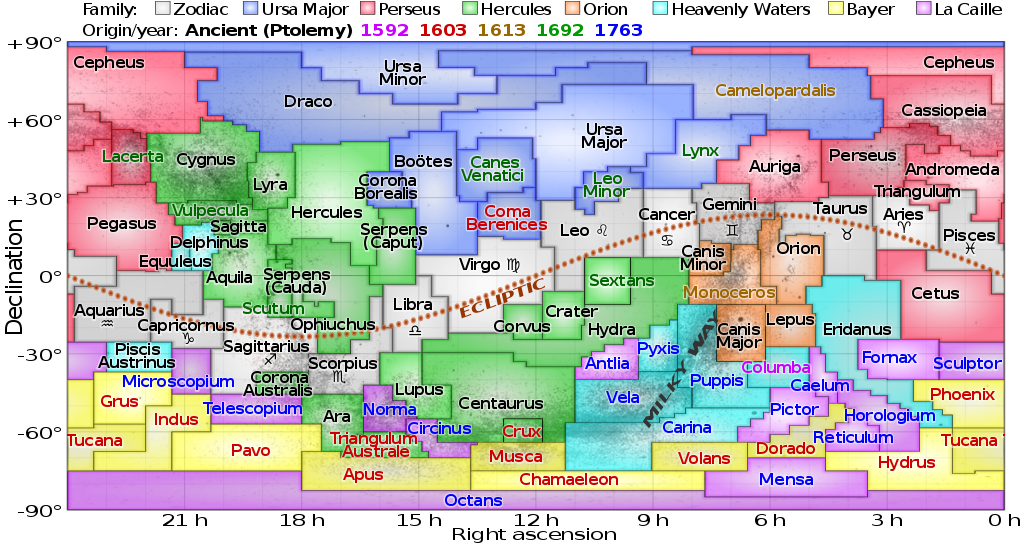
\includegraphics[scale=0.42]{./Bilder/Constellations.png}  % besser ist scale=0.42, sofern m�glich
\caption{\label{fig_Sternbilder}%
Die 88 Sternbilder in der \"Aquatorialdarstellung. Die Hintergrundfarben beziehen sich auf verschiedene Gruppen
von Sternbildern, insbesondere handelt es sich bei den grau hinterlegten Sternbildern um die klassischen
Tierkreiszeichen. In schwarzer Schrift sind die klassischen Sternbilder des Ptolem\"aus bezeichnet, andere
Farben kennzeichnen Sternbilder, die erst in sp\"aterer Zeit hinzugekommen sind. (aus \cite{Sternbilder})}
\end{figure}

In manchen Sternbildern sind mit blo\ss em Auge kaum markante Sterne zu sehen. 
Dass man diesen Fl\"achen trotzdem 
ein eigenes Sternbild zugeordnet hat liegt daran, dass man mit der Erfindung des Fernrohrs unz\"ahlige Objekte
entdeckte, die mit blo\ss em Auge nicht erkennbar sind. Um den Ort dieser Objekte am Himmel grob angeben
zu k\"onnen, hat man den gesamten Himmel mit Sternzeichen \"uberdeckt. Auf der Webseite des 
\textit{Strasbourg astronomical Data Center} \cite{IAU_Daten}
findet man die exakten Grenzen (bezogen auf das Besseljahr 1875)
aller Sternbilder. Sehr wenige Sternbilder (z.B.\ der Sextant - Sextans - 
s\"udlich vom Sternbild L\"owen) bilden\index{Sextant (Sternbild)}
ein einfaches Quadrat. Eines der komplexesten Sternbilder ist das Sternbild 
Drachen (Draco) mit rund\index{Drachen (Sternbild)}\index{Draco}
50 Grenzlinien, das sich zwischen dem kleinen und gro\ss en B\"aren halb um den Polarstern windet.   

Jedes Sternbild besitzt einen lateinischen Namen und eine Abk\"urzung mit drei Buchstaben: z.B.\ UMa f\"ur 
Ursa Major\index{Ursa Major}
 - Gro\ss e B\"arin (im Deutschen meist als Gro\ss er B\"ar bezeichnet) oder Sgr f\"ur 
 Sagittarius - Sch\"utze.\index{Sagittarius}\index{Sch\"utze (Sternbild)}
Diese Nomenklatur geht auf Henry Norris Russell zur\"uck (nach dem auch das Hertzsprung-Russell-Diagramm
benannt ist), der diese Bezeichnungen 1922 vorschlug. Innerhalb eines Sternbilds werden die hellsten Sterne
meist durch einen griechischen Buchstaben sowie den Genitiv des lateinischen Sternbildnamens 
bezeichnet, wobei sich in
der Regel die Reihenfolge $\alpha$, $\beta$, etc.\ nach der Helligkeit der Sterne richtet. Allerdings gilt diese Regel
nicht streng: Im Sternbild Ursa Major (Gro\ss er B\"ar) scheint sich die Reihenfolge eher an der Reihenfolge in
dem Asterismus Gro\ss er Wagen zu orientieren als an der Helligkeit. So ist $\alpha$ Ursae Majoris der zweithellste
Stern in diesem Sternbild, wohingegen $\epsilon$ Ursae Majoris der hellste ist. Wenn das griechische Alphabeth
durchgelaufen ist, verwendet man oft lateinische Buchstaben und anschlie\ss end Zahlen. 

Bei Doppel- oder Dreifachsternsystemen bezeichnet man die Sterne dieses Systems nach dem Namen mit einem
angeh\"angten Gro\ss buchstaben.
So ist $\alpha$ Centauri ein\index{alpha@$\alpha$ Centauri} 
Dreifachsternsystem, wobei $\alpha$ Centauri A und $\alpha$ Centauri B
vergleichsweise helle Sterne sind, wohingegen es sich bei\index{Proxima Centauri} 
$\alpha$ Centauri C (auch Proxima Centauri genannt, da
es sich mit 4,26 Lichtjahren um den uns n\"achsten Stern nach der Sonne handelt) um einen roten Zwerg handelt, der
nur in einem guten Fernrohr sichtbar ist. Oft verwendet man auch die Abk\"urzungen, beispielsweise $\alpha$ Cen A. 

Die hellsten Sterne haben eigene Namen, die meist aus der Antike stammen. Auf \cite{Wiki_hellste} findet man
eine Liste der 100 hellsten Sterne mit ihren Namen, Helligkeiten, Magnituden, offiziellen Bezeichnungen sowie
ihrer Rektazension und Deklination. Etwas umfangreichere Listen findet man auf \cite{brightest}.         

\section{Tierkreiszeichen}

Tierkreiszeichen\index{Tierkreiszeichen} 
sind Sternzeichen, die auf der Ekliptik liegen, d.h.\ vor denen von der Erde aus betrachtet 
die Sonne im Laufe eines Jahres einmal steht (siehe Abb.\ \ref{fig_Sternbilder}). 
Streng genommen sollte man zwischen den sogenannten
siderischen Tierkreiszeichen (die man besser als Sternbilder der Ekliptik bezeichnet) 
und den tropischen Tierkreiszeichen unterscheiden. 

Die siderischen Tierkreiszeichen oder auch Ekliptiksternbilder
sind die Sternzeichen, wie sie von der IAU definiert wurden und die auf der Ekliptik liegen. Sie unterteilen den
Vollkreis der Ekliptik in nicht immer exakt gleich lange Anteile von ungef\"ahr $30^\circ$. Allerdings gibt es hier schon 
eine Besonderheit: Das Sternbild des Schlangentr\"agers (Ophiuchus) \"uberdeckt zwischen dem Sternbild 
Skorpion (Scorpio) und dem Sternbild Sch\"utzen (Sagittarius) mit seinem unteren Rand ebenfalls einen 
Teil der Ekliptik. Die beiden Anteile der Ekliptik zum Skorpion und zum Schlangentr\"ager ergeben zusammen
einen Abschnitt von ungef\"ahr $30^\circ$, wobei der Anteil des Schlangentr\"agers deutlich gr\"o\ss er als der des
Skorpions ist. Der Schlangentr\"ager z\"ahlt aber in der Tradition nicht zu den Tierkreiszeichen. In manchen Listen
wird der Schlangengtr\"ager heute als 13.\ Tierkreiszeichen hinzugez\"ahlt, insbesondere wenn man von den
siderischen Tierkreiszeichen bzw.\ Ekliptiksternbildern spricht. 

Dem gegen\"uber gibt es die tropischen Tierkreiszeichen. Sie unterteilen die Ekliptik in zw\"olf exakt gleich gro\ss e
Anteile von $30^\circ$ und tragen dieselben Bezeichnungen wie die siderischen Tierkreissternbilder. 
Allerdings hat sich aufgrund der Pr\"azission der Erde der Fr\"uhjahrspunkt im Verlauf der Zeit verschoben. Vor etwas
\"uber 2500 Jahren, als die Bezeichnungen der Tierkreiszeichen in Babylonien entstanden sind, 
befand sich der Fr\"uhjahrspunkt im
Sternbild Widder, weshalb man ihn auch heute noch manchmal als Widderpunkt bezeichnet. Auf diese Einteilung
der Ekliptik in zw\"olf gleiche Teile bezieht sich auch heute noch die Astrologie: Die astrologischen Tierkreiszeichen 
beginnen am 21.\ M\"arz mit dem Zeichen Widder und schreiten in nahezu gleichen zeitlichen Abst\"anden um jeweils
$30^\circ$ voran.\footnote{Die Wendepunkte und \"Aquinoktien definieren jeweils gleiche Abschnitte von $90^\circ$.
Wegen der elliptischen Bahn und der damit verbundenen ungleichen Geschwindigkeit der Erde um die Sonne 
sind die zugeh\"origen r\"aumlichen und zeitlichen Abschnitte jedoch nicht
exakt gleich lang.} Heute liegt der Fr\"uhjahrspunkt im Sternbild Fische, und in einigen Jahrhunderten wird er
ins Sternbild Wassermann gewandert sein. Das bedeutet, derzeit sind die tropischen und die 
siderischen Tierkreiszeichen gegeneinander um ein Zeichen verschoben: Am 21.\ M\"arz, 
wenn das tropische Tierkreiszeichen Widder
beginnt, befindet sich die Sonne im Sternzeichen Fische.  

Unter dem Zodiak,\index{Zodiak} 
fr\"uher oft synonym zu Tierkreiszeichen verwendet, versteht man heute ein Band von rund 
$\pm 10$ Grad um die Ekliptik, in der sich die meisten Planetenbahnen sowie die Bahn des Mondes bewegen. Auch 
der Zodiak ist in zw\"olf exakt $30^\circ$ umfassende Bereiche unterteilt und richtet sich insofern nach den
tropischen Tierkreiszeichen. 

Gew\"ohnlich beginnt man die Reihe der Tierkreiszeichen mit dem\index{Widder (Sternbild)}\index{Aries} 
Widder (Aries), in dem vor rund 2500 Jahren der 
Fr\"uhlingspunkt lag. In aufsteigender Rektazension, also entgegen dem Uhrzeigersinn, folgen die Tierkreiszeichen
Stier (Taurus), Zwillinge (Gemini), Krebs (Cancer), L\"owe (Leo), Jungfrau (Virgo), Waage (Libra), Skorpion (Scorpius),
Sch\"utze (Sagittarius), Steinbock (Capricornus), Wassermann (Aquarius) und Fische (Pisces), wobei man 
im Zusammenhang mit den Ekliptiksternbildern 
zwischen den Skorpion und den Sch\"utzen noch den Schlangentr\"ager als 13.\ Tierkreissternbild einf\"ugt. 

\section{Asterismen}

Asterismen\index{Asterismus} 
sind einzelne Gruppen von Sternen, die ein markantes Muster zeigen. Bekannte
Beispiele sind der gro\ss e und kleine Wagen in den Sternbildern Ursa Major und Ursa Minor mit jeweils
sieben Sternen, wobei man bei nicht optimalen Sichtverh\"altnissen vom kleinen Wagen oft nur drei
Sterne sieht, oder auch das Himmels-W der Kassiopeia aus f\"unf Sternen. Ein weiteres Beispiel
(bekannt unter anderem aus dem Film \glqq Men in Black\grqq) ist der G\"urtel des Orion, bestehend
aus drei hellen Sternen in einer Reihe. 

Ein Asterismus kann auch aus Sternen zu verschiedenen Sternbildern bestehen. Beispiele
hier sind das Fr\"ulingsdreieck,\index{Fruehlingsdreieck@Fr\"uhlingsdreieck} 
bestehend aus Spica (Sternbild Jungfrau - Virgo), Arktur (Sternbild 
B\"arenh\"uter - Bootes) und Regulus (Sternbild L\"owe - Leo), oder auch das 
Sommerdreieck,\index{Sommerdreieck}
bestehend aus Wega (Sternbild Leier - Lyra), Altair (Sternbild Adler - Aquila) und Deneb (Sternbild Schwan - Cygnus). 
Hierbei handelt es sich jeweils um eine Gruppe von drei besonders hellen Sternen, die man im
Fr\"uhjahr bzw.\ im Sommer am Abendhimmel sehen kann. Ein weiteres Beispiel ist das 
Wintersechseck,\index{Wintersechseck}
bestehend aus den Sternen Capella (Sternbild Fuhrmann - Auriga), Aldebaran (Sternbild Stier - Taurus), 
Rigel (Sternbild Orion), Sirius (Sternbild Gro\ss er Hund - Canis Major), Prokyon (Sternbild Kleiner Hund -
Canis Minor) und Pollux (Sternbild Zwillinge - Gemini). Diese Sterngruppen erstrecken sich teilweise
\"uber einen gro\ss en Teil des Nachthimmels. 

Es gibt aber auch sehr kleine Asterismen, die man mit blo\ss em Auge kaum aufl\"osen kann, wohl
aber mit einem einfachen Fernglas: Ein Beispiel ist der\index{Kleiderb\"ugel (Asterismus)} 
\glqq Kleiderb\"ugel\grqq\ im Sternbild Fuchs (Vulpecula,
zwischen den Sternbildern Adler und Schwan gelegen). Der Asterismus besteht aus 10 Sternen, von denen
sechs nahezu auf einer Geraden liegen, plus vier Sterne, die in der Mitte \"uber dieser Geraden einen
Dreiviertelkreis bilden. Insgesamt erscheint diese Konfiguration, die offiziell den 
Namen Collinder 399 tr\"agt,\index{Collinder 399}
wie ein Kleiderb\"ugel.   


\begin{thebibliography}{99}
\bibitem{IAU_Daten} Strasbourg astronomical Data Center, Grenzen der Sternbilder:\\
      \url{https://vizier.cds.unistra.fr/vizier/VizieR/constellations.htx}.   
\bibitem{Rocket} Rocket Site \glqq Wann beginnt das Zeitalter des Wassermanns?\grqq\
               \url{https://damthoitrang.org/de/wann-beginnt-das-zeitalter-des-wassermanns/}      
\bibitem{Sternbilder} aus Wikipedia \glqq Zodiac\grqq, Quelle: 
%https://upload.wikimedia.org/wikipedia/commons/8/89/Constellations%2C_equirectangular_plot%2C_Menzel_families.svg
      \url{http://svs.gsfc.nasa.gov/vis/a000000/a003500/003572}, Autor: Cmglee, Timwi, NASA. 
\bibitem{Wiki_Fruehling} Wikipedia \glqq \"Aquinoktium\grqq, 
                 \url{https://commons.wikimedia.org/wiki/File:Ecliptic.svg}
\bibitem{Wiki_hellste} Wikipedia \glqq Liste der hellsten Sterne\grqq: 
      \url{https://de.wikipedia.org/wiki/Liste_der_hellsten_Sterne} 
\bibitem{brightest} Listen heller Sterne: \url{http://stars.astro.illinois.edu/sow/bright.html} (Webseite von
      Jim Kahler, die 172 hellsten Sterne) und
       \url{http://www.atlasoftheuniverse.com/stars.html} (Atlas of the Universe; die 300 hellsten Sterne). 
\end{thebibliography}

\end{document}


%\documentclass[german,10pt]{book}      
\usepackage{makeidx}
\usepackage{babel}            % Sprachunterstuetzung
\usepackage{amsmath}          % AMS "Grundpaket"
\usepackage{amssymb,amsfonts,amsthm,amscd} 
\usepackage{mathrsfs}
\usepackage{rotating}
\usepackage{sidecap}
\usepackage{graphicx}
\usepackage{color}
\usepackage{fancybox}
\usepackage{tikz}
\usetikzlibrary{arrows,snakes,backgrounds}
\usepackage{hyperref}
\hypersetup{colorlinks=true,
                    linkcolor=blue,
                    filecolor=magenta,
                    urlcolor=cyan,
                    pdftitle={Overleaf Example},
                    pdfpagemode=FullScreen,}
%\newcommand{\hyperref}[1]{\ref{#1}}
%
\definecolor{Gray}{gray}{0.80}
\DeclareMathSymbol{,}{\mathord}{letters}{"3B}
%
\newcounter{num}
\renewcommand{\thenum}{\arabic{num}}
\newenvironment{anmerkungen}
   {\begin{list}{(\thenum)}{%
   \usecounter{num}%
   \leftmargin0pt
   \itemindent5pt
   \topsep0pt
   \labelwidth0pt}%
   }{\end{list}}
%
\renewcommand{\arraystretch}{1.15}                % in Formeln und Tabellen   
\renewcommand{\baselinestretch}{1.15}                 % 1.15 facher
                                                      % Zeilenabst.
\newcommand{\Anmerkung}[1]{{\begin{footnotesize}#1 \end{footnotesize}}\\[0.2cm]}
\newcommand{\comment}[1]{}
\setlength{\parindent}{0em}           % Nicht einruecken am Anfang der Zeile 

\setlength{\textwidth}{15.4cm}
\setlength{\textheight}{23.0cm}
\setlength{\oddsidemargin}{1.0mm} 
\setlength{\evensidemargin}{-6.5mm}
\setlength{\topmargin}{-10mm} 
\setlength{\headheight}{0mm}
\newcommand{\identity}{{\bf 1}}
%
\newcommand{\vs}{\vspace{0.3cm}}
\newcommand{\noi}{\noindent}
\newcommand{\leer}{}

\newcommand{\engl}[1]{[\textit{#1}]}
\parindent 1.2cm
\sloppy

         \begin{document}  \setcounter{chapter}{8}


\chapter{Die Kosmische Entfernungsleiter}
% Kap 9
\label{chap_Kosm_Entfernung}

\info{Thomas Filk}{28.03.2024}%
Die Bestimmung astronomischer bzw.\ kosmischer Entfernungen ist sowohl ein
spannendes Thema der Geschichte der Physik als auch ein interessantes
Forschungsfeld der modernen Physik. W\"ahrend der Abstand von der Erde zum
Mond schon im Altertum bekannt war (siehe Abschnitte \ref{sec_Aristarchos} und \ref{sec_Eratosthenes}) 
kennt man den Abstand von der Erde zur Sonne -- die sogenannte Astronomische
Einheit AU (astronomical unit) -- mit einer gewissen Verl\"asslichkeit erst seit dem 18.\ Jahrhundert.

Tabelle \ref{tab_Arist} enth\"alt einige Daten, die in diesem Abschnitt gelegentlich
verwendet werden.\index{Abstand!Erde-Sonne}\index{Abstand!Erde-Mond}\index{AU - Astronomische Einheit}%
\index{Erddurchmesser}\index{Monddurchmesser}\index{Sonne!Durchmesser}

\begin{table}[htb]
\begin{tabular}{l|c|l}
Bezeichnung & Symbol & Wert \\ \hline
Durchmesser Erde & $D_{\rm E}$ &  $D_{\rm E}= 12\,740\,{\rm km}$ \\
Durchmesser Mond & $D_{\rm M}$ &  $D_{\rm M}= 3\,474\,{\rm km}$ \\
Durchmesser Sonne & $D_{\rm S}$ &  $D_{\rm S}=  1\,400\,000 \,{\rm km}$ \\
Abstand Erde-Mond & $r_{\rm M}$  &  $r_{\rm M} = 380\,000\,{\rm km}$ \\
Abstand Erde-Sonne & $r_{\rm S}$  &  $r_{\rm S} = 150\,000\,000\,{\rm km}$ \\
Winkel Sonne-Mond bei Halbmond & $\alpha$ & $\alpha = 89^\circ 51'$ \\ \hline
\end{tabular}
\caption{\label{tab_Arist}%
Einige Daten des Sonne-Erde-Mond-Systems.}
\end{table}

\section{Aristarchos von Samos}
\label{sec_Aristarchos}

Aristarchos von Samos\index{Aristarchos von Samos} 
lebte um 310\,v.Chr. bis 230\,v.Chr, also kurz nach Aristoteles (384-322 v.Chr.)
und ungef\"ahr zeitgleich mit Archimedes (284-212\,v.Chr.). Er stellte sich die Sonne als ein riesiges
Himmelsfeuer vor, das unter anderem den Mond anstrahlt. Er deutete eine Mondfinsternis
korrekt als ein Ereignis, bei dem sich die Erde zwischen Sonne und Mond schiebt und dadurch
auf dem Mond der Erdschatten sichtbar wird. Au\ss erdem deutete er den Halbmond als das Ereignis,
bei dem die Verbindungslinie Sonne-Mond senkrecht zur Verbindungslinie Erde-Mond steht. Aus diesen
beiden Interpretationen sowie den zugeh\"origen Messungen konnte er \textit{relative} Gr\"o\ss en
bestimmen: das Verh\"altnis der Abst\"ande Erde-Mond zu Erde-Sonne, das Verh\"altnis Monddurchmesser zu
Sonnendurchmesser, das Verh\"altnis Monddurchmesser zu Erddurchmesser und schlie\ss lich
konnte er daraus das Verh\"altnis der Gr\"o\ss e der Sonne zur Gr\"o\ss e der Erde bestimmen. Seine
Schlussfolgerung war, dass die Sonne wesentlich gr\"o\ss er sein muss als die Erde, und damit sollte
seiner Meinung nach die Sonne im Zentrum des Universums stehen. Dadurch wurde er einer der ersten
Vertreter eines heliozentrischen Weltbilds.

\begin{figure}[htb]
\begin{tikzpicture}
\draw (1,1.5) circle (1.6cm);
\draw (9.3,1.5) circle (0.15cm);
\draw (10.6,1.5) circle (0.4cm);
\draw (1,-0.1) -- (10.2,1.5);
\draw (1,3.1) -- (10.2,1.5);
\draw (1,-0.1) -- (14,1.5);
\draw (1,3.1) -- (14,1.5);
\filldraw[fill=gray!20] (14,1.5) -- (10.6,1.1) arc (270:440:0.4cm) -- (14,1.5);
\draw (11.9,1.5) circle (0.15cm);
\draw (11.83,1.07) circle (0.15cm);
\draw (1,-0.1) -- (1,3.1);
\draw (1.3,1.5) node{$D_{\rm S}$}; 
\draw (10.6,1.1) -- (10.6,1.9);
\draw (10.8,1.5) node{${\scriptstyle D_{\rm E}}$}; 
\draw (8.7,1.5) node{\footnotesize Mond}; 
\draw (1,-0.5) -- (10.6,-0.5);
\draw (1,-0.6) -- (1,-0.4);
\draw (10.6,-0.6) -- (10.6,-0.4);
\draw (6.3,-0.27) node{$r_{\rm S}$}; 
\draw (9.3,0.0) -- (10.6,0.0);
\draw (9.3,-0.1) -- (9.3,0.1);
\draw (10.6,-0.1) -- (10.6,0.1);
\draw (9.8,0.18) node{$r_{\rm M}$}; 
\draw (10.6,-0.25) -- (14.0,-0.25);
\draw (10.6,-0.35) -- (10.6,-0.15);
\draw (14,-0.35) -- (14,-0.15);
\draw (12.3,-0.05) node{$R$}; 
\draw (14.2,1.245) -- (14.2,1.755);
\draw (14.1,1.245) -- (14.3,1.245);
\draw (14.1,1.755) -- (14.3,1.755);
\draw (14.4,1.5) node{$B$}; 
\filldraw[fill=black!100] (11.88,1.755) circle (0.03cm);
\filldraw[fill=black!100] (11.88,1.245) circle (0.03cm);
\draw (10.6,1.5) circle (1.3cm);
\draw (9.6,1.75) node{\tiny (1)}; 
\draw (12.17,1.05) node{\tiny (2)}; 
\draw (12.25,1.5) node{\tiny (3)}; 
\end{tikzpicture}
\caption{\label{fig_Arist}%
Nicht ma\ss stabsgetreue Verh\"altnisse zwischen Sonne, Mond und Erde. Es sind drei
Mondphasen dargestellt: (1) Der Mond bei einer Sonnenfinsternis, er erscheint genauso gro\ss\ wie die
Sonne; (2) der Mond tritt in den Erdschatten und (3) der Mond befindet sich
im Erdschatten. $R$ bezeichnet die L\"ange des Erdschattens und $B$ seine Breite an der Stelle
des Monddurchgangs.}
\end{figure}

In vereinfachten Rechnungen nimmt man gelegentlich an, dass der Erdschatten beim Mond denselben Durchmesser
hat wie die Erde. Das setzt voraus, dass die Sonne \glqq unendlich\grqq\ weit entfernt ist, sodass der 
Erdschatten durch nahezu paralleles Sonnenlicht entsteht. Diese Annahme konnte Aristarchos aber 
nicht machen: Erstens wollte er ja erst zeigen, dass die Sonne sehr weit von der Erde entfernt ist,
und zweitens war der relative Abstand, den er aus seinen Messungen erhielt, um einen Faktor 20
kleiner als in Wirklichkeit. Au\ss erdem steht eine solche Annahme in einem (etwas versteckten) Widerspruch 
zu einer in die Rechnungen eingehenden Beobachtung und f\"uhrt zu
einem deutlichen Fehler, wie gegen Ende dieses Abschnitts gezeigt wird. 

Statt dessen nahm Aristarchos an, dass sich der Erdschatten hinter der Erde wie ein Kegel
verj\"ungt und daher der Mond bei einer Mondfinsternis einen kleineren Schattendurchmesser 
durchl\"auft, als es dem Erddurchmesser entspricht (siehe Abb.\ \ref{fig_Arist}). Um diese 
Verj\"ungung des Erdschattens ber\"ucksichtigen 
zu k\"onnen, musste er erst bestimmen, wie weit die Sonne von der Erde relativ zum Mond entfernt ist.

\begin{figure}[htb]
\begin{tikzpicture}
\draw (1,1.5) circle (1.0cm);
\draw (10.5,2.8) circle (0.15cm);
\draw (10.6,1.5) circle (0.4cm);
\draw (1,1.5) -- (10.5,2.8) -- (10.6,1.5) -- (1,1.5);
\draw (10.6,1.4) node{\footnotesize Erde}; 
\draw (11.1,2.8) node{\footnotesize Mond}; 
\draw (1,1.4) node{\footnotesize Sonne}; 
\draw (10.45,1.65) node{${\scriptstyle \alpha}$};
\filldraw[fill=black!100] (10.35,2.55) circle (0.03cm);
\draw (10,2.75) arc (185:275:0.5cm);
\draw (6,1.3) node{$r_{\rm S}$};
\draw (10.85,2.15) node{$r_{\rm M}$};
\filldraw[fill=gray!50] (10.52,2.65) arc (278:458:0.15cm);
\end{tikzpicture}
\caption{\label{fig_Arist2}%
Der Mond bei Halbmond. Der Winkel, unter dem vom Mond aus betrachtet die Zentren von
Sonne und Erde erscheinen, betr\"agt $90^\circ$. Der Winkel, unter dem von der Erde
aus betrachtet die Zentren von Sonne und Mond erscheinen ist $\alpha$. Der Kosinus von $\alpha$ entspricht 
dem Verh\"altnis von den Abst\"anden Erde-Mond zu Erde-Sonne.}
\end{figure}

F\"ur die Bestimmung der relativen Entfernung der Sonne ging Aristarchos von folgender 
\"Uberlegung aus: Bei Halbmond ist der Winkel zwischen der Verbindungslinie Sonne-Mond
und der Verbindungslinie Erde-Mond ein rechter Winkel (siehe Abb.\ \ref{fig_Arist2}). Wenn man nun hier auf der
Erde den Winkel $\alpha$ zwischen den Verbindungslinien Erde-Sonne und Erde-Mond 
bestimmt, erh\"alt man das Verh\"altnis der Abst\"ande von Erde-Sonne zu Erde-Mond.
Heute w\"urden wir daf\"ur schreiben:
\begin{equation}
\label{eq_Arist1}
                     \frac{r_{\rm M}}{r_{\rm S}} = \cos \alpha \, . 
\end{equation} 
Allerdings erhielt Aristarchos f\"ur diesen Winkel mit $\alpha = 87^\circ$ einen viel zu kleinen Wert.
Der tats\"achliche Wert ist $89^\circ 51'$. Vermutlich war sich Aristarchos dar\"uber im Klaren, dass
der Wert f\"ur $\alpha$ kleiner als $90^\circ$ sein muss und sein Wert ist eher als eine
untere Grenze zu verstehen. 
Mit dem Wert von Aristarchos ist der Abstand Sonne-Erde
rund 19 mal gr\"o\ss er als der Abstand Erde-Mond. In Wirklichkeit ist das Verh\"altnis knapp 400. 
Da die Sonne von der Erde aus betrachtet \"ahnlich gro\ss\ erscheint wie der Mond (bei einer
Sonnenfinsternis wird die Sonne vom Mond gerade eben bedeckt), ist die Sonne um dasselbe
Verh\"altnis gr\"o\ss er als der Mond - f\"ur Aristarchos rund 19 mal gr\"o\ss er. Das bedeutet:
\begin{equation}
\label{eq_Arist2}
                           \frac{D_{\rm S}}{D_{\rm M}} = \frac{r_{\rm S}}{r_{\rm M}} \, .
\end{equation}

Aus Abbildung \ref{fig_Arist} erhalten wir die folgenden geometrischen Beziehungen (in beiden F\"allen
aus dem Strahlensatz):
\begin{equation}
\label{eq_Arist3}
        \frac{D_{\rm S}}{D_{\rm E}} = \frac{R+r_{\rm S}}{R} =  1+\frac{r_{\rm S}}{R}  \hspace{1.0cm} {\rm und} \hspace{1cm}
        \frac{B}{D_{\rm E}} = \frac{R-r_{\rm M}}{R} =  1-\frac{r_{\rm M}}{R}  \, .
\end{equation}
Eine weitere Beziehung erhielt Aristarchos aus der Messung von zwei Zeitdauern: 
$t_1$ sei die Zeitdauer zwischen dem Moment, in dem der Mond in den Schatten der Erde eintritt, bis
zu dem Moment, wo er sich ganz im Erdschatten befindet, und $t_2$ sei die Zeitdauer, in der sich der Mond 
vollst\"andig im Erdschatten befindet. 
Das Verh\"altnis dieser beiden Zeiten ist
\begin{equation}
\label{eq_Arist4}
           \frac{t_1}{t_2} = \frac{D_{\rm M}}{B-D_{\rm M}}   \hspace{1.0cm} {\rm oder} \hspace{1.0cm}
             B= \frac{t_1+t_2}{t_1} D_{\rm M} \, .
\end{equation}
Aus den beiden Beziehungen in Gl.\ \ref{eq_Arist3} k\"onnen wir die L\"ange $R$ des Erdschattens eliminieren,
die Breite $B$ des Erdschattens bei der Mondbahn k\"onnen wir durch Gl.\ \ref{eq_Arist4} ersetzen und
schlie\ss lich k\"onnen wir noch den Sonnendurchmesser $D_{\rm S}$ mit Hilfe von Gl.\ \ref{eq_Arist2} 
durch den Monddurchmesser $D_{\rm M}$ und das bekannte Verh\"altnis $\frac{r_{\rm S}}{r_{\rm M}}$ ersetzen.
Nach einer etwas l\"angeren Rechnung erhalten wir dann:
\begin{equation}
\label{eq_Arist5}
             \frac{D_{\rm E}}{D_{\rm M}} 
             = \frac{\displaystyle \left( 1 + \frac{t_1+t_2}{t_1} \right)}{\displaystyle 1 + \frac{r_{\rm M}}{r_{\rm S}}} \, .
\end{equation}
Auf der rechten Seite stehen nur Gr\"o\ss en, die Aristarchos gemessen hatte. 
Aus seinen Beobachtungen schloss er,
dass die Erde ungef\"ahr 3 mal gr\"o\ss er ist als der Mond (sein Wert war 2,85, der wirkliche Wert
ist 3,67). Zusammen mit seinem Faktor 19 zwischen der Gr\"o\ss e des Monds und der
Gr\"o\ss e der Sonne erhielt er somit, dass die Sonne rund $6,7$ mal gr\"o\ss er sein muss als die
Erde. Der wirkliche Faktor ist knapp 110. 

\begin{SCfigure}[30][htb]
\begin{tikzpicture}
\draw (0,0) node{\mbox{~}};
\draw (8.5,0) node{\mbox{~}};
\draw (2.5,1) node{${\scriptstyle \theta}$};
\draw (8.3,1) node{${\scriptstyle D_{\rm M}}$};
\draw (5,0.85) node{${\scriptstyle r_{\rm M}}$};
\draw (0.2,1) -- (2.3,1);
\draw (2.7,1) -- (8,1);
\draw (0.2,1) -- (8,0.5) -- (8,1.5) -- (0.2,1) ;
\draw[thick] (8.02,0.5) -- (8.02,1.5);
\draw (2.6,0.84) arc (351:369:1.0); 
\end{tikzpicture}
\caption{\label{fig_Arist3}%
Aus dem \"Offnungswinkel, unter dem der Mond von der Erde aus gesehen wird (ungef\"ahr $30'$) kann man auf
das Verh\"altnis von Monddurchmesser $D_{\rm M}$ zum Abstand Erde-Mond $r_{\rm M}$ schlie\ss en.}
\end{SCfigure}

Dar\"uber hinaus konnte Aristarchos
aus der scheinbaren Gr\"o\ss e des Monds (ungef\"ahr $0,5^\circ$ \"Offnungswinkel) das
Verh\"altnis von der Gr\"o\ss e des Monds $D_{\rm M}$ zu seinem Abstand $r_{\rm M}$ 
von der Erde bestimmen (siehe Abb.\ \ref{fig_Arist3}).
Die Beziehung ist:
\begin{equation}
\label{eq_Parallaxe}
                       \tan \frac{\theta}{2} = \frac{D_{\rm M}}{2 r_{\rm M}} \, .
\end{equation}  

H\"atten wir f\"ur die Breite $B$ des Erdschattens beim Mond einfach den Erddurchmesser
angenommen, h\"atten wir direkt aus Gl.\ \ref{eq_Arist4} die Beziehung
\begin{equation}
                  \frac{D_{\rm E}}{D_{\rm M}}  = \frac{t_1+t_2}{t_1}    
\end{equation}  
erhalten. Doch
dieses Ergebnis folgt nicht, wenn wir in Gl.\ \ref{eq_Arist5} den Grenzfall $r_{\rm S} \rightarrow \infty$ 
nehmen. Immerhin ist in Wirklichkeit das Verh\"altnis $r_{\rm M}/r_{\rm S}\approx 1/400$ und somit in guter
N\"aherung vernachl\"assigbar. Der zus\"atzliche Term \glqq $1+$\grqq\ im Z\"ahler von Gl.\ \ref{eq_Arist5} r\"uhrt 
ebenfalls daher, dass wir einen kegelartigen Schatten angenommen haben, der an der Stelle des Monds schon 
deutlich kleiner ist als der Erddurchmesser. Wenn $r_{\rm S}$ im Vergleich zu $r_{\rm M}$ gro\ss\ wird, muss
wegen Gl.\ \ref{eq_Arist2}, die wir bei der Herleitung von Gl.\ \ref{eq_Arist5} verwendet haben, auch der
Sonnendurchmesser im selben Verh\"altnis zunehmen. Das bedeutet aber, dass die Schattenl\"ange
$R$ nahezu konstant bleibt (die Korrektur hierzu wird durch den Nenner von Gl.\ \ref{eq_Arist5} beschrieben)
und damit auch das Verh\"altnis, um das der Erdschatten beim Mond kleiner ist. F\"ur das Erde-Sonne-Mond-System
ist $R$ ungef\"ahr das Vierfache von $r_{\rm M}$, und damit ist der Erdschatten beim Mondabstand schon
um ungef\"ahr den Faktor 3:4 kleiner als der Erddurchmesser.  

\section{Eratosthenes von Kyrene}
\label{sec_Eratosthenes}

Wie wir gesehen haben, hat Aristarchos nur Verh\"altnisse von Gr\"o\ss en bestimmt, keine
absoluten Werte. Dazu muss mindestens eine der Gr\"o\ss en bekannt sein. 
Dieses\index{Eratosthenes von Kyrene}
Problem l\"oste Eratosthenes von Kyrene, der kurz nach Aristarchos lebte. Seine genauen
Lebensdaten sind nicht bekannt, aber bis auf ein oder zwei Jahre lebte er von 276\,v.Chr.\ bis
194\,v.Chr. Bekannt ist Eratosthenes unter anderem durch das gleichnamige \glqq Sieb\grqq, mit dem man 
eine Tabelle der Primzahlen erh\"alt. 

Eratosthenes wusste, dass es in der N\"ahe von Assuan (damals Syene) einen tiefen Brunnen
gab, bei dem die Sonne nur einmal im Jahr -- am 21.\ Juni zur Mittagszeit 
(d.h.\ bei Sonnenh\"ochststand) -- den Boden beleuchtete. Er deutete dies 
als die Tatsache, dass an diesem Tag die Sonne senkrecht \"uber Assuan steht. Assuan liegt am
24.\ Breitengrad und somit nur wenig \"uber dem Sommerwendekreis der Sonne (bei $23,5^\circ$). 
Weiterhin nahm Eratosthenes an, dass die Stadt Alexandria auf demselben L\"angengrad wie
Assuan liegt, was nicht ganz richtig ist: Alexandria liegt rund $3^\circ$ weiter westlich. Dieser
Winkel ist jedoch klein genug, um in die
folgenden \"Uberlegungen nur unwesentlich einzugehen. 
Schlie\ss lich wusste Eratosthenes noch, dass der Schatten eines Obelisken in Alexandria zur
Mittagszeit des 21.\ Juni unter einem Winkel von $1/50$.tel eines Vollkreises (also $\theta=7,2^\circ$) fiel. 
Aus der Annahme, dass die Sonnenstrahlen parallel einfallen, konnte er daraus 
schlie\ss en, dass der Erdumfang das 50-fache des Abstands von Alexandria nach Syene 
betr\"agt. 

\begin{SCfigure}[30][htb]
\begin{tikzpicture}
\draw (0,0) node{\mbox{~}};
\filldraw[fill=black!100] (0.5,1.4) circle (0.05cm);
%\draw (0.5,1.4) circle (2cm);
\draw (1.92,0) arc (315:358:2);
\draw (2.5,1.45) arc (363:420:2);
\draw (2.5,1.45) -- (2,1.45) -- (2,1.35) -- (2.5,1.35);
\draw (2.34,2.1) -- (2.82,2.3) -- (2.79,2.35) -- (2.31,2.16);
\draw (0.5,1.4) -- (2.0,1.4);
\draw (2.79,2.35) -- (2.21,2.35);
\draw (2.21,2.35) -- (0.5,1.4);
\filldraw[fill=gray!30] (2.21,2.35) -- (2.33,2.16) -- (2.79,2.35) -- (2.21,2.35);
\draw[->] (8,1.4) -- (4,1.4);
\draw[->] (8,2.3) -- (4,2.3);
\draw (2.7,2.7) node{${\scriptstyle \theta}$};
\draw (1.1,1.4) arc (0:26:0.7);
\draw[->]  (2.6,2.6) arc (160:193:0.5);
\draw (0.9,1.5) node{${\scriptstyle \theta}$};
\draw (2.65,1.2) node{\footnotesize S};
\draw (2.2,2.0) node{\footnotesize A};
\draw (7,1.85) node{\footnotesize Sonne};
\end{tikzpicture}
\caption{\label{fig_Erat}%
Zur Bestimmung des Erdumfangs nach Eratosthenes. Am 21.\ Juni steht die Sonne
mittags senkrecht \"uber einem Brunnen in Syene (S). Zum gleichen Zeitpunkt wirft ein
Obelisk in Alexandria (A) einen Schatten unter dem Winkel $\theta$. Unter demselben
Winkel erscheinen Syene und Alexandria vom Erdmittelpunkt aus betrachtet.}
\end{SCfigure}  

Wie er den Abstand zwischen Alexandria und Syene bestimmt hat, ist nicht genau bekannt. Es gilt aber als wahrscheinlich,
dass er k\"onigliche Schrittz\"ahler eingesetzt hat, diesen Abstand zu messen. Das Ergebnis
waren 5000 Stadien. Es ist auch nicht bekannt, welche Einheit f\"ur ein Stadion Eratosthenes
verwendet hat (es waren damals mehrere Einheiten gebr\"auchlich), vermutlich aber handelte
es sich um eine Einheit nahe bei 160\,m.\footnote{Das mesopotamische Stadion betrug 148,5\,m, das
griechische 177,6\,m. In manchen griechischen Schriften findet man auch 157,5\,m.} 
In diesem Fall h\"atte er die Entfernung Alexandria-Syene 
nach heutigen Einheiten zu 800\,km bestimmt. Da dies 1/50.\ des Erdumfangs entsprechen
soll, bestimmte er den Erdumfang zu 40\,000\,km. Wie genau diese Werte mit seinen Werten
\"ubereinstimmen, ist nicht bekannt, aber immerhin handelte es sich um ein wissenschaftliches
Verfahren, wohingegen viele andere Werte f\"ur die Gr\"o\ss e der Erde auf reinen Vermutungen beruhten. 

\section{Die Gr\"o\ss e der Erde}

Bis in die fr\"uhe Neuzeit wurden die antiken Ergebnisse zur Bestimmung der Gr\"o\ss e
der Erde oder des Abstands Erde-Sonne kaum \"ubertroffen. Die Zahlen von Eratosthenes
blieben obskur, solange nicht gekl\"art war, was genau unter einem Stadion zu verstehen war.
Doch die allgemeine Idee zur Bestimmung der Gr\"o\ss e der Erde war korrekt. 

Zu Beginn des 17.\ Jahrhunderts gab es zwei Entdeckungen, die einen wesentlichen
Fortschritt brachten: (1) die Erfindung des Fernrohrs um 1610 und (2) die Kepler'schen Gesetze,
insbesondere das dritte Kepler'sche Gesetz, das eine Beziehung zwischen den gro\ss en Halbachsen
und den Umlaufzeiten eines Planeten um die Sonne herstellte (ver\"offentlicht 1619). 

Mit Hilfe des Fernrohrs konnte die Erdgr\"o\ss e wesentlich genauer bestimmt werden. Hier ist
insbesondere\index{Picard, Jean} 
Jean Picard (1620--1682) zu erw\"ahnen, der um 1670 eine sehr genaue Vermessung
des Erdradius vornahm. Voraussetzung daf\"ur waren (1) die Festlegung von zwei 
m\"oglichst weit voneinander entfernten Orten auf demselben L\"angengrad, (2) eine 
m\"oglichst genaue Bestimmung der Entfernung zwischen diesen beiden Orten und (3) eine
m\"oglichst genaue Messung der Breitengrade dieser Orte. Picard verwendete zur Winkelmessung
zwischen zwei Orten Quadranten, die mit kleinen Fernrohren mit Fadenkreuzen ausgestattet
waren. Dadurch waren sehr pr\"azise Winkelmessungen m\"oglich. Diese verwendete er einerseits,
um den Breitengrad beispielsweise durch Sternbeobachtungen genau zu bestimmen, andererseits
konnte er \"uber\index{Triangulatioin} 
Triangulationen\footnote{Von zwei Punkten aus, deren Abstand bekannt ist, wird
ein dritter Punkt anvisiert und es werden die beiden Winkel zwischen dem jeweils anderen Punkt
und dem dritten Punkt vermessen. Daraus lassen sich die Entfernungen der beiden Punkte zu
dem dritten Punkt bestimmen. Zur Kontrolle kann man von diesem dritten Punkt aus den Winkel zu
den beiden Ausgangspunkten bestimmen. Jean Picard entdeckte auf diese Weise, dass Licht
an unterschiedlichen Luftschichten -- z.B.\ unterschiedlich bez\"uglich ihrer Temperatur oder ihres
Drucks -- gebrochen wurde.} 
die Entfernungen zwischen zwei Punkten ausmessen, sofern
die L\"ange einer Basislinie bekannt war. Durch weitere Anwendung dieses Verfahrens kann man
auch gr\"o\ss ere Abst\"ande bestimmen. Letztendlich gen\"ugt die Kenntnis einer Basislinie, um
\"uber genaue Winkelmessungen gro\ss e Entfernungen ausmessen zu k\"onnen. Ob sich zwei
Orte genau auf demselben L\"angengrad befinden, konnte man dadurch feststellen, dass man
von einem erh\"ohten Punkt (Geb\"aude, H\"ugel oder Bergspitze) exakt zur Mittagszeit (definiert
durch den lokalen Sonnenh\"ochststand, der die Richtung \glqq S\"uden\grqq\ anzeigt) 
jeweils einen Punkt im S\"uden und einen im Norden anvisierte. 

Picard erreichte eine Genauigkeit von ungef\"ahr $0,1$\% f\"ur seine Bestimmung des Erdradius.
Nachdem im 18.\ Jahrhundert mehrere solche Messungen an verschiedenen Orten der Erde
durchgef\"uhrt worden waren, erkannte man, dass die Erde keine exakte Kugelform hat. Gleiche
Breitengradunterschiede hatten in Poln\"ahe einen gr\"o\ss eren Abstand als in \"Aquatorn\"ahe, was auf
die Form eines abgeplatteten Ellipsoids schlie\ss en lie\ss. 

\section{Der Abstand Erde-Sonne}

Die Idee der Parallaxenmessung wird in\index{Parallaxe}
Abb.\ \ref{fig_Parallaxe} verdeutlicht. Beobachtet man ein Objekt $S$ von zwei verschiedenen
Punkten $a$ und $b$ aus, deren Abstand $D$ bekannt ist, kann man aus dem Winkel $\alpha$,
um den dieses Objekt verschoben zu sein scheint, die Entfernung zu $S$ bestimmen. 
Es wird dabei die Formel \ref{eq_Parallaxe} verwendet. Vor einem \glqq unendlich weit\grqq\ entfernten
Hintergrund kann man den Winkel $\alpha$ sehr leicht bestimmen, indem man den Winkel zwischen den 
scheinbaren Orten $A$ und $B$ des Objekts vor dem Hintergrund ausmisst. 
Nach einem \"ahnlichen Verfahren bestimmen wir intuitiv mit unseren Augen den Abstand von
Gegenst\"anden, wobei $D$ dem Abstand der Augen entspricht.

\begin{figure}[htb]
\begin{tikzpicture}
\draw (0.3,0) -- (0.3,3);
\draw (14.2,0.5) -- (14.2,2.5);
\filldraw[fill=black!100] (11.34,1.5) circle (0.05); 
\filldraw[fill=black!100] (14.2,1.2) circle (0.05); 
\filldraw[fill=black!100] (14.2,1.8) circle (0.05); 
\filldraw[fill=black!100] (0.3,0.34) circle (0.05); 
\filldraw[fill=black!100] (0.3,2.66) circle (0.05); 
\draw (12.4,1.38) arc (350:370:0.7);
\draw (10.3,1.62) arc (170:190:0.7);

\draw (12.4,1.37) arc (168:192:0.7);
\draw (12.4,1.92) arc (168:192:0.7);

\draw (14.2,1.2) -- (0.3,2.66);
\draw (14.2,1.8) -- (0.3,0.34);
\draw (0.3,2.66) -- (14.2,1.8);
\draw (0.3,0.34) -- (14.2,1.2);
\draw (12.2,1.5) node{${\scriptstyle \alpha}$};
\draw (10.5,1.5) node{${\scriptstyle \alpha}$};
\draw (12.6,1.23) node{${\scriptstyle \beta}$};
\draw (12.6,1.75) node{${\scriptstyle \beta}$};
\draw (0.1,0.34) node{${\scriptstyle B}$};
\draw (0.1,2.66) node{${\scriptstyle A}$};
\draw (14.35,1.2) node{${\scriptstyle a}$};
\draw (14.35,1.8) node{${\scriptstyle b}$};
\draw (11.34,1.7) node{${\scriptstyle S}$};
\draw (14.35,1.5) node{${\scriptstyle D}$};
\end{tikzpicture}
\caption{\label{fig_Parallaxe}%
Die Parallaxenmessung. Beobachtet man ein Objekt $S$ von zwei verschiedenen Orten $a$ und $b$
aus, so erscheint dieser Gegenstand um den Winkel $\alpha$ verschoben. Die beiden Richtungen 
$A$ und $B$ erscheinen von $a$ bzw.\ $b$ aus unter dem Winkel $\beta$. Vor einem \glqq unendlich weit\grqq\
entfernten Hintergrund gilt $\alpha=\beta$. Kennt man den Abstand $D$ zwischen den Punkten $a$ und $b$,
kann man aus dem Winkel $\alpha$ den Abstand zu $S$ bestimmen. Selbst wenn $A$ und $B$ nicht
unendlich weit entfernt sind, wie bei der Parallaxe der Venus vor der Sonne, kann man aus der Kenntnis
der relativen Abst\"ande und dem gemessenen Winkel $\beta$ den Winkel $\alpha$ bestimmen.}
\end{figure}

Eines der Hauptargumente in der Antike gegen das heliozentrische Weltbild des Aristarchos war 
das Fehlen jeglicher Parallaxen. Das bezog sich einerseits auf das Fehlen von Parallaxen der 
Planeten -- wie beispielsweise des Mars, dem erdn\"achsten Planeten, den wir gegen einen Nachthimmel 
beobachten k\"onnen --, wobei hier der Erdradius den Ma\ss stab f\"ur den Abstand setzt
unter dem eine Parallaxe beobachtet wird. Andererseits bezog sich das aber auch auf die 
fehlende Parallaxe der Sterne,
wobei hier der Radius der Erdumlaufbahn um die Sonne diesen Ma\ss stab setzt. Doch schon
Archimedes hatte in einem Kommentar zu Aristarchos in seinem 
\textit{Sandrechner} die\index{Sandrechner (Archimedes)}
zu gro\ss en Abst\"ande zwischen den Himmelsk\"orpern f\"ur die nicht beobachteten Parallaxen 
verantwortlich gemacht.\footnote{Er hatte im \textit{Sandrechner}
explizit angenommen, dass sich der Abstand der Sterne zum Abstand Erde-Sonne \"ahnlich verh\"alt
wie der Abstand Erde-Sonne zum Durchmesser der Erde. Damit brachte er zum Ausdruck, dass
der Abstand Erde-Sonne zum Durchmesser der Erde zu gro\ss\ f\"ur eine Parallaxenmessung
der Sonne von der Erde aus ist, und entsprechend der Abstand der Sterne zu gro\ss, um
im Verlauf eines Jahres von verschiedenen Punkten der Erdbahn aus beobachtet zu werden.}  

Grunds\"atzlich war die Idee von Aristarchos zur Bestimmung des Verh\"altnisses $r_{\rm M}/r_{\rm S}$
richtig, es setzt aber voraus, dass man den Winkel zwischen Mond und Sonne bei
Halbmond genau messen kann. Die Fehler beruhen sowohl auf der Bestimmung
des Zeitpunkts, wann genau Halbmond ist, als auch auf der exakten Messung des Winkels, der sehr 
nahe bei $90^\circ$ liegt. Kleine Messfehler f\"uhren hier zu gro\ss en Unsicherheiten, sodass
\"ahnliche Messungen in den Folgezeiten keine wesentlich besseren Ergebnisse erbrachten.
Erst um 1635 wurde die Messung von Godefroy Wendelin nach dem Verfahren von Aristarchos
mit einem Fernrohr wiederholt, was zu\index{Wendelin, Godefroy} 
etwas besseren Werten f\"uhrte: Er bestimmte den Abstand Erde-Sonne zu ungef\"ahr 90\,000\,000\,km.

\"Ahnlich wie schon bei Aristarchos waren die relativen Abst\"ande in unserem Sonnensystem
sp\"atestens seit den Kepler'schen Gesetzen sehr gut bekannt. Das dritte Kepler'sche 
Gesetz\index{Kepler'sches Gesetz!drittes} 
stellt eine Beziehung zwischen den Umlaufzeiten der Planeten und ihren
gro\ss en Halbachsen her, und die Umlaufzeiten lie\ss en sich sehr genau bestimmen. 
Allerdings bezieht sich das dritte Kepler'sche Gesetz auf denselben Zentralk\"orper 
(der Faktor zwischen dem Quadrat der Umlaufzeit und der dritten Potenz der Halbachse
einer Bahn h\"angt von der Masse des Zentralk\"orpers ab), sodass man aus den 
Umlaufzeiten und Halbachsen beispielsweise der Mondbahn nicht auf die entsprechenden
Gr\"o\ss en bei den Planetenbahnen schlie\ss en konnte. Immerhin wusste man nun, dass
man lediglich eine absolute Entfernung im Planetensystem bestimmen musste, um alle
anderen Entfernungen zwischen den Planeten und der Sonne bzw.\ den Planeten
untereinander ebenfalls zu kennen. 

Im 17.\ Jahrhundert wurden mit Hilfe des Fernrohrs Versuche unternommen, aus einer Parallaxenmessung 
des Mars die Entfernung Mars-Erde bei deren Minimum zu bestimmen. Damit h\"atte man auch
den Abstand Sonne-Erde gekannt.\index{Richter, Jean}\index{Cassini, Domenico} 
Jean Richter und Giovanni Domenico Cassini erhielten auf diese
Weise einen Wert f\"ur die Astronomische Einheit, der immerhin schon weniger als 10\% vom
tats\"achlichen Wert abwich. Auf einen \"ahnlichen Wert kam auch\index{Flamsteed, John} 
John Flamsteed. Im Gegensatz zu
Richter und Cassini, die die Mars-Parallaxe von Orten auf zwei verschiedenen Breitengraden
vornahmen (Paris und Cayenne in Franz\"osisch Guayana, knapp \"uber dem \"Aquator), nahm
Flamsteed die Messung alleine vor, indem er die Parallaxe zwischen Abend und Morgen beobachtete und
somit die Drehung der Erde ausnutzte (da sich die Erde in dieser Zeit um eine
unbekannte Distanz weiter um die Sonne bewegte, wobei diese Distanz wiederum nur \"uber
den Abstand Erde-Sonne bestimmt werden konnte, wurde die Rechnung etwas komplizierter). 

1639 fand ein Venus-Transit vor der Sonne statt, den Jeremiah Horrocks nutze, um eine
Parallaxenmessung der Venus vor der Sonne zu messen. Er erhielt einen \"ahnlichen Wert wie
Wendelin mit einem Fehler von rund 40\%. 

Edmund Halley\index{Halley, Edmund}\index{Venus-Transit} 
(basierend auf Arbeiten von James Gregory) hatte 1716 in einem Artikel
gezeigt, dass eine Beobachtung einer Venus-Parallaxe vor der Sonne zu genaueren Ergebnissen
f\"uhren k\"onnte, wenn man nicht die Parallaxenwinkel direkt ausmisst, sondern die Zeiten misst,
f\"ur die die Venus vor der Sonnenscheibe sichtbar ist. Aus diesen Zeitdauern kann
der Winkel $\alpha$ der Parallaxe bestimmt werden. Die Tatsache, dass die Sonne nicht
unendlich weit entfernt ist und insofern die beobachtete Parallaxe vor der Sonne nicht gleich dem
Parallaxenwinkel ist, macht das Problem nicht wesentlich komplizierter, da man aus den
Kepler'schen Gesetzen das Verh\"altnis der Abst\"ande kannte und daraus die richtige Parallaxe
berechnen konnte (Abb.\ \ref{fig_Venus}). 

\begin{figure}[htb]
\begin{tikzpicture}
\draw (2,2) circle (1.5);
\draw (14,2) circle (0.5);
\filldraw[fill=black!100] (9.7,2.2) circle (0.06); 
\filldraw[fill=black!100] (13.6,1.7) circle (0.05); 
\filldraw[fill=black!100] (13.6,2.3) circle (0.05); 
\filldraw[fill=black!100] (11,5) circle (0.07); 
\draw (13.6,1.7) -- (3.1,3);
\draw (13.6,2.3) -- (3.5,2);
\draw (11,2.13) node{${\scriptstyle \alpha}$};
\draw (2,2) node{\footnotesize Sonne};
\draw (14,2) node{\footnotesize Erde};
\draw (9.7,2.4) node{\footnotesize Venus};
%
\draw (9.7,5) circle (2);
\draw (13.0,5) circle (0.02);
\draw (8,7) -- (12,6);
\draw (8,6.95) -- (12,5.94);
\draw[->] (11.5,4) arc (240:180:1);
\draw (9.7,5) node{\footnotesize Sonne};
\draw (13,4.8) node{\footnotesize Erde};
\draw (12.7,4.0) node{\footnotesize Scheinbare Gr\"o\ss e};
\draw (12.7,3.7) node{\footnotesize der Venus vor};
\draw (12.7,3.4) node{\footnotesize der Sonne};
\end{tikzpicture}
\caption{\label{fig_Venus}%
Die Parallaxenmessung bei einem Venus-Transit vor der Sonne. (unten) Die Verh\"altnisse sind \"ubertrieben
dargestellt. Halley hatte vorgeschlagen, von zwei verschiedenen Orten auf der Erde die
genauen Zeiten zu messen, f\"ur die die Venus vor der Sonne sichtbar ist. (oben) Bis auf den Abstand
Sonne-Erde sind hier die Gr\"o\ss en ungef\"ahr ma\ss stabsgetreu dargestellt.
Die Parallaxe der Venus vor der Sonne ist winzig und die scheinbaren Trajektorien
der Venus vor der Sonne liegen sehr dicht beieinander, selbst wenn man sie von weit
entfernten Orten auf der Erde beobachtet. Obwohl die Venus einen etwas kleineren Durchmesser hat
als die Erde, erscheint sie vor der Sonne gr\"o\ss er, da sie sich n\"aher an der Erde befindet.}
\end{figure}

Die tats\"achlichen Verh\"altnisse sind jedoch so, dass diese Zeiten mit einer sehr gro\ss en
Genauigkeit bestimmt werden m\"ussen, da die Venus-Trajektorien vor der Sonnenscheibe
sehr dicht beieinander liegen (Abb.\ \ref{fig_Venus}, oben). Der Winkelabstand der beiden
Trajektorien ist kleiner als der Winkelabstand f\"ur den scheinbaren (projizierten) Durchmesser der Venus. 
Damit ist auch der Zeitpunkt schwer definierbar, wann genau die Venus in den Bereich der Sonnenscheibe 
eintritt oder diesen verl\"asst (eine zus\"atzliche Problematik hierbei ist das sogenannte 
Tropfenph\"anomen:\index{Tropfenph\"anomen}
Aufgrund der endlichen Aufl\"osung optischer Ger\"ate scheint die Venus am inneren Rand der Sonne 
mit dem dunklen Hintergrund tropfenf\"ormig zu verschmelzen).

In den Jahren 1761 und 1769 gab es Venus-Transite, und in diesen Jahren fanden Expeditionen
statt, um die Venus-Parallaxe zu beobachten -- die wichtigste im Jahr 1769, unter anderem mit James
Cook in Tahiti am 17,6-ten s\"udlichen Breitengrad. Der n\"ordlichste 
Beobachtungsort war Vard\o\ am 70-sten n\"ordlichen Breitengrad in Norwegen. Insgesamt gab es bei
den beiden Venus-Transiten weit \"uber einhundert Beobachtungen, verteilt \"uber die ganze Welt. 
Die Daten wurden von\index{Lalande, J\'{e}r\^{o}me} 
J\'{e}r\^{o}me Lalande zusammengetragen und ausgewertet. Der Fehler in der
Bestimmung des Abstands Erde-Sonne betrug letztendlich weniger als 2\%. 

Heute ist die Astronomische Einheit definiert als die\index{AU - Astronomische Einheit} 
L\"ange $1\,{\rm AU}=149\,597\,870\,700$\,m. 
Da die Sonne jedoch st\"andig an Energie und damit Masse verliert, entfernen sich die Planeten
von der Sonne (die Erde um rund 15\,cm im Jahr). Daher wird der Sinn f\"ur eine derart festgelegte
Konstante gelegentlich angezweifelt. 

\section{Parallaxenmessung der n\"achsten Sterne}

Mit der Astronomischen Einheit sind nicht nur die Abst\"ande der Planeten zur Sonne bzw.\ der
Planeten untereinander sowie vieler weiterer Objekte in unserem Sonnensystem bestimmt, sondern damit
steht auch eine neue Basis f\"ur die Messung von Parallaxen zu weiter entfernten Objekten zur
Verf\"ugung. W\"ahrend man insbesondere in der popul\"arwissenschaftlichen Literatur das Lichtjahr 
gerne als astronomische Entfernungseinheit verwendet, also
die Distanz, die das Licht in einem Jahr zur\"ucklegt, verwendet man in der Astrophysik eher
das Parsec, die Parallaxensekunde (abgek\"urzt pc), als Entfernungseinheit. 

Bei einer Geschwindigkeit von 300\,000\,km pro Sekunde ben\"otigt das Licht rund 500\,Sekunden
von der Sonne bis zur Erde, das entspricht 8 Minuten und 20 Sekunden. In einem Jahr legt das
Licht eine Strecke von $9,4673\cdot 10^{12}$\,km zur\"uck. Das ist somit die Distanz, die einem 
Lichtjahr entspricht -- ungef\"ahr $10^{13}$ Kilometer.\index{Parsec, Parallaxensekunde} 
Eine Parallaxensekunde ist definiert als
der Abstand, bei dem die Astronomische Einheit, also der Radius der Erdbahn um die Sonne, 
unter einem Winkel von 1\,Bogensekunde gesehen wird. Eine Bogensekunde sind $1/3600$\,Grad,
und f\"ur eine Parallaxensekunde erhalten wir 
$1\,{\rm pc}=1\,{\rm AU}/\tan (1/3600) \approx 30,857\cdot 10^{12}$\,km. 
Das entspricht $3,26$\,Lichtjahren.   

Der n\"achste Stern (nach der Sonne) ist Proxima Centauri\index{Proxima Centauri} 
mit einem Abstand von $4,25$\,ly (Lichtjahren). 
Hierbei handelt es sich um einen Roten Zwerg, der mit blo\ss em Auge oder auch einem Fernglas
nicht sichtbar ist. Im Abstand von rund $4,38$\,ly ist Alpha-Centauri,\index{alpha@$\alpha$ Centauri} 
einer der hellsten Sterne am Himmel. 
Eigentlich handelt es sich um ein Doppelsternsystem, bestehend aus Alpha-Centauri A und Alpha-Centauri B, 
die jedoch nur mit einem Fernglas oder Fernrohr trennbar sind. Diese Objekte sind also schon weiter
als eine Parallaxensekunde von der Erde entfernt und somit bedarf es sehr hochaufl\"osender 
Teleskope, um die Entfernung zu diesen Sternen mit dem Verfahren der Parallaxe bestimmen zu k\"onnen.
Die erste Ver\"offentlichung einer solchen Messung stammt aus dem Jahre 1838, als Friedrich Wilhelm
Bessel\index{Bessel, Friedrich Wilhelm} 
die Entfernung von Cygni-61\index{Cygni-61} 
(einem bei guten Bedingungen mit blo\ss em Auge sichtbaren
Stern im Sternbild Schwan) mithilfe einer Parallaxenmessung mit 10,4\,ly angab (der tats\"achliche Wert ist
11,4\,ly). Allerdings hatte Thomas Henderson\index{Henderson, Thomas} 
schon 1834 eine Parallaxenmessung von Alpha-Centauri
vorgenommen, deren Ergebnisse er aber erst 1839, nachdem er von den Resultaten von Bessel erfuhr,
ver\"offentlichte. 

In beiden F\"allen war bekannt, dass diese Sterne eine hohe
Eigenbewegung haben. Man unterscheidet dabei die radiale Bewegung relativ zur Erde, die sich heute
sehr gut mit spektroskopischen Mitteln (Doppler-Effekt) bestimmen l\"asst, und die tangentiale Bewegung
relativ zur Erde, die nur \"uber mehrere Beobachtungen \"uber einen l\"angeren Zeitraum ermittelt werden
kann. Diese tangentiale Bewegung wird meist in der Einheit \glqq mas/yr\grqq\ (milliarcseconds per year) 
angegeben, da f\"ur ihren absoluten Wert (in km/s) die Entfernung bekannt sein m\"usste. Aus den hohen
Eigenbewegungen von Cygni-61 und Alpha-Centauri schlossen sowohl Bessel als auch Henderson, dass
diese Objekte uns vergleichsweise nahe sein m\"ussten. 

In den Jahren 1989 bis 1993 konnte der Satellit\index{Hipparcos} 
Hipparcos (f\"ur \textit{High Precision Parallax Collecting Satellite})  
die astrometrischen Daten (dazu z\"ahlen die Deklination, die Reklination, die Parallaxe -- also der Abstand --,
sowie die tangentialen und radialen Geschwindigkeiten) von fast 120\,000 Sternen mit einer Genauigkeit
von 0,001 Bogensekunden vermessen.\index{Gaia} 
Seit 2013 ist der Satellit Gaia (\textit{Global Astrometric Interferometer for
Astrophysics}) in Operation (vermutlich bis 2025). F\"ur Sterne bis zu einer Magnitude von 7 soll hier eine
Genauigkeit von 7 Mikrobogensekunden ($\mu$as - microarcseconds) erreicht werden. Der Abstand zu
rund 20 Millionen Sternen wird dann mit einer Genauigkeit von unter 1\% bekannt sein. S\"amtliche
Sterne mit einer Magnitude unter 20 und innerhalb eines Abstands von 30\,000\,ly werden mit einer Genauigkeit 
von unter 10\% vermessen (das schlie\ss t unser galaktisches Zentrum mit ein). 

\section{Standardkerzen}

Die Entfernungsbestimmung \"uber eine Parallaxenmessung ist das einzige direkte Verfahren, die
Entfernungen zu Himmelsobjekten zu bestimmen. Die Abst\"ande zu weiter entfernten Objekten
lassen sich nur indirekt messen. Ein wichtiges Verfahren in diesem Zusammenhang beruht auf sogenannten
Standardkerzen.\index{Standardkerze} 
Dabei handelt es sich um Objekte, bei denen die absolute Helligkeit aufgrund
bestimmter Eigenschaften dieser Objekte bekannt ist, und aus der beobachteten scheinbaren Helligkeit
dieser Objekte kann man ihre Entfernung bestimmen. 
Zur \glqq Eichung\grqq\ dieses Verfahrens muss man die Entfernungen zu einigen Vertretern dieser
Standardkerzen jedoch direkt, d.h.\ \"uber die Parallaxenmessungen, bestimmt haben. Aus diesem
Grund sind die direkten Entfernungsbestimmungen solcher Standardkerzen auch von Bedeutung f\"ur 
unser kosmisches Weltbild. 

\subsection{Absolute und scheinbare Magnitude}

Die Magnitude\index{Magnitude} 
ist ein Helligkeitsma\ss, das vermutlich auf\index{Hipparch} 
Hipparch (um 190 -- 120 v.\,Chr.) 
zur\"uckgeht und ausf\"uhrlich von Claudius Ptolem\"aus (um 100 n.\,Chr.\ bis rund 160 n.\,Chr.)
verwendet wurde. Bei diesem Ma\ss\ wurden urspr\"unglich
die sichtbaren Sterne in 6 Helligkeitsklassen eingeteilt, wobei Klasse 1 die hellsten Sterne
enthielt und Klasse 6 die Sterne, die unter guten Bedingungen gerade eben noch beobachtbar waren. 
Nach den Fechner-Weber'schen Gesetzen\index{Fechner-Weber'sches Gesetz} 
ist unsere subjektive Wahrnehmung 
proportional zum Logarithmus der Intensit\"at der Einwirkung, wobei Intensit\"at einer \glqq Energie pro Fl\"ache pro
Zeiteinheit\grqq\ entspricht. Es handelt sich bei der Intensit\"at also um eine Energie, die pro Zeiteinheit
(damit erhalten wir eine Leistung) auf eine Fl\"acheneinheit \"ubertragen wird. Dies gilt nahezu unabh\"angig von dem
Wahrnehmungssinn - also visuelle oder auditive Wahrnehnung, Schmerz- oder K\"alteempfindung, etc. 
Insbesondere bedeutet dies,
dass die subjektiv wahrgenommene Helligkeit proportional zum Logarithmus der Energie ist, die pro Zeiteinheit 
in unser Auge trifft. 

Um einerseits ein objektiveres Helligkeitsma\ss\ zu erhalten, andererseits m\"oglichst nahe an dem Ma\ss\ zu
bleiben, das sich im Verlauf der Jahrhunderte in der Astronomie eingeb\"urgert hatte, definiert man heute
die Magnitude \"uber folgende Beziehungen: Ganz grob entspricht der subjektiv wahrgenommene Unterschied
zwischen der Helligkeitsstufe 1 und der Helligkeitsstufe 6 einem Faktor 100 in der Intensit\"at der Strahlung. 
Sei $I_i$ die Intensit\"at zur Magnitude $m=i$, dann gilt somit $I_1=100 \,I_6$ oder $I_{i-1}=\sqrt[5]{100}\,I_i
= 10^{2/5}\,I_i$. 
Andererseits folgt aus dem Fechner-Weber'schen Gesetz $m=\alpha \log I$ (mit zun\"achst unbekanntem Faktor
$\alpha$). Damit erhalten wir:
\begin{equation}
              5 = m_6 - m_1 = \alpha \log I_6 - \alpha \log I_1 = \alpha \log \left( \frac{I_6}{I_1} \right) =
                      \alpha \log \left( \frac{I_6}{100 I_6} \right)  = - \alpha \log 100 = -2  \alpha
\end{equation}     
oder $\alpha = - 5/2 = -2,5$. Die Magnitude $m$ wird heute \"uber die Intensit\"at $I$ einer Quelle durch die
folgende Beziehung definiert:
\begin{equation}
                          m = - 2,5\, \log I/I_0  \, ,
\end{equation} 
wobei $I_0$ eine willk\"urlich gew\"ahlte Referenzintensit\"at der Magnitude $0$ ist (fr\"uher definierte man 
die Magnitude des Sterns Wega\index{Wega} 
im Sternbild Leier als Magnitude 0). 

Wir messen hier auf der Erde von einem Stern bzw.\ einem astronomischen Objekt die sogenannte
\textit{scheinbare Helligkeit},\index{Magnitude!scheinbare} 
also die Lichtintensit\"at, die hier auf der Erde ankommt. Nun ist bekannt, dass die
beobachtete Intensit\"at einer Lichtquelle wie $1/r^2$ abnimmt, wobei $r$ der Abstand von der Quelle ist. Die 
abgestrahlte Energie verteilt sich \"uber eine Kugeloberfl\"ache $4\pi r^2$, und da die Energie erhalten ist, nimmt 
die Energie pro Fl\"ache wie $1/r^2$ ab. Das setzt voraus, dass es keine absorbierenden Medien zwischen
Quelle und Empf\"anger gibt, ansonsten nimmt die Intensit\"at schneller ab.

Daraus folgt, dass sich die scheinbare Magnitude von zwei Quellen, welche dieselbe Intensit\"at an Energie
abstrahlen, sich aber in unterschiedlichen Entfernungen $r_1$ und $r_2$ vom Beobachter befinden,
um     
\begin{equation}
       m_1 - m_2 = - 2,5\, \log \left( \frac{I_1}{I_2} \right) =  - 2,5\, \log \left( \frac{I }{ r_1^2} \cdot \frac{r_2^2 }{I} \right)
               =  - 2,5\, \log \left( \frac{r_2^2}{r_1^2} \right)  = - 5 \log  \left( \frac{r_2}{r_1} \right) 
\end{equation} 
unterscheiden. Man definiert nun f\"ur ein astronomisches Objekt ein von der Entfernung unabh\"angiges Ma\ss,
die sogenannte \textit{absolute Helligkeit},\index{Magnitude!absolute} 
durch die Bedingung: Die absolute Helligkeit $I_0$ eines Objekts ist
gleich der scheinbaren Helligkeit, die dieses Objekt h\"atte, wenn es sich in einer Entfernung von 
$r_0=10$\,pc (oder $32,6$ Lichtjahren) bef\"ande. Kennen wir somit die Entfernung eines Objekts von der Erde,
k\"onnen wir seine absolute Helligkeit berechnen. Umgekehrt, kennen wir die absolute Helligkeit eines
Objekts, k\"onnen wir aus der scheinbaren Helligkeit auf seine Entfernung schlie\ss en. Sei die
scheinbare, auf der Erde gemessene Magnitude eines Objekts $m_1$ und sei $m_0$ die (aus anderen
\"Uberlegungen bekannte) absolute Magnitude dieses Objekts, dann folgt:
\begin{equation}
           m_1 - m_0 = - 5 \log \left( \frac{r_0}{r} \right)  \hspace{1cm} {\rm oder} \hspace{1cm}
             r =  r_0 \cdot 10^{\frac{(m_1-m_0)}{5}}  \hspace{0.5cm} {\rm mit}~~ r_0=10\,{\rm pc} \, .
\end{equation}

Standardkerzen sind nun Objekte, deren absolute Helligkeit bekannt ist, sodass wir aus der Beobachtung
ihrer scheinbaren Helligkeit hier auf der Erde auf ihren Abstand schlie\ss en k\"onnen.

\subsection{Ver\"anderliche}

Es gibt sehr viele Formen von Ver\"anderlichen,\index{Ver\"anderliche} 
das sind Himmelsobjekte, deren Helligkeit Schwankungen
unterworfen ist. Streng genommen geh\"ort auch unsere Sonne dazu, die wegen ihrer periodischen
Fluktuationen in den Sonnenflecken (mit einer Periode von 11 Jahren)
auch in ihrer Helligkeit schwankt. Diese Schwankungen sind aber
minimal. Es gibt jedoch Sterne, die in manchen Phasen ihrer Entwicklung deutlich gr\"o\ss eren 
Helligkeitsschwankungen unterworfen sind. Diese Schwankungen beruhen sowohl auf Ver\"anderungen
in ihrer Gr\"o\ss e als auch in ihrer Temperatur. Nicht-lineare R\"uckkopplungen in der Dynamik k\"onnen
solche Effekte hervorrufen: Ein Beispiel sind Sterne, bei denen die Temperatur der \"au\ss eren H\"ulle 
nahe der Ionisierungsenergie von Wasserstoff und Helium liegt (das sind
Temperaturen zwischen 6000 und 9000\,K). Die Lichtdurchl\"assigkeit solcher Schichten h\"angt sehr
vom Ionisationsgrad ab: Mehr ionisierte Elemente bedeutet eine h\"ohere Absorption von Licht, dadurch
mehr Energieaufnahme und eine Zunahme der Ionisation, und entsprechend umgekehrt. Das Zusammenspiel
solcher Effekte kann
zu periodischen Schwankungen in der Helligkeit von mehreren Magnituden f\"uhren. 

Die vermutlich wichtigste Klasse von Ver\"anderlichen, die als Standardkerzen dienen, sind die
Cepheiden.\index{Cepheiden} 
Benannt sind sie nach $\delta$ Cephei im Sternbild Kepheus. Die Variabilit\"at dieses Sterns schwankt 
zwischen $m=3,48$ und $4,37$ und ist seit Ende des 18.\ Jahrhunderts bekannt. 
Er ist ungef\"ahr 800 Lichtjahre von uns entfernt (nach Parallaxenmessungen
von Hipparcos) und die Pulsationsperiode betr\"agt rund 5,37 Tage. 

Die Bedeutung der Cepheiden als Standardkerzen geht auf\index{Leavitt, Henrietta Swan} 
Henrietta Swan Leavitt (1868--1921) zur\"uck.
Sie arbeitete Anfang des 20.\ Jahrhunderts in der Gruppe der \glqq Harvard Computers\grqq, einer Gruppe
von Frauen, die von dem Astrophysiker Edward Charles Pickering angeheuert worden war, um 
astronomische Daten auszuwerten. Sie untersuchte Ver\"anderliche in der Magellanschen Wolke, die
auf photographischen Platten registriert worden waren (damals durften Frauen noch keine Teleskope bedienen). 
Bei ihren sehr sorgf\"altigen Untersuchungen stellte sie fest, dass es eine logarithmische Beziehung
zwischen der Periode und der mittleren Helligkeit dieser Ver\"anderlichen gibt. Da sie davon ausgehen
konnte, dass sich diese Objekte alle in mehr oder weniger derselben Entfernung von der Erde
befinden (in der Magellanschen Wolke), erkannte sie, dass sich eine solche Beziehung zur Entfernungsmessung
eignet. Nachdem der Abstand zu einigen Cepheiden in userer Milchstra\ss e mithilfe anderer Verfahren
bestimmt worden war, konnte man mit
ihrer Entdeckung nun auch den Abstand von Objekten in bis zu 20 Millionen Lichtjahren Entfernung
bestimmen. Insbesondere konnte Edwin Hubble auf diese Weise zeigen, dass der
Andromeda-Nebel nicht zu unserer Galaxie geh\"ort -- damit wurde die \glqq Shapley-Curtis-Debatte\grqq\ oder
auch \grqq gro\ss e Debatte\grqq\ von 1920, in der es um die Gr\"o\ss e unserer Milchstra\ss e und die
Frage nach der Existenz von Objekten au\ss erhalb unserer Milchstra\ss e ging, entschieden -- und sp\"ater wurde 
basierend auf ihrer Entdeckung ebenfalls von Hubble die Expansion des Universum entdeckt. 
Henrietta Leavitt wurde von einem Mitglied der Schwedischen Akademie der 
Wissenschaften f\"ur den Nobelpreis 1925 vorgeschlagen, allerdings stellte sich dann heraus, dass sie
zu diesem Zeitpunkt schon seit drei Jahren tot war.  

Anfang der 50er Jahre des 20.\ Jahrhunderts musste eine Korrektur in der Abstandsbestimmung
vorgenommen werden, nachdem man erkannte, dass es zwei Arten von Cepheiden gibt, die sich
haupts\"achlich in Bezug auf ihr Alter unterscheiden. Die Entfernungsbestimmungen nach der 
Parallaxenmethode war an \glqq alten\grqq\ Cepheiden (heute W Virginis oder Typ II Cepheiden genannt) 
vorgenommen worden, wohingegen
es sich bei den Cepheiden im Andromeda-Nebel um \glqq junge\grqq\ Cepheiden (heute auch
\glqq klassische Cepheiden\grqq\ oder Typ I Cepheiden genannt) handelt, bei denen sich
die Periode-Helligkeitsbeziehung um rund 1,5 Magnituden unterscheidet. Das f\"uhrte im Wesentlichen
dazu, dass fast alle extragalaktischen Entfernungsmessungen um teilweise mehr als einen Faktor 2 falsch und entsprechend
vergr\"o\ss ert werden mussten.  

\subsection{Statistische Verfahren}

Statistische Verfahren beruhen nicht auf den Abstand-Helligkeits-Beziehungen einzelner Objekte
sondern auf vergleichbaren Beziehungen f\"ur eine Verteilung von Objekten innerhalb einer bestimmten
Population. Beispielsweise ist die Gr\"o\ss enverteilung der Sterne und damit ihre Helligkeitsverteilung
in verschiedenen Galaxien sehr \"ahnlich. Es gibt eine obere Grenze f\"ur die Gr\"o\ss e und damit
auch die Helligkeit eines Sterns, es gibt Beziehungen zwischen der Gr\"o\ss e und der spektralen
Energieverteilung eines Sterns etc. Solche statistischen Beziehungen kann man ausnutzen,
um beispielsweise die Entfernung von Galaxien oder auch die Entfernung von Sternenhaufen
(globularen Clustern) zu bestimmen. 

\subsection{Supernovae Typ Ia}

Eine besonders wichtige Klasse von Standardkerzen\index{Supernova Typ Ia} 
sind sogenannte Typ Ia Supernovae. 
Bei einer Supernova handelt es sich um das explosive Endstadium eines Sterns: Der Stern
im- bzw.\ explodiert unter seiner eigenen Schwerkraft, die nicht mehr durch andere Prozesse
wie den Strahlungsdruck der zentralen Kernfusion aufgehalten wird, zu einem Neutronenstern oder auch zu einem 
schwarzen Loch. Bei solchen Prozessen sind auch die meisten Elemente schwerer
als Eisen in unserem Universum entstanden. 

Bei einer Supernova vom Typ Ia handelt es sich (vermutlich) um ein Doppelsternsystem, bei
dem einer der Partner ein wei\ss er Zwerg ist. Dieser wei\ss e Zwerg entzieht seinem Partner -- 
einem normalen Stern -- Materie und wird dadurch langsam schwerer. \"Uberschreitet die Masse
eines solchen wei\ss en Zwergs die kritische Grenze von 1,4 Sonnenmassen (die sogenannte
Chandrasekhar-Grenze),\index{Chandrasekhar-Grenze} 
kann die Wirkung der gravitativen Kraft nicht mehr aufgehalten
werden: Es kommt zu nuklearen Reaktionen, bei denen Protonen und Elektronen sich zu
Neutronen verbinden und schlie\ss lich ein Neutronenstern entsteht. Dieser Prozess findet bei
nahezu denselben Ausgangsbedingungen (kritische Masse des wei\ss en Zwergs) statt und verl\"auft
daher unter denselben Bedingungen. Aus diesem Grunde glaubt man heute, dass die
absolute Helligkeit solcher Typ Ia Supernovae auch nahezu konstant ist und sich daher
als Standardkerze eignet. 

Da die Helligkeit eines Sterns bei einer Supernova die Helligkeit von Billionen Sternen bzw.\
die Helligkeit einer ganzen Galaxie erreichen kann, sind solche Ereignisse auch 
in sehr gro\ss en Entfernungen beobachtbar. Ob es sich bei
einer Supernova um eine Supernova vom Typ Ia handelt, kann man an verschiedenen
Parametern erkennen; ein wesentliches Anzeichen ist das Vorhandensein einer Siliziumlinie
im Lichtspektrum. Au\ss erdem kann man aus dem Verlauf der Helligkeitskurve als Funktion
der Zeit R\"uckschl\"usse auf die Art der Supernova schlie\ss en.  

Die systematische Untersuchung solcher Supernovae vom Typ Ia in den 90er Jahren des letzten
Jahrhunderts f\"uhrte dazu, dass man Abweichungen vom linearen Hubble-Gesetz (siehe 
Abschnitt \ref{sec_Hubble}) erkannte: Der Abstand von sehr weit entfernten Galaxien nach
der Rotverschiebung -- also dem Hubble-Gesetz -- stimmte nicht mit den Abstandsmessungen
basierend auf beobachteten Supernovae Typ Ia \"uberein. Daraus konnte man schlie\ss en, dass
die Beziehung zwischen der Geschwindigkeit, mit der sich ein Objekt von uns entfernt, und
seinem Abstand von der Erde nicht linear ist und somit nicht einer linearen Ausdehnungsbeziehung
in unserem Universum entspricht. Die Untersuchungen zeigten, dass sich unser Universum seit rund
acht Milliarden Jahren beschleunigt ausdehnt. Dies f\"uhrte dazu, dass man von einer
\glqq dunklen Energie\grqq\ in unserem\index{Dunkle Energie} 
Universum ausgeht -- im Wesentlichen erkl\"art man
dies heute durch eine negative kosmologische Konstante -- deren Wirkung darin besteht, 
dass sich der Raum beschleunigt ausdehnt.  

\section{Die kosmische Rotverschiebung}
\label{sec_Hubble}

Fast jedes selbststrahlende Himmelsobjekt (Sterne oder Galaxien) zeigt in seinem elektromagnetischen
Spektrum (erweitert um den infraroten Bereich und den UV-Bereich) charakteristische Linien,
entweder als Absorptionslinien oder als Emissionslinien. Absorptionslinien zeigen sich in einer
Spektralzerlegung als dunkle Streifen vor einem im Wesentlichen thermischen Spektralhintergrund.
Sie entstehen durch die Absorption bestimmter Frequenzen durch chemische Elemente in den \"au\ss eren 
Schichten dieser Objekte. Emissionslinien sieht man, wenn bestimmte Elemente dominant
sind, so dass ihr emittiertes Licht den Hintergrund \"uberstrahlt. In der Astronomie von Sternen oder
Galaxien findet man haupts\"achlich Absorptionslinien. In Abh\"angigkeit von der Natur der
emittierenden Objekte (Temperatur, chemische Zusammensetzung, etc.) k\"onnen diese Linien
an unterschiedlichen Stellen auftreten und unterschiedlichen Frequenzen entsprechen.

Bei einer Rotverschiebung\index{Rotverschiebung, kosmische} 
sind die charakteristischen Linien in einem Spektrum
systematisch zu l\"angeren Wellenl\"angen verschoben. Im umgekehrten Fall -- Verschiebung zu
k\"urzeren Wellenl\"angen -- spricht man von Blauverschiebung. Die klassische Ursache f\"ur solche
Verschiebungen ist der Doppler-Effekt, der auftritt, wenn sich die strahlungsaussendenden Objekte
relativ zum empfangenden Objekt bewegen. In der Astronomie findet man diesen Effekt bei der
sogenannten Pekuliarbewegung\index{Pekuliarbewegung} 
oder Pekuliargeschwindigkeit eines Objekts, also seiner Eigenbewegung
relativ zu seiner Umgebung. Beispielsweise bewegt sich die Andromedagalaxie auf uns zu und zeigt
eine Blauverschiebung. Au\ss erdem gibt es noch
die gravitative Rotverschiebung, wenn sich Licht von einer gravitativen Quelle entfernt, d.h.\ in einem
Bereich hohen Gravitationspotenzials emittiert und in einem Bereich niedrigeren Gravitationspotenzials 
registriert wird. Die dritte Ursache -- und um die geht es hier -- ist die kosmische Rotverschiebung. Sie 
tritt auf, wenn sich der Abstand zwischen dem Objekt, welches das Licht emittiert, und dem Objekt, welches
das Licht registriert, aufgrund der Raumausdehnung ver\"andert.  

F\"ur eine gegebene Spektralzerlegung kennzeichnet 
man die Rotverschiebung durch den Faktor
\begin{equation}
                z = \frac{\Delta \lambda}{\lambda} = \frac{\lambda_{\rm r} - \lambda_{\rm e}}{\lambda_{\rm e}}
                   = \frac{\lambda_{\rm r}}{\lambda_{\rm e}} - 1 \, ,
\end{equation}
wobei $\lambda_{\rm r}$ die beobachtete (registrierte) Wellenl\"ande und $\lambda_{\rm e}$ die von dem Objekt 
emittierte Wellenl\"ange sind. Bei einer Rotverschiebung ist die beobachtete Wellenl\"ange gr\"o\ss er
als die emittierte Wellenl\"ange, sodass $z$ positiv ist. 

Heute interpretieren wir die kosmische Rotverschiebung als Effekt der Raumausdehnung. Diese Ausdehnung
streckt auch die Wellenl\"angen, sodass das Verh\"altnis $\lambda_{\rm r}/\lambda_{\rm e}= z+1$ 
direkt den Faktor angibt, um den die Ausdehnung (genauer der Skalenfaktor) des Universums zwischen
Emission und Registrierung der Strahlung zugenommen hat.

Die ersten Beobachtungen von Rotverschiebungen bei Spiralgalaxien stammen von 
Vesto Slipher aus der Zeit zwischen 1912 und 1917.\index{Slipher, Vesto} 
Damals war noch nicht klar, ob es sich bei diesen Objekten um Nebel in unserer Milchstra\ss e oder
\glqq Inseluniversen\grqq\ handelt.
Erst Edwin Hubble\index{Hubble, Edwin} 
konnte um 1924 kl\"aren, dass viele der damals bekannten Nebel, einschlie\ss lich
des Andromeda-Nebels und des Triangulum-Nebels, nicht zu unserer Milchstra\ss e geh\"oren. Er verwendete
dazu die von Henrietta Swan Leavitt entdeckte Cepheiden-Methode, wobei er diese Standardkerzen zun\"achst
an Cepheiden in unserer Galaxie eichen musste (wie sich sp\"ater herausstellte, waren viele seiner
Entfernungsmessungen teilweise um bis zu einem Faktor 7 falsch, allerdings waren die relativen Entfernungen
im Wesentlichen korrekt).  Auf diese Weise entdeckte Hubble zusammen mit seinem Assistenten 
Milton Lasell Humason, dass es n\"aherungsweise eine Proportionalit\"at zwischen der Rotverschiebung
von Galaxien und ihrer Entfernung gab. Diese lineare Beziehung zwischen Rotverschiebung und
Entfernung bezeichnet man heute als Hubble-Gesetz\index{Hubble-Lema\^{i}tre-Gesetz}
oder auch Hubble-Lema\^{i}tre-Gesetz (der belgische Theologe und Astrophysiker 
Georges Edouard Lema\^{i}tre\index{Lema\^{i}tre, Georges, Edouard}
hatte dieses Gesetz aus seiner Urknalltheorie zwei Jahre vor Hubble postuliert). 

Die urspr\"ungliche Version des Hubble-Gesetzes lautet somit:
\begin{equation}
\label{eq_zHubble}
                  z \propto D \, ,
\end{equation}
wobei $D$ der Abstand zwischen dem Objekt und uns ist und $z$ die an diesem Objekt
beobachtete Rotverschiebung. Interpretiert man die Rotverschiebung als einen Doppler-Effekt,
und dies war zu Zeiten von Slipher und Hubble naheliegend,
kann man ihr eine Geschwindigkeit zuordnen, wobei f\"ur nicht zu gro\ss e Geschwindigkeiten
eine lineare Beziehung, $z= v/c$, besteht. F\"ur das Hubble-Gesetz definiert man formal eine
Rotverschiebungsgeschwindigkeit $v_{\rm rs}= c z$ und gelangt somit zu dem Gesetz:
\begin{equation}
                  v_{\rm rs} = H  D \, .
\end{equation}
$H$ bezeichnet man als die Hubble-Konstante, die allerdings zeitabh\"angig sein kann. 
Diese Formulierung des Hubble-Gesetzes ist
in mehrfacher Hinsicht problematisch: 
\begin{enumerate}
\item
$z$ kann Werte gr\"o\ss er als 1 annehmen, womit $v_{\rm rs}$ gr\"o\ss er als die Lichtgeschwindigkeit
wird. Der Rekord einer gemessenen Rotverschiebung bei einer Galaxie mit dem Deep Space Telescope des
Hubble Satelliten liegt derzeit bei $z\approx 10$, d.h.,
das Universum hat sich seit der Zeit, als dieses Licht ausgesandt wurde, um einen Faktor 11 ausgedehnt. 
Nimmt man ganz grob eine lineare Ausdehnung an, was allerdings bei gro\ss en $z$-Werten problematisch
ist, schaut man hier \"uber 12 Milliarden Jahre in die Vergangenheit. Ein genauerer Wert liegt bei 13,2 
Milliarden Jahren und somit stammt unsere heutige Wahrnehmung aus einer Zeit, in der das Universum 
weniger als eine Milliarde Jahre alt war. 

Gelegentlich verwendet man die Beziehung des relativistischen (longitudinalen) Doppler-Effekts 
zwischen $z$ und $v$,
\begin{equation}
               z+1 = \sqrt{ \frac{ 1 + \frac{v}{c}}{1-\frac{v}{c}}}  \, ,                     
\end{equation} 
um einer Rotverschiebung eine Geschwindigkeit kleiner als $c$ zuzuschreiben, doch auch dies
wird der kosmologischen Rotverschiebung nicht gerecht und sollte eher vermieden werden. 
\item
Wir sehen Objekte nicht nur in gro\ss er Entfernung sondern
auch in der Vergangenheit und $H$ ist in den meisten Modellen zeitabh\"angig. Damit erhebt sich
die Frage, was \"uberhaupt der Abstand $D$ zwischen zwei kosmischen Objekten ist. Ein pragmatischer
(operationaler) Zugang definiert den Abstand \"uber ein Messverfahren. Hier zeigt sich jedoch, dass
verschiedene Messverfahren in einem expandierenden Universum zu unterschiedlichen Ergebnissen
f\"uhren k\"onnen. Ein eher konzeptuelles Verfahren beruht auf der Annahme eines homogenen und
isotropen aber nicht statischen Universums - unter diesen Umst\"anden kann man Raumkoordinaten
w\"ahlen, in Bezug auf die die Hubble-Konstante nicht 
ortsabh\"angig ist, und es gibt eine bevorzugte Zeitrichtung mit Zeitvariabler $t$. Dann ist es sinnvoll, von
einem Abstand $D(t)$ zwischen zwei Objekten zum Zeitpunkt $t$ zu sprechen und die Geschwindigkeit
$v(t)$, mit der sich diese Objekte voneinander entfernen, durch $v(t)= {\rm d}D(t)/{\rm d}t$ zu
definieren. In diesem Fall gilt f\"ur zwei weit entfernte Objekte ohne Pekuliarbewegung (mathematisch
spricht man im Englischen auch von\index{comoving objects} 
\glqq comoving objects\grqq\ in Bezug auf dieses Koordinatensystem) die Beziehung:
\begin{equation}
\label{eq_VHubble}
                    H = \frac{\dot{a}(t)}{a(t)} = \frac{{\rm d}D(t)}{{\rm d}t} \Big/ D(t)  \hspace{1cm} {\rm bzw.} \hspace{1cm}
                              v(t) = H(t) D(t) \, .
\end{equation}    
Hierbei ist $a(t)$ die Skala des Universums, also ein Ma\ss\ f\"ur seine Ausdehnung, und diese ist direkt
proportional zum Abstand $D(t)$ von \glqq comoving\grqq\ Objekten. 
Dies bezeichnet man ebenfalls als Hubble-Gesetz (obwohl Hubble es in dieser Form nicht verwendet
hat). Die Identifizierung des sogenannten Hubble'schen Rotverschiebungsgesetzes (Gl.\ \ref{eq_zHubble}) und des
Hubble'schen Geschwindigkeit-Abstands-Gesetzes (Gl.\ \ref{eq_VHubble}) f\"uhrt oft zu Fehlvorstellungen.
Die in obiger Gleichung ausgedr\"uckte Beziehung zwischen der Geschwindigkeit und dem Abstand
gilt exakt (sie ist praktisch die Definition der Hubble-Konstanten) in allen homogenen und isotropen
kosmologischen Modellen. Die Beziehung \ref{eq_zHubble} gilt nur f\"ur kleine $z$-Werte.  
\end{enumerate} 

Wir interpretieren also die
Rotverschiebung f\"ur sehr weit entfernte Objekte nicht als Doppler-Effekt, sondern als einen Effekt
der allgemeinen Relativit\"atstheorie, der mit der Raumausdehnung zu tun hat. Die Objekte haben somit
keine Geschwindigkeit, sondern der Raum zwischen den Objekten und uns nimmt zu. Daraus abgeleitete
Gr\"o\ss en wie Distanz oder Geschwindigkeit h\"angen vom gew\"ahlten Koordinatensystem ab.

Die Hubble-Konstante $H$\index{Hubble-Konstante} 
hat die Dimension ${\rm s}^{-1}$, also eine inverse Zeit. Oft gibt man sie
jedoch in ${\rm (km/s)/Mpc}$ an und ihr Wert liegt heute bei ungef\"ahr $H=70\,{\rm (km/s)/Mpc}$.
Dies kann man so interpretieren: Wenn der Abstand einer Galaxie um eine Megaparallaxensekunde
zunimmt (das sind rund $3,26\cdot 10^6$\,ly), nimmt die formale Fluchtgeschwindigkeit dieses Objekts von der
Erde um $70$\,km/s zu. Beispielsweise haben Objekte in einer Entfernung von 1 Milliarde Lichtjahren formal eine
Fluchtgeschwindigeit von knapp 21.500\,km/s.  

Hubble selbst glaubte nicht, dass sein Gesetz Indiz f\"ur eine Urknalltheorie sein k\"onnte. Unter anderem
f\"uhrten die von ihm verwendeten falschen Entfernungen auf viel zu hohe Geschwindigkeiten f\"ur die Abstandszunahme
zwischen den Galaxien und damit auf ein viel zu junges Universum (j\"unger als manche geologische
Sch\"atzungen f\"ur das Alter der Erde, wobei diese \"Uberlegungen damals noch sehr umstritten waren). 

Bis in die 90er Jahre des 20.\ Jahrhunderts war das Hubble'sche Rotverschiebungsgesetz 
\begin{equation}
                   z = \frac{H}{c} D  
\end{equation}
nahezu die einzige M\"oglichkeit, die Entfernung $D$ zu sehr weit entfernten Objekten, bei denen
z.B.\ keine Cepheiden mehr beobachtet werden konnten, zu bestimmen. Hierbei wurde $H$ mehr oder
weniger als Konstante angenommen. Nachdem in den 90er Jahren
eine systematische Neubestimmung der Entfernungen \"uber Typ Ia Supernovae erfolgte, erkannte
man Abweichtungen von diesem Rotverschiebungsgesetz bzw.\ man konnte die Zeitabh\"angigkeit von
$H$ bestimmen. Dies f\"uhrte zu der Entdeckung, dass sich das Universum seit rund 5 bis 8 Milliarden
Jahren wieder beschleunigt ausdehnt und damit zur Entdeckung der dunklen Energie.  

%\end{document}


%\documentclass[german,10pt]{book}      
\usepackage{makeidx}
\usepackage{babel}            % Sprachunterstuetzung
\usepackage{amsmath}          % AMS "Grundpaket"
\usepackage{amssymb,amsfonts,amsthm,amscd} 
\usepackage{mathrsfs}
\usepackage{rotating}
\usepackage{sidecap}
\usepackage{graphicx}
\usepackage{color}
\usepackage{fancybox}
\usepackage{tikz}
\usetikzlibrary{arrows,snakes,backgrounds}
\usepackage{hyperref}
\hypersetup{colorlinks=true,
                    linkcolor=blue,
                    filecolor=magenta,
                    urlcolor=cyan,
                    pdftitle={Overleaf Example},
                    pdfpagemode=FullScreen,}
%\newcommand{\hyperref}[1]{\ref{#1}}
%
\definecolor{Gray}{gray}{0.80}
\DeclareMathSymbol{,}{\mathord}{letters}{"3B}
%
\newcounter{num}
\renewcommand{\thenum}{\arabic{num}}
\newenvironment{anmerkungen}
   {\begin{list}{(\thenum)}{%
   \usecounter{num}%
   \leftmargin0pt
   \itemindent5pt
   \topsep0pt
   \labelwidth0pt}%
   }{\end{list}}
%
\renewcommand{\arraystretch}{1.15}                % in Formeln und Tabellen   
\renewcommand{\baselinestretch}{1.15}                 % 1.15 facher
                                                      % Zeilenabst.
\newcommand{\Anmerkung}[1]{{\begin{footnotesize}#1 \end{footnotesize}}\\[0.2cm]}
\newcommand{\comment}[1]{}
\setlength{\parindent}{0em}           % Nicht einruecken am Anfang der Zeile 

\setlength{\textwidth}{15.4cm}
\setlength{\textheight}{23.0cm}
\setlength{\oddsidemargin}{1.0mm} 
\setlength{\evensidemargin}{-6.5mm}
\setlength{\topmargin}{-10mm} 
\setlength{\headheight}{0mm}
\newcommand{\identity}{{\bf 1}}
%
\newcommand{\vs}{\vspace{0.3cm}}
\newcommand{\noi}{\noindent}
\newcommand{\leer}{}

\newcommand{\engl}[1]{[\textit{#1}]}
\parindent 1.2cm
\sloppy

         \begin{document}  \setcounter{chapter}{9}

\chapter{Landkarten und der metrische Tensor}
% Kap 10
\label{chap_Landkarte}

\info{Thomas Filk}{28.03.2024}%
Die fundamentale dynamische Gr\"o\ss e in der Allgemeinen Relativit\"atstheorie
ist die Metrik bzw.\ der metrische Tensor, oft geschrieben als $g_{\mu \nu}(x)$, wobei
$x$ die Punkte der Raumzeit parametrisiert. 
In der Mathematik, insbesondere der Differentialgeometrie, geht der
Definition dieses Feldtensors
eine von einer Einbettung unabh\"angige Definition einer Mannigfaltigkeit voraus.
Dies wird hier umgangen, auch wenn das Konzept der Karte und des Atlas einer
solchen Beschreibung schon sehr nahe kommen.  

In diesem Kapitel wird der Begriff des metrischen Feldtensors anhand von 
Landkarten\index{Landkarten|(}
veranschaulicht. Landkarten sind L\"osungen des Problems, Ausschnitte einer Kugeloberfl\"ache
in einer Ebene darzustellen. Das ist mit l\"angentreuen Darstellungen, die gr\"o\ss ere Bereiche der
Erdoberfl\"ache wiedergeben, nicht m\"oglich. Besonders deutlich wird dies an Weltkarten. 
Hier kommt es immer zu deutlichen Verzerrungen und die Kunst besteht darin, die gr\"obsten Verzerrungen
in solche Bereiche zu legen, die f\"ur die konkrete Anwendung weniger relevant sind. Au\ss erdem ist man
man je nach Anwendung daran interessiert, unterschiedliche Dinge auf einer Karte
invariant zu lassen. Es gibt winkeltreue bzw.\ formtreue Darstellungen der Kugeloberfl\"ache, die
aber die Fl\"achen unterschiedlich skalieren, und es gibt fl\"achentreue Darstellungen, die
aber die Formen sehr verzerren. Und dann gibt es nat\"urlich sehr viele Optionen
dazwischen. 

Bei einer Weltkarte kommen neben den Verzerrungen noch sogenannte Koordinatensingularit\"aten
hinzu.\index{Koordinatensingularit\"at} 
Dabei handelt es sich um singul\"are Punkte oder Linien (typischerweise am Rand der
Karte, z.B.\ an den Polen), bei denen die Bijektivit\"at zwischen der Karte und dem dargestellten
Gebiet verloren geht. Solche Koordinatensingularit\"aten treten immer dann auf, wenn die
Topologie der darzustellenden Mannigfaltigkeit -- hier der Kugeloberfl\"ache -- nicht mit der 
Topologie der darstellenden Mannigfaltigkeit -- hier dem zusammenh\"angenden Ausschnitt einer euklidischen
Ebene -- \"ubereinstimmt. Das Gebiet selbst hat nat\"urlich keine Singularit\"at -- die Oberfl\"ache einer
Kugel ist glatt -- sondern nur die Karte. In der Allgemeinen Relativit\"atstheorie treten solche
Koordinatensingularit\"aten ebenfalls auf (z.B.\ ist der Horizont eines Schwarzen Lochs in der
\"ublichen Darstellung der Schwarzschild-Koordinaten eine Koordinatensingularit\"at). Allerdings
gibt es auch L\"osungen der Einstein'schen Gleichungen mit wirklichen (physikalischen) Singularit\"aten,
z.B.\ das Zentrum eines Schwarzen Lochs, bei dem die Gezeitenkr\"afte unendlich werden. Es ist
nicht immer leicht, eine Koordinatensingularit\"at von einer physikalischen Singularit\"at zu unterscheiden.

In den kommenden ersten Abschnitten wird zun\"achst der Begriff der Metrik anhand eines ortsabh\"angigen
Kartenma\ss stabs erl\"autert. Der Rest des Kapitels besteht im Wesentlichen aus Beispielen.

\section{Ortsabh\"angige Landkartenma\ss st\"abe}
\label{sec_ortsabhaengig}

Eine Landkarte enth\"alt\index{Massstab@Ma\ss stab} 
gew\"ohnlich eine Ma\ss stabsangabe, beispielsweise eine
Wanderkarte 1:25\,000 oder eine Stra\ss enkarte 1:250\,000. Das bedeutet, eine
L\"angeneinheit auf der Karte (z.B.\ ein Zentimeter) entspricht 25\,000 bzw.\ 250\,000 dieser 
L\"angeneinheiten in Wirklichkeit, das sind somit 250\,m bzw.\ 2,5\,km.  
Eine Ma\ss stabsangabe setzt somit eine Distanz auf der Karte mit einer Distanz auf der
von der Karte dargestellten Mannigfaltigkeit in Beziehung. Nichts anderes macht der metrische
Tensor in der Differentialgeometrie, allerdings kommt hier eine Komplikation hinzu, die man
auch schon bei Landkarten findet: die Orts- und Richtungsabh\"angigkeit des Ma\ss stabs.

Der Ma\ss stab einer Landkarte kann nicht \"uberall derselbe sein, und wenn diese
Landkarte gro\ss e Gebiete darstellt oder sehr pr\"azise sein soll
(z.B.\ eine Seekarte f\"ur die Schifffahrt), sollte angegeben sein, wie die Korrektur zum
allgemeinen Ma\ss stab aussieht. Bei groben Weltkarten werden diese Korrekturen oft nicht
angegeben, obwohl sie offensichtlich vorhanden sind. Abbildung \ref{fig_Zylinder} zeigt eine Weltkarte
in einer sogenannten\index{Zylinderprojektion!quadratische} 
quadratischen Zylinderprojektion. Die $x$- und $y$-Achse entsprechen
den L\"angen- und Breitengraden. Der Abstand zwischen zwei eingezeichneten L\"angengraden am
\"Aquator betr\"agt rund 556\,km (die Karte ist in $5^\circ$-Abschnitte unterteilt). Dieser
Abstand verringert sich mit dem Breitengrad $\theta$ (vom \"Aquator aus gerechnet) um einen Faktor
$\cos \theta$, betr\"agt also am 60.\ Breitengrad (das entspricht der H\"ohe von Helsinki) nur noch die H\"alfte.   

\begin{SCfigure}[30][htb]

\includegraphics[trim= 0cm 1.0cm 0.3cm 1.0cm,clip,width=0.55\textwidth]{./Bilder/Zylinderprojektion.jpg}
\caption{\label{fig_Zylinder}%
Eine Weltkarte in rechteckiger Form. Gleiche Breiten- und
L\"angengrade entsprechen gleichen Abst\"anden auf der Karte. Es ist offensichtlich, dass sich
der Ma\ss stab in Ost-West-Richtung in der N\"ahe der Pole \"andert. Die Netzeinteilung ist
in $5^\circ$-Schritten. Am \"Aquator entspricht einer Einheit rund 556\,km, beim $60$.\ Breitengrad
ist es nur noch die H\"alfte. (Quelle \cite{WikiNetz})}  
\end{SCfigure}
 
Der Ma\ss stab einer solchen Karte h\"angt also sowohl vom Ort ab, an dem man 
die Beziehung zwischen Karte und Erdoberfl\"ache bestimmen m\"ochte, als auch von der
Richtung. Bei der in Abb.\ \ref{fig_Zylinder} verwendeten Darstellung \"andert sich der
Ma\ss stab nicht f\"ur Punkte auf demselben L\"angengrad, also in Nord-S\"ud-Richtung: 
Gleiche Breitengraddifferenzen entsprechen auch
gleichen Abst\"anden. Es \"andern sich lediglich die Abst\"ande zwischen den L\"angengraden 
als Funktion vom Breitengrad.\index{Laengengrad@L\"angengrad}\index{Breitengrad}  

In dieser Darstellung wirken somit L\"ander am n\"ordlichen Rand oder auch
die Antarktis am s\"udlichen Rand sehr in die Breite gestreckt. Andere Darstellungen versuchen
diese Problematik zu beheben: Beispielsweise findet man bei der\index{Mercator-Projektion} 
Mercator-Projektion (Abschnitt \ref{sec_Mercator}, Abb.\ \ref{fig_Mercator}) 
dieselbe Streckung auch in Nord-S\"ud-Richtung, sodass die Proportionen in der Form wieder stimmen,
allerdings wirken nun Gebiete in Poln\"ahe wesentlich gr\"o\ss er als in \"Aquatorn\"ahe, d.h.\ diese
Karten skalieren die Fl\"achen ungleich. Andere Projektionen, beispielsweise die\index{Lambert-Projektion} 
Lambert-Projektion (Abschnitt \ref{sec_Lambert}, Abb.\ \ref{fig_Lambert}),
behalten die Fl\"acheninhalte bei, sie stauchen aber zus\"atzlich die Abst\"ande  in Nord-S\"ud-Richtung,
sodass die Gebiete noch flacher aussehen. Wir behandeln diese Darstellungen in den
sp\"ateren Abschnitten. Hier soll als wesentlicher Punkt festgehalten werden, dass bei Landkarten
die Ma\ss st\"abe (a) vom Ort abh\"angen k\"onnen und (b) richtungsabh\"angig sein k\"onnen. 
Au\ss erdem muss die Streckung bzw.\ Stauchung nicht in Ost-West- oder Nord-S\"udrichtung erfolgen,
sondern kann auch \glqq schr\"ag\grqq\ verlaufen. Der folgende Abschnitt beschreibt, wie man
diese Art von Verzerrung lokal beschreiben kann und wie der Kartenma\ss stab mit dem metrischen
Tensor zusammenh\"angt. 

\section{Beschreibung einer Ellipse} 

In einem zweidimensionalen kartesischen
Koordinatensystem l\"asst sich eine Ellipse algebraisch beispielsweise durch die folgenden
zwei Formen darstellen:\index{Ellipse}
\begin{equation}
\label{eq_Ellipse1}
            \pmb{x}(\varphi) = r (a \cos \varphi, b \sin \varphi) ~,~~  \varphi \in [0,2\pi)
            \hspace{1cm} {\rm und} \hspace{1cm}
             \frac{x^2}{a^2} + \frac{y^2}{b^2} = r^2 \, .
\end{equation}
Die \"Aquivalenz dieser beiden Darstellungen erkennt man sofort, wenn man f\"ur $x$ und $y$ in
der rechten Darstellung die Ausdr\"ucke der linken Darstellung ($x=ar\cos \varphi$ und $y=br\sin \varphi$)
einsetzt. Aus beiden Darstellungen wird deutlich, dass es sich bei einer Ellipse um einen
gestauchten oder gestreckten Kreis handelt: Multipliziert man die $y$-Komponente mit $a/b$ erh\"alt
man die Gleichung eines Kreises. Sofern $a>b$ gilt, sind $ar$ und $br$ die gro\ss e und die kleine 
Halbachse der Ellipse. Der zus\"atzliche Parameter $r$ hat folgenden Grund:
$x$ und $y$ sollen die Dimension einer L\"ange haben (hier handelt es sich um Abst\"ande auf
einer Karte), ebenso soll $r$ die Dimension einer L\"ange haben (hier handelt es sich um einen
Abstand auf der Erdkugel); die beiden Parameter $a$ und $b$ sollen dimensionslose
Skalierungsfaktoren sein. Beispielsweise w\"aren bei einer normalen Karte mit dem
Ma\ss stab 1:25\,000 diese Parameter $a=b=1/25\,000$. 

Die Halbachsen sind entlang der Koordinatenachsen ausgerichtet.
F\"ur eine allgemeine Darstellung einer Ellipse kann man die Koordinaten noch um den Winkel $\alpha$
drehen, d.h.
\begin{equation}
\label{eq_Ellipse2}
        x \mapsto  x\cos \alpha  - y \sin \alpha   \hspace{1cm} {\rm und} \hspace{1cm}
        y \mapsto  x\sin \alpha + y \cos \alpha    
\end{equation}
und erh\"alt die Form:
\begin{equation}
\label{eq_Ellipse3}
             \frac{x^2 \cos^2 \alpha + y^2 \sin^2 \alpha - 2xy \cos \alpha \sin \alpha}{a^2} + 
             \frac{x^2 \sin^2 \alpha + y^2 \cos^2 \alpha + 2xy \cos \alpha \sin \alpha}{b^2} = r^2 
\end{equation}
oder
\begin{equation}
\label{eq_Ellipse4}
            g_{11} x^2 +  (g_{12}+g_{21})  xy + g_{22} y^2 = r^2 
\end{equation}
mit
\begin{equation}
\label{eq_Ellipse5}
            g_{11} = \frac{\cos^2 \alpha}{a^2} + \frac{\sin^2 \alpha}{b^2}   \hspace{1cm}
            g_{22} = \frac{\sin^2 \alpha}{a^2} + \frac{\cos^2 \alpha}{b^2}   \hspace{1cm}
            g_{12} = g_{21} = \left( \frac{1}{b^2} - \frac{1}{a^2}  \right) \cos \alpha \sin \alpha \, .
\end{equation}
Aus dieser Darstellung finden wir:
\begin{equation}
\label{eq_Ellipse6}
        g_{11}+g_{22} = \frac{1}{a^2} + \frac{1}{b^2} \hspace{1cm} {\rm und} \hspace{1cm}
        g_{11} g_{22} - g_{12}^2 = \frac{1}{a^2\,b^2}  \, .
\end{equation}
Wir erkennen somit: Gleichung \ref{eq_Ellipse4} l\"asst sich in der Form
\begin{equation}
                  \pmb{x}^T \cdot g \pmb{x} = ( x,y) 
                  \left( \begin{array}{cc} g_{11} & g_{12} \\ g_{21} & g_{22} \end{array} \right)
                  \left( \begin{array}{c} x \\ y \end{array} \right) =r^2
\end{equation}
schreiben, wobei Gl.\ \ref{eq_Ellipse6} zum Ausdruck bringt, dass die Matrix $g$ die
Eigenwerte $\lambda_1=1/a^2$ und $\lambda_2=1/b^2$ hat (in Gl.\ \ref{eq_Ellipse6} steht links
die Spur -- also die Summe der Eigenwerte -- und rechts die Determinante von $g$ -- also das
Produkt der Eigenwerte). Die Bilinearform in Gl.\ \ref{eq_Ellipse3} bzw.\ \ref{eq_Ellipse4} wird durch
eine Drehung um $-\alpha$ diagonalisiert und auf die Form in Gl.\ \ref{eq_Ellipse1} gebracht (da
kam sie auch schlie\ss lich einmal her). 

\section{Tissot-Indikatrix und die Metrik} 
\label{sec_Tissot}

Wie wir in Abschnitt \ref{sec_ortsabhaengig} gesehen haben, ben\"otigen die meisten
Landkarten (insbesondere alle Landkarten, die ein gro\ss es Gebiet der Erdkugel darstellen)
einen ortsabh\"angigen Ma\ss stab. Dieser Ma\ss stab bringt zum Ausdruck, wie
ein Kreis auf der Erdkugel in der Karte wiedergegeben wird, wobei diese Darstellung
in f\"uhrender Ordnung (d.h., wenn dieser Kreis klein ist im Vergleich zu der Skala, auf
der sich der Ma\ss stab ver\"andert) den Kreis zu einer Ellipse verformt. Einen ortsabh\"angigen   
Ma\ss stab k\"onnen wir also dadurch kennzeichnen, dass wir an jedem Punkt der Karte die
Parameter $g_{ij}$ angeben, die nach Gl.\ \ref{eq_Ellipse4} eine Ellipse charakterisieren. Genau
dies ist aber der metrische Feldtensor. Das soll in diesem Abschnitt erl\"autert werden. 

\begin{figure}[htb]
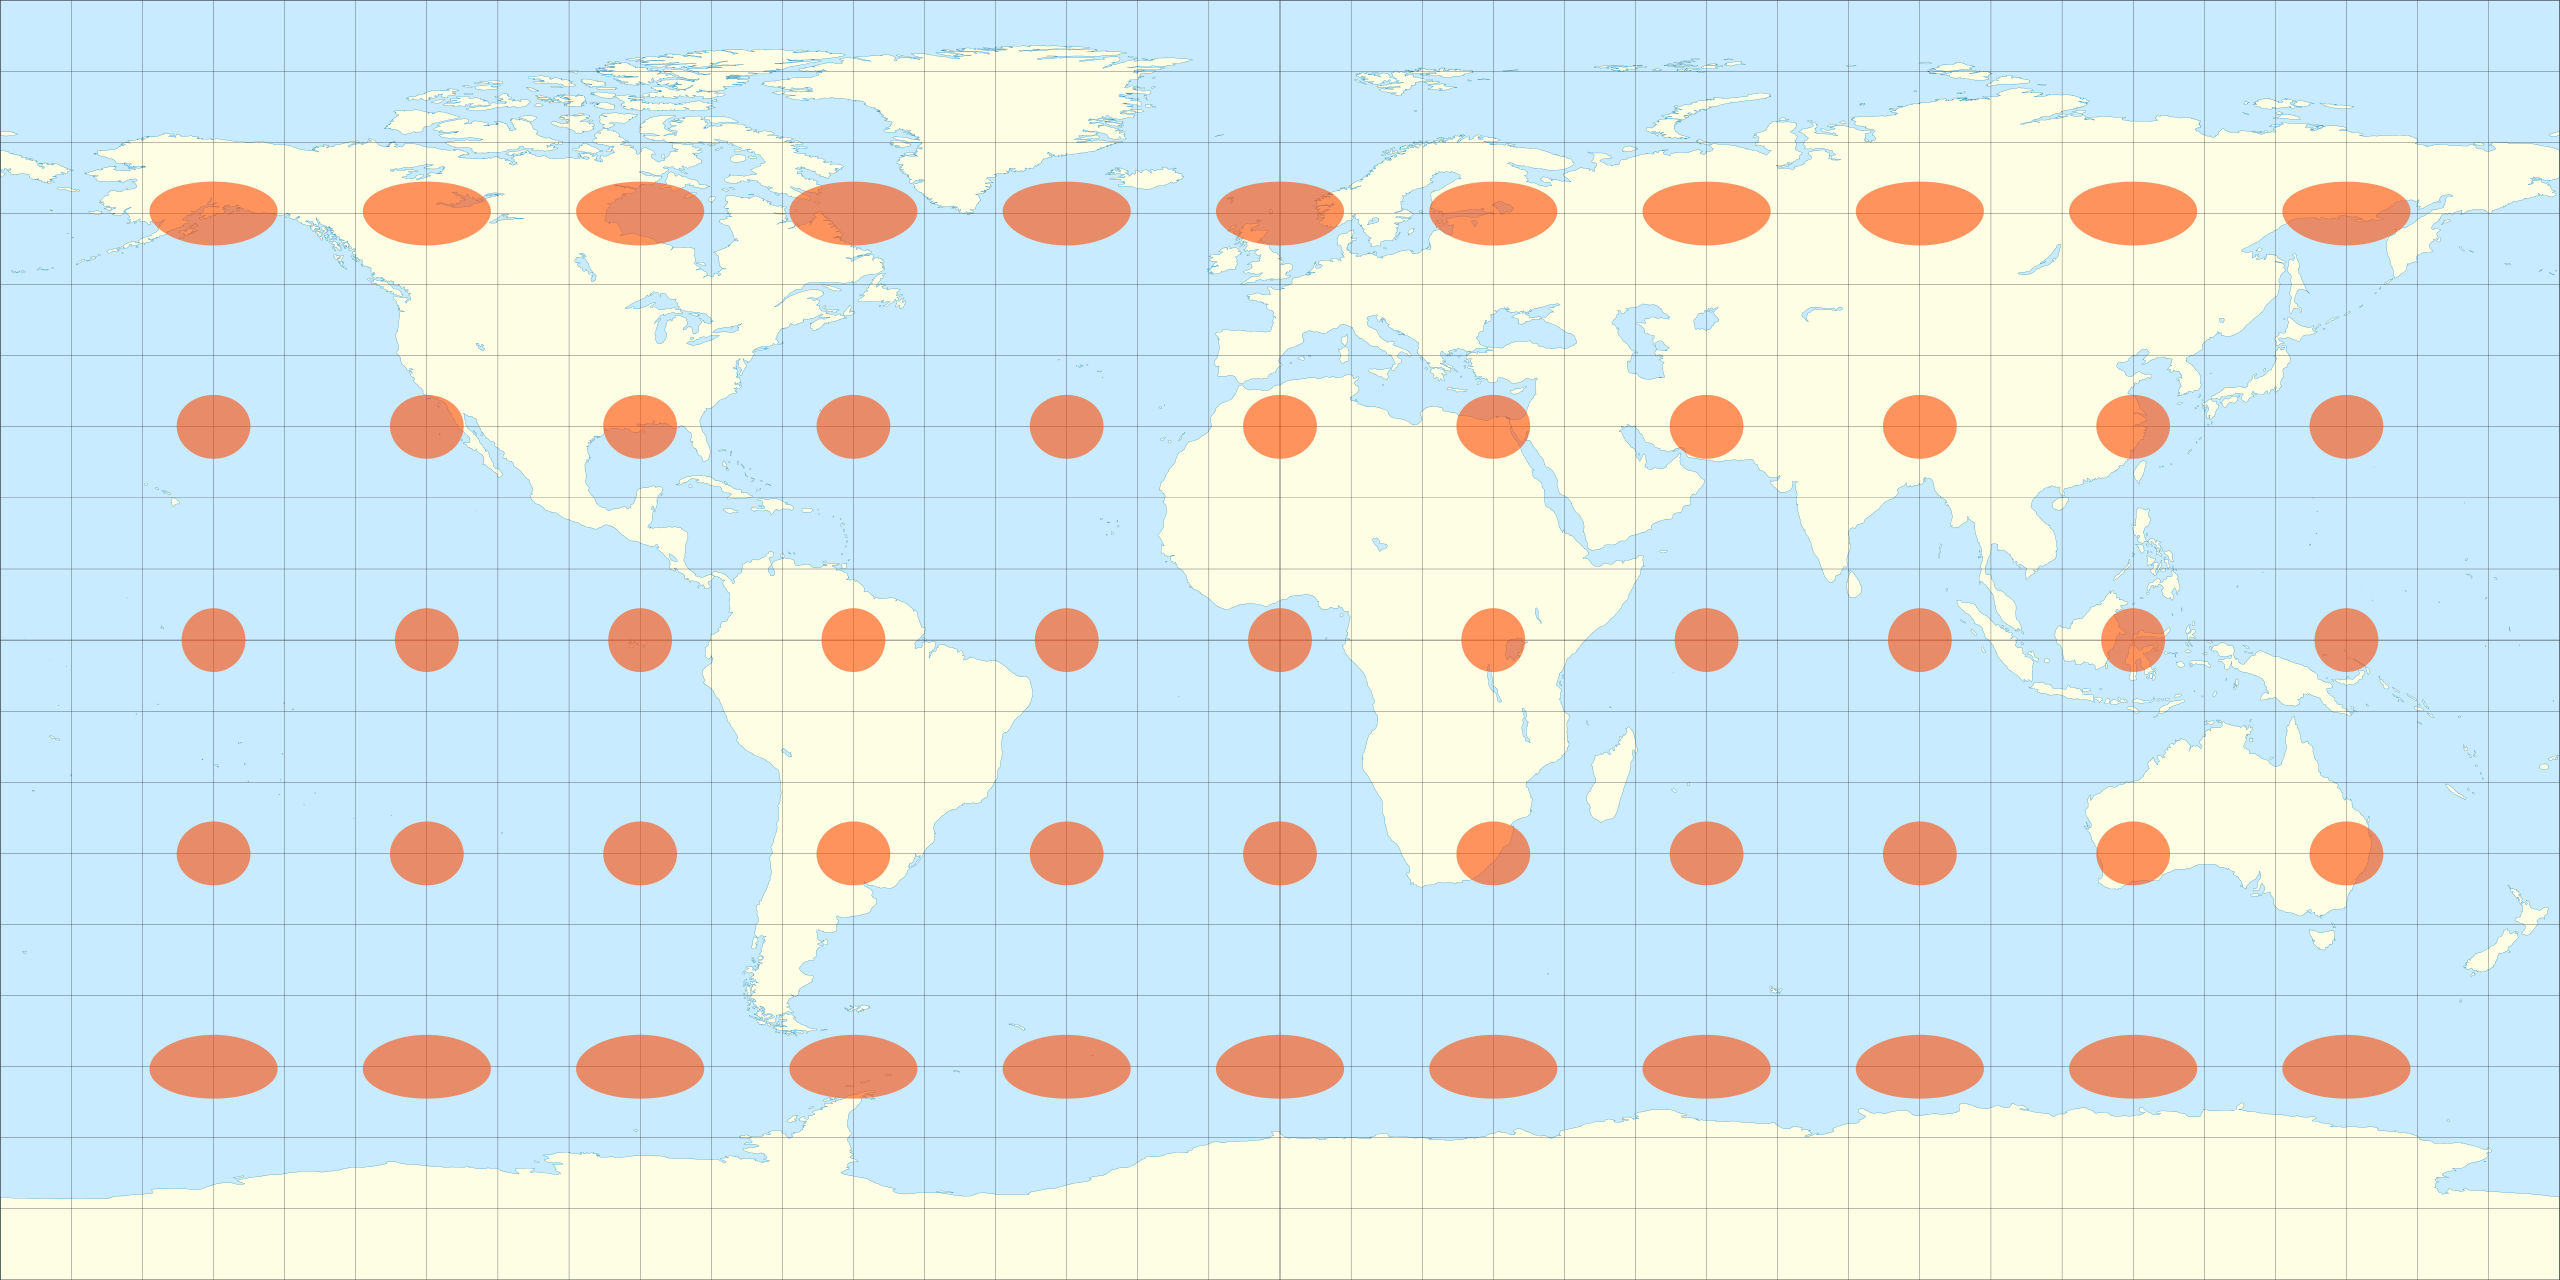
\includegraphics[width=\textwidth]{./Bilder/Tissot_rectangle.png}
\caption{\label{fig_Tissot1}\index{Tissot'sche Indikatrix}%
Tissot'sche Indikatrix zur quadratischen Zylinderprojektion. Die Ellipsen entsprechen den
Darstellungen von Kreisen auf der Kugeloberfl\"ache in der Karte (Quelle \cite{WikiTissot}).}
\end{figure}


Abbildung \ref{fig_Tissot1} zeigt nochmals eine quadratische Zylinderprojektion, bei der die
Abschnitte entlang der L\"angengrade (also in Nord-S\"ud-Richtung)
einen konstanten Abstand haben, d.h., hier werden
die L\"angen- und Breitengrade in einem kartesischen Koordinatensystem dargestellt. 
Wie schon besprochen, f\"uhrt diese Darstellung zu einer Verzerrung in Ost-West-Richtung
in Abh\"angigkeit vom Breitengrad: Je n\"aher der Breitengrad an den Polen ist, umso
gr\"o\ss er ist die Dehnung im Vergleich zum \"Aquator, wo der Ma\ss stab in alle Richtungen
derselbe ist. Ein hypothetischer Kreis auf der Erde (in diesem Fall ein Kreis mit einem 
Radius von rund $r=500$\,km) wird in der Karte durch eine Ellipse wiedergegeben. Diese
Ellipse entartet am \"Aquator zu einem Kreis (dort sind die Ma\ss st\"abe in alle
Richtungen gleich) und wird in Ost-West-Richtung gestreckt, je weiter man sich vom 
\"Aquator entfernt. Auf dem 60.\ Breitengrad ist die gro\ss e Halbachse bereits doppelt so gro\ss\
wie die kleine Halbachse. Beide Halbachsen entsprechen jedoch immer noch auf der
Erdkugel einer Strecke von 500\,km. Man bezeichnet diese Darstellung des ortsabh\"angigen
Kartenma\ss stabs auch als Tissot'sche Indikatrix. Wir nennen die Kartenabbildung von Kreisen auf der
Kugeloberfl\"ache dann Tissot-Ellipsen.\index{Tissot-Ellipse} 
Die Charakterisierung einer Tissot-Ellipse an einem
bestimmten Ort auf der Karte durch die Parameter der Ellipse in Form der Matrix $g_{ij}$
bezeichnet man als metrischen Feldtensor.\index{Feldtensor, metrischer} 
\glqq metrisch\grqq\ bedeutet, dass dieses
Objekt die Ma\ss st\"abe zur Bestimmung von Entfernungen kodiert, \glqq Feld-\grqq\ bedeutet,
dass dieses Objekt an jedem Ort definiert und von Ort zu Ort verschieden sein kann, und 
\glqq Tensor\grqq\ bedeutet, dass es sich um eine Matrix handelt, die die Richtungsabh\"angigkeit
angibt.\footnote{Streng genommen bezieht sich \glqq Tensor\grqq\ darauf, wie sich die Elemente von
$g_{ij}$ unter Koordinatentransformationen ver\"andern, das soll hier aber nicht weiter
vertieft werden.} 

Zur Bestimmung der Parameter $a$ und $b$ k\"onnen wir folgenderma\ss en vorgehen (ein
allgemeines Verfahren, wie man aus einer Parameterdarstellung der Kugeloberfl\"ache diese
Parameter gewinnt, beschreiben wir
in Abschnitt \ref{sec_Parameter}). Die Karte habe eine Breite $B$ (hier ungef\"ahr $B=154$\,mm)
und eine H\"ohe $H=B/2$ (da die Ost-West-Richtung in 360 Grade, die Nord-S\"ud-Richtung
aber nur in 180 Grade unterteilt ist, und beide Richtungen dieselbe Skala haben sollen). 
Der Erdumfang am \"Aquator betr\"agt $U=40\,000$\,km 
(wir gehen hier von einer idealen Kugel mit dieser L\"ange eines Gro\ss kreises aus).
Allgemein: Wenn eine Strecke auf einer Kugel (hier der Umfang) die L\"ange $U$ hat und auf einer Karte 
im Abstand $B$ (hier der Breite der Karte) dargestellt wird, 
dann hat die Karte einen Ma\ss stab von $1:U/B$, hier ungef\"ahr $1:260\,000\,000$.  

Entfernt man sich nun vom \"Aquator in Richtung der Pole \"andert sich
dieser Ma\ss stab in Ost-West-Richtung (d.h.\ f\"ur Punkte auf demselben Breitengrad) 
und der Abstand zwischen zwei L\"angengraden bei einem Breitengrad $\theta$ wird
um den Faktor $\cos \theta$ k\"urzer. Wir erhalten also f\"ur den Ma\ss stab in Ost-West-Richtung am
Breitengrad $\theta$ den Wert $(U/B) \cos \theta$. Damit folgt:
\begin{equation}
           a(\theta,\varphi) = \frac{B}{U\cos \theta} \approx \frac{1}{260\,000\,000 \cos \theta} \hspace{1cm} {\rm und}
           \hspace{1cm}  b(\theta,\varphi) = \frac{B}{U} \approx \frac{1}{260\,000\,000}  \, .  
\end{equation}
Diese Parameter h\"angen nicht von $\varphi$ (dem L\"angengrad) ab sondern nur vom Breitengrad.
Der Ma\ss stab am \"Aquator f\"ur obige Karte (mit der Breite 154\,mm) w\"are somit $1:260\,000\,000$. 
Der metrische Feldtensor w\"are
\begin{equation}
               g = \left( \begin{array}{cc}   \left( \frac{U}{B} \right)^2  \cos^2 \theta & 0 \\ 0 & \left( \frac{U}{B} \right)^2
               \end{array} \right) \, .
\end{equation}
Man erkennt, dass $g_{11}$ bei $\theta=\pm 90^\circ$ (also an den Polen) verschwindet. Hierbei
handelt es sich um eine typische Koordinatensingularit\"at,\index{Koordinatensingularit\"at} 
bei der ein einzelner Punkt
(der Nord- bzw.\ der S\"udpol) auf eine ganze Achse (den oberen bzw.\ unteren Rand der Karte)
abgebildet wird. Der Nord- bzw.\ S\"udpol sind auf der Kugel nat\"urlich vollkommen regul\"are
Punkte. 

\begin{SCfigure}[30][htb]

\includegraphics[trim= 0cm 1.0cm 0.3cm 1.0cm,clip,width=0.6\textwidth]{./Bilder/Zylinderprojektion.jpg}
\thicklines
\begin{picture}(0,0)(250,-50)
\qbezier(33,50)(80,85)(123,57)
\qbezier(33,50)(78,53.5)(123,57)
\end{picture}
\caption{\label{fig_Zylinder2}%
Die k\"urzeste Verbindung auf der Kugeloberfl\"ache zwischen zwei Punkten (z.B.\ Frankfurt und
San Francisco) erscheint auf einer Weltkarte als gekr\"ummte Linie. Allerdings bedarf es weniger
Tissot-Ellipsen, um diese gekr\"ummte Linie zu \"uberdecken als bei der geraden 
Verbindungslinie. (Abbildungsquelle \cite{WikiNetz})}  
\end{SCfigure}
 
\section{Parameterdarstellungen}
\label{sec_Parameter}

Unter einer Parameterdarstellung\index{Parameterdarstellung} 
einer (offenen Teilmenge einer) 2-dimensionalen Mannigfaltigkeit 
(z.B.\ einer Kugeloberfl\"ache), eingebettet in den 3-dimensionalen Raum, versteht man eine Abbildung 
der Form $(u,v) \mapsto \pmb{x}(u,v)$, wobei diese Abbildung lokal bijektiv sein soll.
Wir betrachten zun\"achst nochmals das Beispiel der Kugeloberfl\"ache, die durch die L\"angen- und
Breitengrade parametrisiert wird. 

Eine Kugel l\"asst sich in Kugelkoordinaten\index{Kugelkoordinaten} 
durch die beiden Winkel $\theta$ und $\varphi$ beschreiben:
\begin{equation}
          \pmb{x}(\theta,\varphi) = (R \cos \varphi \cos \theta, R \sin \varphi \cos \theta, R \sin \theta) \, .
\end{equation}
Im Gegensatz zur \"ublichen Wahl von Kugelkoordinaten wurde hier die Parametrisierung
so gew\"ahlt, dass der Winkel $\theta=0$ dem \"Aquator entspricht und $\theta = \pm \frac{\pi}{2}$ dem
Nord- bzw.\ S\"udpol. $\varphi$ kann die Werte $-\pi$ bis $+\pi$ annehmen, wobei $\varphi=0$
den $0$-Meridian bezeichnet. Damit entsprechen $\theta$ und $\varphi$ dem Breiten- bzw.\ L\"angengrad. 
$R$ ist der Radius der Kugel, bei der Erde ist somit $R=40\,000$\,km.  

Eine sehr kleine (infinitesimale) Verschiebung $\Delta \pmb{x}$ auf der Erdkugel, bedeutet f\"ur
die L\"angen- und Breitengrade:
\begin{equation}
       \Delta \pmb{x} = 
       \frac{\partial \pmb{x}}{\partial \theta} \Delta \theta + \frac{\partial \pmb{x}}{\partial \varphi} \Delta \varphi \, ,
\end{equation}
bzw.
\begin{equation}
\label{eq_gthetaphi}
      ( \Delta \pmb{x})^2 = 
       \left( \frac{\partial \pmb{x}}{\partial \theta} \cdot \frac{\partial \pmb{x}}{\partial \theta} \right)
       ( \Delta \theta)^2 + 2 \left( \frac{\partial \pmb{x}}{\partial \varphi} \cdot \frac{\partial \pmb{x}}{\partial \theta} \right)
       \Delta \theta \, \Delta \varphi + \left( \frac{\partial \pmb{x}}{\partial \varphi}\cdot \frac{\partial \pmb{x}}{\partial \varphi}\right)
          (\Delta \varphi )^2 \, .
\end{equation}
Durch Vergleich mit Gl.\ \ref{eq_Ellipse4} erkennen wir die folgenden Beziehungen:
\begin{equation}
       g_{\theta \theta} =   \left( \frac{\partial \pmb{x}}{\partial \theta} \cdot \frac{\partial \pmb{x}}{\partial \theta} \right)
       \hspace{1cm}
       g_{\theta \varphi} = g_{\varphi \theta} =  \left( \frac{\partial \pmb{x}}{\partial \varphi} \cdot \frac{\partial \pmb{x}}{\partial \theta} \right)
       \hspace{1cm}
       g_{\varphi \varphi} = \left( \frac{\partial \pmb{x}}{\partial \varphi}\cdot \frac{\partial \pmb{x}}{\partial \varphi}\right)  \, .
\end{equation}
Berechnen wir die beiden Vektoren
\begin{equation}
       \frac{\partial \pmb{x}}{\partial \theta} = R (- \cos \varphi \sin \theta, - \sin \varphi \sin \theta , \cos \theta)
       \hspace{0.8cm} {\rm und} \hspace{0.8cm} 
       \frac{\partial \pmb{x}}{\partial \varphi} = R (- \sin \varphi \cos \theta, \cos \varphi \cos \theta , 0)
\end{equation}
so folgt:
\begin{equation}
         g_{\theta \theta} = R^2  \hspace{1cm}   g_{\theta \varphi} = g_{\varphi \theta} = 0 
         \hspace{1cm}  g_{\varphi \varphi} = R^2 \cos^2 \theta \, .
\end{equation}
Damit haben wir bez\"uglich der Parametrisierung durch die L\"angen- und Breitengrade den metrischen
Feldtensor gefunden. Allerdings haben wir in Abschnitt \ref{sec_Tissot} die Parametrisierung durch einen
Ma\ss stab auf unserer Karte angeben, d.h.\ die $x$- und $y$-Koordinaten auf der Karte. Wir m\"ussen also noch
die Beziehungen zwischen den L\"angen- und Breitengraden und den $x$- und $y$-Koordinaten der Karte
finden. Die Breite $B$ der Karte entspricht einem Vollkreis von $360^\circ$ oder $2 \pi$, daher folgt
\begin{equation}
\label{eq_Beztheta_z1}
         \varphi = \frac{2\pi}{B} x  \hspace{0.5cm} {\rm und} \hspace{0.5cm} 
         \theta = \frac{2\pi}{B} y \hspace{1cm} {\rm bzw.} \hspace{1cm}
        \Delta \varphi = \frac{2\pi}{B} \Delta x \hspace{0.5cm} {\rm und} \hspace{0.5cm}  
        \Delta \theta = \frac{2\pi}{B} \Delta y  \, .
\end{equation}
Setzen wir diese Beziehungen in Gl.\ \ref{eq_gthetaphi} ein und nutzen aus, dass $U=2\pi R$, folgen die
Beziehungen aus Abschnitt \ref{sec_Tissot}. 

Parametrisieren wir die Kugeloberfl\"ache (oder ganz allgemein eine 2-dimensionale Mannigfaltigkeit
im 3-D-Raum) in der Form $\pmb(u,v)$, dann folgt
\begin{equation}
       \Delta \pmb{x} = 
       \frac{\partial \pmb{x}}{\partial u} \Delta u + \frac{\partial \pmb{x}}{\partial v} \Delta v \, ,
\end{equation}
bzw.
\begin{equation}
\label{eq_g_uv}
      ( \Delta \pmb{x})^2 = 
       \left( \frac{\partial \pmb{x}}{\partial u} \cdot \frac{\partial \pmb{x}}{\partial u} \right)
       ( \Delta u)^2 + 2 \left( \frac{\partial \pmb{x}}{\partial u} \cdot \frac{\partial \pmb{x}}{\partial v} \right)
       \Delta u \, \Delta v + \left( \frac{\partial \pmb{x}}{\partial v}\cdot \frac{\partial \pmb{x}}{\partial v}\right)
          (\Delta v)^2 
\end{equation}
und somit:
\begin{equation}
       g_{u u} =   \left( \frac{\partial \pmb{x}}{\partial u} \cdot \frac{\partial \pmb{x}}{\partial u} \right)
       \hspace{1cm}
       g_{u v} = g_{v u} =  \left( \frac{\partial \pmb{x}}{\partial u} \cdot \frac{\partial \pmb{x}}{\partial v} \right)
       \hspace{1cm}
       g_{v v} = \left( \frac{\partial \pmb{x}}{\partial v}\cdot \frac{\partial \pmb{x}}{\partial v}\right)  \, .
\end{equation}
Die beiden Vektoren $\frac{\partial \pmb{x}}{\partial u}$ und $\frac{\partial \pmb{x}}{\partial v}$ spannen
eine Fl\"ache auf. F\"ur das Quadrat dieser Fl\"ache gilt:
\begin{eqnarray}
               \left( \frac{\partial \pmb{x}}{\partial u} \times \frac{\partial \pmb{x}}{\partial v} \right)^2 &=&
                 \sum_m  \left( \frac{\partial \pmb{x}}{\partial u} \times \frac{\partial \pmb{x}}{\partial v} \right)_m
                  \left( \frac{\partial \pmb{x}}{\partial u} \times \frac{\partial \pmb{x}}{\partial v} \right)_m \\ 
          &=& \sum_{m,i,j,k,l} \epsilon_{mij} \frac{\partial x_i}{\partial u}\frac{\partial x_j}{\partial v}
                        \epsilon_{mkl} \frac{\partial x_k}{\partial u}\frac{\partial x_l}{\partial v}  \\
          &=& \sum_{i,j,k,l}  \Big( \delta_{ik} \delta_{jl} - \delta_{il} \delta_{jk} \Big) 
            \frac{\partial x_i}{\partial u}\frac{\partial x_j}{\partial v} \frac{\partial x_k}{\partial u}\frac{\partial x_l}{\partial v}  \\ 
          &=& \sum_{ij} \left(  \frac{\partial x_i}{\partial u}\frac{\partial x_j}{\partial v} \frac{\partial x_i}{\partial u}\frac{\partial x_j}{\partial v}     
           -       \frac{\partial x_i}{\partial u}\frac{\partial x_j}{\partial v} \frac{\partial x_j}{\partial u}\frac{\partial x_i}{\partial v} \right) \\
         &=&  \left( \sum_{i}  \frac{\partial x_i}{\partial u} \frac{\partial x_i}{\partial u} \right) 
              \left( \sum_{j}  \frac{\partial x_j}{\partial v} \frac{\partial x_j}{\partial v} \right) - 
              \left(  \sum_{i} \frac{\partial x_i}{\partial u} \frac{\partial x_i}{\partial v} \right)
              \left( \sum_j  \frac{\partial x_j}{\partial v} \frac{\partial x_j}{\partial u} \right)  \\
          &=&  g_{uu} g_{vv} - g_{uv}g_{vu} = {\rm det}\, g   \, .     
\end{eqnarray}
Das bedeutet, $\sqrt{{\rm det}\,g}$ gibt den Faktor zwischen einer Fl\"ache auf der Kugeloberfl\"ache und
einer Fl\"ache auf der Karte an: Seien $\Delta \pmb{x}_u$ und $\Delta \pmb{x}_v$ zwei infinitesimale
Verschiebungen auf der Kugeloberfl\"ache, dann gilt:
\begin{equation}
           \Delta \pmb{x}_u = \frac{\partial \pmb{x}}{\partial u} \Delta u  \hspace{1cm} {\rm und} \hspace{1cm}
           \Delta \pmb{x}_v = \frac{\partial \pmb{x}}{\partial v} \Delta v 
\end{equation} 
und somit:
\begin{equation}
\label{eq_LK_df}
   \left| \Delta \pmb{x}_u \times \Delta \pmb{x}_v \right| 
        = \left| \frac{\partial \pmb{x}}{\partial u} \times \frac{\partial \pmb{x}}{\partial v} \right| \, \Delta u \,\Delta v 
        = \sqrt{{\rm det}\,g} \, \Delta u \, \Delta v \, .
\end{equation} 
Wenn $\sqrt{{\rm det}\,g}$ konstant ist (also nicht von dem Ort $u,v$ auf der Karte abh\"angt), bezeichnet
man die Karte als fl\"achentreu.\index{flaechentreu@fl\"achentreu} 
In diesem Fall haben gleiche infinitesimale Fl\"achen $\Delta u \, \Delta v $ auf der Karte auch
gleiche Fl\"achen auf der Kugeloberfl\"ache (und umkehrt). 
Eine Karte hei\ss t winkeltreu oder formtreu bzw.\ konform, wenn\index{winkeltreu}\index{konform} 
\begin{equation}
                       g =  a(u,v) \left( \begin{array}{cc}  1 & 0 \\ 0 & 1 \end{array}   \right) \, . 
\end{equation}
In diesem Fall werden Kreise wieder auf Kreise abgebildet (vgl.\ Gl.\ \ref{eq_Ellipse4}), die allerdings um den 
m\"oglicherweise ortsabh\"angigen Faktor $a(u,v)$ skaliert sind.
      
\section{Zylinder-Projektionen}

Unter einer Zylinderprojektion\index{Zylinderprojektion} 
versteht man eine Abbildung der Kugeloberfl\"ache auf einen Zylinder,
der am \"Aquator (gelegentlich auch an anderen Gro\ss kreisen) 
um die Kugel gelegt wird. Die $x$-Achse entspricht immer den
L\"angengraden und auf der $y$-Achse sind die Breitengrade aufgetragen. Verschiedene Zylinderprojektionen
unterscheiden sich im Wesentlichen in der Skala, die f\"ur die Breitengrade gew\"ahlt wird. 
Die quadratische Zylinderprojektion\index{Zylinderprojektion!quadratische} 
w\"ahlt die $y$-Achse direkt proportional zu den Breitengraden
und zwar mit derselben Skala, wie die L\"angengrade. Daher hat eine solche Karte immer das
Verh\"altnis Breite:H\"ohe$=$2:1.  

\begin{figure}[htb]
\begin{tikzpicture}
\draw[thick] (4,4) circle (2.0 cm);
\draw[thick] (4,7) ellipse  (2.0cm and 0.4cm);
\draw[thick] (4,1) ellipse  (2.0cm and 0.4cm);
\draw[thick] (4,4) ellipse  (2.0cm and 0.4cm);
\draw (4,6) .. controls (5.5,5.2) and (5.5,2.0) .. (4,2);
\draw (5.12,0.65) -- (5.12,6.68);
\draw (0.0,3) node{~};
\draw[thick] (2,1) -- (2,7);
\draw[thick] (6,1) -- (6,7);
\end{tikzpicture}
\hspace{1cm}
%
\begin{tikzpicture}
\draw[thick] (4,3) circle (2.0 cm);
\filldraw[fill=black!100] (4,3) circle (0.06);
\draw (4,3) -- (4.6,4.9);
\draw (4.6,4.9) .. controls (4.9,5.3) and (5.4,5.5) .. (6,5.5);
\draw (4.6,4.9) -- (6,4.9);
\draw (4,3) -- (6,3);
\draw (0.0,0.65) node{~};
\draw[thick] (2,1) -- (2,7);
\draw[thick] (6,1) -- (6,7);
\filldraw[fill=black!100] (6,5.5) circle (0.06);
\filldraw[fill=black!100] (4.6,4.9) circle (0.06);
\filldraw[fill=black!100] (6,4.9) circle (0.06);
\draw (6.15,7.0) node{${\scriptstyle y}$};
\draw (6.3,3) node{${\scriptstyle y=0}$};
\draw (4.53,5.1) node{${\scriptstyle a}$};
\draw (6.15,4.9) node{${\scriptstyle A}$};
\draw (6.2,5.5) node{${\scriptstyle A'}$};
\draw (4.2,3.2) node{${\scriptstyle \theta}$};
\draw (4.4,3.0) arc (0:70:0.4cm);
\end{tikzpicture}
\caption{\label{fig_Zylinderprojektion}%
Zylinderprojektionen. (links) Bei einer Zylinderprojektion wird eine Kugeloberfl\"ache auf einen Zylinder
projiziert, der um einen Gro\ss kreis (meist den \"Aquator) der Kugel gelegt wird, sodass L\"angengrade
in \"aquidistante senkrechte Geraden und Breitengrade in Graden parallel zu der Projektion des
Gro\ss kreises abgebildet werden. (rechts) Die einzige Freiheit besteht in den Abst\"anden der Breitengrade,
d.h.\ in der Beziehung zwischen $\theta$ und  der $y$-Achse. Die Lambert-Projektion ($a\mapsto A$)
projiziert Punkte senkrecht auf die Zylinderfl\"ache, d.h.\ sie behalten ihre H\"ohe. Bei der quadratischen
Zylinderprojektion ($a\mapsto A'$) wird der L\"angenggrad \glqq abgerollt\grqq.} 
\end{figure}


Der Nachteil einer solchen Karte ist, dass die Umrisse von Fl\"achen verzerrt werden -- die Fl\"achen erscheinen
an den Polen in die Breite gezogen -- und dass die Fl\"achen zu den Polen hin gr\"o\ss er erscheinen.
Beide \glqq Fehler\grqq\ lassen sich nicht gleichzeitig beheben. Es gibt aber zwei bekannte Zylinderprojektionen,
bei denen die Fehler einzeln behoben werden: Die Mercator-Projektion ist 
\glqq formtreu\grqq\ oder auch\index{Mercator-Projektion}\index{konform}
konform, d.h., die Form der Fl\"achen bleibt erhalten, allerdings werden die Fl\"achen zu den Polen hin immer
gr\"o\ss er; die Lambert-Projektion ist \glqq fl\"achentreu\grqq, d.h., der Fl\"acheninhalt bleibt erhalten, 
allerdings werden die Formen der Fl\"achen zu den Polen hin verzerrt.

\subsection{Die Lambert-Projektion}
\label{sec_Lambert}

Bei der Lambert-Projektion\index{Lambert-Projektion} 
(genauer sollte man von der zylindrischen Lambert-Projektion sprechen, da Lambert
dieses Darstellungsverfahren auch auf Kegelm\"antel erweitert hat) 
handelt es sich um eine rechteckige Zylinderprojektion, bei der ein Punkt
der Kugeloberfl\"ache senkrecht, ausgehend von der Erdachse, auf die Zylinderfl\"ache projiziert wird. 
Seine H\"ohe auf der Zylinderfl\"ache entspricht also seiner $z$-Koordinate in Kugelkoordinaten. 
Die Gleichungen \ref{eq_Beztheta_z1} werden nun abgewandelt zu:
\begin{equation}
\label{eq_Beztheta_z2}
         \varphi = \frac{2\pi}{B} x  \hspace{0.5cm} {\rm und} \hspace{0.5cm} 
         \sin \theta = \frac{2\pi}{B} y \hspace{1cm} {\rm bzw.} \hspace{1cm}
        \Delta \varphi = \frac{2\pi}{B} \Delta x \hspace{0.5cm} {\rm und} \hspace{0.5cm}  
        \cos \theta \, \Delta \theta = \frac{2\pi}{B} \Delta y  \, .
\end{equation}
Damit folgt nun:
\begin{equation}
         g_{yy} = \frac{U^2}{B^2} \frac{1}{\cos^2 \theta} \hspace{1cm}   g_{xy} = g_{yx} = 0 
         \hspace{1cm}  g_{xx} = \frac{U^2}{B^2} \cos^2 \theta \, .
\end{equation}
Wir erkennen, dass die Wurzel aus der Determinante von $g$, die in zwei Dimensionen die \"Anderung in
der Skala f\"ur infinitesimale Fl\"achen angibt (vgl.\ Gl.\ref{eq_LK_df}), 
konstant ist (Faktor $U^2/B^2$).\footnote{Die Beziehung zwischen der Wurzel der Determinante und
dem Skalenfaktor eines infinitesimalen (Hyper-)Volumens gilt in allen Dimensionen. Daher findet man
bei invarianten Volumenintegralen in $d$ Dimensionen auch immer $\sqrt{{\rm det}\,g}\,{\rm d}^dx$ als
Integrationsma\ss.} 
Das bedeutet, eine
infinitesimale Fl\"ache ${\rm d}f$ auf der Erdkugel ist um den konstanten Faktor $R^2/B^2$ gr\"o\ss er, als
die entsprechende Fl\"ache auf der Karte. Infinitesimal gleiche Fl\"achen auf der Erdkugel werden somit durch
gleiche Fl\"achen auf der Karte wiedergegeben. In diesem Sinne sagt man, die Lambert-Projektion
ist fl\"achenerhaltend oder fl\"achentreu.

\begin{figure}[htb]
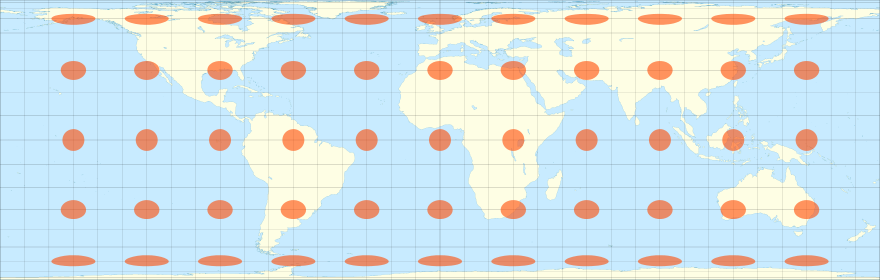
\includegraphics[width=\textwidth]{./Bilder/Lambert.png}
\caption{\label{fig_Lambert}%
Tissot-Darstellung der zylindrischen Lambert-Projektion. (Abbildunsquelle \cite{WikiLambert})}
\end{figure}

Abbildung \ref{fig_Lambert} zeigt eine zylindrische Lambert-Projektion der Erdkugel mit 
Tissot-Ellipsen.\index{Tissot-Ellipse!Lambert-Projektion}
Im Vergleich zu Abb.\ \ref{fig_Tissot1} f\"allt auf, dass die Ellipsen in Poln\"ahe nun flacher sind.
Die Ellipsen nehmen in der H\"ohe um denselben Faktor ab, um den sie in der Breite zunehmen.
Dadurch bleibt der Fl\"acheninhalt der Ellipsen \"uberall derselbe. Allerdings werden die Gebiete in
Poln\"ahe auch st\"arker in der H\"ohe zusammengepresst und im Vergleich zu einer formgetreuen
Darstellung verzerrt. Nun werden beide diagonalen Komponenten im metrischen Tensor an den Polen
singul\"ar.

\subsection{Die Mercator-Projektion}  
\label{sec_Mercator}

Obwohl man die Mercator-Projektion\index{Mercator-Projektion} 
als rechteckige Zylinderprojektion bezeichnet, handelt es sich
im strengen Sinne nicht um eine Projektion, da die Abbildung eines Punkts auf der Kugeloberfl\"ache
auf einen Punkt auf der Zylinderoberfl\"ache keine geometrische Konstruktion ist. Trotzdem besteht auch hier
die einzige Ver\"anderung zur quadratischen Zylinderprojektion in der Beziehung zwischen der
$y$-Achse und dem Breitengrad. 

Die Mercator-Projektion ist lokal winkel- und formtreu. Diese beiden Begriffe sind insofern
\"aquivalent, als aus lokaler Winkeltreue die lokale Formtreue folgt und umgekehrt: Wenn zwei
Dreiecke dieselben Winkel haben, haben sie auch die gleiche Form bzw.\ sind sich \"ahnlich, d.h., die 
Verh\"altnisse von je zwei Seitenl\"angen sind gleich. Die Mercator-Projektion ist nach Gerhard Mercator
(1512-1597)\index{Mercator, Gerhard} 
benannt, der diese Projektionen um 1570 zum ersten Mal f\"ur Weltkarten verwendete.
Die lokale Winkeltreue der Karte war fr\"uher in der Seefahrt von Vorteil, da ein bestimmter Kurs nach
dem Kompass (der den Winkel zu einem L\"angengrad angibt) einer geraden Linie entspricht. 
\"Uber gro\ss e Abst\"ande ist das aber nicht die k\"urzeste Verbindung zwischen zwei Punkten.
Gro\ss kreise (die die k\"urzeste Verbindung darstellen) werden auf Mercator-Karten nicht als
Geraden dargestellt. 

\begin{SCfigure}[30][htb]
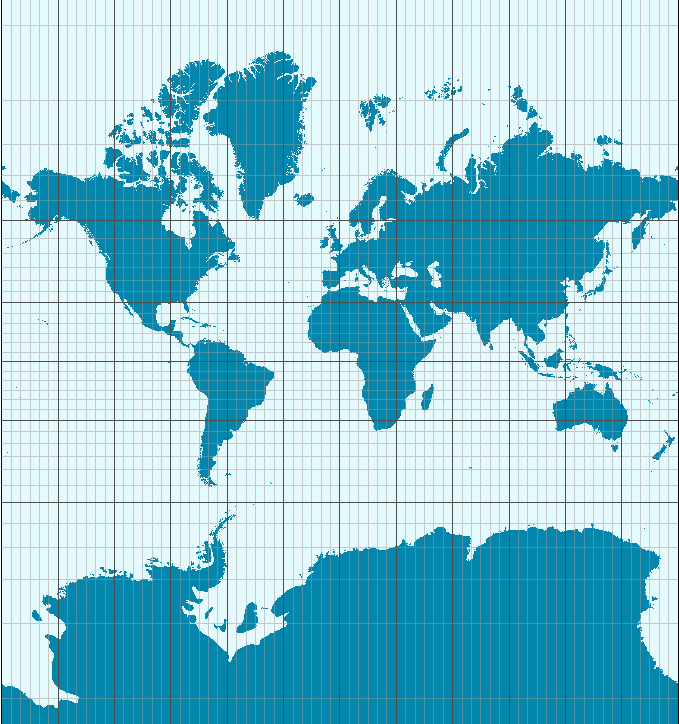
\includegraphics[trim= 0cm 1.0cm 0.3cm 1.0cm,clip,width=0.45\textwidth]{./Bilder/Mercator-proj.png}
\caption{\label{fig_Mercator}%
Eine Weltkarte in Mercator-Darstellung. In \"Aquatorn\"ahe gleicht diese Karte der
quadratischen Zylinderprojektion (Abb.\ \ref{fig_Zylinder}). Allerdings wird der Ma\ss stab in
Poln\"ahe nicht nur in die Breite sondern auch in die H\"ohe gestreckt. Dadurch erscheinen
die Umrisse von kleineren L\"andern zwar \"ahnlich wie auf einer lokalen Projektion, also
entsprechend ihrer lokalen Form, doch wirken
die L\"ander im Vergleich zu Gebieten am \"Aquator \"ubertrieben gro\ss. Afrika ist in Wirklichkeit
\"uber f\"unfzehnmal gr\"o\ss er als Gr\"onland, Australien ist viermal gr\"o\ss er. Afrika ist 
mehr als doppelt so gro\ss\ wie das Landgebiet der Antarktis. (Quelle \cite{WikiMercator})}  
\end{SCfigure}

Damit eine Karte formtreu ist, m\"ussen lokal die Abst\"ande in $x$-Richtung und in $y$-Richtung
um denselben Ma\ss stab ver\"andert werden, d.h., die beiden diagonalen Komponenten in der Metrik
sind gleich (aber ortsabh\"angig). Da wir bei der Parametrisierung nur die Beziehung zwischen dem
Breitengrad $\theta$ und der H\"ohe $y$ ver\"andern k\"onnen, ist eine Beziehung gesucht, sodass
\begin{equation}
     g = \frac{U^2}{B^2} \cos^2 \theta \left( \begin{array}{cc} 1 & 0 \\ 0 & 1 \end{array} \right)  
     \hspace{1cm} {\rm bzw.} \hspace{1cm}    \Delta \theta = \frac{2\pi}{B} \cos \theta\,  \Delta y \, .
\end{equation}
Zur Bestimmung von $y(\theta)$, der $y$-Koordinate auf der Karte als Funktion des Breitengrads,
haben wir somit das Integral
\begin{equation}
                     y(\theta) = \frac{B}{2\pi} \int_{0}^\theta \frac{1}{\cos \theta'} {\rm d}\theta'  
\end{equation}
zu l\"osen. Die L\"osung lautet:
\begin{equation}
                     y(\theta) = \frac{B}{2\pi}  \ln \sqrt{ \frac{1 - \sin \theta}{1+\sin \theta} }\, .
\end{equation}
Zur L\"osung des Integrals: Man erweitere den Integranden im Z\"ahler und Nenner um $\cos \theta'$, ersetze
im Z\"ahler $\cos \theta' \, {\rm d}\theta' = {\rm d} \sin \theta'$ und im Nenner $\cos^2\theta' = 1 - \sin^2 \theta'$.
Mit einer Partialbruchzerlegung, 
$\frac{1}{(1-\sin^2 \theta')} = \frac{1}{2} (\frac{1}{1-\sin \theta'} + \frac{1}{1+\sin \theta'})$
kann man das Integral leicht l\"osen. 

F\"ur kleine Werte von $\theta$, also in \"Aquatorn\"ahe, verh\"alt sich obige Beziehung wie in Gl.\ \ref{eq_Beztheta_z1},
aber f\"ur $\theta \rightarrow \frac{\pi}{2}$ divergiert dieser Ausdruck, d.h., der Nord- bzw.\ S\"udpol sind auf einer
Mercator-Karte im Unendlichen. Daher h\"oren die meisten Mercator-Karten auch etwas oberhalb des
$80$.\ Breitengrads auf (Abb.\ \ref{fig_Mercator} endet ungef\"ahr beim 83.\ Breitengrad) 

\section{Das UNO-Emblem}

\begin{SCfigure}[30][htb]

\includegraphics[trim= 0cm 1.0cm 0cm 1.0cm,clip,width=0.35\textwidth]{./Bilder/un_PNG20.png}
\caption{\label{fig_UN}%
Das Logo der Vereinten Nationen. In diesem Fall handelt es sich um eine sogenannte
Azimutalprojektion. Es wird eine Ebene an einen Punkt der Kugel gelegt (in diesem Fall
den Nordpol) und die Erdkugel wird in Polarkoordinaten um diesen Punkt herum dargestellt. 
Im vorliegenden Fall sind die Breitengrade von $90^\circ$-Nord bis rund $50^\circ$-S\"ud wiedergegeben.
Die Einteilung der Breitengrade ist in $30^\circ$-Schritten und die Breitengrade sind
\"aquidistant dargestellt. (Quelle \cite{UN})}  
\end{SCfigure}

Die Flagge der Vereinten Nationen (Abb.\ \ref{fig_UN})\index{Vereinte Nationen, Logo}
verwendet eine Darstellung der Erdkontinente in Polarkoordinaten - eine sogenannte 
Azimutalprojektion.\index{Azimutalprojektion}
In diesem Fall wird eine Ebene tangential an einen Punkt der Kugel gelegt (sehr h\"aufig, wie auch bei dem
UN-Logo, an den Nordpol) und die Kugeloberfl\"ache wird in Polarkoordinaten auf diese Fl\"ache
projiziert. Diese Darstellung (Nordpol als zentraler Punkt) wird auch hier gew\"ahlt.
Der Polarwinkel $\varphi$ entspricht dem L\"angengrad (allerdings wird im UN-Logo der
L\"angengrad $0$ nach unten projiziert). Die Breitengrade sind dann konzentrische Kreise um den
Nordpol. Der Abstand zwischen Breitengraden ist der einzige Freiheitsgrad, der hier gew\"ahlt
werden kann. Im UN-Logo sind die Breitengrade \"aquidistant angeordnet. Es gibt auch
fl\"achentreue Darstellungen, bei denen der Abstand zwischen Breitengraden von Nord nach
S\"ud abnimmt. Theoretisch gibt es auch eine konforme Abbildung, bei der die Fl\"achenform
erhalten bleibt, diese w\"urde sich aber nach Unendlich erstrecken und die L\"ander s\"udlich des
\"Aquators w\"aren \"ubertrieben gro\ss\ dargestellt. Azimutale Projektionen sind nur an einem
Punkt der Kugeloberfl\"ache singul\"ar, in diesem Fall am S\"udpol. 

Polarkoordinaten sind 2-dimensionale Koordinaten in der Ebene, gegeben durch\index{Polarkoordinaten}
\begin{equation}
          \pmb{x}(r,\varphi) = (r\cos \varphi, r \sin \varphi)  \, .
\end{equation}
(Wir w\"ahlen hier die \"ubliche Konvention, bei der $\varphi=0$ dem Punkt $(x,y)=(1,0)$ entspricht.
Die UN-Darstellung erh\"alt man aus der Koordinatenwahl $(x,y)=(r\sin \varphi, -r\cos \varphi)$.) Der
Winkel $\varphi$ entspricht direkt dem L\"angengrad. Der Breitengrad $\theta$ auf der Kugeloberfl\"ache
entspricht hier dem Radius, d.h.\ je nach Wahl der Darstellung ist $r=r(\theta)$ eine andere
Funktion. 

F\"ur Polarkoordinaten gilt die Beziehung:
\begin{equation}
           (\Delta s)^2 = (\Delta r)^2 + r^2 (\Delta \varphi)^2  \, .
\end{equation} 
Damit ist
\begin{equation}
     g =  \left( \begin{array}{cc} 1 & 0 \\ 0 & r^2 \end{array} \right) \hspace{1cm} {\rm bzw.} \hspace{0.7cm}
           (\Delta s)^2 = g_{rr} (\Delta r)^2 + (g_{r\varphi}+g_{\varphi r} ) \Delta r \Delta \varphi + g_{\varphi \varphi} (\Delta \varphi)^2  \, .     
\end{equation}
Wir erhalten diese Metrik wieder aus der Forderung
\begin{equation}
       g_{u u} = \frac{\partial \pmb{x}(u,v)}{\partial u} \cdot \frac{\partial \pmb{x}(u,v)}{\partial u} \hspace{0.7cm}
       g_{u v} = g_{v u} = \frac{\partial \pmb{x}(u,v)}{\partial u} \cdot \frac{\partial \pmb{x}(u,v)}{\partial v} \hspace{0.7cm}
       g_{v v} = \frac{\partial \pmb{x}(u,v)}{\partial v} \cdot \frac{\partial \pmb{x}(u,v)}{\partial v}   
\end{equation}
mit den Tangentialvektoren:
\begin{equation}
       \frac{\partial \pmb{x}(r,\varphi)}{\partial r} = (\cos \varphi, \sin \varphi) \hspace{1cm}
       \frac{\partial \pmb{x}(r,\varphi)}{\partial \varphi} = (- r\sin \varphi, r\cos \varphi)  \, .
\end{equation}

Wir m\"ussen nun noch die Beziehung zwischen $r$ auf unserer Karte (in Polarkoordinaten) und den
Breitengraden $\theta$ auf der Kugeloberfl\"ache herstellen. Die Winkel $\varphi$ sind in beiden F\"allen
gleich. Wenn wir den Durchmesser der Karte mit $D$ bezeichnen, entspricht $D$ einem Vollkreis, sodass
$r= D/(2\pi) \theta$. Umgekehrt entspricht auf der Erdkugel der Differenz von Breitengraden $\Delta \theta$ eine
Strecke von $\Delta l = R \Delta \theta = (U/2\pi) \Delta \theta$. Insgesamt erhalten wir somit:
\begin{equation}
                  \Delta r = \frac{D}{2\pi} \Delta \theta = \frac{D}{2\pi} \frac{2\pi}{U} \Delta l = \frac{D}{U} \Delta l \, , 
\end{equation}  
und misst man die L\"ange $l$ vom Nordpol aus zu einem Punkt auf der Erdkugel, gilt auch
$r=\frac{D}{U} l$. 

\section{Kuriosit\"aten}

\subsection{Tissot-Figuren in h\"oheren Dimensionen}

In drei Dimensionen wird eine\index{Tissot-Figur} 
Tissot-Figur zu einem Ellipsoid. Ein Ellipsoid ist gekennzeichnet durch
die drei Hauptachsen sowie die Lage im Raum (nochmals drei Winkel, d.h.\ sechs Parameter). Dies
l\"asst sich durch eine symmetrische $3\times 3$-Matrix $g_{ij}$ charakterisieren, sodass die Ellipsoid-Gleichung die Form
\begin{equation}
               (\Delta s)^2 = \sum_{i,j=1}^3 g_{ij} \Delta x_i  \Delta x_j    
\end{equation}
annimmt. Diese Gleichung bleibt unver\"andert auch in h\"oheren Dimensionen, lediglich die Indizes 
durchlaufen eine gr\"o\ss ere Indexmenge. Da $g$ symmetrisch (und damit selbst-adjungiert) ist, kann
man es durch eine Rotation diagonalisieren. Die Eigenwerte sind $\lambda_i=1/a_i^2$, wobei $a_i$ die
Hauptachsen des verallgemeinerten Ellipsoids sind, und die Rotation charakterisiert die Lage dieser
Hauptachsen im Raum.

\subsection{Tissot-Hyperbeln in Minkowski-R\"aumen}

In $(1+1)$-Raumzeit-Dimensionen handelt es sich bei den Tissot-Figuren um Hyperbeln und
die Vorgabe der Lichtkegelstruktur.\index{Tissot-Hyperbel} 
Die Kreisgleichung wird ersetzt durch
\begin{equation}
                          (\Delta t)^2 - (\Delta x)^2 = {\rm const.}   \, .
\end{equation} 
Ist die Konstante positiv, spricht man von\index{zeitartig}\index{raumartig} 
zeitartigen Ereignissen (die sich in ihrer
Lage um $\Delta t$ und $\Delta x$ unterscheiden). Ist sie negativ nennt man die Ereignisse
raumartig, und ist sie null, sind die Ereignisse lichtartig.\index{lichtartig} 
In diesen Koordinaten werden die
Lichtkegel durch Diagonalen dargestellt und die Skala ist in zeitartige und raumartige Richtungen
dieselbe. In einer allgemeinen Karte k\"onnen die Lichtkegel lokal gedreht sein und die Skalen
auch unterschiedlich. In h\"oher dimensionalen R\"aumen werden die Lichtkegel zu verallgemeinerten
Kegelmantelfl\"achen, die zeitartigen \glqq Hyperbeln konstanter Eigenzeiten\grqq\ werden zu
 \glqq Hyperbelschalen konstanter Eigenzeiten\grqq, die raumartigen Hyperbeln konstanter Abst\"ande
 werden zu Rotationsk\"orpern, die durch Drehung um die Zeitachse entstehen.

\subsection{Die Lambert-Karte und ein Theorem von Archimedes}

Eines der drei bekannten mathematischen Probleme der Antike war die geometrische Konstruktion --
nur mit Zirkel und Lineal -- eines Quadrats mit derselben Fl\"ache wie ein vorgegebener Kreis
bzw.\ letztendlich die Konstruktion der Zahl $\pi$ aus einer Einheitsl\"ange. Der Beweis, dass
dies nicht m\"oglich ist, erfolgte erst 1882 durch\index{Lindemann, Ferdinand} 
Ferdinand Lindemann. Genauer hat Lindemann
bewiesen, dass $\pi$ trans\-zendent ist (also keine L\"osung einer algebraischen Gleichung mit rationalen
Koeffzienten ist); dass sich transzendente Zahlen nicht geometrisch mit Zirkel und Lineal
konstruieren lassen, war schon vorher bekannt. 

Archimedes\index{Archimedes} 
konnte jedoch sehr viele Theoreme beweisen, bei denen krummlinige Fl\"achen
mit Quadraten oder Rechtecken in Beziehung gebracht wurden. Eines dieser Theoreme
besagt, dass die Oberfl\"ache einer Kugel genauso gro\ss\ ist wie die Mantelfl\"ache eines
Zylinders, der am \"Aquator um die Kugel gewickelt ist und dieselbe H\"ohe wie die Kugel hat. 
Heute w\"urden wir das folgenderma\ss en beweisen: Die Oberfl\"ache einer Kugel vom Radius $R$
ist $4\pi R^2$, ein um die Kugel gewickelter Zylinder hat die Grundseite $U=2\pi R$ (der Umfang
der Kugel) und die H\"ohe $2R$ und damit die Fl\"ache $2R\cdot 2\pi R = 4\pi R^2$. Manchmal
hei\ss t es auch, dass die Gesamtfl\"ache des umschriebenen Zylinders gleich $3/2$ mal
die Kugeloberfl\"ache ist: Die beiden Deckel haben zusammen eine Fl\"ache von $2 \cdot \pi R^2$; womit
man auch dieses Ergebnis leicht erh\"alt.   

\begin{SCfigure}[30][htb]
\begin{tikzpicture}
\draw (0.2,0.3) node{~};
\draw[thick] (2,2) circle (1.4 cm);
\draw[thick] (0.6,0.6) -- (0.6,3.4);
\draw[thick] (3.4,0.6) -- (3.4,3.4);
\draw[thick] (2,0.6) ellipse  (1.4cm and 0.2cm);
\draw[thick] (2,3.4) ellipse  (1.4cm and 0.2cm);
%\draw[thick] (6,1) -- (6,7);
\end{tikzpicture}
\caption{\label{fig_Archimedes}%
Die Archimedes-Figur. Angeblich wollte Archimedes, dass diese Figur auf seinem Grabstein abgebildet
wird. Dargestellt ist eine Kugel, die einem Zylinder gleicher H\"ohe eingeschrieben ist. 
Archimedes konnte beweisen, dass die Oberfl\"ache der Kugel gleich der Mantelfl\"ache des
Zylinders ist.} 
\end{SCfigure}

Angeblich wollte Archimedes auf seinem Grabstein die Figur aus Abb.\ \ref{fig_Archimedes} 
abgebildet haben, weil er die Beziehung zwischen der Kugeloberfl\"ache und der Mantelfl\"ache
des Zylinders als seine gr\"o\ss te Entdeckung ansah. Eigentlich hat Archimedes sogar mehr
bewiesen, als dass die Gesamtfl\"achen gleich sind; er hat bewiesen, dass kleine Ausschnitte
der Kugeloberfl\"ache, die man im Sinne der Lambert-Projektion von der Zylinderachse aus
auf die Zylinderfl\"ache projiziert, auf Fl\"achen derselben Gr\"o\ss e abgebildet werden. Damit
hat er die Fl\"achentreue der Lambert-Projektion bewiesen. 

Archimedes hat bei vielen seiner mathematischen Beweise sehr physikalisch gedacht und
oft infinitesimale Fl\"achen in Gedanken auf eine Balkenwaage gelegt und die Hebelgesetze
genutzt, um Beziehungen zwischen diesen Fl\"achen abzuleiten.  
Sehr oft kann man solche Operationen mit dem Strahlensatz und dem
Satz von den gleichen Verh\"altnissen von sich entsprechenden Seitenl\"angen in \"ahnlichen 
Dreiecken in Verbindung bringen. Der folgende Beweis nutzt nur diese beiden S\"atze.

\begin{figure}[htb]
\begin{tikzpicture}
\draw (0.0,0.0) node{~};
\draw (3,2.5) circle (2.5 cm);
\draw (0.5,0) -- (0.5,5);
\draw (0.5,2.5) -- (5.5,2.5);
\draw (3.0,0) -- (3.0,5);
\draw (0.5,3.8) -- (3.0,3.8);
\draw (0.5,4.2) -- (3.0,4.2);
\draw (3.0,2.5) -- (0.88,3.8);
\draw (0.88,2.5) -- (0.88,4.2);
\draw[thick] (0.52,3.8) -- (0.52,4.2);
\draw[thick] (2.98,3.8) -- (2.98,4.2);
\draw[thick] (0.88,3.8) -- (1.18,4.2);
\draw (0.4,4.0) node{${\scriptstyle h}$};
%\draw (3.13,4.0) node{${\scriptstyle h}$};
\draw (1.2,4.0) node{${\scriptstyle h'}$};
\draw (1.75,3.05) node{${\scriptstyle R}$};
\draw (2.0,3.7) node{${\scriptstyle R'}$};
\end{tikzpicture}
\hspace{1cm}
%
\begin{tikzpicture}
\draw (0.0,0.0) node{~};
\draw (5.5,5.0) arc (90:180:5cm);
\draw (0.5,0.0) -- (5.5,0.0);
\draw (0.5,0.0) -- (0.5,5.0);
\draw (5.5,0) -- (5.5,5);
\draw (0.5,2.6) -- (5.5,2.6);
\draw (0.5,3.4) -- (5.5,3.4);
\draw (5.5,0.0) -- (1.22,2.6);
\draw (1.22,0.0) -- (1.22,3.4);
\draw[thick] (0.52,2.6) -- (0.52,3.4);
\draw[thick] (5.48,2.6) -- (5.48,3.4);
\draw[thick] (1.22,2.6) -- (1.84,3.4);
\draw (0.4,3.0) node{${\scriptstyle h}$};
%\draw (5.63,3.0) node{${\scriptstyle h}$};
\draw (1.78,3.0) node{${\scriptstyle h'}$};
\draw (3.0,1.3) node{${\scriptstyle R}$};
\draw (3.5,2.45) node{${\scriptstyle R'}$};

\draw (5.55,0.0) node{${\scriptstyle A}$};
\draw (1.1,0.12) node{${\scriptstyle B}$};
\draw (1.1,2.72) node{${\scriptstyle C}$};
\draw (1.8,3.56) node{${\scriptstyle A'}$};
\draw (1.2,3.56) node{${\scriptstyle B'}$};

\end{tikzpicture}
\caption{\label{fig_Archimedes2}%
Zum geometrischen Beweis der Fl\"achentreue der Lambert-Projektion.
Die rechte Seite zeigt den Ausschnitt links-oben vergr\"o\ss ert. Da die Strecke
$A'C$ senkrecht auf $AC$ steht, sind die Dreiecke $ABC$ und $A'B'C$ \"ahnlich.
Daraus folgt $R'/R = h/h'$. 
} 
\end{figure}

In Abbildung \ref{fig_Archimedes2} (rechts) sind die beiden Dreiecke
$ABC$ und $A'B'C$ \"ahnlich. Das bedeutet: $h/h' = R'/R$. Stellen wir uns nun vor,
die infinitesimale Strecke $h$ auf dem Zylinder wird einmal um die zentrale
Zylinderachse rotiert, dann ist die \"uberstrichene Fl\"ache gleich $2\pi R h$. 
Die entsprechende Fl\"ache f\"ur das Streckenst\"uck $h'$ ist $2\pi h' R'$. Doch wegen
$h/h'=R'/R$ folgt, dass diese beiden Fl\"achen gleich sind. Diese Aussage gilt
nicht nur f\"ur den vollen Rotationsk\"orper, sondern auch f\"ur die \"uberstrichenen
Fl\"achen bei beliebig kleinen Rotationswinkel.\index{Landkarten|)}  


\begin{thebibliography}{99}
\bibitem{WikiNetz} Wikipedia \glqq Kartennetzentwurf\grqq:\\
    \url{https://commons.wikimedia.org/wiki/File:Zylinderprojektion_quadratische_plattkarte_kl.jpg}
\bibitem{WikiTissot} Wikipedia \glqq Tissot'sche Indikatrix\grqq:\\ 
       \url{https://de.wikipedia.org/wiki/Tissotsche_Indikatrix}
\bibitem{WikiLambert} Wikipedia \glqq Projection \'{e}quivalente cylindrique de Lambert\grqq;\\ 
    \url{https://upload.wikimedia.org/wikipedia/commons/thumb/c/cb/Tissot_indicatrix_world_map_Lambert_cyl_equal-area_proj.svg/880px-Tissot_indicatrix_world_map_Lambert_cyl_equal-area_proj.svg.png}
\bibitem{WikiMercator} Wikipedia \glqq Gerhard Mercator\grqq;\\ 
        \url{https://upload.wikimedia.org/wikipedia/commons/f/fa/Mercator-proj.png}
\bibitem{UN} UN-Logo:\\
            \url{https://pngimg.com/uploads/un/un_PNG20.png}

\end{thebibliography}

%\end{document}


%
%\documentclass[german,10pt]{book}     
\usepackage{makeidx}
\usepackage{babel}            % Sprachunterstuetzung
\usepackage{amsmath}          % AMS "Grundpaket"
\usepackage{amssymb,amsfonts,amsthm,amscd} 
\usepackage{mathrsfs}
\usepackage{rotating}
\usepackage{sidecap}
\usepackage{graphicx}
\usepackage{color}
\usepackage{fancybox}
\usepackage{tikz}
\usetikzlibrary{arrows,snakes,backgrounds}
\usepackage{hyperref}
\hypersetup{colorlinks=true,
                    linkcolor=blue,
                    filecolor=magenta,
                    urlcolor=cyan,
                    pdftitle={Overleaf Example},
                    pdfpagemode=FullScreen,}
%\newcommand{\hyperref}[1]{\ref{#1}}
%
\definecolor{Gray}{gray}{0.80}
\DeclareMathSymbol{,}{\mathord}{letters}{"3B}
%
\newcounter{num}
\renewcommand{\thenum}{\arabic{num}}
\newenvironment{anmerkungen}
   {\begin{list}{(\thenum)}{%
   \usecounter{num}%
   \leftmargin0pt
   \itemindent5pt
   \topsep0pt
   \labelwidth0pt}%
   }{\end{list}}
%
\renewcommand{\arraystretch}{1.15}                % in Formeln und Tabellen   
\renewcommand{\baselinestretch}{1.15}                 % 1.15 facher
                                                      % Zeilenabst.
\newcommand{\Anmerkung}[1]{{\begin{footnotesize}#1 \end{footnotesize}}\\[0.2cm]}
\newcommand{\comment}[1]{}
\setlength{\parindent}{0em}           % Nicht einruecken am Anfang der Zeile 

\setlength{\textwidth}{15.4cm}
\setlength{\textheight}{23.0cm}
\setlength{\oddsidemargin}{1.0mm} 
\setlength{\evensidemargin}{-6.5mm}
\setlength{\topmargin}{-10mm} 
\setlength{\headheight}{0mm}
\newcommand{\identity}{{\bf 1}}
%
\newcommand{\vs}{\vspace{0.3cm}}
\newcommand{\noi}{\noindent}
\newcommand{\leer}{}

\newcommand{\engl}[1]{[\textit{#1}]}
\parindent 1.2cm
\sloppy

             \begin{document}  \setcounter{chapter}{0}


\setcounter{page}{1}
\setcounter{section}{0}
\setcounter{figure}{0}
\setcounter{equation}{0}
\setcounter{table}{0}
\setcounter{footnote}{0}

\section*{Grundlagen der SRT}
\noindent
{\bf Thomas Filk; Universit\"at Freiburg}
% Kap x
\vspace{1cm}

\label{chap_Grundlagen}

\noindent
Gegen Ende des 19.\ Jahrhunderts mehrten sich die
Anzeichen, dass irgendetwas im Weltbild der Physik
nicht stimmen konnte. Die Newton'sche Mechanik war
sehr erfolgreich bei der Beschreibung der Bewegungen
von materiellen K\"orpern, insbesondere den Bewegungen der Planeten. Andererseits war die
Theorie Maxwell's ebenso erfolgreich bei der 
Beschreibung der Ph\"anomene im Zusammenhang mit
elektrischen und magnetischen Feldern. Doch die beiden Theorien passten nicht zusammen:
Die Newton'sche Theorie ist fundamental Galilei-invariant, d.h.\ mit jeder Bahnkurve $x(t)$, 
die eine L\"osung der Bewegungsgleichungen ist, ist auch eine Galilei-transformierte Bahnkurve, 
$\hat{x}(t)= x(t)+vt+a$, eine L\"osung der Bewegungsgleichungen. Hierbei ist $v$ eine konstante
Geschwindigkeit und $a$ eine konstante Verschiebung. $x(t)$ kann sich auch auf mehrere Komponenten
und mehrere Objekte beziehen. 
  
Die Maxwell'sche Theorie enth\"alt jedoch als Parameter eine Geschwindigkeit (die 
Lichtgeschwindigkeit im Vakuum) und scheint somit ein
spezielles Ruhesystem auszuzeichnen. Dieses Ruhesystem dachte man sich gleichzeitig als
Ruhesystem eines \"Athers, dessen oszillatorische Anregungen den elektromagnetischen Wellen
entsprechen sollten, \"ahnlich wie die Schwingungen von Luft den Schallwellen entsprechen. Das
Experiment von Michelson und Morley (siehe Abschnitt \ref{sec_Michelson}) war dazu gedacht, 
dieses Ruhesystem experimentell zu bestimmen. 

Oftmals wird der Ausgang des Michelson-Morley-Experiments
als Beweis daf\"ur gewertet, dass es den \"Ather bzw.\
das ausgezeichnete Ruhesystem nicht gibt. Das ist
streng genommen nicht richtig: Die dynamischen
Erkl\"arungen von Lorentz und Fitzgerald (wonach
sich Gegenst\"ande bei einer Bewegung relativ zum
\"Ather verk\"urzen und alle Zeitabl\"aufe entsprechend
verlangsamen) kann s\"amtliche Ph\"anomene
ebenso erkl\"aren wie die heute vorherrschende
Interpretation von Einstein und Minkowski, bei der kein Ruhesystem ausgezeichnet ist und bei der
die geometrischen Eigenschaften der Raumzeit f\"ur die beobachteten Effekte verantwortlich
gemacht werden.
Man kann sogar sagen, dass jede
Lorentz-invariante Theorie \textit{per definitionem}
auch die Interpretation von Lorentz und Fitzgerald
zul\"asst. Experimentell l\"asst sich zwischen diesen
beiden Interpretationen nicht unterscheiden 
(N\"aheres siehe Kapitel \hyperref[chap_Philosophie-SRT]{Philosophischer Hintergrund der SRT}).
Die Einstein'sche Interpretation hat lediglich den
Vorteil, auf unbeobachtbare Entit\"aten wie das Ruhesystem eines \"Athers und den \"Ather selbst
verzichten zu k\"onnen.

Heute verbindet man die spezielle Relativit\"atstheorie in erster Linie
mit dem Namen Albert Einsteins, doch man sollte
nicht vergessen, dass insbesondere Hendrik Antoon
Lorentz (1853--1928) und Jules Henri Poincar\'e 
\index{Poincare@Poincar\'e, Jules Henri}\index{Einstein, Albert}
(1854--1912) wesentliche Vorarbeiten geliefert haben. Was die 
entscheidenden Schritte zur speziellen Relativit\"atstheorie betrifft, so werden
heute meist drei Arbeiten zitiert (aus \cite{Pauli}, S.~2 und 
\cite{Simonyi}, S.~408):
\begin{enumerate}
\item
H.A.\ Lorentz; {\it Electromagnetic phenomena in a system moving with
any velocity smaller than that of light} (\cite{Lorentz}). 
Eingereicht hatte er diese Arbeit am 27.5.1904.
\item
J.H.\ Poincar\'e; {\it Sur la dynamique de l'\'electron} (\cite{Poincare}).
Diese Arbeit wurde bei 
der Franz\"osischen Akademie der Wissenschaften am 5.6.1905 eingereicht.
\item 
A.\ Einstein; {\it Zur Elektrodynamik bewegter K\"orper} (\cite{Einstein1}).
Diese Arbeit wurde am 30.6.1905 eingereicht. 
\end{enumerate}

Eine Diskussion, welchem Autor was zuzuschreiben ist, findet man 
bei Pauli \cite{Pauli} (S.~2/3).  


\section{Der \"Ather}
\index{Aether@\"Ather}

Den Begriff des \"Athers gab es in unterschiedlichen Bedeutungen und Bezeichnungen
schon im Altertum. Bei den Griechen bezog sich dieser Begriff 
je nach Autor auf eine \glqq leuchtende
Substanz\grqq, \glqq Sitz der G\"otter\grqq, \glqq Urmaterie und Quintessence 
(f\"unftes
Element neben den vier bekannten Elementen)\grqq\ etc.\ [Brockhaus].  
Eine konkretere Wiederbelebung erfuhr der \"Ather bei Descartes zur
Erkl\"arung der Planetenbahnen (allgemeiner zur Erkl\"arung der
Gravitation) \cite{Descartes} und bei Huygens als Tr\"ager der Lichtwellen.
Newton setzte sich in seiner Optik (\cite{Newton2}, Frage 18ff, besonders
Frage 22: \glqq ... \"Ather (denn so will ich ihn nennen) ...\grqq) mit der
\"Atherhypothese auseinander. 

Eine klare Definition von \"Ather bzw.\ der \"Atherhypothese zu
geben f\"allt schwer, da sich die Bedeutung des Wortes wie auch die
ihm zugesprochenen Eigenschaften oft gewandelt haben. Meist verstand
man aber unter \"Ather eine \glqq schwerelose, durchsichtige, reibungslose, 
chemisch oder physikalisch nicht nachweisbare und alle Materie und den 
gesamten Raum durchdringende Substanz\grqq\ (\cite{Britannica}; Stichwort 
`Ether'). Manchmal schienen die oben genannten Eigenschaften
jedoch auch im Widerspruch zu den Beobachtungen zu stehen.
Um den gro\ss en Wert der Lichtgeschwindigkeit erkl\"aren
zu k\"onnen, musste man beispielsweise eine
sehr hohe Dichte des \"Athers annehmen. 1816 zeigten 
Augustin Jean Fresnel (1788--1827) und Fran\c{c}ois Arago
(1786--1853), dass zwei senkrecht zueinander polarisierte Strahlen
nicht interferieren und 1817 erkl\"arte Thomas Young 
(1773--1829) diese Erscheinung durch
die Annahme transversaler Schwingungen. 

Transversale Schwingungen setzen jedoch voraus, dass es in
dem Tr\"agermedium Scherkr\"afte gibt, die einer transversalen
Auslenkung entgegenwirken. Damit schied aber ein
\"Ather mit den Eigenschaften von Fl\"ussigkeiten oder
Gasen (in denen nur
longitudinale Wellen existieren) aus (vgl.\ Born \cite{Born}, S.~3). 
Die fehlende longitudinale Polarisation konnte sogar nur 
erkl\"art werden, wenn man dem  
\"Ather die Eigenschaften eines unendlich dichten Festk\"orpers 
zuschrieb. Andererseits sollten sich aber die Planeten 
nahezu reibungslos durch dieses Medium bewegen k\"onnen.

Eine Theorie von George Gabriel Stoke (1819--1903) zur Erkl\"arung dieser
\index{Stoke, George Gabriel}
scheinbaren Widerspr\"uche erscheint uns heute eher absurd: 
Er schrieb dem
\"Ather die Eigenschaften bestimmter nicht-newtonscher Fluide zu, wie
sie beispielsweise bei Pech, Siegellack oder nassem Sand beobachtet 
wurden. Von diesen Stoffen war bekannt, dass sie einerseits recht 
schneller Schwingungen f\"ahig sind (also die hohe Lichtgeschwindigkeit 
und die fehlende longitudinale Polarisation erkl\"arbar wurde), andererseits
aber auch gegen\"uber langsamen Beanspruchungen v\"ollig nachgiebig
sind (und dadurch die vergleichsweise langsame, nahezu reibungslose 
Planetenbewegung m\"oglich war). 

Im 19.\ Jahrhundert wurden viele Experimente unternommen, den
\"Ather nachzuweisen. Als Beweis f\"ur die Existenz des
\"Athers wurde oft ein Experiment von 
\index{Fizeau, Armand}
Armand Hypolit Louis Fizeau (1819--1896) gewertet, der die 
Lichtgeschwindigkeit $c'$ in einer bewegten Fl\"ussigkeit gemessen
und festgestellt hatte, dass sich die Geschwindigkeit von Licht
in der ruhenden Fl\"ussigkeit (d.h.\ $c/n$, wobei $n$ der Brechungsindex
der Fl\"ussigkeit ist) und die Geschwindigkeit der Fl"ussigkeit $v$
nicht addieren, sondern $v$ um einen vom Brechungsindex abh\"angigen
Faktor verringert werden muss  (\cite{Simonyi}; S.~400):
\index{Lichgeschwindigkeit in bewegten Fl\"ussigkeiten}
\begin{equation}
    c' ~=~ \frac{c}{n} + \left( 1 - \frac{1}{n^2} \right) v \;. 
\end{equation}
Diese Ergebnis konnte unter der Annahme einer partiellen,
von der optischen Dichte $n$ abh\"angigen Mitf\"uhrung
des \"Athers durch die Fl\"ussigkeit erkl\"art werden (\cite{Simonyi},
S.~400).
Erst das verallgemeinerte Additionstheorem
f\"ur Geschwindigkeiten in der Relativit\"atstheorie konnte
diese Erscheinung auch ohne \"Atherhypothese erkl\"aren. Danach erh\"alt
man (vgl.\ Pauli \cite{Pauli}, S.~114):
\begin{equation}
\label{eq_Fizeau}
      c' ~=~ \frac{\frac{c}{n} + v}{1 + \frac{cv}{nc^2}}  ~=~
       \frac{c}{n} + v \left( 1 - \frac{1}{n^2} \right) 
                      \frac{1}{1 + \frac{v}{nc}}   \;. 
\end{equation}                      
In f\"uhrender Ordnung von $v/c$ stimmt dieses Ergebnis mit dem alten 
Resultat \"uberein. In seiner bekannten \glqq Geschichte der Physik\grqq\
schreibt Max von Laue (\cite{Laue}, S.~63) in diesem Zusammenhang:
\vspace{0.3cm}

\small
\index{Zitat!Laue}%
Der Fizeausche Versuch galt
lange als der schlagende Beweis f\"ur die Existenz eines \"Athers, der
alle K\"orper durchdringen sollte, ohne an ihrer Bewegung teilzunehmen.
Denn nur so konnte man diesen verkleinerten Faktor verstehen. ... So ist
die Geschichte des Fizeau-Versuchs ein lehrreiches Beispiel daf\"ur, wie
weit in die Deutung jedes Versuchs schon theoretische Elemente 
hineinspielen; man kann sie gar nicht ausschalten. Und wenn dann die 
Theorien wechseln, so wird aus einem schlagenden Beweise f\"ur die
eine leicht ein ebenso starkes Argument f\"ur eine ganz 
entgegengesetzte.
\vspace{0.3cm}

\normalsize
Im 19.\ Jahrundert war die \"Atherhypothese auch Grundlage vieler
Modelle von Raum, Zeit und Materie, die weit \"uber die einfache
Erkl\"arung der Wellennatur von Licht hinausgingen. Ein interessantes
Modell stammt beispielsweise von\index{Thomson, William (Kelvin)} 
William Thomson (1824--1907), 
dem sp\"ateren Lord Kelvin of Largs. 1866 hatte er unter dem Eindruck 
der bahnbrechenden Arbeiten von\index{Helmholtz@ von Helmholtz, Hermann}  
Hermann von Helmholtz (1821--1894) zur Theorie der Vortizes in einem 
idealen Fluid (1858, \cite{Helmholtz2}) -- insbesondere ihrer
erstaunlichen Stabilit\"at, der M\"oglichkeit elastischer Sto\ss prozesse
zwischen Vortizes und der Komplexit\"at ihrer Strukturen -- eine Theorie
aufgestellt, wonach der \"Ather in unserem Kosmos nicht nur f\"ur die 
optischen, elektrischen und magnetischen Ph\"anomene verantwortlich ist, 
\index{Knotentheorie der Materie}
sondern dar\"uberhinaus auch die Atome -- die Bausteine der Materie -- 
als Verknotungen von Vortizes in diesem \"Ather beschreibt. Die 
einzelnen Atomarten entsprechen dabei topologisch verschiedenen 
Knotentypyen. S\"amtliche Naturgesetze sollten sich somit aus den 
statischen und dynamischen Eigenschaften des \"Athers als einem idealen 
Fluid ableiten lassen. Dieses Modell w\"urde sogar erkl\"aren, weshalb der
Raum eines \glqq nicht leeren\grqq\ Universums dreidimensional sein muss,
denn nur in drei Dimensionen sind Knoten topologisch stabil.
(Lit.: Encyclopaedia Britannica \cite{Britannica}, 
Macropaedia, Stichwort `Helmholtz', Bd.~20, S.~564-2b.)

\section{Das Experiment von Michelson und Morley}
\label{sec_Michelson}

Wenn der \"Ather tats\"achlich existierte und wenn er, wie das
Experiment von Fizeau andeutete, die K\"orper durchdringt, ohne
unmittelbar an ihrer Bewegung teilzuhaben, 
dann sollte die Geschwindigkeit der
Erde relativ zum \"Ather -- und damit relativ zum absoluten Raum --
bestimmbar sein. Auf diese M\"oglichkeit hatte auch bereits Maxwell 
hingewiesen. Da die von Maxwell, Hertz und Lorentz
entwickelte Theorie des Elektromagnetismus die Lichtgeschwindigkeit
$c$ als Konstante enthielt, galt es als sicher, dass die
Maxwell'schen Gleichungen nur in dem Bezugssystem gelten, in dem Licht
diese Geschwindigkeit hat, d.h.\ dem System, in dem der \"Ather als
Tr\"ager der Lichtwellen ruht.

Das Schl\"usselexperiment zum Nachweis des \"Athers sollte das
\index{Michelson, Albert}\index{Morley, Edward}
\index{Michelson-Morley-Experiment}
Experiment von Albert Abraham Michelson (1852--1931) und Edward Williams
Morley (1838--1923) werden. Der entsprechende Versuch wurde 1881
von Michelson, dann 1887 nochmals von ihm gemeinsam mit Morley 
durchgef\"uhrt. Mit Hilfe eines Interferometers (Abb.\ \ref{fig_Michelson}(a))
wurde die
Laufzeit von Licht entlang zweier aufeinander senkrecht stehender
Richtungen $l_{\rm l}$ und $l_{\rm t}$ verglichen. $l_{\rm l}$ bezeichnet
dabei die Distanz in longitudinaler Richtung, d.h.\ der Richtung der
vermuteten Erdbewegung relativ zum \"Ather, und $l_{\rm t}$ eine dazu
senkrechte Distanz. 

\begin{figure}[htb]
\begin{picture}(240,150)(-10,0)
\put(0,50){\line(1,0){150}}
\put(40,40){\line(1,1){20}}
\put(50,20){\line(0,1){120}}
\put(35,10){\line(1,0){30}}
\put(35,10){\line(0,1){10}}
\put(35,20){\line(1,0){30}}
\put(65,10){\line(0,1){10}}
\put(35,50){\vector(1,0){0}}
\put(110,50){\vector(1,0){0}}
\put(80,50){\vector(-1,0){0}}
\put(50,100){\vector(0,1){0}}
\put(50,70){\vector(0,-1){0}}
\put(50,30){\vector(0,-1){0}}
\put(35,20){\vector(1,0){0}}
\put(35,35){\makebox(0,0){{\footnotesize ST}}}
\put(32,140){\makebox(0,0){{\footnotesize Sp}}}
\put(150,66){\makebox(0,0){{\footnotesize Sp}}}
\put(70,15){\makebox(0,0){{\footnotesize S}}}
\put(120,104){\makebox(0,0){${\scriptstyle v}$}}
\put(100,40){\makebox(0,0){${\scriptstyle l_l}$}}
\put(43,90){\makebox(0,0){${\scriptstyle l_t}$}}
\put(120,10){\makebox(0,0){(a)}}
\thicklines
\put(120,110){\vector(1,0){30}}
\put(150,40){\line(0,1){20}}
\put(150.5,40){\line(0,1){20}}
\put(40,140){\line(1,0){20}}
\put(40,140.5){\line(1,0){20}}
\multiput(37.5,10)(4,0){7}{\line(0,1){10}}
\multiput(38,10)(4,0){7}{\line(0,1){10}}
\end{picture}
%
\begin{picture}(150,110)(0,-20)
\put(30,20){\line(1,0){90}}
\put(55,20){\vector(1,0){0}}
\put(100,20){\vector(1,0){0}}
\put(75,20){\line(0,1){90}}
\put(30,20){\line(1,2){45}}
\put(120,20){\line(-1,2){45}}
\put(54,68){\vector(1,2){0}}
\put(98,64){\vector(1,-2){0}}
\put(45,70){\makebox(0,0){$ct$}}
\put(82,50){\makebox(0,0){$l_{\rm t}$}}
\put(55,12){\makebox(0,0){$vt$}}
\put(100,-10){\makebox(0,0){(b)}}
\end{picture}
\caption{\label{fig_Michelson}%
Das Michelson-Morley-Interferometer.
(a) Ein Lichtstrahl trifft auf einen Strahlteiler
(ST) und die beiden Anteile breiten sich
in orthogonale Richtungen entlang der
Strecken $l_l$ und $l_t$ aus. Sie werden
an Spiegeln (Sp) reflektiert, treffen wieder auf
den Strahlteiler und k\"onnen auf
dem Schirm (S) interferieren. (b) Der
Strahl transversal zur Bewegungsrichtung
relativ zum \"Ather legt die Strecke $2ct$
zur\"uck, w\"ahrend sich die Apparatur
um die Strecke $2vt$ weiterbewegt hat.}
\end{figure}

Relativ zum \"Ather hat Licht immer die Geschwindigkeit $c$.
F\"ur die longitudinale Richtung berechnen wir die Laufzeit am einfachsten
im Laborsystem. Je nachdem, ob sich die experimentelle Anordnung 
in oder entgegen
der Ausbreitungsrichtung des Lichts bewegt, hat das Licht im Labor\-sys\-tem 
die Geschwindigkeit $c+v$ bzw.\ $c-v$. Die Summe der Zeiten zur 
Durchquerung der Strecke $l_{\rm l}$ in beide Richtungen ist somit
\begin{equation}
\label{MM1}
      t_{\rm l} ~=~ \frac{l_{\rm l}}{c+v} + \frac{l_{\rm l}}{c-v} 
       ~=~ \frac{2l_{\rm l}}{c} \frac{1}{1-\frac{v^2}{c^2}}  \;. 
\end{equation}
F\"ur die transversale Richtung berechnen wir die Laufzeit im Ruhesystem
des \"Athers (vgl.\ Abb. \ref{fig_Michelson}(b)). 
Das Labor bewegt sich in diesem System mit der Geschwindigkeit
$v$ und das Licht \glqq schr\"ag\grqq\ dazu mit der Geschwindigkeit $c$, sodass
die Geschwindigkeitskomponente von Licht parallel zum Laborsystem ebenfalls
gleich $v$ ist. Wir berechnen zun\"achst die Zeit $t$,
die das Licht bis zum Umkehrpunkt ben\"otigt, also die H\"alfte der 
Zeit $t_{\rm t}$ zum Durchlaufen der gesamten Strecke.
F\"ur die vom Licht und vom Bezugssys\-tem (Erde) zur\"uckgelegten 
Strecken, bis das Licht am Umkehrpunkt ist, gilt: 
\[      (vt)^2 + l_{\rm t}^2 ~=~ (ct)^2   \]
d.h.\
\[      t ~=~ \frac{l_{\rm t}}{\sqrt{c^2- v^2}}  \]
und damit insgesamt
\begin{equation}
\label{MM2} 
    t_{\rm t} ~=~  
    \frac{ 2 l_{\rm t}}{c} \frac{1}{\sqrt{1-\frac{v^2}{c^2}}}  \;. 
\end{equation}    

Durch Drehung der Apparatur um $90^\circ$ konnten die Rollen von
$l_{\rm t}$ und $l_{\rm l}$ vertauscht werden. Au\ss erdem wurde das 
Experiment zu verschiedenen Jahreszeiten wiederholt, falls zu einem 
Zeitpunkt des Experiments die Erde zuf\"allig relativ zum \"Ather ruhen 
sollte. 

W\"are die \"Atherhypothese richtig gewesen, h\"atte man
im Rahmen einer Newton'schen Beschreibung
eine Differenz zwischen der longitudinalen und der transversalen 
Richtung finden m\"ussen. Das Experiment zeigte aber keine solche 
Differenz. 

Zun\"achst war man derart von der Richtigkeit der \"Atherhypothese
\index{Aetherhypothese@\"Atherhypothese}
\"uberzeugt, dass man nach anderen Erkl\"arungen f\"ur den negativen 
Ausgang des Michelson-Morley-Experiments suchte. Eine naheliegende
Erkl\"arung war, dass die Erde den \"Ather in ihrer Umgebung gleichsam
mitschleppt, sodass an der Erdoberfl\"ache die Geschwindigkeit
des \"Athers relativ zur Erde immer Null ist. Eine solche Erkl\"arung
widersprach aber nicht nur dem Fizeau'schen Experiment (wonach
der Mitf\"uhrungsterm von der optischen Dichte abh\"angen
sollte und somit f\"ur Luft nahezu verschwindet), sondern auch
\index{Bradley, James}\index{Aberration}
der 1728 von James Bradley (1692--1762) entdeckten Aberration des Lichtes. 
Darunter versteht man den Effekt, dass ein Fernrohr relativ zur Richtung
zu einem Stern etwas vor bzw.\ nachgestellt werden muss, je nach der
senkrechten Geschwindigkeit der Erde relativ zu dieser Richtung 
(\cite{Simonyi}, S.~400). Der Effekt beruht darauf, dass das Licht
wegen der Endlichkeit der Lichtgeschwindigkeit auch eine endliche
Zeit ben\"otigt, um das Fernrohr zu durchqueren. Die Aberration lie\ss\ 
sich am einfachsten durch die Annahme erkl\"aren, dass
die Erde den \"Ather nicht mitf\"uhrt. 

Ein interessanter Vorschlag kam 1892 von Hendrik Antoon Lorentz 
\index{Lorentz, Hendrik Antoon}\index{Fitzgerald, George Francis}
(1853--1928) und gleichzeitig von George Francis Fitzgerald (1851--1901).
Nach ihrer Hypothese sollte jeder Ma\ss stab als Folge der 
Wechselwirkung mit dem \"Ather in Richtung der relativen Bewegung zum
\index{Lorentz-Fitzgerald-Kontraktion}
\"Ather eine sogenannte Lorentz-Fitzgerald-Kontraktion erfahren.
Diese Kontraktion bzw.\ Verk\"urzung von L\"angenma\ss st\"aben 
sollte gerade einem Faktor $\sqrt{1-\beta^2}$ (mit $\beta=v/c$) entsprechen. 
Wie ein Vergleich der Gleichungen \ref{MM1} und \ref{MM2} zeigt, werden
die beiden Laufzeiten $t_{\rm l}$ und $t_{\rm t}$ gleich, wenn man $l_{\rm l}$
mit diesem Faktor multipliziert. Lorentz konnte in den folgenden Jahren
seine Theorie soweit ausbauen, dass er nicht nur die bekannten
Ph\"anomene beschreiben sondern sogar die Transformationsgesetze
formulieren konnte, die sich sp\"ater aus der speziellen 
Relativit\"atstheorie ergeben sollten. F\"ur eine widerspruchsfreie
Theorie musste neben der Kontraktion von L\"angen auch noch
angenommen werden, dass die Zeitskalen s\"amtlicher physikalischer
Ph\"anomene bei einer Bewegung relativ zum \"Ather um einen
entsprechenden Faktor gr\"o\ss er werden.
Seine \"Uberlegungen basierten
jedoch immer noch auf der Annahme eines ausgezeichneten Bezugssystems,
in welchem der \"Ather ruhte. Diese Annahme hat er auch nachdem die
Relativit\"atstheorie ihre Triumpfe feierte nur langsam und z\"ogerlich
aufgegeben.

\section{Axiomatische Formulierung der\\speziellen Relativit\"atstheorie}

Wie schon aus den Titeln der drei in der Einleitung zu diesem
Kapitel zitierten Arbeiten deutlich wird, nahm die Relativit\"atstheorie
ihren Ausgang von der Elektrodynamik. Auch Lorentz hat sich
die Frage gestellt, wie sich physikalische Systeme (z.B.\ solche,
die wir als Uhren und Ma\ss st\"abe verwenden) verhalten, wenn
ihre elementaren Bestandteile durch elektromagnetische
Kr\"afte zusammengehalten werden. Auf diese Weise konnte er
den Faktor f\"ur die L\"angenkontraktion aus den Maxwell'schen
Gleichungen ableiten. In der Folgezeit wurde jedoch versucht,
die Annahmen, die zur Herleitung der speziellen 
Relativit\"atstheorie f\"uhren, auf ein Minimum zu reduzieren. 
Man kann zeigen, dass die folgenden drei Axiome bereits die 
Struktur der speziellen Relativit\"atstheorie -- und damit auch die
Lorentz-Invarianz der fundamentalen Gleichungen -- implizieren:

\begin{enumerate}
\item
Der Raum ist homogen (\"uberall gleich) und isotrop (es ist keine Richtung ausgezeichnet).
\item
Es gilt das Relativit\"atsprinzip.
\item
Die Konstanz der Lichtgeschwindigkeit ist unabh\"angig vom
Bewegungszustand der Lichtquelle.
\end{enumerate}

Axiom 1 wird zun\"achst als Erfahrungstatsache angesehen.
Axiom 2 war f\"ur Einstein eine 
Konsequenz der fehlgeschlagenen Versuche,
den \"Ather bzw.\ Bewegungen relativ zu dem ausgezeichneten Ruhe\-sys\-tem
des Universums nachzuweisen. Wenn sich experimentell kein ausgezeichnetes 
Ruhe\-sys\-tem nachweisen l\"asst, dann sollte die Annahme eines absoluten
Raumes oder einer absoluten Zeit auch aus der Theorie verschwinden.

Diese ersten beiden Axiome gelten auch f\"ur die
Newton'sche Theorie. Es gibt also kein \glqq Relativit\"atsprinzip der
\index{Relativit\"atsprinzip}
Relativit\"atstheorie\grqq\ oder relativistisches 
Relativit\"ats\-prinzip. 
Inertialsysteme sind solche Bezugssysteme,
in denen die kr\"aftefreie Bewegung geradlinig und gleichf\"ormig
verl\"auft. Das Relativit\"atsprinzip besagt, dass die Physik in allen
Inertialsystemen gleich ist.

Axiom 3 ist das Minimum, auf das sich die Aussagen der Maxwell-Gleichungen
reduzieren lassen, so dass zusammen mit den ersten
beiden Axiomen die 
spezielle Relativit\"atstheorie eindeutig wird. Die Konstanz der
\index{Konstanz der Lichtgeschwindigkeit}
Lichtgeschwindigkeit bedeutet, dass jeder inertiale Beobachter
die Wellenfronten einer punktf\"ormigen Lichtquelle als 
konzentrische (gleichzentrierte) Sph\"aren beobachtet. 

Streng genommen gelten die ersten beiden
Axiome nur in einem lokalen Sinne: Die Mikrowellenhintergrundstrahlung
bzw.\ die sichtbare Masse im Universum zeichnen
ein Ruhesystem aus. Solange wir aber nicht
das Universum als Ganzes bzw.\ kosmologische
Probleme betrachten, sind die ersten beiden
Axiome hinreichend gut erf\"ullt.

Nicht alle Schritte zur Herleitung der
Lorentz-Transformationen werden in voller
mathematischer Strenge durchgef\"uhrt (siehe
beispielsweise Pauli \cite{Pauli} 
oder Sexl und 
Urbantke \cite{Sexl}). Die folgende Herleitung
umgeht die meisten mathematischen
Feinheiten.

\begin{enumerate}
\item
Aus dem Relativit\"atsprinzip (Axiom 2) 
folgt insbesondere, dass geradlinige
Bewegungen wieder in geradelinige 
Bewegungen \"ubergehen m\"ussen,
also Geraden in der Raum-Zeit in Geraden 
transformiert werden. Diese Aussage
bedeutet, dass der \"Ubergang von einem
Koordinaten\-sys\-tem zu einem anderen nur
durch eine lineare Transformation gegeben
sein kann:
\[   \left( \begin{array}{c} ct' \\ \pmb{x}^{\, \prime} 
         \end{array} \right) = \Lambda(\pmb{v}) 
         \left( \begin{array}{c} ct \\ \pmb{x} 
         \end{array} \right)  \, ,   \]
wobei $\Lambda(\pmb{v})$ eine $4\times4$
Matrix ist, die von der relativen Geschwindigkeit
$\pmb{v}$ zwischen den beiden Koordinatensystemen
abh\"angen kann. An dieser Stelle
haben wir au\ss erdem angenommen, dass
beide Koordinatensys\-teme denselben
Ursprung haben, d.h., dass die Koordinaten
$(0,0,0,0)$ f\"ur den Urspung in beiden Systemen dasselbe
Ereignis O beschreiben. Allgemeiner sind
es die (bijektiven) affinen Transformationen, die
s\"amtliche Geraden wieder in Geraden
\"uberf\"uhren. Hier beschr\"anken wir uns auf Geraden durch den
Koordinatenursprung und somit auf Transformationen, die
diesen Ursprung invariant lassen.

Dieser Schritt ist \"ubrigens mathematisch
am schwierigsten zu beweisen.
\item
Da die Lichtegschwindigkeit in jedem
Intertialsystem dieselbe sein soll (Axiom 3),
folgt aus $|\pmb{x}|/t=\pm c$ auch $|\pmb{x}^{\,\prime}|/t'=\pm c$, 
bzw.\
\begin{equation}
\label{eq_lc}
   (ct)^2 - (\pmb{x})^2 = 0 ~~ \Longleftrightarrow
   ~~ (ct')^2 - (\pmb{x}^{\,\prime})^2=0   \, .
\end{equation}  
Hierbei stellen wir uns vor, dass bei dem
Ereigniss O  (das f\"ur beide Koordinatensysteme
dasselbe ist) ein Lichtsignal ausgesandt wurde.
In Gl.\ \ref{eq_lc} sollen sich 
$(t,\pmb{x})$ bzw.\ $(t',\pmb{x}^{\,\prime})$ auf
ein Ereignis A beziehen, das von diesem
Lichtsignal \glqq getroffen\grqq\ 
wird (siehe Abb.\ \ref{fig_Lorentz}).\footnote{Man beachte, dass es sich bei
$t,t'$ bzw.\ $\pmb{x}$ und $\pmb{x}'$ um
{\em Differenzen} handelt, die sich auf 
zwei Ereignisse beziehen: das Ereignis
A und das
Referenzereignis O. Trotzdem werde ich
die umst\"andlichere Notation $\Delta t$,
$\Delta \pmb{x}$ etc.\ vermeiden.}

\begin{SCfigure}[30][htb]
\begin{picture}(170,150)(0,0)
\put(10,40){\vector(1,0){160}}
\put(80,0){\vector(0,1){140}}
\put(67,0){\vector(1,3){45}}
\put(20,20){\vector(3,1){145}}
\put(40,0){\line(1,1){120}}
\put(120,0){\line(-1,1){110}}
\put(80,40){\makebox(0,0){$\bullet$}}
\put(140,100){\makebox(0,0){$\bullet$}}
\put(71,43.5){\makebox(0,0){${\scriptstyle O}$}}
\put(140,107){\makebox(0,0){${\scriptstyle A}$}}
\multiput(140,40)(0,3){20}{\makebox(0,0){$\cdot$}}
\multiput(80,100)(3,0){20}{\makebox(0,0){$\cdot$}}
\multiput(125,56)(1,3){15}{\makebox(0,0){$\cdot$}}
\multiput(96,85)(3,1){15}{\makebox(0,0){$\cdot$}}
\put(110,36.0){\makebox(0,0){${\scriptstyle \pmb{x}}$}}
\put(107,54){\makebox(0,0){${\scriptstyle \pmb{x}'}$}}
\put(76,70){\makebox(0,0){${\scriptstyle t}$}}
\put(93,68){\makebox(0,0){${\scriptstyle t'}$}}

\end{picture}
\caption{\label{fig_Lorentz}%
Die beiden Ereignisse $O$ und $A$ werden durch einen Lichtstrahl
verbunden (sie sind lichtartig). F\"ur die beiden Koordinatensysteme sei $O$ 
ein Ereignis im Ursprung. $\pmb{x},t$ und $\pmb{x}',t'$ sind jeweils die Koordinaten
von Ereignis $A$ in den beiden Koordinatensystemen.}
\end{SCfigure}

Betrachten wir nun ein beliebiges
Ereignis (nicht notwendigerweise auf
dem Lichtkegel) mit den Koordinaten
$(t,\pmb{x})$ bzw.\ $(t',\pmb{x}^{\,\prime})$,
so folgt zusammen mit der Linearit\"at der
Transformation, dass sich die beiden
Ausdr\"ucke nur um einen Faktor 
unterscheiden k\"onnen:
\[   (ct)^2 - (\pmb{x})^2 = \alpha 
            \Big( (ct')^2 - (\pmb{x}^{\,\prime})^2 \Big) \, . \]
\item
Der Faktor $\alpha$ kann noch von 
der Geschwindigkeit $\pmb{v}$ abh\"angen, mit
der sich das eine System gegen das andere
bewegt: $\alpha=\alpha(\pmb{v})$. 
Wegen der Isotropie des Raumes
(Axiom 1) sollte $\alpha(-\pmb{v})=\alpha(\pmb{v})$
gelten, und aus der Tatsache, dass
die zu $\pmb{v}$ inverse Transformation durch
$-\pmb{v}$ gegeben ist,
folgt $\alpha(-\pmb{v})\alpha(\pmb{v})=1$, 
insgesamt also
$\alpha(\pmb{v})=\pm 1$. Aus
der Stetigkeit als Funktion von $\pmb{v}$ 
(sowie $\alpha(0)=1$) k\"onnen wir
schlie\ss en: $\alpha(\pmb{v})=1$ oder
\begin{equation}
   (ct)^2 - (\pmb{x})^2 = (ct')^2 - (\pmb{x}^{\,\prime})^2  \, .
\end{equation}
\item
Gesucht sind also alle linearen 
Transformationen $\Lambda$,
welche die Kombination $(ct)^2 - \pmb{x}^{\,2}$
invariant lassen. 
\end{enumerate}

\section{Lorentz-Transformationen}
\label{sec_Lorentz}

Wie allgemein \"ublich f\"uhren wir nun 
die 4-Koordinaten $x^0=ct$ und $x^i$
ein und bezeichnen mit $x$ (ohne Vektorpfeil)
einen 4-Vektor: $x=(x^0,x^1,x^2,x^3)$, wobei
$\pmb{x}=(x^1,x^2,x^3)$.
Die Komponenten eines 4-Vektors
bezeichnen wir mit griechischen
Buchstaben ($\mu$, $\nu$, etc.) und sie
nehmen die Werte $0,1,2,3$ an. F\"ur die Indizes von
r\"aumlichen Komponenten verwenden wir
weiterhin lateinische Buchstaben. 

Dass die Indizes f\"ur die Komponenten
von Vektoren hochgestellt sind, ist eine
Konvention. Wir bezeichnen damit die
Koordinaten von Vektoren. Wie aus der
Linearen Algebra bekannt, gibt es zu
jedem Vektorraum auch einen
Dualraum (der Raum der linearen 
Abbildungen von dem Vektorraum in
den jeweiligen Zahlenk\"orper). Die
Komponenten von Elementen des
Dualraums kennzeichnen wir durch
untenstehende Indizes. Au\ss erdem
verwenden wir im Folgenden noch
die {\em Einstein'sche Summenkonvention}:
\"Uber doppelt auftretende Indizes,
einmal oben und einmal unten, auf einer
Seite einer Gleichung wird summiert.
Diese Konvention macht viele
Formeln wesentlich \"ubersichtlicher.

Wir definieren nun ein symmetrisches,
bilineares Produkt\footnote{Die Vorzeichen sind Konvention und werden
insbesondere in der relativistischen Feldtheorie im Vergleich zur Relativit\"atstheorie
oft unterschiedlich gew\"ahlt. Bei der hier angegebene Konvention ist das Skalarprodukt
von zeitartigen Vektoren mit sich selbst positiv.}
\begin{equation}
      (x,y) :=  \eta_{\mu \nu} x^\mu y^\nu
      = x^0 y^0 - \sum_{i,j=1}^3 x^i y^i  \, .
\end{equation}
Wir bezeichnen dieses Produkt manchmal
als Skalarprodukt, obwohl es nicht
positiv definit und damit in der \"ublichen 
mathematischen Sprechweise
kein Skalarprodukt ist. Oft nennen wir es auch
Minkowski-Produkt. Dieses Produkt ist 
nicht-entartet, d.h., es gibt keine nicht-verschwindenden
Vektoren $y$, sodass $(x,y)$ f\"ur alle Vektoren
$x$ gleich null ist. Die Matrix
\begin{equation}
       \eta = {\rm diag}(1,-1,-1,-1) =
       \left( \begin{array}{cccc}
       1 & 0 & 0 &  0 \\
       0 & -1 & 0 &  0 \\
       0 & 0 & -1 &  0 \\
       0 & 0 & 0 &  -1  \end{array} \right) 
\end{equation}
bezeichnen wir manchmal als
Minkoswki-Metrik. Auch dieser Ausdruck
ist strenggenommen irref\"uhrend, da
von einer Metrik \"ublicherweise verlangt wird,
dass Abst\"ande nie negativ werden
k\"onnen, was hier aber nicht der Fall ist.
Daher spricht man manchmal auch von
einer {\em Pseudo-Metrik}. 

Durch die Bilinearform $\eta$ k\"onnen wir
jedem Vektor mit Komponenten $\{x^\mu\}$ einen dualen Vektor
mit den Komponenten $\{x_\mu\}$ zuordnen:
\begin{equation}
            x_\mu = \eta_{\mu \nu} x^\nu  \, .
\end{equation}
Beim dualen Vektoren kehren sich also
alle Vorzeichen der r\"aumlichen Komponenten
um.

Die Lorentz-Transformationen $\Lambda$
bestehen aus allen linearen Transformationen, welche die
Minkow\-ski-Metrik invariant lassen.
Das bedeutet
\begin{equation}
      (x, y) = (\Lambda x, \Lambda y) 
\end{equation}
f\"ur alle 4-Vektoren $x$ und $y$. 
Ausgedr\"uckt in Komponenten bedeutet
diese Bedingung
\begin{equation}
    \Lambda^\alpha_{~ \mu} \eta_{\alpha \beta} 
    \Lambda^\beta_{~ \nu}  = \eta_{\mu \nu}      
\end{equation}
oder komponentenunabh\"angig
\begin{equation}
    \Lambda^T \eta \Lambda = \eta  \, .      
\end{equation}

Wir l\"osen diese Gleichungen f\"ur
eine Raumdimension, also f\"ur $2\times 2$
Matrizen. Die Matrixgleichung
\begin{equation}
 \left( \begin{array}{cc} A & C \\ B & D
 \end{array} \right)
 \left( \begin{array}{cc} 1 & 0 \\ 0 & -1
 \end{array} \right)
 \left( \begin{array}{cc} A & B \\ C & D
 \end{array} \right)
 =
  \left( \begin{array}{cc} 1 & 0 \\ 0 & -1
 \end{array} \right)
\end{equation} 
f\"uhrt auf drei algebraische Gleichungen,
\begin{equation}
    A^2-C^2=D^2 - B^2 = 1 \hspace{1cm} AB=CD  \, , 
\end{equation}
die (bis auf Vorzeichen) eine einparametrige 
Schar an L\"osungen zulassen. Eine m\"ogliche
Parametrisierung dieser L\"osungen ist:
\begin{equation}
      A = D = \cosh \phi ~~~~  B = C = \sinh \phi \, .
\end{equation}
Man bezeichnet $\phi$ auch manchmal als
Rapidit\"at. 

Wir k\"onnen aber auch eine
anschaulichere Parametrisierung w\"ahlen,
die sich aus folgender \"Uberlegung ergibt:
Die Weltlinie des r\"aumlichen Ursprungs 
des $(t',x')$-Systems,
also die Gerade zu $x'=0$, soll sich f\"ur den anderen 
Beobachter als die Gerade $x=vt$ darstellen. 
Damit erh\"alt die Geschwindigkeit $v$
erst ihre Bedeutung. Das bedeutet aber, dass
\begin{equation}
         x' = \gamma(v) (x - v t) = \gamma(v) 
         \left( x^1 - \frac{v}{c} x^0 \right)  
\end{equation}
sein muss, mit einem noch zu bestimmenden ($v$-abh\"angigen)
Faktor $\gamma(v)$. Durch Vergleich mit den obigen
Transformationen folgt $A=D=\gamma$ und
$B=C=- \gamma \frac{v}{c}$, und aus $A^2 - C^2=1$ ergibt
sich
\begin{equation}
            \gamma(v) = \frac{1}{\sqrt{1 - \frac{v^2}{c^2}}}   \, .
\end{equation} 
Damit erhalten wir f\"ur die Lorentz-Transformationen
in einer Raumdimension:
\begin{equation}
           \Lambda(v) = \frac{1}{\sqrt{1 - \frac{v^2}{c^2}}} \left( \begin{array}{cc}
           1 & - \frac{v}{c} \\ - \frac{v}{c} & 1 \end{array} \right) \, .
\end{equation}
F\"ur die weiteren \"Uberlegungen wird meist diese
Form der Lorentz-Transformation ausreichen.
Man bezeichnet sie auch als \glqq Boost\grqq.
Die Matrixdarstellung eines allgemeinen Boosts 
(f\"ur eine beliebige dreidimensionale 
Geschwindigkeit $\pmb{v}$) erh\"alt man am
einfachsten, indem man die Raumkoordinaten 
in zur Geschwindigkeit $\pmb{v}$ parallele und
senkrechte Komponenten aufspaltet und
ber\"ucksichtigt, dass sich die senkrechen
Komponenten nicht \"andern (vgl.\ z.B.\
die englische Wikipedia-Seite 
\glqq Lorentz transformation\grqq):
\begin{equation}
    \Lambda(\pmb{v}) = \left( \begin{array}{cc} 
  \gamma ~~&~~ - \gamma \pmb{\beta}^{\,\rm T} \\
  - \gamma \pmb{\beta} ~~&~~ \mathbb{I} +
   (\gamma - 1) \pmb{\beta}\pmb{\beta}^{\,\rm T}/\beta^2  
    \end{array} \right)  \, ,
\end{equation}
wobei $\pmb{\beta}=\pmb{v}/c$ ist, $\pmb{\beta}^{\,\rm T}$
der zugeh\"orige transponierte (Zeilen)-Vektor und 
$\pmb{\beta}\pmb{\beta}^{\,\rm T}$ die $3\times 3$ Matrix 
mit den Komponenen $\beta_i \beta_j$. 
$\mathbb{I}$ ist die $3\times 3$ Identit\"atsmatrix
und $\beta^2=v^2/c^2$. 

Diese Matrizen bilden noch keine Gruppe. 
Die gew\"ohnlichen dreidimensionalen Drehungen
$R\in {\rm SO}(3)$ lassen die Minkowski-Metrik
ebenfalls invariant. Erst die Boosts zusammen mit
den Drehungen bilden eine (sechsparametrige) Gruppe, die 
Lorentz-Gruppe SO(1,3).\footnote{Zur Notation: Die
Gruppe ${\rm SO}(n,m)$ ist die Gruppe aller
reellen linearen Transformationen mit Determinante 1,
welche die $(n+m)\times (n+m)$ Matrix 
$\eta={\rm diag}(1,...,1,-1,...,-1)$
invariant lassen, wobei die ersten $n$ 
Eintr\"age $+1$ und die letzten $m$ Eintr\"age
$-1$ sind. F\"ur die \"ublichen speziellen 
orthogonalen Gruppen ist $m=0$ und man
schreibt einfach SO($n$).} Man kann die Gruppe noch
um r\"aumliche Spiegelungen (Parit\"atstransformationen)
und die zeitliche Umkehr $t\rightarrow -t$ erweitern.
Da der Minkowski-Raum ein affiner Raum ohne
ausgezeichneten Raum-Zeit-Ursprung ist, erh\"alt man
insgesamt als Invarianzgruppe der Speziellen
Relativit\"atstheorie die
Poincar\'{e}-Gruppe, bestehend aus den
Transformationen $\tilde{\Lambda}+\pmb{a}$
wobei $\tilde{\Lambda}$ eine Lorentz-Transformation
(eventuell plus Parit\"atstransformation oder
Zeitumkehr) ist und $\pmb{a}$ ein beliebiger
4-dimensionaler Translationsvektor.   

Abschlie\ss end soll noch das
Geschwindigkeitadditionstheorem in seiner
einfachsten Form (parallele Geschwindigkeiten)
abgeleitet werden. Dazu betrachten wir einfach
das Produkt zweier Lorentz-Boosts, f\"ur
die gelten soll:
\begin{equation}
   \gamma (v_1) \left( \begin{array}{cc}
     1 & - v_1/c \\ - v_1/c & 1 
   \end{array} \right) 
   \gamma (v_2) \left( \begin{array}{cc}
     1 & - v_2/c \\ - v_2/c & 1 
   \end{array} \right)  =
   \gamma (v_{\rm ges}) \left( \begin{array}{cc}
     1 & - v_{\rm ges} /c \\ - v_{\rm ges}/c & 1 
   \end{array} \right) 
\end{equation}
Durch direktes Nachrechnen (am einfachsten
bildet man das Produkt auf der linken Seite
und erh\"alt $-v_{\rm ges}/c$ aus dem
Verh\"altnis eines Nebendiagonalelements
mit einem Diagonalelement) findet man:
\begin{equation}
\label{eq_vadd}
     v_{\rm ges} = \frac{ v_1 + v_2}{1+ \frac{v_1 v_2}{c^2}} \, .
\end{equation}
F\"ur nicht-relativistische Geschwindigkeiten
$v_i\ll c$ erh\"alt man das klassische
Ergebnis der Newton'schen Mechanik --
die Gesamtgeschwindigkeit ist die Summe
der Einzelgeschwindigkeiten. $v_{\rm ges}$
kann jedoch nie gr\"o\ss er als $c$ werden
und setzt man z.B.\ $v_1=c$ so erh\"alt man
auch $v_{\rm ges}=c$. Gleichung \ref{eq_vadd}
hatten wir schon bei der Herleitung des
Fresnel'schen Mitf\"uhrungsfaktors in
Gl.\ \ref{eq_Fizeau} verwendet.

\section{Die Minkowski-Raumzeit}
\index{Minkowski, Hermann}

1908 hatte Hermann Minkowski (1864--1909) die 4-dimensionale Raumzeit 
eingef\"uhrt und damit den Formalismus der speziellen Relativit\"atstheorie 
wesentlich vereinfacht. Ber\"uhmt geworden sind die Anfangsworte zu
einem seiner Vortr\"age,  
gehalten auf der \glqq 80.\ Versammlung Deutscher 
Naturforscher und \"Arzte zu C\"oln\grqq\ am 21.\ September 1908 (aus
\cite{Aichelburg}, S.~123):
\vspace{0.3cm}

{\small
Meine Herren! Die Anschauungen \"uber Raum und Zeit, die ich Ihnen
entwickeln m\"ochte, sind auf experimentell-physikalischem Boden
erwachsen. Darin liegt ihre St\"arke. Ihre Tendenz ist eine radikale.
Von Stund an sollen Raum f\"ur sich und Zeit f\"ur sich v\"ollig zu
Schatten herabsinken und nur noch eine Art Union der beiden soll
Selbst\"andigkeit bewahren.}
\vspace{0.1cm}

Doch worin bestand das eigentlich Neue?

\subsection{Die Geometrie des Minkowski-Raums}

Die Besonderheit der 4-dimensionalen Minkowski-Raumzeit
ergibt sich nicht einfach aus der Zusammenfassung des
3-dimensionalen gew\"ohnlichen Raums mit einer 1-dimensionalen
Zeitkoordinate. Dies ist auch in der gew\"ohnlichen
Newton'schen Mechanik m\"oglich. Die Besonderheit
ergibt sich aus den Invarianzen dieses Raumes bzw.\ der
Art von Geometrie, welche durch die Minkowski-Metrik
auf ihm definiert wird. 

Abgesehen von r\"aumlichen und zeitlichen Translationen
ist der Newton'sche Raum
invariant unter Galilei-Transformationen: dreidimensionale
Rotationen sowie die speziellen Galilei-Transformationen
\begin{equation}
     t \longrightarrow t'=t ~~~ {\rm und} ~~~ 
     \pmb{x} \longrightarrow  \pmb{x}^{\,\prime}= \pmb{x} + \pmb{v} t  \, .
\end{equation}
Dass beide Koordinatensysteme \"uber eine affine
Transformation zusammenh\"angen, folgt
wiederum aus dem Relativit\"atsprinzip,
das auch in der Newton'schen Mechanik gilt (Geraden in
einem Inertialsystem sind Geraden in allen Inertialsystemen).
W\"ahrend die ersten beiden Axiome in unver\"anderter
Form auch in der Newton'schen Mechanik gelten,
kann man dort das 3.\
Axiom ersetzen durch: Zwei Ereignisse haben in
allen Inertialsystemen denselben zeitlichen Abstand
(daraus folgt $\Delta t=\Delta t'$) und zwei gleichzeitige
Ereignisse haben in allen Inertialsystemen denselben
r\"aumlichen Abstand (daraus 
folgt $\Delta \pmb{x}^{\,2} = (\Delta \pmb{x}^{\,\prime})^2$). Damit liegen
die Galilei-Transformationen als Invarianzgruppe
fest. 

Demgegen\"uber ist die Geometrie des Minkowski-Raums 
durch die Invarianz von $(ct)^2 - \pmb{x}^{\,2}$ bestimmt.
Genauer bedeutet dies Folgendes: Zwei Ereignisse A
und B werden von zwei Inertial\-sys\-temen durch die
Koordinaten $(t_A,\pmb{x}_A)$ bzw.\ $(t_B,\pmb{x}_B)$
sowie $(t'_A,\pmb{x}^{\,\prime}_A)$ und $(t'_B,\pmb{x}^{\,\prime}_B)$
beschrieben. Dann gilt
\begin{equation}
       c^2(t_A-t_B)^2 - (\pmb{x}_A - \pmb{x}_B)^2 =
       c^2(t'_A-t'_B)^2 - (\pmb{x}^{\,\prime}_A - \pmb{x}^{\,\prime}_B)^2 \, . 
\end{equation}
Durch diese Invariante wird zwei Ereignissen ein
\glqq Abstand\grqq\ zugeschrieben, der nicht vom
Koordinatensystem abh\"angt. Diesen Abstand werden
wir sp\"ater nutzen, um Linien (insbesondere 
Weltlinien) eine \glqq L\"ange\grqq\ zuzuschreiben
und Geometrie zu betreiben.
Diese Minkowski-Geometrie ist zun\"achst etwas
ungewohnt, sodass ich einige Aspekte betonen m\"ochte.

\subsection{Darstellung des Minkowski-Raums}

Im Folgenden werden wir sehr oft Gebrauch von
geometrischen Konstruktionen machen. Wir stellen
dabei die Raumzeit meist vereinfacht durch eine
Ebene dar, die einer
Raum- und einer Zeitdimension entspricht.
Die Punkte dieser Ebene repr\"asentieren 
Ereignisse und damit physikalische Tatsachen,
die nicht von irgendeinem Koordinatensystem oder 
einer anderen Wahl der Beschreibung 
abh\"angen (vgl.\ Abb.\ \ref{fig_events}). 
Ob sich zwei Personen am selben Ort treffen, oder
der Zeiger einer bestimmten Uhr auf die 12 springt,
oder eine Lampe an- und wieder ausgeknippst
wird, oder eine Rakete dicht an einem bestimmten
Satelliten vorbeifliegt -- das sind Tatsachen, die 
f\"ur alle Beobachter gleicherma\ss en existent 
sind. 

\begin{SCfigure}[50][htb]
\begin{picture}(200,205)(-30,0)
\qbezier(30,10)(35,15)(30,20)
\qbezier(30,20)(25,25)(30,30)
\qbezier(30,30)(35,35)(30,40)
\qbezier(30,40)(25,45)(30,50)
\qbezier(30,50)(35,55)(30,60)
\qbezier(30,60)(25,65)(30,70)
\qbezier(30,70)(35,75)(30,80)
\qbezier(30,80)(25,85)(30,90)
\qbezier(30,90)(35,95)(30,100)
\qbezier(30,100)(25,105)(30,110)
\qbezier(30,110)(35,115)(30,120)
\qbezier(30,120)(25,125)(30,130)
\qbezier(30,130)(35,135)(30,140)
\qbezier(30,140)(25,145)(30,150)
\qbezier(30,150)(35,155)(30,160)
\qbezier(30,160)(25,165)(30,170)
\qbezier(30,170)(35,175)(30,180)
\qbezier(30,180)(25,185)(30,190)
%
\qbezier(30,130)(15,150)(15,190)
%
\put(90,10){\line(-1,1){60}}
\put(30,70){\makebox(0,0){{\footnotesize $\bullet$}}}
\put(30,130){\line(1,3){20}}
\put(30,130){\makebox(0,0){{\footnotesize $\bullet$}}}
\put(40,10){\line(1,2){80}}
\put(56.5,43){\makebox(0,0){{\footnotesize $\bullet$}}}
\put(110,150){\makebox(0,0){{\footnotesize $\bullet$}}}
\put(29,109){\makebox(0,0){{\footnotesize $\bullet$}}}
\put(69,68.5){\makebox(0,0){{\footnotesize $\bullet$}}}
\put(108,30){\makebox(0,0){{\footnotesize $\bullet$}}}
%
\qbezier(100,10)(115,30)(100,50)
\qbezier(100,50)(85,70)(100,90)
\qbezier(100,90)(130,120)(110,150)
\qbezier(110,150)(100,170)(110,190)
\multiput(108,30)(12,12){5}{\line(1,1){10}}
\multiput(108,30)(-12,12){9}{\line(-1,1){10}}
\end{picture}
\caption{\label{fig_events}
Die Raumzeit ist die Menge aller Ereignisse.
Klassische Weltlinien sind kontinuierliche Folgen von
Ereignissen (nicht zu verwechseln mit den
\glqq Weltlinien\grqq\ in Feynman-Graphen, hierbei
handelt es sich um Repr\"asentationen von
Propagatoren bzw.\ Green'schen Funktionen, 
nicht um reale, \glqq faktische\grqq\ Weltlinien). }
\end{SCfigure} 

Sehr oft handelt es sich bei Ereignissen um
den Schnittpunkt von Weltlinien, wobei
Weltlinien von Objekten bestimmte kontinuierliche 
Folgen von Ereignissen und somit ebenfalls
unabh\"angig von einem Koordinantensystem
sind. Auch wenn der Zeiger einer Uhr auf
12 zeigt, schneiden sich im Prinzip zwei
Weltlinien: die Weltlinie der Zeigerspitze und
die Weltlinie der Markierung f\"ur die 12.
Die Weltlinien von Objekten, auf die keine
Kr\"afte wirken, werden in Minkowski-Diagrammen
durch Geraden dargestellt. Insbesondere
verl\"auft der r\"aumliche Ursprung eines Inertialsystems
entlang einer geraden Weltlinie. (Dies wird
bei allgemeinen Raumzeit-Diagrammen 
und in
der Allgemeinen Relativit\"atstheorie nicht
immer der Fall sein.)

\subsection{Die kausale Struktur}

Zu jedem Ereignis k\"onnen wir den 
Zukunfts- und den Vergangenheitslichtkegel 
angeben. Der Zukunftslichtkegel besteht 
aus allen Ereignissen, die von einem 
Lichtblitz, der bei dem betreffenden
Ereignis ausgesandt wird, \"uberstrichen
wird. Dabei stellen wir uns vor, dass
sich das Licht von diesem Ereignis aus
kugelf\"ormig in alle Richtungen
ausbreitet. Die Zeitdauer des Lichtblitzes
sei vernachl\"assigbar kurz. Der
Vergangenheitslichtkegel besteht aus
allen Lichtstrahlen, die das betreffende
Ereignis treffen. 

\begin{figure}[htb]
\begin{picture}(180,150)(0,0)
\thicklines
\put(10,10){\line(1,1){100}}
\put(110,10){\line(-1,1){100}}
\put(60,60){\makebox(0,0){{\footnotesize $\bullet$}}}
\put(67,60){\makebox(0,0){{\footnotesize O}}}
\put(90,90){\makebox(0,0){{\footnotesize $\bullet$}}}
\put(96,90){\makebox(0,0){{\footnotesize L}}}
\put(70,80){\makebox(0,0){{\footnotesize $\bullet$}}}
\put(64,80){\makebox(0,0){{\footnotesize A}}}
\put(60,30){\makebox(0,0){{\footnotesize $\bullet$}}}
\put(66,30){\makebox(0,0){{\footnotesize B}}}

\put(30,55){\makebox(0,0){{\footnotesize $\bullet$}}}
\put(24,55){\makebox(0,0){{\footnotesize C}}}
\put(100,70){\makebox(0,0){{\footnotesize $\bullet$}}}
\put(106,70){\makebox(0,0){{\footnotesize D}}}

\put(60,100){\makebox(0,0){{\footnotesize Zukunft}}}
\put(60,20){\makebox(0,0){{\footnotesize Vergangenheit}}}
\put(110,50){\makebox(0,0){{\footnotesize kausales}}}
\put(120,40){\makebox(0,0){{\footnotesize Komplement}}}
\end{picture}
\begin{picture}(150,150)(0,0)
\put(40,40){\line(1,3){15}}
\put(25,55){\line(3,1){45}}
\thicklines
\put(10,10){\line(1,1){90}}
\put(70,10){\line(-1,1){60}}
\put(40,40){\makebox(0,0){{\footnotesize $\bullet$}}}
\put(48,40){\makebox(0,0){$x$}}
\put(10,40){\line(1,1){70}}
\put(90,50){\line(-1,1){60}}
\put(55,85){\makebox(0,0){{\footnotesize $\bullet$}}}
\put(25,55){\makebox(0,0){{\footnotesize $\bullet$}}}
\put(70,70){\makebox(0,0){{\footnotesize $\bullet$}}}
\put(65,85){\makebox(0,0){$y$}}
\put(15,55){\makebox(0,0){$a$}}
\put(80,70){\makebox(0,0){$b$}}
\end{picture}
\caption{\label{fig_lightcone}
(links) Der Zukunfts- und Vergangenheitslichtkegel
zu einem Ereignis O und sein kausales Komplement.
(rechts) Ein \glqq Diamant\grqq\ zu zwei Ereignissen
$x$ und $y$ besteht aus
allen Ereignissen, die sowohl in der Zukunft von $x$ als
auch in der Vergangenheit von $y$ liegen. Er definiert 
zwei raumartige Ereignisse $a$ und $b$, die
\glqq gerade eben noch\grqq\ im Diamanten 
liegen. Bis auf ein Vorzeichen ist der Abstand
$\overline{xy}$ gleich dem Abstand 
$\overline{ab}$ (f\"ur $c=1$);
damit lassen sich die Messungen r\"aumlicher Abst\"ande auf die
Messungen von zeitlichen Abst\"anden reduzieren.
}
\end{figure} 

F\"ur alle Ereignisse auf dem Lichtkegel
gilt (in jedem Inertialsystem)
$(ct)^2 - \pmb{x}^{\,2}=0$ (wobei wir
das Ereignis O als Ursprung $(0,0)$
des Koordinatensystems gew\"ahlt
haben, ansonsten sind $t$ und
$\pmb{x}$ entsprechend durch
$\Delta t$ und $\Delta \pmb{x}$ zu
ersetzen). Zwei Ereignisse, die direkt
durch einen Lichtstrahl verbunden
werden k\"onnen, also auf
dem Lichtkegel des jeweils anderen
Ereignisses liegen, bezeichnet man als
{\em lichtartig}. In Abb.\ \ref{fig_lightcone}
sind O und L lichtartig. 

F\"ur Ereignisse innerhalb des
Zukunfts- oder Vergangenheitslichtkegels 
gilt $(ct)^2 - \pmb{x}^{\,2}>0$. Solche
Ereignispaare bezeichnet man als
{\em zeitartig}. Die Ereignisse A und
B sind zeitartig zu O. Ereignisse
au\ss erhalb des Lichtkegels (z.B.\
die Ereignisse C und D) bezeichnet
man als relativ zu O {\em raumartig}. 
F\"ur solche Ereignisse gilt
$(ct)^2 - \pmb{x}^{\,2} <0$. 

F\"ur zeit- und lichtartige Ereignispaare
kann man eindeutig angeben, welches
der beiden Ereignisse in der Zukunft
relativ zu dem anderen Ereignis liegt.
(Ist $c|t| \geq |\pmb{x}|$ und $t>0$, so
gibt es keine Lorentz-Transformation,
f\"ur die $t'$ negativ wird.)
Diese Relation -- \glqq A liegt in der Zukunft von
B\grqq, geschrieben als A$>$B -- 
ist antisymmetrisch (wenn A$>$B,
gilt nicht B$>$A). Au\ss erdem ist
diese Relation transitiv: Aus A$>$B
und B$>$C folgt A$>$C. Bei dieser
Relation handelt es sich also um 
eine Teilordnung. 

F\"ur raumartige Ereignisse ist
eine allgemein g\"ultige zeitliche Ordnung 
nicht m\"oglich. Man kann immer
Bezugssysteme finden, in denen
$\Delta t>0$ ist, und andere Bezugssysteme, f\"ur die $\Delta t'< 0$ ist,
d.h., w\"ahrend in dem einen System
$C$ scheinbar sp\"ater als $O$ liegt,
findet es in dem anderen System 
fr\"uher statt. Solche Ereignisse
k\"onnen sich gegenseitig nicht
kausal beeinflussen. 

Die beiden Lichtkegel (meist spricht
man einfach von {\em dem} Lichtkegel)
zu einem
Ereignis O unterteilen also die Menge
aller Ereignisse in drei Klassen: (1) die
Menge der zuk\"unftigen Ereignisse,
{\em die von} O theoretisch kausal beeinflusst
werden k\"onnen, (2) die Menge der
Ereignisse in der Vergangenheit, {\em von
denen} O theoretisch kausal beeinflusst
werden kann, sowie (3) die raumartigen
Ereignisse, die in {\em keinem} kausalen
Zusammenhang zu O stehen. Die
f\"ur die Newton'sche Raumzeit noch
sinnvolle Relation \glqq gleichzeitig\grqq\ gibt
es in der Relativit\"atstheorie nicht mehr
in einem absoluten Sinne.

\subsection{Inertialsysteme}

In einem Inertialsystem werden 
alle kr\"aftefreien Bewegungen (im Sinne
der speziellen Relativit\"atstheorie --
wir werden in der allgemeinen Relativit\"atstheorie
auch die Geod\"aten
in gekr\"ummten Raumzeiten als
kr\"aftefreie Bahnkurven ansehen) durch
Geraden dargestellt. Damit bewegt
sich auch der r\"aumliche Ursprung
eines Intertialsys\-tems entlang einer 
Geraden. Die Koordinate entlang
dieser Geraden bezeichnen wir als
Zeitkoordinate. Sie wird realisiert
durch die Weltline einer idealen Uhr 
(n\"aherungsweise
z.B.\ durch eine Cs-Uhr), die sich im
Ursprung des Systems befindet. 

Wenn wir einem Ereignis A in einem 
solchen Inertialsystem die Koordinaten
$(t,\pmb{x})$ zuordnen, ist damit operational 
Folgendes gemeint: Wir denken uns den gesamten
Raum des Inertialsystems mit Uhren
ausgepflastert, die alle synchronisiert
sind. (Auf die Problematik der Synchronisation
von Uhren werden wir in Abschnitt
\ref{sec_Synch} n\"aher eingehen, in einer
speziellen Form schon im n\"achsten Abschnitt.  
An dieser Stelle soll gen\"ugen, dass eine
solche globale Synchronisation m\"oglich
ist und dass sie beispielsweise durch den
langsamen Transport von Uhren --
alle Uhren wurden in der fernen Vergangenheit
im Ursprung auf dieselbe Zeit eingestellt und dann
langsam an ihren Platz gebracht --
realisiert werden kann.\footnote{Sp\"ater 
werden wir zeigen, dass die so genannte
Einstein-Synchronisation, bei der Uhren durch
Austausch von Lichtsignalen synchronisiert
werden, zu dieser Vorschrift identisch ist.}) 
Au\ss erdem k\"onnen wir 
die r\"aumliche Lage von jeder Uhr in diesem Sys\-tem
durch einen Vektor $\pmb{x}$ kennzeichnen,
dessen Komponenten wir durch Anlegen
eines geeichten L\"angenma\ss stabes bestimmen
k\"onnen.\footnote{Auch hier ist der Austausch
von Lichtsignalen und die Messung des
r\"aumlichen Abstands durch die Messung der
Zeit f\"ur Hin- plus R\"uckweg ein praktikableres
Verfahren. Das Anlegen eines L\"angenma\ss stabs
ist \"aquivalent und dient hier nur der 
Veranschaulichung.} Alle Uhren bewegen sich
im Raumzeit-Diagramm auf parallelen Weltlinien
und halten untereinander ihren Abstand. 
Die $\pmb{x}$-Koordinate
eines Ereignisses A ist dann gleich der
r\"aumlichen Koordinate der Uhr, bei der
das Ereignis A stattfindet. Die $t$-Koordinate
des Ereignisses A ist gleich der Zeitanzeige
dieser Uhr. 
 
Zwei Ereignisse ereignen sich
{\em in diesem Inertialsystem} 
gleichzeitig, wenn die Uhren an den
jeweiligen Punkten, an denen die
Ereignisse stattfinden, dieselbe Zeit anzeigen.
F\"ur ein gegebenes Inertialsystem
ist es also sinnvoll, von der Gleichzeitigkeit
zweier Ereignisse zu sprechen. Allerdings
muss betont werden, dass die physikalische
Realisation dieser Gleichzeitigkeit
nur durch die Synchronisation von Uhren
m\"oglich ist, die sich bei den jeweiligen
Ereignissen befinden, und eine solche
globale Synchronisation ist nur in einem
Inertialsystem realisierbar. Insbesondere
wird der Gleichzeitigkeitsbegriff problematisch
f\"ur allgemeine Bezugssysteme (die keine
Inertialsysteme sind, also beispielsweise
beschleunigt werden) oder auch in 
der allgemeinen Relativit\"atstheorie.

Abschlie\ss end noch eine Anmerkung
zur Sprechweise. Sehr oft liest man, dass
ein Beobachter ein Ereignis A zu einem
bestimmten Zeitpunkt $t$ an einem bestimmten
Ort $\pmb{x}$ \glqq sieht\grqq\ oder \glqq wahrnimmt\grqq. 
Dieses \glqq sehen\grqq\ oder \glqq wahrnehmen\grqq\
hat jedoch meist nichts mit einem
physiologischen Sehen oder Wahrnehmen
zu tun, sondern bedeutet, dass das 
Ereignis in dem Inertialsystem des 
Beobachters von einer entsprechenden
Uhr (im oben beschriebenen Sinne)
zum Zeitpunkt $t$ am Ort $\pmb{x}$
registriert wird. Der Beobachter im 
Ursprung des Systems erf\"ahrt
m\"oglicherweise erst sehr viel
sp\"ater durch einen Datenaustausch
von dem Ereignis und seinen Koordinaten.
F\"ur ein tats\"achliches Sehen muss erst
ein Lichtsignal von dem Ereignis A zu
dem Beobachter gelangen. Dieses
Sehen findet also im Allgemeinen sp\"ater
statt, au\ss erdem kann es sein, dass
unterschiedliche Ereignisse, die in dem
Inertialsystem zwar gleichzeitig stattfinden
(und damit dieselbe $t$-Koordinate
haben) von dem Beobachter im Ursprung
zu unterschiedlichen Zeiten gesehen
werden und umgekehrt. 

\begin{thebibliography}{99}
\addcontentsline{toc}{chapter}{Literaturangaben}
\bibitem{Aichelburg} Peter C.\ Aichelburg (Hrsg.); {\it Zeit im 
       Wandel der Zeit}; Verlag Vieweg, Braunschweig, Wiesbaden, 1988.
\bibitem{Born} Max Born; {\it Optik}; Springer-Verlag, Berlin, Heidelberg,
        1972.
\bibitem{Britannica} Encyclopaedia Britannica; 15.th edition, 1988.
\bibitem{Descartes} Ren\'e Descartes; {\it Die Prinzipien der
        Philosophie}; Felix Meiner Verlag, Hamburg, 1992; \"ubersetzt
        von Artur Buchenau.
\bibitem{Einstein1} Albert Einstein; {\it Zur Elektrodynamik bewegter 
        K\"orper}; Annalen der Physik, Leipzig, 17 (1905) 891. 
\bibitem{Helmholtz2} Hermann von Helmholtz; {\em \"Uber Wirbelbewegungen,
        \"Uber Fl\"ussigkeitsbewegungen}, 1858; in Ostwalds Klassiker der 
       exakten Wissenschaften Bd.\ 1; Verlag Harri Deutsch, Frankfurt, 
       1996.                   
\bibitem{Laue} Max von Laue; {\it Geschichte der Physik}; 
         Universit\"ats-Verlag Bonn, 1947.
\bibitem{Lorentz} Hendrik Antoon Lorentz; {\it Electromagnetic phenomena 
         in a system moving with any velocity smaller than that of light}; 
         Proc.\ Acad.\ Sci., Amsterdam, 6 [1904], S.\ 809.
\bibitem{Mittelstaedt} Peter Mittelstaedt; {\it Der Zeitbegriff in der
        Physik}; BI-Wissenschaftsverlag, 1989.        
\bibitem{Mittelstaedt2} Peter Mittelstaedt; {\it Philosophische Probleme
        der modernen Physik}; BI-Wissenschaftsverlag, 1989.        
\bibitem{Newton2} Isaac Newton; {\it \"Uber die Gravitation...};
       Klostermann Texte Philosophie; Vittorio Klostermann, Frankfurt,
      1988; \"ubersetzt von Gernot B\"ohme.
\bibitem{Newton3} Isaac Newton; {\it Optik oder Abhandlung \"uber
      Spiegelungen, Brechungen, Beugungen und Farben des Lichts};
      I., II.\ und III.\ Buch (1704); aus dem Englischen \"ubersetzt
      von W.\ Abendroth; Ostwalds Klassiker der exakten Wissenschaften,
      Verlag Harri Deutsch 1998.   
\bibitem{Pauli} Wolfgang Pauli; {\it Theory of Relativity}; Dover
      Publications, New York, 1981.      
\bibitem{Poincare} Jules Henri Poincar\'e; {\it Sur la dynamique de 
     l'\'electron}, C.R.\ Acad.\ Sci., Paris, 140 (1905) S.~1504; und 
      Rendiconti del Circolo Matematico di Palermo, Bd.~21 (1906) S.~129.
\bibitem{Sexl} Roman U.\ Sexl, Helmuth K.\ Urbantke; {\it Relativit\"at,
      Gruppen, Teilchen}; Springer-Verlag, Wien, New York, 1992.
\bibitem{Simonyi}
      K\'aroly Simonyi; {\it Kulturgeschichte der Physik}; Verlag
       Harri Deutsch, Thun, Frankfurt am Main, 1990.
\end{thebibliography}

%\end{document}

\documentclass[german,10pt]{book}     
\usepackage{makeidx}
\usepackage{babel}            % Sprachunterstuetzung
\usepackage{amsmath}          % AMS "Grundpaket"
\usepackage{amssymb,amsfonts,amsthm,amscd} 
\usepackage{mathrsfs}
\usepackage{rotating}
\usepackage{sidecap}
\usepackage{graphicx}
\usepackage{color}
\usepackage{fancybox}
\usepackage{tikz}
\usetikzlibrary{arrows,snakes,backgrounds}
\usepackage{hyperref}
\hypersetup{colorlinks=true,
                    linkcolor=blue,
                    filecolor=magenta,
                    urlcolor=cyan,
                    pdftitle={Overleaf Example},
                    pdfpagemode=FullScreen,}
%\newcommand{\hyperref}[1]{\ref{#1}}
%
\definecolor{Gray}{gray}{0.80}
\DeclareMathSymbol{,}{\mathord}{letters}{"3B}
%
\newcounter{num}
\renewcommand{\thenum}{\arabic{num}}
\newenvironment{anmerkungen}
   {\begin{list}{(\thenum)}{%
   \usecounter{num}%
   \leftmargin0pt
   \itemindent5pt
   \topsep0pt
   \labelwidth0pt}%
   }{\end{list}}
%
\renewcommand{\arraystretch}{1.15}                % in Formeln und Tabellen   
\renewcommand{\baselinestretch}{1.15}                 % 1.15 facher
                                                      % Zeilenabst.
\newcommand{\Anmerkung}[1]{{\begin{footnotesize}#1 \end{footnotesize}}\\[0.2cm]}
\newcommand{\comment}[1]{}
\setlength{\parindent}{0em}           % Nicht einruecken am Anfang der Zeile 

\setlength{\textwidth}{15.4cm}
\setlength{\textheight}{23.0cm}
\setlength{\oddsidemargin}{1.0mm} 
\setlength{\evensidemargin}{-6.5mm}
\setlength{\topmargin}{-10mm} 
\setlength{\headheight}{0mm}
\newcommand{\identity}{{\bf 1}}
%
\newcommand{\vs}{\vspace{0.3cm}}
\newcommand{\noi}{\noindent}
\newcommand{\leer}{}

\newcommand{\engl}[1]{[\textit{#1}]}
\parindent 1.2cm
\sloppy

     \begin{document}   \setcounter{chapter}{2}  

\chapter{Philosophischer Hintergrund der SRT}   %  Kap. 3
\label{chap_Philosophie}

Betrachtet man vor dem Hintergrund der speziellen 
Relativit\"atstheorie das Modell von Lorentz, so  
wirkt die mechanische Kontraktion physikalischer Systeme
und die zeitliche Verz\"ogerung physikalischer Prozesse
bei einer Bewegung relativ zum \"Ather
eher befremdlich. Insbesondere der 
material\-un\-ab\-h\"angige, universelle Verk\"urzungsfaktor $\sqrt{1-(v/c)^2}$ 
erscheint auf den ersten Blick willk\"urlich. Man gewinnt den Eindruck, als ob
eine entsprechende universelle Wechselwirkung zwischen Materie und
\"Ather, die diesen Verk\"urzungsfaktor erkl\"art, nur in einem sehr 
komplizierten und unnat\"urlichen Modell beschrieben werden kann.

Dies ist jedoch nicht der Fall. Im Gegenteil, die
Maxwell-Theorie oder auch unser heutiges Standardmodell sind ebenfalls in 
der Lage, diesen Verk\"urzungsfaktor zu erkl\"aren. Der Unterschied
zwischen der speziellen Relativit\"atstheorie im Sinne von Einstein und der Lorentz'schen
Theorie (\"Ather, Verk\"urzungsfaktor, etc.) erweist sich nur als eine 
Frage der Interpretation. Der mathematische Formalismus ist derselbe und kein
Experiment kann zwischen den beiden Interpretationen unterscheiden. 
Die heute verbreitete Interpretation, nach der die Effekte der speziellen Relativit\"atstheorie
als Folgerung der Geometrie der Minkowski-Raumzeit gedeutet werden, hat den
Vorteil, keine unbeobachtbaren Elemente - die Entit\"at des \"Athers oder ein ausgezeichnetes
Ruhesystem - zu enthalten. Man spricht in diesem Zusammenhang auch gerne
von Ockhams Rasiermesser (Ockham's Razor): Hierbei handelt es sich um ein nach
Wilhelm von Ockham (1288-1347) benanntes Prinzip der Wissenschaftstheorie, wonach
ein Erkl\"arungsmodell m\"oglichst einfach sein sollte, bzw.\ zwischen zwei Modellen dasjenige
den Vorzug hat, das mit weniger Variablen auskommt.   

Andererseits ist es oft von Vorteil, m\"oglichst viele gleichberechtigte Perspektiven auf einen
Sachverhalt zu haben, und es gibt durchaus Situationen, in denen die Lorentz'sche Interpretation
der Relativit\"atstheorie eine intuitivere Vorstellung vermittelt als die Einstein'sche. Daher beginnt
dieser Abschnitt mit einer Beschreibung dieser Sichtweise. 

\section{Eine Kette gekoppelter Pendel}
\label{sec_Kette}

Wir betrachten zun\"achst ein einfaches mechanisches
Modell, in dem die L\"angenma\ss\-st\"abe eine Lorentz-Kontraktion
erfahren, wenn sie sich mit einer Geschwindigkeit
$v$ relativ zu dem absolut ruhenden Bezugssystem bewegen. Auch die
anderen bekannten Beziehungen aus der speziellen Relativit\"atstheorie
wie beispielsweise die Zeitdilatation werden in diesem Modell wiedergegeben.


\begin{figure}[htb]
\begin{picture}(400,100)(0,0)
\multiput(10,10)(20,0){20}{\line(0,1){80}}
\multiput(10,10)(20,0){20}{\circle*{10}}
\multiput(13.2,40)(20,0){19}{\makebox(0,0){${\scriptstyle \vee}$}}
\multiput(18.1,40)(20,0){19}{\makebox(0,0){${\scriptstyle \vee}$}}
\multiput(23.0,40)(20,0){19}{\makebox(0,0){${\scriptstyle \vee}$}}
\multiput(27.9,40)(20,0){19}{\makebox(0,0){${\scriptstyle \vee}$}}
\put(415,50){\vector(0,-1){40}}
\put(420,30){\makebox(0,0){${\scriptstyle g}$}}
\put(170,0){\makebox(0,0){${\scriptstyle i-1}$}}
\put(190,0){\makebox(0,0){${\scriptstyle i}$}}
\put(210,0){\makebox(0,0){${\scriptstyle i+1}$}}
\put(395,60){\makebox(0,0){${\scriptstyle l}$}}
\put(400,10){\makebox(0,0){${\scriptstyle m}$}}
\put(395,40){\makebox(0,0){${\scriptstyle D}$}}
\thicklines
\put(0,90){\line(1,0){400}}
\end{picture}
\caption{\label{fig_Pendel}%
Eine Kette harmonisch gekoppelter Pendel im
Schwerefeld der Erde. Die Pendel k\"onnen senkrecht
zur Darstellungsebene schwingen. Ihr Freiheitsgrad ist der
Auslenkungswinkel relativ zur Senkrechten. Die Pendelkugeln haben eine Masse $m$,
die harmonische Feder zwischen den Pendeln die Federkonstante $D$. Die L\"ange der
Pendel sei $l$ und $g$ sei die Schwerebeschleunigung der Erde.}
\end{figure}


Als physikalisches Modell stelle man sich eine Kette harmonisch gekoppelter
\index{Pendelkette}
Pendel in einem konstanten Gravitationsfeld vor. Die Pendel seien
mit einem Index $i$ durchnummeriert, wobei wir zun\"achst $i$ die
ganzen Zahlen durchlaufen lassen. Der Freiheitsgrad des $i$-ten 
Pendels ist der Winkel $\varphi_i$ relativ zur herabh\"angenden
Ruhelage. Die Wirkung dieses Modells lautet:
\[  S ~=~ \frac{1}{2} \int \! {\rm d} t \sum_i \left[   
       \left( \frac{\partial \varphi_i(t)}{\partial t} \right)^2 -
       D \left[ \varphi_{i+1}(t) -\varphi_i(t) \right]^2 +
       2 g \cos \varphi_i(t)  \right]  \;,    \]
und die zugeh\"orige Bewegungsgleichung des 
$i$-ten Pendels ist:
\begin{equation}
\label{discrete}
  \frac{\partial^2 \varphi_i(t)}{\partial t^2} -         
  D [\varphi_{i+1}(t) - 2 \varphi_i(t) + \varphi_{i-1}(t) ]
  + g \sin \varphi_i ~=~ 0 \;. 
\end{equation}             
Suchen wir nach L\"osungen, bei denen sich die Winkel benachbarter Pendel 
nicht wesentlich unterscheiden, muss $g\ll D$ gelten. 
In diesem Fall k\"onnen wir das diskrete Modell
durch ein kontinuierliches feldtheoretisches Modell mit der Wirkung
\[  S ~=~ \frac{1}{2} \int \! {\rm d} t\, {\rm d} x~ \left[   
        \left( \frac{\partial \varphi(x,t)}{\partial t} \right)^2 -
        \left( \frac{\partial \varphi(x,t)}{\partial x} \right)^2 +
        g \cos \varphi(x,t)  \right]     \]
und den Feldgleichungen 
\begin{equation}
\label{eq_cont}
  \frac{\partial^2 \varphi}{\partial t^2} -         
    \frac{\partial^2 \varphi}{\partial x^2} + g \sin \varphi ~=~ 0 
\end{equation}             
approximieren. Hier wurde $D=1$ gesetzt und der kontinuierliche
Parameter $x$, der den Ort entlang der Aufh\"angung bezeichnet,
ersetzt die Nummerierung der Pendel. Die folgenden \"Uberlegungen
gehen immer von diesem kontinuierlichen Modell aus.
Die Kennzeichnung der Raum-Zeit-Punkte $(x,t)$ bezieht sich jedoch auf 
eine feste, Newton'sche Hinter\-grunds\-raum\-zeit. Daher ist es auch
ganz instruktiv, sich die Kette gekoppelter Pendel vorzustellen,
da in diesem Fall der klare -- Newton'sche -- Charakter von \glqq Raum\grqq\ und
\glqq Zeit\grqq\ deutlicher wird.

Wir wissen, dass die Kontinuumsfeldgleichung (\ref{eq_cont}) invariant
\index{Lorentz-Transformation}
unter Lorentz-Transformationen ist. Eine solche Feststellung ist
zun\"achst keine Aussage \"uber die zugrundeliegende Raum-Zeit-Struktur, 
sondern bezeichnet eine Eigenschaft der 
L\"osungs\-menge der Gleichungen: 
Wenn $\varphi_0(x,t)$ eine L\"osung der Gleichung (\ref{eq_cont}) ist, dann ist 
auch
\begin{equation}
\label{eq_inv}
   \varphi_v(x,t) ~=~
   \varphi_0\left(\,\gamma(v)(x-vt)\:,\:
                \gamma(v) (t-  v x)\, \right)
   ~~~{\rm mit}~~ \gamma(v) = \frac{1}{\sqrt{1-v^2}}
\end{equation}
eine L\"osung dieser Gleichung f\"{u}r beliebiges $-1<v<1$. Solange $g\ll 1$,
bzw.\ der Wert f\"{u}r $v$ so eingeschr\"ankt wird, da{\ss} auch $g\gamma(v)\ll 1$
(in unserer Normierung ist $c=1$), werden die L\"osungen der diskretisierten
Gleichung (\ref{discrete}) durch die L\"osungen der 
Kon\-ti\-nuums\-gleichung angen\"ahert. 
Im Rahmen dieser N\"aherung werden die diskretisierten
L\"osungen daher auch dieselbe Invarianzeigenschaft (\ref{eq_inv}) zeigen. 

Da wir untersuchen wollen, wie sich L\"angenma\ss st\"abe und Uhren
verhalten, wenn man sie gegen das Ruhesystem bewegt, m\"ussen wir
zun\"achst intrinsische \glqq Lineale\grqq\ und \glqq Uhren\grqq\ definieren. Dazu
benutzen wir die besonderen L\"osungen
der Sinus-Gordon-Gleichung: die Soliton-L\"{o}sung und die L\"osung zu
gebundenen Zust\"{a}nden von zwei Solitonen -- die Breather-L\"osungen.
Die genaue Form der L\"osungen spielt f\"ur das Folgende
keine Rolle, wird aber (um wirklich explizit zu sein) angegeben.
Wie wir sehen werden, ist nur die oben erw\"ahnte Invarianz
der L\"osungsmenge von Bedeutung.

\begin{figure}[htbp]
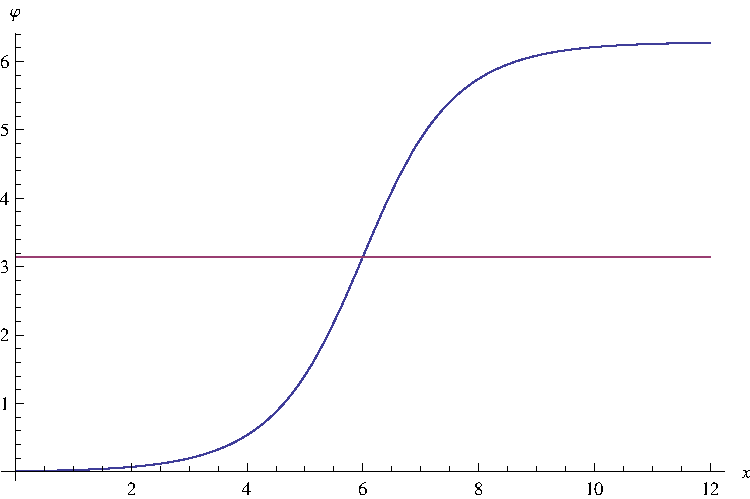
\includegraphics[width=0.47\linewidth,height=0.28\linewidth,clip]{./Bilder_SRT/Soliton_phi} \hspace{0.3cm}
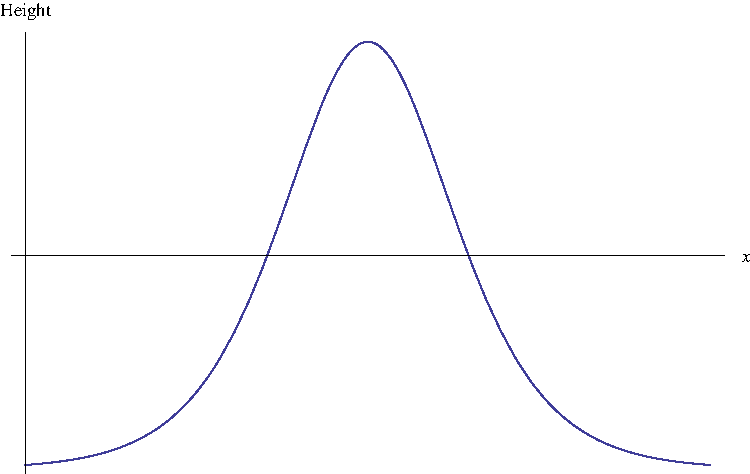
\includegraphics[width=0.47\linewidth,height=0.28\linewidth,clip]{./Bilder_SRT/Soliton_Height}%\\[0.5cm]
%\hspace*{3cm}\includegraphics[width=0.5\linewidth,height=0.3\linewidth,clip]{./Bilder_SRT/Soliton_3D}
\caption[]{ \label{fig:Soliton}
Die Soliton-L\"osung: (oben links) Der Auslenkungswinkel $\varphi$ 
als Funktion der Koordinate $x$ entlang der Aufh\"angung,
(oben rechts) die Seitenansicht.}
% (unten) die dreidimensionale Ansicht.}
\end{figure}

Die Soliton-L\"osung entspricht einer Konfiguration, bei der sich die
Pendel in der N\"ahe eines Punktes einmal um ihre Aufh\"angung herumwinden, 
sich anderenfalls aber im Wesentlichen in der
senkrecht herabh\"angenden Ruhelage befinden (siehe Abb.\ \ref{fig:Soliton}). 
Diese L\"osung ist stabil. 
Die statische L\"{o}sung des Kontinuumsmodells ist durch
\index{Soliton}
\begin{equation}
\label{soliton}
      \varphi_0(x) ~=~ 4 \tan^{-1}
      \left( \exp \pm \sqrt{g}(x-x_0) \right) 
\end{equation}
gegeben, wobei die Integrationskonstante $x_0$ die Position
des Solitons angibt, d.h.\ den Punkt, bei dem $\varphi=\pi$. 
Das + Zeichen in (\ref{soliton}) entspricht einer L\"osung, f\"ur die
$\lim_{x\rightarrow -\infty} \varphi(x) \rightarrow 0$ und
$\lim_{x\rightarrow +\infty} \varphi(x) \rightarrow 2\pi$. Das $-$ 
Zeichen beschreibt eine so\-ge\-nann\-te Anti-Soliton-L\"osung mit
$\lim_{x\rightarrow -\infty} \varphi(x) \rightarrow 2\pi$ und
$\lim_{x\rightarrow +\infty} \varphi(x) \rightarrow 0$.
In beiden F\"allen n\"ahern sich die L\"osungen ihrem asymptotischen Wert
f\"ur gro\ss e $|x-x_0|$ exponentiell. Die Reichweite der L\"osung 
entspricht dabei
\begin{equation}
\label{width}
   \Delta L ~=~ 1/\sqrt{g}   \;.
\end{equation}
Diese Gr\"o\ss e ist ein Ma\ss\ f\"ur die halbe Breite des Solitons und
soll uns als L\"angenskala dienen. 

\begin{figure}[htbp]
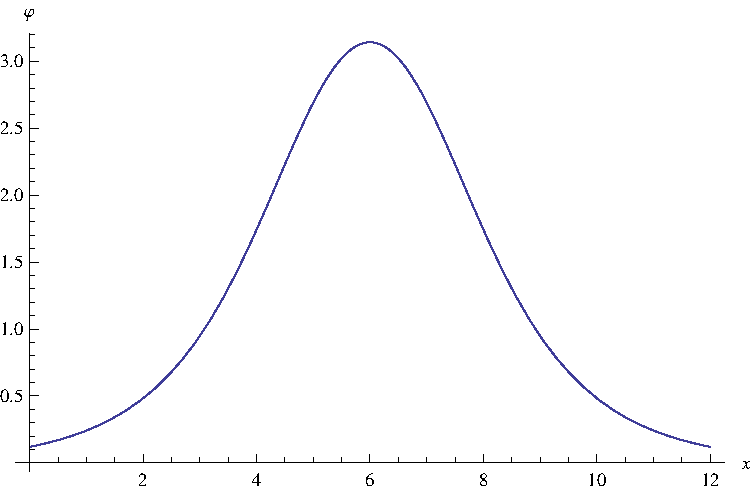
\includegraphics[width=0.47\linewidth,height=0.28\linewidth,clip]{./Bilder_SRT/Breather_phi} \hspace{0.3cm}
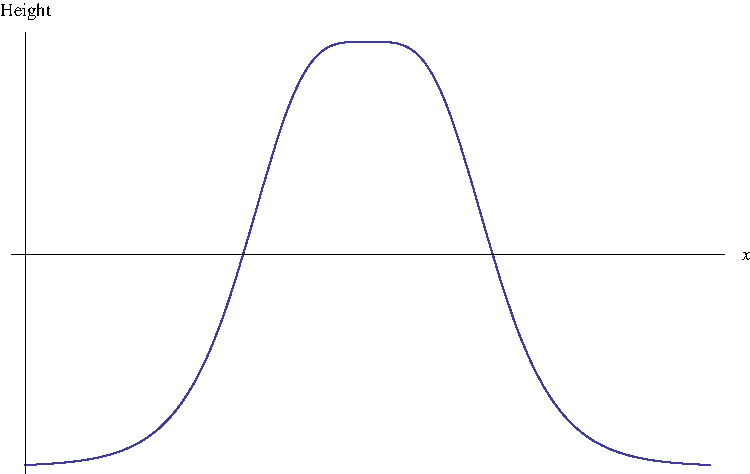
\includegraphics[width=0.47\linewidth,height=0.28\linewidth,clip]{./Bilder_SRT/Breather_Height}%\\[0.5cm]
%\hspace*{3cm}\includegraphics[width=0.5\linewidth,height=0.3\linewidth,clip]{./Bilder_SRT/Breather_3D}
\caption[]{ \label{fig:Breather}
Die Breather-L\"osung: (oben links) Der Auslenkungswinkel $\varphi$ 
als Funktion der Koordinate $x$ entlang der Aufh\"angung im
Augenblick maximaler Auslenkung,
(oben rechts) die Seitenansicht.}
%, (unten) die dreidimensionale Ansicht.}
\end{figure}

Die Sinus-Gordon Theorie besitzt ebenfalls L\"osungen, die gebundenen
Zust\"anden eines Solitons und eines Anti-Solitons entsprechen, die 
sogenannten Breather-L\"osungen (vgl.\ \cite{Lamb}; Darstellung in
Abb.\ \ref{fig:Breather}):
\index{Breather-L\"osung}
\begin{equation}
\label{breather}
    \varphi_0(x,t) ~=~ - 4 \tan^{-1} \left[ \frac{m}{\sqrt{1-m^2}}
    \frac{\sin \sqrt{g(1-m^2)}(t-t_0)}{\cosh m \sqrt{g}(x-x_0)} \right]\;.
\end{equation}
Der Parameter $m$ muss der Bedingung $0<m^2<1$ gen\"ugen, ist ansonsten 
aber beliebig. Die Schwingungsperiode ist
\begin{equation}
\label{time}
     \Delta T ~=~ \frac{2\pi}{\sqrt{g(1-m^2)}}~.
\end{equation}
Diese L\"osung ist metastabil. Es handelt sich um einen gebundenen
Zustand zwi\-schen einem Teilchen und seinem Antiteilchen, und kleine
St\"orungen lassen dieses System in \glqq Photonen\grqq\ zerfallen, d.h.\
einfache Schwingungen der Pendelkette. Der freie
Parameter $m$ h\"angt mit der Bindungsenergie zusammen und legt sowohl die
Amplitude als auch die Periode fest. Zur Festlegung einer Zeitskala
muss daher ein spezieller Wert f\"ur $m$ gew\"ahlt werden. Eine m\"ogliche
Wahl w\"are, dass $\varphi$ zwischen $-\pi$ und $+\pi$ variiert, d.h.\
$m^2=1/2$ oder $\Delta T=\sqrt{8\pi^2/g}$. (Dieser Wert f\"ur $m$ wurde
in Abb.\ \ref{fig:Breather} gew\"ahlt.)
\vspace{0.3cm}

Wir wollen nun untersuchen, wie sich die so definierten L\"angen-
und Zeitma\ss st\"abe transformieren, wenn man sie relativ zum
\glqq \"Ather\grqq, d.h.\ dem durch die Pendel definierten Ruhesystem,
bewegt.
Wir betrachten zun\"achst ein Soliton mit einer Geschwindigkeit
$v$. Diese L\"osung erhalten wir aus der statischen L\"osung nach 
Gleichung (\ref{eq_inv}). Auch die Breite des propagierenden Solitons
l\"asst sich daraus ablesen. 

Die statische L\"osung $\varphi_0(x)$ habe ihr Zentrum bei $x=0$. Dann
bestimmt die Bedingung
\[         \varphi_0(\pm \Delta L) ~=~ \pi \pm \alpha   \]
einen Wert f\"ur $\alpha$, bei dem wir die Breite von $\varphi_0$ messen.
F\"ur die propagierende L\"osung
\[         \varphi_v(x,t) ~=~ \varphi_0(\,\gamma(v)(x-vt)\,) \;,  \]
bewegt sich das Zentrum $x_0(t)$ nach der Gleichung $x_0(t)=vt$. Die
Breite dieser L\"osung ist gleich dem Wert $\Delta L_v$, der der
Bedingung
\[    \varphi_v(x_0(t)\pm \Delta L_v,t) ~=~ \pi \pm \alpha  \]
gen\"ugt. Dies ist offensichtlich der Fall f\"{u}r
\begin{equation}
\label{Lorentz}
        \gamma(v)\, \Delta L_v ~=~ \Delta L ~~~{\rm oder} ~~~
        \Delta L_v ~=~ \sqrt{1-v^2} \Delta L \;.  
\end{equation}
Die Breite der propagierenden L\"{o}sung ist daher um einen Faktor
$1/\gamma(v)$ kontrahiert. Diese \glqq Lorentz-Kontraktion\grqq\ kann von
\index{Lorentz-Fitzgerald-Kontraktion}
einem au\ss enstehenden Beobachter, der sieht, wie sich die Solitonen
entlang der Pendelkette ausbreiten, tats\"achlich wahrgenommen werden.

\begin{figure}[htbp]
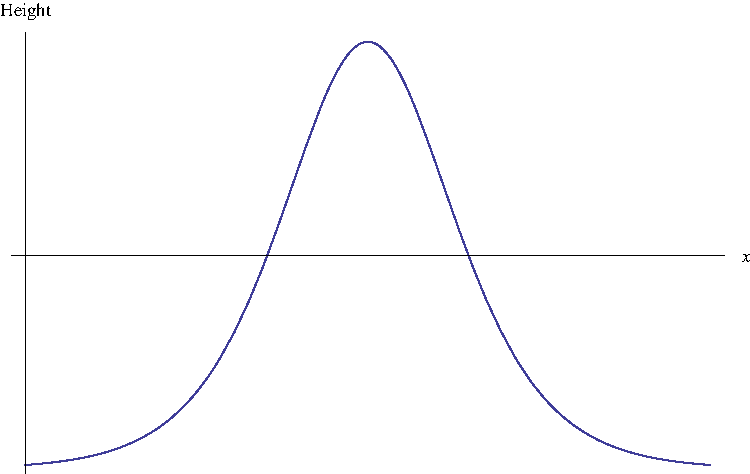
\includegraphics[width=0.47\linewidth,height=0.28\linewidth,clip]{./Bilder_SRT/Soliton_Height} \hspace{0.3cm}
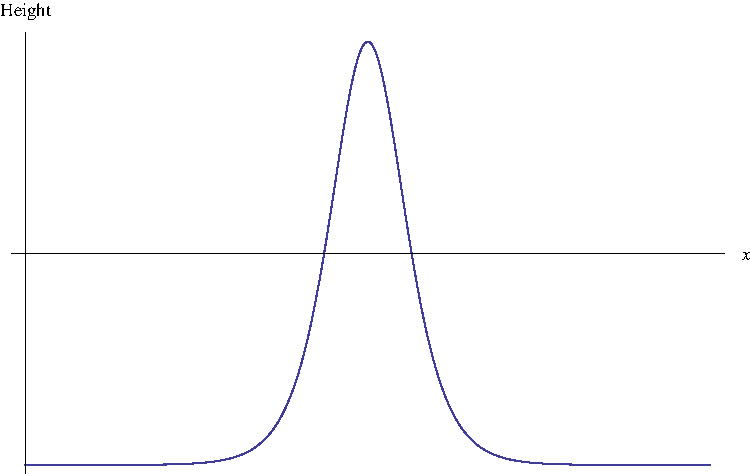
\includegraphics[width=0.47\linewidth,height=0.28\linewidth,clip]{./Bilder_SRT/Soliton_v09}
\begin{picture}(0,0)(0,0)
\thicklines
\put(-90,100){\vector(1,0){20}}
\put(-80,110){\makebox(0,0){$v=0{,}9$}}
\put(-280,110){\makebox(0,0){$v=0$}}
\end{picture}
\caption[]{ \label{fig:Soliton_v09}
Die Soliton-L\"osung in Bewegung: (links) Die ruhende 
Soliton-L\"osung aus Abb.\ \ref{fig:Soliton}, (rechts) 
die zugeh\"orige transformierte L\"osung zu einer 
Geschwindigkeit $v=0{,}9$.}
\end{figure}

Auch die Dilatation der Schwingungsperiode des gebundenen Zustands l\"asst
sich leicht herleiten. In Ruhe gilt f\"{u}r die Breather-L\"osung:
\[      \varphi_0^b(x,t) ~=~ \varphi_0^b(x,t+\Delta T) \;. \]
Die zugeh\"orige propagierende L\"osung erf\"ullt
\[   \varphi_v^b(x,t) ~=~ \varphi_v^b(x+v\Delta T_v, t+\Delta T_v) \;. \]
Da
\[   \varphi_v^b(x,t) ~=~
     \varphi_0^b \left(\,\gamma(v)(x-vt)\:,\:\gamma(v)(t-vx)\,\right)  \]
erhalten wir
\[   \gamma(v) \left( t+ \Delta T_v - v
     \left( x + v \Delta T_v \right) \right) ~=~
     \gamma(v) \left(t-v x \right) +
     \gamma(v) \left( 1-v^2\right) \Delta T_v \]
und somit:
\begin{equation}
\label{dilation}
      \Delta T ~=~ \gamma(v) \left(1-v^2 \right) \Delta T_v
      ~~~{\rm oder}~~~
      \Delta T_v ~=~ \frac{1}{\sqrt{1-v^2}} \Delta T \;.
\end{equation}
Die Schwingungsdauer eines sich bewegenden gebundenen Zustands ist
also tats\"achlich um einen Faktor $\gamma(v)$ im Vergleich zum ruhenden
Zustand verl\"angert.

Solitonen und gebundene Zust\"{a}nde von Solitonen k\"onnen an einem
festen Ende der Kette ohne Energieverlust reflektiert werden. Durch
eine solche experimentelle Anordnung kann man das 
\index{Zwillingsparadoxon}
\glqq Zwillingsparadoxon\grqq\ aufzeigen (vgl.\ Abschnitt \ref{chap_Zwilling}): 
Ein gebundener Zustand, der
sich entlang der Kette bewegt und nach einer Reflektion am Ende
der Kette zur\"uckkehrt, hat weniger Schwingungen ausgef\"uhrt, als ein
ruhender gebundener Zustand. Offensichtlich kann dieser Effekt
nicht der \glqq Beschleunigung\grqq\ am Ende der Kette
zugeschrieben werden.

\section{Von der \"Atherhypothese zur Relativit\"atstheorie}

Zun\"achst hat es vielleicht den Anschein, als ob das oben diskutierte
Modell der harmonisch gekoppelten Pendel sehr speziell sei. 
Hinsichtlich der Existenz von Soliton- und Breather-L\"osung mag das
richtig sein, nicht aber hinsichtlich der Tatsache, dass
dieses Modell den richtigen Verk\"urzungsfaktor und die richtige
Zeitdilatation liefert. Das einzige, was wir zur Herleitung dieser
Faktoren benutzt haben, ist die Lorentz-Invarianz der Feldgleichungen.
{\em Jede Lorentz-invariante Feldgleichung hat somit die Eigenschaft, dass
ihre L\"osungen, die eine L\"angen- oder Zeitskala definieren, sich genau
so transformieren, dass die bewegten Ma\ss st\"abe bzw.\ Uhren 
mit dem Lorentz'schen Verk\"urzungs- bzw.\ Dilatationsfaktor
multipliziert werden.}

Insbesondere haben auch die Maxwell-Gleichungen diese Eigenschaft.
Genau das hatte Lorentz gezeigt, wobei er allerdings noch die
falschen Transformationsgesetze f\"ur die Ladungen und Str\"ome
verwendet hatte. Diesen Fehler hat Poincar\'e korrigiert. Unter der 
Annahme, dass auf atomarer Ebene die 
Materie, und damit auch L\"angenma\ss st\"abe, durch die 
elektromagnetische Wechselwirkung zusammengehalten 
wird, war daher
die Lorentz-Kontraktion nicht nur plausibel sondern sogar eine
Folgerung aus den Maxwell-Gleichungen. 

Vor diesem Hintergrund k\"onnen wir auch den \"Ubergang
von der Lorentz'schen Sichtweise zur 
Einstein'schen Sichtweise und der 
speziellen Relativit\"atstheorie leichter nachvollziehen. 
Aus der Lorentz-Invarianz der fundamentalen Gleichungen
folgen ja nicht nur die Lorentz-Kontraktion und die Zeitdilatation,
sondern s\"amtliche Ph\"anomene, die sich im Rahmen der speziellen
Relativit\"atstheorie erkl\"aren lassen.

Oftmals wird behauptet, der \"Ubergang zur 
Sichtweise der speziellen Relativit\"atstheorie 
best\"unde in einer Neuinterpretation von 
\glqq Raum\grqq\ und \glqq Zeit\grqq.
Doch \"uber Raum und Zeit als abstrakte Entit\"aten 
k\"onnen wir eigentlich nichts sagen. In der Physik
interessieren wir uns nur f\"ur r\"aumliche und zeitliche
{\em Distanzen}, und diese Distanzen messen wir mir
physikalischen Instrumenten -- L\"angenma\ss st\"aben
und Uhren --, die selbst den physikalischen Gesetzen
unterliegen. 

Bisher bezog sich das Symbol $x$ auf 
eine Koordinate im Ruhesystem des
\"Athers -- im obigen Modell war dies das 
Ruhesystem der Pendelaufh\"angung. 
Dies entspricht dem \glqq Lineal\grqq\ eines 
externen Beobachters, der au\ss erhalb
unserer Welt steht und alles mit 
seinen Ma\ss st\"aben ausmessen kann -- 
wie wir bei den gekoppelten Pendeln. Entsprechend 
bezog sich auch das Symbol $t$ auf die Uhr eines externen Beobachters. Wir als
externe Beobachter k\"onnen die L\"angenkontraktion der Solitonen 
nachweisen, indem wir einfach ein \glqq externes\grqq\ 
Lineal neben das Soliton halten. Ebenso 
k\"onnen wir den propagierenden gebundenen Zustand beobachten und die 
Dilatation in der Schwingungsperiode 
mit unserer externen Uhr vergleichen. F\"ur uns als externe
Beobachter sind Raum (gemessen entlang der Pendelkette) und Zeit absolut. 
$c=1$ (die Geschwindigkeit von Wellen bzw.\ kleinen St\"orungen entlang der
Kette) ist f\"ur uns keine obere Grenzgeschwindigkeit, und wenn wir uns
entlang der Kette bewegen, ist die Ausbreitungsgeschwindigkeit einer
St\"orung entlang der Kette (das entspricht der Ausbreitung des Lichts)
in unserem System f\"{u}r die Vorw\"arts- und
R\"uckw\"artsrichtung verschieden: Das Ruhesystem der Pendelkette ist ein
ausgezeichnetes System.

Stellen wir uns nun jedoch (1+1)-dimensionale Wesen vor, die in dieser
\glqq Soliton-Welt\grqq\ leben. Ihnen stehen nur die Solitonen bzw.\ andere 
L\"osungen ihrer \glqq universellen Be\-we\-gungs\-glei\-chungen\grqq\ 
als L\"angen- und Zeitma\ss st\"abe zur Verf\"{u}gung. Sie werden daher
die Breite eines Solitons und die Schwingungsdauer der Breather-L\"osung
als L\"angen- und Zeitma\ss stab zur Beschreibung der physikalischen
Ph\"anomene benutzen. Doch wenn sie ein bewegtes Soliton mit
der Breite eines anderen bewegten Solitions vergleichen, \glqq messen\grqq\
sie keine Verk\"urzung, entsprechend messen sie auch mit
bewegten Breather-L\"osungen keine Ver\"anderungen in der
Zeitskala eines entsprechend bewegten Systems. Erst wenn sie
die Breite oder Zeitskalen von bewegten Systemen mit denen
von anders bewegten oder ruhenden Systemen vergleichen,
messen sie Unterschiede.

Der \"Ubergang zur Minkowski-Welt erfolgt gerade 
dadurch, dass die externen L\"angen- und Zeitma\ss st\"abe 
durch interne L\"angen- und Zeitma\ss st\"abe, die
denselben physikalischen Gesetzen unterliegen,
ersetzt werden. Es ist der \"Ubergang von
einer externen zu einer internen Perspektive.
Die zugrundeliegende diskrete Struktur 
und damit das ausgezeichnete Ruhesystem (der \glqq \"Ather\grqq) zeigen sich 
erst, wenn $v$ so gro\ss\ wird, dass die Brei\-te der Solitonen mit der 
Gr\"o\ss enordnung des 
Pendelabstands (bzw.\ der Gitterstruktur) vergleichbar wird. Ist die
fundamentale Theorie eine Kontinuumstheorie, 
so tritt der \glqq \"Ather\grqq\ 
f\"ur einen internen Beobachter \"uberhaupt nicht in Erscheinung.

Wenn wir von der Lorentz-Invarianz bzw.\ allgemeiner Poincar\'e-Invarianz
\index{Lorentz-Invarianz}
der Raum-Zeit sprechen, sollten wir eigentlich zwei Schritte bzw.\
Aspekte unterscheiden. Wir haben oben die Invarianzeigenschaft der
Bewegungsgleichungen als eine Eigenschaft der L\"osungsmenge dieser
Gleichungen interpretiert: Mit jeder L\"osung
$\varphi(x)$ ist auch $\varphi^{(\Lambda,a)}(x)=\varphi(\Lambda x -a)$  
eine L\"osung der Bewegungsgleichung. Gibt es nun ausgezeichnete
L\"osungen, die L\"angenma\ss st\"abe oder Uhren definieren, so bedeutet
diese Invarianz, dass bewegte L\"angenma\ss st\"abe k\"urzer, bewegte
Uhren langsamer erscheinen. Dies gilt zun\"achst bez\"uglich der
festen \glqq Hintergrunds-Raum-Zeit\grqq. Diesen Schritt hatte auch Lorentz
erkannt. Der wesentliche zweite Schritt aber blieb Einstein vorbehalten.
Er erkannte n\"amlich, dass die Poincar\'e-Invarianz einer Gleichung
auch bedeutet, dass bez\"uglich der intrinsischen Ma\ss st\"abe
das Relativit\"atsprinzip gilt und damit kein Inertialsystem
mehr ausgezeichnet ist. 

Statt die Lorentz-Invarianz der Gleichungen als Eigenschaft der
L\"osungsmenge anzusehen, was beispielsweise auch f\"ur die diskretisierte
Pendelkette einfach zu interpretieren war, k\"onnen wir die 
Lorentz-Invarianz auch als eine Freiheit der Koordinatenwahl auffassen.
Wenn wir n\"amlich die Raum- und Zeitkoordinaten einer 
Lorentz-Transformation unterwerfen, f\"ur eine Raumdimension somit
die Ersetzung
\begin{equation}
\label{LT}
   x \rightarrow x' ~=~ \frac{x - vt}{\sqrt{1-\beta^2}}  
    \hspace{0.5cm} {\rm und} ~~
    t \rightarrow t' ~=~ \frac{t - \frac{v}{c^2}x}{\sqrt{1-\beta^2}}
    \hspace{1cm} \left(\beta = \frac{v}{c} \right)  
\end{equation}    
vornehmen,
dann bleiben die Feldgleichungen unver\"andert. Ordnen wir nun die
Koordinaten $(x,t)$ bzw.\ $(x',t')$ jeweils Beobachtern zu, deren Weltlinie 
durch $x=0$ bzw.\ $x'=0$ und deren 
\glqq gleichzeitige Ereignisse\grqq\ 
durch die Bedingungen $t=$const.\ bzw.\ $t'=$const.\ definiert sind,
dann bedeutet die Invarianz der Feldgleichungen, dass beide Beobachter
dieselbe Physik sehen, d.h., es gilt das Relativit\"atsprinzip.  

Die Lorentz-Invarianz der Bewegungsgleichungen k\"onnen wir
offensichtlich physikalisch auf zwei vollkommen unterschiedliche Weisen
interpretieren. Einmal als Eigenschaft der L\"osungsmenge, die es uns
erlaubt, aus bestimmten L\"osungen andere zu gewinnen. Diese 
Interpretation bezieht alles auf einen festen Satz von Koordinaten $(x,t)$
(vgl.~(\ref{eq_inv})), der als das Koordinatensystem eines ausgezeichneten
Ruhesystems interpretiert werden kann. Bez\"uglich dieser Koordinaten
beobachten wir die Lorentz-Kontraktion und die Zeitdilatation. 

Die andere Interpretation impliziert das Relativit\"atsprinzip. Wenn
sich zwei Beobachter relativ zueinander mit einer konstanten 
Geschwindigkeit $v$ bewegen, k\"onnen sie unterschiedliche
Koordinatensysteme verwenden, in denen sie sich jeweils im
Ursprung (und damit in Ruhe) befinden. Jeder verwendet zur
Angabe von r\"aumlichen und zeitlichen Distanzen Werte, die mit 
Instrumenten in seinem System gemessen wurden. 
Die von den beiden Beobachtern verwendeten 
Koordinaten h\"angen \"uber die Gleichungen
(\ref{LT}) miteinander zusammen. In diesem Fall erfahren beide
Beobachter dieselbe Physik. In dieser Interpretation gibt es kein
ausgezeichnetes Ruhesystem -- der \"Ather ist verschwunden. 
Der Preis ist eine neue Vorstellung von Gleichzeitigkeit. Dieser letzte
Schritt zeichnete Einstein vor Lorentz und Poincar\'e aus. 
      
\section{Die Synchronisation von Uhren}
\label{sec_Synch}

Ein ungewohnter (und in manchen Kreisen immer noch umstrittener) Aspekt der speziellen
Relativit\"atstheorie ist ihr Konzept von Gleichzeitigkeit. 
Dabei wird\index{Gleichzeitigkeit}
oft vergessen, dass es sich bei der Behauptung, zwei 
Ereignisse seien gleichzeitig, nicht um eine
\glqq faktische\grqq\ Aussagen handelt, sondern 
eher um eine Konvention.\footnote{Versteht man unter \glqq faktisch\grqq, dass
sich alle Beobachter unabhh\"angig von ihrem Bezugssystem in einer Aussage
einig sind, so ist die Gleichzeitigkeit in der Newton'schen Physik faktisch, in der
Relativit\"atstheorie jedoch nicht.}
Ob zwei Ereignisse f\"ur ein gegebenes Inertialsys\-tem gleichzeitig
stattfinden oder
nicht, k\"onnen wir experimentell nur entscheiden, wenn wir eine
Vorschrift angeben, was wir unter \glqq gleichzeitig\grqq\ verstehen
wollen. Diese Vorschrift wird letztendlich darin bestehen, dass wir
zwei Ereignisse als gleichzeitig ansehen, wenn die Uhren
am jeweiligen Ort dieser Ereignisse dieselbe Zeit anzeigen, womit wir das
Problem auf die Synchronisation von Uhren an verschiedenen
Orten (aber im selben Inertialsystem) reduzieren haben. 
Die einzige Einschr\"ankung ist, dass zwei gleichzeitige 
Ereignisse $A$ und $B$ {\em nicht} in einer kausalen Abh\"angigkeit stehen 
sollten. Grunds\"atzlich k\"onnen wir
eine beliebige raumartige Hyperfl\"ache als gleichzeitig {\em definieren}.

Die folgenden \"Uberlegungen gelten f\"ur den flachen Minkowski-Raum.
Wir konzentrieren uns ausschlie\ss lich auf den Aspekt der
Synchronisation\index{Synchronisation von Uhren} 
von Uhren f\"ur ein gegebenes Inertialsystem. Eine
ausf\"uhrlichere Darstellung dieser Problematik findet man bei 
Mittelstaedt \cite{Mittelstaedt} sowie in den beiden Abhandlungen
{\em Philosophie der Raum-Zeit-Lehre} \cite{Reichenbach1} und 
{\em Axiomatik der relativistischen Raum-Zeit-Lehre} \cite{Reichenbach2}
von Hans Reichenbach\index{Reichenbach, Hans} 
(Hans Friedrich Herbert G\"unther Reichenbach,
{\em geb.\ 26.9.1891 in Hamburg; gest.\ 9.4.1953 in Los Angeles}). 

\subsection{Synchronisation durch Lichtsignale}

Zun\"achst ist es recht hilfreich, sich bei der operationalen
Definition von Gleichzeitigkeit auf ein 
allgemeines Verfahren zu beschr\"anken, das allerdings
noch keine Einschr\"ankung an die M\"oglichkeiten darstellt. 
Wir wollen Uhren durch
Austausch von Lichtsignalen synchronisieren. Beobachter $A$ sendet zum
Zeitpunkt $t_1$ ein Lichtsignal aus. Dieses wird von Beobachter $B$
reflektiert und erreicht Beobachter $A$ zum Zeitpunkt $t_2$. Bezeichnen
wir den Zeitpunkt des Ereignisses der Reflektion des Lichtstrahls bei
Beobachter $B$ mit $t$, so m\"ochte Beobachter
$A$ nun definieren, welches Ereignis auf seiner Weltlinie zu
dem Moment der Reflektion des Lichtstrahls bei Beobachter $B$ gleichzeitig
war, d.h.\ dem Zeitpunkt $t$ entspricht. Die einzige Einschr\"ankung
liefert dabei die Forderung der Kausalit\"at: $t_1 < t < t_2$. Beobachter
$A$ definiert nun:
\[      t ~=~ t_1 + \epsilon(A,B) (t_2 - t_1)     \]
mit 
\[         0 < \epsilon(A,B) < 1  \;.   \]
(Der Einfachheit halber soll das Synchronisierungsverfahren nicht von
der Zeit abh\"angen, d.h.\ $\epsilon(A,B)$ h\"angt nicht zus\"atzlich
noch von $t$ bzw.\ $t_1$ ab.)   

\begin{SCfigure}[50][htb]
\begin{picture}(120,200)(0,0)
\put(20,20){\line(0,1){180}}
\put(80,20){\line(0,1){180}}
\put(20,50){\line(1,1){60}}
\put(20,170){\line(1,-1){60}}
\put(20,80){\line(2,1){60}}
\put(20,10){\makebox{$A$}}
\put(80,10){\makebox{$B$}}
\put(50,0){\makebox{(a)}}
\put(10,50){\makebox{$t_1$}}
\put(10,170){\makebox{$t_2$}}
\put(6,78){\makebox{$x_A$}}
\put(84,108){\makebox{$x_B$}}
\end{picture}
%
\begin{picture}(100,200)(0,0)
\put(20,20){\line(0,1){180}}
\put(80,20){\line(0,1){180}}
\put(20,70){\line(1,1){60}}
\put(20,190){\line(1,-1){60}}
\put(20,100){\line(2,1){60}}
\put(20,100){\line(1,1){60}}
\put(20,100){\line(1,-1){60}}
\put(20,10){\makebox{$A$}}
\put(80,10){\makebox{$B$}}
\put(50,0){\makebox{(b)}}
\put(10,70){\makebox{$t_1$}}
\put(10,190){\makebox{$t_2$}}
\put(7,98){\makebox{$x_A$}}
\put(84,128){\makebox{$x_B$}}
\put(84,40){\makebox{$t'_1$}}
\put(84,160){\makebox{$t'_2$}}
\end{picture}
\caption{\label{figsyn}%
Synchronisation von Uhren durch Lichtstrahlen. Die senkrechten Linien
entsprechen den Weltlinien der Beobachter $A$ und $B$, die zueinander
einen konstanten Abstand halten. (a) Zum Zeitpunkt $t_1$ sendet $A$ ein
Lichtsignal aus, das von $B$ im Ereignis $x_B$ reflektiert wird und
bei $t_2$ wieder Beobachter $A$ erreicht. Durch Vorgabe von $\epsilon_A$
konstruiert $A$ das Ereignis $x_A$, das zu $x_B$ gleichzeitig ist.
(b) Soll die Gleichzeitigkeit der Ereignisse $x_A$ und $x_B$ auch f\"ur
Beobachter $B$ gelten, so muss er sein Verfahren zur Bestimmung der
Gleichzeitigkeit (ausgedr\"uckt durch $\epsilon_B$) so w\"ahlen, 
dass $\epsilon_B=1-\epsilon_A$.} 
\end{SCfigure}

Zun\"achst kann man sich leicht \"uberzeugen, dass durch geeignete 
Wahl von $\epsilon$ tats\"achlich je zwei raumartige Ereignisse $x_A$ und
$x_B$ auf der Weltlinie von $A$ und $B$ als gleichzeitig 
definiert werden k\"onnen (vgl.\ Abb.~\ref{figsyn}). 
Dieses Verfahren bildet daher keine Einschr\"ankung der Allgemeinheit. 
Damit die Hyperfl\"ache der zu $x_A$ gleichzeitigen Ereignisse eine
raumartige Hyperfl\"ache ist, m\"ussen die Richtungsableitungen der 
Funktion $\epsilon(A,B)$ (aufgefasst als eine Funktion von $B$) noch
durch eine Konstante (bei unserer Definition der Lichtgeschwindigkeit
ist diese Konstante 1) beschr\"ankt sein. Durch geeignete Forderungen
an die Funktion $\epsilon$ erh\"alt man verschiedene 
Synchronisationsverfahren.

\subsection{Die Einstein-Synchronisation}

Eine sehr allgemeine Forderung an die Gleichzeitigkeit von Ereignissen
\index{Symmetrie der Gleichzeitigkeit}
ist die Symmetrieforderung: Wenn f\"ur einen Beobachter $A$ das 
Ereignis $x_B$ auf der Weltlinie eines Beobachters $B$ gleichzeitig zu
dem Ereignis $x_A$ auf seiner Weltlinie ist, dann soll umgekehrt auch
f\"ur den Beobachter $B$ das Ereignis $x_A$ gleichzeitig zu $x_B$ sein.
Anhand der Abbildung \ref{figsyn}(b) kann man sich leicht \"uberzeugen,
dass diese Forderung gleichbedeutend mit der Bedingung
\[          \epsilon(A,B) ~=~ 1 - \epsilon(B,A)      \]
ist. 

Eine weitere allgemeine Forderung ergibt sich aus der Homogenit\"at des
\index{Homogenit\"at des Raumes}
Raumes. Wir verlangen, dass sich die Funktion $\epsilon(A,B)$ nicht
\"andert, wenn wir die beiden Beobachter $A$ und $B$ um {\em denselben}
(r\"aumlichen) Vektor verschieben. Symbolisch ausgedr\"uckt:
\[     \epsilon(A+\vec{a},B+\vec{a}) ~=~ \epsilon(A,B)     \;.  \]
Dies bedeutet, dass $\epsilon(A,B)$ nur noch von der r\"aumlichen 
Richtung abh\"angen kann, unter der der Beobachter $B$ von $A$ aus gesehen
wird. Innerhalb einer Halbebene, die die Weltlinie von $A$
als Rand hat, ist $\epsilon$ konstant. Auch diese Forderung verlangen
wir allgemein.

Nun kommen wir zu einer speziellen Forderung, die sich aus der Konstanz
der Lichtgeschwindigkeit ergibt. Da die Lichtgeschwindigkeit f\"ur jeden
Beobachter und f\"ur jede Richtung dieselbe sein soll, k\"onnen wir
zus\"atzlich noch Isotropie 
\index{Isotropie des Raumes}
unserer Gleichzeitigkeitsdefinition verlangen.
$\epsilon$ soll also auch nicht mehr von der r\"aumlichen Richtung 
abh\"angen, unter der $B$ von $A$ aus gesehen wird. In diesem Fall 
gilt
\[       \epsilon(A,B) ~=~ {\rm const}    \;.  \]
Zusammen mit der ersten Forderung der Symmetrie folgt sofort:
\[       \epsilon ~=~ \frac{1}{2}  \;.   \]
Die aus diesem Wert f\"ur $\epsilon$ folgende Synchronisation von
Uhren bezeichnet man als\index{Einstein-Synchronisation} 
Einstein-Synchronisation. 

Das zweite Axiom der speziellen Relativit\"atstheorie - die Konstanz
der Lichtgeschwindigkeit - f\"uhrt uns somit schon zur Festlegung der
Gleichzeitigkeitsvorschrift. Das erste Axiom - 
das Relativit\"atsprinzip\index{Relativit\"atsprinzip} -
geht indirekt in diese Festlegung ein, da wir die Konstanz der 
Lichtgeschwindigkeit und somit die Isotropie der
Synchronisationsvorschrift f\"ur jedes Inertialsystem verlangt haben. 
  
\subsection{Synchronisation mit der \"Atherhypothese}

Wir haben aus der Lorentz-Invarianz der universellen Bewegungsgleichungen
geschlossen, dass die spezielle Relativit\"atstheorie in der 
Formulierung von Einstein \"aquivalent zur Lorentz-Theorie ist, d.h.\
zu einer Theorie mit \"Atherhypothese und Lorentz-Kon\-traktion der
L\"angenskalen. Es sollte daher nicht \"uberraschen, wenn es eine
Synchronisationsvorschrift gibt, die auf die Lorentz-Theorie f\"uhrt.

\begin{figure}[ht]
\begin{picture}(360,200)(0,0)
\put(30,120){\vector(1,0){120}}
\put(80,10){\vector(0,1){170}}
\put(30,20){\line(1,2){80}}
\thicklines
\put(40,40){\line(1,1){80}}
\put(120,120){\line(-1,1){27}}
\thinlines
\put(80,120){\makebox(0,0){{\footnotesize $\bullet$}}}
\put(120,120){\makebox(0,0){{\footnotesize $\bullet$}}}
\put(40,40){\makebox(0,0){{\footnotesize $\bullet$}}}
\put(93,147){\makebox(0,0){{\footnotesize $\bullet$}}}
\put(75,125){\makebox(0,0){$O$}}
\put(32,40){\makebox(0,0){$A$}}
\put(87,150){\makebox(0,0){$B$}}
\put(123,128){\makebox(0,0){$C$}}
\put(75,180){\makebox(0,0){$t$}}
\put(150,115){\makebox(0,0){$x$}}
\put(100,10){\makebox(0,0){(a)}}
%
\put(210,120){\vector(1,0){120}}
\put(260,10){\vector(0,1){170}}
\put(210,20){\line(1,2){80}}
\put(220,80){\line(2,1){100}}
\thicklines
\put(220,40){\line(1,1){80}}
\put(300,120){\line(-1,1){27}}
\thinlines
\put(246.5,93){\makebox(0,0){{\footnotesize $\bullet$}}}
\put(300,120){\makebox(0,0){{\footnotesize $\bullet$}}}
\put(220,40){\makebox(0,0){{\footnotesize $\bullet$}}}
\put(273,147){\makebox(0,0){{\footnotesize $\bullet$}}}
\put(255,125){\makebox(0,0){$O$}}
\put(212,40){\makebox(0,0){$A$}}
\put(267,150){\makebox(0,0){$B$}}
\put(303,128){\makebox(0,0){$C$}}
\put(240,97){\makebox(0,0){$D$}}
\put(255,180){\makebox(0,0){$t$}}
\put(330,115){\makebox(0,0){$x$}}
\put(280,10){\makebox(0,0){(b)}}
\end{picture}
\caption{\label{figuhr}%
\"Ather- und Einstein-Synchronisation. In Teil (a) rekonstruiert der
Beobachter auf der Weltlinie $AB$ das Ereignis $O$ als gleichzeitig zum
Ereignis $C$. Seine Synchronisationsvorschrift h\"angt von der 
Geschwindigkeit $v$ relativ zu dem ausgezeichneteten Ruhesystem ab.
Dabei gilt f\"ur das Verh\"altnis $(AO)/(AB)=(1+v)/2$. 
In Abbildung (b) wird nach der Einstein-Synchronisation aus denselben
Lichtsignalen das Ereignis $D$ als zu $C$ gleichzeitig rekonstruiert.}
\end{figure}

Auch mit \"Atherhypothese verlangen wir von der Gleichzeitigkeit von
\index{Aetherhypothese@\"Atherhypothese}
Ereignissen Symmetrie und Homogenit\"at des Raumes. Was wir jedoch
nicht mehr verlangen k\"onnen, ist die allgemein g\"ultige Isotropie
der Synchronisationsvorschrift. F\"ur ein System, das sich relativ zum
\"Ather mit einer Geschwindigkeit $\vec{v}$ bewegt, wird die
Synchronisationsvorschrift von der Richtung relativ zu $\vec{v}$
abh\"angen. Allgemein wird also nun gelten:
\[         \epsilon(A,B) ~=~ \epsilon(\vec{v};A,B)   \;.   \]
Lediglich f\"ur das ausgezeichnete Inertialsystem, das dem
Ruhesystem des \"Athers entspricht, ist die Lichtgeschwindigkeit in
alle Richtungen dieselbe und somit das Synchronisationsverfahren
symmetrisch:
\[       \epsilon(\vec{v}=0;A,B) ~=~ \frac{1}{2}   \;.   \]
Bewegt sich das Inertialsystem der Beobachter $A$ und $B$ relativ
zum \"Ather mit der Geschwindigkeit $\vec{v}$, so gilt 
(vgl.\ Abb.~\ref{figuhr})
\[      \epsilon(\vec{v};A,B) ~=~ \frac{1}{2} 
        \left( 1 + \frac{|\vec{v}|}{c}\cos \alpha \right)  \;, \]
wobei $\alpha$ der Relativwinkel zwischen der Richtung von $\vec{v}$
und der Halbebene ist, die durch die Weltlinie
von $A$ begrenzt wird und die Weltlinie von $B$ enth\"alt.

Der Vorteil dieses Verfahrens ist, dass Gleichzeitigkeit nun
ein absoluter Begriff wird. Sind zwei Ereignisse $x_A$ und $x_B$
f\"ur einen Beobachter $A$ gleichzeitig, so sind sie es auch f\"ur
alle anderen Beobachter, unabh\"angig von deren Bewegungszustand.
 
Der Nachteil dieses Verfahrens ist jedoch, dass wir das Ruhesystem
des \"Athers nicht kennen. Wir m\"ussen also willk\"urlich ein System
auszeichnen, das wir als Ruhesys\-tem definieren, beispielsweise das
System des Schwerpunkts der in unserem Universum beobachtbaren Massen
oder das Ruhe\-sys\-tem relativ zur Hintergrundstrahlung. (Es ist nicht
selbstverst\"andlich, dass diese beiden Sys\-teme identisch sind.)
Wegen der Geschwindigkeitsabh\"angigkeit des Synchronisationsverfahrens
gilt das Relativit\"atsprinzip nicht mehr. Die Lichtgeschwindigkeit
ist nur im Ruhesystem des \"Athers richtungs\-un\-ab\-h\"angig konstant.

Das Relativit\"atsprinzip gilt jedoch in einer anderen Form:
Wir k\"onnen jedes beliebige Inertialsystem als Ruhesystem definieren
und die Synchronisation der Uhren auf dieses System beziehen. Die
physikalischen Gesetze bleiben dieselben. Hier liegt der physikalisch
unbefriedigende Aspekt dieses Synchronisierungsverfahrens. Wir brechen
die Symmetrie, die sich im Relativit\"atsprinzip ausdr\"uckt,
{\em per Hand}, indem wir ein Inertialsystem auszeichnen. Umgekehrt
tr\"agt die Einstein-Synchronisation dem Relativit\"atsprinzip Rechnung.
Kein Inertialsystem wird durch dieses Verfahren ausgezeichnet. Der
Preis ist allerdings die Relativit\"at der Gleichzeitigkeit.

Unter bestimmten Unst\"anden ist es jedoch sinnvoll, eine
Synchronisation zu w\"ahlen, die der Lorentz'schen Sichtweise
n\"aher ist als der Einstein'schen. Beispielsweise k\"onnte man
die Lorentz'sche Sichtweise so interpretieren, dass iregendwo in der Mitte
unseres Universums eine riesige Uhr steht, und das, was diese Uhr anzeigt,
ist die \glqq wahre\grqq\ Zeit. Alle anderen Systeme m\"ussen ihre Zeit auf
diese wahre Zeit umrechnen. Dieses Verfahren wird in abgewandelter Form
beispielsweise bei der Zeitsynchronisation des GPS-Satellitensystems verwendet.
Die \glqq riesige Uhr\grqq\ steht in der GPS-Zentrale in Colorado. Die 
Uhren der Satelliten sind so geschaltet, dass ihre Zeit gleich der 
\glqq Masterzeit\grqq\ ist. Insbesondere ist ihr Gang im 
Vergleich zu einer \glqq richtigen\grqq\
Uhr etwas gedrosselt, um den Einfluss der schw\"acheren Gravitation sowie
der Bewegung auszugleichen.

Die Einstein-Synchronisation wie auch die 
\glqq \"Athersynchronisation\grqq\
sind Spezialf\"alle einer Klasse von Synchronisationsvorschriften, bei
denen die Konstanz der sogenannten \glqq Zwei-Wege-Lichtgeschwindigkeit\grqq\
\index{Zwei-Wege-Lichtgeschwindigkeit}%
gefordert wird. Dabei handelt es sich um die Geschwindigkeit $c$, die
man einem Lichtstrahl zuordnet, der eine Strecke in beide Richtungen -
vor und zur\"uck - durchl\"auft. Ist $c^+$ die Geschwindigkeit f\"ur
eine Richtung und $c^-$ die Geschwindigkeit f\"ur die R\"uckrichtung,
so ist
\[   \frac{1}{c} ~=~ \frac{1}{2} \left( \frac{1}{c^+} + \frac{1}{c^-}
                  \right)   \;.    \]
W\"ahrend jedoch zur Messung von $c^+$ bzw.\ $c^-$ die Uhren an 
verschiedenen
Raumpunkten synchronisiert sein m\"ussen, kann man $c$ an einem Punkt
auswerten, d.h.\ $c$ h\"angt nicht von der Synchronisationsvorschrift
ab. Im Michelson-Morley-Versuch\index{Michelson-Morley-Experiment} 
beispielsweise wird die Lichtgeschwindigkeit
ja gar nicht f\"ur verschiedenen Raumrichtungen verglichen, sondern nur
die Zwei-Wege-Lichtgeschwindigkeit. Nur von dieser wird gezeigt, dass
sie isotrop ist. Die Einstein'sche Forderung der Konstanz der
Lichtgeschwindigkeit geht also \"uber das Ergebnis des 
Michelson-Morley-Versuchs hinaus.

\subsection{Synchronisation durch langsamen Uhrentransport} 

Abschlie\ss end soll noch gezeigt werden, dass die
Synchronisation durch langsamen Uhrentransport zu demselben
Ergebnis wie die Einstein-Synchronisation f\"uhrt. 
Das bedeutet Folgendes: Synchronisiert man zwei Uhren am selben Ort
und bringt dann die eine der beiden Uhren
langsam zu einem anderen Ort, ist die so
erreichte Synchronisation eine Einstein-Synchronisation.

Zun\"achst sollten wir etwas genauer definieren,
was \glqq Synchronisation durch langsamen Uhrentransport\grqq\
bedeutet. Wir stellen uns dazu zwei Beobachter vor, die
einen konstanten Abstand $L$ halten und sich im
selben Inertialsystem befinden. Zu einem Zeitpunkt $t_0=0$ werden bei
Beobachter 1 zwei Uhren synchronisiert. Anschlie\ss end
wird eine der beiden Uhren mit der Geschwindigkeit $v$
zu Beobachter 2 gebracht. Sie ben\"otigt dazu f\"ur 
Beobachter 1 die Zeit $t=L/v$, das ist also die Zeit,
die Beobachter 1 dem Ereignis \glqq Uhr ist bei Beobachter 
2\grqq\ zuschreiben wird. Die Anzeige auf
der Uhr ist allerdings nach der Relativit\"atstheorie etwas k\"urzer, n\"amlich
\begin{equation}
\label{eq_Korrektur}
           t_1 = \sqrt{1-\frac{v^2}{c^2}} t \, .  
\end{equation}
Wir k\"onnen nicht einfach argumentieren, dass
f\"ur $v/c\ll 1$ die rechte Seite gegen $t$ geht,
denn wenn $v$ sehr klein ist, wird $t$ sehr gro\ss,
und damit  w\"urde zwar $t_1/t$ gegen 1 gehen,
aber $t_1$ und $t$ k\"onnten sich m\"oglicherweise
selbst im Limes $v\rightarrow 0$ noch um einen konstanten
Term unterscheiden. Es gilt aber
\begin{equation}
       t_1 = \left( 1 - \frac{v^2}{c^2} + O((v/c)^4) \right) \frac{L}{v}
       \approx \frac{L}{v} - \frac{L}{c}\frac{v}{c} + ... 
       = t -  \frac{L}{c}\frac{v}{c} + ...
\end{equation} 
Da $L$ und $c$ Konstanten sind ($L/c$ ist die Zeit, die das
Licht braucht, die Strecke $L$ zu durchqueren), wird
der Korrekturterm f\"ur sehr kleine Geschwindigkeiten
beliebig klein. Allerdings ist die Korrektur von der
Ordnung $v/c$ und nicht, wie man zun\"achst nach
Gleichung \ref{eq_Korrektur} erwarten k\"onnte,
von der Ordnung $(v/c)^2$. 
 
\begin{thebibliography}{99}
\addcontentsline{toc}{chapter}{Literaturangaben}
\bibitem{Lamb} G.L.\ Lamb, Jr.; {\it Elements of Soliton Theory}; 
         Pure \& Applied Mathematics, John Wiley \& Sons, 1980. 
\bibitem{Mittelstaedt} Peter Mittelstaedt; {\it Der Zeitbegriff in der
        Physik}; BI-Wissenschaftsverlag, 1989.        
\bibitem{Reichenbach1} Hans Reichenbach; {\em Philosophie der 
       Raum-Zeit-Lehre}; Hans Reichenbach - Gesammelte Werke Bd.\ 2;
       Vieweg-Verlag, Braunschweig; 1977.
\bibitem{Reichenbach2} Hans Reichenbach; {\em Axiomatik der
       relativistischen Raum-Zeit-Lehre}; in {\em Die philosophische
       Bedeutung der Relativit\"atstheorie}; Hans Reichenbach - Gesammelte
       Werke Bd.\ 3; Vieweg-Verlag, Braunschweig, 1977. 
\end{thebibliography}
  
\end{document}

\documentclass[german,10pt]{book}    
\usepackage{makeidx}
\usepackage{babel}            % Sprachunterstuetzung
\usepackage{amsmath}          % AMS "Grundpaket"
\usepackage{amssymb,amsfonts,amsthm,amscd} 
\usepackage{mathrsfs}
\usepackage{rotating}
\usepackage{sidecap}
\usepackage{graphicx}
\usepackage{color}
\usepackage{fancybox}
\usepackage{tikz}
\usetikzlibrary{arrows,snakes,backgrounds}
\usepackage{hyperref}
\hypersetup{colorlinks=true,
                    linkcolor=blue,
                    filecolor=magenta,
                    urlcolor=cyan,
                    pdftitle={Overleaf Example},
                    pdfpagemode=FullScreen,}
%\newcommand{\hyperref}[1]{\ref{#1}}
%
\definecolor{Gray}{gray}{0.80}
\DeclareMathSymbol{,}{\mathord}{letters}{"3B}
%
\newcounter{num}
\renewcommand{\thenum}{\arabic{num}}
\newenvironment{anmerkungen}
   {\begin{list}{(\thenum)}{%
   \usecounter{num}%
   \leftmargin0pt
   \itemindent5pt
   \topsep0pt
   \labelwidth0pt}%
   }{\end{list}}
%
\renewcommand{\arraystretch}{1.15}                % in Formeln und Tabellen   
\renewcommand{\baselinestretch}{1.15}                 % 1.15 facher
                                                      % Zeilenabst.
\newcommand{\Anmerkung}[1]{{\begin{footnotesize}#1 \end{footnotesize}}\\[0.2cm]}
\newcommand{\comment}[1]{}
\setlength{\parindent}{0em}           % Nicht einruecken am Anfang der Zeile 

\setlength{\textwidth}{15.4cm}
\setlength{\textheight}{23.0cm}
\setlength{\oddsidemargin}{1.0mm} 
\setlength{\evensidemargin}{-6.5mm}
\setlength{\topmargin}{-10mm} 
\setlength{\headheight}{0mm}
\newcommand{\identity}{{\bf 1}}
%
\newcommand{\vs}{\vspace{0.3cm}}
\newcommand{\noi}{\noindent}
\newcommand{\leer}{}

\newcommand{\engl}[1]{[\textit{#1}]}
\parindent 1.2cm
\sloppy

    \begin{document} \setcounter{chapter}{3}

\chapter{SRT - Effekte}   %  Kap. 4
\label{chap_SRT-Effekte}

In diesem Kapitel sollen einige Effekte beschrieben werden, die sich
aus der Lorentz-Invarianz der Minkowski-Raumzeit ergeben.
Dazu z\"ahlen die Zeitdilatation, die Lorentz-Kontraktion und der relativistische
Doppler-Effekt (longitudinal und transversal). Dem sogenannten 
Zwillings-Paradoxon ist ein eigenes Kapitel gewidmet (Kap.\ \ref{chap_Zwilling}).

Anschlie\ss end deuten wir an, wie sich der Lagrange-Formalismus auf die
Relativit\"atstheorie verallgemeinern l\"asst und was der zum Ortsvektor
kanonisch konjugierte Impuls ist. In diesem Zusammenhang definieren wir
auch den Begriff der Eigenzeit. Den Abschluss bildet ein von Einstein
erdachtes Gedankenexeriment, das eine elegante Herleitung der 
bekannten Beziehung $E=mc^2$ erlaubt.

\section{Zeitdilatation}

Wir behandeln zun\"achst das Ph\"anomen
der Zeitdilatation. Schon bei der Pendelkette
hatten wir gesehen, dass aus der Lorentz-Invarianz
der Feldgleichungen folgt, dass eine
relativ zum \"Ather bewegte Breather-L\"osung
langsamer schwingt bzw.\ eine gr\"o\ss ere
Schwingungsperiode hat, als eine Breather-L\"osung, die relativ zum \"Ather ruht.  
Doch aus dem Relativit\"atsprinzip sollte folgen,
dass ein Beobachter in dem bewegten System
umgekehrt ebenfalls den Eindruck hat, dass
die Uhren in dem ruhenden System langsamer
gehen. Wir wollen nun untersuchen, was
genau damit gemeint ist und weshalb dieses
Ph\"anomen tats\"achlich auftritt. 

\begin{SCfigure}[50][htb]
\setlength{\unitlength}{2.1pt}
\begin{picture}(125,110)(0,0)
\put(20,35){\vector(1,0){95}}
\put(50,5){\vector(0,1){90}}
\put(35,5){\vector(1,2){45}}
%\qbezier(19,102.5)(85,35)(151,102.5)
\qbezier(50,68.5)(82,68.5)(116,102.5)
\qbezier(0,88)(28,68.5)(50,68.5)
\put(68,71){\makebox(0,0){{\footnotesize $\bullet$}}}
\put(50,68.5){\makebox(0,0){{\footnotesize $\bullet$}}}
\put(66.5,68.3){\makebox(0,0){{\footnotesize $\bullet$}}}
\put(50,62.4){\makebox(0,0){{\footnotesize $\bullet$}}}
\put(50,35){\makebox(0,0){{\footnotesize $\bullet$}}}
\put(69,65.5){\makebox(0,0){$B'$}}
\put(64,73){\makebox(0,0){$A'$}}
\put(47.5,71.5){\makebox(0,0){$A$}}
\put(56,33){\makebox(0,0){$O$}}
\put(52,60){\makebox(0,0){$B$}}
\put(15,45){\line(2,1){105}}
\put(20,68.5){\line(1,0){90}}
\put(16,18){\vector(2,1){100}}
\put(110,33){\makebox(0,0){$x$}}
\put(110,62){\makebox(0,0){$x'$}}
\put(48,90){\makebox(0,0){$t$}}
\put(81,90){\makebox(0,0){$t'$}}
\put(50,100){\makebox(0,0){$1$}}
\put(80,100){\makebox(0,0){$2$}}
\multiput(66.5,5)(0,8){12}{\line(0,1){6}}
\multiput(21.3,5)(4,8){12}{\line(1,2){3}}
\thicklines
\put(20,5){\line(1,1){95}}
\put(80,5){\line(-1,1){80}}
\end{picture}
\caption{\label{fig_zeitdilat}%
F\"ur den ruhenden Beobachter 1 scheint
die bewegte Uhr von Beobachter 2 langsamer zu gehen
($B'$ liegt vor $A'$). Denselben
Eindruck hat umgekehrt auch der 
Beobachter 2 von der Uhr von Beobachter 1 ($B$ liegt vor $A$).
Die gestrichelten Linien beziehen sich auf jeweils einen
weiteren Beobachter in System 1 bzw.\ System 2. Diese
Beobachter lesen ihre (mit 1 bzw.\ 2 synchronosierten) Uhren bei den
Ereignissen $B'$ und $B$ ab.}
\end{SCfigure}

Wir betrachten wieder zwei Inertialsysteme
mit den jeweiligen Koordinaten $(x,t)$ und
$(x',t')$ (vgl.\ Abb.\ \ref{fig_zeitdilat}). 
Bei dem Ereignis $O$ treffen sich die
beiden Beobachter im Ursprung ihrer jeweiligen
Systeme und synchronosieren ihre Uhren jeweils auf
$t_0=0$. Wir betrachten nun die Situation
zun\"achst aus der Perspektive des Inertialsystems
von Beobachter 1. F\"ur diesen Beobachter 
zeigt die Uhr bei Ereignis $A$ auf die Zeit $t$.
In seinem Inertialsystem ist das Ereignis
$B'$ gleichzeitig zu $A$, hat also ebenfalls
die Koordinate $t$, denn bei diesem Ereignis $B'$
schneidet die Weltlinie von Beobachter 2
die (in der Zeichnung waagerechte) \glqq Gleichzeitigkeitslinie\grqq\ von 
Beobachter 1 zur Zeitkoordinate $t$. 
Wir wissen jedoch, dass f\"ur Beobachter 2
erst im Ereignis $A'$ dieselbe Zeit
vergangen ist wie f\"ur Beobachter 1 zum
Ereignis $A$. Das Ereignis $A'$ ist aber sp\"ater als
$B'$. Das bedeutet, dass die Uhr von Beobachter
2 bei Ereignis $B'$ noch nicht so viele
Zeittakte anzeigt, wie zum Zeitpunkt $A'$
(n\"amlich $t$) und damit die Uhr von Beobachter 1 zum
Zeitpunkt $t$. Beobachter 1 hat also den
Eindruck, die Uhr von Beobachter 2 gehe 
langsamer.

Ich betone hier nochmals, dass Beobachter 1
die Uhr von Beobachter 2 nicht \glqq sieht\grqq\
(au\ss er vielleicht im Augenblick, wo sich 
beide Beobachter treffen, also bei Ereignis
$O$). F\"ur den Vergleich der Uhren
w\"ahlt er f\"ur sein Inertialsystem zwei
gleichzeitige Ereignisse (z.B.\ $A$ und $B'$)
und die Zeit auf der Uhr von Beobachter 2
wird von einem anderen Beobachter
(dessen Weltlinie parallel zu der von 1 ist
aber durch das Ereignis $B'$ verl\"auft, dessen
Uhr aber mit der von 1 synchronisiert wurde - in Abb.\ \ref{fig_zeitdilat} 
die gestrichelt gezeichnete vertikale Weltlinie)
abgelesen. Der Uhrenvergleich erfolgt
in Inertialsystem 1 zu vollkommen anderen
Ereignissen als in Inertialsystem 2 und
der Grund daf\"ur liegt in der 
unterschiedlichen Zuordnung von
Gleichzeitigkeit f\"ur Ereignisse.

\section{Lorentz-Kontraktion}

\"Ahnlich wie im letzten Abschnitt
die Zeitdilatation untersuchen wir nun
das Ph\"anomen der Lorentz-Kontraktion
aus der Sichtweise der verschiedenen
Inertialsysteme. Die L\"ange, beispielsweise eines 
Lineals, wird dabei als der
r\"aumliche Abstand von Anfangs- und
Endpunkt des Lineals bestimmt, wobei die
Augenblicke der Messung dieses Abstands in den
jeweiligen Inertialsystemen gleichzeitig
sein sollen.

Wir betrachten zun\"achst einen 
Beobachter 1 in dessen Inertialsystem
das Lineal ruht (Abb.\ref{fig_LorentzKon} (links)). 
Die von dem Lineal \"uberstrichene Weltfl\"ache
ist in der Abbildung grau unterlegt. Wichtig
sind f\"ur uns die Weltlinien der beiden
Endpunkte des Lineals. Zu einem bestimmten
Zeitpunkt in Inertialsystem 1 (beispielsweise
$t=0$) befinden sich die beiden Entpunkte
bei den Ereignissen $O$ und $A$. Der
r\"aumliche Abstand $l=OA$ dieser Ereignisse f\"ur
Beobachter 1 definiert die L\"ange des
Lineals. Im Inertialsystem von Beobachter 2
sind aber die Ereignisse $O$ (linkes Ende
des Lineals) und $B$ (rechtes Ende) 
gleichzeitig, in seinem System ist die
L\"ange also durch $l'=OB$ gegeben. 
Diese L\"ange ist aber k\"urzer als $l$,
da das Ereignis $A'$, das f\"ur Inertialsystem 2
von $O$ denselben r\"aumlichen Abstand 
hat wie $A$ f\"ur Inertialsystem 1, au\ss erhalb
des Lineals liegt. 

\begin{figure}[htb]
\setlength{\unitlength}{2.0pt}
\begin{picture}(110,110)(0,0)
\put(40,5){\colorbox{Gray}{\makebox(30,80){}}}
\put(10,35){\vector(1,0){90}}
\put(40,5){\vector(0,1){90}}
\put(25,5){\vector(1,2){45}}
\put(6,18){\vector(2,1){100}}
\qbezier(73.5,35)(73.5,67)(107.5,101)
\qbezier(73.5,35)(73.5,15)(82,0)
\put(73.5,35){\makebox(0,0){{\footnotesize $\bullet$}}}
\put(76.5,53){\makebox(0,0){{\footnotesize $\bullet$}}}
\put(73.5,52){\makebox(0,0){{\footnotesize $\bullet$}}}
\put(40,35){\makebox(0,0){{\footnotesize $\bullet$}}}
\put(76.5,32.5){\makebox(0,0){$A$}}
\put(79,52){\makebox(0,0){$A'$}}
\put(46,32.5){\makebox(0,0){$O$}}
\put(70,54){\makebox(0,0){$B$}}
\put(60,38){\makebox(0,0){$l$}}
\put(59,47){\makebox(0,0){$l'$}}
\put(5,45){\line(2,1){105}}
\put(100,32){\makebox(0,0){$x$}}
\put(100,62){\makebox(0,0){$x'$}}
\put(38,90){\makebox(0,0){$t$}}
\put(65,90){\makebox(0,0){$t'$}}
\put(40,100){\makebox(0,0){$1$}}
\put(70,100){\makebox(0,0){$2$}}
\thicklines
\put(40,0){\line(0,1){90}}
\put(40.3,0){\line(0,1){90}}
\put(73.2,0){\line(0,1){90}}
\put(73.5,0){\line(0,1){90}}
\put(10,5){\line(1,1){95}}
\put(70,5){\line(-1,1){65}}
\end{picture}
%
\begin{picture}(110,110)(0,0)
\put(30,17){\rotatebox{-27}{\colorbox{Gray}{\makebox(21.5,80){}}}}

%\put(195,245){\rotatebox{90}{\makebox(0,0){{\footnotesize Detektor}}}}

\put(40,5){\vector(0,1){90}}
\put(10,35){\vector(1,0){90}}
\put(25,5){\vector(1,2){45}}
\put(6,18){\vector(2,1){100}}
\qbezier(73.5,35)(73.5,67)(107.5,101)
\qbezier(73.5,35)(73.5,15)(82,0)
\put(73.5,35){\makebox(0,0){{\footnotesize $\bullet$}}}
\put(76.5,53){\makebox(0,0){{\footnotesize $\bullet$}}}
\put(67.5,35){\makebox(0,0){{\footnotesize $\bullet$}}}
%\put(50,62.4){\makebox(0,0){{\footnotesize $\bullet$}}}
\put(40,35){\makebox(0,0){{\footnotesize $\bullet$}}}
\put(76.5,32.5){\makebox(0,0){$A$}}
\put(79,52){\makebox(0,0){$A'$}}
\put(62,32){\makebox(0,0){$B'$}}
%\put(65,75){\makebox(0,0){$A'$}}
%\put(47,73){\makebox(0,0){$A$}}
\put(46,32.5){\makebox(0,0){$O$}}
%\put(53,60){\makebox(0,0){$B$}}
\put(5,45){\line(2,1){105}}
\put(100,32){\makebox(0,0){$x$}}
\put(100,62){\makebox(0,0){$x'$}}
\put(38,90){\makebox(0,0){$t$}}
\put(65,90){\makebox(0,0){$t'$}}
\put(40,100){\makebox(0,0){$1$}}
\put(70,100){\makebox(0,0){$2$}}
\thicklines
\put(25,5){\line(1,2){43}}
\put(52.5,5){\line(1,2){43}}
\put(10,5){\line(1,1){95}}
\put(70,5){\line(-1,1){65}}
\end{picture}
\caption{\label{fig_LorentzKon}%
Das von einem Lineal \"uberstrichene
Raumzeitgebiet (grau unterlegt) erscheint in den
verschiedenen Inertialsystemen unterschiedlich
breit. (links) F\"ur den bewegten Beobachter 2 
scheint das in Inertialsystem 1 ruhende
Lineal k\"urzer. (rechts) Umgekehrt
erscheint ein bewegtes Lineal f\"ur den
ruhenden Beobachter k\"urzer als f\"ur
einen Beobachter, der sich mit dem Lineal
bewegt.}
\end{figure}

Wir betrachten nun die umgekehrte Situation:
Das Lineal ist in System 2 in Ruhe, seine
Anfangs- und Endpunkte bewegen sich also
in System 1 mit einer bestimmten 
Geschwindigkeit (Abb.\ \ref{fig_LorentzKon}(rechts)).
In System 2 wird die L\"ange des Lineals
beispielsweise bei den gleichzeitigen
Ereignissen $O$ und $A'$ bestimmt, und
der zugeh\"orige r\"aumliche Abstand 
ist $l=OA'$. In Inertialsystem 1 wird der
Abstand bei den gleichzeitigen Ereignissen
$O$ und $B'$ gemessen, und deren
Abstand ist offensichtlich kleiner als $l$. 

In beiden F\"allen finden wir somit, dass
die L\"ange des Lineals, gemessen von einem
bewegten System aus, immer kleiner ist
als seine L\"ange in seinem eigenen
Ruhesystem. 

\section{Doppler-Effekte}

Der Doppler-Effekt ist schon aus der 
nicht-relativistischen Mechanik bekannt:
Ein Martinshorn klingt h\"oher, wenn das
Auto auf uns zukommt, und tiefer, wenn es
sich von uns entfernt. Durch die Bewegung
des Autos werden die Wellenberge in 
Fahrtrichtung gestaucht -- treffen daher
in k\"urzeren Zeitabst\"anden beim Empf\"anger
ein und klingen h\"oher -- und entgegen der
Fahrtrichtung gestreckt -- sie treffen in 
gr\"o\ss eren Zeitabst\"anden beim Empf\"anger
ein und klingen daher tiefer. In der klassischen
Mechanik gibt es nur einen {\em longitudinalen}
Doppler-Effekt, d.h.\ dieser Effekt tritt nur auf,
wenn sich der radiale Abstand eines Senders
relativ zu einem Empf\"anger \"andert.

In der Relativit\"atstheorie kommen wegen
der Zeitdilatationen bzw.\ der Lorentz-Kontraktionen
in relativ zueinander bewegten Systemen
noch weitere Einfl\"usse 
hinzu, insbesondere gibt es nun auch den
so genannten {\em transversalen} Doppler-Effekt.

\subsection{Der Doppler-Effekt in der klassischen Mechanik}

Abbildung \ref{fig_Doppler1} zeigt eine nicht-relativistische
Raumzeit, d.h., die Gleichzeitigkeitslinien sind f\"ur alle
Beobachter parallel zur $x$-Achse und die zeitlichen
Abst\"ande zwischen zwei Ereignissen entsprechen
den Projektionen auf die $t$-Achse. Beobachter
E (der Empf\"anger) sei in Ruhe (bei Schallwellen 
bedeutet dies im Ruhesystem des Schalltr\"agers, also der Luft), 
Beobachter S (der Sender) bewegt
sich mit konstanter Geschwindigkeit auf E zu, trifft ihn bei 
Ereignis $C$ und bewegt sich ab dann von E weg. 
In gleichen Zeitabst\"anden $\Delta t_{\rm S}$ sendet Beobachter S
bei den Ereignissen $A$, $B$, $C$ und $D$ Signale an E.
Solange sich der Abstand zwischen dem Sender S 
und dem Empf\"anger E mit konstanter Rate verk\"urt, 
empf\"angt E die Signale
in gleichen Zeitabst\"anden $\Delta t_{\rm E}$; bewegt
sich S von E weg, sind die Zeitabst\"ande $\Delta t_{\rm E}'$.

\begin{SCfigure}[50][htb]
\setlength{\unitlength}{1pt}
\begin{picture}(180,200)(0,0)
\put(20,100){\vector(1,0){160}}
\put(100,0){\vector(0,1){200}}
\put(50,0){\vector(1,2){100}}
\put(100,100){\makebox(0,0){{\footnotesize $\bullet$}}}
\put(80,60){\makebox(0,0){{\footnotesize $\bullet$}}}
\put(120,140){\makebox(0,0){{\footnotesize $\bullet$}}}
\put(60,20){\makebox(0,0){{\footnotesize $\bullet$}}}
\put(100,60){\makebox(0,0){{\footnotesize $\bullet$}}}
\put(100,80){\makebox(0,0){{\footnotesize $\bullet$}}}
\put(100,160){\makebox(0,0){{\footnotesize $\bullet$}}}
\put(94,106){\makebox(0,0){$C$}}
\put(54,26){\makebox(0,0){$A$}}
\put(74,66){\makebox(0,0){$B$}}
\put(123,134){\makebox(0,0){$D$}}
\put(175,106){\makebox(0,0){$x$}}
\put(105,195){\makebox(0,0){$t$}}
\put(105,5){\makebox(0,0){E}}
\put(58,5){\makebox(0,0){S}}
\put(108,90){\makebox(0,0){${\scriptstyle \Delta t_{\rm E}}$}}
\put(92,130){\makebox(0,0){${\scriptstyle \Delta t_{\rm E}'}$}}
\put(83,84){\makebox(0,0){${\scriptstyle \Delta t_{\rm S}}$}}
\put(108,70){\makebox(0,0){${\scriptstyle \Delta t_{\rm E}}$}}
\put(115,115){\makebox(0,0){${\scriptstyle \Delta t_{\rm S}}$}}
\put(63,44){\makebox(0,0){${\scriptstyle \Delta t_{\rm S}}$}}
\put(60,20){\line(1,1){40}}
\put(80,60){\line(1,1){20}}
\put(120,140){\line(-1,1){20}}
\end{picture}
\caption{\label{fig_Doppler1}%
Doppler-Effekt in der nicht-relativistischen
Mechanik. Die Gleichzeitigkeitslinien sind
alle parallel zur $x$-Achse. In gleichen
Zeitabst\"anden $\Delta t_{\rm S}$ 
(bei den Ereignissen $A$, $B$, $C$, $D$) 
sendet Beobachter S Signale an Beobachter E.
Solang sich S auf E zubewegt, empf\"angt E
die Signale im Abstand $\Delta t_{\rm E}$,
bewegt sich S von E weg, ist der zeitliche
Abstand zwischen dem Empfang zweier
Signale $\Delta t_{\rm E}'$. Offensichtlich ist
$\Delta t_{\rm E}$ k\"urzer als $\Delta t_{\rm S}$, aber
$\Delta t_{\rm E}'$ l\"anger als $\Delta t_{\rm S}$.}
\end{SCfigure}

$\Delta t_{\rm E}$ ist k\"urzer als $\Delta t_{\rm S}$ und
zwar um die Zeitdauer, 
die das Signal braucht, um eine Strecke zur\"uckzulegen,
die Beobachter S in der Zeit $\Delta t_{\rm S}$ zur\"ucklegt.
Um diese Strecke bewegt sich S in der Zeit $\Delta t_{\rm S}$
auf E zu, und um diese Strecke ist der Weg f\"ur ein
Signal k\"urzer als beim letzten Signal. Die Strecke
ist $\Delta l = v \Delta t_{\rm S}$, die Zeit, die das Signal
f\"ur diese Strecke ben\"otigt, ist $\Delta T=\Delta l/c$,
also folgt:
\begin{equation}
          \Delta t_{\rm E} = \Delta t_{\rm S} - \frac{v}{c} \Delta t_{\rm S} =
           \left( 1 - \frac{v}{c} \right) \Delta t_{\rm S} \, .
\end{equation}
Also ist die Frequenz $\nu_{\rm E}$, mit der E Signale 
empf\"angt, um den Faktor $(1-\frac{v}{c})^{-1}$ 
gr\"o\ss er als die Frequenz $\nu_{\rm S}$, mit der S 
die Signale abschickt:
\begin{equation}
      \nu_{\rm E} = \frac{1}{(1 - \frac{v}{c})} \, \nu_{\rm S} \, .
\end{equation} 
Entsprechend ist die zugeh\"orige Wellenl\"ange
k\"urzer:
\begin{equation}
       \lambda_{\rm E} = \left( 1 - \frac{v}{c} \right) \lambda_{\rm S} \, .
\end{equation}
Wenn sich S von E entfernt, nimmt der Abstand
zwischen den beiden Beobachtern zu und das
sp\"atere Signal braucht die Zeit $\Delta T$ l\"anger
als das vorhergehende, um 
von S zu E zu gelangen:
\begin{equation}
          \Delta t_{\rm E}' = \Delta t_{\rm S} + \frac{v}{c} \Delta t_{\rm S} =
           \left( 1 + \frac{v}{c} \right) \Delta t_{\rm S} \, .
\end{equation}

\subsection{Der longitudinale relativistische Doppler-Effekt}

Wie zuvor emittiert  ein Sender S in regelm\"a\ss igen
Zeitabst\"anden $\Delta \tau_{\rm S}$ Signale 
(vgl.\ Abb.\ \ref{fig_Doppler2}). Diese Zeitabst\"ande
$\Delta \tau_{\rm S}$ beziehen sich nun auf die Eigenzeit des
Beobachters. Handelt es sich z.B.\ dabei um Licht einer 
bestimmten Frequenz $\nu_{\rm S}$, so bezieht sich diese
Frequenz nat\"urlich auf die Eigenzeit in dem System
des Senders. Zwei Ereignisse im zeitlichen Abstand
$\Delta \tau_{\rm S}$ f\"ur den Sender haben jedoch im
Inertialsystem E des Empf\"angers eine Zeitdifferenz
$\Delta t_{\rm S}$, die um einen Faktor $\gamma$ gr\"o\ss er
ist als die Eigenzeit (der \glqq ruhende\grqq\ Beobachter
sieht die Zeit in einem relativ zu ihm bewegten System
langsamer verstreichen):
\begin{equation}
         \Delta t_{\rm S} = \frac{1}{\sqrt{1 - \frac{v^2}{c^2}}} 
         \, \Delta \tau_{\rm S} \, .
\end{equation}

\begin{SCfigure}[50][htb]
\setlength{\unitlength}{1pt}
\begin{picture}(180,200)(20,0)
\put(20,100){\vector(1,0){160}}
\put(100,0){\vector(0,1){200}}
\put(50,0){\vector(1,2){100}}
\put(100,100){\makebox(0,0){{\footnotesize $\bullet$}}}
\put(80,60){\makebox(0,0){{\footnotesize $\bullet$}}}
\put(120,140){\makebox(0,0){{\footnotesize $\bullet$}}}
\put(60,20){\makebox(0,0){{\footnotesize $\bullet$}}}
\put(100,60){\makebox(0,0){{\footnotesize $\bullet$}}}
\put(100,80){\makebox(0,0){{\footnotesize $\bullet$}}}
\put(100,160){\makebox(0,0){{\footnotesize $\bullet$}}}
\put(94,106){\makebox(0,0){$C$}}
\put(54,26){\makebox(0,0){$A$}}
\put(74,66){\makebox(0,0){$B$}}
\put(123,134){\makebox(0,0){$D$}}
\put(175,106){\makebox(0,0){$x$}}
\put(105,195){\makebox(0,0){$t$}}
\put(105,5){\makebox(0,0){E}}
\put(58,5){\makebox(0,0){S}}
\put(108,90){\makebox(0,0){${\scriptstyle \Delta t_{\rm E}}$}}
\put(92,130){\makebox(0,0){${\scriptstyle \Delta t_{\rm E}'}$}}
\put(83,84){\makebox(0,0){${\scriptstyle \Delta \tau_{\rm S}}$}}
\put(108,70){\makebox(0,0){${\scriptstyle \Delta t_{\rm E}}$}}
\put(115,115){\makebox(0,0){${\scriptstyle \Delta \tau_{\rm S}}$}}
\put(63,44){\makebox(0,0){${\scriptstyle \Delta \tau_{\rm S}}$}}
\put(60,20){\line(1,1){40}}
\put(80,60){\line(1,1){20}}
\put(120,140){\line(-1,1){20}}
\end{picture}
\caption{\label{fig_Doppler2}%
Longitudinaler Doppler-Effekt in der relativistischen
Mechanik. Die Eigenzeiten $\Delta \tau_{\rm S}$ 
im System des Senders
sind nun um einen Faktor 
$1/\gamma=\sqrt{1-\frac{v^2}{c^2}}$ kleiner
als der zeitliche Abstand $\Delta t_{\rm S}$ derselben
Ereignisse im System von Beobachter E. Man beachte,
dass die Beziehung der Ereignisse identisch ist,
wie im nicht-relativistischen Fall. Ge\"andert hat sich
lediglich die Beziehung zwischen der Eigenzeit $\Delta \tau$
und der entsprechenden Zeit im System des
Signalempf\"angers.}
\end{SCfigure}

Abgesehen von diesem Unterschied bleibt die
Argumentation dieselbe: In dem System E bewegt
sich der Sender im Zeitraum $\Delta t_{\rm S}$ um die
Strecke $v\, \Delta t_{\rm S}$ und das Lichtsignal 
ben\"otigt daher bei zwei aufeinanderfolgenden
Signalen f\"ur das zweite Signal die Zeit
$\Delta T=(\frac{v}{c})\, \Delta t_{\rm S}$ weniger. Insgesamt
ergibt sich damit folgende Beziehung:
\begin{equation}
     \Delta t_{\rm E} = \left( 1-\frac{v}{c} \right) \Delta t_{\rm S}
       = \frac{\Big(1 - \frac{v}{c}\Big)}{\sqrt{1 - \frac{v^2}{c^2}}}
      \,  \Delta \tau_{\rm S} 
       = \sqrt{\frac{1 - \frac{v}{c}}{1 + \frac{v}{c}}} \, \Delta \tau_{\rm S}       
       \, .
\end{equation}
Die Vorzeichen f\"ur $v$ drehen sich entsprechend um,
wenn sich der Sender vom Empf\"anger entfernt. 

Bewegt sich der Sender auf den Empf\"anger
zu und handelt es sich bei dem ausgetauschten
Signal um Licht (was wir beim relativistischen
Effekt angenommen haben), so erscheint das
Licht f\"ur den Empf\"anger mit einer h\"oheren
Frequenz als f\"ur den Sender, daher spricht
man auch von einer {\em Blauverschiebung}.
Entfernt sich der Sender vom Empf\"anger, kommt
es entsprechend zu einer {\em Rotverschiebung}. 

\subsection{Der transversale Doppler-Effekt}

In der nicht-relativistischen Mechanik gibt es keinen
transversalen Doppler-Effekt, da sich der Abstand
zwischen Sender und Empf\"anger nicht \"andert
und die Zeitdifferenzen f\"ur beide Beobachter gleich
sind. In der relativistischen Mechanik bleibt bei 
einer transversalen Bewegung (d.h.\ der Sender
bewegt sich in einem gewissen Abstand senkrecht
zum Abstandsvektor) der Abstand ebenfalls 
konstant, es bleibt aber noch der Faktor
der Zeitdilatation. Dieser bewirkt, dass es
nun auch zwischen Sender (S) und Empf\"anger (E)
eine Frequenzverschiebung des Lichts gibt:
\begin{equation}
      \Delta \nu_{\rm S} = \sqrt{1 - \frac{v^2}{c^2}}\; \Delta \nu_{\rm S} \, . 
\end{equation}

\section{\glqq Einparken\grqq} 
\label{sec_Parken}

Die L\"angenkontraktion und die Zeitdilatation
geben Anlass zu einer Vielfalt an Scheinparadoxa,
die mit der speziellen Relativit\"atstheorie
assoziiert werden. In fast allen F\"allen liegt die Ursache der scheinbaren 
Widerspr\"uche in den unterschiedliche Ereignismengen, die von den beiden
Beobachtern als gleichzeitig empfunden werden.

Das folgende Beispiel bezieht sich auf die Lorentz-Kontraktion und wird in verschiedenen
Varianten in der Literatur behandelt. Wir formulieren es hier als ein Problem des
Einparkens.

Gegeben sei eine Garage der L\"ange $L$ und ein Auto der L\"ange $l>L$. Offensichtlich passt
das Auto nicht in die Garage, d.h., wenn die Frontsto\ss stange die Garagenhinterwand
(gegen\"uber dem Garagentor)
ber\"uhrt, l\"asst sich das Garagentor nicht
schlie\ss en. Wenn das Auto aber mit
einer gen\"ugend gro\ss en Geschwindigkeit
in die Garage f\"ahrt, ist seine L\"ange 
k\"urzer als die L\"ange der Garage und man
sollte das Tor schlie\ss en k\"onnen. 
Andererseits k\"onnte man sich aber auch
in das Inertialsystem des Fahrers versetzen, in 
dem das Auto in Ruhe ist und
sich die Garage mit gro\ss er
Geschwindigkeit auf das Auto zubewegt.
Nun ist die Garage verk\"urzt, die Situation
ist noch ung\"unstiger und das Tor sollte sich
erst Recht nicht schlie\ss en lassen. Ob
aber ein Garagentor geschlossen werden
kann oder nicht ist eine physikalische Tatsache
und kann nicht vom Inertialsystem eines
Beobachters abh\"angen.

Was passiert im Ruhesystem
der Garage, wenn das Auto mit hoher
Geschwindigkeit hereinf\"ahrt? Tats\"achlich
ist das Auto im Augenblick der Einfahrt
k\"urzer und passt in die Garage -- das
Garagentor kann geschlossen werden. Doch 
nun wird das Auto abgebremst und dehnt sich
aus, dabei st\"o\ss t es vorne und hinten
gegen die Garagenwand bzw.\ das
Garagentor und wird physikalisch gestaucht.

Wie erf\"ahrt der Autofahrer dieselbe
Situation? F\"ur ihn ist die Garage
wesentlich k\"urzer als das Auto. Wenn er
mit seiner Frontstange gegen die Garagenwand
f\"ahrt, ist der hintere Teil des Wagens noch
weit au\ss erhalb der Garage. Doch wenn
der Wagen bez\"uglich des Systems der
Garage vorne und hinten gleichzeitig
abgebremst wird, wird er im Ruhesystem
des Autofahrers von vorne abgebremst.
D.h., der Wagen f\"ahrt vorne gegen die
Garagenwand und wird dadurch gestaucht,
w\"ahrend der hintere Teil des Wagens
sich weiter nach vorne bewegt und
schlie\ss lich ebenfalls ganz in der
Garage ist, sodass das Tor geschlossen
werden kann. Erst dann erreicht die
Stauchung des Wagens auch den hinteren
Teil.

In beiden F\"allen f\"ahrt der Wagen 
in die Garage und das Tor kann geschlossen
werden, aber der Wagen wurde durch das
Abbremsen bzw.\ die Garagenw\"ande
derart gestaucht, dass er nicht mehr seine
urspr\"ungliche L\"ange hat. 

Eine wichtige Erkenntnis k\"onnen
wir aus diesem Beispiel festhalten:
Es gibt keinen idealen starren K\"orper!
Darunter w\"urde man einen K\"orper
verstehen, der jede Beeinflussung
(z.B.\ Verschiebung) an seinem einen
Ende instantan auf den gesamten 
K\"orper \"ubertr\"agt. Aufgrund der
endlichen Ausbreitungsgeschwindigkeit
von Licht kann sich auch in einem
K\"orper kein Signal mit einer gr\"o\ss eren
Geschwindigkeit ausbreiten. Ein Sto\ss\
auf der einen Seite f\"uhrt notwendigerweise
zu einer Sto\ss welle, die sich nicht
schneller als mit Lichtgeschwindigkeit
durch den K\"orper ausbreitet und
daher jede Einwirkung an einem
Ende verz\"ogert zu dem anderen Ende \"ubertr\"agt.

\section{Das Zwillingsparadoxon}
\label{sec_twin}

Dem Zwillingsparadoxon ist ein eigenes Kapitel gewidmet (siehe Kap.\ \ref{chap_Zwilling}),
daher wird es hier nur sehr kurz behandelt. Das Zwillingsparadoxon bezeichnet das
folgende Ph\"anomen: Wenn sich zwei Zwillinge
(die nach unserer Vorstellung immer
dasselbe Alter haben) treffen, und einer
von beiden auf der Erde verbleibt w\"ahrend
der andere mit gro\ss er Geschwindigkeit
in den Weltraum hinausfliegt und nach
vielen Jahren zur\"uckkommt, dann
haben die beiden nicht mehr dasselbe
biologische Alter. Der auf der Erde
verbliebene Zwilling ist \"alter als
derjenige, der durch den Weltraum
gereist ist. 

\begin{SCfigure}[50][htb]
\begin{picture}(120,200)(0,0)
\put(50,0){\line(0,1){180}}
\put(50,30){\line(2,3){40}}
\put(90,90){\line(-2,3){40}}
\put(50,30){\makebox(0,0){{\footnotesize $\bullet$}}}
\put(50,150){\makebox(0,0){{\footnotesize $\bullet$}}}
\put(50,90){\makebox(0,0){{\footnotesize $\bullet$}}}
\put(90,90){\makebox(0,0){{\footnotesize $\bullet$}}}
\put(50,75){\makebox(0,0){{\footnotesize $\bullet$}}}
\put(50,105){\makebox(0,0){{\footnotesize $\bullet$}}}
\put(42,30){\makebox(0,0){${\scriptstyle A_0}$}}
\put(42,70){\makebox(0,0){${\scriptstyle A_1}$}}
\put(42,90){\makebox(0,0){${\scriptstyle A_2}$}}
\put(42,110){\makebox(0,0){${\scriptstyle A_3}$}}
\put(42,150){\makebox(0,0){${\scriptstyle A_4}$}}
\put(57,30){\makebox(0,0){${\scriptstyle B_0}$}}
\put(100,90){\makebox(0,0){${\scriptstyle B_2}$}}
\put(57,150){\makebox(0,0){${\scriptstyle B_4}$}}
\qbezier(0,97.5)(50,52.5)(100,97.5)
\qbezier(0,82.3)(50,127.3)(100,82.3)
\end{picture}
\caption{\label{fig_Twin}%
Zum Zwillingsparadoxon: Die Weltlinie
von Zwilling 1 verl\"auft entlang der
Ereignisse $A_0=B_0$, $A_1,A_2,A_3$, $A_4=B_4$,
die von Zwilling 2 entlang $B_0,B_2,B_4$.
Die Weltlinie von Zwilling 1 ist l\"anger
als die von Zwilling 2, d.h., Zwilling 1
ist bei der Wiedervereinigung in 
Ereignis $A_4=B_4$ \"alter als sein
Bruder. Bei $B_2$ hat Zwilling 2 dasselbe
Alter wie Zwilling 1 bei $A_1$. Insgesamt ist
Zwilling 1 um die Zeitspanne zwischen $A_1$ und
$A_3$ \"alter.}
\end{SCfigure}

Betrachten wir dazu die Weltlinien der
beiden Zwillinge. Bis Ereignis $A_0=B_0$ 
haben beide dieselbe Weltlinie. Dann 
kommt es zur Trennung. W\"ahrend Zwilling
1 seinen bisherigen Bewegungszustand
beibeh\"alt (und die Ereignisse $A_1,A_2,A_3$
durchl\"auft), bewegt sich Zwilling 2 sehr
rasch zu Ereignis $B_2$, dort bremst er ab
und beschleunigt in die umgekehrte Richtung,
fliegt also wieder auf seinen Zwillingspartner zu.
Bei $A_4=B_4$ treffen sich die beiden
Zwillinge wieder.

Die Zeitdauern lassen sich leicht berechnen:
Die Zeitdauer f\"ur Zwilling 1 von $A_0$ bis
$A_1$ ist genauso lang wie die f\"ur Zwilling
2 von $A_0$ bis $B_2$. Entsprechend ist
die Zeitdauer $A_3 A_4$ dieselbe wie die
von Ereignis $B_2$ bis $B_4$ f\"ur Zwilling
2. Insgesamt hat die Weltlinie von Zwilling
2 von Ereignis $B_0$ bis $B_4$ also dieselbe
L\"ange wie die Summe der beiden Abschnitte
$A_0 A_1$ und $A_3 A_4$ f\"ur Zwilling 1.
Die Zwischenzeit - von $A_1$ bis  $A_3$ -
ist die Zeitdauer, um die Zwilling 1 \"alter ist.

Man k\"onnte auf die Idee kommen, dass
das unterschiedliche Alter der beiden
Zwillinge darauf zur\"uckzuf\"uhren ist,
dass Zwilling 2 mehrfach beschleunigt
wurde, insbesondere auch bei Ereignis
$B_2$. Um zu verdeutlichen, dass dieses
Argument nicht richtig ist, betrachten
wir Abb.\ \ref{fig_Drill}. Die Weltlinien der
drei Drillinge (der erste bleibt in Ruhe,
der zweite macht eine kurze Reise
\"uber Ereignis $C_2$, der dritte
macht die gro\ss e Reise \"uber $B_2$)
sind unterschiedlich lang. Drilling 1 ist
am meisten gealtert, Drilling 2 etwas weniger
und Drilling 3 noch weniger. Insbesondere
haben Drilling 2 und Drilling 3 dieselben
Beschleunigungsphasen erlebt, sind
aber trotzdem bei $A_4=B_4$ 
unterschiedlich alt. Es handelt sich um
einen Effekt, der auf der Geometrie der
Minkowski-Raumzeit beruht und nicht
auf unterschiedlichen Beschleunigungsphasen.

\begin{SCfigure}[50][htb]
\begin{picture}(120,200)(0,0)
\put(50,0){\line(0,1){180}}
\put(50,30){\line(2,3){40}}
\put(90,90){\line(-2,3){40}}
\put(50,75){\line(2,3){10}}
\put(60,90){\line(-2,3){10}}
\put(50,30){\makebox(0,0){{\footnotesize $\bullet$}}}
\put(50,150){\makebox(0,0){{\footnotesize $\bullet$}}}
\put(50,90){\makebox(0,0){{\footnotesize $\bullet$}}}
\put(90,90){\makebox(0,0){{\footnotesize $\bullet$}}}
\put(50,75){\makebox(0,0){{\footnotesize $\bullet$}}}
\put(50,105){\makebox(0,0){{\footnotesize $\bullet$}}}
\put(60,90){\makebox(0,0){{\footnotesize $\bullet$}}}
\put(42,30){\makebox(0,0){${\scriptstyle A_0}$}}
\put(42,70){\makebox(0,0){${\scriptstyle A_1}$}}
\put(42,90){\makebox(0,0){${\scriptstyle A_2}$}}
\put(42,110){\makebox(0,0){${\scriptstyle A_3}$}}
\put(42,150){\makebox(0,0){${\scriptstyle A_4}$}}
\put(57,30){\makebox(0,0){${\scriptstyle B_0}$}}
\put(100,90){\makebox(0,0){${\scriptstyle B_2}$}}
\put(57,150){\makebox(0,0){${\scriptstyle B_4}$}}
\put(67,90){\makebox(0,0){${\scriptstyle C_2}$}}
%\qbezier(0,97.5)(50,52.5)(100,97.5)
%\qbezier(0,82.3)(50,127.3)(100,82.3)
\end{picture}
\caption{\label{fig_Drill}%
Erweiterung des Zwillingsparadoxons f\"ur
Drillinge. Die drei Weltlinien -- ($A_0 \rightarrow
A_1 \rightarrow A_2 \rightarrow A_3 \rightarrow A_4$)
f\"ur Drilling 1, ($A_0 \rightarrow A_1 \rightarrow 
C_2 \rightarrow A_3 \rightarrow A_4$) f\"ur
Drilling 2 und ($B_0 \rightarrow B_2 \rightarrow B_4$)
f\"ur Drilling 3 -- sind unterschiedlich
lang. Insbesondere ist die Weltlinie von 
Drilling 3  k\"urzer als die von Drilling 2, obwohl
beide dieselben Beschleunigungsphasen
erlebt haben.}
\end{SCfigure}

\section{Die Eigenzeit}

Wie wir gesehen haben, k\"onnen ganz allgemein
Uhren, die entlang unterschiedlicher Weltlinien
transportiert wurden, unterschiedliche Zeitdauern
anzeigen, selbst wenn die Weltlinien dieselben Ereignisse verbinden.
Im letzten Abschnitt hat es sich um st\"uckweise gerade
Weltlinien gehandelt, bei denen wir zur
Bestimmen der Zeitdauer die Anteile der
einzelnen Teilst\"ucke addiert haben. Dies
k\"onnen wir f\"ur stetige Weltlinien verallgemeinern.

F\"ur zwei zeitartige Ereignisse $B$ und $A$
($B$ zeitlich nach $A$),
mit den Differenzkoordinaten $\Delta t=t_B-t_A$
und $\Delta \vec{x}=\vec{x}_B - \vec{x}_A$ 
in einem beliebigen Inertialsystem,
definieren wir die {\em Eigenzeit} $\tau_{AB}$
durch
\begin{equation}
\label{eq_eigen1}
      \tau_{AB}^2 = (\Delta t)^2 - \frac{1}{c^2} (\Delta \vec{x})^2\, .
\end{equation}
$\tau_{AB}$ ist die Zeitdifferenz zwischen den beiden
Ereignissen, die von einer Uhr angezeigt
wird, die mit konstanter Geschwindigkeit (also in einem
Inertialsystem) von Ereignis $A$ zu Ereignis $B$
transportiert wird. In dem Inertialsystem dieser
Uhr finden beide Ereignisse im r\"aumlichen
Koordinantenursprung statt. F\"ur zwei Ereignisse
ist $\tau$ eine Invariante und es spielt keine
Rolle, in welchem Inertialsystem $\tau$ nach
Gl.\ \ref{eq_eigen1} berechnet wird, da die rechte Seite dieser Gleichung
invariant unter Lorentz-Transformationen ist (siehe Kap.\ \ref{chap_Grundlagen}). 

Handelt es sich um
infinitesimal benachbarte Ereignisse,
deren Raum- und Zeitkoordinaten sich in einem
beliebigen Inertialsystem um
${\rm d}\vec{x}$ und ${\rm d}t$ unterscheiden,
erhalten wir
\begin{equation}
     {\rm d}\tau
      = \sqrt{ 1 - \frac{1}{c^2} \left(\frac{{\rm d}\vec{x}}{{\rm d}t} \right)^2} {\rm d}t
      = \sqrt{1 - \frac{v(t)^2}{c^2}} {\rm d}t
\end{equation}
als die Eigenzeit zwischen den beiden
Ereignissen. Wir k\"onnen nun einer beliebigen
Weltlinie $\gamma$ (die nat\"urlich an jedem ihrer Punkte
eine zeitartige Tangente haben muss) zwischen
zwei Ereignissen $A$ und $B$
eine Eigenzeit zuordnen:
\begin{equation}
     \tau(\gamma) = \int_{t_B;\gamma}^{t_A} \sqrt{1 - \frac{v(t)^2}{c^2}}
     \, {\rm d} t  \, .
\end{equation}
Diese Zeit wird von einer Uhr angezeigt, die entlang der
Weltlinie $\gamma$ von $A$ nach $B$ transportiert
wird. Wie schon erw\"ahnt spielt es dabei keine
Rolle, in welchem Inertialsystem die momentane
Geschwindigkeit $v(t)$ gemessen und das Integral
ausgewertet wird. Die Eigenzeit zwischen zwei
Ereignissen entlang eines Weges $\gamma$ ist
am gr\"o\ss ten, wenn es sich bei $\gamma$ um
eine gerade Verbindungslinie handelt. Wir werden
sp\"ater in der Allgemeinen Relativit\"atstheorie
nicht mehr von Geraden sprechen k\"onnen,
wohl aber von geod\"atischen Verbindungswegen.
Diese zeichnen sich durch eine maximale
Eigenzeit aus.  

\section{Der kanonische Formalismus}

In der klassischen, Newton'schen Mechanik hat sich
der Lagrange-Formalismus als sehr n\"utzlich erwiesen. Auch
in der speziellen Relativit\"atstheorie lassen sich
eine Lagrange-Funktion und eine zugeh\"orige Wirkung 
angeben, aus der nicht nur die Bewegungsgleichungen 
sondern auch die kanonisch konjugierten Variablen folgen.

Die Wirkung ordnet jeder Trajektorie $t \mapsto \vec{x}(t)$ 
eine Zahl zu. Ein gro\ss er Vorteil des Lagrange-Formalismus 
ist, dass diese Zahl nicht von der Wahl
der Koordinaten abh\"angt. Daher sollte diese Zahl auch
f\"ur die relativistische Wirkung eine Invariante sein. 
Statt diese Invariante abzuleiten, geben wir die
Lagrange-Funktion und ihre Wirkung einfach an und
zeigen, dass sie im klassischen Grenzfall mit den
bekannten Gr\"o\ss en \"ubereinstimmen, aber relativistisch
invariant sind. (Durch diese beiden Forderungen sind
die Gr\"o\ss en im Allgemeinen bereits festgelegt.)

Als Lagrange-Funktion eines freien Teilchens
definieren wir f\"ur ein beliebiges Inertialsystem
mit Koordinaten $(t,\vec{x})$ (und der Geschwindigkeit
$\vec{v}(t) = \dot{\vec{x}}= \frac{{\rm d}\vec{x}(t)}{{\rm d}t}$):
\begin{equation}
           L = - mc^2 \sqrt{1 - \frac{\vec{v}(t)^{\,2}}{c^2}} \, ,
\end{equation} 
und die zugeh\"orige Wirkung ist
\begin{equation}
        S =  - mc^2 \int_{t_0}^{t_1}
        \sqrt{1 - \frac{\vec{v}(t)^{\,2}}{c^2}} \, {\rm d}t \, . 
\end{equation}
Ausgedr\"uckt durch die Eigenzeit entlang einer
Bahnkurve ergibt sich f\"ur die Wirkung:
\begin{equation}
        S = -mc^2 \int_{\tau_0}^{\tau_1} \!\! {\rm d}\tau \, .
\end{equation}
Zu integrieren ist jeweils 
entlang der Bahnkurve. Aus der letzteren Darstellung
wird die Invarianz der Wirkung offensichtlich, d.h.\ $S$ ist
f\"ur jedes Inertialsystem gleich. 

Entwickeln wir in einem festen Inertialsystem die
Quadratwurzel, so erhalten wir f\"ur die Lagrange-Funktion 
in f\"uhrender Ordnung:
\begin{equation}
    L = - mc^2 \left( 1 - \frac{1}{2} \frac{\vec{v}(t)^{\,2}}{c^2} + ... \right)
       \approx - mc^2 + \frac{1}{2} m \vec{v}(t)^2  \, ,    
\end{equation}
also bis auf den konstanten Term $-mc^2$ (der, wie wir gleich
sehen werden, der Ruheenergie eines Teilchens entspricht)
die klassische Wirkung.

Die zu $\vec{x}$ kanonisch
konjugierte Variable $\vec{p}$ ist definiert als
\begin{equation}
\label{eq_kankon}
         p_i(t) = \frac{\partial L}{\partial v_i(t)} =
         \frac{mv_i(t)}{\sqrt{1- \frac{\vec{v}(t)^2}{c^2}}}
         \hspace{0.5cm} {\rm bzw.} \hspace{0.5cm}
         \vec{p}(t) =  \frac{m\vec{v}(t)}{\sqrt{1- \frac{\vec{v}(t)^2}{c^2}}} \, .
\end{equation} 
Entsprechend ist die Energie (die eine Erhaltungsgr\"o\ss e
ist, da $L$ nicht explizit von der Zeit abh\"angt) definiert als:
\begin{equation}
    E = \vec{v}\cdot \vec{p} - L(\vec{v})  \, ,
\end{equation}
woraus wir erhalten:
\begin{equation}
   E = \frac{m \vec{v}(t)^2}{\sqrt{1 - \frac{\vec{v}^{\,2}}{c^2}}} +
     \frac{mc^2}{\sqrt{1 - \frac{\vec{v}^{\,2}}{c^2}}} \left(1 -
     \frac{\vec{v}^{\,2}}{c^2} \right)  ~= ~ 
     \frac{mc^2}{\sqrt{1 - \frac{\vec{v}^{\,2}}{c^2}}}  \, . 
\end{equation}
In einem kanonischen Formalismus sollte die Energie
allerdings als Funktion von Ort und kanonisch 
konjugiertem Impuls aufgefasst werden. Wir l\"osen
daher Gl.\ \ref{eq_kankon} nach $\vec{v}^{\,2}$ auf
und erhalten schlie\ss lich:
\begin{equation}
        E = \sqrt{m^2c^4 + \vec{p}^{\; 2}c^2}   \, .
\end{equation}


\section{Die \"Aquivalenz von Masse und Energie}
\index{Aequivalenz@\"Aquivalenz von Masse und Energie}

Eine weitere Folgerung aus der speziellen
Relativit\"atstheorie ist nicht nur besonders bekannt
geworden sondern auch von fundamentaler 
Bedeutung, n\"amlich die \"Aquivalenz von tr\"ager Masse und Energie.

Allgemein schreibt man die Formel
\begin{equation}
\label{Emc}
           E ~=~ m c^2        
\end{equation}
Einstein\index{Einstein, Albert} 
zu, der sie 1905 in der Arbeit {\it Ist die Tr\"agheit eines
K\"orpers von seinem Energieinhalt abh\"angig?} (\cite{Einstein2}) 
f\"ur den Sonderfall eines strahlenden K\"orpers hergeleitet 
und ihre allgemeine Richtigkeit vermutet hatte. Abgesehen davon, dass
die Herleitung dieser Formel als falsch gilt (siehe \cite{Simonyi};
Farbtafel XXIV, Zitat aus Jammer), findet man \"Uberlegungen \"uber 
eine Tr\"agheit von Energie auch schon bei Poincar\'e 1900. 

Die folgende \glqq Elementare Ableitung der \"Aquivalenz von Masse und
Energie\grqq\ stammt ebenfalls von Einstein aus dem Jahre 1946, und ist
in seinem Buch {\it Aus meinen sp\"aten Jahren} (\cite{Einstein3}, S.~121) 
entnommen.\index{Zitat!Einstein}

\small
Die vorstehende Ableitung des \"Aquivalenzgesetzes, die bisher nicht 
publiziert ist, hat zwei Vorteile. Sie bedient sich zwar des speziellen
Relativit\"atsprinzips, setzt aber die technisch-formalen Hilfsmittel
der Theorie nicht voraus, sondern bedient sich nur dreier vorbekannter
Gesetzm\"a\ss igkeiten:
\begin{enumerate}
\item
des Satzes von der Erhaltung des Impulses,
\item
des Ausdrucks f\"ur den Strahlungsdruck beziehungsweise f\"ur den
Impuls eines in bestimmter Richtung sich ausbreitenden
Strahlungs-Komplexes,
\item
der wohlbekannte Ausdruck f\"ur die Aberration des Lichts (Einflu\ss\
der Bewegung der Erde auf den scheinbaren Ort der Fixsterne (Bradley)).
\end{enumerate}

Wir fassen nun folgendes System ins Auge. Bez\"uglich eines 
Koordinatensystems $K_0$ (Abb.\ \ref{fig_Emc2a}) schwebe der K\"orper B frei im Raum.
Zwei Strahlungskomplexe S, ${\rm S}'$, je von der Energie
$\frac{E}{2}$ breiten sich l\"angs der positiven bzw.\ negativen 
$x_0$-Richtung
aus und werden dann von B absorbiert. Bei der Absorption w\"achst die
Energie von B um $E$. Der K\"orper B bleibt bei diesem Prozess aus
Symmetrie-Gr\"unden in Ruhe.


\begin{figure}[htb]
\begin{picture}(360,190)(0,0)
\put(30,30){\vector(1,0){220}}
\put(30,30){\vector(0,1){140}}
\put(140,50){\vector(1,0){200}}
\put(140,50){\vector(0,1){120}}
\put(250,20){\makebox(0,0){$x$}}
\put(340,40){\makebox(0,0){$x'$}}
\put(10,35){\makebox(0,0){$K$}}
\put(130,55){\makebox(0,0){$K_0$}}
\put(23,170){\makebox(0,0){$z$}}
\put(130,170){\makebox(0,0){$z_0$}}
\put(75,120){\circle{16}}
\put(75,135){\makebox(0,0){$S$}}
\put(83,120){\vector(1,0){20}}
\put(300,120){\circle{16}}
\put(300,135){\makebox(0,0){$S'$}}
\put(292,120){\vector(-1,0){20}}
\put(172,95){\framebox(30,50){B}}
\put(20,40){\vector(0,-1){20}}
\end{picture}
\caption{\label{fig_Emc2a}%
Das System $B$ absorbiert die Energie von $S$ und $S'$ - aus dem Inertialsystem von $B$ aus
betrachtet.}
\end{figure}

Nun betrachten wir diesen selben Prozess von einem System $K$ aus,
welches sich gegen\"uber $K_0$ mit der konstanten Geschwindigkeit $v$ in
der negativen $z_0$-Richtung bewegt. 
In bezug auf $K$ ist dann die
Beschreibung des Vorganges [folgende] (siehe Abb.\ \ref{fig_Emc2b}).

\begin{figure}[htb]
\begin{picture}(360,160)(0,0)
\put(60,30){\vector(1,0){220}}
\put(60,30){\vector(0,1){110}}
\put(280,20){\makebox(0,0){$x$}}
\put(53,140){\makebox(0,0){$z$}}
\put(96,98){\makebox(0,0){$S$}}
\put(184,98){\makebox(0,0){$S'$}}
\put(112,90){\makebox(0,0){$\alpha$}}
\put(168,90){\makebox(0,0){$\alpha$}}
\put(90,85){\vector(2,1){20}}
\put(190,85){\vector(-2,1){20}}
\put(140,110){\vector(0,1){20}}
\put(133,130){\makebox(0,0){$v$}}
\put(125,60){\framebox(30,50){B}}
\multiput(90,85)(3,0){7}{\makebox(0,0){$\cdot$}}
\multiput(172,85)(3,0){7}{\makebox(0,0){$\cdot$}}
\end{picture}
\caption{\label{fig_Emc2b}%
Dieselbe Situation wie in Abb.\ \ref{fig_Emc2a}, allerdings aus dem
bewegten System $K$ heraus betrachet.}
\end{figure}

Der K\"orper B bewegt sich in der positiven $z$-Richtung mit der
Geschwindigkeit $v$. Die beiden Lichtkomplexe haben in bezug auf $K$
eine Fortpflanzungsrichtung, welche einen Winkel $\alpha$ mit der
$x$-Achse bildet. Das Aberrationsgesetz besagt, dass in erster 
N\"aherung $\alpha=\frac{v}{c}$ ist, wobei $c$ die Lichtgeschwindigkeit
bedeutet. Aus der Betrachtung in bezug auf $K_0$ wissen wir, dass die
Geschwindigkeit $v$ von $B$ durch die Absorption von $S$ und $S'$ keine
\"Anderung erf\"ahrt.

Nun wenden wir auf den Prozess in bezug auf $K$ das Gesetz von der
Erhaltung des Impulses in bezug auf die Richtung $z$ des
betrachteten Gesamtsystems an.

I.\ {\it Vor der Absorption} sei $M$ die Masse von $B$; $Mv$ ist dann der
Ausdruck des Impulses von $B$ (gem\"a\ss\ der klassischen Mechanik). Jeder
der Strahlungskomplexe hat die Energie $\frac{E}{2}$ und deshalb 
gem\"a\ss\ einer wohlbekannten Folgerung aus Maxwells Theorie den
Impuls 
\begin{equation}
        \frac{E}{2c}  \;.  
\end{equation}
        
Dies ist streng genommen zun\"achst der Impuls von $S$ in bezug auf
$K_0$. Wenn aber $v$ klein ist gegen $c$, so muss der Impuls in 
bezug auf $K$ bis auf die Gr\"o\ss e von zweiter Ordnung $\frac{v^2}{c^2}$
dieselbe sein. Von diesem Impuls f\"allt in die $z$-Richtung
die Komponente $\frac{E}{2c}\sin \alpha$, sind aber gen\"ugend genau
(bis auf Gr\"o\ss en h\"oherer Ordnung) $\frac{E}{2c}\alpha$ oder
$\frac{E}{2}\cdot \frac{v}{c^2}$. $S$ und $S'$ zusammen haben also in
der $z$-Richtung den Impuls $E \frac{v}{c^2}$. Der Gesamtimpuls des
Systems vor der Absorption ist also
\begin{equation}
          Mv + \frac{E}{c^2} v   \;.   
\end{equation}
          
II. {\it Nach der Absorption} sei $M'$ die Masse von $B$. Wir
antizipieren hier die M\"oglichkeit, dass die Masse bei der Aufnahme
der Energie $E$ eine Zunahme erfahren k\"onnte (dies ist n\"otig, damit
das Endresultat unserer \"Uberlegungen widerspruchsfrei sei). Der
Impuls des Systems nach der Absorption ist dann
\begin{equation}
      M' v  \;. 
\end{equation}      
Nun setzen wir den Satz von der Erhaltung des Impulses als richtig
voraus und wenden ihn in bezug auf die $z$-Richtung an. Dies ergibt
die Gleichung
\begin{equation}
       Mv + \frac{E}{c^2} v ~=~ M' v   
\end{equation}
oder 
\begin{equation}
       M' - M ~=~ \frac{E}{c^2}   \;.   
\end{equation}      
Diese Gleichung dr\"uckt den Satz der \"Aquivalenz von Energie und
Masse aus. Der Energiezuwachs $E$ ist mit dem Massenzuwachs 
$\frac{E}{c^2}$ verbunden. Da die Energie ihrer \"ublichen Definition
gem\"a\ss\ eine additive Konstante freil\"asst, so k\"onnen wir nach
der Wahl der letzteren stattdessen auch k\"urzer schreiben
\begin{equation}
        E ~=~ M c^2    \;.    
\end{equation}

\normalsize

\begin{thebibliography}{99}
\addcontentsline{toc}{chapter}{Literaturangaben}
\bibitem{Einstein2} Albert Einstein; {\it Ist die Tr\"agheit eines
        K\"orpers von seinem Energieinhalt abh\"angig?} (Ann.\ Phys., 
        Leipzig, 18 (1905) 639.
\bibitem{Einstein3} Albert Einstein; {\it Aus meinen sp\"aten Jahren};
         Ullstein Sachbuch, Verlag Ullstein, Frankfurt, Berlin, 1993.                 
\bibitem{Simonyi}
      K\'aroly Simonyi; {\it Kulturgeschichte der Physik}; Verlag
       Harri Deutsch, Thun, Frankfurt am Main, 1990.
\end{thebibliography}

\end{document}

%\documentclass[german,10pt]{book}      
\usepackage{makeidx}
\usepackage{babel}            % Sprachunterstuetzung
\usepackage{amsmath}          % AMS "Grundpaket"
\usepackage{amssymb,amsfonts,amsthm,amscd} 
\usepackage{mathrsfs}
\usepackage{rotating}
\usepackage{sidecap}
\usepackage{graphicx}
\usepackage{color}
\usepackage{fancybox}
\usepackage{tikz}
\usetikzlibrary{arrows,snakes,backgrounds}
\usepackage{hyperref}
\hypersetup{colorlinks=true,
                    linkcolor=blue,
                    filecolor=magenta,
                    urlcolor=cyan,
                    pdftitle={Overleaf Example},
                    pdfpagemode=FullScreen,}
%\newcommand{\hyperref}[1]{\ref{#1}}
%
\definecolor{Gray}{gray}{0.80}
\DeclareMathSymbol{,}{\mathord}{letters}{"3B}
%
\newcounter{num}
\renewcommand{\thenum}{\arabic{num}}
\newenvironment{anmerkungen}
   {\begin{list}{(\thenum)}{%
   \usecounter{num}%
   \leftmargin0pt
   \itemindent5pt
   \topsep0pt
   \labelwidth0pt}%
   }{\end{list}}
%
\renewcommand{\arraystretch}{1.15}                % in Formeln und Tabellen   
\renewcommand{\baselinestretch}{1.15}                 % 1.15 facher
                                                      % Zeilenabst.
\newcommand{\Anmerkung}[1]{{\begin{footnotesize}#1 \end{footnotesize}}\\[0.2cm]}
\newcommand{\comment}[1]{}
\setlength{\parindent}{0em}           % Nicht einruecken am Anfang der Zeile 

\setlength{\textwidth}{15.4cm}
\setlength{\textheight}{23.0cm}
\setlength{\oddsidemargin}{1.0mm} 
\setlength{\evensidemargin}{-6.5mm}
\setlength{\topmargin}{-10mm} 
\setlength{\headheight}{0mm}
\newcommand{\identity}{{\bf 1}}
%
\newcommand{\vs}{\vspace{0.3cm}}
\newcommand{\noi}{\noindent}
\newcommand{\leer}{}

\newcommand{\engl}[1]{[\textit{#1}]}
\parindent 1.2cm
\sloppy

         \begin{document}  \setcounter{chapter}{4}


\chapter{Das Zwillingsparadoxon}
% Kap 5
\label{chap_Zwilling}

Das Zwillingsparadoxon geh\"ort zu den bekanntesten Gedankenexperimenten der Physik,
wobei dieser Effekt in abgewandelter Form auch
experimentell \"uberpr\"uft bzw.\ beobachtet wurde.\index{Zwillingsparadoxon} 
Die Idee: Eine Person bleibt hier auf der Erde (die wir n\"aherungsweise als Inertialsystem
ansehen), eine zweite, gleich alte Person - daher betrachtet man gerne Zwillinge - macht
mit einem Raumschiff eine ausgedehnte Weltraumreise mit nahezu Lichtgeschwindigkeit.
Nach einiger Zeit treffen die beiden Personen wieder zusammen und es stellt sich heraus,
dass die Person, die auf der Erde geblieben ist, deutlich mehr gealtert ist als die Person, die den
Weltraumflug gemacht hat. 

An dieser Situation sind zwei Dinge paradox: (1) Wie k\"onnen Zwillinge sich in ihrem
Alter um viele Jahre unterscheiden? - hier liefert die Relativit\"atstheorie eine unmittelbare
Erkl\"arung - und (2) Was unterscheidet das Bezugssystem der Person, die auf der Erde
geblieben ist, von dem Bezugssystem der Person, die die Weltraumreise gemacht hat?
Es muss ja einen physikalischen Grund geben, welche der beiden Personen j\"unger
geblieben ist. Bef\"anden sich z.B.\ beide in einem Inertial\-sys\-tem, m\"usste die Physik auch f\"ur
beide Personen dieselbe sein. Mindestens eine der beiden Personen befand sich also nicht in einem 
Inertialsystem; dies ist die Person, welche die Weltraumreise gemacht hat und irgendwann
mindestens einmal beschleunigen musste, um wieder an den Ausgangsort zur\"uckkommen zu k\"onnen. 
Gelegentlich hei\ss t es deshalb, die Beschleunigung sei daf\"ur verantwortlich, dass die
eine Person j\"unger geblieben ist. Diese Aussage - insbesondere die Sprechweise
\glqq daf\"ur verantwortlich sein\grqq\ - ist irref\"uhrend und f\"uhrt zu vielen
Fehlvorstellungen: Die Beschleunigung hat keinen kausalen Einfluss auf den Gang von
Uhren, aber sie unterscheidet ein Nicht-Inertialsystem von einem Inertialsystem.  

In diesem Kapitel kl\"aren wir zun\"achst den Begriff der Eigenzeit und wie man die
Eigenzeit entlang einer Weltlinie berechnen kann.\index{Weltlinie} 
Als Weltlinie bezeichnen wir eine 
Trajektorie $\pmb{x}(t)$ in einer vierdimensionalen Raumzeit
bzw.\ den Graph der Abbildung $t \mapsto \pmb{x}(t)$.  
Anschlie\ss end wird das Zwillingsparadoxon
nochmals genauer beschrieben und er\"ortert. Begriffe wie Koordinatensystem, Bezugssystem,
Inertialsystem sowie auch das Konzept der Einstein-Synchronisation von Uhren werden vorausgesetzt. 
 
\section{Die Eigenzeit entlang einer Weltlinie}

Eines der Grundpostulate der Speziellen Relativit\"atstheorie ist die Aussage, dass die
Lichtgeschwindigkeit f\"ur einen inertialen Beobachter unabh\"angig vom Bewegungszustand
der Lichtquelle immer denselben Wert hat.\index{Spezielle Relativit\"atstheorie!Grundpostulat}
 Seien $A$ und $B$ zwei Ereignisse, die durch\index{Konstanz der Lichtgeschwindigkeit}
einen Lichtstrahl verbunden werden k\"onnen (z.B.\ ($A$) der Moment, in dem ein Lichtstrahl durch eine
Blende tritt und ($B$) der Moment, in dem dieser Lichtstrahl an einem Spiegel reflektiert wird). 
Zwei solche Ereignisse bezeichnet man als \textit{lichtartig}.\index{lichtartig} 
Dann gilt f\"ur jeden inertialen Beobachter:
\begin{equation} 
             \frac{|\Delta \pmb{x}|}{\Delta t}=c   \hspace{1cm} {\rm oder} 
             \hspace{1cm} (\Delta \pmb{x})^2 - c^2 (\Delta t)^2 =0 \, .
\end{equation}
Hierbei sind $\Delta \pmb{x}$ bzw.\ $\Delta t$ der in einem inertialen Bezugssystem gemessene
Abstand (genauer der Differenzvektor, dessen Betrag der Abstand ist) bzw.\ die Zeitdauer 
zwischen den beiden Ereignissen $A$ und $B$. $c$ bezeichnet die
Lichtgeschwindigkeit im Vakuum und ist somit eine universelle Konstante. Aus dieser
Gleichung wird oft gefolgert, dass
\begin{equation} 
\label{eq_Invarianz1}
            (\Delta \pmb{x})^2 - c^2 (\Delta t)^2 = (\Delta \pmb{x}')^2 - c^2 (\Delta t')^2  \, ,
\end{equation}
wobei sich nun $\Delta \pmb{x}$ bzw.\ $\Delta t$ auf die r\"aumliche Differenz und die Zeitdauer 
zwischen zwei beliebigen Ereignissen $A$ und $B$ bezieht, also nicht unbedingt nur lichtartige 
Ereignisse. $\Delta \pmb{x}'$ und $\Delta t'$ bezeichnen den entsprechenden
Differenzvektor bzw.\ die Zeitdauer zwischen denselben Ereignissen 
in einem anderen inertialen Bezugssystem.

Dieser Schluss ist allerdings zu begr\"unden, denn ganz allgemein
kann man nat\"urlich aus der Gleichheit zweier Ausdr\"ucke an der Stelle 0 nicht auf die Gleichheit
allgemein schlie\ss en und was f\"ur lichtartige Ereignisse gilt, muss
nicht unbedingt f\"ur beliebige Ereignisse gelten. Die wesentlichen weiteren Annahmen, die hier
eingehen sind: (1) der \"Ubergang f\"ur r\"aumliche und zeitliche Abst\"ande von einem inertialen
Bezugssystem in ein anderes inertiales Bezugssystem wird durch eine lineare Transformation
beschrieben, und (2) unser Raum ist homogen und 
isotrop.\index{homogen (Raum)}\index{isotrop} 

Die erste Annahme, die Linearit\"at der Transformation, bedeutet, dass sich die linke und die rechte
Seite von Gleichung \ref{eq_Invarianz1} nur um einen Faktor unterscheiden k\"onnen. Die Annahme
begr\"undet sich daraus, dass unter den Transformationen Inertialsysteme wieder in Inertialsysteme
\"ubergehen sollen, sodass in einem Raum-Zeit-Diagramm gerade Linien wieder in gerade
Linien transformiert werden. Aus der Isotropie und Homogenit\"at des Raumes folgt dann, dass dieser
Faktor 1 sein muss.\footnote{Die inverse Transformation muss wegen der Isotropie denselben
Faktor haben wie die Transformation selbst, daher kommt f\"ur den Faktor nur noch $\pm 1$ in Frage.
Da man aber (in mehr als einer Raumdimension) eine Transformation stetig in ihr Inverses
\"uberf\"uhren kann, muss der Faktor $+1$ sein.} 

Seien nun $A$ und $B$ zwei Ereignisse, sodass
das Ereignis $B$ durch das Ereignis $A$ kausal beeinflusst werden kann. Das bedeutet:
\begin{equation} 
\label{eq_kausal}
              c^2 (\Delta t)^2 > (\Delta \pmb{x})^2     \, .
\end{equation}
Gilt diese Eigenschaft f\"ur zwei Ereignisse in einem Inertialsystem, dann gilt sie in allen
Inertialsystemen. Man bezeichnet die Ereignisse $A$ und $B$ in diesem Fall als 
\textit{zeitartig} bzw.\ genauer als \textit{relativ zeitartig zueinander}.\index{zeitartig}
(Die Begriffe lichtartig, zeitartig und raumartig (s.u.) kennzeichnen immer eine Relation
zwischen zwei Ereignissen; f\"ur ein einzelnes Ereignis sind diese Begriffe sinnlos.)
Zu zwei zeitartigen Ereignissen gibt es immer ein Inertialsystem, sodass diese beiden 
Ereignisse am Ort $x=0$ (oder allgemeiner am selben Ort) stattfinden. F\"ur dieses Inertialsystem
ist $\Delta \pmb{x} =0$ und somit wird der Abstand zwischen diesen beiden Ereignissen 
ausschlie\ss lich durch die Zeitdauer $\Delta \tau$ zwischen ihnen in diesem ausgezeichneten
Inertialsystem charakterisiert. Diese spezielle Zeitdauer bezeichnet man als die 
\textit{Eigenzeit}\index{Eigenzeit}
des Streckenabschnitts der inertialen Weltlinie, die die beiden Ereignisse verbindet.

Man beachte, dass die Eigenzeit nicht einfach zwei Ereignissen, sondern einer Weltlinie, die
die Ereignisse verbindet, zugeschrieben wird. Handelt es sich bei dieser Weltlinie um die
Weltlinie des Ursprungs 
eines Inertialsystems, wie oben angenommen, bezeichnet man diese Eigenzeit auch als Abstand der
beiden Ereignisse. Handelt es sich bei den Ereignissen um 
\textit{raumartige} Ereignisse,\index{raumartig}
gilt $c^2 (\Delta t)^2 < (\Delta \pmb{x})^2$. In diesem Fall gibt es immer ein Inertialsystem, in dem
die beiden Ereignisse gleichzeitig stattfinden, d.h.\ in diesem Inertialsystem ist $\Delta t=0$ und
der r\"aumlich Abstand der Ereignisse ist $|\Delta \pmb{x}|$. Man beachte, dass diese
Zuordnungen - Eigenzeiten zu zwei zeitartigen Ereignissen und Abstand zu raumartigen
Ereignissen - ein spezielles Inertialsystem voraussetzen. Andererseits ist beispielsweise die
Eigenzeit zwischen zwei Ereignissen $A$ und $B$ eine Lorentz-Invariante:\index{Lorentz-Invariante} 
Alle Beobachter sind sich darin einig, dass eine (ideale) Uhr, die sich im Ursprung eines 
Inertialsystems befindet und deren Weltlinie die Ereignisse $A$ und $B$ verbindet, 
diese Eigenzeit anzeigt.   

Wir k\"onnen den Begriff der Eigenzeit von einer geraden Strecke in einem Inertialsystem
zu einer beliebigen Weltlinie verallgemeinern. Sei $\pmb{x}(t)$ die Weltlinie eines Beobachters. 
Wir k\"onnen diese Weltlinie in kleine Abschnitte unterteilen, die geradlinig verbunden werden.
Die Weltlinie wird also durch einen Polygonzug angen\"ahert. F\"ur jede infinitesimale
Teilstrecke ist
\begin{equation}
\label{eq_Eigenzeit0}
           (\Delta \tau (t))^2 =  (\Delta t)^2 - \frac{1}{c^2}(\Delta \pmb{x})^2 
           \hspace{1cm} {\rm bzw.} \hspace{1cm}
       \Delta \tau (t) =  \sqrt{ 1  -\frac{1}{c^2} \left( \frac{\Delta \pmb{x}}{\Delta t} \right)^2} ~ \Delta t
\end{equation}
die Eigenzeit. Hierbei sind $\Delta t$ und $\Delta \pmb{x}$ die Zeitdifferenz und
die r\"aumliche Differenz in einem beliebigen Inertialsystem. Im Sinne eines Riemann'schen
Integrals k\"onnen wir schreiben
\begin{equation}
\label{eq_Eigenzeit}
              \tau(\gamma) = \int_\gamma {\rm d}\tau = \int_{t_0}^{t_1} 
               \sqrt{ 1  -\frac{1}{c^2} \left( \frac{{\rm d} \pmb{x}}{{\rm d} t} \right)^2} ~ {\rm d} t \, .
\end{equation}
$\gamma$ ist hierbei eine Weltlinie,\index{Weltlinie} 
die in einem beliebigen Inertialsystem durch
die Zeit $t$ in diesem System parametrisiert und durch $\pmb{x}(t)$ beschrieben wird.
$\tau(\gamma)$ ist die Eigenzeit zwischen den beiden Ereignissen $\pmb{x}(t_0)$ und
$\pmb{x}(t_1)$ entlang der Weltlinie $\gamma$.  

An dieser Stelle wurde eine wesentliche Annahme gemacht: Durch die Beschleunigung
in nicht-inertialen Systemen wird der Gang einer Uhr nicht zus\"atzlich beeinflusst. 
Es tr\"agt nur die Eigenzeit bei, die sich aus einer Summe der geraden (inertialen)
Abschnitte der durch einen Polygonzug angen\"aherten Weltlinie ergibt. Die
\glqq Knicke\grqq\ geben keinen zus\"atzlichen Beitrag. 

Au\ss erdem beachte man, dass die direkte Verbindungsweltlinie zwischen zwei Ereignissen,
also die Verbindung in einem Inertialsystem, die gr\"o\ss te Eigenzeit hat - alle anderen
Weltlinien, die dieselben beiden Ereignisse verbinden, haben k\"urzere Eigenzeiten. 
Dies ist umgekehrt zur euklidischen Geometrie, wo die direkte Verbindung die k\"urzeste
Verbindung ist. Der Unterschied beruht auf dem Minuszeichen in 
Gl.\ \ref{eq_Eigenzeit}: Je schneller ein Weg durchlaufen wird, umso k\"urzer ist die
Eigenzeit; und jeder Weg, der zwei Ereignisse nicht direkt verbindet, muss insgesamt
schneller durchlaufen werden.

\section{Die Euklid- und Minkowski-Schablone}

Wenn wir in der euklidischen Ebene den Abstand von zwei Punkten $A$ und $B$ bestimmen m\"ochten,
legen wir ein Lineal (mit Abstandsmarkierungen) an, sodass die beiden Punkte von dem
Lineal verbunden werden, und bilden die Differenz zwischen den Abstandsmarkierungen
der beiden Punkte. Das bedeutet einerseits, dass wir die L\"ange der k\"urzesten Verbindungsstrecke
zwischen den beiden Punkten - einer Geraden - ausmessen und nicht die L\"ange einer anderen Verbindungslinie,
und andererseits setzen wir voraus, dass die L\"ange eines Lineals nicht davon abh\"angt, an welchem
Punkt und unter welcher Orientierung wir das Lineal anlegen. 

In einem kartesischen Koordinatensystem ist der euklidische Abstand $d(A,B)$ zwischen zwei Punkten 
$A$ und $B$ durch 
\begin{equation}
                   d(A,B) = \sqrt{(\Delta x)^2 + (\Delta y)^2}
\end{equation}
gegeben. Dieses Abstandsma\ss\ ist offensichtlich invariant unter Transformationen,
f\"ur die
\begin{equation}
                  (\Delta x)^2 + (\Delta y)^2  =   (\Delta x')^2 + (\Delta y')^2
\end{equation}
gilt, wobei sich $\Delta x'$ und $\Delta y'$ auf die Koordinatendifferenzen zwischen den beiden
Punkten in einem anderen kartesischen Koordinatensystem beziehen. Dieses andere Koordinatensystem
kann dabei durch eine Verschiebung, Drehung oder Spiegelung aus dem urspr\"unglichen Koordinatensystem
hervorgegangen sein. Und dies sind genau die Transformationen, f\"ur die der Ausdruck
$(\Delta x)^2 + (\Delta y)^2$ eine Invariante ist.  

Wir k\"onnen den Abstand zwischen zwei Punkten in der euklidischen Ebene aber auch anders
bestimmen:\index{Euklid-Schablone} 
Wir betrachten eine Schablone (siehe Abb.\ \ref{fig_Schablone}, links) aus konzentrischen 
Kreisen mit \"aquidistanten Radien. Legen wir den Mittelpunkt dieser Scheibe auf einen Punkt $A$, 
k\"onnen wir die Distanz zu $B$ an dem Radius des Kreises ablesen, auf dem $B$ liegt. Hierbei 
nutzen wir aus, dass die Punkte auf einem Kreis alle denselben Abstand von einem Zentralpunkt
haben (das ist eine m\"ogliche  Definition eines Kreises).  

\begin{figure}[htb]
\mbox{~}~
\begin{tikzpicture}
\draw[thick] (4,3) circle (0.4);
\draw[thick] (4,3) circle (0.8);
\draw[thick] (4,3) circle (1.2);
\draw[thick] (4,3) circle (1.6);
\draw[thick] (4,3) circle (2.0);
\draw[thick] (4,3) circle (2.4);
\draw[thick] (4,3) circle (2.8);
\draw[thick] (4,3) circle (3.2);
\filldraw[fill=black!100] (4,3) circle (0.06);
\filldraw[fill=black!100] (5.2,4.6) circle (0.06);
\draw (4.15,2.95) node{${\scriptstyle A}$};
\draw (5.4,4.65) node{${\scriptstyle B}$};
\draw (3.86,3) node{${\scriptstyle 0}$};
\draw (3.48,3) node{${\scriptstyle 1}$};
\draw (3.08,3) node{${\scriptstyle 2}$};
\draw (2.68,3) node{${\scriptstyle 3}$};
\draw (2.28,3) node{${\scriptstyle 4}$};
\draw (1.88,3) node{${\scriptstyle 5}$};
\draw (1.48,3) node{${\scriptstyle 6}$};
\draw (1.08,3) node{${\scriptstyle 7}$};
\draw (0.68,3) node{${\scriptstyle 8}$};
%\filldraw[fill=black!100] (13,3) circle (0.04);
\end{tikzpicture}
\hspace{1.0cm}
\begin{tikzpicture}
\draw[thick] (0,6) -- (6,0); 
\draw[thick] (0,0) -- (6,6); 
\filldraw[fill=black!100] (3,3) circle (0.06);
\filldraw[fill=black!100] (4.2,4.6) circle (0.06);
\draw (3.19,3) node{${\scriptstyle A}$};
\draw (4,4.65) node{${\scriptstyle B}$};
\draw (2.85,3) node{${\scriptstyle 0}$};
\draw (3,3.53) node{${\scriptstyle 1}$};
\draw (3,3.93) node{${\scriptstyle 2}$};
\draw (3,4.26) node{${\scriptstyle 3}$};
\draw (3,4.64) node{${\scriptstyle 4}$};
\draw (3,5.0) node{${\scriptstyle 5}$};
\draw (3,5.4) node{${\scriptstyle 6}$};
\draw (3,5.8) node{${\scriptstyle 7}$};
%   oben
\draw[thick] (0.05,6) .. controls (2.75,3.4) .. (3,3.4) .. controls (3.25,3.4) ..  (5.95,6); 
\draw[thick] (0.1,6) .. controls (2.5,3.8) .. (3,3.8) .. controls (3.5,3.8) .. (5.9,6); 
\draw[thick] (0.2,6) .. controls (2.9,3.5) and (3.1,3.5) .. (5.8,6); 
\draw[thick] (0.3,6) .. controls (2.7,4.0) and (3.3,4.0) .. (5.7,6); 
\draw[thick] (0.4,6) .. controls (2.6,4.5) and (3.4,4.5) .. (5.6,6); 
\draw[thick] (0.7,6) .. controls (2.5,5.0) and (3.5,5.0) .. (5.3,6); 
\draw[thick] (1,6) .. controls (2.4,5.5) and (3.6,5.5) .. (5,6); 
% unten
\draw[thick] (0.05,0) .. controls (2.75,2.6) .. (3,2.6) .. controls (3.25,2.6) ..  (5.95,0); 
\draw[thick] (0.1,0) .. controls (2.5,2.2) .. (3,2.2) .. controls (3.5,2.2) .. (5.9,0); 
\draw[thick] (0.2,0) .. controls (2.9,2.5) and (3.1,2.5) .. (5.8,0); 
\draw[thick] (0.3,0) .. controls (2.7,2.0) and (3.3,2.0) .. (5.7,0); 
\draw[thick] (0.4,0) .. controls (2.6,1.5) and (3.4,1.5) .. (5.6,0); 
\draw[thick] (0.7,0) .. controls (2.5,1.0) and (3.5,1.0) .. (5.3,0); 
\draw[thick] (1,0) .. controls (2.4,0.5) and (3.6,0.5) .. (5,0); 
%   rechts
\draw[thick] (6,0.05) .. controls (3.4,2.75) .. (3.4,3) .. controls (3.4,3.25) ..  (6,5.95); 
\draw[thick] (6,0.1) .. controls (3.8,2.5) .. (3.8,3) .. controls (3.8,3.5) .. (6,5.9); 
\draw[thick] (6,0.2) .. controls (3.5,2.9) and (3.5,3.1) .. (6,5.8); 
\draw[thick] (6,0.3) .. controls (4,2.7) and (4,3.3) .. (6,5.7); 
\draw[thick] (6,0.4) .. controls (4.5,2.6) and (4.5,3.4) .. (6,5.6); 
\draw[thick] (6,0.7) .. controls (5.0,2.5) and (5.0,3.5) .. (6,5.3); 
\draw[thick] (6,1) .. controls (5.5,2.4) and (5.5,3.6) .. (6,5); 
%   links
\draw[thick] (0,0.05) .. controls (2.6,2.75) .. (2.6,3) .. controls (2.6,3.25) ..  (0,5.95); 
\draw[thick] (0,0.1) .. controls (2.2,2.5) .. (2.2,3) .. controls (2.2,3.5) .. (0,5.9); 
\draw[thick] (0,0.2) .. controls (2.5,2.9) and (2.5,3.1) .. (0,5.8); 
\draw[thick] (0,0.3) .. controls (2.0,2.7) and (2.0,3.3) .. (0,5.7); 
\draw[thick] (0,0.4) .. controls (1.5,2.6) and (1.5,3.4) .. (0,5.6); 
\draw[thick] (0,0.7) .. controls (1.0,2.5) and (1.0,3.5) .. (0,5.3); 
\draw[thick] (0,1) .. controls (0.5,2.4) and (0.5,3.6) .. (0,5); 
\end{tikzpicture}
\caption{\label{fig_Schablone}%
Die Euklid-Schablone (links) und die Minkowski-Schablone (rechts). Die Punkte $A$ und $B$
im euklidischen Raum (links) haben einen Abstand 5: $A$ liegt im Zentrum und $B$ auf dem
Kreis mit der Markierung $5$. Die Punkte $A$ und $B$ auf der rechten Seite haben den
Abstand 3, da $B$ auf der Hyperbel mit der Markierung 3 liegt. In beiden F\"allen bezieht sich
\glqq Abstand\grqq\ immer auf die L\"ange einer geraden Verbindungslinie zwischen beiden Punkten.} 
\end{figure}

In \"ahnlicher Weise k\"onnen wir auch den Abstand zweier Punkte in einem Minkowski-Diagramm
bestimmen.\index{Minkowski-Schablone} 
Hierbei nutzen wir aus, dass $(\Delta t)^2 - (\Delta x)^2$ eine Invariante
ist und die Wurzel aus diesem Ausdruck die L\"ange (Eigenzeit) einer geraden Verbindung
zwischen zwei Punkten ist (vgl.\ Gl.\ \ref{eq_Eigenzeit0}).\footnote{Hier und in den folgenden
Gleichungen verwenden wir Einheiten, in denen $c$ den Wert 1 annimmt.} Dazu verwenden wir
eine Minkowski-Schablone (dies ist ebenso wie Euklid-Schablone kein g\"angiger Fachausdruck sondern 
eine von mir gew\"ahlte Bezeichnung), bei der Hyperbeln die Punkte konstanten Abstands vom Ursprung
anzeigen (siehe Abb.\ \ref{fig_Schablone}, rechts). 

Um den Abstand zwischen zwei Ereignissen in einem Raum-Zeit-Diagramm zu
ermitteln, legen wir die Schablone mit ihrem Zentrum auf eines der Ereignisse und k\"onnen
nun ablesen, auf welcher Hyperbel das andere Ereignis liegt (in Abb.\ \ref{fig_Schablone}, rechts,
hat Ereignis $B$ den Abstand 3 von Ereignis $A$). Man beachte, dass \glqq Abstand\grqq\ wieder
die L\"ange einer geraden Verbindung zwischen den Ereignissen bezeichnet. Das ist bei
zeitartigen Ereignissen die Eigenzeit in dem ausgezeichneten Inertialsystem, in dem die
beiden Ereignisse $A$ und $B$ am selben Raumpunkt stattfinden. Bei raumartigen Ereignissen ist das
der euklidische Abstand in einem Inertialsystem, in dem die Ereignisse gleichzeitig stattfinden.
Lichtartige Ereignisse haben immer den Abstand 0. Da der Lichtkegel f\"ur alle Beobachter derselbe ist,
kann man die Schablone nun nicht in der Raum-Zeit-Ebene drehen.  
Andererseits spielt es keine Rolle, welches Inertialsystem
man als Ursprung w\"ahlt, d.h.\ welches Inertialsystem die senkrechte Zeitachse nach oben auszeichnet.

Wie schon erw\"ahnt, ist die Euklid-Schablone invariant unter Verschiebungen, Spiegelungen und
Drehungen. Entsprechend ist die Minkowski-Schablone invariant unter Verschiebungen, Spiegelungen
an der Zeit- oder Raumachse und unter\index{Lorentz-Transformation} 
Lorentz-Transformationen. (Spezielle) Lorentz-Transformationen 
lassen den Ursprung fest, ebenso die Lichtkegel. Sie transformierten Geraden wieder in Graden
(zeitartige Graden in zeitartige Graden und raumartige in raumartige), sodass jeder Punkt auf seiner
Hyperbel bleibt. 

Diese Konzepte lassen sich auf mehr Raumdimensionen verallgemeinern: Die Euklid-Schablone wird in
drei Dimensionen zu konzentrischen Kugelschalen und die Minkowski-Schablone erh\"alt man, indem 
man die obige Konstruktion in h\"oheren Dimensionen um die Zeitachse dreht. In 2+1 Raum-Zeit-Dimensionen
wird der Lichtkegel zu einem richtigen (Doppel-)Kegelmantel, die zeitartigen Hyperbeln erhalten die
Form von Schalen und die raumartigen Hyperbeln die Form von Reifenfelgen. 

\section{Das Zwillingsparadoxon}

Wir sind nun in der Lage, das Zwillingsparadoxon der speziellen\index{Zwillingsparadoxon}
Relativit\"atstheorie zu erl\"autern. Dazu betrachten wir zwei Personen (Zwillinge),
die unterschiedliche Weltlinien durchlaufen (siehe Abb.\ \ref{fig_Twin}). Person 
A befinde sich in einem Inertialsystem, d.h.\ ihre Weltlinie ist eine Gerade. Diese
Gerade durchlaufe die Ereignisse $A_0$ bis $A_4$. Person B durchlaufe eine
Weltlinie, die sich bei Ereignis $B_0=A_0$ von Person A trennt und sich von A
mit gro\ss er Geschwindigkeit entfernt. Bei $B_2$ bremst die Person B ab und
beschleunigt anschlie\ss end zur\"uck - dies wird in Abb.\ \ref{fig_Twin} als Knick
dargestellt, k\"onnte aber auch durch eine glatte Kurve beschrieben werden. Bei dem Ereignis
$B_4=A_4$ treffen die beiden Personen wieder zusammen.  

\begin{SCfigure}[50][htb]
\begin{picture}(120,170)(-15,0)
\put(50,10){\line(0,1){160}}
\put(50,30){\line(2,3){40}}
\put(90,90){\line(-2,3){40}}
\put(50,30){\makebox(0,0){{\footnotesize $\bullet$}}}
\put(50,150){\makebox(0,0){{\footnotesize $\bullet$}}}
\put(50,90){\makebox(0,0){{\footnotesize $\bullet$}}}
\put(90,90){\makebox(0,0){{\footnotesize $\bullet$}}}
\put(50,75){\makebox(0,0){{\footnotesize $\bullet$}}}
\put(50,105){\makebox(0,0){{\footnotesize $\bullet$}}}
\put(42,30){\makebox(0,0){${\scriptstyle A_0}$}}
\put(42,70){\makebox(0,0){${\scriptstyle A_1}$}}
\put(42,90){\makebox(0,0){${\scriptstyle A_2}$}}
\put(42,110){\makebox(0,0){${\scriptstyle A_3}$}}
\put(42,150){\makebox(0,0){${\scriptstyle A_4}$}}
\put(57,30){\makebox(0,0){${\scriptstyle B_0}$}}
\put(100,90){\makebox(0,0){${\scriptstyle B_2}$}}
\put(57,150){\makebox(0,0){${\scriptstyle B_4}$}}
\qbezier(0,97.5)(50,52.5)(100,97.5)
\qbezier(0,82.3)(50,127.3)(100,82.3)
\end{picture}
\caption{\label{fig_Twin}%
Zum Zwillingsparadoxon: Die Weltlinie
von Zwilling A verl\"auft entlang der
Ereignisse $A_0=B_0$, $A_1$, $A_2$, $A_3$, $A_4=B_4$,
die von Zwilling B entlang $B_0,B_2,B_4$.
Die Weltlinie von Zwilling A ist l\"anger
als die von Zwilling B, d.h., Zwilling A
ist bei der Wiedervereinigung in 
Ereignis $A_4=B_4$ \"alter als sein Zwillingspartner.
Bei $B_2$ hat Zwilling B dasselbe
Alter wie Zwilling A bei $A_1$. Andererseits ist die Eigenzeit zwischen
$A_3$ und $A_4$ dieselbe wie die zwischen $B_2$ und $B_4$.
Insgesamt ist
Zwilling A um die Zeitspanne zwischen $A_1$ und
$A_3$ \"alter.}
\end{SCfigure}

Legen wir nun unsere Minkowski-Schablone in den Punkt $A_0$ so erkennen
wir, dass die Eigenzeit von $A_0$ bis $A_1$ f\"ur Person A genauso lang ist wie
die Eigenzeit von Person B von $B_0(=A_0)$ bis zum Ereignis $B_2$. Diese beiden
Punkte liegen auf einer zeitartigen Hyperbel. Umgekehrt k\"onnen wir unsere
Schablone in den Punkt $A_4$ legen und erkennen, dass die Eigenzeit von Ereignis
$A_3$ bis $A_4$ f\"ur Person A genauso lang ist, wie die Eigenzeit von 
$B_2$ bis $B_4$ f\"ur Person B. F\"ur Person B haben wir aber damit die
gesamte Weltlinie ausgemessen: Sie hat dieselbe L\"ange (Eigenzeit), wie die
beiden Abschnitte der Weltlinie von Person A von $A_0$ bis $A_1$ plus $A_3$ bis
$A_4$. F\"ur Person A kommt aber noch die Eigenzeit von Abschnitt $A_1$ bis $A_3$
hinzu. Um diese Eigenzeit ist Person A beim abschlie\ss enden Zusammentreffen
\"alter als Person B. 

\section{Die Rolle der Beschleunigung}

In seinen ber\"uhmten \glqq Feynman Lectures on Physics\grqq\ beschreibt 
Feynman in\index{Feynman, Richard}
Kapitel 16-2 auch das Zwillingsparadoxon. Er schreibt dort \textit{... the man who has felt
the accelerations ... is the one who would be younger}. Diese (und \"ahnliche Bemerkungen
in anderen Lehrb\"uchern) haben gelegentlich dazu gef\"uhrt, dass die Beschleunigung als Ursache
daf\"ur angesehen wird, dass der eine Zwilling j\"unger bleibt. Andererseits haben wir oben
betont, dass die Beschleunigung keinen Einfluss auf den Gang einer (idealen) Uhr haben soll
und die L\"ange einer Weltlinie nicht davon abh\"angt, wie viele Beschleunigungsphasen
auftreten, sondern nur davon, wie lang die Summe der infinitesimalen inertialen Abschnitte
ist, durch die wir die Weltlinie immer besser ann\"ahern k\"onnen (also das Riemann'sche
Integral in Gl.\ \ref{eq_Eigenzeit}; in das nur die Geschwindigkeit aber keine
Beschleunigung eingeht). 

Tats\"achlich ist auch die Beschleunigung nicht die Ursache daf\"ur, dass eine Person
j\"unger geblieben ist, aber das behauptet Feynman auch nicht. Die Beschleunigungsphase
ist lediglich die physikalisch nachweisbare Eigenschaft, um die sich das Bezugs\-sys\-tem von B von dem 
Bezugssystem von A unterscheidet (damit ist gemeint, dass man in einem lokalen,
abgeschlossenen Labor feststellen kann, dass eine Beschleunigung vorliegt). W\"aren die beiden Bezugssysteme
physikalisch gleichwertig (w\"urde es sich beispielsweise bei beiden Bezugssystemen um 
Inertialsysteme handeln), w\"urde aus dem Relativit\"atsprinzip folgen, dass auch die Physik in
beiden Systemen die gleiche sein muss und damit kann nicht in dem einen System mehr und dem anderen
weniger Eigenzeit vergangen sein. Die Tatsache, dass die Beschleunigungsphase die beiden
Bezugs\-sys\-teme unterscheidet, bedeutet nicht, dass die Beschleunigung auch die unmittelbare
Ursache daf\"ur ist, dass diese Person j\"unger geblieben ist.

\begin{SCfigure}[50][htb]
\begin{picture}(120,170)(0,0)
\put(50,10){\line(0,1){160}}
\put(50,30){\line(2,3){40}}
\put(90,90){\line(-2,3){40}}
\put(50,75){\line(2,3){10}}
\put(60,90){\line(-2,3){10}}
\put(50,30){\makebox(0,0){{\footnotesize $\bullet$}}}
\put(50,150){\makebox(0,0){{\footnotesize $\bullet$}}}
\put(50,90){\makebox(0,0){{\footnotesize $\bullet$}}}
\put(90,90){\makebox(0,0){{\footnotesize $\bullet$}}}
\put(50,75){\makebox(0,0){{\footnotesize $\bullet$}}}
\put(50,105){\makebox(0,0){{\footnotesize $\bullet$}}}
\put(60,90){\makebox(0,0){{\footnotesize $\bullet$}}}
\put(42,30){\makebox(0,0){${\scriptstyle A_0}$}}
\put(42,70){\makebox(0,0){${\scriptstyle A_1}$}}
\put(42,90){\makebox(0,0){${\scriptstyle A_2}$}}
\put(42,110){\makebox(0,0){${\scriptstyle A_3}$}}
\put(42,150){\makebox(0,0){${\scriptstyle A_4}$}}
\put(57,30){\makebox(0,0){${\scriptstyle B_0}$}}
\put(100,90){\makebox(0,0){${\scriptstyle B_2}$}}
\put(57,150){\makebox(0,0){${\scriptstyle B_4}$}}
\put(67,90){\makebox(0,0){${\scriptstyle C_2}$}}
%\qbezier(0,97.5)(50,52.5)(100,97.5)
%\qbezier(0,82.3)(50,127.3)(100,82.3)
\end{picture}
\caption{\label{fig_Drill}%
Erweiterung des Zwillingsparadoxons f\"ur
Drillinge. Die drei Weltlinien -- ($A_0 \rightarrow
A_1 \rightarrow A_2 \rightarrow A_3 \rightarrow A_4$)
f\"ur Drilling A, ($A_0 \rightarrow A_1 \rightarrow 
C_2 \rightarrow A_3 \rightarrow A_4$) f\"ur
Drilling C und ($B_0 \rightarrow B_2 \rightarrow B_4$)
f\"ur Drilling B -- sind unterschiedlich
lang. Insbesondere ist die Weltlinie von 
Drilling B  k\"urzer als die von Drilling C, obwohl
beide dieselben Beschleunigungsphasen
erlebt haben.}
\end{SCfigure}

Um dieses Argument zu untermauern, betrachten wir in Abb.\ \ref{fig_Drill} eine etwas erweiterte 
Situation. Nun sind drei Personen (Drillinge) gleichen Alters gegeben: A, B und C. Die Personen A und B
durchlaufen dieselben Weltlinien wie oben. Die Person C verbleibt jedoch bei Person A
bis zum Ereignis $A_1$. W\"ahrend A weiterhin in einem Inertialsystem verbleibt, beschleunigt
C von A weg bis zum Ereignis $C_2$, kehrt dort um und trifft bei $A_3$ wieder mit A zusammen. 
Wir haben es nun also mit drei Weltlinien zu tun. Wie man in Abb.\ \ref{fig_Drill} erkennen kann,
sind die Beschleunigungsphasen von B und C identisch: Eine Beschleunigung von A weg
(bei $B_0$ und $A_1$) eine Beschleunigung f\"ur die Wende (bei $C_2$ und $B_2$) und ein
Abbremsen in das Inertialsystem von A (bei $A_3$ und $B_4$). Die Beschleunigungen sind auch
gleich gro\ss. Doch obwohl Person C dieselben Beschleunigungsphasen mitgemacht hat
wie B, ist die Weltlinie von B deutlich k\"urzer und Person B ist am Ende die J\"ungste. 
Person C ist \"alter als B (trotz derselben Beschleunigungphasen) aber j\"unger als A. 
Der wichtige Unterschied in den Bezugs\-sys\-temen von C und B besteht nicht in den Beschleunigungsphasen,
sondern in den Zeitdauern zwischen den Beschleunigungsphasen bzw.\ den in diesen Zeitdauern
zur\"uckgelegten unterschiedlichen Weltlinien.

Betrachten wir dazu noch ein Beispiel aus der euklidischen Geometrie (siehe Abb.\ \ref{fig_Dreieck}). 
Dort gilt die Dreiecksungleichung:\index{Dreiecksungleichung} 
$d(A,C) \leq d(A,B) + d(B,C)$. Feynmans Bemerkung k\"onnte 
man auf diesen Fall \"ubertragen: Der Weg von $A$ nach $C$, der einen Knick hat, ist der l\"angere. 
Oder, wenn wir es physikalischer formulieren wollen: Der Weg von $A$ nach $C$, bei dem
man irgendwann beschleunigen muss, ist der l\"angere. 
Diese Aussage ist sicherlich richtig. Aber es w\"are irref\"uhrend zu sagen, der Knick sei die
Ursache daf\"ur, dass der Weg \"uber den Punkt $B$ der l\"angere sei.   

\begin{SCfigure}[50][htb]
\begin{picture}(120,90)(0,0)
\put(10,10){\line(1,0){100}}
\put(10,10){\line(2,3){40}}
\put(110,10){\line(-1,1){60}}
\put(10,10){\makebox(0,0){{\footnotesize $\bullet$}}}
\put(110,10){\makebox(0,0){{\footnotesize $\bullet$}}}
\put(50,70){\makebox(0,0){{\footnotesize $\bullet$}}}
\put(5,5){\makebox(0,0){${\scriptstyle A}$}}
\put(55,75){\makebox(0,0){${\scriptstyle B}$}}
\put(115,5){\makebox(0,0){${\scriptstyle C}$}}
\end{picture}
\caption{\label{fig_Dreieck}%
Ein Dreieck in der Euklidischen Ebene. Der Weg von Punkt
$A$ nach Punkt $C$ \"uber den Punkt $B$ ist l\"anger als der direkte
Weg. Trotzdem w\"urde man den Knick bei $B$ nicht als Ursache daf\"ur ansehen,
dass dieser Weg l\"anger ist, obwohl jeder Weg, der l\"anger als die direkte (gerade)
Verbindungslinie ist, einen Knick (oder Bogen) haben muss.}
\end{SCfigure}

Damit erhebt sich die Frage, welche Rolle die Beschleunigung f\"ur das unterschiedliche Alter
der Zwillinge denn nun wirklich spielt. Man k\"onnte das Argument von Feynman ja auch
 folgenderma\ss en formulieren: In allen Inertialsystemen ist nach dem Relativit\"atsprinzip 
 die Physik dieselbe, und da es sich bei den Abschnitten $B_0$ nach $B_2$ einerseits und
 $B_2$ nach $B_4$ andererseits um inertiale Weltlinien handelt, ebenso wie f\"ur Beobachter
 A die gesamte Weltlinie von $A_0$ bis $A_4$, kann der Unterschied in den beiden Weltlinien
 nur von dem \glqq Knick\grqq\ bei $B_2$, also der Beschleunigungsphase, herr\"uhren. 

Vielleicht sollte man hier einen Unterschied machen zwischen \glqq Ursache f\"ur etwas sein\grqq\ 
und \glqq Indiz f\"ur etwas sein\grqq. Nach den Postulaten der Relativit\"atstheorie
gibt es keine gesonderten 
Beitr\"age zur Eigenzeit, wenn ein Sys\-tem beschleunigt wird. Uhren laufen in solchen Phasen 
bzw.\ Momenten nicht 
pl\"otzlich schneller oder langsamer oder machen Spr\"unge. Aber eine Beschleunigungsphase zu haben
ist eine notwendige und hinreichende Bedingung daf\"ur, dass ein Bezugssystem kein Inertial\-sys\-tem
ist, und damit gilt f\"ur ein solches System auch das Relativit\"atsprinzip nicht mehr. Unter den 
unendlich vielen Weltlinien, die zwei zeitartige Ereignisse miteinander verbinden, gibt es nur eine,
die den Ursprung eines Inertialsystem definiert, und diese Weltlinie hat keine Beschleunigungsphase.
Alle anderen Weltlinien haben eine k\"urzere Eigenzeit und notwendigerweise eine Beschleunigungsphase.
Allerdings h\"angt die Eigenzeit einer Weltlinie nicht davon ab, wie viele Beschleunigungsphasen 
auftreten oder wie gro\ss\ die Beschleunigungen sind. Die folgenden Beispiele sollen dies
noch einmal verdeutlichen. 

\begin{figure}[htb]
%   Bild 1
\begin{picture}(140,200)(0,0)
\thicklines
\put(30,0){\line(0,1){200}}
\put(30,10){\line(1,2){45}}
\put(30,190){\line(1,-2){45}}
\put(30,50){\line(3,4){37.3}}
\put(30,150){\line(3,-4){37.3}}
\put(30,10){\makebox(0,0){{\footnotesize $\bullet$}}}
\put(30,50){\makebox(0,0){{\footnotesize $\bullet$}}}
\put(30,190){\makebox(0,0){{\footnotesize $\bullet$}}}
\put(30,150){\makebox(0,0){{\footnotesize $\bullet$}}}
\put(67,100){\makebox(0,0){{\footnotesize $\bullet$}}}
\put(75,100){\makebox(0,0){{\footnotesize $\bullet$}}}
\put(30,100){\makebox(0,0){{\footnotesize $\bullet$}}}
\put(22,10){\makebox(0,0){${\scriptstyle A_0}$}}
\put(22,50){\makebox(0,0){${\scriptstyle A_1}$}}
\put(22,100){\makebox(0,0){${\scriptstyle A_2}$}}
\put(22,150){\makebox(0,0){${\scriptstyle A_3}$}}
\put(22,190){\makebox(0,0){${\scriptstyle A_4}$}}
\put(37,10){\makebox(0,0){${\scriptstyle B_0}$}}
\put(83,100){\makebox(0,0){${\scriptstyle B_2}$}}
\put(37,190){\makebox(0,0){${\scriptstyle B_4}$}}
\put(58,100){\makebox(0,0){${\scriptstyle C_2}$}}
\put(38,50){\makebox(0,0){${\scriptstyle C_1}$}}
\put(38,150){\makebox(0,0){${\scriptstyle C_3}$}}
\put(60,195){\makebox(0,0){(a)}}
\end{picture}
%   Bild 2
\begin{picture}(160,200)(0,0)
\thicklines
\put(30,0){\line(0,1){200}}
\put(30,10){\line(2,3){60}}
\put(30,190){\line(2,-3){60}}
\put(30,70){\line(2,-3){20}}
\put(30,70){\line(2,3){20}}
\put(30,130){\line(2,-3){20}}
\put(30,130){\line(2,3){20}}

\put(30,10){\makebox(0,0){{\footnotesize $\bullet$}}}
\put(30,70){\makebox(0,0){{\footnotesize $\bullet$}}}
\put(30,130){\makebox(0,0){{\footnotesize $\bullet$}}}
\put(50,40){\makebox(0,0){{\footnotesize $\bullet$}}}
\put(50,160){\makebox(0,0){{\footnotesize $\bullet$}}}
\put(30,190){\makebox(0,0){{\footnotesize $\bullet$}}}
\put(50,100){\makebox(0,0){{\footnotesize $\bullet$}}}
\put(90,100){\makebox(0,0){{\footnotesize $\bullet$}}}
\put(30,100){\makebox(0,0){{\footnotesize $\bullet$}}}
\put(22,10){\makebox(0,0){${\scriptstyle A_0}$}}
\put(22,70){\makebox(0,0){${\scriptstyle A_1}$}}
\put(22,100){\makebox(0,0){${\scriptstyle A_2}$}}
\put(22,130){\makebox(0,0){${\scriptstyle A_3}$}}
\put(22,190){\makebox(0,0){${\scriptstyle A_4}$}}
\put(37,10){\makebox(0,0){${\scriptstyle B_0}$}}
\put(96,100){\makebox(0,0){${\scriptstyle B_2}$}}
\put(37,190){\makebox(0,0){${\scriptstyle B_4}$}}
\put(58,100){\makebox(0,0){${\scriptstyle C_2}$}}
\put(58,40){\makebox(0,0){${\scriptstyle C_1}$}}
\put(58,160){\makebox(0,0){${\scriptstyle C_3}$}}
\put(60,195){\makebox(0,0){(b)}}
\end{picture}
%   Bild 3
\begin{picture}(120,200)(0,0)
\thicklines
\put(30,0){\line(0,1){200}}
\put(0,0){\line(2,3){100}}
\put(0,200){\line(2,-3){100}}
\put(30,45){\makebox(0,0){{\footnotesize $\bullet$}}}
\put(67,100){\makebox(0,0){{\footnotesize $\bullet$}}}
\put(30,155){\makebox(0,0){{\footnotesize $\bullet$}}}
\put(23,45){\makebox(0,0){${\scriptstyle A}$}}
\put(23,155){\makebox(0,0){${\scriptstyle C}$}}
\put(74,100){\makebox(0,0){${\scriptstyle B}$}}
\put(60,195){\makebox(0,0){(c)}}
\put(37,8){\makebox(0,0){A}}
\put(0,11){\makebox(0,0){B}}
\put(107,55){\makebox(0,0){C}}
\end{picture}
\caption{\label{fig_TwinAcc}%
Verschiedene Beschleunigungsphasen im Zwillings- bzw.\ Drillingsparadoxon.
(a) Eine Abwandlung des Drillingsparadoxons: Person C hat st\"arkere Beschleunigungsphasen
als Person B. Durch geeignete Verschiebung der Abst\"ande - ohne Ver\"anderung der
Beschleunigungen - kann man erreichen, dass die Weltlinie von C l\"anger oder
k\"urzer ist als die von B. (b) Person C beschleunigt nun mehrfach und bewegt sich
entlang einer Zickzacklinie, wohingegen Person B nur einmal
beschleunigt (in Ereignis $B_2$). Trotzdem sind B und C beim Wiedersehen in
Ereignis $A_4$ gleich alt. (c) Die drei Intertialsysteme (A, B, C) treffen sich paarweise
in den Ereignissen $A$, $B$ und $C$ und synchronisieren in diesen Momenten
ihre Uhren. Es finden keine Beschleunigungen statt.  
In $C$ treffen A und C zusammen und vergleichen ihre Uhren. Die Uhr von A zeigt
mehr verflossene Zeit an als die Uhr von C. }
\end{figure}

In Abbildung \ref{fig_TwinAcc} sind verschiedene Abwandlung des Zwillingsparadoxons dargestellt.
In Abb.\ \ref{fig_TwinAcc} (a) ist nochmals das Drillingsparadoxon aus Abb.\ \ref{fig_Drill} wiedergegeben,
allerdings hat Person B nun vergleichsweise schwache Beschleunigungsphasen wohingegen
Person C st\"arkeren Beschleunigungen unterliegt. Allein durch Variation der Abst\"ande zwischen den
Ereignissen (z.B.\ den Ereignissen $A_1$ und $A_3$, bei denen Person C zur Weltreise ansetzt)
kann man erreichen, dass entweder die Weltlinie von C k\"urzer ist als die von B oder aber l\"anger. 
Die Weltlinie von Person A, die keine Beschleunigungen erf\"ahrt, bleibt nat\"urlich die l\"angste.
Dieses Beispiel zeigt, dass die St\"arke der Beschleunigungen nicht dar\"uber entscheidet, welche
Weltlinie l\"anger und welche k\"urzer ist. 

In Abb.\ \ref{fig_TwinAcc} (b) hat Person C mehrere Beschleunigungsphasen, die der
Beschleunigung von Person B im Punkt $B_2$ entsprechen. Person C fliegt k\"urzere Strecken
im Zickzack und beschleunigt bei $C_1$, $A_1$, $C_2$, $A_3$ und $C_3$ (abgesehen von
den Beschleunigungsphasen bei $B_0$ und $B_4$, die Person C mit Person B gemeinsam hat). 
Trotzdem sind die Weltlinien von C und B gleich lang. Das zeigt, dass die Anzahl der
Beschleunigungsphasen nicht dar\"uber entscheidet, welche Weltlinie k\"urzer oder l\"anger ist. 

Schlie\ss lich haben wir es in Abb.\ \ref{fig_TwinAcc} (c) mit drei intertialen Weltlinien A, B und C
zu tun. Hier finden \"uberhaupt keine Beschleunigungen statt, allerdings werden bei den 
Ereignissen $A$ und $B$ Uhren synchronisiert. Bei Ereignis $A$ synchronisierten Person A und
B ihre Uhren, bei Ereignis $B$ synchronisieren nochmals Person B und C ihre Uhren und zwar
derart, dass C seine Uhr auf die Uhr von B einstellt. 

Es werden also verschiedene Uhren entlang
der Weltlinie von $A$ \"uber $B$ nach $C$ so synchronisiert, dass die jeweilige Uhr die
Eigenzeit entlang dieser Weltlinie anzeigt. Andererseits zeigt die Uhr von Person A die Eigenzeit
der Weltlinie A an. Wenn sich bei $C$ die Personen A und C mit ihren Uhren treffen, zeigt 
die Uhr von C weniger Zeit an als die Uhr von A und zwar in demselben Ma\ss, in dem ein
Zwilling entlang der Weltlinie \"uber $B$ j\"unger geblieben w\"are. 

Dieses letzte Beispiel ist gleichzeitig ein Beweis, dass bei einer Beschleunigung keine
zus\"atzliche Beeinflussung einer Uhr und damit der Eigenzeit entlang einer Weltlinie stattfindet. 
Die Uhren selbst werden nicht beschleunigt, sondern lediglich an den Treffpunkten, wo auch
keine Laufzeitverz\"ogerungen der Signal\"ubertragung ber\"ucksichtigt werden m\"ussen, synchronosiert. 
Die Uhr von Person C, die letztendlich bei Ereignis $C$ wieder mit A zusammentrifft, zeigt
dieselbe Zeit an, die auch eine Uhr angezeigt h\"atte, die bei den Ereignissen $A$ und $B$
beschleunigt worden w\"are. 
 
\section{Vergleich der Bezugssysteme}

Nachdem wir in den vergangenen Abschnitten festgestellt haben, dass die Beschleunigung
keinen unmittelbaren Einfluss auf den Gang einer Uhr hat und somit nicht die Ursache
f\"ur die unterschiedlichen Eigenzeiten entlang der verschiedenen Weltlinien ist, kommen wir
nochmals auf die Frage zur\"uck, welche Rolle die Beschleunigung bei dem Zwillingsparadoxon
spielt. Insbesondere interessiert in diesem Zusammenhang, was der Zwilling in einem
Bezugssystem von den Ereignissen auf der Weltlinie des Zwillings in dem jeweils anderen 
Bezugssystem beobachtet. Es zeigt sich, dass die Beschleunigung in diesem Fall eine sehr 
gro\ss e Rolle spielt. 

\begin{figure}[htb]
\begin{picture}(200,150)(-40,0)
\thicklines
\put(50,10){\line(0,1){130}}
\put(50,30){\line(2,3){60}}
\put(110,10){\line(0,1){130}}
\put(18,30){\line(2,3){33}}
\thinlines
\put(19,59){\line(3,2){101}}
\put(20,120){\line(1,0){110}}
\put(50,30){\makebox(0,0){{\footnotesize $\bullet$}}}
\put(50,100){\makebox(0,0){{\footnotesize $\bullet$}}}
\put(50,120){\makebox(0,0){{\footnotesize $\bullet$}}}
\put(110,120){\makebox(0,0){{\footnotesize $\bullet$}}}
\put(50,79.5){\makebox(0,0){{\footnotesize $\bullet$}}}
\put(42,30){\makebox(0,0){${\scriptstyle A_0}$}}
\put(42,82){\makebox(0,0){${\scriptstyle A_1}$}}
\put(44,105){\makebox(0,0){${\scriptstyle A_2}$}}
\put(44,115){\makebox(0,0){${\scriptstyle A_3}$}}
\put(50,5){\makebox(0,0){\small A}}
\put(110,5){\makebox(0,0){\small A1}}
\put(80,63){\makebox(0,0){\small B}}
\put(10,30){\makebox(0,0){\small B1}}
\put(57,30){\makebox(0,0){${\scriptstyle B_0}$}}
\put(117,115){\makebox(0,0){${\scriptstyle B_2}$}}
%\put(57,150){\makebox(0,0){${\scriptstyle B_4}$}}
\qbezier(-10,120)(50,81)(110,120)
%\qbezier(0,82.3)(50,127.3)(100,82.3)
\end{picture}
\hspace{1cm}
%
\begin{picture}(150,150)(0,0)
\thicklines
\put(50,10){\line(0,1){130}}
\put(50,120){\line(2,-3){60}}
\put(110,10){\line(0,1){130}}
\thinlines
\put(40,77){\line(3,-2){80}}
\put(20,30){\line(1,0){110}}
\put(50,120){\makebox(0,0){{\footnotesize $\bullet$}}}
\put(50,50){\makebox(0,0){{\footnotesize $\bullet$}}}
\put(50,30){\makebox(0,0){{\footnotesize $\bullet$}}}
\put(110,30){\makebox(0,0){{\footnotesize $\bullet$}}}
\put(50,70.5){\makebox(0,0){{\footnotesize $\bullet$}}}
\put(42,120){\makebox(0,0){${\scriptstyle A_6}$}}
\put(42,68){\makebox(0,0){${\scriptstyle A_5}$}}
\put(44,45){\makebox(0,0){${\scriptstyle A_4}$}}
\put(44,35){\makebox(0,0){${\scriptstyle A_3}$}}
\put(50,5){\makebox(0,0){\small A}}
\put(110,5){\makebox(0,0){\small A1}}
\put(80,87){\makebox(0,0){\small B}}
\put(57,120){\makebox(0,0){${\scriptstyle B_4}$}}
\put(117,35){\makebox(0,0){${\scriptstyle B_2}$}}
%\put(57,150){\makebox(0,0){${\scriptstyle B_4}$}}
\qbezier(-10,30)(50,69)(110,30)
%\qbezier(0,82.3)(50,127.3)(100,82.3)
\end{picture}
\caption{\label{fig_Twin2}%
Die verschiedenen Phasen des Zwillingsparadoxons. (links)
Der erste Teil der Reise von Zwilling B bis kurz vor dem Umkehrpunkt $B_2$. (rechts) Der
zweite Teil der Reise nach dem Umkehrpunkt $B_2$. (Erl\"auterungen siehe Text.)}
\end{figure}

Betrachten wir zun\"achst den ersten Teil der Reise, bis Zwilling B das Ereignis
$B_2$ erreicht. In Abb.\ \ref{fig_Twin2}, links, sind die Weltlinien von vier Beobachtern
dargestellt: (A) die Weltlinie von Zwilling A, (A1) eine zweite Weltlinie in dem 
Bezugssystem von A (also parallel zur Weltlinie von A), allerdings geht diese Weltlinie
durch das Ereignis $B_2$; (B) die Weltlinie von B und (B1) die Weltlinie eines
zweiten Beobachters in dem Bezugssystem von B. Au\ss erdem ist eine waagerechte
Linie durch die Ereignisse $A_3$ und $B_2$ dargestellt: Sie repr\"asentiert alle
Ereignisse, die in dem Bezugssystem von A zum selben Zeitpunkt wie das Ereignis
$B_2$ stattfinden. Eine weitere Gleichzeitigkeitslinie durch die Punkte $A_1$ und $B_2$
repr\"asentiert alle Ereignisse, die im Bezugssystem von B gleichzeitig zum Ereignis
$B_2$ sind. 

Man erkennt nun Folgendes: Rein objektiv, ohne auf die unterschiedlichen globalen 
Gleichzeitigkeitsdefinitionen von A
und B Bezug zu nehmen, zeigen die Uhren von A und B in den Ereignissen $A_2$ und $B_2$     
dieselbe Zeit an - sie liegen auf derselben Hyperbel der Minkowski-Schablone. 
Wenn jedoch Zwilling B das Ereignis $B_2$ erreicht, hat Zwilling 
A bez\"uglich seiner Gleichzeitigkeitsdefinition das Ereignis $A_3$ erreicht. Auf der Uhr von A
ist aber bei diesem Ereignis mehr Zeit vergangen, als auf der Uhr von B. Daher hat A den
Eindruck, die Uhr von B gehe langsamer (entsprechend der bekannten Zeitdilatation in der
Speziellen Relativit\"atstheorie). Dies wird allerdings nicht direkt von A gemessen, sondern
in seinem Bezugssystem von A1, dessen Uhren mit A synchronisiert sind.
F\"ur den Beobachter B bzw.\ in seinem Bezugssystem hat
A aber erst das Ereignis $A_1$ erreicht, wenn B bei $B_2$ ankommt. Von dem Beobachter
B1, der sich im Bezugssystem von B befindet und dessen Uhr mit der von B synchronisiert
ist, wird registriert, dass bei diesem Ereignis auf der Uhr von A weniger Zeit vergangen ist.
Insofern hat man in dem Bezugssystem von B den Eindruck, die Uhren in dem System A
gingen langsamer.  

Abb.\ \ref{fig_Twin2}, rechts, zeigt die gleiche Situation f\"ur den zweiten Teil der Reise,
nachdem Beobachter B bei $B_2$ beschleunigt hat und sich nun wieder auf A zubewegt. 
Die Ereignisse $A_3$ und $B_2$ sind f\"ur A gleichzeitig (wie vorher), nun sind f\"ur B aber
die Ereignisse $A_5$ und $B_2$ gleichzeitig. Die Eigenzeit, angezeigt von der Uhr von B,
zwischen den Ereignissen $B_2$ und $A_6=B_4$, ist dieselbe, wie die Eigenzeit in dem
System von A zwischen den Ereignissen $A_4$ und $A_6$. Insgesamt kommen wir wieder
zu dem Ergebnis, dass die Gesamtzeit, die im Bezugssystem von B vergangen ist, gleich
den beiden Zeitdauern $A_0$ bis $A_2$ plus $A_4$ bis $A_6$ im Bezugssystem von A ist,
und in diesem Bezugssystem die Zeitdifferenz zwischen $A_2$ und $A_4$ zus\"atzlich vergangen ist.

Wir erkennen jetzt die besondere Bedeutung der Beschleunigung in $B_2$: Sie ver\"andert
in diesem \glqq Moment\grqq\ die Gleichzeitigkeitslinien von Bezugssystem B und zwar derart,
dass kurz vor dem Ereignis $B_2$ f\"ur Beobachter $B$ das Ereignis $A_1$ gleichzeitig ist,
und unmittelbar nach dem Ereignis $B_2$ ist es das Ereignis $A_5$. Durch die Beschleunigung verpasst
Beobachter B also alle Ereignisse zwischen $A_1$ und $A_5$ (bzw., da jede Beschleunigung
eine endliche Zeitdauer ben\"otig, werden diese Ereignisse in dem Bezugssystem von $B$
in einem beliebig kurzen Zeitraum
\glqq erlebt\grqq). Man k\"onnte etwas \"ubertrieben sagen, dass f\"ur Zwilling $B$ die Ereignisse zwischen 
$A_2$ und $A_4$ im Bezugssystem von A  aufgrund der \glqq unendlichen\grqq\
Beschleunigung keine Zeitzuordnung haben. 

In diesem Zusammenhang ist anzumerken, dass die Konstruktion von globalen Gleichzeitigkeitslinien
(bzw.\ in drei Raumdimensionen \glqq Gleichzeitigkeitsr\"aumen\grqq) eine Besonderheit der
Speziellen Relativit\"atstheorie ist. Diese Konstruktion ist nur sinnvoll, solange man es mit
Inertialsystemen zu tun hat, deren Weltlinien Geraden sind. Rein operational setzt sie voraus,
dass sich zwei Beobachter im selben Bezugssystem f\"ur die Zeit, w\"ahrend der sie im
Sinne der Einstein-Synchronisation\index{Einstein-Synchronisation} 
ihre Signale austauschen, auf geraden Weltlinien bewegen. 
Sobald ein Bezugssystem eine Beschleunigung erf\"ahrt, machen solche globalen Gleichzeitigkeitslinien
keinen Sinn mehr: In manchen Bereichen l\"auft die Zeit r\"uckw\"arts, in anderen l\"auft sie
beliebig schnell vorw\"arts; und operational l\"asst sich eine Einstein-Synchronisation in diesen
F\"allen nicht sinnvoll durchf\"uhren (sie w\"urde verschiedene Gleichzeitigkeitsdefinitionen
f\"ur Beobachter im selben Bezugs\-sys\-tem ergeben). Daher betrachtet man in der Allgemeinen
Relativit\"atstheorie auch lieber das, was ein Beobachter von den Ereignissen wirklich sieht, d.h.,
man ber\"ucksichtigkeit die Laufzeitverz\"ogerungen durch die endliche Ausbreitungsgeschwindigkeit
von Licht. In der Speziellen Relativit\"atstheorie sollte man dies bei beschleunigten Bezugssystemen
ebenfalls tun. 
 
\section{Kuriosit\"aten}
 
\subsection{Das Zwillingsparadoxon in einem periodischen Universum}

In einem r\"aumlich periodischen Universum\index{Zwillingsparadoxon!in periodischem Universum} 
k\"onnen zwei verschiedene inertiale Weltlinien 
dieselben zwei Ereignisse verbinden. Ein solches periodisches Universum kann lokal dem
flachen Minkowski-Raum entsprechen und ist somit eine L\"osung der Einstein-Gleichungen
der allgemeinen Relativit\"atstheorie. Die Einstein-Gleichungen legen keine globalen
topologischen Eigenschaften der Raum-Zeit fest.

Wir betrachten wieder zwei Bezugssysteme (Beobachter)
A und B. Bezugs\-sys\-tem A ist \glqq in Ruhe\grqq\ und die zugeh\"orige Weltline verbindet
die beiden Ereignisse $A$ und $B$ direkt. Bezugssystem B hat bez\"uglich A eine bestimmte Geschwindigkeit.
Die beiden Bezugssysteme treffen sich bei Ereignis $A$. Bezugssystem B bewegt sich nun mit
seiner Geschwindigkeit weiter, windet sich einmal um das periodische Universum und trifft bei
Ereignis $B$ wieder mit Bezugssystem A zusammen (siehe Abb.\ \ref{fig_Periodic}). 

\begin{SCfigure}[50][htb]
\begin{picture}(105,150)(0,0)
\put(10,15){\line(0,1){120}}
\put(90,15){\line(0,1){120}}
\qbezier(30,10)(-10,15)(30,20)
\qbezier(70,10)(110,15)(70,20)
\qbezier(30,20)(50,22)(70,20)
\qbezier(30,10)(50,8)(70,10)
\qbezier(30,130)(-10,135)(30,140)
\qbezier(70,130)(110,135)(70,140)
\qbezier(30,140)(50,142)(70,140)
\qbezier(30,130)(50,128)(70,130)
\qbezier(50,75)(90,64)(90,57)
\qbezier(10,93)(10,86)(50,75)
\thicklines
\put(50,0){\line(0,1){150}}
\qbezier(50,40)(10,33)(10,23)
\qbezier(50,40)(90,47)(90,57)
\qbezier(50,110)(10,103)(10,93)
\qbezier(50,110)(90,117)(90,127)
\put(50,40){\makebox(0,0){{\footnotesize $\bullet$}}}
\put(50,110){\makebox(0,0){{\footnotesize $\bullet$}}}
\put(56,36){\makebox(0,0){${\scriptstyle A}$}}
\put(56,105){\makebox(0,0){${\scriptstyle B}$}}
\put(57,0){\makebox(0,0){A}}
\put(20,40){\makebox(0,0){B}}
\end{picture}
\caption{\label{fig_Periodic}%
Das Zwillingsparadoxon in einem r\"aumlich periodischen Universum.
Eine Persion bleibt an ihrem Ort, die andere bewegt sich mit konstanter
Geschwindigkeit einmal um \glqq das Universum\grqq\ herum. Beide
trennen sich bei Ereignis $A$, wo sie gleich alt sind bzw.\ ihre Uhren
sychronisiert haben,  und
treffen bei Ereignis $B$ wieder aufeinander. Person B ist j\"unger als Person A. 
Beide befinden sich w\"ahrend der gesamten Zeit in einem Inertialsystem. 
In diesem Fall gilt jedoch das Relativit\"atsprinzip nicht.}
\end{SCfigure}

Legen wir nun wieder unsere Minkowski-Schablone an die Weltlinien, stellen wir
fest, dass die Weltlinie zwischen den beiden Ereignissen $A$ und $B$ von Bezugssystem B 
k\"urzer ist als die Weltlinie von A. Doch in diesem Fall sind beide Bezugssysteme
Inertialsysteme. Wie kann das sein?

Die Antwort auf diesen scheinbaren Widerspruch lautet: Das Relativit\"atsprinzip gilt
nicht mehr.\index{Relativit\"atsprinzip} 
Wir haben oben schon davon gesprochen, dass sich das Bezugssystem
A \glqq in Ruhe\grqq\ befinde. Dieser Ausdruck ist in diesem Fall sinnvoll:
Es gibt nur ein Bezugssystem, f\"ur das die Einstein-Synchronisation von Uhren
global konsistent ist. Das bedeutet Folgendes: Wir k\"onnen in einem r\"aumlich
periodischen Universum die Synchronisation von Uhren an verschiedenen Punkten 
in einem Bezugssystem auf zwei Weisen durchf\"uhren. Wir k\"onnen die beiden Punkte
wegen der Periodizit\"at des Raums auf verschiedene Weisen verbinden (einmal links um
den Torus und einmal rechts um den Torus in Abb.\ \ref{fig_Periodic}) und die Einstein-Synchronisation
entlang beider Richtungen durchf\"uhren. Es gibt nur ein System - und dies bezeichnen wir als
das Ruhesystem - bei dem diese beiden Synchronisationsvorschriften dieselbe Gleichzeitigkeitszuordnung
liefern. Wenn aber ein absolutes Ruhesystem ausgezeichnet und physikalisch
bestimmbar ist, gilt die Lorentz-Invarianz und damit auch das Relativit\"atsprinzip nicht mehr. 

%\end{document}


\documentclass[german,10pt]{book}      
\usepackage{makeidx}
\usepackage{babel}            % Sprachunterstuetzung
\usepackage{amsmath}          % AMS "Grundpaket"
\usepackage{amssymb,amsfonts,amsthm,amscd} 
\usepackage{mathrsfs}
\usepackage{rotating}
\usepackage{sidecap}
\usepackage{graphicx}
\usepackage{color}
\usepackage{fancybox}
\usepackage{tikz}
\usetikzlibrary{arrows,snakes,backgrounds}
\usepackage{hyperref}
\hypersetup{colorlinks=true,
                    linkcolor=blue,
                    filecolor=magenta,
                    urlcolor=cyan,
                    pdftitle={Overleaf Example},
                    pdfpagemode=FullScreen,}
%\newcommand{\hyperref}[1]{\ref{#1}}
%
\definecolor{Gray}{gray}{0.80}
\DeclareMathSymbol{,}{\mathord}{letters}{"3B}
%
\newcounter{num}
\renewcommand{\thenum}{\arabic{num}}
\newenvironment{anmerkungen}
   {\begin{list}{(\thenum)}{%
   \usecounter{num}%
   \leftmargin0pt
   \itemindent5pt
   \topsep0pt
   \labelwidth0pt}%
   }{\end{list}}
%
\renewcommand{\arraystretch}{1.15}                % in Formeln und Tabellen   
\renewcommand{\baselinestretch}{1.15}                 % 1.15 facher
                                                      % Zeilenabst.
\newcommand{\Anmerkung}[1]{{\begin{footnotesize}#1 \end{footnotesize}}\\[0.2cm]}
\newcommand{\comment}[1]{}
\setlength{\parindent}{0em}           % Nicht einruecken am Anfang der Zeile 

\setlength{\textwidth}{15.4cm}
\setlength{\textheight}{23.0cm}
\setlength{\oddsidemargin}{1.0mm} 
\setlength{\evensidemargin}{-6.5mm}
\setlength{\topmargin}{-10mm} 
\setlength{\headheight}{0mm}
\newcommand{\identity}{{\bf 1}}
%
\newcommand{\vs}{\vspace{0.3cm}}
\newcommand{\noi}{\noindent}
\newcommand{\leer}{}

\newcommand{\engl}[1]{[\textit{#1}]}
\parindent 1.2cm
\sloppy

       \begin{document} \setcounter{chapter}{5}

\chapter{Beschleunigte Systeme und das Rindler-Universum}   %  Kap. 6
\label{SRT_Beschleunigung}

Das \"Aquivalenzprinzip besagt im Wesentlichen,
dass wir in einem lokalen Bezugssys\-tem nicht 
zwischen einer konstanten Beschleunigung 
und einem konstanten Gravitationsfeld 
unterscheiden k\"onnen. Wir werden
dieses Prinzip in den n\"achsten Kapiteln 
ausgiebig nutzen, um den Einfluss von
Gravitationsfeldern zu untersuchen und damit
ersten Schritte zur Allgemeinen Relativit\"atstheorie
zu gehen.

In diesem Kapitel geht es konkret um 
einen konstant
beschleunigten Beobachter in der Speziellen
Relativit\"atstheorie. Viele der Effekte
lassen sich dann \"uber das \"Aquivalenzprinzip
auf die Allgemeine Relativit\"atstheorie
\"ubertragen.

\section{Die konstante Beschleunigung}

Schon allein die Frage,  was genau unter einer
konstanten Beschleunigung zu verstehen ist, bedarf
in der Speziellen Relativit\"atstheorie einer 
eingehenderen Analyse. Wir k\"onnen an einem
ausgedehnten K\"orper nicht einfach eine
Kraft angreifen lassen, da kein K\"orper wirklich
starr ist - dies w\"urde der Speziellen Relativit\"atstheorie
widersprechen - und sich die Wirkung jeder
angreifenden Kraft erst \"uber eine Sto\ss welle
auf den K\"orper ausdehnt. Der Einfachheit
halber betrachten wir daher zun\"achst nur
einen idealisierten Massepunkt, der
konstant beschleunigt werden soll. Doch auch
hier ist das Konzept einer konstanten
Beschleunigung nicht trivial.

Einerseits befindet sich der 
beschleunigte Gegenstand zu jedem Zeitpunkt in 
einem anderen Inertialsystem, andererseits
h\"angt die naheliegende Antwort --
eine konstante Beschleunigung bedeutet einen pro 
Zeiteinheit konstanten Geschwindigkeitszuwachs --
vom Bezugssystem ab. Eine invariante Definition
des Konzepts einer konstanten Beschleunigung,
die wir auch in diesem Kapitel verwenden 
werden, ist folgende: 
{\em Im jeweiligen momentanten Inertialsystem
des beschleunigten Massepunktes ist die 
Beschleunigung konstant.} Damit ist gemeint,
dass es in jedem Augenblick ein Inertialsystem
gibt, das dieselbe Geschwindigkeit wie der
beschleunigte Beobachter hat (nat\"urlich 
\"andert sich dieses Inertialsystem st\"andig); 
von diesem \glqq momentanen Inertialsystem\grqq\
aus betrachtet erf\"ahrt der beschleunigte 
Beobachter einen konstanten Geschwindigkeitszuwachs.

In diesem Abschnitt betrachten wir die Bewegung eines 
konstant beschleunigten Massepunktes von einem
Inertialsystem aus, in dem
der Massepunkt zum Zeitpunkt $t_0=0$
ruht. Zun\"achst leiten wir die 
Differentialgleichung f\"ur die 
Geschwindigkeit --
gemessen in diesem Inertialsystem -- 
her, anschlie\ss end l\"osen wir
diese Gleichung und bestimmten die
Bahnkurve $x(t)$ f\"ur diesen Massepunkt.

\subsection{Herleitung der Differentialgleichung
f\"ur die Geschwindigkeit}

Die Differentialgleichung f\"ur die
Geschwindigkeit im Inertialsystem des zu
Beginn ruhenden Teilchens lautet:
\begin{equation}
\label{eq_Diffkonst}
      \frac{{\rm d}v(t)}{{\rm d}t} =
          g \left( 1 - \frac{v(t)^2}{c^2} \right)^{3/2} \, .
\end{equation}
Diese Gleichung werden wir im n\"achsten
Abschnitt l\"osen, doch zun\"achst wollen wir
sie auf zwei verschiedene Weisen ableiten.

In dem Ruhesystem des Massepunktes
zu einem bestimmten Zeitpunkt ($t$ im
Inertialsystem des anf\"anglichen Ruhezustands,
$\tau$ im Bezugssytem des beschleunigten
Massepunktes) soll
eine Kraft wirken, die ihn in der infinitesimalen
Eigenzeit ${\rm d}\tau$ immer auf dieselbe 
infinitesimale Geschwindigkeit ${\rm d}v$ 
beschleunigt:
\begin{equation}
          {\rm d} v = g \, {\rm d} \tau  \, ,
\end{equation}
wobei $g$ ein Ma\ss\ f\"ur die konstante
Beschleunigung ist. 

Im anf\"anglichen Ruhesstem, d.h.\ bez\"uglich
der Zeit $t$, nimmt die Geschwindigkeit also
zu einem Zeitpunkt $t$ um
\begin{equation}
      {\rm d} v = g \sqrt{1 - \frac{v(t)^2}{c^2} } \,  {\rm d}t
\end{equation}
zu. Hierbei wurde die Beziehung ${\rm d}\tau = \sqrt{1-v^2/c^2}\,{\rm dt}$
zwischen der Eigenzeit $\tau$ und der Zeit $t$ in einem (momentanen)
Inertialsystem verwendet. 

Hat f\"ur den ruhenden Beobachter das beschleunigte
System zum Zeitpunkt $t$ die Geschwindigkeit $v(t)$,
so hat es zum Zeitpunkt $t+ {\rm d}t$ nach dem
Geschwindigkeitsadditionstheorem
(vgl.\ Gl.\ \ref{eq_vadd}) die Geschwindigkeit:
\begin{eqnarray}
   v(t+{\rm d}t) &=& \frac{v(t) + {\rm d}v}{1 + \frac{v(t) \, {\rm d}v}{c^2}}
    \approx v(t) + \left( 1 - \frac{v(t)^2}{c^2} \right) {\rm d} v +
    ... \\\
    & = & v(t) + g \left( 1 - \frac{v(t)^2}{c^2} \right)^{3/2} {\rm d} t + ...  \, .
\end{eqnarray}
Daraus erhalten wir unmittelbar Gl.\ \ref{eq_Diffkonst}.

Die zweite Herleitung der Differentialgleichung
geht von der allgemeinen Beziehung f\"ur das
Transformationsgesetz der Beschleunigung zwischen
zwei Bezugssystemen aus. Wenn die Beschleunigung
in dieselbe Richtung wie die Transformation erfolgt,
gilt:
\begin{equation}
        a' = \gamma^3 a  \, .
\end{equation} 
Mit $a'=g$ und $a=\frac{{\rm d}v}{{\rm d}t}$ folgt obige
Differentialgleichung.

\subsection{Bestimmung der Bahnkurve}
\label{sec_Konst}

Wir k\"onnen die Differentialgleichung \ref{eq_Diffkonst}
beispielsweise durch Trennung der Variablen
l\"osen:
\begin{equation}
     \frac{{\rm d}v}{\left( 1 - \frac{v^2}{c^2} \right)^{3/2}} = g\, {\rm d}t \, .
\end{equation}
Da
\begin{equation}
           \frac{\rm d}{{\rm d} v} \left( \frac{v}{\sqrt{1 - \frac{v^2}{c^2}}} \right)
           =      \frac{1}{\left( 1 - \frac{v^2}{c^2} \right)^{3/2}} 
\end{equation}
und wir f\"ur $t_0=0$ die Anfangsbedingung $v=0$ gesetzt
haben, erhalten wir
\begin{equation}
\label{eq_Diff2}
         \frac{v(t)}{\sqrt{1-\frac{v(t)^2}{c^2}}} = g t \, .
\end{equation}
Diese Gleichung k\"onnen wir nach $v(t)$ aufl\"osen und
finden:
\begin{equation}
\label{eq_relGesch}
          v(t) = \frac{gt}{\sqrt{1 + \frac{(gt)^2}{c^2}}}  \, .
\end{equation}
F\"ur $t \ll c/g$ nimmt $v(t)$ offensichtlich linear mit $t$
zu, wie es in der nicht-relativistischen Mechanik f\"ur
die konstante Beschleunigung gelten muss, f\"ur
$t \gg c/g$ n\"ahert sich $v(t)$ der Lichtgeschwindigkeit
$c$ als der Grenzgeschwindigkeit.\footnote{F\"ur die
Erdbeschleunigung $g=9,81\,{\rm m/s}^2$ entspricht
die Zeitskala $c/g\approx 354$ Tage bzw.\ fast einem Jahr.
Ab dieser zeitlichen Gr\"o\ss enordnung lohnt sich eine 
Weltraumreise mit konstanter Beschleunigung.}

Wir k\"onnen diese Gleichung nochmals integrieren
und erhalten die Trajektorie $x(t)$:
\begin{eqnarray}
     x(t) &=&  \int_0^t \frac{gt'}{\sqrt{1 + \frac{(gt')^2}{c^2}}} {\rm d}t' ~=~  
     \left. \frac{c^2}{g} \sqrt{1+\frac{(g t')^2}{c^2}} ~ \right|_0^t  \\
     &=&
\label{eq_konstBeschl}
     \frac{c^2}{g} \left( \sqrt{1+\frac{(gt)^2}{c^2}} -1 \right) \, .
\end{eqnarray}
Im n\"achsten Abschnitt werden wir die L\"osungen
f\"ur $v(t)$ und $x(t)$ etwas genauer untersuchen.
Zum Abschluss dieses Abschnitts m\"ochte ich
noch eine kurze Anmerkung zu der relativistischen
Bewegungsgleichung machen:

Multiplizieren wir Gleichung \ref{eq_Diff2} auf beiden
Seiten mit der Konstanten $m$ (der Ruhemasse des Teilchens)
und bilden die
Ableitung nach $t$, so erhalten wir:
\begin{equation}
      \frac{\rm d}{{\rm d}t} \left( \frac{m v(t)}{\sqrt{1-\frac{v(t)^2}{c^2}}}
      \right)  = mg  \, ,
\end{equation}
was wir mit dem relativistischen Impuls 
\begin{equation}
         p = \frac{mv}{\sqrt{1 - \frac{v^2}{c^2}}} 
\end{equation}
auch in der Form
\begin{equation}
          \frac{{\rm d}p}{{\rm d}t} = mg = F 
\end{equation} 
schreiben k\"onnen. Dies ist die relativistische
Bewegungsgleichung (auch f\"ur eine allgemeine Kraft $F$)
und aus ihr h\"atten wir die Bewegungsgleichung
f\"ur die konstante Beschleunigung durch Umkehrung der
obigen Schritte sofort ableiten k\"onnen. Es mag allerdings
zun\"achst \"uberraschen, dass auf der linken Seite
der Gleichung die Ableitung nach $t$ und nicht nach
der Eigenzeit $\tau$ im beschleunigten System steht.
Es sieht daher zun\"achst so aus, als ob diese Gleichung nicht
invariant sei. Doch die relativistische Kraft ist eigentlich
nicht $F$ sondern $\gamma F$ und die invariante
Gleichung lautet
\begin{equation}
          \frac{{\rm d}p}{{\rm d}\tau} = \gamma F  \, .
\end{equation}
Da
\begin{equation} 
      \frac{{\rm d}p}{{\rm d}\tau} =    \frac{{\rm d}p}{{\rm d}t}
      \frac{{\rm d}t}{{\rm d}\tau} =    \frac{{\rm d}p}{{\rm d}t} \gamma \, ,
\end{equation}
hebt sich der $\gamma$-Faktor auf beiden Seiten weg.

\subsection{Erste Analyse der konstant
beschleunigten Bewegung}
  
Wir untersuchen zun\"achst die Trajektorie aus der
Sichtweise des ruhenden Beobachters (im Ruhesystem
der Ausgangslage des beschleunigten Systems).
Anschlie\ss end betrachten wir die Situation aus
der Sichtweise eines Beobachters in dem 
konstant beschleunigten System (beispielsweise
einer konstant beschleunigten Rakete).    
  
Die Trajektorie der konstanten
relativistischen Beschleunigung im Inertialsys\-tem
der anf\"anglichen Ruhelage beschreibt einen 
Hyperbelast (siehe Abb.\ \ref{fig_KonstBeschl}).
Dies sieht man leicht, wenn man Gl.\ \ref{eq_konstBeschl}  
in folgende Form bringt:
\begin{equation}
   \left(  x(t) + \frac{c^2}{g} \right)^2 - \frac{(gt)^2}{c^2} = 1 \, . 
\end{equation}
    
\begin{SCfigure}[50][htb]
\setlength{\unitlength}{2.0pt}
\begin{picture}(110,90)(20,0)
\put(20,15){\vector(1,0){80}}
\put(73.5,55){\vector(0,1){20}}
\put(24,7){\line(2,1){90}}
\put(73.5,15){\makebox(0,0){{\footnotesize $\bullet$}}}
\put(76.5,33){\makebox(0,0){{\footnotesize $\bullet$}}}
\put(40,15){\makebox(0,0){{\footnotesize $\bullet$}}}
\put(80,12){\makebox(0,0){${\scriptstyle x_0=0}$}}
\put(79,32){\makebox(0,0){$A$}}
\put(43,10){\makebox(0,0){$-\frac{c^2}{g}$}}
\put(100,12){\makebox(0,0){$x$}}
\put(100,42){\makebox(0,0){$x'$}}
\put(70,70){\makebox(0,0){$t$}}
\put(38,19){\makebox(0,0){$O$}}
\put(90,55){\makebox(0,0){$1$}}
\put(70,60){\makebox(0,0){$2$}}
\thicklines
\qbezier(73.5,15)(73.5,47)(107.5,81)
\put(73.2,0){\line(0,1){70}}
\put(73.5,0){\line(0,1){70}}
\put(25,0){\line(1,1){90}}
\end{picture}
\caption{\label{fig_KonstBeschl}%
Die konstante Beschleunigung. Die
Trajektorie eines konstant beschleunigten
Massepunktes (1) beschreibt im Inertialsystem
eines ruhenden Beobachters (2) eine
Hyperbel. Bei dem Ereignis $O$ mit den
Koordinaten $x=-\frac{c^2}{g}$ 
und $t_0=0$ schneiden
sich alle Gleichzeitigkeitslinien der
Trajektorie einschlie\ss lich der Weltlinie
des Lichtstrahls, dem sich die Trajektorie 
asymptotisch n\"ahert.}
\end{SCfigure}

F\"ur kleine Werte von $t$ (genauer $t \ll \frac{c}{g}$)
beschreibt die Trajektorie die zu erwartende Parabel
der Newton'schen Mechanik. Dazu entwickeln wir
die L\"osung nach kleinen Werten von $(tg)/c$:
\begin{equation}
         x(t) \approx \frac{c^2}{g} \left(  1 + \frac{1}{2}
          \frac{g^2 t^2}{c^2} - \frac{1}{8} \frac{g^4t^4}{c^4} + ...
          - 1 \right)  = \frac{1}{2} g t^2 + ...         
\end{equation} 
F\"ur sehr gro\ss e Werte von $t$ n\"ahert sich
die Trajektorie immer mehr dem Lichtstrahl
$x(t) = c t $. Dieses Verhalten zeigt sich auch in
der Geschwindigkeit (Gl.\ \ref{eq_relGesch}), die
f\"ur kleine Werte von $t$ linear zunimmt,
$v(t) \approx gt +...$, und sich f\"ur gro\ss e
Werte von $t$ der Lichtgeschwindigkeit n\"ahert.

Interessant ist, dass sich alle 
Gleichzeitigkeitslinien zu der Trajektorie
in einem Ereignis $O$ bei $t=0$ und $x=-\frac{c^2}{g}$
schneiden (in Abb.\ \ref{fig_KonstBeschl} ist die
Gleichzeitigkeitslinie zum Ereignis $A$ angegeben).
Dies ist gleichzeitig das Ereignis, bei dem
ein ausgesandter Lichtstrahl die Asymptote
der Hyperbel bildet. Der Abstand, gemessen in 
einem augenblicklichen Inertialsystem, 
zwischen einem Punkt auf der Hyperbelbahn 
(z.B.\ dem Ereignis $A$)
und diesem Ereignis $O$ bleibt konstant. 

Wir betrachten nun dieselbe Situation, allerdings
aus der Sichtweise eines
Beobachters in dem konstant beschleunigten
System (man denke beispielsweise an eine
Rakete, die konstant beschleunigt wird).
Zun\"achst m\"ussen wir die Zeit $t$
in die Eigenzeit $\tau$ des beschleunigten Beobachters
umrechnen. Dazu verwenden wir die
allgemeine Beziehung
\begin{equation} 
   {\rm d} \tau = \sqrt{1-\frac{v(t)^2}{c^2}} \, {\rm d}t
\end{equation}
und nutzen nun aus, dass
\begin{equation} 
   \sqrt{1-\frac{v(t)^2}{c^2}} = \frac{1}{\sqrt{1+\frac{(gt)^2}{c^2}}} \, .
\end{equation}
Diese Beziehung folgt unmittelbar aus den
beiden Gleichungen \ref{eq_Diff2} und \ref{eq_relGesch}.
Wir erhalten somit
\begin{equation}
   \tau = \int_0^t \frac{1}{\sqrt{1+\frac{(gt')^2}{c^2}}} {\rm d}t'
    = \frac{c}{g} \sinh^{-1} \frac{gt}{c} 
\end{equation}
oder, aufgel\"ost nach $t$:
\begin{equation}
      t = \frac{c}{g} \sinh \frac{g\tau}{c} \, .
\end{equation}
Zwischen der verstrichenen Zeit $t$ eines Beobachters
im anf\"anglichen Ruhesystem (beispielsweise auf
der Erde) und der Zeit $\tau$ f\"ur einen Beobachter in dem konstant
beschleunigten System besteht also f\"ur gro\ss e
Zeiten eine exponentielle Beziehung. F\"ur die
relativ zum anf\"anglichen Ruhesystem zur\"uckgelegte
Strecke als Funktion der Eigenzeit einer Person in
 dem beschleunigten System erhalten wir
 \begin{equation}
       x(\tau) = \frac{c^2}{g} \left( \cosh \frac{g \tau}{c} - 1 \right) \, .
 \end{equation}
Diese Beziehung scheint zun\"achst den
M\"oglichkeiten eines bemannten Raumflugs
sehr entgegen zu kommen: F\"ur die Reise zum 
rund 2 Millionen Lichtjahre entfernten Andro\-meda-Nebel
(der n\"achsten gro\ss en Galaxie au\ss erhalb der
Milchstra\ss e) w\"urden bei einer konstanten
Beschleunigung von $g=9,81\,{\rm m/s}^2$ (der 
Erdbeschleunigung) f\"ur einen Astronauten
in seinem Bezugssystem nur rund 28 Jahre
vergehen.\footnote{Auf der Internetseite
von John Baez \cite{Baez}
findet man eine sehr sch\"one Beschreibung der
seltsamen Effekte einer konstant beschleunigten
relativistischen Rakete.} 

Dies widerspricht nicht der Relativit\"atstheorie:
Die 2 Millionen Lichtjahre erfahren f\"ur den
Beobachter in der Rakete eine (Lorentz-)Kontraktion auf
weniger als 28 Lichtjahre. Das bedeutet aber, dieser
Beobachter \glqq sieht\grqq\ den Andromeda-Nebel
mit \"Uberlichtge\-schwindigkeit auf sich zukommen.

Einen \"ahnlich erstaunlichen Effekt sieht
der Beobachter auch, wenn er zur\"uck\-blickt.
Das Ereignis $O$ bei $(t=0,x=-\frac{c^2}{g})$ bleibt
f\"ur immer auf seiner Gleichzeitigkeitslinie.
Es wird zu einem Augenblick, der nie vergeht.
Auch der Abstand zwischen ihm
und diesem Ereignis bleibt in seinem Bezugssystem 
immer konstant. Allerdings sollte nochmals
betont werden, dass sich diese Effekte auf ein
augenblickliches globales Inertialsystem 
beziehen, und dies l\"asst sich f\"ur einen
beschleunigten Beobachter nicht
operational realisieren.

In Abschnitt \ref{sec_Rindler} kommen wir
nochmals auf den konstant beschleunigten
Beobachter zu sprechen und beschreiben
dort, was der Beobachter wirklich \glqq sieht\grqq.


\section{Zwei konstant beschleunigte Systeme}

Die bekannte Schriftensammlung 
\glqq Speakable and unspeakable in quantum mechanics\grqq\ 
von John Bell (\cite{Bell}, Kapitel 9) enth\"alt auch einen Artikel,
der nichts mit Quantentheorie zu tun hat. Er tr\"agt
den Titel \glqq How to teach special relativity\grqq, und
hier pl\"adiert Bell daf\"ur, Studierende der Physik auch
mit der \glqq alten\grqq\ Version der Speziellen Relativit\"atstheorie
vertraut zu machen, wie sie von Larmor, Lorentz und
Poincar\'{e} vertreten wurde und wie sie in
Kapitel \ref{chap_Philosophie} angedeutet wurde. Er beschreibt
dort eine einfache Situation aus der Speziellen Relativit\"atstheorie,
die seiner Ansicht nach in der \glqq alten\grqq\ Sichtweise
leichter nachvollzogen werden kann als in der Form, in der die
Relativit\"atstheorie heute meist gelehrt wird.

\begin{SCfigure}[50][htb]
\setlength{\unitlength}{2.0pt}
\begin{picture}(125,100)(0,0)
\put(0,15){\vector(1,0){100}}
\put(53.5,55){\vector(0,1){20}}
\put(53.5,15.2){\line(1,0){25}}
\put(53.5,15){\makebox(0,0){{\footnotesize $\bullet$}}}
\put(79,15){\makebox(0,0){{\footnotesize $\bullet$}}}
\put(59,12){\makebox(0,0){${\scriptstyle x_1=0}$}}
\put(84,12){\makebox(0,0){${\scriptstyle x_2=L}$}}
\put(67,19){\makebox(0,0){$L$}}
\put(100,12){\makebox(0,0){$x$}}
\put(50,70){\makebox(0,0){$t$}}
\put(87,76){\makebox(0,0){$1$}}
\put(113,76){\makebox(0,0){$2$}}
\multiput(5,0)(8,8){11}{\line(1,1){5}}
\multiput(30.5,0)(8,8){11}{\line(1,1){5}}
\thicklines
\qbezier(53.5,15)(53.5,47)(87.5,81)
\qbezier(79,15)(79,47)(113,81)
\put(53.5,0){\line(0,1){70}}
\put(53.5,15.2){\line(1,0){25}}
\end{picture}
\caption{\label{fig_Bell}%
Zwei Raketen (1 und 2) erfahren dieselbe konstante
Beschleunigung. Sie seien durch ein Seil miteinander
verbunden, dessen L\"ange gerade dem
anf\"anglichen Abstand $L$ der Raketen entspricht.
Wird das Seil rei\ss en oder nicht?}
\end{SCfigure}

Zwei gleichartige Raketen befinden sich zun\"achst in Ruhe 
und haben einen Abstand $L$ (in diesem Ruhesystem haben
sie die Koordinaten $x_1=0$ und $x_2=L$).
Sie seien durch ein Seil der L\"ange $L$ miteinander
verbunden. Ab dem Zeitpunkt $t=0$ erfahren beide Raketen 
dieselbe konstante Beschleunigung $g$ in Richtung
ihres Abstandsvektors (also die $x$-Richtung). Ihre 
Weltlinien sind somit Hyperbeln, deren Abstand
im anf\"anglichen Ruhesystem (mit den Koordinaten
$(t,x)$) konstant bleibt (vgl.\ Abb.\ \ref{fig_Bell}).  

Bell stellt nun die Frage, ob das Seil zwischen den
beiden Raketen
irgendwann rei\ss t. Ein solches Ereignis ist eine
physikalische Tatsache und h\"angt daher nicht
vom Bezugssystem ab. Anscheinend hat er diese
Frage in den 70er Jahren mehreren Physikern am
CERN gestellt und sehr unterschiedliche Antworten
erhalten (viele scheinen behauptet zu haben,
das Seil rei\ss e nicht). Tats\"achlich rei\ss t das Seil.
Wir betrachten nun diese
Situation aus allen drei Bezugssystemen -- dem
Inertialsystem, in dem die Raketen anf\"anglich
in Ruhe sind, sowie den beiden Bezugssystemen
der Raketen. 

\begin{SCfigure}[50][htb]
\setlength{\unitlength}{2.0pt}
\begin{picture}(105,90)(20,0)
\put(20,15){\vector(1,0){80}}
\put(53.5,55){\vector(0,1){20}}
\put(63,49.5){\line(1,0){25}}
%
\put(63,49.5){\vector(1,2){10}}
\put(88.6,49.5){\vector(1,2){10}}
\put(43,39.5){\line(2,1){40}}
\put(68.6,39.5){\line(2,1){40}}
%
\put(63,49.5){\makebox(0,0){{\footnotesize $\bullet$}}}
\put(53.5,15){\makebox(0,0){{\footnotesize $\bullet$}}}
\put(79,15){\makebox(0,0){{\footnotesize $\bullet$}}}
\put(88.6,49.5){\makebox(0,0){{\footnotesize $\bullet$}}}
\put(60,12){\makebox(0,0){${\scriptstyle x_1=0}$}}
\put(85,12){\makebox(0,0){${\scriptstyle x_2=L}$}}
\put(64,46){\makebox(0,0){$A$}}
\put(90,46){\makebox(0,0){$B$}}
\put(100,12){\makebox(0,0){$x$}}
\put(50,70){\makebox(0,0){$t$}}
\put(87,76){\makebox(0,0){$1$}}
\put(113,76){\makebox(0,0){$2$}}
\multiput(21,16)(8,8){9}{\line(1,1){5}}
\multiput(46.5,16)(8,8){9}{\line(1,1){5}}
\thicklines
\qbezier(53.5,15)(53.5,47)(87.5,81)
\qbezier(79,15)(79,47)(113,81)
\put(53.5,0){\line(0,1){70}}
\end{picture}
\caption{\label{fig_Bell2}%
Die beiden Ereignisse $A$ und $B$ sind
im ruhenden Inertialsystem gleichzeitig. 
Auch die Eigenzeiten der beiden
Raketen sind bei diesen Ereignissen gleich.
Der r\"aumliche Abstand der Ereignisse ist $L$.}
\end{SCfigure}

Wir beginnen unsere Betrachtungen im 
ruhenden Inertialsystem mit den Koordinaten
$(t,x)$. Zwei in diesem System gleichzeitige
Positionen der Raketen (z.B.\ $A$ und $B$) haben
immer noch den r\"aumlichen Abstand $L$ 
(vgl.\ Abb.\ \ref{fig_Bell2}). Trotzdem bewegt
sich das Seil mit einer bestimmten 
Geschwindigkeit relativ zu dem Ruhesystem
(angedeutet durch die Vektorpfeile in
Abb.\ \ref{fig_Bell2}).
Damit sind die Ereignisse $A$ und $B$ 
f\"ur das Seil auch nicht gleichzeitig
(auch die Gleichzeitigkeitslinien zu den
beiden Ereignissen sind in der Abbildung
angedeutet). Da sich das Seil bewegt,
kommt es zu einer Lorentz-Kontraktion und
das Seil wird rei\ss en.

Bell bemerkt, dass damals viele Physiker in der
Lorentz-Kontraktion nur eine scheinbare
Verk\"urzung von Abst\"anden sahen, weil
man eine L\"ange aus verschiedenen Systemen mit
unterschiedlichen Gleichzeitigkeitsvorstellungen
ausmisst. Doch das Rei\ss en des Seils ist
eine Tatsache, kein \glqq Schein\-effekt\grqq. 
Hier, so argumentiert er, gibt die Lorentz'sche
Vorstellung einer tats\"achlichen Verk\"urzung
ein besseres Bild: Die Reichweite der
elektromagnetischen Kr\"afte, die das Seil
zusammenhalten, wird (\"ahnlich wie die
Solitonen bei unserer linearen, gekoppelten
Kette) k\"urzer, doch die Atome m\"ussen,
da sie zwischen den Raketen eingespannt
sind, ihren Abstand behalten. Irgendwann
wird die Reichweite der Kr\"afte so klein, dass
die Atome nicht mehr zusammengehalten werden
k\"onnen und das Seil rei\ss t. 

\begin{figure}[htb]
\setlength{\unitlength}{2.0pt}
\begin{picture}(110,90)(-8,0)
\put(0,15){\vector(1,0){80}}
\put(33.5,55){\vector(0,1){20}}
\put(-4,13){\line(2,1){90}}
\put(33.5,15){\makebox(0,0){{\footnotesize $\bullet$}}}
\put(36.5,33){\makebox(0,0){{\footnotesize $\bullet$}}}
\put(59,15){\makebox(0,0){{\footnotesize $\bullet$}}}
\put(68.4,49){\makebox(0,0){{\footnotesize $\bullet$}}}
\put(0,15){\makebox(0,0){{\footnotesize $\bullet$}}}
\put(40,12){\makebox(0,0){${\scriptstyle x_1=0}$}}
\put(65,12){\makebox(0,0){${\scriptstyle x_2=L}$}}
\put(-3,20){\makebox(0,0){${\scriptstyle -\frac{c^2}{g}}$}}
\put(39,32){\makebox(0,0){$A$}}
\put(70,46){\makebox(0,0){$B$}}
\put(80,12){\makebox(0,0){$x$}}
\put(30,70){\makebox(0,0){$t$}}
\put(67,76){\makebox(0,0){$1$}}
\put(93,76){\makebox(0,0){$2$}}
\multiput(1,16)(8,8){9}{\line(1,1){5}}
\multiput(26.5,16)(8,8){9}{\line(1,1){5}}
\thicklines
\qbezier(33.5,15)(33.5,47)(67.5,81)
\qbezier(59,15)(59,47)(93,81)
\put(33.5,0){\line(0,1){70}}
\end{picture}
%
\begin{picture}(110,90)(-8,0)
\put(0,15){\vector(1,0){80}}
\put(33.5,55){\vector(0,1){20}}
\put(15.3,7){\line(5,4){70}}
\put(33.5,15){\makebox(0,0){{\footnotesize $\bullet$}}}
\put(59,15){\makebox(0,0){{\footnotesize $\bullet$}}}
\put(68.6,49.5){\makebox(0,0){{\footnotesize $\bullet$}}}
\put(34,21.5){\makebox(0,0){{\footnotesize $\bullet$}}}
\put(25,15){\makebox(0,0){{\footnotesize $\bullet$}}}
\put(34.4,24){\makebox(0,0){{\footnotesize $\bullet$}}}
\put(40,12){\makebox(0,0){${\scriptstyle x_1=0}$}}
\put(65,12){\makebox(0,0){${\scriptstyle x_2=L}$}}
\put(20,20){\makebox(0,0){${\scriptstyle L-\frac{c^2}{g}}$}}
\put(36.5,19){\makebox(0,0){$C$}}
\put(70,46){\makebox(0,0){$D$}}
\put(30,27){\makebox(0,0){$E$}}
\put(80,12){\makebox(0,0){$x$}}
\put(30,70){\makebox(0,0){$t$}}
\put(67,76){\makebox(0,0){$1$}}
\put(93,76){\makebox(0,0){$2$}}
\multiput(1,16)(8,8){9}{\line(1,1){5}}
\multiput(26.5,16)(8,8){9}{\line(1,1){5}}
\thicklines
\qbezier(33.5,15)(33.5,47)(67.5,81)
\qbezier(59,15)(59,47)(93,81)
\put(33.5,0){\line(0,1){70}}
\end{picture}
\caption{\label{fig_Bell3}%
Die Gleichzeitigkeitslinien f\"ur die beiden Raketen.
(Links) Ereignis $A$ befindet sich auf der Weltlinie 
von Rakete 1. In dem augenblicklichen Inertialsystem
ist Ereignis $B$ auf der Weltline von Rakete 2 
gleichzeitig zu $A$. Doch bei $B$ hat Rakete 2 bereits eine 
gr\"o\ss ere Geschwindigkeit als Rakete 1 bei Ereignis
$A$, sodass der Abstand von Rakete 2 aus Sicht
von Rakete 1 zunimmt. (Rechts) $D$ ist ein Ereignis
auf der Weltlinie von Rakete 2 und in dem augenblicklichen
Inertialsystem ist Ereignis $C$ auf der Weltlinie von
Rakete 1 gleichzeitig zu $D$. Doch nicht nur ist die Geschwindigkeit
von Rakete 1 bei $C$ sehr viel langsamer als die von
Rakete 2 bei $D$, sodass der Abstand zwischen den
beiden Raketen aus der Sicht von Rakete 2 zunimmt,
sondern Rakete 2 sieht Rakete 1 auch nie zu
dem Ereignis $E$ gelangen. F\"ur Rakete 2 endet
die Weltlinie von Rakete 1 an diesem Punkt.}
\end{figure}

Wir betrachten nun die Situation aus
dem Bezugssystem von Rakete 1, also der
hinteren Rakete bez\"uglich der
Beschleunigungsrichtung (Abb.\ \ref{fig_Bell3}
(links)). Zu einem beliebigen Ereignis $A$ auf
der Weltlinie dieser Rakete kann der Beobachter
in der Rakete zumindest mathematisch seine augenblickliche 
Gleichzeitigkeitslinie konstruieren (er kann sie nicht im Sinne
einer Einstein-Synchronisation operational realisieren): Das sind alle
Ereignisse zu Vektoren, die bez\"uglich der
Minkowski-Metrik senkrecht auf dem augenblicklichen
4-Vektor der Geschwindigkeit bzw.\ der
augenblicklichen Tangente an die Weltlinie stehen. 
Danach ist Ereignis $B$ auf der Weltlinie von
Rakete 2 gleichzeitig zu Ereignis $A$ (f\"ur 
Rakete 1). Doch bei $B$ bewegt sich Rakete
2 bereits wesentlich schneller als Rakete 1 bei $A$.
Das bedeutet, f\"ur Rakete 1 nimmt der Abstand
zu Rakete 2 st\"andig zu. Somit wird das Seil auch
irgendwann rei\ss en.

Abschlie\ss end betrachten wir dieselbe Situation
noch aus dem Bezugssystem von Rakete 2
(Abb.\ \ref{fig_Bell3} (rechts)).
$D$ sei ein beliebiges Ereignis auf dieser
Weltlinie, und \"ahnlich wie zuvor konstruiert der
Beobachter in dieser Rakete die Gleichzeitigkeitslinie
zu diesem Ereignis. Er findet, dass in diesem
augenblicklichen Inertialsystem Ereignis $C$
auf der Weltlinie von Rakete 1 gleichzeitig zu $D$
ist. Doch bei $C$ bewegt sich Rakete 1 wesentlich
langsamer als Rakete 2 bei $D$, daher nimmt 
auch in seinem Bezugssystem der Abstand zu
Rakete 1 zu und das Seil wird rei\ss en.

Wir beobachten hier aber noch etwas Weiteres:
Alle Gleichzeitigkeitslinien zur Weltlinie von Rakete
2 liegen (bei $x$-Koordinaten gr\"o\ss er als
$L-\frac{c^2}{g}$) unterhalb des Lichtstrahls,
der zur Asymptote der Bahnkurve von 2 wird. 
Das bedeutet, f\"ur Rakete 2 wird Rakete 1
niemals weiter als bis zu dem Ereignis $E$
auf diesem Lichtstrahl
gelangen, Rakete 1 wird dieses Ereignis {\em aus
der Sichtweise von Rakete 2} noch nicht einmal 
erreichen. 

Im n\"achsten Abschnitt gehen wir auf diesen
letztgenannten Punkt nochmals ein. Jedenfalls
sind sich alle drei Beobachter darin einig,
dass das Seil nach den physikalischen Gesetzen
in ihrem Bezugssystem rei\ss en muss.
Man sollte aber in jedem Fall ber\"ucksichtigen,
dass die Konstruktion einer \glqq augenblicklichen
Gleichzeitigkeitsfl\"ache\grqq\ bei beschleunigten
Weltlinien rein mathematische ist und sich 
physikalisch nicht realisieren l\"asst. Bei einem
\glqq ewigen\grqq\ Inertialsystem ist eine
solche Konstruktion zumindest im Prinzip
operational m\"oglich. 

\section{Das Rindler-Universum}
\label{sec_Rindler}

Wir haben gesehen, wie sich im Rahmen der
Speziellen Relativit\"atstheorie bereits einige
sehr interessante Effekte in der Physik eines konstant 
beschleunigten Beobachters untersuchen lassen. 
Dabei haben wir allerdings von globalen 
Gleichzeitigkeitslinien Gebrauch gemacht,
die f\"ur einen Beobachter entlang einer
Weltlinie nicht unbedingt von Relevanz sind.
Beispielsweise kann bei beschleunigten
Systemen die Folge solcher Gleichzeitigkeitslinien,
selbst wenn sie entlang der Weltlinie in kausaler 
Reihenfolge konstruiert werden, Ereignisse in 
gro\ss em Abstand (hier definiert 
$d=\frac{c^2}{g}$ die Skala) 
in kausal r\"uckl\"aufiger Reihenfolge 
\"uberstreichen (man betrachte beispielsweise
Ereignisse, die in Abb.\ \ref{fig_KonstBeschl}
links von Ereignis $O$ liegen).
Aus diesem Grunde 
verwendet man auch in der Allgemeinen
Relativit\"atstheorie solche globalen
Gleichzeitigkeitslinien -- in $2+1$ Raumzeit-Dimensionen
sind es nat\"urlich Fl\"achen und in $3+1$
Raumzeit-Dimensionen Volumina -- nur 
selten.

In diesem Abschnitt soll nochmals der 
konstant beschleunigter Beobachter betrachtet
werden, allerdings mit den Methoden, die
wir sp\"ater bei verallgemeinerten Geometrien 
in der Allgemeinen Relativit\"atstheorie 
verwenden werden: (1) durch Angabe der 
kausalen Beziehungen und (2) durch 
die Untersuchung von Signalen, die zwischen
Beobachtern auf verschiedenen Weltlinien
ausgetauscht werden k\"onnen.
Die Raumzeit eines solchen konstant 
beschleunigten Beobachters bezeichnet 
man auch als Rindler-Universum\index{Rindler-Universum}.
Aufgrund des \"Aquivalenzprinzips lassen sich
viele der beobachteten Effekte qualitativ (und in manchen 
Einzelheiten sogar quantitativ) auf einen Beobachter 
in der N\"ahe eines schwarzen Loches \"ubertragen. 
Von besonderer Bedeutung ist in diesem Zusammenhang 
das Konzept eines \glqq Horizonts\grqq.

\subsection{Kausale Beziehungen}

\begin{SCfigure}[50][ht]
\begin{picture}(270,250)(40,0)
\put(160,20){\vector(0,1){200}}
\put(60,120){\vector(1,0){240}}
\thicklines
\put(195,20){\line(0,1){200}}
\put(195.3,20){\line(0,1){200}}
\put(60,20){\line(1,1){200}}
\put(60,220){\line(1,-1){200}}
\qbezier(270,20)(170,120)(270,220)
\thinlines
\put(155,220){\makebox(0,0){$t$}}
\put(300,115){\makebox(0,0){$x$}}
\put(250,130){\makebox(0,0){{\Large I}}}
\put(170,30){\makebox(0,0){{\Large IV}}}
\put(60,130){\makebox(0,0){{\Large III}}}
\put(175,200){\makebox(0,0){{\Large II}}}
\put(160,128){\makebox(0,0){$O$}}
\put(275,20){\makebox(0,0){$A$}}
\put(190,20){\makebox(0,0){$B$}}
\end{picture}
\caption{\label{figrindler}%
Rindler-Univer\-sum. Dargestellt sind die Weltlinien eines konstant
beschleunigten Beobachters $A$ und eines inertialen Beobachters $B$.
Die Hyperbelbahn von Beobachter $A$ definiert die 
angegebenen Lichtstrahlen sowie das Ereignis $O$.
Die Quadranten I---IV stehen jeweils in einer besonderen
kausalen Beziehung zu Beobachter $A$.}
\end{SCfigure}

Wie wir in Abschnitt \ref{sec_Konst} gezeigt haben, l\"asst sich im 
Raumzeit-Diagramm eines inertialen Beobachters $B$ die 
Weltlinie eines konstant beschleunigten Beobachters $A$ als Hyperbel 
darstellen. In diesem Abschnitt betrachten wir eine
Weltline zu einem System, das seit \glqq ewigen Zeiten\grqq\
einer konstanten Beschleunigung unterlag und auch f\"ur
ewige Zeiten dieser Beschleunigung unterliegen wird 
(vgl.\ Abb.~\ref{figrindler}). Das System kommt also aus dem
Unendlichen auf den inertialen Beobachter $B$ zu und wird
dabei konstant abgebremst bis es schlie\ss lich f\"ur einen
Augenblick relativ zu dem inertialen Beobachter in Ruhe ist und
sich nun mit derselben Beschleunigung wieder von dem
inertialen Beobachter entfernt. 

Der Minkowski-Raum des inertialen Beobachters $B$ 
l\"asst sich durch die kausale Relationen der Ereignisse 
zu dem beschleunigten Beobachter $A$ in vier Klassen 
einteilen:
\begin{itemize}
\item[I]
Dieser Bereich enth\"alt alle Ereignisse, die irgendwann 
einmal in der kausalen Zukunft des Beoachters $A$ lagen 
und gleichzeitig irgendwann einmal in der kausalen 
Vergangenheit von $A$ sein werden. Jedes der Ereignisse
konnte von $A$ einmal beeinflusst werden und kann
umgekehrt einmal einen Einfluss auf $A$ haben.
Dieser Bereich entspricht also im \"ublichen Sinne der 
kausalen Raumzeit f\"ur Beobachter $A$.
\item[II]
Dieser Bereich enth\"alt alle Ereignisse, die in der kausalen Zukunft
von Ereignissen auf der Weltlinie von $A$ liegen, aber nicht 
in der kausalen Vergangenheit irgendeines Ereignisses auf der Weltlinie 
von $A$. Der Beobachter $A$ kann diesen Bereich also nicht 
\glqq einsehen\grqq\ bzw.\ er kann von den Ereignissen in
diesem Bereich nie
kausal beeinflusst werden, er kann aber umgekehrt die 
Ereignisse in diesem Bereich kausal beeinflussen.
\item[III]
Die Ereignisse in diesem Bereich haben keinen kausalen Zusammenhang --
weder in der Zukunft noch in der Vergangenheit --
zu irgendeinem Ereignis auf der Weltlinie von Beobachter $A$. 
\item[IV]
Alle Ereignisse in diesem Bereich liegen irgendwann einmal in der kausalen
Vergangenheit von $A$, waren aber niemals in seiner kausalen Zukunft.
$A$ kann von diesen Ereignissen also kausal beeinflusst
werden, hat aber umgekehrt keinen Einfluss auf sie.
\end{itemize}
Hinsichtlich der Kausalbeziehungen ist f\"ur den
beschleunigten Beobachter $A$ die Ereignismenge in 
Bereich I so, wie f\"ur einen inertialen Beobachter 
die Ereignismenge der
Minkowski-Raum-Zeit: Zu jedem Ereignis gibt es 
auf seiner Weltlinie
einen Zeitpunkt in der Vergangenheit, 
{\em vor} dem dieses Ereignis in seiner kausalen Zukunft
lag, es kann also durch diesen Beobachter
beeinflusst werden. Ebenso gibt es zu jedem Ereignis einen
Zeitpunkt, {\em ab} dem der Beobachter in der kausalen Zukunft des
Ereignisses liegt, d.h.\ dieses Ereignis wahrnehmen bzw.\ von 
ihm Kenntnis erlangen kann.

Alle anderen Bereiche haben f\"ur einen inertialen Beobachter in
einer Minkowski-Raum-Zeit kein Gegenst\"uck. Die Ereignisse in den
Bereichen III und IV liegen beispielsweise niemals in der kausalen
Zukunft von $A$. Der beschleunigte Beobachter hat somit auch keine
M\"oglichkeit, diese Ereignisse jemals zu beeinflussen. 
Allerdings kann er die Ereignisse aus Bereich IV
wahrnehmen bzw.\ kausal von ihnen beeinflusst werden, da
er sich irgendwann in der kausalen Zukunft von diesen 
Ereignissen befinden wird.
Der Bereich III geh\"ort zu einem Teil des Universums, der mit $A$
\"uberhaupt keine kausale Verbindung hat, weder in der Zukunft noch
in der Vergangenheit. In gewisser Hinsicht existiert dieser Bereich f\"ur
den beschleunigten Beobachter $A$ gar nicht. Die Ereignisse von Bereich II
k\"onnen zwar von $A$ beeinflusst werden, allerdings kann $A$ diesen 
Bereich ebenfalls nie einsehen.

\subsection{Was \glqq sehen\grqq\ die Beobachter voneinander?}

\begin{SCfigure}[50][ht]
\begin{picture}(240,260)(20,0)
\put(110,20){\vector(0,1){220}}
\put(50,120){\vector(1,0){200}}
\thicklines
\put(145,20){\line(0,1){230}}
\put(145.3,20){\line(0,1){230}}
\put(50,60){\line(1,1){160}}
\put(50,180){\line(1,-1){160}}
\qbezier(220,18)(120,120)(220,222)
%
\put(225,226.5){\makebox(0,0){{\footnotesize $\bullet$}}}
\put(209,210){\makebox(0,0){{\footnotesize $\bullet$}}}
\put(197.3,195.5){\makebox(0,0){{\footnotesize $\bullet$}}}
\put(189,182.7){\makebox(0,0){{\footnotesize $\bullet$}}}
\put(183,171.3){\makebox(0,0){{\footnotesize $\bullet$}}}
\put(178.3,161.1){\makebox(0,0){{\footnotesize $\bullet$}}}
\put(175,151.8){\makebox(0,0){{\footnotesize $\bullet$}}}
\put(172.6,143.3){\makebox(0,0){{\footnotesize $\bullet$}}}
\put(171,135.2){\makebox(0,0){{\footnotesize $\bullet$}}}
\put(170.2,127.5){\makebox(0,0){{\footnotesize $\bullet$}}}
\put(170,120){\makebox(0,0){{\footnotesize $\bullet$}}}
\put(170.2,112.5){\makebox(0,0){{\footnotesize $\bullet$}}}
\put(171,104.8){\makebox(0,0){{\footnotesize $\bullet$}}}
\put(172.6,96.7){\makebox(0,0){{\footnotesize $\bullet$}}}
\put(175,88.2){\makebox(0,0){{\footnotesize $\bullet$}}}
\put(178.3,78.9){\makebox(0,0){{\footnotesize $\bullet$}}}
\put(183,68.7){\makebox(0,0){{\footnotesize $\bullet$}}}
\put(189,57.3){\makebox(0,0){{\footnotesize $\bullet$}}}
\put(197.3,44.5){\makebox(0,0){{\footnotesize $\bullet$}}}
\put(209,30){\makebox(0,0){{\footnotesize $\bullet$}}}
\put(225,13.5){\makebox(0,0){{\footnotesize $\bullet$}}}
%
\thinlines
\put(225,226.5){\line(-1,1){20}}
\put(209,210){\line(-1,1){40}}
\put(197.3,195.5){\line(-1,1){52.3}}
\put(189,182.7){\line(-1,1){44}}
\put(183,171.3){\line(-1,1){38}}
\put(178.3,161.1){\line(-1,1){33.3}}
\put(175,151.8){\line(-1,1){30}}
\put(172.6,143.3){\line(-1,1){27.6}}
\put(171,135.2){\line(-1,1){26}}
\put(170.2,127.5){\line(-1,1){25.2}}
\put(170,120){\line(-1,1){25}}
\put(170.2,112.5){\line(-1,1){25.2}}
\put(171,104.8){\line(-1,1){26}}
\put(172.6,96.7){\line(-1,1){27.6}}
\put(175,88.2){\line(-1,1){30}}
\put(178.3,78.9){\line(-1,1){33.3}}
\put(183,68.7){\line(-1,1){38}}
\put(189,57.3){\line(-1,1){44}}
\put(197.3,44.5){\line(-1,1){52.3}}
\put(209,30){\line(-1,1){64}}
\put(225,13.5){\line(-1,1){80}}
%
\put(145,91.5){\line(1,-1){90}}
\put(145,89.5){\line(1,-1){90}}
\put(145,88){\line(1,-1){90}}
\put(145,87){\line(1,-1){90}}
\put(145,86){\line(1,-1){90}}
\put(145,85.5){\line(1,-1){90}}
%
\put(105,240){\makebox(0,0){$t$}}
\put(250,115){\makebox(0,0){$x$}}
\put(200,130){\makebox(0,0){{\Large I}}}
\put(120,30){\makebox(0,0){{\Large IV}}}
\put(50,130){\makebox(0,0){{\Large III}}}
\put(125,200){\makebox(0,0){{\Large II}}}
\put(110,128){\makebox(0,0){$O$}}
\put(225,25){\makebox(0,0){$A$}}
\put(139,20){\makebox(0,0){$B$}}
\end{picture}
\caption{\label{fig_Rindler1}%
Was sieht der inertiale Beobachter $B$ von dem
beschleunigten Beobachter $A$? In regelm\"a\ss igen
Eigenzeitabst\"anden (Ereignisse auf der Weltlinie
von $A$, gekennzeichnet durch 
\glqq {\footnotesize $\bullet$}\grqq) 
sendet der beschleunigte Beobachter
Signale aus. $B$ empf\"angt diese Signale in
seinem System in unterschiedlichen
Zeitabst\"anden.}
\end{SCfigure}

Wir \"uberlegen uns zun\"achst, was der inertiale Beobachter
$B$ von dem beschleunigten Beobachter $A$ \glqq sieht\grqq.
In Abbildung \ref{fig_Rindler1} sind beide Weltlinien 
dargestellt, zust\"atzlich sind in gleichm\"a\ss igen 
Eigenzeitabst\"anden von $A$ Ereignisse markiert,
bei denen $A$ ein Lichtsignal zu Beobachter $B$
aussendet.

Solange $B$ sich in Bereich IV befindet, hat er 
keinerlei Kenntnisse von $A$. Erst beim \"Uberscheiten
der Grenze zwischen Bereich IV zu Bereich I 
\glqq erf\"ahrt\grqq\ Beobachter $B$ von $A$. 
Das geschieht allerdings gleich sehr heftig: Innerhalb einer
beliebig kurzen Zeit nimmt Beobachter $B$ eine unendliche Zeitspanne
in der Vergangenheit von Beobachter $A$ wahr. 

Hinsichtlich seiner Wahrnehmung sieht Beobachter $B$
den beschleunigten Beobachter $A$ in einer beliebig
kurzen Zeit eine unendliche Strecke auf ihn zukommen.
Diese scheinbare Wahrnehmung widerspricht nat\"urlich
nicht der Aussage, dass die Lichtegeschwindigkeit  
eine Grenzgeschwindigkeit darstellt. Da 
Beobachter $B$ in beliebig kurzer Zeit eine unendliche
Vergangenheit von $A$ wahrnimmt, sind die eintreffenden
Lichtwellen auch unendlich blau-verschoben. 
In gewisser Hinsicht ist dieses Ereignis f\"ur Beobachter $B$ 
wie eine Singularit\"at.

Solange sich der inertiale Beobachter $B$ im Bereich I befindet, 
kann er mit dem beschleunigten Beobachter $A$ Information austauschen.
F\"ur Beobachter $B$ \"andert sich auch nicht viel,
wenn er in den Bereich II tritt. F\"ur ihn hat die Grenze
zwischen Bereich I und II keinerlei Bedeutung und
er hat an dieser Grenze auch keine besondere
Wahrnehmung. Er kann den beschleunigten
Beobachter $A$ bis in eine beliebige Zukunft
weiter beobachten. Allerdings werden die 
Zeitabst\"ande
zwischen Signalen, die $A$ in gleichen Eigenzeitabst\"anden
aussendet, f\"ur $B$ immer gr\"o\ss er. Der intertiale 
Beobachter $B$ sieht also den beschleunigten Beobachter
$A$ immer st\"arker rot-verschoben. Diese Rotverschiebung
entspricht im Wesentlichen dem Doppler-Effekt eines 
sich zunehmend rasch entfernenden Senders.

\begin{SCfigure}[50][ht]
\begin{picture}(240,260)(35,0)
\put(110,20){\vector(0,1){220}}
\put(50,120){\vector(1,0){200}}
\thicklines
\put(145,10){\line(0,1){230}}
\put(145.3,10){\line(0,1){230}}
\put(50,60){\line(1,1){190}}
\put(50,180){\line(1,-1){160}}
\qbezier(220,18)(120,120)(220,222)
%
\put(225,226.5){\makebox(0,0){{\footnotesize $\bullet$}}}
\put(209,210){\makebox(0,0){{\footnotesize $\bullet$}}}
\put(197.3,195.5){\makebox(0,0){{\footnotesize $\bullet$}}}
\put(189,182.7){\makebox(0,0){{\footnotesize $\bullet$}}}
\put(183,171.3){\makebox(0,0){{\footnotesize $\bullet$}}}
\put(178.3,161.1){\makebox(0,0){{\footnotesize $\bullet$}}}
\put(175,151.8){\makebox(0,0){{\footnotesize $\bullet$}}}
\put(172.6,143.3){\makebox(0,0){{\footnotesize $\bullet$}}}
\put(171,135.2){\makebox(0,0){{\footnotesize $\bullet$}}}
\put(170.2,127.5){\makebox(0,0){{\footnotesize $\bullet$}}}
\put(170,120){\makebox(0,0){{\footnotesize $\bullet$}}}
\put(170.2,112.5){\makebox(0,0){{\footnotesize $\bullet$}}}
\put(171,104.8){\makebox(0,0){{\footnotesize $\bullet$}}}
\put(172.6,96.7){\makebox(0,0){{\footnotesize $\bullet$}}}
\put(175,88.2){\makebox(0,0){{\footnotesize $\bullet$}}}
\put(178.3,78.9){\makebox(0,0){{\footnotesize $\bullet$}}}
\put(183,68.7){\makebox(0,0){{\footnotesize $\bullet$}}}
\put(189,57.3){\makebox(0,0){{\footnotesize $\bullet$}}}
\put(197.3,44.5){\makebox(0,0){{\footnotesize $\bullet$}}}
\put(209,30){\makebox(0,0){{\footnotesize $\bullet$}}}
\put(225,13.5){\makebox(0,0){{\footnotesize $\bullet$}}}
%
\put(145,155){\makebox(0,0){{\footnotesize $\bullet$}}}
%
\thinlines
\put(190,10){\line(1,1){30}}
\put(182.5,10){\line(1,1){40}}
\put(175,10){\line(1,1){50}}
\put(167.5,10){\line(1,1){60}}
\put(160,10){\line(1,1){70}}
\put(152.5,10){\line(1,1){80}}
\put(145,10){\line(1,1){90}}
\put(145,17.5){\line(1,1){90}}
\put(145,25){\line(1,1){90}}
\put(145,32.5){\line(1,1){90}}
\put(145,40){\line(1,1){90}}
\put(145,47.5){\line(1,1){90}}
\put(145,55){\line(1,1){90}}
\put(145,62.5){\line(1,1){90}}
\put(145,70){\line(1,1){90}}
\put(145,77.5){\line(1,1){90}}
\put(145,85){\line(1,1){90}}
\put(145,92.5){\line(1,1){90}}
\put(145,100){\line(1,1){90}}
\put(145,107.5){\line(1,1){90}}
\put(145,115){\line(1,1){90}}
\put(145,122.5){\line(1,1){90}}
\put(145,130){\line(1,1){90}}
\put(145,137.5){\line(1,1){90}}
\put(145,145){\line(1,1){90}}
\put(145,152.5){\line(1,1){90}}
\put(145,160){\line(1,1){80}}
\put(145,167.5){\line(1,1){70}}
\put(145,175){\line(1,1){60}}
\put(145,182.5){\line(1,1){50}}
%
\put(105,240){\makebox(0,0){$t$}}
\put(250,115){\makebox(0,0){$x$}}
\put(200,130){\makebox(0,0){{\Large I}}}
\put(120,30){\makebox(0,0){{\Large IV}}}
\put(50,130){\makebox(0,0){{\Large III}}}
\put(125,200){\makebox(0,0){{\Large II}}}
\put(110,128){\makebox(0,0){$O$}}
\put(137,157){\makebox(0,0){$E$}}
\put(225,25){\makebox(0,0){$A$}}
\put(139,20){\makebox(0,0){$B$}}
\end{picture}
\caption{\label{fig_Rindler2}%
Was sieht der beschleunigte Beobachter $A$ von dem
inertialen Beobachter $B$? Nun sendet $B$
in regelm\"a\ss igen Eigenzeitabst\"anden 
Signale aus, die $A$ empf\"angt. Wegen der
unterschiedlichen relativen Geschwindigkeit
sowie zus\"atzlich den unterschiedlichen Skalen
f\"ur die Eigenzeiten von $A$ relativ zu $B$ 
(Ereignisse in gleichen Eigenzeitabst\"anden
wurden auf der Weltlinie
von $A$ wieder gekennzeichnet) 
empf\"angt auch $A$ die Signale in 
unterschiedlichen Zeitabst\"anden.}
\end{SCfigure}

Nun untersuchen wir, was der beschleunigte
Beobachter $A$ von dem inertialen Beobachter
$B$ sieht. In Abb.\ \ref{fig_Rindler2} sind wieder
die beiden Weltlinien dargestellt, diesmal sendet
aber $B$ in regelm\"a\ss igen Abst\"anden
Lichtisgnale aus. Auf der Weltlinie von $A$
sind in \"aquidistanten Eigenzeitabst\"anden
Ereignispunkte eingetragen -- der Eigenzeitabstand
entspricht dem zeitlichen Abstand, mit dem $B$
die Lichtsignale abschickt.

In beliebig ferner Vergangenheit kann $A$ den
Beobachter $B$ schon wahrnehmen, allerdings
treffen die Lichtsignale bez\"uglich seiner
Eigenzeit sehr viel rascher bei ihm ein, sodass
er Beobachter $B$ blau-verschoben wahrnimmt,
wiederum wie bei einem Doppler-Effekt.
Je weiter man in die Vergangenheit von $A$
zur\"uckgeht, umso blauverschobener sieht
$A$ den intertialen Beobachter $B$. 
Sobald $B$ auch in den Bereich $I$ eingedrungen
ist, k\"onnen $A$ und $B$ Signale austauschen
und sich gegenseitig verst\"andigen. 

Wenn die beiden Weltlinien von $A$ und $B$
f\"ur einen Augenblick parallel sind, sieht $A$
die Signale von $B$ mit derselben Frequenz,
wie $B$ sie aussendet. Ab dann empf\"angt
$A$ die Signale seltener, d.h.\ $A$ sieht
$B$ rotverschoben.

Offenbar kann $A$ keinerlei Signale mehr
aus dem Bereich II empfangen. Das
bedeutet, kein Signal, das $B$ nach dem
Ereignis $E$ verschickt, wird $A$ jemals
erreichen. F\"ur $A$ endet die Weltlinie
von $B$ an dem Ereignis $E$. Der Lichtstrahl,
der die Bereiche I und II trennt, ist f\"ur
Beobachter $A$ ein Horizont, hinter den
er nicht blicken kann. Man bezeichnet diesen
Horizont auch als {\em Ereignishorizont}.

Der Beobachter $A$ sieht den Beobachter $B$ aber nicht einfach hinter
dem Horizont verschwinden. Im Gegenteil: Er kann f\"ur alle Zukunft den
Beobachter $B$ wahrnehmen, wie er sich immer mehr dem Horizont 
bzw.\ dem Ereignis $E$ n\"ahert.
Die Abst\"ande, mit denen $A$ aber von $B$ die in gleichen 
Zeitabst\"anden ausgesandten 
Signale erh\"alt, werden immer gr\"o\ss er.
$A$ nimmt die Zeit im $B$-System immer langsamer wahr.
Damit ist eine Rotverschiebung der Strahlung
verbunden. $B$ verschwindet
also nicht hinter dem Horizont, sondern $B$ verschwindet an der 
Oberfl\"ache des Horizonts im langwelligen Bereich des Spektrums. 

Die Grenzen zwischen den Bereichen I und IV einerseits und den
Bereichen I und II andererseits verhalten sich also in gewisser
Hinsicht symmetrisch: $A$ kann die Ereignisse in Bereich IV wahrnehmen,
nicht aber die Ereignisse in Bereich II. Umgekehrt hat $B$ keine
Kenntnis von $A$, solange er sich in Bereich IV befindet, er nimmt
das Schicksal von $A$ aber durchaus wahr, wenn er sich in Bereich II
befindet.

Der Bereich III geh\"ort zu einem Teil des Universums, der mit $A$
\"uberhaupt keine kausale Verbindung hat, weder in der Zukunft noch
in der Vergangenheit. In gewisser Hinsicht existiert dieser Bereich f\"ur
den beschleunigten Beobachter $A$ gar nicht. Trotzdem ist dieser Bereich 
f\"ur den inertialen Beobachter $B$ ein ganz normaler Teil seines
Universums. Da andererseits $B$ von diesem Bereich auch erst erf\"ahrt,
nachdem er den Horizont zwischen I und II durchschritten hat, kann er 
$A$ keine Mitteilung davon machen.

\begin{thebibliography}{99}
\addcontentsline{toc}{chapter}{Literaturangaben}
\bibitem{Baez} Baez, John; \url{math.ucr.edu/home/baez}, und speziell f\"ur Physik 
                 \url{math.ucr.edu/home/baez/physics}
\bibitem{Bell} John Bell;  {\em Speakable and Unspeakable in 
        Quantum Physics}, 2.\ edition, Cambridge University Press (2004).       
\end{thebibliography}

\end{document}


%\printindex

\end{document}

